% !TeX program = xelatex
%=========================
% main.tex
% Template LaTeX HCMUT - báo cáo đồ án chuyên ngành
% Cấu trúc nội dung đã được map theo mục lục yêu cầu.
% Compile: XeLaTeX -> Biber -> XeLaTeX -> XeLaTeX
%=========================
\documentclass[a4paper,12pt]{article}

%========== Cấu hình ==========
%=========================
% Preamble/packages.tex
% Bộ package nền tảng cho báo cáo đồ án Công nghệ phần mềm
% Ưu tiên tương thích Overleaf + XeLaTeX + Unicode tiếng Việt.
%=========================

%========== Ngôn ngữ & mã hóa: XeLaTeX + Unicode tiếng Việt ==========
\usepackage{iftex}
\RequireXeTeX
\XeTeXinputnormalization=1
\usepackage{lmodern}
\usepackage[no-math]{fontspec}
\usepackage[vietnamese]{babel}
\usepackage{microtype}
\usepackage{ltablex}
\keepXColumns

%========== Màu: nạp sớm để tránh option clash ==========
\usepackage[dvipsnames,table]{xcolor}
\definecolor{HCMUTBlue}{HTML}{005BAA}
\definecolor{HCMUTDarkBlue}{HTML}{003B73}
\definecolor{HCMUTLightBlue}{HTML}{EAF4FF}
\definecolor{SoftGray}{HTML}{F5F7FA}
\definecolor{BorderGray}{HTML}{D9E2EC}
\definecolor{CodeBg}{HTML}{F7F7F7}
\definecolor{CodeKeyword}{HTML}{005BAA}
\definecolor{CodeComment}{HTML}{5C6773}
\definecolor{CodeString}{HTML}{A31515}
\definecolor{SuccessGreen}{HTML}{EAF8EF}
\definecolor{WarningYellow}{HTML}{FFF7E6}
\definecolor{DangerRed}{HTML}{FDECEC}
\usepackage{todonotes}

%========== Bố cục trang ==========
\usepackage{geometry}
\geometry{
  a4paper,
  left=25mm,
  right=25mm,
  top=30mm,
  bottom=25mm,
  headheight=40pt
}
\usepackage{setspace}
\usepackage{indentfirst}
\usepackage{fancyhdr}
\usepackage{lastpage}
\usepackage{titlesec}
\usepackage{tocloft}


%========== Hình ảnh, biểu đồ, sơ đồ ==========
\usepackage{svg}
\usepackage{graphicx}
\graphicspath{{Images/}}
\usepackage{float}
\usepackage{subcaption}
\usepackage{caption}
\usepackage{wrapfig}
\usepackage{pdflscape}
\usepackage{adjustbox}
\usepackage{placeins}
\usepackage{pdfpages}
\usepackage{tikz}
\usetikzlibrary{arrows.meta,positioning,shapes.geometric,fit,backgrounds,calc,matrix}
\usepackage{pgfplots}
\pgfplotsset{compat=1.18}

%========== Toán, đơn vị, ký hiệu ==========
\usepackage{amsmath,amssymb,mathtools}
\usepackage{siunitx}

%========== Bảng chuyên nghiệp ==========
\usepackage{booktabs}
\usepackage{array}
\usepackage{tabularx}
\usepackage{longtable}
\usepackage{etoolbox}
\makeatletter
\@ifpackagelater{longtable}{2025/12/22}{}{%
  \patchcmd{\LT@output}{\vss}
    {\vskip\z@\@plus1fil\@minus\normalbaselineskip}
    {}
    {\PackageWarning{longtable}{Could not apply compatibility fix}}%
  \patchcmd{\LT@output}{\vss}
    {\vskip\z@\@plus1fil\@minus\normalbaselineskip}
    {}
    {\PackageWarning{longtable}{Could not apply compatibility fix}}%
}
\makeatother
\usepackage{multirow}
\usepackage{makecell}
\usepackage{colortbl}
\usepackage{threeparttable}
\usepackage{diagbox}
\usepackage{makecell}


\usepackage{array}
\usepackage{makecell}
\usepackage{ragged2e}
\usepackage{seqsplit}

%========== Danh sách, trích dẫn, ghi chú ==========
\usepackage{enumitem}
\usepackage[babel,strict=false]{csquotes}
\usepackage[most]{tcolorbox}

%========== Thuật toán / giả mã ==========
\usepackage{algorithm}
\usepackage{algpseudocode}

%========== Kế hoạch / tiến độ ==========
\usepackage{pgfgantt}

%========== Phụ lục ==========
\usepackage[toc,page]{appendix}

%========== URL ==========
\usepackage{xurl}
% Lưu ý: hyperref được nạp trong Preamble/style.tex sau biblatex để giảm xung đột.


%%% bìa
\usepackage{tikz}

%=========================
% Preamble/metadata.tex
% Chỉnh thông tin báo cáo tại đây để bìa tự cập nhật
%=========================

\newcommand{\UniversityName}{ĐẠI HỌC QUỐC GIA THÀNH PHỐ HỒ CHÍ MINH}
\newcommand{\SchoolName}{TRƯỜNG ĐẠI HỌC BÁCH KHOA}
\newcommand{\FacultyName}{KHOA KHOA HỌC \& KỸ THUẬT MÁY TÍNH}

\newcommand{\ReportType}{ĐỒ ÁN CHUYÊN NGÀNH}
\newcommand{\ReportMajor}{KHOA HỌC MÁY TÍNH}
\newcommand{\ProjectTitleMain}{%
  HỆ THỐNG AI HỖ TRỢ CHẤM ĐIỂM VÀ CÁ\texorpdfstring{\\}{ }%
  NHÂN HÓA LUYỆN TẬP KỸ NĂNG NÓI\texorpdfstring{\\}{ }%
  IELTS TÍCH HỢP TRONG NỀN TẢNG\texorpdfstring{\\}{ }%
  WISPACE - AIHUB%
}
% \newcommand{\ProjectTitleSub}{(Multimodal AI Shopping Assistant) cho hệ thống E-commerce}
\newcommand{\CouncilLabel}{Hội đồng:}
\newcommand{\CouncilName}{...}
\newcommand{\AdvisorLabel}{Giảng viên hướng dẫn:}
\newcommand{\AdvisorName}{ThS Dương Huỳnh Anh Đức}
\newcommand{\CoAdvisorName}{TS. Trương Tuấn Anh}

\newcommand{\StudentLabel}{Sinh viên thực hiện:}
\newcommand{\StudentOne}{Huỳnh Xuân Quốc Việt -- 2313891}
\newcommand{\StudentTwo}{Đặng Ngọc Khiêu -- 2311572}
\newcommand{\StudentThree}{Lê Minh Trí -- 2313593}

\newcommand{\ReportPlaceDate}{TP. Hồ Chí Minh, Tháng 12/2026}
\newcommand{\LogoFile}{hcmut.png}

% Metadata cho PDF
\newcommand{\ReportTitle}{\ProjectTitleMain}
\newcommand{\ReportAuthors}{Huỳnh Xuân Quốc Việt, Đặng Ngọc Khiêu, Lê Minh Trí}

%=========================
% Preamble/listings.tex
% Cấu hình hiển thị mã nguồn, phù hợp báo cáo Công nghệ phần mềm
% Không dùng minted để tránh yêu cầu shell-escape.
%=========================

\usepackage{listings}

\renewcommand{\lstlistingname}{Mã nguồn}
\renewcommand{\lstlistlistingname}{Danh mục mã nguồn}

\lstdefinestyle{pretty}{
  backgroundcolor=\color{CodeBg},
  basicstyle=\ttfamily\small,
  keywordstyle=\color{CodeKeyword}\bfseries,
  commentstyle=\color{CodeComment}\itshape,
  stringstyle=\color{CodeString},
  numbers=left,
  numberstyle=\tiny\color{CodeComment},
  stepnumber=1,
  numbersep=8pt,
  breaklines=true,
  breakatwhitespace=false,
  frame=single,
  rulecolor=\color{BorderGray},
  showstringspaces=false,
  tabsize=2,
  columns=fullflexible,
  keepspaces=true,
  captionpos=b
}

\lstdefinestyle{terminal}{
  backgroundcolor=\color{black!92},
  basicstyle=\ttfamily\small\color{white},
  numbers=none,
  frame=single,
  rulecolor=\color{black!70},
  breaklines=true,
  showstringspaces=false,
  tabsize=2,
  columns=fullflexible
}

\lstdefinelanguage{JavaScript}{
  keywords={const,let,var,function,return,async,await,if,else,for,while,try,catch,throw,new,class,extends,import,from,export,default},
  sensitive=true,
  comment=[l]{//},
  morecomment=[s]{/*}{*/},
  morestring=[b]',
  morestring=[b]",
  morestring=[b]`
}

\lstdefinelanguage{JSON}{
  morestring=[b]",
  stringstyle=\color{CodeString},
  literate=
   *{0}{{{0}}}{1} {1}{{{1}}}{1} {2}{{{2}}}{1} {3}{{{3}}}{1} {4}{{{4}}}{1}
    {5}{{{5}}}{1} {6}{{{6}}}{1} {7}{{{7}}}{1} {8}{{{8}}}{1} {9}{{{9}}}{1}
    {:}{{{\color{CodeKeyword}{:}}}}{1} {,}{{{\color{CodeKeyword}{,}}}}{1}
    {\{}{{{\color{CodeKeyword}{\{}}}}{1} {\}}{{{\color{CodeKeyword}{\}}}}}{1}
    {[}{{{\color{CodeKeyword}{[}}}}{1} {]}{{{\color{CodeKeyword}{]}}}}{1}
}

\lstdefinelanguage{Dockerfile}{
  keywords={FROM,RUN,COPY,ADD,WORKDIR,CMD,ENTRYPOINT,ENV,EXPOSE,ARG,VOLUME,USER,LABEL},
  sensitive=true,
  comment=[l]{\#},
  morestring=[b]"
}

\lstset{style=pretty}


%=========================
% Preamble/bibliography.tex
% IEEE: biblatex + biber
%=========================

\usepackage{csquotes}
\usepackage{url}

\DeclareQuoteStyle{vietnamese}
  {\textquotedblleft}
  {\textquotedblright}
  {\textquoteleft}
  {\textquoteright}

\usepackage[
  backend=biber,
  style=ieee,
  sorting=none,
  language=vietnamese,
  autolang=other,
  url=true,
  doi=true,
  isbn=false
]{biblatex}

\addbibresource{References/refs.bib}
%=========================
% Preamble/style.tex
% Style chung: màu sắc, header/footer, caption, box, hyperlink, clever reference
%=========================

%========== Tên thành phần tiếng Việt ==========
\renewcommand{\contentsname}{Mục lục}
\renewcommand{\listfigurename}{Danh mục hình}
\renewcommand{\listtablename}{Danh mục bảng}
\renewcommand{\figurename}{Hình}
\renewcommand{\tablename}{Bảng}
\renewcommand{\refname}{Tài liệu tham khảo}
\floatname{algorithm}{Thuật toán}
\renewcommand{\algorithmicrequire}{\textbf{Đầu vào:}}
\renewcommand{\algorithmicensure}{\textbf{Đầu ra:}}

%========== Typography & paragraph ==========
\onehalfspacing
\setlength{\parindent}{1.2cm}
\setlength{\parskip}{3pt}
\setlist{itemsep=3pt, topsep=4pt}
\renewcommand{\arraystretch}{1.18}

%========== Header / footer ==========
\pagestyle{fancy}
\fancyhf{}
\setlength{\headheight}{40pt}
\fancyhead[L]{%
  \begingroup
  \setstretch{1}
  \normalsize
  \renewcommand{\arraystretch}{1}
  \begin{tabular}{@{}rl@{}}
    \begin{picture}(25,15)(0,0)
      \put(0,-8){%
        \includegraphics[width=10mm,height=10mm]{Images/\LogoFile}%
      }
    \end{picture}
    &
    \begin{tabular}{@{}l@{}}
      \textbf{Đại học Quốc gia TP. Hồ Chí Minh}\\
      \textbf{Trường Đại học Bách Khoa - Khoa KH\&KT Máy tính}
    \end{tabular}
  \end{tabular}
  \endgroup
}
\fancyfoot[L]{\scriptsize Báo cáo Đồ án chuyên ngành}
\fancyfoot[R]{%
  \if\relax\thepage\relax
  \else
    \scriptsize Trang~\thepage/\pageref*{LastPage}%
  \fi
}
\renewcommand{\headrulewidth}{0.3pt}
\renewcommand{\footrulewidth}{0.3pt}

%========== Tiêu đề kiểu chương trong article ==========
% Section vẫn đánh số 1, 2, 3 để subsection là 1.1, 1.2...
% Nhưng heading hiển thị là "Chương 1 -- Tên chương".
\titleformat{\section}
  {\clearpage\Large\bfseries\color{HCMUTDarkBlue}}
  {Chương~\thesection}{0.8em}{--\ }
\titleformat{\subsection}
  {\large\bfseries\color{HCMUTBlue}}
  {\thesubsection}{0.8em}{}
\titleformat{\subsubsection}
  {\normalsize\bfseries\color{HCMUTDarkBlue}}
  {\thesubsubsection}{0.8em}{}
\titlespacing*{\section}{0pt}{0pt}{10pt}
\titlespacing*{\subsection}{0pt}{12pt}{6pt}
\titlespacing*{\subsubsection}{0pt}{10pt}{4pt}

%========== Mục lục ==========
\renewcommand{\cftsecleader}{\cftdotfill{\cftdotsep}}
\setlength{\cftbeforesecskip}{4pt}

%========== Caption ==========
\captionsetup{
  labelfont={bf,color=HCMUTDarkBlue},
  textfont=it,
  font=small,
  justification=centering
}
\captionsetup[table]{position=top}

%========== Link ==========
\usepackage[unicode]{hyperref}
\hypersetup{
  colorlinks=true,
  linkcolor=HCMUTDarkBlue,
  citecolor=HCMUTDarkBlue,
  urlcolor=HCMUTBlue,
  filecolor=HCMUTBlue
}
\usepackage{bookmark}
\usepackage[nameinlink,noabbrev]{cleveref}

% Tên tham chiếu tiếng Việt cho cleveref.
\crefname{section}{chương}{chương}
\Crefname{section}{Chương}{Chương}
\crefname{subsection}{mục}{mục}
\Crefname{subsection}{Mục}{Mục}
\crefname{subsubsection}{mục}{mục}
\Crefname{subsubsection}{Mục}{Mục}
\crefname{figure}{hình}{hình}
\Crefname{figure}{Hình}{Hình}
\crefname{table}{bảng}{bảng}
\Crefname{table}{Bảng}{Bảng}
\crefname{algorithm}{thuật toán}{thuật toán}
\Crefname{algorithm}{Thuật toán}{Thuật toán}
\crefname{lstlisting}{mã nguồn}{mã nguồn}
\Crefname{lstlisting}{Mã nguồn}{Mã nguồn}

%========== tcolorbox: box dùng trong báo cáo ==========
\tcbset{
  enhanced,
  boxrule=0.6pt,
  arc=2mm,
  left=2mm,
  right=2mm,
  top=1.5mm,
  bottom=1.5mm,
  fonttitle=\bfseries,
  breakable
}

\newtcolorbox{infobox}[1]{
  title={#1},
  colback=HCMUTLightBlue,
  colframe=HCMUTBlue
}

\newtcolorbox{notebox}[1]{
  title={#1},
  colback=HCMUTLightBlue,
  colframe=HCMUTDarkBlue,
  coltitle=white,
  colbacktitle=HCMUTDarkBlue
}

\newtcolorbox{warningbox}[1]{
  title={#1},
  colback=WarningYellow,
  colframe=orange!70!black
}

\newtcolorbox{requirementbox}[1]{
  title={#1},
  colback=SuccessGreen,
  colframe=green!45!black
}

\newtcolorbox{riskbox}[1]{
  title={#1},
  colback=DangerRed,
  colframe=red!60!black
}

%========== Macro tiện ích ==========
\newcommand{\filepath}[1]{\texttt{\detokenize{#1}}}
\newcommand{\inlinecode}[1]{\texttt{\detokenize{#1}}}
\newcommand{\term}[1]{\textbf{#1}}
\newcommand{\todoitem}[1]{\textcolor{red!70!black}{\textbf{TODO:} #1}}
\newcommand{\sourceplaceholder}{\textcolor{red!70!black}{[Cần trích dẫn nguồn]}}


% Tạo heading không đánh số, không đưa vào mục lục, không hiện số trang.
\newcommand{\frontmatterchapter}[1]{%
  \clearpage
  \section*{#1}
  \thispagestyle{empty}
}

%========== Cấu hình siunitx ==========
\sisetup{
  detect-all,
  group-separator={,},
  group-minimum-digits=4
}

%feedback 
\newcommand{\commentlines}[1]{%
  \par\noindent
  \begingroup
  \color{black!35}%
  \count0=0
  \loop\ifnum\count0<#1
    \noindent\rule{\textwidth}{0.4pt}\par\vspace{0.75cm}%
    \advance\count0 by 1
  \repeat
  \endgroup
}

\hypersetup{
  pdftitle={\ReportTitle},
  pdfauthor={\ReportAuthors}
}
\begin{document}

%========== Bìa + phần đầu ==========
%=========================
% FrontMatter/cover.tex
% Bìa báo cáo
%=========================

\pagenumbering{gobble}
\begin{titlepage}
\thispagestyle{empty}
\setstretch{1}
\setlength{\parskip}{0pt}

\begin{tikzpicture}[remember picture, overlay]
  % Viền ngoài - nét dày
  \draw[line width=4pt]
    ([xshift=0.4in,yshift=-0.5in]current page.north west)
    rectangle
    ([xshift=-0.4in,yshift=0.5in]current page.south east);

  % Viền trong - nét mảnh
  \draw[line width=1.5pt]
    ([xshift=0.45in,yshift=-0.55in]current page.north west)
    rectangle
    ([xshift=-0.45in,yshift=0.55in]current page.south east);
\end{tikzpicture}

\begin{center}
\vspace*{-10mm}
{\fontsize{15}{18}\selectfont
\textbf{\UniversityName}\\[2mm]
\textbf{\SchoolName}\\[2mm]
\textbf{\FacultyName}\par
}

\vspace{8mm}

\IfFileExists{Images/\LogoFile}{%
  \includegraphics[width=4.5cm]{\LogoFile}%
}{%
  \fbox{\parbox[c][35mm][c]{45mm}{\centering Logo\\\texttt{Images/\LogoFile}}}%
}\par

\vspace{8mm}

{\fontsize{18}{22}\selectfont
\textbf{BÁO CÁO \ReportType}\par
}

\vspace{8mm}

{\setstretch{1.5}\fontsize{18}{22}\selectfont
\textbf{\MakeUppercase{\ProjectTitleMain}}\par
}

\vspace{0.8em}

{\fontsize{18}{22}\selectfont
\textbf{NGÀNH: \MakeUppercase{\ReportMajor}}\par
}

\vspace{8mm}

{\fontsize{13}{16}\selectfont
\renewcommand{\arraystretch}{1.3}
\begin{tabular}{rl}
\textbf{\MakeUppercase{\CouncilLabel}} & \CouncilName\\
\textbf{GV HƯỚNG DẪN:} & \CoAdvisorName\\
& \AdvisorName\\
\multicolumn{2}{c}{\textbf{---o0o---}}\\
\textbf{SINH VIÊN 1:} & \StudentOne\\
\textbf{SINH VIÊN 2:} & \StudentTwo\\
\textbf{SINH VIÊN 3:} & \StudentThree\\
\end{tabular}\par
}
\end{center}

\vfill
\vspace{10mm}

\begin{center}
\fontsize{13}{16}\selectfont
\ReportPlaceDate
\end{center}

\end{titlepage}

%=========================
% FrontMatter/lists.tex
% Thứ tự phần đầu theo yêu cầu báo cáo
%=========================

% Các phần trước Danh mục từ viết tắt: không hiện số trang
\pagenumbering{gobble}


\newpage
\begin{center}
    \textbf{\Large LỜI CAM ĐOAN}
\end{center}

Chúng em xin cam đoan rằng đồ án chuyên ngành với đề tài 
\textit{``\textbf{Hệ thống AI hỗ trợ chấm điểm và cá nhân hóa luyện tập kỹ năng nói IELTS tích hợp trong nền tảng WISPACE - AIHUB}''}
là công trình nghiên cứu do chính nhóm chúng em thực hiện dưới sự hướng dẫn khoa học của TS.~Trương Tuấn Anh và ThS.~Dương Huỳnh Anh Đức.
Toàn bộ nội dung của đồ án được xây dựng dựa trên quá trình học tập, nghiên cứu nghiêm túc, cùng với việc tìm hiểu, phân tích và tổng hợp từ nhiều nguồn tài liệu khác nhau liên quan đến lĩnh vực trí tuệ nhân tạo, xử lý tiếng nói, xử lý ngôn ngữ tự nhiên và công nghệ giáo dục.

Chúng em xin cam đoan rằng các nội dung trình bày trong đồ án, bao gồm kiến trúc hệ thống, mô hình đề xuất, kết quả đánh giá, hình ảnh minh họa và các công nghệ được sử dụng trong đồ án đều trung thực, khách quan và phản ánh đúng quá trình nghiên cứu, phát triển cũng như triển khai đề tài.

Trong quá trình thực hiện đồ án, nhóm có tham khảo và sử dụng nhiều tài liệu, công trình nghiên cứu, sách chuyên ngành, bài báo khoa học và các nguồn thông tin hợp pháp khác. Tất cả các tài liệu tham khảo đều đã được trích dẫn đầy đủ, chính xác và tuân thủ đúng các quy định về trích dẫn học thuật. Chúng em cam kết không sao chép, không đạo văn và không sử dụng trái phép kết quả nghiên cứu của các cá nhân hoặc tổ chức khác dưới bất kỳ hình thức nào.

Chúng em xin hoàn toàn chịu trách nhiệm trước Khoa, Nhà trường và Hội đồng chấm đồ án về tính trung thực, tính chính xác và tính pháp lý của toàn bộ nội dung được trình bày trong báo cáo này. Nếu có bất kỳ sai sót hoặc vi phạm nào liên quan đến bản quyền, đạo đức học thuật hoặc tính xác thực của dữ liệu, nhóm chúng em xin hoàn toàn chịu trách nhiệm theo các quy định hiện hành.

\vspace{1cm}

\par\hfill\textbf{Nhóm tác giả}

\par\hfill\textit{Huỳnh Xuân Quốc Việt}

\par\hfill\textit{Đặng Ngọc Khiêu}

\par\hfill\textit{Lê Minh Trí}
\newpage

\begin{center}
    \textbf{\Large LỜI CẢM ƠN}
\end{center}

Trước hết, chúng em xin bày tỏ lòng biết ơn sâu sắc đến TS.~Trương Tuấn Anh và ThS.~Dương Huỳnh Anh Đức, người đã trực tiếp hướng dẫn, định hướng và đồng hành cùng chúng em trong suốt quá trình thực hiện đồ án chuyên ngành với đề tài 
\textit{``\textbf{Hệ thống AI hỗ trợ chấm điểm và cá nhân hóa luyện tập kỹ năng nói IELTS tích hợp trong nền tảng WISPACE - AIHUB}''}. 
Trong suốt quá trình thực hiện đề tài, thầy đã tận tình hướng dẫn về phương pháp nghiên cứu, định hướng triển khai hệ thống, hỗ trợ chuyên môn cũng như đóng góp nhiều ý kiến quý báu giúp nhóm hoàn thiện nội dung đồ án theo hướng khoa học và thực tiễn hơn.

Chúng em xin chân thành cảm ơn quý thầy cô trong Khoa đã tận tình giảng dạy, truyền đạt cho chúng em những kiến thức nền tảng và chuyên môn trong suốt quá trình học tập tại trường. Những kiến thức và kinh nghiệm mà quý thầy cô mang lại chính là nền tảng quan trọng giúp chúng em có thể nghiên cứu và hoàn thành đồ án này.

Bên cạnh đó, chúng em cũng xin gửi lời cảm ơn đến Khoa và Nhà trường đã tạo điều kiện thuận lợi về cơ sở vật chất, môi trường học tập và nghiên cứu để chúng em có thể triển khai và hoàn thiện đề tài đúng tiến độ.

Chúng em xin chân thành cảm ơn gia đình và bạn bè đã luôn động viên, hỗ trợ và đồng hành cùng chúng em trong suốt quá trình học tập cũng như thực hiện đồ án. Sự quan tâm và khích lệ đó là nguồn động lực to lớn giúp chúng em vượt qua những khó khăn trong quá trình nghiên cứu và phát triển hệ thống.

Mặc dù nhóm đã nỗ lực hoàn thành đồ án với tinh thần nghiêm túc và trách nhiệm cao, tuy nhiên do còn hạn chế về thời gian, kinh nghiệm và kiến thức thực tiễn nên báo cáo khó tránh khỏi những thiếu sót. Chúng em rất mong nhận được những ý kiến đóng góp quý báu từ quý thầy cô để đề tài được hoàn thiện hơn trong tương lai.

Chúng em xin chân thành cảm ơn.

\vspace{1cm}

\par\hfill\textbf{Nhóm tác giả}

\par\hfill\textit{Huỳnh Xuân Quốc Việt}

\par\hfill\textit{Đặng Ngọc Khiêu}

\par\hfill\textit{Lê Minh Trí}
\newpage
%=========================
% FrontMatter/summary_vi.tex
% Tóm tắt báo cáo bằng tiếng Việt
%=========================
\begin{center}
    \textbf{\Large TÓM TẮT}
\end{center}

Trong bối cảnh thương mại điện tử ngày càng phát triển mạnh mẽ, nhu cầu tìm kiếm và tư vấn sản phẩm trực tuyến bằng ngôn ngữ tự nhiên hoặc hình ảnh ngày càng trở nên phổ biến. Tuy nhiên, các hệ thống tìm kiếm truyền thống chủ yếu dựa trên từ khóa thường gặp nhiều hạn chế trong việc hiểu đúng nhu cầu người dùng và cung cấp kết quả phù hợp. Vì vậy, việc ứng dụng trí tuệ nhân tạo để xây dựng hệ thống hỗ trợ mua sắm thông minh là một hướng nghiên cứu có tiềm năng và giá trị thực tiễn cao.

Đồ án tập trung nghiên cứu và xây dựng hệ thống \textit{Trợ lý Mua sắm Đa phương tiện sử dụng RAG và Computer Vision} nhằm hỗ trợ người dùng tìm kiếm, tư vấn và gợi ý sản phẩm hiệu quả hơn trong lĩnh vực thương mại điện tử. Hệ thống cho phép người dùng tương tác thông qua hội thoại tự nhiên hoặc tải lên hình ảnh để tìm kiếm các sản phẩm tương tự. Điểm nổi bật của đề tài là việc kết hợp các mô hình ngôn ngữ lớn LLM, kỹ thuật RAG, Vector Database và các mô hình thị giác máy tính nhằm xây dựng hệ thống tìm kiếm đa phương thức thông minh.

Về khía cạnh xử lý ngôn ngữ tự nhiên, đồ án triển khai chatbot tư vấn mua sắm có khả năng hiểu yêu cầu của người dùng, truy xuất dữ liệu sản phẩm và sinh phản hồi phù hợp theo ngữ cảnh hội thoại. Đồng thời, hệ thống áp dụng các mô hình Computer Vision và Multimodal Embedding để trích xuất đặc trưng hình ảnh, hỗ trợ tìm kiếm sản phẩm dựa trên ảnh đầu vào. Toàn bộ hệ thống được tích hợp trên nền tảng Web Fullstack, kết hợp triển khai bằng Docker nhằm đảm bảo khả năng mở rộng, tính linh hoạt và tốc độ phản hồi ổn định.

Cuối cùng, đồ án tiến hành đánh giá hiệu năng hệ thống thông qua các tiêu chí như độ chính xác tìm kiếm, khả năng truy xuất thông tin và thời gian phản hồi của các mô hình AI. Kết quả nghiên cứu góp phần định hướng phát triển các hệ thống trợ lý mua sắm thông minh ứng dụng trí tuệ nhân tạo, giúp nâng cao trải nghiệm người dùng và tối ưu hóa hoạt động tìm kiếm sản phẩm trong lĩnh vực Thương mại điện tử.

\clearpage
\phantomsection
\tableofcontents
\clearpage

% Bắt đầu đánh số trang từ Danh mục từ viết tắt
\pagenumbering{roman}
\setcounter{page}{1}

\phantomsection
%=========================
% FrontMatter/abbreviations.tex
% Danh mục từ viết tắt
%=========================

\frontmatterchapter{Danh mục từ viết tắt}
\begin{longtable}{@{}p{0.22\linewidth}p{0.74\linewidth}@{}}
\caption{Danh sách từ viết tắt trong báo cáo}
\label{tab:abbreviations} \\

\toprule
\textbf{Từ viết tắt} & \textbf{Diễn giải} \\
\midrule
\endfirsthead

\toprule
\textbf{Từ viết tắt} & \textbf{Diễn giải} \\
\midrule
\endhead
AI   & Artificial Intelligence -- Trí tuệ nhân tạo \\

ANN  & Approximate Nearest Neighbor -- Thuật toán tìm kiếm láng giềng gần đúng \\

API  & Application Programming Interface -- Giao diện lập trình ứng dụng \\

BERT & Bidirectional Encoder Representations from Transformers -- Mô hình biểu diễn ngôn ngữ hai chiều dựa trên Transformer \\

BM25 & Best Matching 25 -- Thuật toán xếp hạng truy hồi thông tin \\

CRUD & Create, Read, Update, Delete -- Các thao tác tạo, đọc, cập nhật và xóa \\

DBMS & Database Management System -- Hệ quản trị cơ sở dữ liệu \\

ERD  & Entity Relationship Diagram -- Sơ đồ thực thể liên kết \\

FR   & Functional Requirement -- Yêu cầu chức năng \\

HNSW & Hierarchical Navigable Small World -- Thuật toán ANN dựa trên đồ thị phân tầng \\

LLM  & Large Language Model -- Mô hình ngôn ngữ lớn \\

NFR  & Non-functional Requirement -- Yêu cầu phi chức năng \\

NLP  & Natural Language Processing -- Xử lý ngôn ngữ tự nhiên \\

RAG  & Retrieval-Augmented Generation -- Sinh văn bản kết hợp truy xuất dữ liệu \\

RRF  & Reciprocal Rank Fusion -- Phương pháp kết hợp nhiều kết quả xếp hạng truy hồi \\

REST & Representational State Transfer -- Kiến trúc thiết kế API dựa trên HTTP \\

UI   & User Interface -- Giao diện người dùng \\

UML  & Unified Modeling Language -- Ngôn ngữ mô hình hóa thống nhất \\

UX   & User Experience -- Trải nghiệm người dùng \\
\bottomrule
\end{longtable}

\addcontentsline{toc}{section}{Danh mục từ viết tắt}
\clearpage

\phantomsection
\listoffigures
\addcontentsline{toc}{section}{Danh mục hình}
\clearpage

\phantomsection
\listoftables
\addcontentsline{toc}{section}{Danh mục bảng}
\clearpage

% Bật nếu hội đồng yêu cầu danh mục mã nguồn.
\phantomsection
\lstlistoflistings
\addcontentsline{toc}{section}{Danh mục mã nguồn}
\clearpage

% Nội dung chính bắt đầu lại từ trang 1
\pagenumbering{arabic}
\setcounter{page}{1}

%========== Nội dung chính theo mục lục đã map =========
% %=========================
% % Sections/00-Guideline.tex
% % Hướng dẫn viết báo cáo và dùng LaTeX
% %=========================

% \clearpage
% \phantomsection
% \section*{Guideline -- Hướng dẫn viết báo cáo và LaTeX}
% \addcontentsline{toc}{section}{Guideline -- Hướng dẫn viết báo cáo và LaTeX}

% \begin{infobox}{Mục đích của section này}
% Section này là tài liệu hướng dẫn nội bộ cho nhóm khi viết báo cáo. Khi nộp bản chính thức, comment dòng sau trong \filepath{main.tex}: \inlinecode{\textbackslash input\{Sections/00-Guideline\}}.
% \end{infobox}

% \subsection*{1. Quy ước chung cho báo cáo}

% \begin{itemize}
%   \item Viết nhất quán theo văn phong học thuật, tránh viết như ghi chú cá nhân.
%   \item Từ \textbf{Chương 1 đến cuối báo cáo}, mọi nội dung được tổng hợp, trích xuất hoặc diễn giải từ tài liệu bên ngoài phải có trích dẫn ngay tại đoạn liên quan, ví dụ: \inlinecode{\textbackslash parencite\{iso25010\}} hoặc \inlinecode{\textbackslash textcite\{fielding2000\}}.
%   \item Không để các placeholder như \todoitem{viết thêm} trong bản nộp cuối.
%   \item Mỗi chương nên kết thúc bằng một mục \textbf{Kết chương} để tóm tắt nội dung đã trình bày và nối sang chương tiếp theo.
%   \item Tên hình, bảng, mã nguồn phải đủ nghĩa. Không đặt caption kiểu ``Hình minh họa'' hoặc ``Bảng dữ liệu''.
% \end{itemize}

% \subsection*{2. Cách trích dẫn tài liệu}

% Template dùng \textbf{biblatex + biber} theo phong cách APA/Harvard. Thêm tài liệu vào \filepath{References/refs.bib}, sau đó gọi trong nội dung.

% \begin{lstlisting}[language=TeX,caption={Vi du trich dan trong LaTeX}]
% Theo kien truc REST, tai nguyen duoc dinh danh thong qua URI va duoc thao tac bang cac phuong thuc thong nhat \parencite{fielding2000}.

% \textcite{iso25010} de xuat mo hinh chat luong phan mem gom nhieu dac tinh nhu hieu nang, bao mat va kha dung.
% \end{lstlisting}

% \begin{warningbox}{Nguyên tắc citation bắt buộc}
% Nếu một đoạn viết dựa trên paper, article, documentation, blog kỹ thuật, phần mềm/tool/hệ thống khác, hoặc số liệu benchmark, hãy trích dẫn ngay trong đoạn đó. Không gom toàn bộ citation ở cuối chương.
% \end{warningbox}

% \subsection*{3. Tạo hình ảnh}

% Đặt ảnh trong thư mục \filepath{Images/}. Gọi ảnh bằng \inlinecode{\textbackslash includegraphics}. Nên dùng định dạng \filepath{.png}, \filepath{.jpg} hoặc \filepath{.pdf}.

% \begin{lstlisting}[language=TeX,caption={Chen mot hinh anh}]
% \begin{figure}[H]
%   \centering
%   \includegraphics[width=0.85\linewidth]{system-overview.png}
%   \caption{Tong quan he thong de xuat}
%   \label{fig:system-overview}
% \end{figure}

% Nhu trinh bay o \Cref{fig:system-overview}, he thong gom ba nhom thanh phan chinh.
% \end{lstlisting}

% \subsection*{4. Tạo bảng chuẩn báo cáo}

% Dùng \inlinecode{booktabs}, \inlinecode{tabularx}, \inlinecode{longtable}. Không nên dùng quá nhiều đường kẻ dọc.

% \begin{lstlisting}[language=TeX,caption={Bang yeu cau chuc nang}]
% \begin{table}[H]
% \centering
% \caption{Danh sach yeu cau chuc nang chinh}
% \label{tab:functional-requirements}
% \begin{tabularx}{\linewidth}{@{}p{0.14\linewidth}X p{0.18\linewidth}@{}}
% \toprule
% \textbf{Ma} & \textbf{Mo ta} & \textbf{Do uu tien} \\
% \midrule
% FR-01 & Nguoi dung co the tim kiem san pham bang van ban. & Cao \\
% FR-02 & Nguoi dung co the tai anh de tim san pham tuong tu. & Cao \\
% FR-03 & He thong goi y san pham dua tren ngu canh hoi thoai. & Trung binh \\
% \bottomrule
% \end{tabularx}
% \end{table}
% \end{lstlisting}

% \subsection*{5. Viết code listing}

% Dùng \inlinecode{lstlisting}; không dùng \inlinecode{minted} để tránh lỗi shell-escape trên Overleaf. Ví dụ bên dưới là một listing JavaScript thực tế.

% \begin{lstlisting}[language=JavaScript,caption={Vi du API handler},label={lst:api-handler}]
% export async function searchProducts(query) {
%   const response = await fetch(`/api/products?q=${query}`);
%   return response.json();
% }
% \end{lstlisting}

% Với command terminal, dùng style \inlinecode{terminal}:

% \begin{lstlisting}[style=terminal,caption={Khoi chay he thong bang Docker Compose}]
% docker compose up --build
% \end{lstlisting}

% \subsection*{6. Viết thuật toán hoặc giả mã}

% \begin{lstlisting}[language=TeX,caption={Mau thuat toan}]
% \begin{algorithm}[H]
% \caption{Xep hang san pham theo truy van da phuong tien}
% \label{alg:ranking}
% \begin{algorithmic}[1]
% \Require Truy van van ban $q$, anh dau vao $I$, tap san pham $P$
% \Ensure Danh sach san pham duoc xep hang $R$
% \State Trich xuat embedding van ban tu $q$
% \State Trich xuat embedding hinh anh tu $I$
% \For{moi san pham $p \in P$}
%   \State Tinh diem tuong dong tong hop cua $p$
% \EndFor
% \State Sap xep san pham theo diem giam dan
% \State \Return $R$
% \end{algorithmic}
% \end{algorithm}
% \end{lstlisting}

% \subsection*{7. Mẫu use case dạng bảng}

% \begin{lstlisting}[language=TeX,caption={Mau mo ta use case}]
% \begin{table}[H]
% \centering
% \caption{Mo ta use case UC-01: Tim kiem san pham}
% \label{tab:uc-search-product}
% \begin{tabularx}{\linewidth}{@{}p{0.25\linewidth}X@{}}
% \toprule
% \textbf{Thuoc tinh} & \textbf{Mo ta} \\
% \midrule
% Ma use case & UC-01 \\
% Ten use case & Tim kiem san pham \\
% Tac nhan & Khach hang \\
% Tien dieu kien & Nguoi dung truy cap he thong \\
% Luong chinh & Nguoi dung nhap truy van; he thong xu ly; he thong hien thi ket qua \\
% Ngoai le & Truy van rong hoac dich vu tim kiem khong phan hoi \\
% Hau dieu kien & Danh sach san pham phu hop duoc hien thi \\
% \bottomrule
% \end{tabularx}
% \end{table}
% \end{lstlisting}

% \subsection*{8. Mẫu API contract}

% \begin{lstlisting}[language=TeX,caption={Mau mo ta API}]
% \begin{table}[H]
% \centering
% \caption{API tim kiem san pham}
% \label{tab:api-search}
% \begin{tabularx}{\linewidth}{@{}p{0.20\linewidth}X@{}}
% \toprule
% \textbf{Thuoc tinh} & \textbf{Gia tri} \\
% \midrule
% Endpoint & \inlinecode{POST /api/v1/search} \\
% Muc dich & Tim kiem san pham bang van ban hoac anh \\
% Request body & \inlinecode{query}, \inlinecode{image}, \inlinecode{filters} \\
% Response & Danh sach san pham va diem xep hang \\
% Ma loi & 400, 401, 500 \\
% \bottomrule
% \end{tabularx}
% \end{table}
% \end{lstlisting}

% \subsection*{9. Mẫu test case}

% \begin{lstlisting}[language=TeX,caption={Mau bang test case}]
% \begin{longtable}{@{}p{0.12\linewidth}p{0.25\linewidth}p{0.24\linewidth}p{0.24\linewidth}@{}}
% \caption{Danh sach test case cho chuc nang tim kiem}\label{tab:test-search}\\
% \toprule
% \textbf{Ma} & \textbf{Muc tieu} & \textbf{Du lieu vao} & \textbf{Ket qua ky vong} \\
% \midrule
% \endfirsthead
% \toprule
% \textbf{Ma} & \textbf{Muc tieu} & \textbf{Du lieu vao} & \textbf{Ket qua ky vong} \\
% \midrule
% \endhead
% TC-01 & Tim kiem bang tu khoa hop le & ``ao so mi trang'' & Hien thi san pham phu hop \\
% TC-02 & Truy van rong & Chuoi rong & Hien thi thong bao loi hop le \\
% \bottomrule
% \end{longtable}
% \end{lstlisting}

% \subsection*{10. Vẽ sơ đồ đơn giản bằng TikZ}

% Với sơ đồ phức tạp như use case, activity, sequence hoặc database schema, nên vẽ bằng Draw.io, StarUML, PlantUML rồi export ảnh PDF/PNG. Với sơ đồ đơn giản, có thể dùng TikZ.

% \begin{lstlisting}[language=TeX,caption={Mau so do kien truc don gian bang TikZ}]
% \begin{figure}[H]
% \centering
% \begin{tikzpicture}[
%   node distance=1.6cm,
%   box/.style={draw, rounded corners, fill=HCMUTLightBlue, minimum width=3cm, minimum height=1cm, align=center},
%   arrow/.style={-Latex, thick}
% ]
% \node[box] (client) {Web/Mobile Client};
% \node[box, right=of client] (api) {Backend API};
% \node[box, right=of api] (db) {Database};
% \draw[arrow] (client) -- (api);
% \draw[arrow] (api) -- (db);
% \end{tikzpicture}
% \caption{So do kien truc muc cao}
% \label{fig:tikz-architecture}
% \end{figure}
% \end{lstlisting}

% \subsection*{11. Cấu trúc viết từng chương}

% \begin{description}
%   \item[Chương 1] Trả lời vì sao làm đề tài, làm gì, phạm vi nào và đóng góp gì.
%   \item[Chương 2] Trình bày kiến thức/công nghệ nền tảng đủ để người đọc hiểu hệ thống.
%   \item[Chương 3] So sánh công trình liên quan, chỉ ra khoảng trống mà đề tài giải quyết.
%   \item[Chương 4] Mô tả hệ thống đề xuất và đặc tả yêu cầu.
%   \item[Chương 5] Phân tích nghiệp vụ, tương tác, lựa chọn công nghệ và thiết kế.
%   \item[Chương 6] Trình bày hiện thực và kiểm thử.
%   \item[Chương 7] Đánh giá hệ thống bằng tiêu chí, kịch bản, số liệu hoặc phân tích định tính.
%   \item[Chương 8] Tổng kết kết quả, hạn chế và hướng phát triển.
% \end{description}
% \subsection*{12. Quy ước đặt tên file, label và citation key}

% Để báo cáo dễ bảo trì, toàn bộ file, label và citation key nên được đặt tên nhất quán.

% \begin{itemize}
%   \item Tên file nên viết thường, dùng dấu gạch ngang, không dùng dấu cách hoặc tiếng Việt có dấu.
%   \item Ảnh nên đặt theo nội dung, ví dụ: \filepath{system-architecture.png}, \filepath{search-flow.pdf}.
%   \item Label hình bắt đầu bằng \inlinecode{fig:}, bảng bằng \inlinecode{tab:}, mã nguồn bằng \inlinecode{lst:}, thuật toán bằng \inlinecode{alg:}, phương trình bằng \inlinecode{eq:}.
%   \item Citation key trong file \filepath{refs.bib} nên có dạng \inlinecode{authorYearKeyword}, ví dụ: \inlinecode{fielding2000rest}, \inlinecode{iso25010quality}.
% \end{itemize}

% \begin{lstlisting}[language=TeX,caption={Vi du dat label nhat quan}]
% \begin{figure}[H]
%   \centering
%   \includegraphics[width=0.85\linewidth]{system-architecture.png}
%   \caption{Kien truc tong quan cua he thong}
%   \label{fig:system-architecture}
% \end{figure}

% Nhu trinh bay o \Cref{fig:system-architecture}, he thong gom ba lop chinh.
% \end{lstlisting}

% \subsection*{13. Quy ước viết caption cho hình, bảng và mã nguồn}

% Caption cần mô tả rõ nội dung, không quá ngắn và không chỉ lặp lại tên hình hoặc bảng.

% \begin{itemize}
%   \item Caption nên trả lời câu hỏi: hình/bảng này thể hiện điều gì?
%   \item Không viết caption chung chung như ``Ket qua'', ``Mo hinh'', ``Bang so lieu''.
%   \item Với bảng kết quả, caption nên nêu rõ đối tượng đánh giá hoặc phạm vi dữ liệu.
%   \item Với sơ đồ hệ thống, caption nên nêu mức độ biểu diễn, ví dụ: kiến trúc mức cao, luồng xử lý, mô hình triển khai.
% \end{itemize}

% \begin{warningbox}{Luu y khi viet caption}
% Caption phải đủ nghĩa để người đọc có thể hiểu sơ bộ hình hoặc bảng mà không cần đọc toàn bộ đoạn văn trước đó.
% \end{warningbox}

% \subsection*{14. Cách viết đoạn văn học thuật}

% Một đoạn văn nên có cấu trúc rõ ràng: câu chủ đề, phần giải thích, dẫn chứng hoặc phân tích, và câu kết nối.

% \begin{itemize}
%   \item Không viết mỗi ý thành một đoạn quá ngắn.
%   \item Tránh dùng văn nói như ``rất hay'', ``khá ổn'', ``cực kỳ tốt''.
%   \item Ưu tiên các cách diễn đạt khách quan như ``cho thấy'', ``được sử dụng nhằm'', ``có thể hỗ trợ'', ``kết quả cho thấy''.
%   \item Khi so sánh công nghệ hoặc phương pháp, cần nêu tiêu chí so sánh rõ ràng.
% \end{itemize}

% \begin{lstlisting}[language=TeX,caption={Vi du viet lai cau theo van phong hoc thuat}]
% % Chua tot:
% Mo hinh nay rat tot va chay kha nhanh.

% % Nen viet:
% Mo hinh duoc lua chon do co kha nang xu ly truy van voi thoi gian phan hoi thap
% va phu hop voi yeu cau trien khai cua he thong.
% \end{lstlisting}

% \subsection*{15. Quy ước viết danh sách yêu cầu}

% Khi viết yêu cầu chức năng và phi chức năng, cần tránh mô tả mơ hồ. Mỗi yêu cầu nên có mã, mô tả, tác nhân liên quan, mức ưu tiên và tiêu chí nghiệm thu.

% \begin{lstlisting}[language=TeX,caption={Mau bang yeu cau chi tiet}]
% \begin{table}[H]
% \centering
% \caption{Mo ta chi tiet yeu cau chuc nang}
% \label{tab:requirement-detail}
% \begin{tabularx}{\linewidth}{@{}p{0.12\linewidth}X p{0.16\linewidth} p{0.18\linewidth}@{}}
% \toprule
% \textbf{Ma} & \textbf{Mo ta} & \textbf{Uu tien} & \textbf{Tieu chi nghiem thu} \\
% \midrule
% FR-01 & Nguoi dung co the tim kiem san pham bang tu khoa. & Cao
% & He thong tra ve danh sach san pham phu hop trong thoi gian chap nhan duoc. \\
% FR-02 & Nguoi dung co the loc ket qua theo khoang gia va danh muc. & Trung binh
% & Ket qua hien thi dung voi bo loc da chon. \\
% \bottomrule
% \end{tabularx}
% \end{table}
% \end{lstlisting}

% \subsection*{16. Mẫu mô tả yêu cầu phi chức năng}

% Yêu cầu phi chức năng nên được viết theo hướng có thể kiểm chứng, tránh các câu chung chung như ``hệ thống phải nhanh'', ``hệ thống phải bảo mật tốt''.

% \begin{lstlisting}[language=TeX,caption={Mau bang yeu cau phi chuc nang}]
% \begin{table}[H]
% \centering
% \caption{Danh sach yeu cau phi chuc nang}
% \label{tab:non-functional-requirements}
% \begin{tabularx}{\linewidth}{@{}p{0.14\linewidth}p{0.22\linewidth}X@{}}
% \toprule
% \textbf{Ma} & \textbf{Loai yeu cau} & \textbf{Mo ta} \\
% \midrule
% NFR-01 & Hieu nang & Thoi gian phan hoi trung binh cua API tim kiem khong vuot qua nguong duoc xac dinh trong kich ban kiem thu. \\
% NFR-02 & Bao mat & Cac API yeu cau xac thuc phai kiem tra token hop le truoc khi xu ly yeu cau. \\
% NFR-03 & Kha dung & Giao dien can hien thi thong bao loi ro rang khi dich vu khong phan hoi. \\
% \bottomrule
% \end{tabularx}
% \end{table}
% \end{lstlisting}

% \subsection*{17. Quy ước mô tả kiến trúc hệ thống}

% Khi trình bày kiến trúc, không chỉ chèn hình mà cần giải thích vai trò của từng thành phần và luồng dữ liệu chính.

% \begin{itemize}
%   \item Mở đầu bằng mục tiêu của kiến trúc.
%   \item Liệt kê các thành phần chính và trách nhiệm của từng thành phần.
%   \item Mô tả luồng xử lý chính từ phía người dùng đến backend, database hoặc service liên quan.
%   \item Nếu có lựa chọn công nghệ, cần giải thích lý do chọn.
% \end{itemize}

% \begin{lstlisting}[language=TeX,caption={Mau mo ta thanh phan kien truc}]
% \begin{table}[H]
% \centering
% \caption{Vai tro cua cac thanh phan trong kien truc he thong}
% \label{tab:architecture-components}
% \begin{tabularx}{\linewidth}{@{}p{0.25\linewidth}X@{}}
% \toprule
% \textbf{Thanh phan} & \textbf{Vai tro} \\
% \midrule
% Frontend & Cung cap giao dien tuong tac, gui yeu cau tim kiem va hien thi ket qua cho nguoi dung. \\
% Backend API & Xu ly logic nghiep vu, dieu phoi truy van va tra ve ket qua cho frontend. \\
% Database & Luu tru thong tin nguoi dung, san pham va lich su tuong tac. \\
% Recommendation Service & Tinh toan goi y san pham dua tren ngu canh truy van hoac hanh vi nguoi dung. \\
% \bottomrule
% \end{tabularx}
% \end{table}
% \end{lstlisting}

% \subsection*{18. Quy ước trình bày kết quả thực nghiệm}

% Khi trình bày kết quả, cần nêu rõ tập dữ liệu, môi trường chạy, tiêu chí đánh giá và cách diễn giải kết quả.

% \begin{itemize}
%   \item Không chỉ đưa bảng số liệu mà không phân tích.
%   \item Cần giải thích ý nghĩa của từng metric.
%   \item Nếu so sánh nhiều phương pháp, cần dùng cùng điều kiện đánh giá.
%   \item Sau mỗi bảng hoặc biểu đồ kết quả, nên có đoạn nhận xét ngắn.
% \end{itemize}

% \begin{lstlisting}[language=TeX,caption={Mau bang ket qua danh gia}]
% \begin{table}[H]
% \centering
% \caption{Ket qua danh gia thoi gian phan hoi cua chuc nang tim kiem}
% \label{tab:search-response-time}
% \begin{tabularx}{\linewidth}{@{}p{0.25\linewidth}p{0.22\linewidth}p{0.22\linewidth}X@{}}
% \toprule
% \textbf{Kich ban} & \textbf{So luong truy van} & \textbf{Thoi gian TB} & \textbf{Nhan xet} \\
% \midrule
% Tim kiem van ban & 100 & 0.45s & Dap ung muc tieu hieu nang de ra. \\
% Tim kiem bang hinh anh & 100 & 0.82s & Cham hon do buoc trich xuat dac trung anh. \\
% \bottomrule
% \end{tabularx}
% \end{table}
% \end{lstlisting}

% \subsection*{19. Checklist truoc khi nop bao cao}

% Trước khi nộp bản cuối, nhóm nên kiểm tra toàn bộ báo cáo theo checklist sau.

% \begin{itemize}
%   \item Da comment section Guideline trong \filepath{main.tex}.
%   \item Khong con placeholder, ghi chu tam thoi hoac noi dung dang viet do.
%   \item Tat ca hinh, bang, listing va thuat toan deu co caption va label.
%   \item Tat ca hinh, bang, listing va thuat toan deu duoc nhac den trong noi dung bang \inlinecode{\textbackslash Cref}.
%   \item Cac noi dung tham khao tu tai lieu ben ngoai deu co citation.
%   \item File \filepath{refs.bib} khong co muc tai lieu thua hoac bi loi.
%   \item Muc luc, danh muc hinh, danh muc bang hien thi dung.
%   \item Bao cao bien dich thanh cong bang \textbf{biber} va khong con loi nghiem trong.
%   \item Dinh dang font, canh le, heading, caption va so trang thong nhat.
%   \item Ten file anh, file chuong va label duoc dat ro rang, khong dung ten tam thoi.
% \end{itemize}

% \subsection*{20. Loi LaTeX thuong gap va cach xu ly nhanh}

% \begin{table}[H]
% \centering
% \caption{Mot so loi LaTeX thuong gap}
% \label{tab:latex-common-errors}
% \begin{tabularx}{\linewidth}{@{}p{0.28\linewidth}X X@{}}
% \toprule
% \textbf{Loi} & \textbf{Nguyen nhan thuong gap} & \textbf{Cach xu ly} \\
% \midrule
% Undefined control sequence & Dung lenh chua khai bao package hoac go sai ten lenh
% & Kiem tra lai ten lenh va package can thiet trong preamble. \\
% Citation undefined & Chua chay biber, sai citation key hoac thieu tai lieu trong \filepath{refs.bib}
% & Kiem tra key va bien dich lai theo thu tu LaTeX -- Biber -- LaTeX. \\
% File not found & Sai duong dan anh hoac ten file
% & Kiem tra thu muc \filepath{Images/} va ten file anh. \\
% Reference undefined & Label chua ton tai hoac chua bien dich lai du so lan
% & Kiem tra \inlinecode{\textbackslash label} va bien dich lai. \\
% Overfull hbox & Dong qua dai, bang qua rong hoac URL khong tu xuong dong
% & Dung \inlinecode{tabularx}, rut gon noi dung hoac chen xuong dong hop ly. \\
% \bottomrule
% \end{tabularx}
% \end{table}
%=========================
% Sections/01-GioiThieu.tex
% Chương 1 – Giới thiệu
%=========================

\section{Giới thiệu}

\subsection{Động lực}
\indent Luyện tập IELTS Speaking đòi hỏi người học nhận được phản hồi về phát âm, độ trôi chảy, từ vựng và ngữ pháp, đồng thời theo dõi sự tiến bộ qua nhiều bài nói. Tuy nhiên, việc luyện tập cùng giáo viên phụ thuộc vào thời gian và điều kiện tiếp cận của mỗi học viên. Các công cụ đánh giá tự động có thể hỗ trợ luyện tập thường xuyên, nhưng kết quả còn chịu ảnh hưởng của chất lượng audio, nhận dạng tiếng nói và khả năng đánh giá của mô hình. Bên cạnh đó, điểm số riêng lẻ chưa đủ để xác định nội dung luyện tập phù hợp với từng người học.

\indent Từ nhu cầu đó, đề tài xây dựng hệ thống AI hỗ trợ chấm điểm và cá nhân hóa luyện tập kỹ năng Nói IELTS, kết hợp mô hình học sâu chuyên biệt cho phát âm với mô hình ngôn ngữ lớn để đánh giá các tiêu chí còn lại. Kết quả được tổng hợp thành hồ sơ năng lực theo thời gian, làm cơ sở đề xuất nội dung luyện tập theo điểm yếu và tiến độ. Hệ thống hướng đến tích hợp thử nghiệm vào nền tảng WISPACE và sử dụng AIHub để hỗ trợ cung cấp, quản lý dịch vụ AI qua API.

\subsection{Mục tiêu}
\indent Mục tiêu của đề tài là nghiên cứu và xây dựng hệ thống hỗ trợ đánh giá IELTS Speaking, cung cấp phản hồi và cá nhân hóa quá trình luyện tập. Trong giai đoạn Đồ án chuyên ngành, đề tài tập trung khảo sát, phân tích, thiết kế và hiện thực các chức năng, giải pháp được lựa chọn. Các mục tiêu chính gồm:
\begin{itemize}
    \item Kết hợp mô hình đánh giá phát âm với LLM và bằng chứng âm học để hỗ trợ chấm bốn tiêu chí: Pronunciation, Fluency \& Coherence, Lexical Resource và Grammatical Range \& Accuracy.
    \item Cung cấp điểm, nhận xét và dẫn chứng; lưu lịch sử để hình thành hồ sơ năng lực và đề xuất luyện tập cá nhân hóa.
    \item Xây dựng API và các chức năng cần thiết cho việc tích hợp vào Wispace Speaking; quản lý dịch vụ AI và dữ liệu học thuật thông qua AIHub.
    \item Hiện thực, kiểm thử các chức năng và so sánh các giải pháp trong phạm vi giai đoạn 1; đánh giá kết quả và trình bày rõ những giới hạn còn tồn tại.
\end{itemize}

\subsection{Phạm vi}

\indent Đề tài tập trung vào bài toán chấm điểm và cá nhân hóa luyện tập IELTS Speaking. Wispace Speaking cung cấp môi trường luyện tập, thi thử và theo dõi kết quả; AIHub là hệ thống độc lập phục vụ quản lý API mô hình cho đối tác B2B và công cụ học thuật nội bộ. Phạm vi báo cáo tương ứng với giai đoạn 1, làm cơ sở hoàn thiện hệ thống trong giai đoạn tiếp theo.

\begin{itemize}
    \item \textbf{Trong phạm vi:}
    \begin{itemize}
        \item Tìm hiểu yêu cầu nghiệp vụ, kiến thức nền tảng, bài báo và hệ thống liên quan; phân tích ưu điểm, hạn chế và khoảng trống cần giải quyết.
        \item Phân tích, thiết kế kiến trúc, dữ liệu, pipeline chấm Speaking và cơ chế cá nhân hóa dựa trên lịch sử học tập.
        \item Hiện thực và kiểm thử ít nhất $2n$ chức năng với $n$ là số thành viên; với nhóm ba thành viên, số chức năng tối thiểu là sáu. Hiện thực và đánh giá ít nhất hai giải pháp cho bài toán mục tiêu.
        \item Xây dựng API, kiểm thử tích hợp và thực hiện thử nghiệm trên WISPACE theo điều kiện dữ liệu, quyền truy cập và môi trường được cấp.
        \item Đánh giá phần đã hiện thực, phân biệt mục tiêu thiết kế với kết quả thực nghiệm và xác định hướng hoàn thiện ở giai đoạn 2.
    \end{itemize}

    \item \textbf{Ngoài phạm vi:}
    \begin{itemize}
        \item Cấp chứng nhận hoặc thay thế kết quả thi IELTS chính thức.
        \item Chấm toàn bộ bốn kỹ năng IELTS; dữ liệu Writing trong AIHub chỉ phục vụ nhóm chức năng học thuật liên quan.
        \item Khẳng định hiệu quả cải thiện dài hạn hoặc khả năng vận hành tải lớn khi chưa có thử nghiệm tương ứng.
        \item Hoàn thiện toàn bộ chức năng và triển khai thương mại đầy đủ ngay trong giai đoạn 1.
    \end{itemize}

    \item \textbf{Giả định:}
    \begin{itemize}
        \item Người học sử dụng thiết bị có micro và trình duyệt hỗ trợ ghi âm, với kết nối Internet phù hợp để nộp bài.
        \item Dữ liệu câu hỏi, audio và điểm đối chiếu được sử dụng trong phạm vi cho phép; việc khai thác dữ liệu cá nhân phục vụ huấn luyện có sự đồng ý tương ứng.
        \item Nền tảng WISPACE cung cấp điều kiện tích hợp và thử nghiệm theo phạm vi được thống nhất.
        \item Mô hình và dịch vụ AI được triển khai trong môi trường thực nghiệm; lỗi nhận dạng và sai lệch chấm điểm được kiểm tra, không mặc định đầu ra AI là chính xác.
    \end{itemize}
\end{itemize}

\subsection{Ý nghĩa của đề tài}
\subsubsection{Ý nghĩa về mặt thực tiễn}
\indent Đề tài hướng đến hỗ trợ người học luyện nói thường xuyên, tiếp cận phản hồi và theo dõi tiến bộ trên cùng nền tảng. Hồ sơ năng lực giúp đề xuất nội dung phù hợp với điểm yếu và mục tiêu của từng học viên. Việc đóng gói thành API tạo điều kiện tích hợp vào Wispace và quản lý cung cấp dịch vụ thông qua AIHub.

\subsubsection{Ý nghĩa về mặt khoa học}
\indent Đề tài nghiên cứu việc kết hợp mô hình âm học với LLM để đánh giá Speaking và sử dụng kết quả cho cá nhân hóa luyện tập. Quá trình đối chiếu các giải pháp giúp phân tích ảnh hưởng của transcript ASR, đặc trưng âm học và phương pháp tổng hợp điểm. Kết quả được trình bày cùng điều kiện đánh giá, giới hạn dữ liệu và phạm vi kết luận, bảo đảm minh bạch khi sử dụng AI.

\subsection{Cấu trúc báo cáo}

\indent Báo cáo được tổ chức thành các chương chính như sau:
\begin{itemize}
    \item Chương 1: Giới thiệu động lực, mục tiêu, phạm vi và ý nghĩa của đề tài.
    \item Chương 2: Trình bày kiến thức nền tảng về IELTS Speaking, xử lý tiếng nói, đánh giá tự động và dữ liệu phục vụ AI.
    \item Chương 3: Khảo sát công trình, hệ thống và công nghệ liên quan; phân tích ưu điểm, hạn chế và cơ sở đề xuất giải pháp.
    \item Chương 4: Giới thiệu công nghệ được lựa chọn và vai trò trong Wispace, AIHub.
    \item Chương 5: Khai thác yêu cầu chức năng, phi chức năng và dữ liệu của hai hệ thống.
    \item Chương 6: Phân tích tác nhân, ca sử dụng, luồng hoạt động và luồng dữ liệu.
    \item Chương 7: Trình bày thiết kế kiến trúc, dữ liệu và tích hợp các thành phần AI.
    \item Chương 8: Mô tả phần cài đặt, hiện thực và kiểm thử trong phạm vi giai đoạn 1.
    \item Các chương cuối: Đánh giá kết quả đạt được, tổng kết hạn chế và đề xuất hướng hoàn thiện ở giai đoạn tiếp theo.
\end{itemize}

% 
\section{Kiến thức nền tảng}
\subsection{Bài toán tìm kiếm thông minh trong thương mại điện tử}
\subsubsection{Bài toán tìm kiếm sản phẩm trong E-commerce}

Trong các hệ thống thương mại điện tử hiện đại, tìm kiếm sản phẩm đóng vai trò quan trọng trong việc kết nối nhu cầu người dùng với dữ liệu sản phẩm. Khi số lượng sản phẩm ngày càng lớn, việc xây dựng cơ chế tìm kiếm hiệu quả trở thành yêu cầu cần thiết nhằm cải thiện trải nghiệm người dùng, rút ngắn thời gian tìm kiếm và tăng khả năng mua hàng.

Trên các nền tảng E-commerce lớn như Shopee và Lazada, bài toán tìm kiếm sản phẩm trở nên phức tạp do dữ liệu sản phẩm có quy mô rất lớn, đa dạng về ngành hàng, tên gọi, mô tả, hình ảnh, giá bán, thương hiệu và hành vi tương tác của người dùng. Một truy vấn đơn giản như ``áo khoác nam'', ``tai nghe bluetooth'' hoặc ``kem chống nắng cho da dầu'' có thể trả về hàng nghìn kết quả khác nhau. Do đó, hệ thống không chỉ cần tìm đúng sản phẩm có chứa từ khóa, mà còn phải xếp hạng các sản phẩm phù hợp nhất với ý định tìm kiếm của người dùng.

Các hệ thống truyền thống thường sử dụng keyword-based search bằng cách đối sánh trực tiếp từ khóa với tên sản phẩm hoặc mô tả. Tuy nhiên, phương pháp này gặp hạn chế với các truy vấn ngôn ngữ tự nhiên, truy vấn không đầy đủ, lỗi chính tả, từ đồng nghĩa hoặc truy vấn mang tính ngữ nghĩa. Ví dụ, người dùng có thể tìm kiếm ``giày đi học nữ'', trong khi sản phẩm lại được đặt tên là ``sneaker trắng nữ phong cách Hàn Quốc''. Nếu chỉ dựa trên đối sánh từ khóa, hệ thống có thể bỏ sót các sản phẩm phù hợp.

Bên cạnh đó, người dùng trên Shopee, Lazada và các nền tảng tương tự ngày càng có xu hướng tìm kiếm bằng nhiều dạng dữ liệu khác nhau như văn bản, hình ảnh hoặc kết hợp cả hai. Ví dụ, người dùng có thể chụp ảnh một chiếc túi hoặc đôi giày và yêu cầu hệ thống tìm các sản phẩm tương tự. Điều này dẫn đến sự phát triển của bài toán multimodal search, trong đó hệ thống cần xử lý đồng thời text, image và metadata sản phẩm để cải thiện chất lượng retrieval.

Sự phát triển của AI, đặc biệt là embedding model và deep learning, đã giúp các hệ thống AI Search có khả năng hiểu ngữ nghĩa truy vấn thay vì chỉ đối sánh từ khóa. Trong bối cảnh E-commerce, các kỹ thuật này có thể được sử dụng để biểu diễn truy vấn và sản phẩm dưới dạng vector embedding, từ đó tìm kiếm các sản phẩm có ý nghĩa gần nhau trong không gian ngữ nghĩa. Cách tiếp cận này phù hợp với các bài toán như semantic search, visual search, recommendation và conversational shopping assistant.

Đối với các nền tảng như Shopee và Lazada, một hệ thống tìm kiếm hiệu quả thường cần kết hợp nhiều yếu tố: mức độ liên quan giữa truy vấn và sản phẩm, độ phổ biến của sản phẩm, đánh giá từ người dùng, giá bán, tỷ lệ chuyển đổi, lịch sử hành vi người dùng và mức độ uy tín của nhà bán hàng. Vì vậy, bài toán tìm kiếm sản phẩm trong E-commerce không chỉ là bài toán retrieval đơn thuần, mà còn bao gồm cả ranking, personalization và optimization nhằm đưa ra kết quả phù hợp nhất với từng người dùng trong từng ngữ cảnh cụ thể.
\subsubsection{Hạn chế của Keyword-based Search}

Keyword-based search là phương pháp tìm kiếm truyền thống dựa trên việc đối sánh trực tiếp từ khóa truy vấn với nội dung dữ liệu. Các hệ thống này thường sử dụng kỹ thuật inverted index để tăng tốc độ truy xuất.

Mặc dù có ưu điểm về tốc độ xử lý và dễ triển khai, keyword search tồn tại nhiều hạn chế trong các bài toán semantic search hiện đại. Hệ thống không hiểu được ngữ nghĩa thực sự của câu truy vấn mà chỉ kiểm tra sự xuất hiện của từ khóa.

Ví dụ, khi người dùng tìm kiếm “giày chạy bộ nhẹ”, sản phẩm có mô tả “running sneakers with lightweight material” có thể không được trả về vì không chứa chính xác từ “giày” hoặc “nhẹ”. Điều này làm giảm độ chính xác retrieval.

Keyword search cũng gặp khó khăn trong các trường hợp:
\begin{itemize}
    \item Từ đồng nghĩa (shoe và sneaker)
    \item Viết sai chính tả
    \item Truy vấn dài bằng ngôn ngữ tự nhiên
    \item Tìm kiếm theo ngữ cảnh
    \item Truy vấn mô tả cảm xúc hoặc phong cách
\end{itemize}

Ngoài ra, keyword search không thể tự hiểu mối quan hệ ngữ nghĩa giữa các sản phẩm. Ví dụ, ``áo thể thao'' và ``sportswear'' có ý nghĩa tương tự, nhưng hệ thống tìm kiếm truyền thống khó nhận biết được nếu không được cấu hình trước bằng synonym dictionary, tức là một tập từ điển ánh xạ các từ hoặc cụm từ đồng nghĩa. Tuy nhiên, việc xây dựng synonym dictionary thường mang tính thủ công, tốn nhiều công sức và khó bao phủ hết các cách diễn đạt đa dạng của người dùng trong thực tế.
\subsubsection{Semantic Search}

Semantic Search là phương pháp tìm kiếm dựa trên ngữ nghĩa thay vì chỉ đối sánh từ khóa trực tiếp như keyword-based search truyền thống. Phương pháp này giúp hệ thống hiểu ý định người dùng và truy hồi các tài liệu hoặc sản phẩm có liên quan về mặt ngữ nghĩa dù không chứa chính xác từ khóa truy vấn.

Trong các hệ thống tìm kiếm hiện đại, semantic search thường được xây dựng dựa trên embedding model và vector retrieval. Hệ thống sẽ chuyển đổi truy vấn và tài liệu thành các vector embedding trong semantic space, nơi các dữ liệu có ý nghĩa tương đồng được biểu diễn gần nhau.

Ví dụ, các truy vấn như ``giày chạy bộ'', ``running shoes'' hoặc ``sports sneakers'' có thể được embedding thành các vector gần nhau bằng các model dù sử dụng các từ khác nhau. Điều này giúp cải thiện khả năng retrieval so với keyword matching truyền thống.

Semantic search thường bao gồm các bước như xử lý truy vấn, sinh embedding, truy xuất vector và xếp hạng kết quả theo độ tương đồng ngữ nghĩa.

\begin{figure}[H]
    \centering
    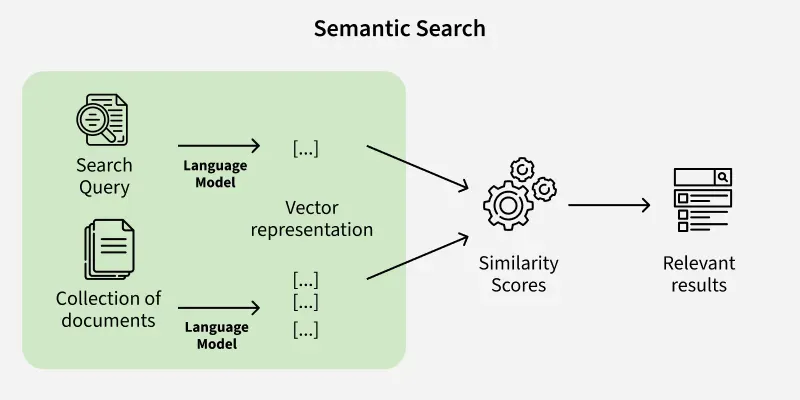
\includegraphics[width=0.75\textwidth]{Images/Kienthucnentang/Semantic-Search.png}
    \caption[Pipeline semantic search bao gồm các bước xử lý truy vấn, sinh embedding, truy xuất vector và xếp hạng kết quả dựa trên ngữ nghĩa]{Pipeline semantic search bao gồm các bước xử lý truy vấn, sinh embedding, truy xuất vector và xếp hạng kết quả dựa trên ngữ nghĩa \parencite{geeksforgeeks_semantic_search}}
    \label{fig:semantic_search_pipeline}
\end{figure}

Như minh họa trong \Cref{fig:semantic_search_pipeline}, semantic search sử dụng embedding vector để biểu diễn ngữ nghĩa của truy vấn và tài liệu trong không gian nhiều chiều, từ đó thực hiện semantic retrieval hiệu quả hơn keyword matching truyền thống.

Semantic search hiện là nền tảng quan trọng trong các hệ thống tìm kiếm thông minh, recommendation system và AI assistant hiện đại.
\subsubsection{Multimodal Search}

Multimodal Search là phương pháp tìm kiếm sử dụng nhiều loại dữ liệu như văn bản, hình ảnh và metadata để thực hiện truy hồi thông tin. Trong E-commerce, người dùng có thể tìm kiếm sản phẩm bằng hình ảnh hoặc kết hợp hình ảnh với mô tả văn bản như ``tìm áo giống hình này nhưng màu đen''.

Để giải quyết bài toán này, các hệ thống AI hiện đại thường sử dụng multimodal embedding nhằm ánh xạ dữ liệu từ nhiều modality vào cùng một semantic space. Các mô hình như CLIP sử dụng encoder riêng cho text và image, giúp các dữ liệu có ý nghĩa tương đồng được biểu diễn gần nhau trong vector space \cite{clip_paper}.

\begin{figure}[H]
    \centering
    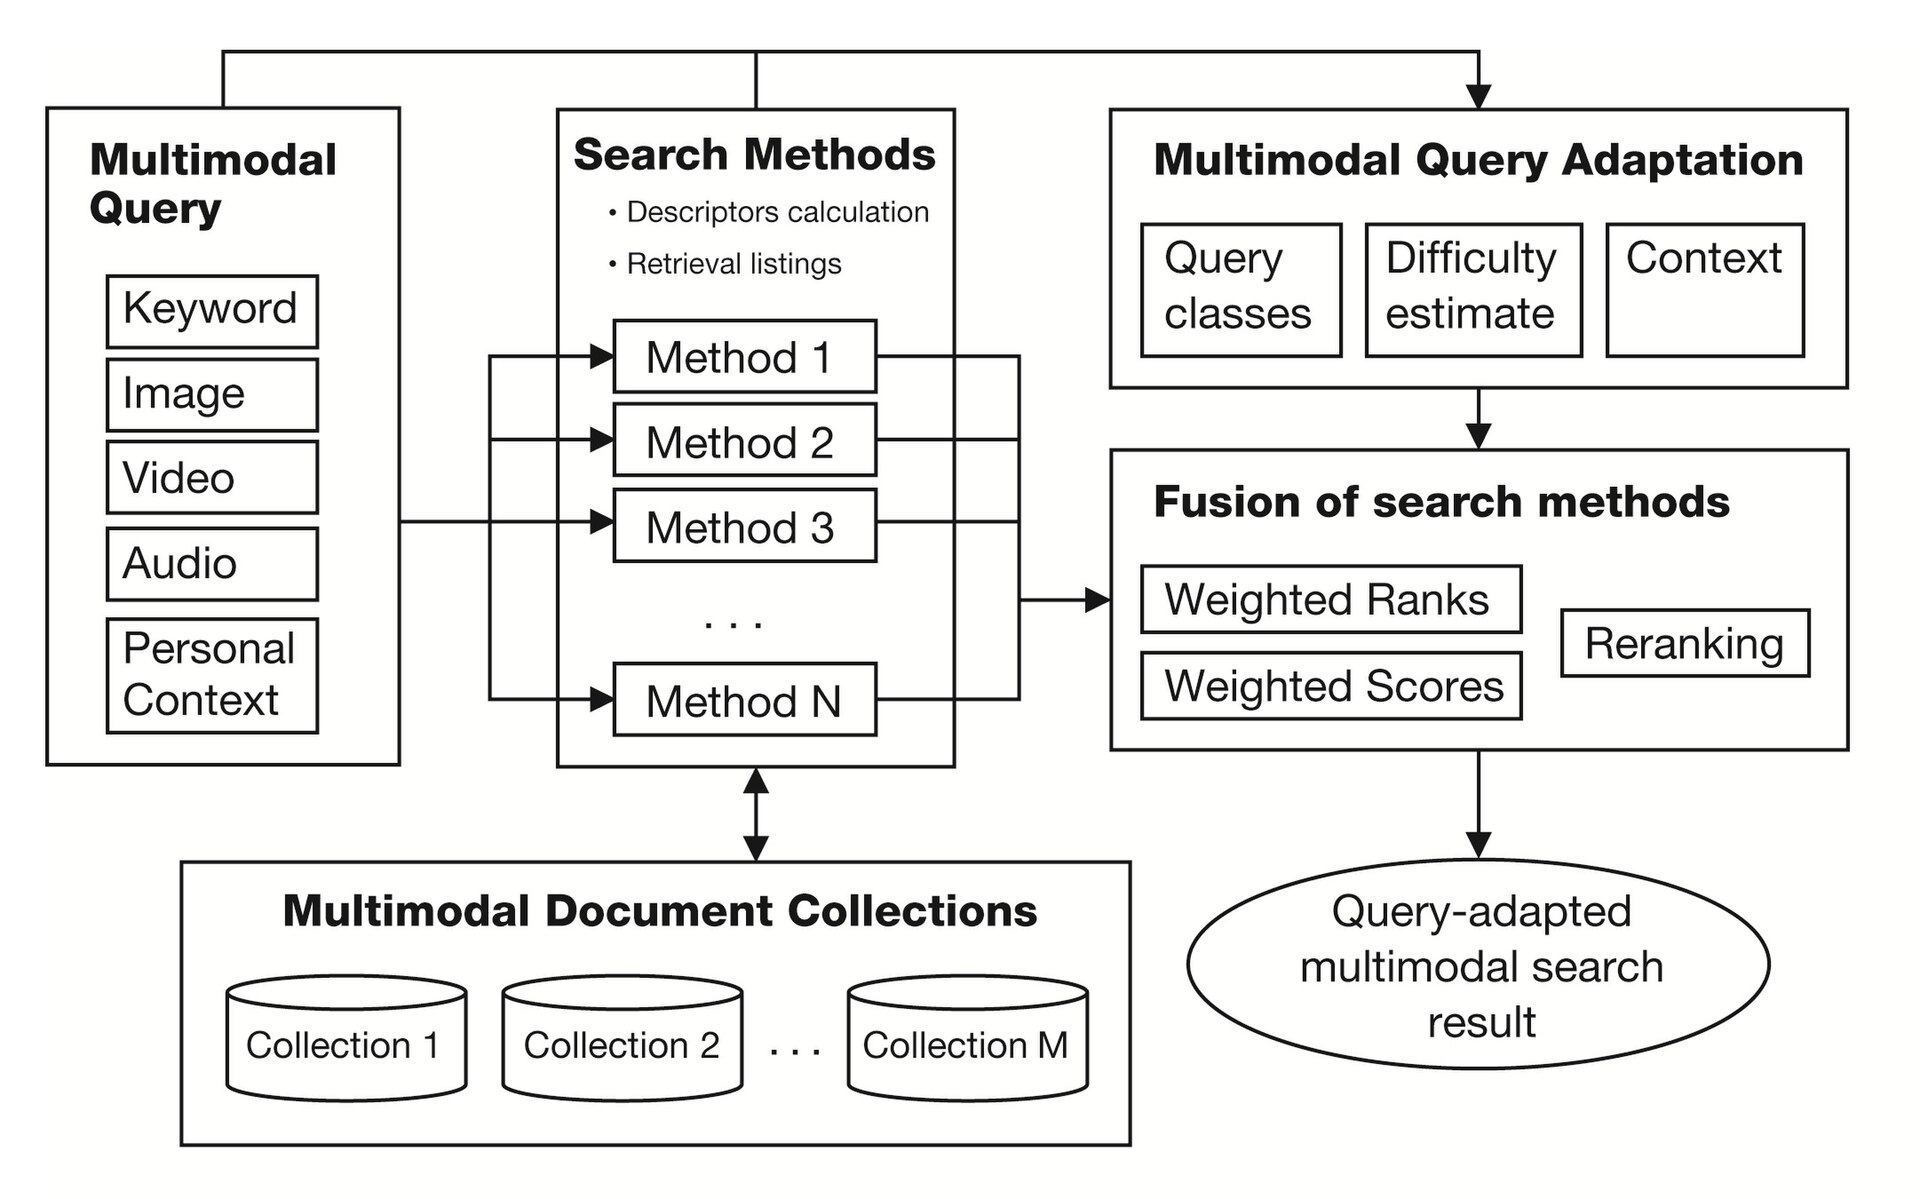
\includegraphics[width=0.7\textwidth]{Images/Kienthucnentang/Framework_of_Multimodal_Search.jpg}
    \caption[Framework của hệ thống multimodal search kết hợp truy vấn văn bản và hình ảnh nhằm cải thiện semantic retrieval trong E-commerce]{Framework của hệ thống multimodal search kết hợp truy vấn văn bản và hình ảnh nhằm cải thiện semantic retrieval trong E-commerce \parencite{ipullrank_mum_search}}
    \label{fig:framework_multimodal_search}
\end{figure}

Như trình bày trong \Cref{fig:framework_multimodal_search}, multimodal search kết hợp truy vấn văn bản và hình ảnh để cải thiện semantic retrieval thông qua embedding đa phương thức và vector retrieval.

Multimodal search hỗ trợ nhiều dạng truy hồi như text-to-image retrieval, image-to-image retrieval và hybrid retrieval, giúp cải thiện trải nghiệm tìm kiếm trong các hệ thống E-commerce hiện đại.
\subsubsection{Ứng dụng AI trong hệ thống tìm kiếm sản phẩm}

Trí tuệ nhân tạo đóng vai trò quan trọng trong các hệ thống tìm kiếm sản phẩm hiện đại. Khác với keyword-based search truyền thống, các hệ thống search dùng AI sử dụng embedding model và deep learning để khai thác ngữ nghĩa của truy vấn và dữ liệu sản phẩm.
Các ứng dụng AI phổ biến trong hệ thống E-commerce gồm:

\begin{itemize}
    \item \textbf{Semantic Search}: Hỗ trợ tìm kiếm sản phẩm dựa trên ý nghĩa của truy vấn thay vì chỉ đối sánh từ khóa.
    
    \item \textbf{Recommendation System}: Gợi ý sản phẩm phù hợp dựa trên hành vi người dùng, lịch sử tìm kiếm, lịch sử mua hàng hoặc sản phẩm tương tự.
    
    \item \textbf{Personalized Search}: Cá nhân hóa kết quả tìm kiếm theo sở thích, nhu cầu, vị trí, ngân sách hoặc lịch sử tương tác của từng người dùng.
    
    \item \textbf{Visual Search}: Cho phép người dùng tìm kiếm sản phẩm bằng hình ảnh, ví dụ tải lên ảnh một đôi giày hoặc chiếc túi để tìm sản phẩm tương tự.
    
    \item \textbf{Conversational AI Assistant}: Hỗ trợ người dùng tìm kiếm, so sánh và lựa chọn sản phẩm thông qua hội thoại tự nhiên.
\end{itemize}

AI giúp hệ thống hiểu ý định người dùng, phân tích ngữ cảnh truy vấn và cá nhân hóa kết quả tìm kiếm. Bên cạnh đó, sự phát triển của LLM và Conversational AI cho phép hỗ trợ hội thoại tự nhiên và tìm kiếm đa lượt hiệu quả hơn.

Việc kết hợp semantic search, recommendation system và multimodal retrieval hiện là xu hướng quan trọng trong các nền tảng E-commerce hiện đại.
\subsection{Hệ thống truy hồi thông tin}

% Hệ thống truy hồi thông tin (Information Retrieval -- IR) là lĩnh vực nghiên cứu tập trung vào việc tìm kiếm và truy xuất dữ liệu liên quan từ một tập dữ liệu lớn dựa trên truy vấn của người dùng \cite{manning_ir_book}. Trong lĩnh vực thương mại điện tử, hệ thống IR đóng vai trò quan trọng trong việc kết nối nhu cầu tìm kiếm của người dùng với cơ sở dữ liệu sản phẩm. Chất lượng của hệ thống truy hồi ảnh hưởng trực tiếp đến trải nghiệm người dùng, khả năng khám phá sản phẩm và hiệu quả recommendation.

% Khác với hệ quản trị cơ sở dữ liệu truyền thống chỉ truy xuất dữ liệu theo điều kiện chính xác, hệ thống IR tập trung vào việc đánh giá mức độ liên quan (relevance) giữa truy vấn và tài liệu. Điều này đặc biệt quan trọng trong các hệ thống tìm kiếm hiện đại khi người dùng thường sử dụng ngôn ngữ tự nhiên, truy vấn dài hoặc mô tả mang tính ngữ nghĩa thay vì các từ khóa cố định.

% Trong các hệ thống tìm kiếm hiện đại, Information Retrieval không chỉ bao gồm keyword matching truyền thống mà còn mở rộng sang semantic retrieval, vector retrieval, hybrid retrieval và reranking. Các hệ thống IR thường bao gồm các thành phần xử lý chính như:

% \begin{itemize}
%     \item Query processing
%     \item Candidate retrieval
%     \item Document ranking
%     \item Relevance refinement
%     \item Result presentation
% \end{itemize}

% Các phương pháp truy hồi truyền thống như TF-IDF hoặc BM25 chủ yếu dựa trên tần suất xuất hiện của từ khóa trong tài liệu \cite{bm25_paper}. Tuy nhiên, cùng với sự phát triển của deep learning và embedding model, nhiều hệ thống IR hiện đại đã chuyển sang sử dụng semantic embedding nhằm cải thiện khả năng hiểu ngữ nghĩa của truy vấn và dữ liệu.

% Ngoài độ chính xác retrieval, các hệ thống IR hiện đại còn phải đáp ứng nhiều yêu cầu khác như độ trễ thấp (low latency), khả năng mở rộng (scalability) và khả năng xử lý dữ liệu lớn trong thời gian thực. Đây là những yếu tố quan trọng trong các nền tảng thương mại điện tử và hệ thống tìm kiếm thông minh hiện nay.
% \subsubsection{Keyword-based Retrieval}

% Keyword-based Retrieval là phương pháp truy hồi thông tin truyền thống dựa trên việc đối sánh trực tiếp từ khóa truy vấn với nội dung dữ liệu \cite{manning_ir_book}. Đây là nền tảng của nhiều search engine cổ điển và vẫn được sử dụng rộng rãi trong các hệ thống tìm kiếm hiện nay nhờ tốc độ xử lý nhanh và chi phí tính toán thấp.

% Trong phương pháp này, hệ thống sẽ phân tích truy vấn của người dùng thành các token, sau đó tìm kiếm các tài liệu hoặc sản phẩm chứa các token tương ứng trong cơ sở dữ liệu. Để tăng tốc độ truy xuất, các hệ thống IR thường sử dụng cấu trúc dữ liệu inverted index \cite{lucene_docs}. Inverted index lưu ánh xạ giữa token và danh sách tài liệu chứa token đó, giúp giảm đáng kể thời gian tìm kiếm.

% Ví dụ, với truy vấn ``giày chạy bộ'', hệ thống sẽ tìm kiếm các tài liệu hoặc sản phẩm chứa các token như ``giày'', ``chạy'' và ``bộ'', sau đó tính toán mức độ liên quan dựa trên tần suất xuất hiện của từ khóa và các phương pháp xếp hạng như TF-IDF hoặc BM25 \cite{bm25_paper}.

% Ưu điểm của keyword-based retrieval bao gồm:

% \begin{itemize}
%     \item Tốc độ truy xuất nhanh
%     \item Dễ triển khai và tối ưu hóa
%     \item Chi phí tính toán thấp
%     \item Hoạt động hiệu quả với exact keyword matching
% \end{itemize}

% Tuy nhiên, keyword-based retrieval tồn tại nhiều hạn chế trong các hệ thống tìm kiếm hiện đại. Phương pháp này chủ yếu dựa trên token matching và không hiểu được ngữ nghĩa thực sự của truy vấn. Điều này làm giảm hiệu quả retrieval trong các trường hợp như:

% \begin{itemize}
%     \item Synonym và từ đồng nghĩa
%     \item Natural language query
%     \item Contextual meaning
%     \item Multilingual query
%     \item Conversational search
% \end{itemize}

% Ví dụ, các truy vấn như ``running shoes'', ``sports sneakers'' và ``giày chạy bộ'' có thể mang cùng ý nghĩa ngữ nghĩa nhưng lại được xem là các tập từ khóa khác nhau trong keyword retrieval truyền thống.

% Do những hạn chế về khả năng hiểu ngữ nghĩa, nhiều hệ thống tìm kiếm hiện đại thường kết hợp keyword-based retrieval với semantic retrieval nhằm tận dụng ưu điểm của cả hai phương pháp. Hướng tiếp cận này thường được gọi là hybrid search, trong đó keyword retrieval hỗ trợ xử lý exact matching còn semantic retrieval cải thiện khả năng hiểu ngữ cảnh và ý định truy vấn.
\subsubsection{BM25}

BM25 là một thuật toán xếp hạng được sử dụng phổ biến trong các hệ thống Information Retrieval truyền thống. Thuật toán này đánh giá mức độ liên quan giữa truy vấn và tài liệu dựa trên sự xuất hiện của từ khóa, đồng thời xét đến độ dài tài liệu để tránh việc các tài liệu dài luôn được ưu tiên hơn.

So với TF-IDF truyền thống, BM25 cải thiện khả năng xếp hạng nhờ cơ chế chuẩn hóa độ dài tài liệu, giảm ảnh hưởng của các từ xuất hiện quá nhiều và tối ưu điểm liên quan giữa truy vấn với tài liệu. Điểm BM25 thường được tính dựa trên ba yếu tố chính là tần suất xuất hiện của từ khóa trong tài liệu, mức độ hiếm của từ khóa trong toàn bộ tập tài liệu và độ dài của tài liệu.

Công thức tính điểm BM25 thường được biểu diễn như sau \cite{robertson2009probabilistic}:

\begin{equation}
\text{BM25}(q,d)=\sum_{t \in q} IDF(t)\cdot
\frac{f(t,d)\cdot (k_1+1)}
{f(t,d)+k_1\cdot
\left(1-b+b\cdot \frac{|d|}{avgdl}\right)}
\label{eq:bm25}
\end{equation}

Trong đó, $f(t,d)$ là số lần từ khóa $t$ xuất hiện trong tài liệu $d$, $|d|$ là độ dài tài liệu, $avgdl$ là độ dài tài liệu trung bình trong toàn bộ tập dữ liệu. Hai tham số $k_1$ và $b$ được dùng để điều chỉnh ảnh hưởng của tần suất từ khóa và mức độ chuẩn hóa theo độ dài tài liệu.

BM25 phù hợp với các truy vấn chứa từ khóa rõ ràng như tên sản phẩm, thương hiệu, mã sản phẩm hoặc thông số kỹ thuật. Tuy nhiên, do chủ yếu dựa trên token matching, BM25 còn hạn chế khi xử lý truy vấn ngôn ngữ tự nhiên, từ đồng nghĩa hoặc truy vấn phụ thuộc ngữ cảnh. Vì vậy, trong các hệ thống tìm kiếm hiện đại, BM25 thường được kết hợp với semantic retrieval để tạo thành hybrid retrieval.
\subsubsection{Semantic Retrieval}

Semantic Retrieval là phương pháp truy hồi thông tin dựa trên ngữ nghĩa thay vì chỉ đối sánh từ khóa trực tiếp như keyword-based retrieval truyền thống. Trong phương pháp này, truy vấn và tài liệu được biểu diễn dưới dạng vector embedding trong semantic space, nơi các dữ liệu có ý nghĩa tương đồng sẽ nằm gần nhau.

Semantic retrieval thường bao gồm các bước như query embedding, document embedding, vector similarity search và relevance ranking.
\begin{figure}[H]
    \centering
    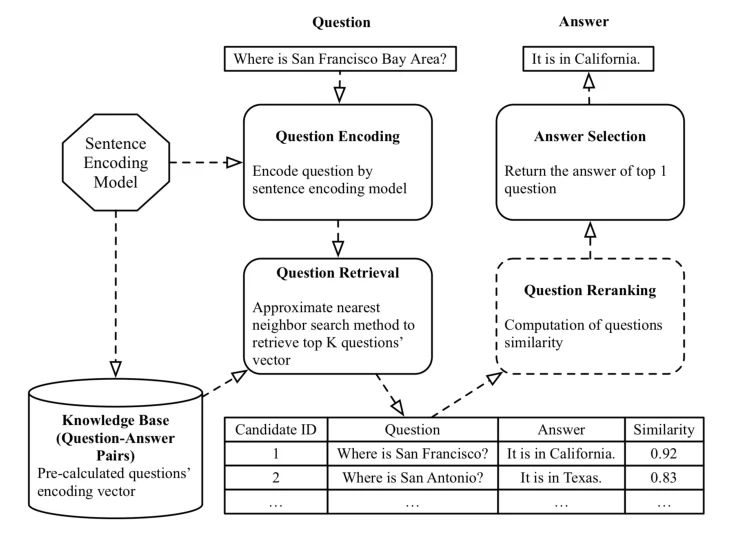
\includegraphics[width=0.65\textwidth]{Images/Kienthucnentang/semantic-retrieval.png}
    \caption[Workflow của semantic retrieval QA system bao gồm các bước embedding, semantic matching và retrieval]{Workflow của semantic retrieval QA system bao gồm các bước embedding, semantic matching và retrieval \parencite{semantic_retrieval_rg}}
    \label{fig:semantic_retrieval_workflow}
\end{figure}

Như minh họa trong \Cref{fig:semantic_retrieval_workflow}, semantic retrieval thực hiện truy xuất dựa trên độ tương đồng giữa các vector embedding thay vì chỉ dựa trên token matching truyền thống.
Ví dụ, với truy vấn ``áo khoác mùa đông'', hệ thống vẫn có thể truy hồi các sản phẩm như hoodie hoặc jacket dù không chứa chính xác từ khóa truy vấn.

Semantic retrieval giúp cải thiện khả năng hiểu ngữ nghĩa, hỗ trợ natural language query và tăng chất lượng retrieval trong các hệ thống tìm kiếm hiện đại. Tuy nhiên, việc xử lý vector embedding cũng làm tăng chi phí tính toán, do đó nhiều hệ thống hiện nay thường kết hợp semantic retrieval với keyword-based retrieval theo hướng hybrid retrieval.
% \subsubsection{Hybrid Search}

% Hybrid Search là phương pháp truy hồi thông tin kết hợp giữa keyword-based retrieval và semantic retrieval nhằm tận dụng ưu điểm của cả hai phương pháp \cite{hybrid_search_pinecone}.

% Trong khi keyword retrieval phù hợp với exact keyword hoặc brand name, semantic retrieval có khả năng xử lý ngữ nghĩa và natural language query tốt hơn. Hybrid search kết hợp sparse retrieval và dense retrieval để cải thiện chất lượng retrieval tổng thể.

% Hệ thống hybrid retrieval thường bao gồm BM25 retrieval, dense vector retrieval và fusion strategy như RRF.

% Ví dụ, với truy vấn ``nike running shoes under 2 million'', keyword retrieval hỗ trợ đối sánh thương hiệu ``Nike'', trong khi semantic retrieval giúp hiểu ngữ nghĩa của cụm ``running shoes''. Nhờ đó, hybrid search giúp cải thiện độ chính xác và hiệu quả retrieval trong các hệ thống tìm kiếm hiện đại.
% \subsubsection{Reranking}

% Reranking là giai đoạn sắp xếp lại các candidate document trong retrieval pipeline nhằm cải thiện mức độ liên quan giữa truy vấn và kết quả truy hồi \cite{reranking_sbert}.

% Thông thường, hệ thống retrieval gồm hai giai đoạn: first-stage retrieval để truy hồi top-k candidate nhanh chóng và second-stage reranking để đánh giá lại mức độ liên quan của từng kết quả.

% Khác với retrieval model chỉ dựa trên vector similarity, reranking thường sử dụng cross-encoder architecture để phân tích trực tiếp mối quan hệ giữa query và document, từ đó tính toán relevance score chính xác hơn.

% Ví dụ, với truy vấn ``giày chạy bộ cho người mới'', reranking model có thể ưu tiên các sản phẩm phù hợp với người mới thay vì các mẫu dành cho vận động viên chuyên nghiệp.

% Reranking giúp cải thiện retrieval precision và giảm irrelevant retrieval trong các hệ thống semantic search hiện đại. Tuy nhiên, do chi phí tính toán cao, phương pháp này thường chỉ áp dụng trên tập top-k candidate retrieval.
% \subsubsection{Đánh giá hệ thống truy hồi thông tin}

% Đánh giá hệ thống Information Retrieval (IR) là bước quan trọng nhằm đo lường hiệu quả retrieval của hệ thống tìm kiếm \cite{manning_ir_book}. Trong các hệ thống AI Search hiện đại, việc đánh giá không chỉ tập trung vào độ chính xác retrieval mà còn xem xét hiệu năng xử lý và khả năng đáp ứng yêu cầu thời gian thực.

% Các hệ thống IR thường được đánh giá dựa trên nhiều nhóm metric khác nhau, bao gồm retrieval effectiveness và system performance.

% \textbf{Precision}

% Precision đo tỷ lệ kết quả liên quan trong tập kết quả retrieval. Metric này phản ánh mức độ chính xác của hệ thống khi trả về các tài liệu hoặc sản phẩm phù hợp với truy vấn người dùng.

% Ví dụ, nếu hệ thống trả về top-10 kết quả và có 8 kết quả liên quan, precision sẽ bằng 0.8.

% \textbf{Recall}

% Recall đo khả năng truy hồi đầy đủ các tài liệu liên quan trong toàn bộ corpus.

% Metric này đặc biệt quan trọng trong các hệ thống semantic retrieval vì mục tiêu không chỉ là trả về kết quả chính xác mà còn hạn chế bỏ sót các tài liệu liên quan.

% \textbf{MRR (Mean Reciprocal Rank)}

% MRR được sử dụng để đánh giá vị trí xuất hiện của kết quả đúng đầu tiên trong danh sách retrieval.

% MRR có ý nghĩa quan trọng trong các hệ thống tìm kiếm sản phẩm hoặc question answering, nơi người dùng thường ưu tiên các kết quả đầu tiên.

% \textbf{nDCG (Normalized Discounted Cumulative Gain)}

% nDCG là metric đánh giá chất lượng ranking dựa trên mức độ liên quan và vị trí của kết quả retrieval.

% Metric này cho phép đánh giá chất lượng xếp hạng trong các hệ thống retrieval có nhiều mức relevance khác nhau.

% Ngoài các retrieval metric, hệ thống IR hiện đại còn được đánh giá dựa trên các yếu tố hiệu năng như:

% \begin{itemize}
%     \item Latency
%     \item Throughput
%     \item Scalability
%     \item Resource utilization
% \end{itemize}

% Trong các hệ thống AI Shopping Assistant, retrieval quality ảnh hưởng trực tiếp đến chất lượng tìm kiếm, recommendation và phản hồi của hệ thống RAG. Vì vậy, việc lựa chọn metric đánh giá phù hợp đóng vai trò quan trọng trong quá trình tối ưu hệ thống retrieval.

% Nhiều benchmark Information Retrieval hiện đại như BEIR được sử dụng để đánh giá retrieval model trên nhiều domain và retrieval task khác nhau \cite{beir_benchmark}.
\subsection{Vector Embedding và Semantic Representation}
\subsubsection{Khái niệm Vector Embedding}

Trong các hệ thống AI Search hiện đại, dữ liệu thường được chuyển đổi thành các vector số học nhằm hỗ trợ máy tính biểu diễn và xử lý ngữ nghĩa của dữ liệu \cite{bert_paper}. Vector embedding là phương pháp ánh xạ dữ liệu như văn bản hoặc hình ảnh thành các vector trong không gian nhiều chiều, trong đó khoảng cách giữa các vector phản ánh mức độ tương đồng ngữ nghĩa giữa các đối tượng dữ liệu.

Khác với các phương pháp biểu diễn truyền thống, embedding cho phép mô hình học được mối quan hệ ngữ nghĩa giữa dữ liệu. Nhờ đó, các cụm từ như ``giày chạy bộ'', ``running shoes'' hay ``sports sneakers'' có thể được biểu diễn bằng các vector gần nhau dù sử dụng từ khác nhau.

Embedding đóng vai trò quan trọng trong semantic retrieval và multimodal search. Sau khi dữ liệu được embedding hóa, hệ thống có thể thực hiện similarity search hoặc vector retrieval để tìm các đối tượng có mức độ tương đồng cao trong semantic space.

Hiện nay, vector embedding được ứng dụng rộng rãi trong semantic search, recommendation system, chatbot và RAG.
\subsubsection{Semantic Space}

Semantic space là không gian biểu diễn vector trong đó khoảng cách giữa các vector phản ánh mức độ tương đồng ngữ nghĩa giữa các dữ liệu \cite{pinecone_embedding}. Sau khi dữ liệu được embedding hóa, các vector sẽ được ánh xạ vào semantic space để phục vụ các bài toán semantic retrieval và similarity search.

Ý tưởng cốt lõi của semantic space là các dữ liệu có nội dung tương tự sẽ nằm gần nhau trong không gian vector dù sử dụng cách biểu diễn khác nhau. Ví dụ, các cụm từ như ``laptop gaming'', ``gaming notebook'' và ``máy tính chơi game'' có thể được biểu diễn bằng các vector gần nhau do mang ý nghĩa tương đồng.

Để đo mức độ tương đồng giữa các vector trong semantic space, các hệ thống retrieval thường sử dụng các phép đo như:

\begin{itemize}
    \item Cosine Similarity
    \item Euclidean Distance
    \item Dot Product
\end{itemize}

Trong đó, Cosine Similarity là phương pháp phổ biến nhất trong semantic retrieval do tập trung đo sự tương đồng về hướng của vector thay vì độ lớn tuyệt đối.

Một đặc điểm quan trọng của semantic space là hiện tượng semantic clustering, trong đó các vector có cùng chủ đề hoặc đặc trưng dữ liệu thường hình thành các cụm trong không gian vector. Điều này hỗ trợ hiệu quả cho các hệ thống semantic search và recommendation system.

Tuy nhiên, khi số lượng vector tăng lên rất lớn, việc tìm kiếm nearest neighbors trong semantic space trở nên tốn kém về mặt tính toán. Vì vậy, các hệ thống hiện đại thường sử dụng vector database và ANN indexing nhằm tối ưu tốc độ retrieval.
\subsubsection{Text Embedding}

Text Embedding là kỹ thuật chuyển đổi văn bản thành vector số thực nhằm biểu diễn ngữ nghĩa của câu, đoạn văn hoặc tài liệu trong không gian vector. Đây là nền tảng quan trọng của nhiều hệ thống NLP hiện đại như semantic search, recommendation system, chatbot và RAG.

Khác với các phương pháp truyền thống như bag-of-words hoặc TF-IDF, text embedding cho phép mô hình học được semantic representation của ngôn ngữ tự nhiên. Nhờ đó, các câu hoặc cụm từ có ý nghĩa tương đồng sẽ được biểu diễn gần nhau trong semantic space.

Trong hệ thống AI Shopping Assistant, text embedding được sử dụng để biểu diễn product title, product description, user query và conversational context.

Ví dụ, các truy vấn như ``running shoes'', ``sports sneakers'' và ``giày chạy bộ'' có thể được ánh xạ gần nhau trong semantic space.

Hiện nay, nhiều hệ thống semantic search sử dụng transformer-based embedding model như BERT hoặc Sentence-BERT nhằm cải thiện chất lượng semantic retrieval.
\subsubsection{Image Embedding}

Image Embedding là kỹ thuật chuyển đổi hình ảnh thành vector số thực nhằm biểu diễn đặc trưng trực quan và ngữ nghĩa của ảnh trong không gian vector. Đây là nền tảng quan trọng trong các hệ thống computer vision hiện đại như image retrieval, visual search và multimodal AI.

Khác với các phương pháp xử lý ảnh truyền thống, image embedding sử dụng deep learning để tự động học đặc trưng của hình ảnh. Các hình ảnh có nội dung tương tự sẽ được biểu diễn bằng các vector nằm gần nhau trong semantic space.

Trong hệ thống AI Shopping Assistant, image embedding được sử dụng để biểu diễn product image, user uploaded image và visual feature representation.

Ví dụ, khi người dùng tải lên hình ảnh của một đôi giày thể thao, hệ thống sẽ chuyển đổi hình ảnh thành vector embedding và thực hiện similarity search để tìm các sản phẩm tương tự.

Hiện nay, nhiều hệ thống AI hiện đại sử dụng các mô hình như CLIP, ViT hoặc CNN để xây dựng image embedding phục vụ visual search và multimodal retrieval.
\subsubsection{Multimodal Embedding}

Multimodal Embedding là kỹ thuật biểu diễn nhiều loại dữ liệu như văn bản và hình ảnh trong cùng một semantic space. Đây là nền tảng quan trọng của các hệ thống multimodal AI và cross-modal retrieval hiện đại.

Trong multimodal embedding, hệ thống sử dụng các encoder riêng cho text và image nhưng được huấn luyện để tạo ra embedding trong cùng không gian vector. Nhờ đó, dữ liệu có cùng ý nghĩa ngữ nghĩa sẽ được biểu diễn gần nhau dù thuộc các modality khác nhau.

Ví dụ, truy vấn ``áo hoodie màu đen'' và hình ảnh của một áo hoodie đen có thể được ánh xạ thành các vector gần nhau trong semantic space.

Multimodal embedding hỗ trợ nhiều bài toán như text-to-image retrieval, image-to-text retrieval và hybrid search. Trong E-commerce, kỹ thuật này giúp người dùng tìm kiếm sản phẩm linh hoạt hơn bằng cách kết hợp văn bản và hình ảnh.

Hiện nay, nhiều mô hình như CLIP, SigLIP hoặc ALIGN được sử dụng để xây dựng multimodal embedding phục vụ semantic retrieval và multimodal search.
% \subsubsection{Tiêu chí lựa chọn mô hình Text Embedding}
% Việc lựa chọn mô hình text embedding là bước quan trọng trong quá trình xây dựng hệ thống AI Search và semantic retrieval. Một mô hình embedding phù hợp không chỉ ảnh hưởng đến độ chính xác retrieval mà còn tác động trực tiếp đến latency, scalability và chi phí triển khai của hệ thống.

% Tiêu chí đầu tiên cần xem xét là semantic performance. Đây là yếu tố quan trọng nhất trong các hệ thống AI Search hiện đại vì mục tiêu chính của embedding là biểu diễn ngữ nghĩa của dữ liệu. Mô hình cần có khả năng đưa các câu hoặc truy vấn có ý nghĩa tương tự đến gần nhau trong semantic space. Trong bài toán thương mại điện tử, điều này đặc biệt quan trọng vì người dùng thường sử dụng truy vấn ngôn ngữ tự nhiên thay vì exact keyword.

% Tiêu chí thứ hai là retrieval quality. Một mô hình embedding tốt cần tối ưu cho semantic retrieval thay vì chỉ phục vụ NLP thông thường. Các mô hình được huấn luyện bằng contrastive learning như BGE hoặc E5 thường cho hiệu quả retrieval cao hơn trong các bài toán vector search và RAG.

% Embedding dimension cũng là yếu tố quan trọng cần cân nhắc. Vector dimension càng lớn thì khả năng biểu diễn semantic càng mạnh nhưng đồng thời cũng làm tăng:
% Các tiêu chí quan trọng:
% \begin{itemize}
%     \item Bộ nhớ lưu trữ vector
%     \item Chi phí ANN indexing
%     \item Latency retrieval
%     \item GPU memory usage
% \end{itemize}

% Ví dụ, embedding 3072 chiều sẽ yêu cầu nhiều tài nguyên hơn embedding 384 chiều khi lưu trữ hàng triệu sản phẩm trong vector database. Vì vậy, hệ thống thực tế thường cần cân bằng giữa semantic quality và scalability

% Latency và inference speed cũng là tiêu chí quan trọng trong hệ thống E-commerce Search thời gian thực. Người dùng thường kỳ vọng kết quả tìm kiếm được trả về trong vài trăm milliseconds. Do đó, embedding model cần đủ nhẹ để inference nhanh nhưng vẫn đảm bảo semantic quality. Các mô hình small hoặc base thường phù hợp hơn large model trong môi trường production do tối ưu tốt hơn về tốc độ và chi phí vận hành.

% Khả năng hỗ trợ multilingual retrieval là tiêu chí cần thiết trong các hệ thống thương mại điện tử đa ngôn ngữ. Người dùng có thể tìm kiếm bằng tiếng Anh, tiếng Việt hoặc kết hợp nhiều ngôn ngữ khác nhau. Các mô hình như multilingual-E5 hoặc BGE-M3 thường có ưu thế trong các bài toán multilingual semantic search.

% Ngoài ra, khả năng self-hosting và triển khai nội bộ cũng là yếu tố quan trọng trong nhiều hệ thống doanh nghiệp. Open-source embedding model như BGE hoặc E5 cho phép triển khai trực tiếp trên server nội bộ, giúp:

% \begin{itemize}
%     \item Giảm chi phí API
%     \item Bảo vệ dữ liệu người dùng
%     \item Tùy chỉnh theo domain riêng
%     \item Chủ động tối ưu pipeline retrieval
% \end{itemize}

% Trong đồ án AI Shopping Assistant, mô hình BGE được lựa chọn do đáp ứng tốt các tiêu chí:
% \begin{itemize}
%     \item Semantic retrieval mạnh
%     \item Tối ưu cho dense retrieval
%     \item Hỗ trợ multilingual
%     \item Hoạt động tốt với vector database
%     \item Phù hợp hybrid search và RAG pipeline
%     \item Có phiên bản lightweight cho inference nhanh
% \end{itemize}
% Ngoài ra, BGE có hệ sinh thái hỗ trợ tốt cho semantic search và retrieval engineering, giúp dễ dàng tích hợp với Qdrant, LangChain và các vector database hiện đại
% \subsubsection{Tiêu chí lựa chọn mô hình Image Embedding}

% Khi lựa chọn mô hình embedding cho hệ thống AI search hoặc CBIR, cần cân nhắc các yếu tố sau:

% \begin{itemize}
%     \item \textbf{Độ chính xác (Accuracy)}
%     \item \textbf{Tốc độ suy luận (Inference speed)}
%     \item \textbf{Khả năng mở rộng (Scalability)}
%     \item \textbf{Chi phí huấn luyện}
%     \item \textbf{Tính sẵn có của pretrained model}
% \end{itemize}

% Trong thực tế, các hệ thống thương mại thường sử dụng:
% \begin{itemize}
%     \item CNN (ResNet, EfficientNet) cho baseline
%     \item Vision Transformer hoặc CLIP cho semantic search nâng cao
% \end{itemize}
\subsection{Multimodal Search trong E-commerce}

\subsubsection{Text-Image Retrieval}

Text-Image Retrieval là bài toán truy xuất dữ liệu giữa văn bản và hình ảnh, trong đó hệ thống thực hiện tìm kiếm hình ảnh từ văn bản hoặc tìm kiếm văn bản từ hình ảnh \parencite{faghri2018vsepp}.

Mục tiêu của phương pháp này là học mối quan hệ ngữ nghĩa giữa text và image bằng cách ánh xạ chúng vào cùng một semantic embedding space. Trong không gian này, các cặp dữ liệu có liên quan sẽ có khoảng cách vector gần nhau hơn.

Trong hệ thống retrieval hiện đại, văn bản thường được xử lý bởi text encoder và hình ảnh được xử lý bởi image encoder nhằm trích xuất semantic feature cho từng modality.

Các thành phần chính của text-image retrieval gồm:
\begin{itemize}
    \item Text Representation
    \item Image Representation
    \item Shared Embedding Space
    \item Similarity Measurement
\end{itemize}

\begin{figure}[H]
    \centering
    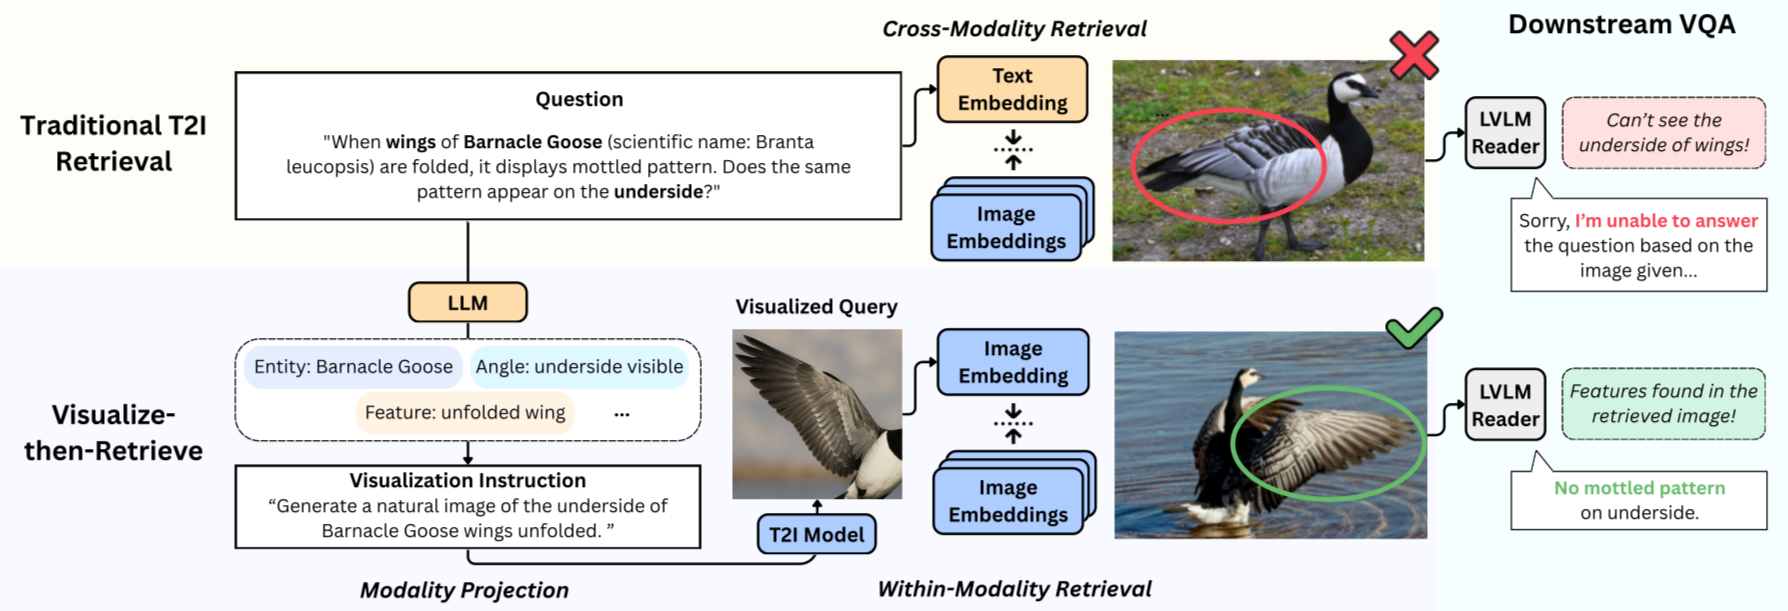
\includegraphics[width=0.75\linewidth]{Images/Kienthucnentang/text-image-retrieval.png}
    \caption[Bài toán Text-Image Retrieval với quá trình ánh xạ văn bản và hình ảnh vào cùng không gian ngữ nghĩa để thực hiện truy xuất liên modality]{Bài toán Text-Image Retrieval với quá trình ánh xạ văn bản và hình ảnh vào cùng không gian ngữ nghĩa để thực hiện truy xuất liên modality \cite{moonlight2024visualizedretrieval}}
    \label{fig:text-image-retrieval}
\end{figure}

Như minh họa ở \Cref{fig:text-image-retrieval}, text-image retrieval hỗ trợ liên kết dữ liệu văn bản và hình ảnh nhằm phục vụ các hệ thống multimodal search và E-commerce retrieval hiện đại.
\subsubsection{Computer Vision và Object Detection trong E-commerce}

Computer Vision là lĩnh vực cho phép máy tính phân tích và hiểu thông tin từ hình ảnh hoặc video. Trong thương mại điện tử, Computer Vision được ứng dụng nhằm hỗ trợ phân tích sản phẩm, visual search, visual recommendation và hiểu nội dung hình ảnh sản phẩm.

Dữ liệu hình ảnh đóng vai trò quan trọng trong E-commerce vì người dùng thường đưa ra quyết định mua sắm dựa trên thông tin trực quan. Các kỹ thuật Computer Vision giúp hệ thống khai thác các đặc trưng thị giác như màu sắc, hình dạng, kết cấu, kiểu dáng hoặc phong cách của sản phẩm từ dữ liệu hình ảnh. Những đặc trưng này có thể được sử dụng để tìm kiếm sản phẩm tương tự, phân loại sản phẩm hoặc hỗ trợ hệ thống gợi ý sản phẩm theo ngữ cảnh thị giác.

Trong các hệ thống E-commerce hiện đại, Computer Vision thường được sử dụng cho các bài toán:
\begin{itemize}
    \item Nhận dạng và phân loại sản phẩm
    \item Tìm kiếm sản phẩm bằng hình ảnh
    \item Phân tích thuộc tính thị giác của sản phẩm
    \item Phát hiện đối tượng trong ảnh sản phẩm
    \item Visual recommendation và visual retrieval
\end{itemize}
\begin{figure}[H]
    \centering
    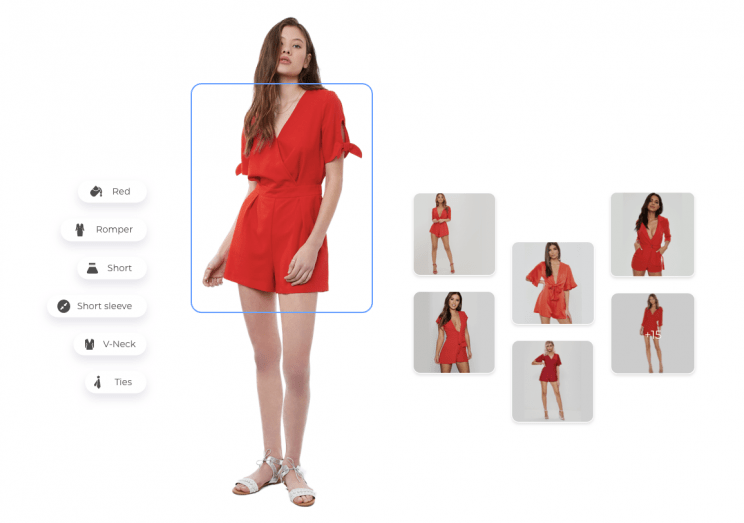
\includegraphics[width=0.7\textwidth]{Images/Kienthucnentang/visual-search-ecommerce.png}
    \caption[Ứng dụng Computer Vision trong tìm kiếm sản phẩm bằng hình ảnh trong E-commerce]{Ứng dụng Computer Vision trong tìm kiếm sản phẩm bằng hình ảnh trong E-commerce \parencite{cleed2024visualsearch}}
    \label{fig:visual-search-ecommerce}
\end{figure}
Một thành phần quan trọng của Computer Vision là visual feature representation, trong đó hình ảnh được chuyển đổi thành vector đặc trưng để biểu diễn nội dung thị giác trong không gian nhiều chiều. Các vector này hỗ trợ việc đo độ tương đồng giữa các hình ảnh và phục vụ semantic retrieval trong hệ thống AI Shopping Assistant.

Trong phạm vi Computer Vision, Object Detection là bài toán nhằm xác định vị trí và phân loại các đối tượng xuất hiện trong hình ảnh hoặc video \parencite{redmon2016yolo}. Khác với image classification chỉ dự đoán nhãn cho toàn bộ ảnh, Object Detection yêu cầu hệ thống vừa nhận diện loại đối tượng vừa xác định vị trí của chúng thông qua bounding box.

Trong Object Detection, mô hình thường thực hiện hai nhiệm vụ chính:
\begin{itemize}
    \item \textbf{Localization}: Xác định vị trí đối tượng trong ảnh.
    \item \textbf{Classification}: Phân loại đối tượng được phát hiện.
\end{itemize}

Kết quả của Object Detection thường bao gồm nhãn đối tượng, tọa độ bounding box và confidence score. Các thành phần quan trọng của Object Detection gồm feature extraction, bounding box regression và object classification. Một số mô hình còn sử dụng region proposal hoặc dense prediction để xác định các vùng có khả năng chứa đối tượng.

Các mô hình Object Detection hiện đại thường được chia thành hai nhóm chính:
\begin{itemize}
    \item \textbf{Two-stage Detector}: thực hiện đề xuất vùng trước, sau đó phân loại và tinh chỉnh bounding box, ví dụ như R-CNN và Faster R-CNN.
    \item \textbf{One-stage Detector}: dự đoán trực tiếp bounding box và nhãn đối tượng trong một lần xử lý, ví dụ như YOLO và SSD.
\end{itemize}

Trong đó, YOLO là một trong những mô hình Object Detection phổ biến nhờ khả năng xử lý thời gian thực và hiệu quả cao trong nhiều bài toán Computer Vision. Đối với E-commerce, Object Detection có thể được sử dụng để phát hiện sản phẩm trong ảnh, nhận diện nhiều sản phẩm xuất hiện cùng lúc, trích xuất vùng ảnh chứa sản phẩm chính và hỗ trợ tìm kiếm sản phẩm bằng hình ảnh. Ví dụ, khi người dùng tải lên một bức ảnh có chứa áo, giày hoặc túi xách, hệ thống có thể phát hiện từng đối tượng trong ảnh, cắt vùng liên quan và sử dụng đặc trưng thị giác của đối tượng đó để truy xuất các sản phẩm tương tự trong cơ sở dữ liệu.

Như vậy, Computer Vision cung cấp nền tảng tổng quát để hệ thống hiểu dữ liệu hình ảnh, trong khi Object Detection đóng vai trò là một kỹ thuật cụ thể giúp nhận diện và định vị sản phẩm trong ảnh. Sự kết hợp này giúp cải thiện khả năng visual search, product retrieval và trải nghiệm mua sắm trực quan trong các hệ thống E-commerce hiện đại.
\subsection{Vector Database và ANN Search}

\subsubsection{Khái niệm Vector Database}

Vector Database là loại cơ sở dữ liệu dùng để quản lý các vector embedding được tạo ra từ dữ liệu như văn bản, hình ảnh hoặc sản phẩm \parencite{wang2021milvus}. Thay vì chỉ tìm kiếm theo điều kiện khớp chính xác như cơ sở dữ liệu truyền thống, Vector Database cho phép truy xuất các đối tượng có mức độ tương đồng cao trong không gian vector. Nhờ đó, hệ thống có thể tìm ra những kết quả gần nghĩa hoặc gần đặc trưng với truy vấn đầu vào.

Trong các hệ thống AI hiện đại, dữ liệu như văn bản hoặc hình ảnh thường được chuyển đổi thành embedding vector nhằm biểu diễn semantic feature của dữ liệu. Các vector này cho phép hệ thống thực hiện semantic search và retrieval hiệu quả hơn keyword matching truyền thống.

Vector database đóng vai trò quan trọng trong semantic search, recommendation system, multimodal retrieval và RAG. Thay vì tìm kiếm theo từ khóa chính xác, hệ thống sẽ truy xuất các vector có khoảng cách gần nhất với vector truy vấn trong embedding space.

Các thành phần chính của vector database gồm:
\begin{itemize}
    \item Vector Embedding
    \item Vector Index
    \item Similarity Search
    \item High-dimensional Space
\end{itemize}

Trong không gian vector, các dữ liệu có ý nghĩa tương đồng thường được biểu diễn gần nhau hơn, giúp hệ thống hỗ trợ semantic retrieval hiệu quả.
\subsubsection{Độ tương đồng vector và Vector Similarity}

Sau khi dữ liệu được biểu diễn dưới dạng vector embedding, hệ thống AI Search cần một phương pháp để so sánh mức độ gần nhau giữa các vector. Việc đo độ tương đồng này giúp hệ thống xác định những sản phẩm, tài liệu hoặc truy vấn có ý nghĩa gần nhau, từ đó hỗ trợ các tác vụ như semantic retrieval và recommendation system.

Trong hệ thống tìm kiếm sản phẩm, truy vấn của người dùng sẽ được embedding hóa thành vector và so sánh với các vector sản phẩm trong vector database. Các vector có khoảng cách gần nhau hơn sẽ được xem là có mức độ liên quan cao hơn.

Khác với keyword matching truyền thống, vector similarity cho phép hệ thống hiểu semantic meaning thay vì exact keyword. Ví dụ, các cụm từ như ``running shoes'', ``sports sneakers'' và ``giày chạy bộ'' có thể được đánh giá tương đồng dù sử dụng từ khác nhau.

Một số phép đo vector similarity phổ biến gồm:
\begin{itemize}
    \item \textbf{Cosine Similarity}
    \item \textbf{Euclidean Distance}
    \item \textbf{Dot Product}
\end{itemize}

Trong đó, Cosine Similarity là phương pháp được sử dụng phổ biến trong semantic retrieval do khả năng đánh giá mức độ tương đồng ngữ nghĩa giữa các vector embedding.

\begin{figure}[H]
    \centering
    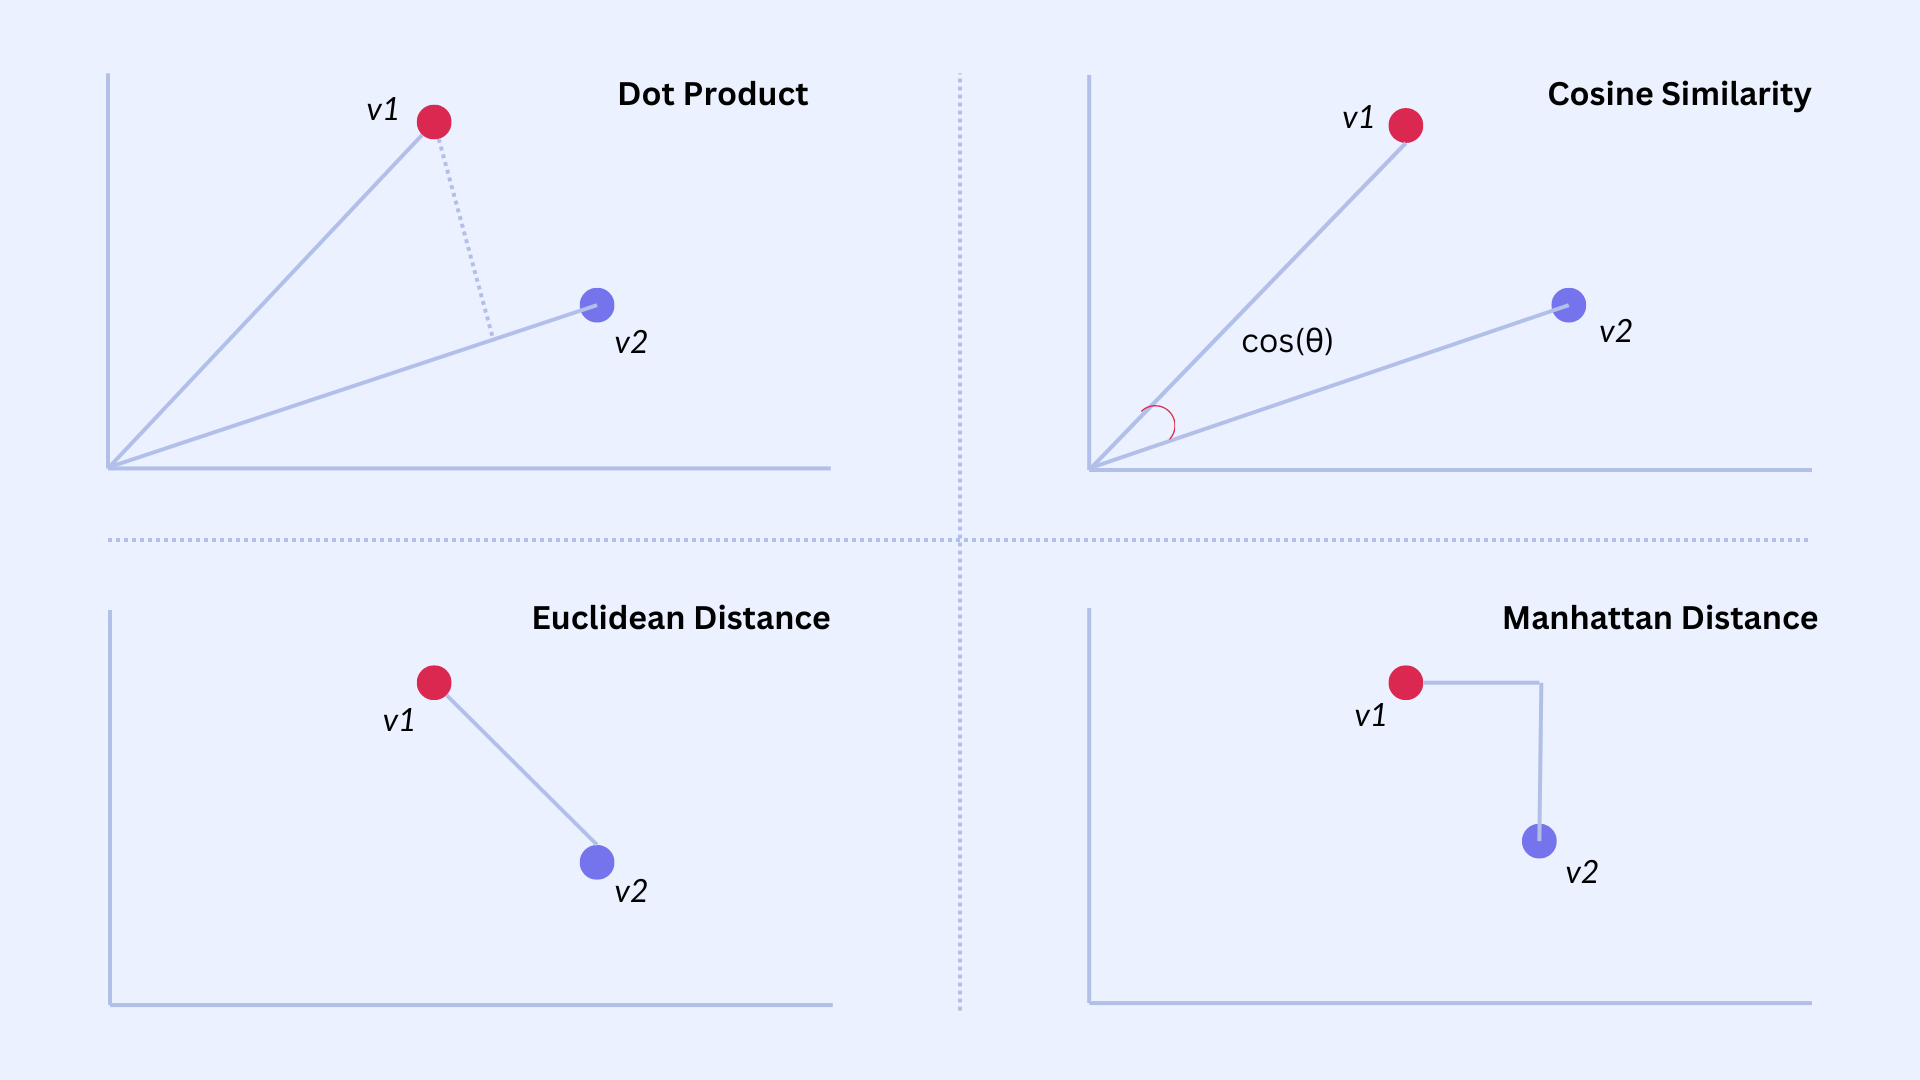
\includegraphics[width=0.75\linewidth]{Images/Kienthucnentang/vector-similarity.png}
    \caption[Vector Similarity trong semantic space với các vector embedding có ngữ nghĩa tương tự được phân bố gần nhau hơn trong không gian nhiều chiều]{Vector Similarity trong semantic space với các vector embedding có ngữ nghĩa tương tự được phân bố gần nhau hơn trong không gian nhiều chiều \cite{qdrant2024vectorsimilarity}}
    \label{fig:vector-similarity}
\end{figure}

\Cref{fig:vector-similarity}, vector similarity cho phép hệ thống xác định mức độ liên quan ngữ nghĩa giữa dữ liệu thông qua khoảng cách trong embedding space thay vì chỉ dựa trên keyword matching.
\subsubsection{Approximate Nearest Neighbor Search (ANN)}
Trong các hệ thống semantic search hiện đại, dữ liệu thường được biểu diễn dưới dạng vector embedding trong không gian nhiều chiều. Khi số lượng vector tăng lớn, việc tìm kiếm exact nearest neighbor trở nên tốn kém về thời gian và chi phí tính toán.

ANN là kỹ thuật tìm kiếm vector gần đúng nhằm tăng tốc quá trình retrieval trong không gian vector nhiều chiều \parencite{arya1998optimal}. Thay vì tìm vector gần nhất tuyệt đối, ANN chấp nhận kết quả gần đúng để đổi lấy thời gian truy xuất nhanh hơn.

ANN được sử dụng rộng rãi trong:
\begin{itemize}
    \item Semantic Search
    \item Vector Database
    \item Recommendation System
    \item Multimodal Retrieval
    \item Retrieval-Augmented Generation (RAG)
\end{itemize}

Các thuật toán ANN hiện đại như HNSW cho phép giảm đáng kể thời gian retrieval nhưng vẫn duy trì chất lượng tìm kiếm ở mức phù hợp cho semantic retrieval.

\begin{figure}[H]
    \centering
    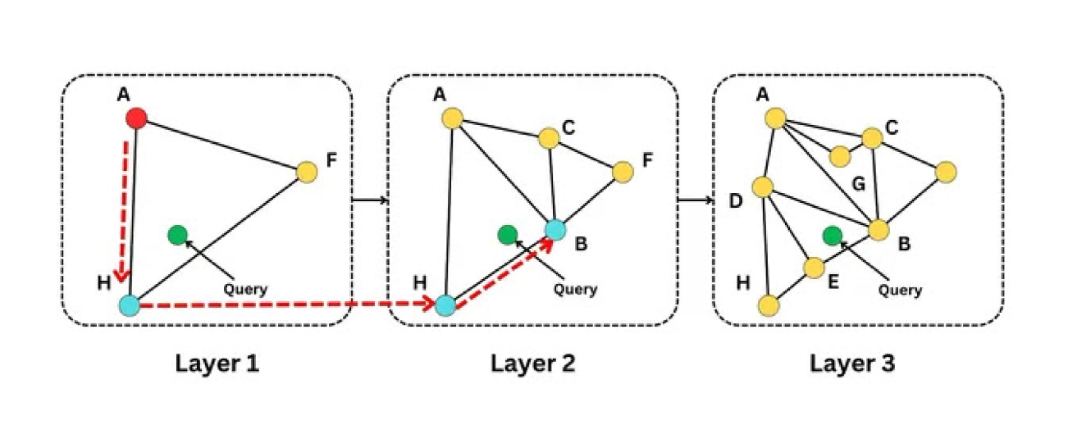
\includegraphics[width=1\linewidth]{Images/Kienthucnentang/ann-search-overview.png}
    \caption[Cơ chế Approximate Nearest Neighbor Search với quá trình truy xuất vector gần đúng nhằm tăng tốc tìm kiếm trong không gian vector nhiều chiều]{Cơ chế Approximate Nearest Neighbor Search với quá trình truy xuất vector gần đúng nhằm tăng tốc tìm kiếm trong không gian vector nhiều chiều \cite{analyticsvidhya2024ann}}
    \label{fig:ann-search-overview}
\end{figure}

\Cref{fig:ann-search-overview}, ANN search giúp hệ thống thực hiện vector retrieval hiệu quả trên tập dữ liệu lớn bằng cách giảm chi phí tìm kiếm trong không gian vector nhiều chiều.
\subsubsection{Hierarchical Navigable Small World (HNSW)}

HNSW là thuật toán Approximate Nearest Neighbor phổ biến trong các hệ thống semantic retrieval và vector database hiện đại \parencite{malkov2018efficient}.

HNSW xây dựng cấu trúc đồ thị nhiều tầng, trong đó mỗi node đại diện cho một vector embedding và các vector tương tự được kết nối với nhau. Quá trình tìm kiếm bắt đầu từ các tầng trên để nhanh chóng thu hẹp không gian tìm kiếm, sau đó tiếp tục refinement ở các tầng thấp hơn nhằm tìm nearest neighbor phù hợp.

Nhờ cơ chế tìm kiếm heuristic trên đồ thị phân tầng, HNSW giúp giảm đáng kể số lượng vector cần so sánh nhưng vẫn duy trì chất lượng retrieval cao.

Một số ưu điểm của HNSW gồm:
\begin{itemize}
    \item Tốc độ retrieval nhanh.
    \item Recall cao trong ANN search.
    \item Khả năng mở rộng tốt trên dữ liệu lớn.
\end{itemize}

Hiện nay, HNSW được sử dụng rộng rãi trong các vector database như Qdrant, Weaviate và Elasticsearch Vector Search.

\begin{figure}[H]
    \centering
    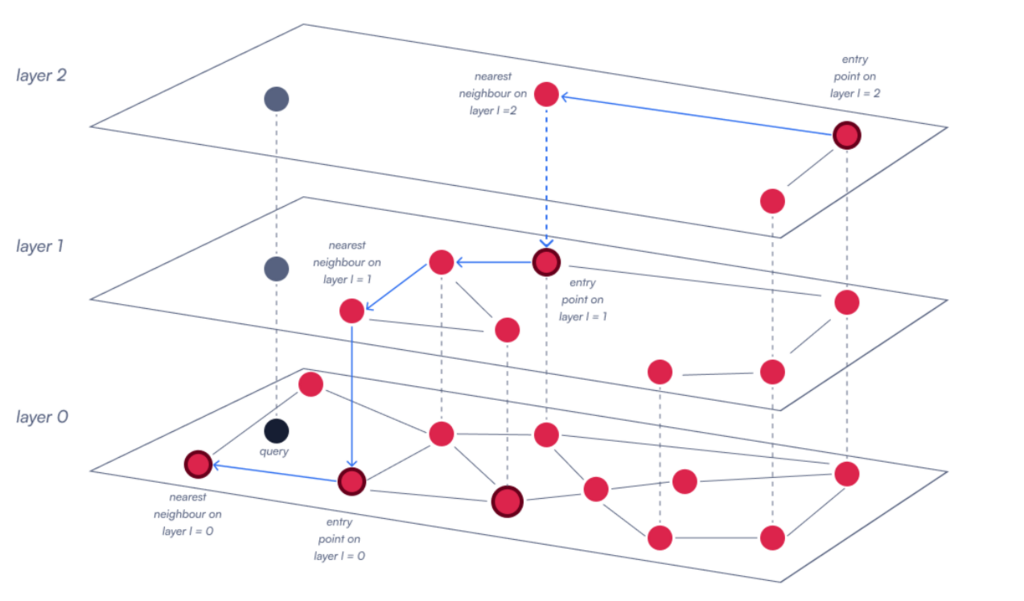
\includegraphics[width=0.75\linewidth]{Images/Kienthucnentang/hnsw-overview.png}
    \caption[Cấu trúc đồ thị phân tầng của thuật toán Hierarchical Navigable Small World (HNSW) trong Approximate Nearest Neighbor Search]{Cấu trúc đồ thị phân tầng của thuật toán Hierarchical Navigable Small World (HNSW) trong Approximate Nearest Neighbor Search \cite{qdrant2024hnsw}}
    \label{fig:hnsw-overview}
\end{figure}

\Cref{fig:hnsw-overview}, HNSW sử dụng cấu trúc đồ thị phân tầng để tăng tốc quá trình vector retrieval trong semantic search.

\subsection{Query Understanding và Query Processing}

\subsubsection{Query Understanding}

Query Understanding là quá trình phân tích truy vấn nhằm xác định ý định tìm kiếm và ngữ nghĩa của người dùng \parencite{guo2020deep}. Trong các hệ thống AI Search hiện đại, query understanding giúp hệ thống hiểu semantic meaning thay vì chỉ dựa trên keyword matching.

Trong thực tế, người dùng có thể sử dụng nhiều cách diễn đạt khác nhau cho cùng một nhu cầu tìm kiếm. Ví dụ, ``giày chạy bộ'', ``running shoes'' và ``sports sneakers'' có thể mang ý nghĩa tương tự dù khác từ vựng.

Mục tiêu của query understanding là chuyển đổi truy vấn thành semantic representation nhằm hỗ trợ retrieval và ranking hiệu quả hơn.

Một số thành phần chính của query understanding gồm:
\begin{itemize}
    \item Intent Understanding
    \item Semantic Representation
    \item Context Understanding
    \item Entity Recognition
\end{itemize}

Query understanding hiện được ứng dụng rộng rãi trong semantic search, recommendation system và conversational AI nhằm cải thiện chất lượng retrieval và độ liên quan của kết quả tìm kiếm.

\subsubsection{Query Expansion}

Query Expansion là kỹ thuật mở rộng truy vấn nhằm bổ sung các từ khóa hoặc biểu diễn ngữ nghĩa liên quan để cải thiện khả năng retrieval \parencite{carpineto2012survey}. Phương pháp này giúp hệ thống truy xuất dữ liệu hiệu quả hơn khi truy vấn ban đầu quá ngắn hoặc thiếu ngữ cảnh.

Một số hướng tiếp cận phổ biến gồm:

\begin{itemize}
    \item Synonym Expansion
    
    \item Semantic Expansion
    
    \item Knowledge-based Expansion
    
    \item Embedding-based Expansion
\end{itemize}

Ví dụ, truy vấn ``running shoes'' có thể được mở rộng thành ``sports sneakers'' hoặc ``giày chạy bộ'' nhằm tăng khả năng truy xuất các sản phẩm liên quan.

Query expansion hiện được sử dụng rộng rãi trong semantic search, recommendation system và conversational AI để cải thiện recall và semantic retrieval.

\subsubsection{Query Rewrite}

Query Rewrite là kỹ thuật chuyển đổi hoặc chuẩn hóa truy vấn nhằm tạo ra biểu diễn phù hợp hơn cho quá trình retrieval \parencite{ren2010query}. Phương pháp này giúp hệ thống xử lý các truy vấn viết tắt, sai chính tả hoặc diễn đạt không chuẩn nhưng vẫn giữ nguyên ý định tìm kiếm của người dùng.

Một số dạng query rewrite phổ biến gồm:

\begin{itemize}
    \item Spelling Correction
    
    \item Query Normalization
    
    \item Paraphrase Rewrite
    
    \item Context-aware Rewrite
\end{itemize}

Ví dụ, truy vấn ``nik running shose'' có thể được chuẩn hóa thành ``nike running shoes'' để cải thiện chất lượng retrieval.

Query rewrite hiện được sử dụng rộng rãi trong semantic search và conversational AI nhằm nâng cao khả năng hiểu truy vấn và semantic retrieval.

\subsubsection{Metadata Filtering}

Metadata Filtering là kỹ thuật lọc dữ liệu dựa trên các thuộc tính mô tả đi kèm với đối tượng trong quá trình retrieval. Phương pháp này cho phép hệ thống kết hợp tìm kiếm ngữ nghĩa với các điều kiện cụ thể như danh mục, thương hiệu, khoảng giá hoặc trạng thái còn hàng, từ đó giúp kết quả trả về phù hợp hơn với nhu cầu của người dùng.

Trong hệ thống E-commerce, metadata thường bao gồm các thông tin như danh mục sản phẩm, khoảng giá, thương hiệu, màu sắc, kích thước, trạng thái còn hàng hoặc thời gian tạo dữ liệu. Đây là các thuộc tính không nhất thiết phản ánh trực tiếp nội dung ngữ nghĩa của sản phẩm, nhưng lại đóng vai trò quan trọng trong việc giới hạn phạm vi tìm kiếm.

Metadata filtering có thể được triển khai dưới nhiều dạng khác nhau, chẳng hạn như lọc theo khoảng giá, lọc theo danh mục, lọc theo thuộc tính sản phẩm hoặc lọc theo điều kiện đúng sai. Ví dụ, với truy vấn ``nike running shoes under 2 million'', hệ thống có thể sử dụng semantic search để hiểu ý định tìm kiếm giày chạy bộ, đồng thời áp dụng metadata filtering để giới hạn kết quả theo thương hiệu Nike và mức giá dưới 2 triệu.

Trong các hệ thống AI Search, metadata filtering giúp kết quả truy xuất trở nên chính xác và phù hợp hơn với nhu cầu thực tế của người dùng. Thay vì chỉ trả về các sản phẩm có vector embedding gần với truy vấn, hệ thống còn có thể loại bỏ những sản phẩm không thỏa mãn điều kiện cụ thể như sai danh mục, vượt quá ngân sách hoặc không còn hàng.

Metadata filtering hiện được sử dụng rộng rãi trong vector database, recommendation system và semantic search nhằm hỗ trợ retrieval có điều kiện trên tập dữ liệu lớn.
% \subsubsection{Fusion Strategy}

% Fusion Strategy là kỹ thuật kết hợp nhiều nguồn thông tin hoặc nhiều tín hiệu retrieval nhằm cải thiện chất lượng kết quả tìm kiếm \parencite{vogt1999fusion}. Trong các hệ thống AI Search hiện đại, dữ liệu retrieval thường được sinh ra từ nhiều phương pháp khác nhau như keyword search, vector search hoặc metadata filtering.

% Mục tiêu của fusion strategy là tổng hợp các tín hiệu retrieval để tạo ra ranking cuối cùng có mức độ relevance cao hơn so với việc sử dụng riêng lẻ từng phương pháp.

% Một số hướng tiếp cận fusion phổ biến bao gồm:

% \begin{itemize}
%     \item \textbf{Score Fusion}: Kết hợp điểm số từ nhiều retrieval model.
    
%     \item \textbf{Rank Fusion}: Kết hợp thứ hạng từ nhiều danh sách retrieval.
    
%     \item \textbf{Weighted Fusion}: Gán trọng số cho từng nguồn tín hiệu retrieval.
    
%     \item \textbf{Multimodal Fusion}: Kết hợp thông tin từ nhiều modality khác nhau.
% \end{itemize}

% Fusion strategy giúp hệ thống tận dụng ưu điểm của nhiều phương pháp retrieval khác nhau nhằm nâng cao chất lượng semantic search và recommendation \parencite{wu2022multimodal}.

\subsection{Large Language Model và AI Agent}

\subsubsection{Khái niệm Large Language Model}

Large Language Model (LLM) là các mô hình học sâu có quy mô lớn, được huấn luyện trên lượng dữ liệu văn bản rất lớn nhằm học cách biểu diễn, hiểu và sinh ngôn ngữ tự nhiên. Các mô hình này thường được xây dựng dựa trên kiến trúc Transformer, trong đó cơ chế self-attention cho phép mô hình xác định mối quan hệ giữa các token trong câu và xử lý ngữ cảnh của văn bản đầu vào \parencite{vaswani2017attention}.

Khác với các mô hình xử lý ngôn ngữ truyền thống thường được thiết kế cho từng tác vụ cụ thể, LLM có khả năng thực hiện nhiều tác vụ khác nhau thông qua cùng một mô hình nền tảng. Người dùng có thể cung cấp yêu cầu dưới dạng prompt, sau đó mô hình sẽ sinh phản hồi dựa trên ngữ cảnh và tri thức đã học được trong quá trình huấn luyện.

LLM có thể được ứng dụng trong nhiều tác vụ xử lý ngôn ngữ tự nhiên như:

\begin{itemize}
    \item Sinh và xử lý văn bản: sinh văn bản tự động, tóm tắt văn bản, dịch máy.
    \item Hiểu và khai thác thông tin: trả lời câu hỏi, phân loại văn bản, trích xuất thông tin.
    \item Hỗ trợ tương tác thông minh: suy luận ngôn ngữ, chatbot và AI assistant.
\end{itemize}

Một số thành phần quan trọng trong LLM bao gồm tokenization, token embedding, positional encoding, self-attention, Transformer layer và language modeling head. Trong đó, tokenization giúp chia văn bản thành các đơn vị nhỏ hơn, embedding chuyển các token thành vector số, còn self-attention giúp mô hình nắm bắt quan hệ ngữ cảnh giữa các từ hoặc cụm từ trong chuỗi đầu vào.

Trong các hệ thống AI Search và AI Shopping Assistant, LLM có thể được sử dụng để hiểu ý định tìm kiếm của người dùng, diễn giải truy vấn tự nhiên, tạo câu trả lời hội thoại, hỗ trợ gợi ý sản phẩm và kết hợp với Retrieval-Augmented Generation (RAG) để sinh phản hồi dựa trên dữ liệu được truy xuất từ hệ thống.

\subsubsection{Prompt Engineering}
Prompt Engineering là kỹ thuật xây dựng và điều chỉnh prompt để định hướng Large Language Model tạo ra phản hồi phù hợp với mục tiêu của người dùng. Prompt có thể được xem là phần đầu vào mà người dùng hoặc hệ thống cung cấp cho mô hình, bao gồm yêu cầu nhiệm vụ, ngữ cảnh, ràng buộc xử lý và định dạng đầu ra mong muốn.

Chất lượng prompt có ảnh hưởng trực tiếp đến chất lượng phản hồi của LLM. Một prompt rõ ràng, đầy đủ ngữ cảnh và có cấu trúc tốt sẽ giúp mô hình hiểu đúng yêu cầu, giảm khả năng sinh kết quả sai lệch và tăng tính nhất quán của đầu ra. Ngược lại, prompt mơ hồ hoặc thiếu thông tin có thể khiến mô hình trả lời không đúng trọng tâm hoặc tạo ra kết quả không phù hợp với mục tiêu của hệ thống.

Một prompt hiệu quả thường bao gồm các thành phần chính sau:

\begin{itemize}
    \item \textbf{Nội dung hướng dẫn}: bao gồm instruction, context và constraint, giúp mô hình hiểu nhiệm vụ, dữ liệu liên quan và các giới hạn cần tuân theo.
    \item \textbf{Định dạng và ví dụ}: bao gồm output format và example, giúp mô hình tạo đầu ra đúng cấu trúc và phù hợp với mong muốn của người dùng.
\end{itemize}

Một số dạng prompting phổ biến gồm:

\begin{itemize}
    \item \textbf{Zero-shot và Few-shot Prompting}: zero-shot không cung cấp ví dụ mẫu, còn few-shot cung cấp một vài ví dụ đầu vào và đầu ra để mô hình phản hồi theo mẫu.
    \item \textbf{Instruction và Chain-of-Thought Prompting}: instruction prompting sử dụng hướng dẫn rõ ràng, còn chain-of-thought prompting khuyến khích mô hình trình bày các bước suy luận trước khi đưa ra kết quả cuối cùng.
\end{itemize}

Trong các hệ thống E-commerce, Prompt Engineering có thể được sử dụng để điều khiển cách AI assistant trả lời người dùng, diễn giải truy vấn tìm kiếm, trích xuất thuộc tính sản phẩm, tạo mô tả sản phẩm hoặc sinh câu trả lời dựa trên kết quả truy xuất. Ví dụ, với truy vấn ``tìm laptop cho sinh viên học lập trình giá dưới 20 triệu'', prompt có thể hướng dẫn LLM xác định các tiêu chí như mục đích sử dụng, khoảng giá, hiệu năng, dung lượng RAM và mức độ phù hợp của từng sản phẩm.

Prompt Engineering hiện được sử dụng rộng rãi trong chatbot, AI assistant, hệ thống hỏi đáp, hệ thống tìm kiếm thông minh và các ứng dụng reasoning dựa trên LLM.

\subsubsection{Function Calling}

Function Calling là cơ chế cho phép Large Language Model kết nối và sử dụng các hàm, API hoặc công cụ bên ngoài để mở rộng khả năng xử lý. Thay vì chỉ sinh văn bản từ tri thức đã học, mô hình có thể xác định khi nào cần gọi công cụ, truyền tham số phù hợp và sử dụng kết quả trả về để tạo phản hồi cuối cùng cho người dùng.

Cơ chế này đặc biệt hữu ích trong các bài toán yêu cầu dữ liệu động hoặc thao tác với hệ thống bên ngoài. Ví dụ, LLM có thể gọi API để tra cứu thông tin sản phẩm, kiểm tra tồn kho, lấy giá hiện tại, truy vấn cơ sở dữ liệu, tạo đơn hàng hoặc lọc danh sách sản phẩm theo điều kiện cụ thể.

Một hệ thống Function Calling thường bao gồm các thành phần chính sau:

\begin{itemize}
    \item \textbf{Function Schema}: Mô tả tên hàm, mục đích sử dụng, danh sách tham số và kiểu dữ liệu đầu vào.
    \item \textbf{Tool Selection}: Quá trình mô hình xác định công cụ hoặc hàm phù hợp với yêu cầu của người dùng.
    \item \textbf{Tool Invocation}: Quá trình gọi hàm với các tham số được mô hình suy luận từ prompt.
    \item \textbf{Structured Output}: Kết quả được trả về dưới dạng có cấu trúc, giúp hệ thống dễ xử lý và kiểm tra.
    \item \textbf{Result Integration}: Kết hợp kết quả từ công cụ bên ngoài vào phản hồi cuối cùng của LLM.
\end{itemize}

Trong AI Shopping Assistant, Function Calling có thể được sử dụng để kết nối LLM với các dịch vụ nội bộ của hệ thống E-commerce. Khi người dùng đưa ra yêu cầu như ``tìm điện thoại dưới 10 triệu có pin tốt'', LLM có thể phân tích yêu cầu, gọi hàm tìm kiếm sản phẩm với các tham số như danh mục, khoảng giá và tiêu chí pin, sau đó tổng hợp kết quả để đưa ra gợi ý phù hợp.

Function Calling giúp LLM trở nên đáng tin cậy hơn trong các tác vụ cần dữ liệu chính xác và cập nhật, vì mô hình không cần tự suy đoán toàn bộ thông tin. Thay vào đó, mô hình có thể phối hợp với cơ sở dữ liệu, search engine, recommendation engine hoặc các API nghiệp vụ để tạo ra phản hồi có căn cứ hơn.

Nhờ khả năng kết nối giữa ngôn ngữ tự nhiên và các chức năng hệ thống, Function Calling hiện được sử dụng rộng rãi trong chatbot, AI assistant, AI agent và các hệ thống tự động hóa nhiều bước.

\subsubsection{Khái niệm AI Agent}

AI Agent là hệ thống trí tuệ nhân tạo có khả năng tiếp nhận thông tin, phân tích ngữ cảnh, thực hiện reasoning và đưa ra hành động nhằm đạt được một mục tiêu cụ thể \parencite{wooldridge2009introduction}. Khác với chatbot truyền thống chủ yếu phản hồi theo từng lượt hội thoại, AI Agent có thể tương tác với công cụ, dữ liệu hoặc môi trường bên ngoài để xử lý các tác vụ phức tạp hơn.

Một AI Agent thường bao gồm bốn thành phần chính: perception, reasoning, memory và action. Trong đó, perception giúp agent tiếp nhận thông tin đầu vào, reasoning hỗ trợ phân tích và lựa chọn hướng xử lý, memory lưu trữ ngữ cảnh hoặc lịch sử tương tác, còn action cho phép agent thực hiện hành động như gọi API, truy xuất dữ liệu hoặc tạo phản hồi cho người dùng.

Trong hệ thống AI Shopping Assistant, AI Agent có thể hỗ trợ người dùng tìm kiếm sản phẩm, lọc kết quả theo nhu cầu, so sánh sản phẩm và đưa ra gợi ý phù hợp. Nhờ khả năng kết hợp giữa hiểu ngôn ngữ tự nhiên và sử dụng công cụ bên ngoài, AI Agent được ứng dụng rộng rãi trong conversational AI, recommendation system và các hệ thống trợ lý thông minh.
\subsection{Retrieval-Augmented Generation (RAG)}
\subsubsection{Khái niệm RAG}

Retrieval-Augmented Generation (RAG) là kiến trúc kết hợp giữa khả năng truy xuất thông tin và khả năng sinh ngôn ngữ của Large Language Model nhằm hỗ trợ tạo ra phản hồi có độ chính xác và tính cập nhật cao hơn \parencite{lewis2020rag}.

Trong các mô hình ngôn ngữ truyền thống, tri thức chủ yếu được lưu trữ trong tham số của mô hình sau quá trình huấn luyện. Tuy nhiên, các mô hình này thường gặp hạn chế về khả năng cập nhật kiến thức mới hoặc truy xuất thông tin chuyên biệt theo từng miền dữ liệu. RAG được đề xuất nhằm giải quyết vấn đề này bằng cách cho phép hệ thống truy xuất thêm dữ liệu từ nguồn tri thức bên ngoài trước khi sinh phản hồi.

Về mặt nguyên lý, RAG hoạt động bằng cách kết hợp truy vấn của người dùng với các tài liệu liên quan được truy xuất từ knowledge base. Các tài liệu này đóng vai trò context bổ sung cho mô hình ngôn ngữ trong quá trình sinh câu trả lời.

RAG hiện được sử dụng rộng rãi trong nhiều hệ thống AI hiện đại như semantic search, chatbot, AI assistant và question answering system nhờ khả năng:
\begin{itemize}
    \item Giảm hiện tượng hallucination
    
    \item Tăng khả năng grounding vào dữ liệu thực tế
    
    \item Hỗ trợ truy xuất tri thức quy mô lớn
    
    \item Cải thiện độ chính xác của phản hồi
\end{itemize}

\subsubsection{Kiến trúc RAG}

Kiến trúc RAG thường bao gồm hai thành phần chính là retrieval module và generation module.

\begin{itemize}
    \item \textbf{Retrieval Module}: Thành phần chịu trách nhiệm truy xuất các tài liệu liên quan từ kho tri thức.
    
    \item \textbf{Generation Module}: Thành phần sử dụng thông tin truy xuất được để sinh phản hồi ngôn ngữ tự nhiên.
\end{itemize}

Trong quy trình hoạt động của RAG, truy vấn đầu vào trước tiên được chuyển đổi thành semantic representation thông qua embedding model. Sau đó, hệ thống thực hiện retrieval trên vector database hoặc knowledge base để tìm các tài liệu có mức độ liên quan cao. Các tài liệu này sẽ được kết hợp với truy vấn ban đầu và đưa vào mô hình ngôn ngữ để sinh câu trả lời cuối cùng.
\begin{figure}[H]
    \centering
    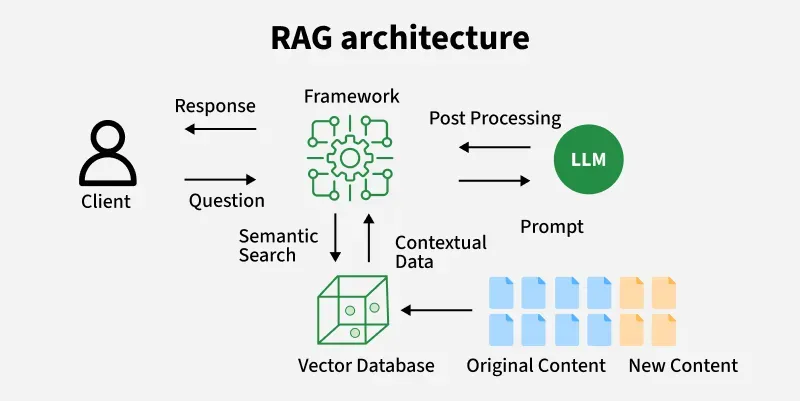
\includegraphics[width=0.75\textwidth]{Images/Kienthucnentang/RAG-architecture.png}
    \caption[Minh họa kiến trúc Retrieval-Augmented Generation (RAG)]{Minh họa kiến trúc Retrieval-Augmented Generation (RAG) \parencite{geeksforgeeks2026ragarchitecture}}
    \label{fig:rag-architecture}
\end{figure}
Kiến trúc RAG giúp hệ thống kết hợp đồng thời:
\begin{itemize}
    \item Khả năng semantic retrieval
    
    \item Khả năng reasoning của LLM
    
    \item Khả năng sinh ngôn ngữ tự nhiên
\end{itemize}

Nhờ đó, RAG có thể hỗ trợ xử lý hiệu quả các bài toán yêu cầu truy xuất tri thức động hoặc dữ liệu chuyên biệt theo từng miền ứng dụng.

\subsubsection{Retriever và Generator}
Trong kiến trúc RAG, retriever và generator là hai thành phần cốt lõi ảnh hưởng trực tiếp đến chất lượng phản hồi của hệ thống. Retriever chịu trách nhiệm tìm kiếm và truy xuất các tài liệu liên quan, trong khi generator sử dụng thông tin được truy xuất để tạo ra câu trả lời cuối cùng.

Retriever là thành phần thực hiện truy xuất dữ liệu liên quan từ knowledge base hoặc vector database dựa trên truy vấn đầu vào. Trong các hệ thống semantic retrieval hiện đại, retriever thường sử dụng dense vector retrieval nhằm tìm kiếm dữ liệu dựa trên semantic similarity thay vì keyword matching truyền thống.

Một số nhiệm vụ chính của retriever bao gồm:
\begin{itemize}
    \item Biểu diễn truy vấn dưới dạng vector embedding
    
    \item Tìm kiếm các tài liệu liên quan
    
    \item Tối ưu recall trong quá trình retrieval
\end{itemize}

Generator là thành phần chịu trách nhiệm sinh phản hồi cuối cùng dựa trên truy vấn và các tài liệu được retriever cung cấp. Generator thường là Large Language Model với khả năng tổng hợp thông tin và sinh ngôn ngữ tự nhiên.

Generator có vai trò:
\begin{itemize}
    \item Tổng hợp thông tin từ nhiều nguồn
    
    \item Thực hiện reasoning trên context truy xuất
    
    \item Sinh phản hồi tự nhiên và mạch lạc
\end{itemize}

Sự kết hợp giữa retriever và generator giúp hệ thống vừa có khả năng truy xuất thông tin chính xác vừa đảm bảo chất lượng phản hồi ngôn ngữ tự nhiên.

\subsubsection{Conversation Memory}

Conversation Memory là cơ chế giúp hệ thống conversational AI lưu trữ và duy trì ngữ cảnh trong quá trình hội thoại. Nhờ cơ chế này, hệ thống có thể ghi nhớ nội dung đã trao đổi trước đó và tạo ra phản hồi nhất quán hơn trong các cuộc hội thoại nhiều lượt.

Trong thực tế, truy vấn hiện tại của người dùng thường phụ thuộc vào các lượt hội thoại trước. Ví dụ, người dùng có thể hỏi ``sản phẩm này có rẻ hơn không'' sau khi vừa xem một danh sách sản phẩm. Nếu không có memory, hệ thống sẽ khó xác định người dùng đang nhắc đến sản phẩm nào.

Conversation Memory có thể được triển khai dưới nhiều dạng như lịch sử hội thoại, bản tóm tắt ngữ cảnh, context embedding hoặc bộ nhớ ngoài lưu trong cơ sở dữ liệu. Trong các hệ thống RAG, memory thường được kết hợp với retrieval mechanism để truy xuất thông tin theo ngữ cảnh, từ đó cải thiện khả năng reasoning và chất lượng phản hồi.

\subsubsection{Agentic RAG}

Agentic RAG là hướng mở rộng của Retrieval-Augmented Generation, trong đó mô hình ngôn ngữ không chỉ thực hiện truy xuất và sinh phản hồi theo một pipeline cố định, mà còn hoạt động như một AI agent có khả năng reasoning, lựa chọn hành động và sử dụng công cụ trong quá trình xử lý truy vấn \parencite{yao2023react}.

Khác với RAG truyền thống có pipeline tương đối cố định, Agentic RAG cho phép hệ thống linh hoạt quyết định khi nào cần truy xuất thông tin, khi nào cần suy luận, khi nào cần gọi external tools và khi nào sinh phản hồi cuối cùng. Quá trình xử lý có thể diễn ra theo nhiều vòng lặp giữa retrieve, reason và generate để từng bước hoàn thiện câu trả lời.

Một số đặc điểm nổi bật của Agentic RAG gồm multi-step reasoning, dynamic retrieval, tool usage integration và adaptive decision making. Nhờ các đặc điểm này, hệ thống có thể xử lý tốt hơn các truy vấn phức tạp, truy vấn nhiều điều kiện hoặc các tác vụ yêu cầu reasoning đa bước.

Trong hệ thống AI Shopping Assistant, Agentic RAG có thể hỗ trợ các yêu cầu như tìm kiếm sản phẩm theo nhiều tiêu chí, so sánh sản phẩm, lọc theo ngân sách, kiểm tra tồn kho hoặc giải thích lý do đề xuất. Vì vậy, Agentic RAG là hướng tiếp cận quan trọng trong các hệ thống AI assistant hiện đại nhờ khả năng kết hợp retrieval, reasoning và hành động trong cùng một quy trình xử lý.
\subsection*{Kết chương}

Chương này đã trình bày các kiến thức nền tảng phục vụ cho việc xây dựng hệ thống tìm kiếm thông minh trong thương mại điện tử. Nội dung chương bao gồm bài toán tìm kiếm sản phẩm, hạn chế của keyword-based search, semantic search, multimodal search và vai trò của AI trong việc cải thiện chất lượng tìm kiếm.

Bên cạnh đó, chương đã giới thiệu các nền tảng quan trọng của hệ thống truy hồi thông tin như BM25, semantic retrieval, vector embedding, vector similarity, vector database, ANN và HNSW. Đây là các thành phần giúp hệ thống biểu diễn dữ liệu dưới dạng vector và truy xuất kết quả phù hợp trong không gian ngữ nghĩa.

Chương cũng trình bày các kỹ thuật xử lý truy vấn như query understanding, query expansion, query rewrite và metadata filtering nhằm nâng cao độ chính xác của kết quả retrieval. Ngoài ra, các nội dung về Computer Vision, Text-Image Retrieval và Object Detection làm rõ cách hệ thống khai thác dữ liệu hình ảnh trong tìm kiếm sản phẩm.

Cuối cùng, chương đã giới thiệu các khái niệm về Large Language Model, AI Agent và Retrieval-Augmented Generation, bao gồm prompt engineering, function calling, conversation memory và Agentic RAG. Những kiến thức này là cơ sở để thiết kế hệ thống AI Shopping Assistant có khả năng hiểu truy vấn, truy xuất dữ liệu, suy luận và sinh phản hồi tự nhiên trong các chương tiếp theo.
%=========================
% Sections/03-CongTrinhLienQuan.tex
% Chương 3 – Các công trình liên quan
%=========================
\section{Công nghệ liên quan}
\subsection{Các mô hình kiến trúc phần mềm}

Kiến trúc hệ thống là một trong những yếu tố quan trọng quyết định khả năng mở rộng, hiệu năng và tính linh hoạt của hệ thống phần mềm. Kiến trúc phần mềm mô tả cấu trúc tổng thể của hệ thống, bao gồm các thành phần chính, mối quan hệ giữa các thành phần và cách chúng tương tác với nhau trong quá trình xử lý dữ liệu.

Trong các hệ thống hiện đại, đặc biệt là hệ thống trí tuệ nhân tạo trong lĩnh vực thương mại điện tử, kiến trúc hệ thống cần hỗ trợ xử lý phân tán, tích hợp nhiều dịch vụ AI và đảm bảo khả năng mở rộng linh hoạt theo tải hệ thống. Các mô hình kiến trúc phổ biến hiện nay bao gồm monolithic architecture, microservice architecture và cloud-native architecture.

%=========================
\subsubsection{Monolithic Architecture}

Monolithic architecture là mô hình kiến trúc trong đó toàn bộ hệ thống được xây dựng và triển khai như một khối thống nhất. Các thành phần như giao diện người dùng, logic nghiệp vụ và tầng truy cập dữ liệu thường nằm trong cùng một ứng dụng, chia sẻ chung mã nguồn, môi trường chạy và quy trình triển khai.

Như trình bày ở \Cref{fig:monolithic_architecture}, toàn bộ hệ thống được triển khai trong một khối thống nhất.

\begin{figure}[H]
    \centering
    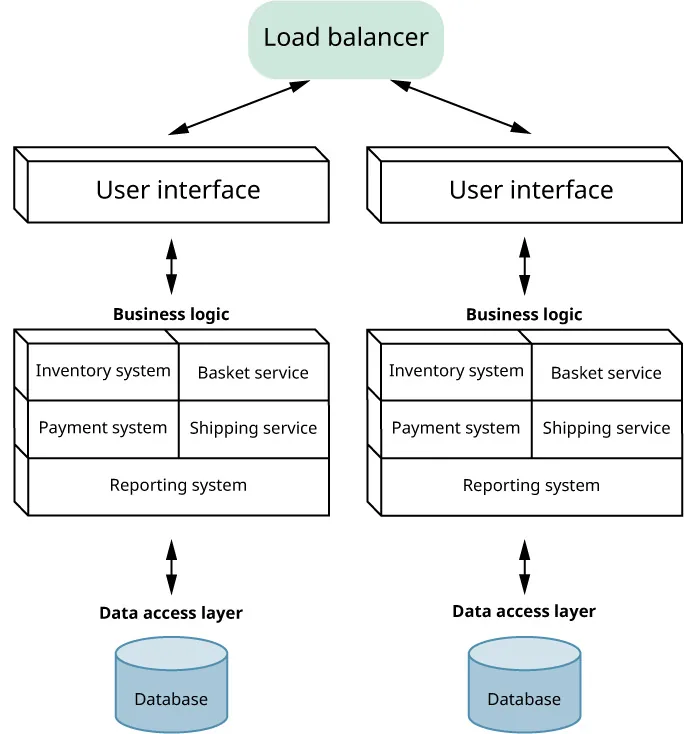
\includegraphics[width=0.5\textwidth]{Images/Congnghelienquan/Monolithic_architecture.png}
    \caption[Kiến trúc monolithic trong đó toàn bộ thành phần hệ thống được triển khai trong một ứng dụng duy nhất (nguồn: OpenStax)]{Kiến trúc monolithic trong đó toàn bộ thành phần hệ thống được triển khai trong một ứng dụng duy nhất (nguồn: OpenStax \parencite{openstax_cloud_native_intro})}
    \label{fig:monolithic_architecture}
\end{figure}

Trong kiến trúc monolithic, toàn bộ hệ thống thường nằm trong một codebase duy nhất, các module chia sẻ chung tài nguyên và giao tiếp nội bộ trong cùng tiến trình. Cách tổ chức này giúp việc phát triển, kiểm thử và triển khai ban đầu trở nên đơn giản, đặc biệt phù hợp với các hệ thống nhỏ hoặc các phiên bản thử nghiệm ban đầu.

Ưu điểm của monolithic architecture là cấu trúc dễ hiểu, ít phức tạp trong triển khai và có hiệu năng tốt do không phát sinh overhead mạng giữa các thành phần. Tuy nhiên, khi hệ thống phát triển lớn hơn, kiến trúc này có thể gặp khó khăn trong việc mở rộng, bảo trì và cập nhật từng chức năng riêng lẻ. Sự phụ thuộc chặt giữa các module cũng khiến việc thay đổi một thành phần có thể ảnh hưởng đến toàn bộ hệ thống.

%=========================
\subsubsection{Microservice Architecture}

Microservice architecture là mô hình kiến trúc trong đó hệ thống được chia thành nhiều dịch vụ nhỏ, độc lập và giao tiếp với nhau thông qua API. Mỗi service thường đảm nhiệm một chức năng nghiệp vụ riêng, có thể được phát triển, kiểm thử, triển khai và mở rộng độc lập với các service khác.

Như trình bày ở \Cref{fig:microservice_architecture}, hệ thống được phân tách thành các service độc lập.

\begin{figure}[H]
    \centering
    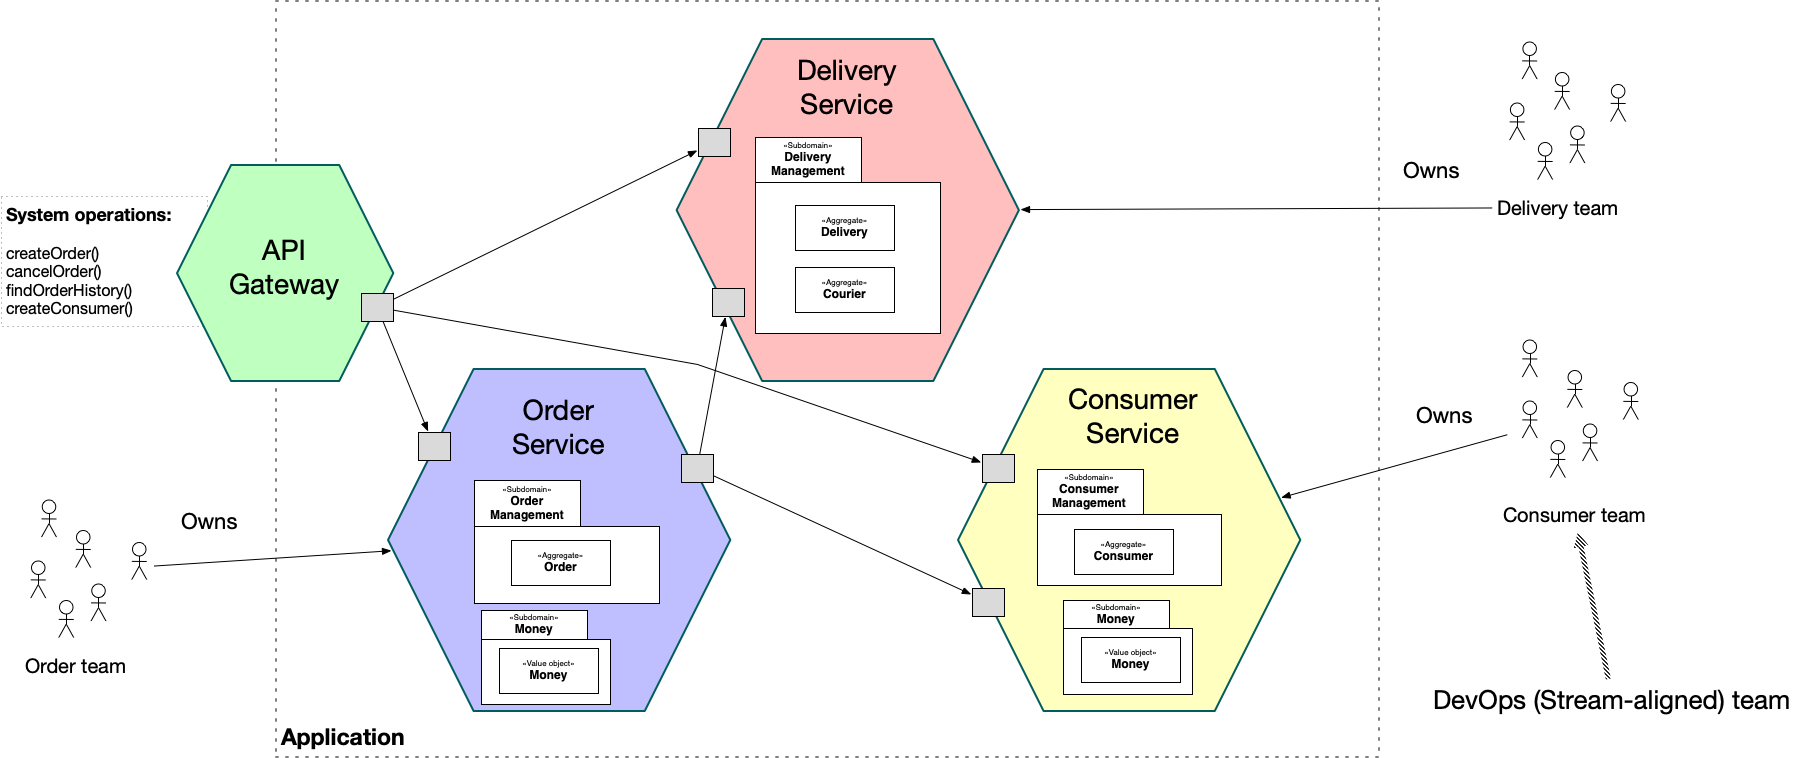
\includegraphics[width=0.85\textwidth]{Images/Congnghelienquan/microservices-teams-subdomains.png}
    \caption[Kiến trúc microservice trong đó hệ thống được chia thành các dịch vụ nhỏ, độc lập và giao tiếp qua API (nguồn: Microservices.io)]{Kiến trúc microservice trong đó hệ thống được chia thành các dịch vụ nhỏ, độc lập và giao tiếp qua API (nguồn: Microservices.io \parencite{microservices_io_patterns})}
    \label{fig:microservice_architecture}
\end{figure}

Trong kiến trúc microservice, hệ thống được tổ chức thành nhiều service độc lập, mỗi service phụ trách một nhóm chức năng cụ thể và giao tiếp với nhau thông qua REST API, gRPC hoặc message broker. Các service có thể được phát triển bằng công nghệ khác nhau tùy theo yêu cầu nghiệp vụ, miễn là chúng tuân thủ cơ chế giao tiếp đã được thiết kế.

Ưu điểm của microservice architecture là khả năng mở rộng linh hoạt theo từng thành phần, hỗ trợ phát triển song song giữa các nhóm và tăng khả năng chịu lỗi của hệ thống. Khi một service gặp sự cố, các service khác vẫn có thể tiếp tục hoạt động nếu hệ thống được thiết kế tốt.

Tuy nhiên, microservice cũng làm tăng độ phức tạp trong vận hành vì hệ thống trở thành một môi trường phân tán. Việc triển khai, monitoring, logging, tracing và orchestration cần được quản lý chặt chẽ. Ngoài ra, giao tiếp giữa các service có thể phát sinh overhead mạng và làm tăng độ trễ so với kiến trúc monolithic.
%=========================
\subsubsection{Service-based Architecture}

Service-based architecture là mô hình kiến trúc trong đó hệ thống được chia thành nhiều service độc lập theo từng nhóm chức năng hoặc nghiệp vụ. Mỗi service đảm nhiệm một vai trò cụ thể và giao tiếp với các service khác thông qua API. Cách tiếp cận này giúp hệ thống dễ mở rộng, dễ bảo trì và phù hợp với các hệ thống có nhiều thành phần xử lý riêng biệt như tìm kiếm, gợi ý sản phẩm, quản lý người dùng và xử lý AI.

Khác với monolithic architecture, service-based architecture không gom toàn bộ chức năng vào một ứng dụng duy nhất. Thay vào đó, hệ thống được tổ chức thành các service có trách nhiệm rõ ràng. Tuy nhiên, mô hình này không nhất thiết phải tách nhỏ đến mức microservices hoàn chỉnh, mà có thể chia theo các module lớn hơn để giảm độ phức tạp trong triển khai.

Như trình bày ở \Cref{fig:service_based_architecture}, hệ thống service-based được tổ chức thành nhiều service độc lập và giao tiếp với nhau thông qua API.

\begin{figure}[H]
    \centering
    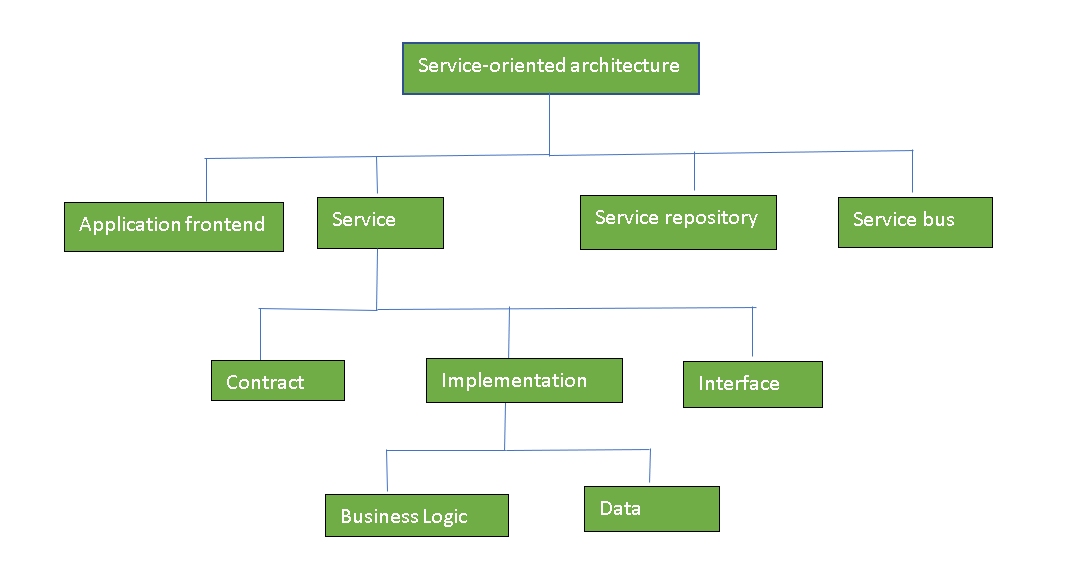
\includegraphics[width=0.85\textwidth]{Images/Congnghelienquan/service-base-architectural.png}
    \caption[Kiến trúc service-based chia hệ thống thành nhiều service độc lập và giao tiếp thông qua API]{Kiến trúc service-based chia hệ thống thành nhiều service độc lập và giao tiếp thông qua API \parencite{geeksforgeeks2023soa}}
    \label{fig:service_based_architecture}
\end{figure}

Trong service-based architecture, hệ thống được chia thành các service theo chức năng, mỗi service có thể được phát triển, bảo trì và mở rộng tương đối độc lập. Các service giao tiếp với nhau thông qua API, giúp giảm sự phụ thuộc trực tiếp giữa các module so với monolithic architecture.

Ưu điểm của kiến trúc này là dễ mở rộng từng thành phần, dễ thay đổi hoặc nâng cấp một service mà không ảnh hưởng quá nhiều đến toàn bộ hệ thống. Mô hình này cũng phù hợp với các hệ thống có nhiều thành phần riêng biệt như search service, recommendation service, user service, LLM service và vector database service.

Tuy nhiên, service-based architecture yêu cầu thiết kế API rõ ràng giữa các service. Việc quản lý giao tiếp, đồng bộ dữ liệu và xử lý lỗi giữa các service cũng phức tạp hơn so với monolithic architecture. Ngoài ra, hệ thống có thể phát sinh độ trễ khi các service gọi nhau thông qua mạng.

%=========================
\subsubsection{So sánh kiến trúc hệ thống}

Như tổng hợp ở Bảng \Cref{tab:architecture_comparison}, các kiến trúc được so sánh dựa trên khả năng mở rộng, mức độ triển khai, bảo trì và sự phù hợp với hệ thống AI.

\begin{table}[H]
\centering
\caption{So sánh các kiến trúc hệ thống phổ biến trong ứng dụng AI hiện đại}
\label{tab:architecture_comparison}
\renewcommand{\arraystretch}{1.3}

\begin{tabularx}{\linewidth}{|>{\raggedright\arraybackslash}X|>{\raggedright\arraybackslash}X|>{\raggedright\arraybackslash}X|>{\raggedright\arraybackslash}X|}
\hline
\textbf{Tiêu chí} & \textbf{Monolithic} & \textbf{Microservice} & \textbf{Service-based} \\ \hline
Khả năng mở rộng & Thấp & Cao & Rất cao \\ \hline
Triển khai & Đơn giản & Trung bình & Phức tạp \\ \hline
Bảo trì & Khó & Dễ & Dễ hơn monolithic \\ \hline
Hiệu năng & Tốt (nhỏ) & Ổn định & Tối ưu cho các service lớn \\ \hline
Phù hợp AI system & Thấp & Cao & Rất cao \\ \hline
\end{tabularx}
\end{table}

Tổng kết lại, kiến trúc microservice và service-based là lựa chọn phù hợp cho các hệ thống AI hiện đại nhờ khả năng mở rộng linh hoạt, hỗ trợ triển khai phân tán và tích hợp tốt với các thành phần như vector database, embedding models và các dịch vụ AI.
%=========================
\subsection{Backend Framework}
\subsubsection{ASP.NET Core (.NET)}

ASP.NET Core là framework xây dựng ứng dụng web và API trong hệ sinh thái .NET, sử dụng ngôn ngữ C\# và hỗ trợ triển khai đa nền tảng \parencite{ch4_aspnet_overview}. Framework cung cấp middleware, dependency injection, xác thực và phân quyền để tổ chức xử lý yêu cầu và nghiệp vụ.

Trong Wispace, ASP.NET Core được lựa chọn để xây dựng các dịch vụ Core, Learning \& Exam, Assessment và Progress \& Reporting. AIHub sử dụng backend ASP.NET Core riêng theo modular monolith, phục vụ quản lý tổ chức, khóa API, hạn mức và các công cụ học thuật nội bộ. Các tác vụ suy luận được tách sang dịch vụ Python FastAPI.

\textbf{Ứng dụng trong hệ thống:}
\begin{itemize}
    \item Xây dựng API cho luyện tập, thi thử, kết quả và quản trị Wispace.
    \item Quản lý tổ chức, quyền truy cập API và usage của AIHub.
    \item Truy cập PostgreSQL qua EF Core và Npgsql; schema được quản lý riêng bằng Flyway và SQL migration.
    \item Điều phối công việc nền qua RabbitMQ và gọi dịch vụ AI bằng HTTP.
\end{itemize}

%=========================

\subsubsection{FastAPI}

FastAPI là framework Python dùng để xây dựng API theo chuẩn ASGI, hỗ trợ lập trình bất đồng bộ, kiểm tra dữ liệu dựa trên khai báo kiểu và tự động sinh tài liệu OpenAPI \parencite{fastapidocs2024}. Framework phù hợp để cung cấp giao diện gọi mô hình AI và tích hợp các thư viện xử lý tiếng nói, học máy trong Python.

Trong Wispace, FastAPI cung cấp API cho pipeline chấm Speaking gồm M5 xử lý âm học, M6 đánh giá ngôn ngữ và M7 tổng hợp kết quả. Đối với AIHub, FastAPI cung cấp giao diện thực thi dịch vụ mô hình và sinh nội dung học thuật. Backend ASP.NET Core quản lý nghiệp vụ, quyền truy cập và hạn mức trước khi gọi dịch vụ AI.

\textbf{Ứng dụng trong hệ thống:}
\begin{itemize}
    \item Tiếp nhận audio và ngữ cảnh câu hỏi để thực thi pipeline chấm Speaking.
    \item Kiểm tra dữ liệu đầu vào, trả điểm và nhận xét theo hợp đồng API thống nhất.
    \item Cung cấp API cho các tác vụ AI của AIHub, tách xử lý mô hình khỏi backend nghiệp vụ.
\end{itemize}

%=========================

\subsubsection{Node.js}

Node.js là môi trường runtime JavaScript được xây dựng trên V8 engine của Google Chrome nhằm hỗ trợ phát triển ứng dụng phía server \parencite{nodejsdocs2024}. Node.js sử dụng mô hình event-driven và non-blocking I/O giúp tối ưu khả năng xử lý đồng thời và giảm chi phí tài nguyên trong các hệ thống có lượng request lớn.

Khác với các kiến trúc xử lý đồng bộ truyền thống, Node.js cho phép hệ thống xử lý nhiều kết nối đồng thời thông qua cơ chế asynchronous programming. Điều này giúp Node.js phù hợp với các ứng dụng realtime hoặc các dịch vụ cần phản hồi nhanh.

Trong các hệ thống backend hiện đại, Node.js thường được sử dụng cho các thành phần realtime hoặc lightweight service.

%=========================
\subsubsection{So sánh Backend Framework}

Nhằm làm rõ sự khác biệt giữa các backend framework, Bảng \Cref{tab:backend_framework} tổng hợp so sánh dựa trên các tiêu chí quan trọng như hiệu năng, khả năng hỗ trợ AI và mức độ phù hợp với hệ thống phân tán.

\begin{table}[H]
\centering
\caption{So sánh các backend framework phổ biến dựa trên hiệu năng, khả năng hỗ trợ AI và mức độ phù hợp với kiến trúc hệ thống phân tán}
\label{tab:backend_framework}
\renewcommand{\arraystretch}{1.3}

\begin{tabularx}{\linewidth}{|>{\raggedright\arraybackslash}X|>{\raggedright\arraybackslash}X|>{\raggedright\arraybackslash}X|>{\raggedright\arraybackslash}X|}
\hline
\textbf{Tiêu chí} & \textbf{ASP.NET Core} & \textbf{FastAPI} & \textbf{Node.js} \\ \hline
Ngôn ngữ & C\# & Python & JavaScript \\ \hline
Hiệu năng & Cao & Rất cao & Cao \\ \hline
Hỗ trợ AI/ML & Trung bình & Rất tốt & Thấp \\ \hline
Microservices & Rất tốt & Tốt & Tốt \\ \hline
Realtime & Tốt & Trung bình & Rất tốt \\ \hline
Ứng dụng phù hợp & Enterprise backend & AI services & Realtime systems \\ \hline
\end{tabularx}
\end{table}

Wispace và AIHub kết hợp ASP.NET Core cho API, nghiệp vụ và truy cập dữ liệu với Python FastAPI cho các dịch vụ AI. Node.js được khảo sát như một lựa chọn phát triển backend, không phải thành phần backend được lựa chọn trong thiết kế này. Việc tách lớp nghiệp vụ khỏi suy luận cho phép triển khai và điều chỉnh tài nguyên theo đặc điểm từng nhóm xử lý.

\subsection{Frontend Framework}

Frontend framework đóng vai trò quan trọng trong việc xây dựng UI , đảm bảo UX , khả năng tương tác và hiệu năng hiển thị của hệ thống. Trong các hệ thống hiện đại như AI Shopping Assistant, frontend không chỉ đảm nhiệm việc hiển thị dữ liệu mà còn hỗ trợ tìm kiếm thông minh, cập nhật realtime và tương tác đa phương tiện với backend và AI services.

%=========================
\subsubsection{React}

React là một thư viện JavaScript do Meta phát triển, được thiết kế theo kiến trúc component-based \textcite{reactdocs2024}. React sử dụng Virtual DOM nhằm tối ưu hiệu năng khi cập nhật giao diện người dùng.

React được sử dụng để xây dựng hai frontend độc lập cho Wispace Speaking và AIHub, quản lý giao diện và tương tác người dùng thông qua API của backend tương ứng.

Như trình bày ở các ứng dụng web hiện đại, React đặc biệt phù hợp với các hệ thống có dữ liệu động và yêu cầu cập nhật giao diện theo thời gian thực.

\textbf{Ứng dụng trong hệ thống:}
\begin{itemize}
    \item Wispace: xây dựng giao diện kho đề, luyện tập, ghi âm và thi thử IELTS Speaking.
    \item Hiển thị trạng thái chấm, điểm, nhận xét và lịch sử tiến bộ; cung cấp giao diện quản trị và kiểm duyệt nội dung Wispace.
    \item AIHub: xây dựng Portal quản lý tổ chức, khóa API, dịch vụ và lịch sử sử dụng.
    \item Cung cấp giao diện Academic Lab để sinh mẫu, hiệu đính, thẩm định và xuất dữ liệu học thuật.
\end{itemize}

React có ưu điểm về tính linh hoạt cao, hệ sinh thái lớn và khả năng mở rộng tốt cho các ứng dụng web hiện đại.

%=========================
\subsubsection{Angular}

Angular là framework frontend toàn diện do Google phát triển, dựa trên TypeScript \textcite{angulardocs2024}. Framework này cung cấp sẵn các thành phần như routing, form handling, dependency injection và state management.

Angular thường được sử dụng trong các hệ thống doanh nghiệp có độ phức tạp cao và yêu cầu kiến trúc chặt chẽ.

\textbf{Ứng dụng trong thực tế:}
\begin{itemize}
    \item Ứng dụng doanh nghiệp lớn (enterprise applications)
    \item Hệ thống dashboard và admin panel phức tạp
    \item Các hệ thống yêu cầu kiến trúc chuẩn hóa cao
\end{itemize}

Angular có ưu điểm về kiến trúc rõ ràng và tính nhất quán cao, tuy nhiên độ phức tạp lớn hơn so với React.

%=========================
\subsubsection{Vue}

Vue.js là framework frontend nhẹ, linh hoạt và dễ tiếp cận \textcite{vuedocs2024}. Vue kết hợp ưu điểm của React  và Angular , nhưng đơn giản hơn trong quá trình triển khai.

Vue thường được sử dụng trong các dự án có yêu cầu phát triển nhanh hoặc quy mô nhỏ đến trung bình.

\textbf{Ứng dụng trong thực tế:}
\begin{itemize}
    \item Website thương mại điện tử nhỏ và vừa
    \item Prototype hoặc MVP development
    \item Ứng dụng cần phát triển nhanh
\end{itemize}

Vue phù hợp với nhóm phát triển nhỏ nhờ cú pháp đơn giản và khả năng học nhanh.

%=========================
\subsubsection{So sánh frontend framework}

Nhằm làm rõ sự khác biệt giữa các frontend framework, Bảng \Cref{tab:frontend_framework_comparison} tổng hợp so sánh dựa trên các tiêu chí như hiệu năng, độ phức tạp và mức độ phù hợp với hệ thống AI.

\begin{table}[H]
\centering
\caption{So sánh các frontend framework phổ biến dựa trên kiến trúc, hiệu năng và mức độ phù hợp với hệ thống AI hiện đại}
\label{tab:frontend_framework_comparison}
\renewcommand{\arraystretch}{1.3}

\begin{tabularx}{\linewidth}{|>{\raggedright\arraybackslash}X|>{\raggedright\arraybackslash}X|>{\raggedright\arraybackslash}X|>{\raggedright\arraybackslash}X|}
\hline
\textbf{Tiêu chí} & \textbf{React} & \textbf{Angular} & \textbf{Vue} \\ \hline
Loại & Library & Full framework & Progressive framework \\ \hline
Ngôn ngữ & JavaScript/JSX & TypeScript & JavaScript \\ \hline
Hiệu năng & Cao & Cao & Cao \\ \hline
Độ phức tạp & Trung bình & Cao & Thấp \\ \hline
Hệ sinh thái & Rất lớn & Lớn & Trung bình \\ \hline
Độ linh hoạt & Rất cao & Trung bình & Cao \\ \hline
Phù hợp AI system & Rất tốt & Tốt & Trung bình \\ \hline
\end{tabularx}
\end{table}

Trong hệ thống AI Shopping Assistant, React được lựa chọn làm frontend chính nhờ khả năng linh hoạt cao, hỗ trợ tốt cho giao diện động và khả năng tích hợp dễ dàng với các API AI cũng như dữ liệu realtime từ backend services.
\subsection{Công nghệ xử lý tiếng nói}

Xử lý tiếng nói cung cấp transcript và các đặc trưng phục vụ đánh giá Speaking. Các công đoạn gồm nhận dạng nội dung, phát hiện vùng có tiếng nói, căn chỉnh thời gian từ và tổng hợp tiếng nói để phát câu hỏi.

\subsubsection{Nhận dạng tiếng nói tự động}

Nhận dạng tiếng nói tự động (Automatic Speech Recognition -- ASR) chuyển audio thành văn bản. Whisper được xây dựng theo hướng học từ dữ liệu tiếng nói có giám sát yếu ở quy mô lớn \parencite{ch3_whisper}. Trong pipeline Wispace, Whisper large-v3 được chọn làm cấu hình cơ sở để cung cấp transcript cho phân tích ngôn ngữ và đặc trưng thời gian. Qwen3-ASR là một phương án khảo sát khác, cung cấp các mô hình nhận dạng đa ngôn ngữ \parencite{ch3_qwen_asr}.

Việc so sánh ASR cần xét chất lượng transcript, khả năng bảo toàn lỗi và sự ngập ngừng của người nói, độ trễ và tài nguyên sử dụng trên cùng tập audio. Transcript trôi chảy không đồng nghĩa với nhận dạng nguyên lời: thao tác tự sửa ngữ pháp hoặc bỏ từ lặp có thể làm sai bằng chứng chấm ngôn ngữ. Vì vậy, hệ thống lưu nguồn ASR và metadata chất lượng cùng transcript, thay vì coi mọi đầu ra là bản chép đã xác minh.

\subsubsection{Phát hiện hoạt động giọng nói}

Voice Activity Detection (VAD) xác định các khoảng có tiếng nói trong audio. Silero VAD cung cấp mô hình tiền huấn luyện để phát hiện các khoảng này \parencite{ch3_silero}. So với cách chỉ xét mức năng lượng, VAD dựa trên mô hình học có thể khai thác các đặc trưng phức tạp hơn; chất lượng vẫn phụ thuộc điều kiện thu âm và cần kiểm tra trên dữ liệu sử dụng thực tế.

Wispace sử dụng VAD để xác định lượng tiếng nói có thể xử lý và phát hiện bài ghi âm không đủ điều kiện. Ngưỡng đầu vào được cấu hình theo Part vì độ dài câu trả lời khác nhau. VAD không xác định nội dung đúng hay sai và không tự tạo điểm phát âm. Các khoảng thời gian trong audio gốc cần được bảo toàn để phục vụ phân tích khoảng dừng.

\subsubsection{Căn chỉnh thời gian từ}

Forced alignment xác định vị trí thời gian của transcript trên audio, khác với ASR là nhận dạng nội dung. WhisperX kết hợp nhận dạng, VAD và căn chỉnh để cung cấp mốc thời gian ở mức từ. Các mốc này hỗ trợ tính tốc độ nói, khoảng dừng và liên kết nhận xét với đoạn audio tương ứng.

Wispace dùng WhisperX cho bước căn chỉnh sau ASR. Transcript và mốc thời gian phải cùng nguồn; từ không căn chỉnh được được giữ trạng thái thiếu dữ liệu, không gán thời gian giả định. Điểm tin cậy của aligner phản ánh phép căn chỉnh, không được hiểu thành xác suất transcript đúng hoặc điểm IELTS đáng tin cậy.

\begin{figure}[H]
    \centering
    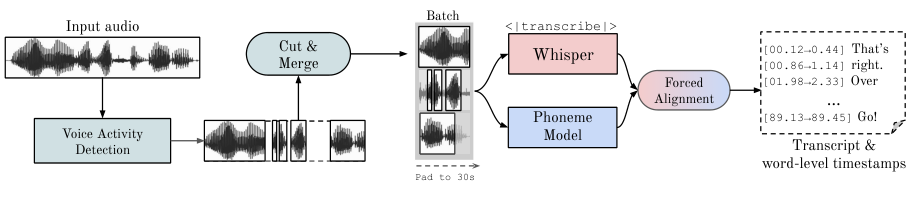
\includegraphics[width=\linewidth]{Images/Congnghelienquan/whisperx_pipeline.png}
    \caption[Pipeline nhận dạng và căn chỉnh thời gian từ của WhisperX]{Pipeline nhận dạng và căn chỉnh thời gian từ của WhisperX \parencite{ch3_whisperx}}
    \label{tech:fig:whisperx-pipeline}
\end{figure}

\subsubsection{Tổng hợp tiếng nói}

Text-to-Speech (TTS) chuyển văn bản thành tiếng nói. Các mô hình như VITS tiếp cận bài toán tổng hợp đầu cuối, kết hợp mô hình sinh và học đối kháng \parencite{ch3_vits}. Khi lựa chọn giải pháp tự triển khai hoặc dịch vụ TTS, cần cân nhắc độ rõ của giọng đọc, độ trễ, chi phí và khả năng lưu lại audio đã sinh.

Trong Wispace, TTS phục vụ phát câu hỏi và hướng dẫn trong luyện tập hoặc thi thử. Audio câu hỏi được chuẩn bị hoặc cache theo phiên bản nội dung và cấu hình giọng, giúp chuyển câu không phụ thuộc việc sinh tiếng nói tại thời điểm thi. TTS không tham gia đánh giá chất lượng câu trả lời của học viên.

\subsection{Các phương pháp đánh giá IELTS Speaking tự động}

IELTS Speaking sử dụng bốn tiêu chí: Fluency and Coherence, Lexical Resource, Grammatical Range and Accuracy và Pronunciation \parencite{ch3_ielts_scoring}. Hệ thống tự động cần kết hợp bằng chứng âm học và ngôn ngữ; một chỉ số như tốc độ nói hoặc độ chính xác transcript không thể đại diện đầy đủ cho cả bốn tiêu chí.

\subsubsection{Đánh giá phát âm}

Các phương pháp đánh giá phát âm có thể khai thác sự phù hợp giữa âm thanh và đơn vị ngôn ngữ, hoặc học quan hệ giữa biểu diễn âm thanh với điểm người chấm. HuBERT học biểu diễn tiếng nói thông qua dự đoán đơn vị ẩn; wav2vec 2.0 là một hướng học tự giám sát khác cho biểu diễn tiếng nói \parencite{ch3_wav2vec2}. Các encoder này cần được kết hợp với bộ dự đoán và dữ liệu nhãn phù hợp để phục vụ chấm điểm.

\begin{figure}[H]
    \centering
    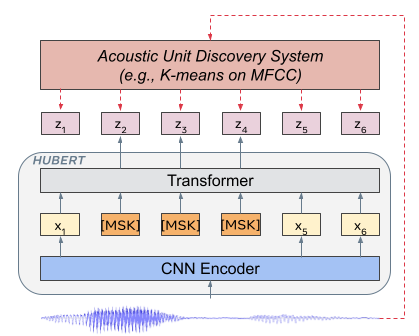
\includegraphics[width=.72\linewidth]{Images/Congnghelienquan/hubert_architecture.png}
    \caption[Cơ chế tiền huấn luyện HuBERT]{Cơ chế tiền huấn luyện HuBERT bằng dự đoán đơn vị ẩn tại các vị trí bị che \parencite{ch3_hubert}}
    \label{tech:fig:hubert-pretraining}
\end{figure}

Hình \ref{tech:fig:hubert-pretraining} minh họa cơ chế tiền huấn luyện HuBERT. Trong pipeline chấm Speaking, Wispace sử dụng HuBERT-base đóng băng tầng 9, tổng hợp đặc trưng, chuẩn hóa, giảm chiều bằng PCA và dự đoán bằng LightGBM cho nhánh Pronunciation của M5. Cách tiếp cận này giữ encoder cố định và huấn luyện bộ dự đoán phía sau. Điểm tổng từ biểu diễn audio không tự chứng minh khả năng xác định chính xác lỗi từng âm; phản hồi chi tiết cần có bằng chứng và phương pháp đánh giá tương ứng.

\subsubsection{Đánh giá độ trôi chảy}

Độ trôi chảy có thể được mô tả bằng tốc độ nói, tốc độ phát âm, độ dài chuỗi nói giữa các khoảng dừng và phân bố khoảng dừng. Cách tính cần thống nhất đơn vị, khoảng thời gian được xét và quy tắc loại trừ đoạn không có tiếng nói. Các dấu hiệu lặp hoặc tự sửa cũng có thể hỗ trợ phân tích, nhưng chịu ảnh hưởng của việc ASR giữ hay bỏ các hiện tượng này.

Nhánh M5 của Wispace kết hợp đặc trưng thời gian bằng luật cấu hình theo Part, cho phép giải thích đóng góp của từng chỉ số. Luật ban đầu cần được kiểm tra và hiệu chỉnh bằng dữ liệu người chấm. Fluency âm học không bao gồm toàn bộ Coherence; tốc độ nhanh hoặc ít khoảng dừng không đương nhiên tương ứng với điểm cao.

\subsubsection{Đánh giá ngôn ngữ}

Nhánh ngôn ngữ phân tích transcript trong ngữ cảnh câu hỏi để đánh giá phạm vi và cách dùng từ vựng, cấu trúc ngữ pháp và tổ chức ý. Các hướng tiếp cận gồm đặc trưng ngôn ngữ kết hợp mô hình dự đoán, mô hình ngôn ngữ được huấn luyện cho tác vụ và đánh giá theo rubric với đầu ra có cấu trúc. Việc lựa chọn cần xét khả năng dẫn chứng, tính ổn định và mức phù hợp với điểm người chấm.

M6 được thiết kế để đánh giá Lexical Resource, Grammatical Range and Accuracy và cung cấp bằng chứng Coherence. Nhận xét gắn với đoạn transcript và ngữ cảnh câu hỏi; metadata ASR giúp nhận biết vùng dữ liệu chưa chắc chắn. Một lỗi do ASR tạo ra không được mặc định quy thành lỗi của học viên, cũng không xem câu đã được ASR sửa là bằng chứng sử dụng ngôn ngữ chính xác.

\subsubsection{Tổng hợp và hiệu chuẩn điểm}

Tổng hợp kết quả kết hợp các nguồn bằng chứng; hiệu chuẩn điều chỉnh quan hệ giữa đầu ra mô hình với thang đánh giá mục tiêu. Hai bước này cần được phân biệt với việc chỉ làm tròn số. Dữ liệu hiệu chuẩn và đánh giá phải được tách phù hợp, đặc biệt theo người nói, để hạn chế kết quả quá lạc quan do cùng học viên xuất hiện ở nhiều tập.

M7 được thiết kế để tổng hợp đầu ra M5 và M6, hình thành bốn điểm tiêu chí, band tổng và phản hồi thống nhất. Fluency âm học được kết hợp với bằng chứng Coherence thay vì coi hai đại lượng là một. Công thức tổng hợp, quy tắc làm tròn và phiên bản hiệu chuẩn được quản lý rõ ràng. Đánh giá sử dụng sai số, tương quan và mức nhất quán với người chấm; không mặc định lấy trung bình điểm từng câu để xác định band toàn bài thi.

\subsection{Công nghệ lưu trữ và xử lý bất đồng bộ}

Hai hệ thống cần lưu dữ liệu nghiệp vụ, quản lý tệp và xử lý các tác vụ có thời gian thực thi khác nhau. Cơ sở dữ liệu, kho đối tượng, hàng đợi và cache đảm nhiệm các vai trò riêng, không thay thế lẫn nhau.

\subsubsection{Cơ sở dữ liệu quan hệ}

PostgreSQL và MySQL với InnoDB đều hỗ trợ giao dịch và các ràng buộc quan hệ, phù hợp với dữ liệu tài khoản, quyền truy cập và lịch sử xử lý \parencite{ch4_postgresql_transactions,ch3_mysql_innodb}. Việc lựa chọn cần dựa trên mô hình dữ liệu, thư viện tích hợp và yêu cầu vận hành, thay vì xếp hạng hiệu năng chung cho mọi loại truy vấn.

PostgreSQL được chọn cho Wispace và AIHub nhờ phù hợp với mô hình dữ liệu quan hệ và khả năng tích hợp .NET qua Npgsql. Dữ liệu nghiệp vụ có cấu trúc được lưu bằng bảng, khóa và ràng buộc; JSON có thể dùng cho một số đầu ra mô hình linh hoạt. Các dịch vụ Wispace sở hữu dữ liệu riêng, AIHub có database độc lập. Schema được quản lý bằng SQL migration của Flyway, còn EF Core đảm nhiệm ánh xạ và truy cập dữ liệu.

\subsubsection{Lưu trữ đối tượng}

Lưu trữ đối tượng tổ chức tệp theo khóa định danh, phù hợp với audio và tệp xuất có kích thước lớn. S3 hỗ trợ cấp quyền tải lên hoặc tải xuống có thời hạn qua presigned URL \parencite{ch3_s3_presigned}. So với lưu nội dung tệp trực tiếp trong bảng nghiệp vụ, cách tổ chức này cho phép tách đường truyền tệp và chính sách lưu trữ khỏi truy vấn quan hệ.

Wispace lưu audio trên S3; PostgreSQL giữ object key, kích thước, checksum và trạng thái xác minh. AIHub sử dụng kho đối tượng cho tệp xuất dữ liệu học thuật. Backend kiểm tra quyền trước khi cấp URL; URL tạm không thay thế bước kiểm tra tệp và xác nhận bài nộp.

\subsubsection{Hàng đợi thông điệp}

Hàng đợi giúp tách thời điểm tiếp nhận yêu cầu khỏi thời điểm xử lý. RabbitMQ hỗ trợ publisher confirm và consumer acknowledgement cho các giai đoạn giao nhận thông điệp \parencite{ch4_rabbitmq_confirms}; prefetch giới hạn số thông điệp chưa xác nhận được giao cho consumer. Kafka tổ chức sự kiện theo topic và partition, hỗ trợ retention và đọc lại bằng offset \parencite{ch4_kafka_intro}.

\begin{table}[H]
\centering
\caption{Đối chiếu RabbitMQ và Kafka theo nhu cầu của đề tài}
\label{tech:tab:broker-comparison}
\small
\renewcommand{\arraystretch}{1.2}
\begin{tabularx}{\linewidth}{|>{\raggedright\arraybackslash}X|>{\raggedright\arraybackslash}X|>{\raggedright\arraybackslash}X|}
\hline
\textbf{Tiêu chí} & \textbf{RabbitMQ trong thiết kế} & \textbf{Kafka khi áp dụng} \\ \hline
Phân phối công việc & Queue cho nhóm worker, xác nhận từng thông điệp. & Cần phối hợp trạng thái job với cách tiêu thụ topic và quản lý offset. \\ \hline
Khai thác lịch sử & Queue phục vụ vận chuyển; dữ liệu gốc do database quản lý. & Retention và offset hỗ trợ nhiều nhóm đọc lại luồng sự kiện. \\ \hline
Công việc kéo dài & Kết hợp prefetch và giới hạn đồng thời của worker. & Cần thiết kế tiến độ xử lý, phân vùng và phân công lại consumer phù hợp. \\ \hline
Nhu cầu đề tài & Chấm Speaking, tác vụ AI dài và xuất dữ liệu nền. & Cân nhắc khi cần nền tảng phân tích luồng hoặc đọc lại lượng lớn sự kiện. \\ \hline
\end{tabularx}
\end{table}

RabbitMQ được chọn vì thiết kế ưu tiên điều phối công việc chấm và tác vụ nền. Lựa chọn này không khẳng định RabbitMQ luôn nhanh hơn hoặc Kafka không thể xử lý tác vụ. Thông điệp chỉ chứa định danh và tham chiếu; audio nằm trong S3. Trạng thái job, outbox và cơ chế chống trùng được lưu bền vững để hỗ trợ xử lý lại; broker không tự bảo đảm một tác vụ chỉ chạy đúng một lần.

\subsubsection{Bộ nhớ đệm}

Redis cung cấp các cấu trúc dữ liệu trong bộ nhớ để lưu dữ liệu cần truy cập nhanh \parencite{ch4_redis}. Cache giúp giảm truy vấn lặp đối với nội dung và cấu hình ít thay đổi; thời hạn và cơ chế cập nhật cache cần phù hợp với nguồn dữ liệu. Redis cũng có thể hỗ trợ bộ đếm giới hạn tốc độ truy cập.

Wispace dùng Redis cho nội dung đề và cấu hình thường đọc; AIHub dùng cho cấu hình dịch vụ và giới hạn tốc độ theo tổ chức hoặc khóa API. Điểm số, bài nộp và sổ hạn mức có thẩm quyền vẫn do PostgreSQL quản lý. Rate limit kiểm soát tần suất gửi yêu cầu, còn quota là quyền sử dụng nghiệp vụ; hai cơ chế cần được phân biệt.

\subsection{Công nghệ cung cấp và quản lý dịch vụ AI}

Cung cấp AI qua API cần kết hợp thực thi mô hình với quản lý hợp đồng dữ liệu, phiên bản, quyền truy cập và lịch sử sử dụng. Đây là cơ sở cho đường gọi nội bộ của Wispace và dịch vụ B2B của AIHub.

\subsubsection{Cung cấp mô hình qua API}

OpenAPI mô tả đường dẫn, dữ liệu yêu cầu, phản hồi và cơ chế bảo mật của HTTP API \parencite{ch3_openapi}. Hợp đồng rõ ràng giúp backend nghiệp vụ và dịch vụ Python phát triển độc lập, đồng thời hỗ trợ kiểm thử tương thích khi thay đổi cấu trúc dữ liệu.

Tác vụ ngắn có thể trả kết quả đồng bộ; tác vụ dài trả mã công việc để bên gọi theo dõi trạng thái. Wispace Assessment gọi lớp điều phối chấm Speaking bằng FastAPI, nơi M5, M6 và M7 được phối hợp theo hợp đồng đánh giá. AIHub kiểm tra yêu cầu B2B trước khi chuyển đến dịch vụ mô hình. Cả hai cần trạng thái lỗi rõ ràng và mã chống trùng cho các thao tác có thể được gửi lại.

\subsubsection{Quản lý phiên bản và định tuyến mô hình}

Một phiên bản mô hình gồm không chỉ trọng số mà còn cấu hình tiền xử lý, tokenizer, schema đầu ra và các quy tắc hậu xử lý liên quan. Thay đổi một thành phần có thể làm kết quả khác nhau; vì vậy mỗi phản hồi cần truy vết được cấu hình thực thi tương ứng.

Wispace gắn kết quả với phiên bản pipeline và hiệu chuẩn. AIHub sử dụng model route để ánh xạ dịch vụ với mô hình hoặc nhà cung cấp được cấu hình. Phương án dự phòng chỉ được dùng khi tương thích với chức năng và hợp đồng dữ liệu; mô hình sinh nội dung không mặc định thay thế Scoring Model. Khi thay phiên bản, cần kiểm tra dữ liệu, chất lượng và khả năng tương thích trước khi chuyển lưu lượng.

\subsubsection{Quản lý truy cập và sử dụng API}

Quản lý API kết hợp xác thực bên gọi, phân quyền dịch vụ, giới hạn tốc độ và kiểm soát hạn mức. Khóa API nhận diện một ứng dụng hoặc đối tác, nhưng quyền truy cập vẫn cần được kiểm tra theo tổ chức, dịch vụ và trạng thái credentials. Bí mật được sử dụng từ máy chủ đối tác, không đưa vào frontend công khai.

AIHub quản lý tổ chức B2B, khóa API, gói dịch vụ và usage. Wispace quản lý quyền học viên và hạn mức luyện tập hoặc thi thử tại lớp nghiệp vụ riêng. Với tác vụ dài, hạn mức được giữ, chốt hoặc giải phóng theo trạng thái xử lý; yêu cầu gửi lại phải được nhận diện để tránh tính lặp. Usage ghi định danh yêu cầu, phiên bản mô hình, thời gian xử lý và đơn vị tiêu thụ phục vụ theo dõi, đối soát.

\subsubsection{Quản lý dữ liệu học thuật}

Dữ liệu học thuật cần lưu nguồn, phiên bản và quyết định thẩm định, tách đầu ra AI ban đầu khỏi bản chỉnh sửa. Dữ liệu SFT gồm đầu vào và đầu ra mục tiêu; dữ liệu DPO gồm các phương án được chọn và bị từ chối cho cùng đầu vào. DPO tối ưu theo dữ liệu ưu tiên tương đối thay vì chỉ học một đầu ra mục tiêu \parencite{ch3_dpo}.

Academic Lab của AIHub tổ chức quá trình sinh mẫu, hiệu đính, thẩm định và xuất bộ dữ liệu có phiên bản. Chỉ mẫu đáp ứng điều kiện mới được đưa vào bản xuất; cần kiểm tra quyền sử dụng, thông tin cá nhân và trùng lặp giữa các tập. Dữ liệu Writing SFT/DPO phục vụ tác vụ tương ứng, không mặc định trở thành nhãn chấm Speaking. Với Wispace, dữ liệu audio và điểm người chấm được quản lý theo sự đồng ý của học viên và mục đích huấn luyện, hiệu chuẩn, đánh giá.

%=========================
% CHƯƠNG 4 - CÔNG NGHỆ SỬ DỤNG
% Tệp được nạp sau chương Công nghệ liên quan trong main.tex.
%=========================

\section{Công nghệ sử dụng}
\label{sec:technologies}

Chương này trình bày các công nghệ được lựa chọn cho Wispace Speaking và AIHub. Wispace phục vụ luyện tập, thi thử và đánh giá IELTS Speaking; AIHub cung cấp dịch vụ AI qua API cho đối tác B2B và công cụ học thuật nội bộ. Hai hệ thống có frontend, backend và dữ liệu độc lập, cùng sử dụng React, ASP.NET Core, PostgreSQL và các dịch vụ AI bằng Python FastAPI. Nội dung tập trung vào vai trò và cơ sở lựa chọn công nghệ; cách tổ chức thành phần và luồng tích hợp được trình bày ở Chương 7.

\subsection{Tiêu chí lựa chọn công nghệ}

Việc lựa chọn công nghệ dựa trên bốn tiêu chí:
\begin{itemize}
    \item \textbf{Phù hợp nghiệp vụ:} hỗ trợ ghi âm, quản lý phiên thi, chấm Speaking và theo dõi tiến bộ của Wispace; quản lý tổ chức, khóa API, hạn mức và dữ liệu học thuật của AIHub.
    \item \textbf{Phân tách loại tải:} tách xử lý HTTP và dữ liệu nghiệp vụ khỏi các tác vụ AI có thời gian thực thi dài, cho phép điều chỉnh tài nguyên API và suy luận riêng.
    \item \textbf{Bảo vệ dữ liệu:} hỗ trợ giao dịch, kiểm soát truy cập và truy vết thay đổi đối với bài làm, điểm số, hạn mức và dữ liệu từng tổ chức.
    \item \textbf{Khả năng tích hợp và vận hành:} có tài liệu rõ ràng, hệ sinh thái phù hợp, hỗ trợ kiểm thử và triển khai nhất quán giữa môi trường phát triển và máy chủ.
\end{itemize}

\subsection{Tổng hợp công nghệ}

Bảng \ref{tech:tab:stack} tổng hợp các thành phần chính của thiết kế. Phiên bản cụ thể được cố định trong cấu hình dự án và môi trường triển khai, bảo đảm tương thích giữa runtime, thư viện truy cập dữ liệu và mô hình AI.

\begingroup
\small\setstretch{1.1}
\renewcommand{\arraystretch}{1.2}
\begin{longtable}{|>{\raggedright\arraybackslash}p{\dimexpr.20\linewidth-2\tabcolsep-2\arrayrulewidth\relax}|>{\raggedright\arraybackslash}p{\dimexpr.27\linewidth-2\tabcolsep-\arrayrulewidth\relax}|>{\raggedright\arraybackslash}p{\dimexpr.53\linewidth-2\tabcolsep-\arrayrulewidth\relax}|}
\caption{Công nghệ sử dụng cho Wispace và AIHub}\label{tech:tab:stack}\\\hline
\textbf{Nhóm} & \textbf{Công nghệ} & \textbf{Vai trò} \\ \hline
\endfirsthead
\hline
\textbf{Nhóm} & \textbf{Công nghệ} & \textbf{Vai trò} \\ \hline
\endhead
Giao diện & React & Giao diện học viên, quản trị Wispace; Portal B2B và Academic Lab của AIHub. \\ \hline
Ghi âm web & MediaRecorder & Thu âm câu trả lời Speaking trên trình duyệt và cung cấp dữ liệu để tải lên. \\ \hline
Backend & C\#, ASP.NET Core & API, xác thực, phân quyền và xử lý nghiệp vụ của từng hệ thống. \\ \hline
Truy cập dữ liệu & EF Core, Npgsql & Ánh xạ entity, theo dõi thay đổi và truy vấn PostgreSQL. \\ \hline
Migration & Flyway & Quản lý phiên bản cấu trúc database bằng các lệnh SQL viết thủ công. \\ \hline
Dịch vụ AI & Python, FastAPI & Cung cấp API suy luận và kiểm tra hợp đồng dữ liệu đầu vào, đầu ra. \\ \hline
Mô hình & Scoring Model; mô hình sinh nội dung qua adapter & Chấm Speaking bằng mô hình tự huấn luyện; cung cấp tác vụ AI và sinh mẫu học thuật theo cấu hình. \\ \hline
Cơ sở dữ liệu & PostgreSQL & Lưu dữ liệu nghiệp vụ, trạng thái xử lý, điểm số và lịch sử sử dụng. \\ \hline
Lưu trữ tệp & S3 & Lưu audio riêng tư của Wispace; kho đối tượng phục vụ tệp xuất nội bộ của AIHub. \\ \hline
Bất đồng bộ & RabbitMQ,.NET Worker & Phân phối công việc nền, tiếp nhận sự kiện và điều phối xử lý. \\ \hline
Bộ nhớ đệm & Redis & Cache nội dung, cấu hình và hỗ trợ giới hạn tốc độ truy cập. \\ \hline
Triển khai & Docker, Docker Compose & Đóng gói dịch vụ; tổ chức môi trường phát triển và kiểm thử tích hợp. \\ \hline
Phát triển & Git, GitHub; OpenAPI & Quản lý phiên bản mã nguồn và mô tả hợp đồng API. \\ \hline
\end{longtable}
\endgroup

\subsection{Giao diện web và ghi âm}
\subsubsection{React}

React tổ chức giao diện thành các component, hỗ trợ cập nhật màn hình theo trạng thái và tái sử dụng thành phần. Cách tổ chức này phù hợp với các màn hình có nhiều trạng thái như đang ghi âm, đang tải audio, chờ chấm và hiển thị kết quả.

Wispace sử dụng React cho kho đề, luyện tập, thi thử, lịch sử kết quả và quản trị. AIHub sử dụng một ứng dụng React riêng cho quản lý tổ chức, khóa API, theo dõi usage và thẩm định mẫu học thuật. Hai frontend gọi backend tương ứng, không dùng chung phiên đăng nhập hoặc suy ra quyền truy cập của nhau.

\subsubsection{Ghi âm trên trình duyệt}

MediaRecorder cung cấp khả năng ghi dữ liệu từ luồng media của trình duyệt \parencite{ch4_mediarecorder}. Trong Wispace, giao diện xin quyền micro, ghi câu trả lời và theo dõi trạng thái tải lên. Ứng dụng kiểm tra định dạng mà trình duyệt hỗ trợ; dịch vụ AI chuẩn hóa audio về định dạng đầu vào của Scoring Model.

Audio được tải trực tiếp lên S3 bằng quyền truy cập có thời hạn do backend cấp. Trình duyệt không giữ khóa truy cập kho lưu trữ. Trạng thái hoàn tất bài nộp và thời hạn phiên thi được backend xác nhận, thay vì chỉ dựa vào bộ đếm hoặc thông báo thành công trên giao diện.

\subsection{Backend và truy cập dữ liệu}
\subsubsection{ASP.NET Core}

ASP.NET Core là nền tảng xây dựng ứng dụng web đa nền tảng trong hệ sinh thái.NET, có các cơ chế phục vụ API, dependency injection và middleware. C\# hỗ trợ tổ chức mô hình miền, hợp đồng dữ liệu và các lớp xử lý nghiệp vụ theo kiểu dữ liệu rõ ràng.

Wispace tổ chức backend thành các dịch vụ Core, Learning \& Exam, Assessment và Progress \& Reporting. Việc tách dịch vụ cho phép mở rộng luồng tiếp nhận bài làm và chấm điểm theo nhu cầu riêng. AIHub sử dụng backend ASP.NET Core độc lập theo modular monolith, phân chia các module Access, Gateway, Catalog, Usage và Academic Lab. Cách tổ chức này giữ nghiệp vụ quản lý B2B thống nhất trong khi dịch vụ suy luận vẫn có thể triển khai riêng.

Xác thực người dùng được kết hợp với phân quyền tại API và đối tượng dữ liệu. Đối với AIHub, thông tin xác thực của đối tác phải gắn với tổ chức, dịch vụ được cấp quyền và hạn mức sử dụng. Khóa bí mật B2B được dùng tại máy chủ của đối tác, không nhúng trong ứng dụng React.

\subsubsection{Entity Framework Core và Npgsql}

Entity Framework Core ánh xạ các entity C\# với bảng và hỗ trợ truy vấn, cập nhật dữ liệu; DbContext theo dõi thay đổi của các entity được quản lý. Npgsql cung cấp tích hợp EF Core với PostgreSQL \parencite{ch7_npgsql}. Cấu hình ánh xạ mô tả cấu trúc bảng đã được quản lý bằng migration, không tự tạo bảng khi ứng dụng khởi động.

Giao dịch dữ liệu được giới hạn trong database sở hữu nghiệp vụ. Những thay đổi liên quan nhiều dịch vụ được phối hợp bằng API và sự kiện. Cách sử dụng này tránh giữ giao dịch cơ sở dữ liệu trong suốt thời gian tải audio hoặc gọi mô hình AI.

\subsubsection{Flyway và SQL migration}

Flyway quản lý thứ tự và lịch sử thay đổi cấu trúc database bằng các file SQL có phiên bản \parencite{ch4_flyway}. Các lệnh tạo bảng, khóa, ràng buộc và chỉ mục được viết thủ công, chẳng hạn trong file \texttt{V1\_\_create\_users.sql}. Flyway chạy qua CLI hoặc container ở bước triển khai, độc lập với backend.NET. EF Core phụ trách ánh xạ và truy cập dữ liệu, không quản lý migration hoặc tự sinh bảng. Sau mỗi thay đổi schema, cấu hình ánh xạ được cập nhật để khớp với database.

Mỗi dịch vụ Wispace có bộ SQL migration và lịch sử Flyway riêng; AIHub có bộ migration độc lập. Migration được chạy ở bước triển khai có kiểm soát, trước khi phiên bản ứng dụng tương ứng phục vụ yêu cầu. Các bản sao API không tự chạy migration khi khởi động. File migration đã áp dụng được giữ nguyên; thay đổi tiếp theo được bổ sung bằng một phiên bản mới.

\subsection{Dịch vụ AI và mô hình}
\subsubsection{Python FastAPI}

FastAPI hỗ trợ xây dựng API Python với khai báo kiểu dữ liệu, kiểm tra dữ liệu bằng Pydantic và mô tả API theo OpenAPI. Python phù hợp để tích hợp mã tiền xử lý và suy luận của mô hình, trong khi.NET tiếp tục quản lý nghiệp vụ, quyền truy cập và dữ liệu bền vững.

Trong Wispace, Assessment Worker gọi trực tiếp FastAPI để xử lý audio và thực thi Scoring Model. Đầu ra được kiểm tra trước khi lưu điểm và nhận xét. Đối với AIHub, backend định tuyến yêu cầu đến dịch vụ mô hình hoặc nhà cung cấp theo adapter và cấu hình. Hai đường tích hợp này độc lập: Wispace không phải đi qua API B2B của AIHub để chấm Speaking.

Các tác vụ suy luận dài được điều phối bằng worker và hàng đợi. Khả năng lập trình bất đồng bộ của API không thay thế việc giới hạn số lượt suy luận, quản lý tài nguyên GPU và kiểm soát thời gian xử lý.

\subsubsection{Scoring Model và mô hình sinh nội dung}

Scoring Model của Wispace được thiết kế theo pipeline M5--M6--M7. M5 Acoustic phân tích audio và ước lượng Pronunciation, Fluency; M6 Linguistic đánh giá Lexical Resource, Grammatical Range and Accuracy cùng bằng chứng Coherence từ transcript và ngữ cảnh câu hỏi. M7 Fusion tổng hợp và hiệu chuẩn các nhánh để trả bốn điểm tiêu chí, band tổng và nhận xét thống nhất. Mỗi kết quả gắn với phiên bản mô hình, rubric và metadata chất lượng; transcript chưa xác minh được xử lý theo mức độ tin cậy của dữ liệu. Chất lượng chấm và cơ chế hiệu chuẩn được đánh giá bằng dữ liệu người chấm.

AIHub quản lý danh mục dịch vụ, model route và thông tin sử dụng. Academic Lab sử dụng mô hình sinh nội dung để tạo mẫu, sau đó chuyên viên hiệu đính và thẩm định trước khi xuất dữ liệu. Bản gốc, phiên bản chỉnh sửa và quyết định review được lưu để truy vết. Dữ liệu Writing phục vụ SFT/DPO được tách khỏi dữ liệu đánh giá Speaking, không mặc định được dùng làm nhãn chuẩn cho Scoring Model.

\subsection{Cơ sở dữ liệu và lưu trữ}
\subsubsection{PostgreSQL}

PostgreSQL được lựa chọn làm cơ sở dữ liệu quan hệ cho cả hai hệ thống. Cơ chế giao dịch hỗ trợ cập nhật một nhóm thay đổi theo tính chất toàn bộ hoặc không thay đổi. Đây là cơ sở để thiết kế các thao tác cần tính nhất quán như giữ hạn mức, chốt kết quả và ghi nhận thanh toán.

Wispace phân tách dữ liệu theo dịch vụ: tài khoản và kho đề tại Core; phiên học và metadata audio tại Learning; job và kết quả tại Assessment; dữ liệu tổng hợp tại Reporting. AIHub có database riêng cho tổ chức, credentials, dịch vụ, usage và mẫu học thuật. Liên kết xuyên dịch vụ Wispace là tham chiếu logic, không tạo khóa ngoại giữa các database.

Dữ liệu có cấu trúc được tổ chức bằng bảng và ràng buộc quan hệ. Kiểu \texttt{jsonb} hỗ trợ lưu một số cấu trúc linh hoạt như đầu ra mô hình hoặc metadata \parencite{ch4_postgresql_json}. Các thuộc tính cần tra cứu, đối soát hoặc kiểm soát tính duy nhất vẫn được thiết kế thành cột rõ ràng.

\subsubsection{S3}

S3 được dùng để lưu audio, tách nội dung tệp khỏi cơ sở dữ liệu và đường truyền API nghiệp vụ. PostgreSQL lưu object key, kích thước, checksum và trạng thái xác minh. Thiết kế này giúp backend quản lý quyền và metadata trong khi việc truyền tệp diễn ra trực tiếp với kho lưu trữ.

Audio cá nhân nằm trong vùng lưu trữ riêng tư, được truy cập bằng URL có thời hạn. Việc xóa bản ghi, kiểm tra tệp tải lên và sử dụng audio cho huấn luyện tuân theo quyền sở hữu và chính sách dữ liệu của Wispace. Tệp xuất nội bộ của AIHub được quản lý riêng theo quyền của Academic Lab.

\subsubsection{Redis}

Redis cung cấp cấu trúc dữ liệu trong bộ nhớ, được sử dụng cho các dữ liệu cần truy cập nhanh. Wispace dùng cache cho nội dung đề và cấu hình thường đọc; AIHub dùng cache cấu hình dịch vụ và hỗ trợ giới hạn tốc độ theo tổ chức hoặc khóa API.

Dữ liệu cache có thời hạn và cơ chế cập nhật khi nguồn thay đổi. Điểm số, sổ hạn mức và trạng thái nghiệp vụ có thẩm quyền vẫn được lưu trong PostgreSQL, tránh phụ thuộc vào dữ liệu tạm khi Redis khởi động lại hoặc cache hết hạn.

\subsection{Hàng đợi và xử lý nền}
\subsubsection{RabbitMQ và .NET Worker}

RabbitMQ được lựa chọn để chuyển công việc nền và sự kiện giữa các thành phần. Publisher confirm xác nhận broker tiếp nhận thông điệp; consumer acknowledgement xác nhận phía nhận đã xử lý thông điệp theo quy ước của ứng dụng..NET Worker tiếp nhận công việc, gọi dịch vụ cần thiết và cập nhật trạng thái xử lý.

Wispace sử dụng hàng đợi để tách việc nộp bài khỏi thời gian suy luận và phân phối công việc đến các worker chấm. AIHub sử dụng xử lý nền cho tác vụ AI dài và xuất dữ liệu. Các nhóm công việc và sự kiện có hàng đợi riêng; audio và tệp xuất được lưu trong kho đối tượng, thông điệp chỉ mang định danh và tham chiếu cần thiết.

Outbox lưu thông điệp chờ phát cùng giao dịch nghiệp vụ; consumer sử dụng định danh thông điệp để chống xử lý trùng. Lỗi tạm thời được thử lại có giới hạn, còn lỗi kết thúc được ghi nhận để đối soát. Chi tiết trạng thái và luồng xử lý được trình bày ở Chương 7.

\subsubsection{Cơ sở lựa chọn RabbitMQ thay vì Kafka}

Luồng chấm Speaking cần phân phối các công việc độc lập, có thời gian xử lý không đồng đều, đến nhóm worker có năng lực giới hạn. Thiết kế lựa chọn RabbitMQ để tập trung vào quản lý hàng đợi, xác nhận xử lý và điều phối công việc. Số người dùng đồng thời không trực tiếp quyết định lựa chọn broker; cần xem xét số bài nộp, thời gian chấm và độ trễ hàng đợi.

Kafka cung cấp mô hình lưu luồng sự kiện theo topic, hỗ trợ retention và đọc lại dữ liệu bằng offset. Mô hình này phù hợp khi nhiều nhóm xử lý cần khai thác cùng lịch sử sự kiện hoặc thực hiện phân tích luồng. Phạm vi hiện tại của Wispace và AIHub ưu tiên điều phối tác vụ và thông báo thay đổi nghiệp vụ; dữ liệu gốc được quản lý trong PostgreSQL. Vì vậy, RabbitMQ được chọn cho thiết kế này; Kafka có thể được đánh giá khi phát sinh nhu cầu khai thác lịch sử sự kiện ở quy mô lớn.

\subsection{Đóng gói, phát triển và kiểm thử}

Docker đóng gói backend.NET, dịch vụ Python và các thành phần hạ tầng trong môi trường chạy được cấu hình rõ ràng. Docker Compose mô tả và khởi chạy ứng dụng nhiều container bằng một cấu hình thống nhất \parencite{ch4_docker_compose}; trong đề tài, công cụ này phục vụ phát triển và kiểm thử tích hợp.

Git và GitHub quản lý phiên bản mã nguồn, thay đổi cấu hình và phối hợp phát triển. Dependency được cố định theo từng ứng dụng; cấu hình kết nối và bí mật được cấp qua môi trường triển khai. Mã nguồn và cấu hình công khai không chứa khóa API, mật khẩu database hoặc khóa truy cập S3.

OpenAPI mô tả hợp đồng API của backend và FastAPI, phục vụ tích hợp và kiểm thử. Các kiểm tra tập trung vào phân quyền, bài nộp trùng, xử lý lại thông điệp, hạn mức và lỗi suy luận. Đánh giá tải cần đo riêng độ trễ API, tốc độ tải audio, độ dài hàng đợi và thời gian chấm; việc đóng gói thành công không thay thế kiểm thử các chỉ tiêu này.

% Sections/05-KhaiThacYeuCau.tex
\section{Khai thác yêu cầu}

Chương này xác định tác nhân, yêu cầu chức năng, phi chức năng và dữ liệu của hai hệ thống Wispace Speaking và AIHub. Wispace phục vụ luyện tập, thi thử và đánh giá kỹ năng Nói IELTS; AIHub cung cấp API mô hình cho đối tác B2B và công cụ quản lý chất lượng mô hình nội bộ. Các yêu cầu làm cơ sở cho phân tích nghiệp vụ ở Chương 6 và thiết kế ở Chương 7.

\subsection{Hệ thống AI hỗ trợ chấm điểm và cá nhân hóa luyện tập kỹ năng Nói IELTS}
\label{subsec:wispace_system_spec}

\subsubsection{Mô tả tổng quan về hệ thống}
Wispace Speaking hỗ trợ luyện tập theo Part và thi thử IELTS với kho đề Cambridge 1--20, Forecast hoặc đề tự thêm. Scoring Model do Wispace tự huấn luyện nhận audio, trả transcript, lỗi phát âm và band theo bốn tiêu chí Fluency \& Coherence, Lexical Resource, Grammatical Range \& Accuracy và Pronunciation. Kết quả được dùng để theo dõi tiến bộ và xây dựng lộ trình cá nhân hóa.

Thi thử mô phỏng buổi thi 11--14 phút, có giọng đọc câu hỏi và không cho nghe lại hoặc ghi lại. Tài khoản, gói Self-practice và thanh toán PayOS được dùng chung trong nền tảng Wispace Writing/Speaking. Dữ liệu dùng để cải thiện mô hình cần sự đồng ý của học viên và nhãn đánh giá của chuyên gia.

\subsubsection{Các nhóm người dùng và chức năng}
\begin{itemize}
\item \textbf{Khách:} xem kho đề, đăng ký, đăng nhập và khôi phục mật khẩu.
\item \textbf{Học viên:} luyện tập, thi thử, xem kết quả, quản lý hồ sơ và mua gói dịch vụ.
\item \textbf{Kiểm duyệt viên:} quản lý kho đề, duyệt đề cộng đồng và xử lý báo cáo nội dung.
\item \textbf{Quản trị viên:} quản lý người dùng, gói, hạn mức và thống kê vận hành.
\end{itemize}
Hệ thống tích hợp Scoring Model, TTS, Google OAuth, email, PayOS và Tracking-System. PostgreSQL và S3 lưu dữ liệu nghiệp vụ và audio.

\subsubsection{Yêu cầu chức năng}
Các yêu cầu chức năng của hệ thống được phân rã chi tiết theo từng nhóm người dùng thông qua các bảng dưới đây.

\begin{table}[H]
\centering
\caption{Yêu cầu chức năng của Khách (chưa đăng nhập)}
\label{wispace:tab:func_guest}
\small
\begin{tabular}{|p{4.2cm}|p{\dimexpr\linewidth-4.2cm-4\tabcolsep-3\arrayrulewidth\relax}|}
\hline
\textbf{Chức năng} & \textbf{Mô tả} \\
\hline
Đăng ký tài khoản & Khách nhập email, mật khẩu. Hệ thống gửi mã OTP 6 chữ số qua email để kích hoạt tài khoản, sau đó cấp gói dùng thử và chuyển người dùng sang bước onboarding. \\
\hline
Đăng nhập & Đăng nhập bằng email và mật khẩu hoặc bằng tài khoản Google. Sau khi xác thực thành công, hệ thống chuyển người dùng đến trang tương ứng với vai trò của họ. \\
\hline
Quên mật khẩu & Khách nhập email đã đăng ký, nhận mã OTP qua email, xác thực OTP rồi đặt mật khẩu mới. \\
\hline
Xem danh sách đề & Xem danh sách đề thi Cambridge và Forecast (chỉ hiển thị tiêu đề và chủ đề). Khi bấm luyện tập, hệ thống yêu cầu đăng nhập. \\
\hline
\end{tabular}
\end{table}

\begin{table}[H]
\centering
\caption{Yêu cầu chức năng của Học viên}
\label{wispace:tab:func_student}
\small
\begin{tabular}{|p{4.2cm}|p{\dimexpr\linewidth-4.2cm-4\tabcolsep-3\arrayrulewidth\relax}|}
\hline
\textbf{Chức năng} & \textbf{Mô tả} \\
\hline
Đăng xuất & Đăng xuất khỏi thiết bị hiện tại hoặc tất cả thiết bị. Nếu đang làm bài thi thử, hệ thống hỏi người dùng có muốn nộp phần đã làm hay không. Hệ thống vô hiệu hoá token và đưa người dùng về trang đăng nhập. \\
\hline
Quản lý hồ sơ cá nhân & Cập nhật tên, ảnh đại diện, band mục tiêu, ngày thi dự kiến và giọng giám khảo ưa thích. Kiểm tra micro, xem gói đang dùng và hạn mức còn lại, đổi mật khẩu, xoá file ghi âm hoặc xoá tài khoản. \\
\hline
Xem và tìm kiếm đề thi & Duyệt đề theo các nguồn: Cambridge 1--20, Forecast theo quý, Đề của tôi và Cộng đồng. Lọc theo Part, chủ đề và trạng thái đã làm. Từ trang chi tiết đề, người dùng chọn Luyện tập hoặc Thi thử. \\
\hline
Thêm đề thi & Tự tạo đề cho Part 1, Part 2 (cue card), Part 3 hoặc cả bộ đề. Hệ thống kiểm tra tính hợp lệ và phát hiện trùng lặp, lưu đề ở chế độ riêng tư; người dùng có thể đề xuất công khai để Moderator duyệt. \\
\hline
Luyện tập theo Part & Chọn câu hỏi, nghe giọng đọc (TTS) của giám khảo, ghi âm câu trả lời, nghe lại hoặc ghi âm lại trước khi nộp. Với Part 2 có 60 giây chuẩn bị kèm giấy nháp và thời gian nói tối đa 2 phút. Audio được gửi cho Scoring Model chấm và trả kết quả từng câu. \\
\hline
Xem kết quả và luyện lại & Xem band tổng và 4 tiêu chí (FC, LR, GRA, P), transcript có tô lỗi, chỉ số độ trôi chảy và câu trả lời mẫu. Bấm vào từ phát âm sai để nghe lại và so sánh với phát âm chuẩn. Có thể luyện lại và so sánh kết quả giữa lần trước và lần này. \\
\hline
Thi thử như thật & Chọn bộ đề đầy đủ và kiểm tra thiết bị. Giám khảo AI hỏi bằng giọng nói lần lượt Part 1, Part 2, Part 3. Không cho nghe lại, ghi âm lại hay tạm dừng. Khi kết thúc, hệ thống chấm bài ở chế độ nền và thông báo khi báo cáo sẵn sàng. \\
\hline
Xem lịch sử và tiến bộ & Xem danh sách các bài đã làm, lọc theo Part, nguồn đề và ngày làm. Theo dõi biểu đồ band theo thời gian và danh sách các lỗi lặp lại nhiều nhất. \\
\hline
Mua gói dịch vụ & Chọn gói Self-practice (1, 3, 6 hoặc 12 tháng), dùng chung cho Writing và Speaking. Hệ thống tạo liên kết thanh toán PayOS; sau khi PayOS xác nhận, quyền lợi trả phí được kích hoạt cho cả Writing và Speaking. \\
\hline
\end{tabular}
\end{table}

\begin{table}[H]
\centering
\caption{Yêu cầu chức năng của Moderator}
\label{wispace:tab:func_moderator}
\small
\begin{tabular}{|p{4.2cm}|p{\dimexpr\linewidth-4.2cm-4\tabcolsep-3\arrayrulewidth\relax}|}
\hline
\textbf{Chức năng} & \textbf{Mô tả} \\
\hline
Quản lý kho đề Cambridge/Forecast & Thêm, sửa, ẩn đề theo cấu trúc Quyển $\rightarrow$ Test $\rightarrow$ Part $\rightarrow$ Câu hỏi. Nhập hàng loạt bằng file CSV/JSON và nhận báo cáo các dòng lỗi. Tạo bộ Forecast theo quý và sinh audio cho câu hỏi. \\
\hline
Duyệt đề cộng đồng & Xem hàng chờ duyệt, sau đó duyệt, từ chối kèm lý do hoặc gộp với đề trùng. Hệ thống thông báo kết quả cho tác giả. \\
\hline
Xử lý báo cáo đề & Xem các báo cáo đề sai, trùng hoặc vi phạm. Moderator quyết định gỡ đề, sửa đề hoặc bỏ qua báo cáo. \\
\hline
\end{tabular}
\end{table}

\begin{table}[H]
\centering
\caption{Yêu cầu chức năng của Quản trị viên hệ thống}
\label{wispace:tab:func_admin}
\small
\begin{tabular}{|p{4.2cm}|p{\dimexpr\linewidth-4.2cm-4\tabcolsep-3\arrayrulewidth\relax}|}
\hline
\textbf{Chức năng} & \textbf{Mô tả} \\
\hline
Tìm kiếm người dùng & Tìm theo email hoặc tên; lọc theo vai trò, gói dịch vụ, trạng thái và ngày đăng ký. Xem trang chi tiết của từng người dùng. \\
\hline
Cập nhật trạng thái người dùng & Khoá hoặc mở khoá tài khoản, đổi vai trò, cộng thêm quota thủ công. Bắt buộc nhập lý do; thay đổi được áp dụng ngay, ghi nhật ký và gửi email thông báo cho người dùng. \\
\hline
Quản lý gói và quota & Cấu hình gói dùng chung, giá và hạn mức từng tính năng cho Writing và Speaking: số bài viết được chấm, số câu nói được chấm và số lượt thi thử mỗi ngày. \\
\hline
Xem thống kê & Xem doanh thu, số người dùng hoạt động, số bài Speaking đã chấm và chi phí AI/STT theo ngày. \\
\hline
\end{tabular}
\end{table}
\newpage

\subsubsection{Yêu cầu phi chức năng}
Các yêu cầu dưới đây xác định chất lượng phục vụ, khả năng bảo vệ dữ liệu và tính ổn định của Wispace Speaking. Các giá trị định lượng là mục tiêu kiểm thử khi hiện thực hệ thống.

\begin{itemize}
\item \textbf{Hiệu năng và khả năng chịu tải:} kết quả chấm một câu có audio không quá 60 giây được trả trong tối đa 15 giây; báo cáo thi thử khoảng 12 phút audio sẵn sàng trong tối đa 3 phút sau khi kết thúc. Câu hỏi tiếp theo được phát trong tối đa 2 giây và trang kho 2.000 đề tải trong tối đa 2 giây. Hệ thống hướng đến 1.000--10.000 người dùng đồng thời; tác vụ chấm nền không cản trở thao tác ghi âm hoặc chuyển câu.

\item \textbf{Chất lượng chấm điểm:} ít nhất 80\% bài trong bộ mẫu chuẩn có band lệch không quá 0.5 so với giám khảo; WER không quá 15\% đối với giọng người Việt. Transcript giữ nguyên lỗi của người nói để phục vụ đánh giá. Kết quả thể hiện bốn tiêu chí FC, LR, GRA, P, phiên bản mô hình và thông báo ``Điểm tham khảo do AI chấm''; bài không đủ dữ liệu phải được phân biệt với bài đã chấm đầy đủ.

\item \textbf{Thu âm và truyền dữ liệu:} hỗ trợ WebM/Opus và MP4/AAC trên Safari, chuẩn hóa về 16 kHz mono khi xử lý. Audio được tải theo đoạn 5--10 giây; gián đoạn mạng dưới 60 giây không làm mất phần ghi âm. Hệ thống cảnh báo mic nhỏ, rè, ồn hoặc im lặng quá 80\% đoạn ghi; các đoạn được xác nhận đầy đủ trước khi nộp bài.

\item \textbf{Bảo mật và phân quyền:} mật khẩu được băm, giao tiếp sử dụng HTTPS và các API kiểm tra vai trò, quyền sở hữu bài làm. Audio được mã hóa, lưu riêng tư và chỉ truy cập bằng liên kết ký có thời hạn tối đa 10 phút. Khóa đăng nhập 15 phút sau 5 lần sai; giới hạn 30 phiên ghi âm/giờ/người. Nội dung đề tự thêm được kiểm tra để loại bỏ mã độc và dữ liệu gây can thiệp vào chỉ dẫn AI.

\item \textbf{Quyền riêng tư và vòng đời dữ liệu:} học viên xác nhận đồng ý xử lý giọng nói khi sử dụng lần đầu. Audio được xóa sau 180 ngày nhưng giữ transcript và điểm theo chính sách; người dùng có thể yêu cầu xóa audio hoặc tài khoản. Sự đồng ý dùng dữ liệu để huấn luyện được quản lý riêng, không mặc định đi kèm việc sử dụng chức năng chấm điểm.

\item \textbf{Tính sẵn sàng và khôi phục:} mục tiêu hoạt động tối thiểu 99.5\%/tháng. Bài đã nộp vẫn được giữ khi dịch vụ AI gián đoạn; mỗi công việc có tối đa ba lần thực thi tự động, gồm lần đầu và hai lần thử lại. Thất bại cuối cùng được hoàn hạn mức theo nghiệp vụ, không hoàn hoặc trừ lặp khi gửi lại yêu cầu. Phiên thi có thể khôi phục từ trạng thái đã lưu; TTS có phương án dự phòng.

\item \textbf{Khả năng sử dụng và tương thích:} hỗ trợ Chrome, Edge, Safari, giao diện responsive tiếng Việt/Anh và phím Space để bắt đầu hoặc dừng ghi âm. Trạng thái ghi âm, tải lên và chấm bài được hiển thị rõ; lỗi cần có thông báo và hướng xử lý phù hợp. Phòng thi thử khuyến nghị máy tính và tai nghe, có bước kiểm tra thiết bị trước khi bắt đầu.

\item \textbf{Bảo trì và giám sát:} kết quả gắn với phiên bản mô hình để truy vết và so sánh chất lượng. Hệ thống ghi mã truy vết theo phiên, thời gian xử lý và chi phí AI/STT/TTS theo người dùng, bài làm; cảnh báo khi vượt ngưỡng ngày. Audio câu hỏi cố định được tạo một lần và tái sử dụng. Nhật ký quản trị ghi người thực hiện, thời điểm và lý do thay đổi.
\end{itemize}

\subsubsection{Yêu cầu dữ liệu}
\label{wispace:subsubsec:wispace_data_requirements}
Dữ liệu Wispace cần mô tả được toàn bộ quá trình từ lựa chọn đề, ghi âm, nộp bài đến chấm điểm và theo dõi tiến bộ. Các nhóm dữ liệu chính gồm:

\begin{itemize}
\item \textbf{Tài khoản, hồ sơ và phiên truy cập:} email, mật khẩu băm, liên kết Google, vai trò, trạng thái tài khoản, OTP và phiên xác thực. Hồ sơ học viên gồm tên, ảnh đại diện, band mục tiêu, ngày thi dự kiến và giọng đọc câu hỏi. Các thay đổi mật khẩu, đăng xuất và khóa tài khoản phải liên kết được với trạng thái phiên.

\item \textbf{Gói dịch vụ, hạn mức và thanh toán:} gói Self-practice 1/3/6/12 tháng dùng chung Writing/Speaking, thời hạn và quyền lợi từng tính năng. Lưu lượng sử dụng, khoản giữ, trừ và hoàn hạn mức phải gắn với bài làm hoặc phiên thi cụ thể. Giao dịch PayOS lưu mã đơn, số tiền và trạng thái xác nhận để tránh kích hoạt quyền lợi nhiều lần.

\item \textbf{Kho đề và kiểm duyệt nội dung:} nguồn Cambridge/Forecast/đề cá nhân, Test, Part, câu hỏi, chủ đề, cue card và audio câu hỏi. Dữ liệu đề có tác giả, phiên bản, phạm vi công khai và trạng thái kiểm duyệt; đề xuất cộng đồng kèm quyết định duyệt, lý do từ chối hoặc báo cáo vi phạm. Câu hỏi dùng trong phiên thi cần được bảo toàn khi kho đề thay đổi.

\item \textbf{Phiên luyện tập, thi thử và audio:} học viên, đề đã chọn, thời điểm bắt đầu/kết thúc, thời hạn từng phần, câu trả lời và trạng thái phiên. Metadata audio gồm định danh tệp, vị trí lưu trên S3, định dạng, thời lượng, kích thước, checksum và thứ tự các đoạn. Dữ liệu thể hiện được đoạn nào đã tải, đã xác minh hoặc còn thiếu để tiếp tục khi kết nối gián đoạn.

\item \textbf{Công việc chấm và kết quả:} mã bài nộp, trạng thái chấm, lịch sử thực thi, lỗi xử lý và phiên bản mô hình. Kết quả gồm transcript có mốc thời gian, band tổng, điểm FC/LR/GRA/P, nhận xét, lỗi phát âm/ngữ pháp/từ vựng và chỉ số trôi chảy. Bài được chấm lại phải giữ liên kết với lần trước, không ghi đè mất lịch sử.

\item \textbf{Tiến bộ và lộ trình cá nhân:} lịch sử bài luyện/thi thử, diễn biến điểm, lỗi lặp và mục tiêu cải thiện. Các thống kê cần truy về bài làm và khoảng thời gian tổng hợp. Liên kết chia sẻ chỉ cung cấp phạm vi điểm/nhận xét được cho phép, không mặc định công khai audio và có thể thu hồi.

\item \textbf{Quyền riêng tư và vận hành:} bản ghi đồng ý xử lý giọng nói, sự đồng ý huấn luyện, yêu cầu xóa và trạng thái thực hiện. Nhật ký quản trị lưu người thao tác, thời điểm, giá trị thay đổi và lý do; dữ liệu vận hành lưu độ trễ, lỗi và chi phí dịch vụ để đối soát.
\end{itemize}

Dữ liệu cần nhất quán giữa trạng thái bài làm, kết quả chấm và hạn mức; mỗi học viên chỉ truy cập dữ liệu thuộc quyền của mình. Metadata phải khớp với tệp thực tế trên S3. Audio tuân theo thời hạn lưu trữ; yêu cầu xóa tài khoản có thời gian chờ 30 ngày. Dự đoán AI và nhãn chuẩn của giám khảo được phân biệt để phục vụ đánh giá và cải thiện mô hình.

\subsection{Hệ thống cung cấp API và quản trị hệ thống - AIHub}
\label{subsec:aihub_system_spec}

\subsubsection{Mô tả tổng quan về hệ thống}
AIHub cung cấp và quản lý API mô hình cho các tổ chức B2B. Developer Portal hỗ trợ quản lý khóa, kiểm thử dịch vụ, theo dõi hạn mức và nhật ký. Gateway xác thực, kiểm soát quyền và điều phối yêu cầu đến dịch vụ AI.

Academic Lab là công cụ nội bộ để sinh, hiệu đính, chấm chất lượng và thẩm định mẫu học thuật. Bản gốc AI, bản hiệu đính và phản hồi được lưu làm dữ liệu phục vụ SFT/DPO. Wispace Speaking có đường tích hợp mô hình riêng, không phụ thuộc cổng B2B của AIHub.

\subsubsection{Các nhóm người dùng và chức năng}
\begin{itemize}
\item \textbf{Đối tác tích hợp:} quản lý khóa, kiểm thử API và tra cứu usage của tổ chức.
\item \textbf{Chuyên viên học thuật:} tra cứu dẫn chứng, sinh mẫu, hiệu đính và thẩm định nội dung.
\item \textbf{Kỹ sư AI:} quản lý Prompt, cấu hình mô hình, phân tích lỗi và xuất dữ liệu.
\item \textbf{Quản trị viên tổ chức:} quản lý thành viên, khóa và hạn mức trong tổ chức.
\item \textbf{Quản trị viên nền tảng:} quản lý danh mục dịch vụ, gói, giám sát và kiểm toán.
\end{itemize}
Các dịch vụ tích hợp gồm mô hình AI, nhà cung cấp LLM và API dẫn chứng Wispace được cấp quyền.

\subsubsection{Yêu cầu chức năng}
Các yêu cầu chức năng của hệ thống được phân rã chi tiết theo từng nhóm người dùng thông qua các bảng dưới đây.

\begin{table}[H]
\centering
\caption{Danh sách các chức năng của Lập trình viên / Đối tác tích hợp}
\label{aihub:tab:func_developer}
\small
\begin{tabular}{|p{4.2cm}|p{\dimexpr\linewidth-4.2cm-4\tabcolsep-3\arrayrulewidth\relax}|}
\hline
\textbf{Chức năng} & \textbf{Mô tả} \\ \hline
Đăng nhập \& Xác thực & Lập trình viên đăng nhập thông qua phiên Web/JWT hoặc sử dụng mã khóa \textit{x-client-id} và \textit{x-secret-key} khi gọi trực tiếp qua giao diện API. \\ \hline
Quản lý khóa API (Credentials) & Tạo mới, liệt kê danh sách, tái tạo (rotate) và vô hiệu hóa (revoke) cặp mã định danh \textit{ClientId} và bí mật \textit{SecretKey}. \\ \hline
Kiểm thử cURL Sandbox & Lựa chọn đặc tả dịch vụ trong danh mục Universal Specs, tùy biến tham số đầu vào và thực thi kiểm thử trực tiếp trên giao diện để kiểm tra tính hợp lệ của lược đồ JSON trả về. \\ \hline
Gọi API sinh bài tập vi mô & Tích hợp gọi endpoint \texttt{/create-micro-exercise} hoặc \texttt{/ai/v1/create-micro-exercise} với các tham số mã lỗi (28 mã lỗi IELTS), dạng bài và nhận cấu trúc bài tập hoàn chỉnh. \\ \hline
Tra cứu hạn mức \& Nhật ký sử dụng & Theo dõi lượng định ngạch tiêu thụ theo tháng (Monthly Quota), giới hạn tần suất yêu cầu trên phút (RPM) và lịch sử gọi API chi tiết (thời gian, mã trạng thái, số token tiêu thụ). \\ \hline
\end{tabular}
\end{table}

\begin{table}[H]
\centering
\caption{Danh sách các chức năng của Chuyên viên học thuật (Academic Lab)}
\label{aihub:tab:func_academic}
\small
\begin{tabular}{|p{4.2cm}|p{\dimexpr\linewidth-4.2cm-4\tabcolsep-3\arrayrulewidth\relax}|}
\hline
\textbf{Chức năng} & \textbf{Mô tả} \\ \hline
Truy vấn ngân hàng lỗi thực tế & Tra cứu ngữ cảnh lỗi viết thực tế của học viên từ cơ sở dữ liệu hoặc hệ thống WISPACE theo Task (1 hoặc 2), tiêu chí đánh giá (TR, CC, LR, GRA) và chủ đề bài học. \\ \hline
Khởi tạo mẫu bài tập học thuật & Gửi yêu cầu sinh mẫu bài tập mới dựa trên bộ tham số sư phạm cụ thể; hệ thống ghi nhận bản kết quả AI thô (\textit{rawAiOutput}) vào cơ sở dữ liệu. \\ \hline
Kiểm định \& Chỉnh sửa bài tập & Xem chi tiết bài tập được tạo, kiểm tra tính sư phạm, trực tiếp chỉnh sửa câu hỏi, đáp án, giải thích và tiêu chí chấm điểm để tạo phiên bản hiệu đính (\textit{finalOutput}). \\ \hline
Đánh giá thang điểm chất lượng & Chấm điểm chất lượng bài tập trên thang điểm từ 1 đến 10 theo các tiêu chuẩn về độ chính xác ngữ pháp, tính tự nhiên và độ bám sát chuẩn IELTS. \\ \hline
Chấp thuận mẫu (Accept) & Xác nhận lưu trữ đồng thời cặp dữ liệu \textit{rawAiOutput} và \textit{finalOutput} cùng điểm số vào cơ sở dữ liệu ở trạng thái ACCEPTED; hệ thống tự động gợi ý bước xoay vòng chủ đề và mã lỗi tiếp theo. \\ \hline
Từ chối mẫu (Reject) & Ghi nhận mẫu ở trạng thái REJECTED kèm lý do từ chối cụ thể (\textit{rejectReason}), chuyển dữ liệu sang phân hệ xử lý mẫu âm cho mô hình học máy. \\ \hline
Quản lý kho dữ liệu mẫu & Xem danh sách kiểm kê toàn bộ các mẫu bài tập đã sinh, hỗ trợ lọc theo trạng thái (DRAFT, ACCEPTED, REJECTED), mã lỗi, người thẩm định và đánh dấu mục yêu thích. \\ \hline
\end{tabular}
\end{table}

\begin{table}[H]
\centering
\caption{Danh sách các chức năng của Kỹ sư AI}
\label{aihub:tab:func_ai_engineer}
\small
\begin{tabular}{|p{4.2cm}|p{\dimexpr\linewidth-4.2cm-4\tabcolsep-3\arrayrulewidth\relax}|}
\hline
\textbf{Chức năng} & \textbf{Mô tả} \\ \hline
Cấu hình mẫu Prompt & Quản lý nội dung hướng dẫn hệ thống, cấu trúc ràng buộc định dạng JSON cho từng loại mã lỗi và từng dạng câu hỏi (trắc nghiệm, điền từ, viết ngắn). \\ \hline
Cấu hình chuỗi mô hình dự phòng & Thiết lập thứ tự ưu tiên các nhà cung cấp mô hình (WISPACE Proxy $\rightarrow$ Google Gemini $\rightarrow$ OpenAI GPT-4o $\rightarrow$ Deterministic Engine). \\ \hline
Trích xuất tập dữ liệu tinh chỉnh & Xuất các cặp dữ liệu đã qua thẩm định học thuật (\textit{rawAiOutput}, \textit{finalOutput}, điểm chất lượng và lý do từ chối) thành định dạng phục vụ huấn luyện mô hình SFT/DPO. \\ \hline
Theo dõi phân tích lỗi mô hình & Phân tích tần suất các mã lỗi bị từ chối, nhận diện hiện tượng suy thoái chất lượng sinh nội dung hoặc sai lệch lược đồ cấu trúc đầu ra. \\ \hline
\end{tabular}
\end{table}

\begin{table}[H]
\centering
\caption{Danh sách các chức năng của Quản trị viên (Tổ chức \& Nền tảng)}
\label{aihub:tab:func_admin}
\small
\begin{tabular}{|p{4.2cm}|p{\dimexpr\linewidth-4.2cm-4\tabcolsep-3\arrayrulewidth\relax}|}
\hline
\textbf{Chức năng} & \textbf{Mô tả} \\ \hline
Quản lý thành viên tổ chức & Tiếp nhận, cấp quyền, điều chỉnh vai trò thành viên (OWNER, ADMIN, MEMBER) trong phạm vi tổ chức thuê bao. \\ \hline
Quản trị gói cước \& Hạn mức & Thiết lập danh mục các gói thuê bao (Free Sandbox, Pro, Enterprise), quy định hạn ngạch yêu cầu hàng tháng và trần tần suất truy cập RPM tương ứng. \\ \hline
Giám sát trạng thái toàn hệ thống & Theo dõi endpoint thăm dò sức khỏe \texttt{/health}, trạng thái sẵn sàng của các nhà cung cấp LLM, độ trễ mạng trung bình và phân bố mã lỗi HTTP. \\ \hline
Quản lý danh mục Universal Specs & Cập nhật, kích hoạt hoặc điều chỉnh lược đồ JSON Schema của các dịch vụ AI liên miền trong cơ sở dữ liệu đặc tả hệ thống. \\ \hline
Kiểm toán hệ thống (Audit Logs) & Tra cứu tập trung nhật ký truy vết mọi giao dịch phát sinh qua Gateway nhằm phục vụ mục đích an ninh và tính cước doanh nghiệp. \\ \hline
\end{tabular}
\end{table}
\newpage

\subsubsection{Yêu cầu phi chức năng}
Các yêu cầu tập trung vào chất lượng cổng B2B, an toàn dữ liệu tổ chức và khả năng kiểm soát đầu ra AI. Các chỉ tiêu thời gian của tác vụ sinh nội dung không được áp dụng mặc định cho tác vụ chấm audio.

\begin{itemize}
\item \textbf{Hiệu năng và khả năng mở rộng:} chi phí xử lý tại Gateway không quá 50 ms. Sinh bài tập có dẫn chứng hoàn tất dưới 2.5 giây với mô hình chính, dưới 1.5 giây với động cơ xác định; Sandbox mô phỏng phản hồi trong 300--800 ms. Cổng B2B hướng đến tối thiểu 1.000 yêu cầu đồng thời; tác vụ dài có trạng thái để đối tác theo dõi mà không giữ kết nối đến khi hoàn tất.

\item \textbf{Xác thực và bảo vệ khóa:} bí mật API được sinh ngẫu nhiên, chỉ hiển thị một lần và lưu bằng Bcrypt; khóa có tiền tố phân biệt môi trường. Phiên Portal và credentials ứng dụng được quản lý riêng. Khóa đã thu hồi không được tiếp tục sử dụng; dữ liệu bí mật không xuất hiện trong log, phản hồi công khai hoặc bộ dữ liệu huấn luyện.

\item \textbf{Phân quyền và cô lập tổ chức:} RBAC giới hạn thao tác theo vai trò và tổ chức. Đối tác chỉ xem khóa, yêu cầu, hạn mức và usage của tổ chức mình; Academic Lab được cấp quyền nội bộ riêng. Hệ thống kiểm soát giới hạn tốc độ và hạn mức để một tổ chức không chiếm dụng toàn bộ năng lực dịch vụ.

\item \textbf{Tính toàn vẹn giao dịch:} yêu cầu gửi lại phải được nhận diện để tránh tạo công việc hoặc tính hạn mức trùng. Mức sử dụng cần liên kết với kết quả thực thi; khoản giữ hạn mức phải được chốt hoặc giải phóng theo trạng thái cuối. Chi phí suy luận phát sinh được phân biệt với số lượng hạn mức tính cho khách hàng để phục vụ đối soát.

\item \textbf{Chất lượng và tính nhất quán đầu ra:} dữ liệu vào/ra được kiểm tra theo schema của dịch vụ; request giới hạn 2 MB. Nội dung học viên được tách khỏi chỉ dẫn Prompt. Mô hình dự phòng phải tuân theo cùng hợp đồng, phản hồi ghi được mô hình thực tế sử dụng; khi không có kết quả hợp lệ, hệ thống trả lỗi có kiểm soát thay vì báo thành công với nội dung thiếu.

\item \textbf{Tính sẵn sàng và chịu lỗi:} mục tiêu hoạt động tối thiểu 99.9\%/tháng. Các dịch vụ sinh nội dung có chuỗi dự phòng và thời hạn xử lý theo cấu hình. Sự cố một nhà cung cấp không làm mất yêu cầu đã ghi nhận; công cụ giám sát phân biệt trạng thái bình thường, suy giảm và không sẵn sàng. Dịch vụ chấm Speaking chỉ sử dụng mô hình chấm phù hợp, không thay bằng LLM sinh nội dung.

\item \textbf{Bảo trì và truy vết:} nghiệp vụ được tách khỏi adapter nhà cung cấp; phiên bản Prompt, mô hình và đặc tả được quản lý để tái hiện kết quả. Nhật ký ghi tổ chức, dịch vụ, mã yêu cầu, thời gian, trạng thái và mức tiêu thụ. API hỗ trợ mở rộng theo chiều ngang, cấu hình thay đổi được kiểm tra và ghi nhận người thực hiện.
\end{itemize}

\subsubsection{Yêu cầu dữ liệu}
\label{aihub:subsubsec:aihub_data_requirements}
AIHub cần liên kết được danh tính tổ chức, dịch vụ khai thác, kết quả thực thi và mức sử dụng, đồng thời quản lý riêng dữ liệu Academic Lab. Các nhóm dữ liệu gồm:

\begin{itemize}
\item \textbf{Tài khoản, tổ chức và thành viên:} thông tin người dùng Portal, tổ chức, lời mời, vai trò OWNER/ADMIN/MEMBER, quyền nội bộ và trạng thái thành viên. Dữ liệu cho phép xác định ai được quản lý khóa, xem usage hoặc thực hiện thao tác học thuật; thay đổi quyền và chuyển quyền sở hữu được ghi nhận.

\item \textbf{Credentials và quyền khai thác dịch vụ:} clientId, mã băm bí mật, môi trường, tổ chức sở hữu, phạm vi quyền, thời điểm tạo và trạng thái thu hồi. Lịch sử tạo/xoay vòng/thu hồi phục vụ kiểm toán; không lưu lại bí mật gốc để cung cấp cho người dùng sau này.

\item \textbf{Danh mục API, gói và hạn mức:} mã dịch vụ, mô tả, phiên bản, schema yêu cầu/phản hồi, hình thức xử lý và đơn vị tính mức sử dụng. Gói xác định dịch vụ được phép dùng, hạn mức tháng, RPM và cấu hình riêng của tổ chức. Model route lưu mô hình, phiên bản và thứ tự dự phòng được phép cho từng dịch vụ.

\item \textbf{Yêu cầu API, usage và kiểm toán:} mã yêu cầu, tổ chức, credentials, dịch vụ, khóa chống trùng, thời điểm, trạng thái và kết quả hoặc lỗi. Usage lưu latency, mô hình thực tế, token hoặc thời lượng audio theo loại dịch vụ, cùng thông tin giữ/chốt/hoàn hạn mức. Nhật ký quản trị gắn người thực hiện và nội dung thay đổi để truy vết, giải quyết sai lệch.

\item \textbf{Ngữ cảnh và cấu hình học thuật:} đề Writing Task 1/2, tiêu chí TR/CC/LR/GRA, bộ 28 mã lỗi, chủ đề, trích dẫn và nhận xét chuyên môn. Prompt có phiên bản, biến đầu vào, schema và ví dụ mẫu; dẫn chứng cần xác định được nguồn và phạm vi sử dụng.

\item \textbf{Mẫu và lịch sử thẩm định:} giữ đồng thời rawAiOutput, finalOutput, phiên bản Prompt/mô hình và thông tin thẩm định. Điểm chất lượng là số nguyên 1--10; mẫu có trạng thái DRAFT, ACCEPTED hoặc REJECTED. Quyết định từ chối kèm lý do; lưu nháp và quyết định duyệt được phân biệt, có phiên bản để nhận diện xung đột chỉnh sửa.

\item \textbf{Bộ dữ liệu xuất:} định dạng SFT/DPO, bộ lọc, danh sách mẫu, phiên bản, người xuất, thời điểm, số mẫu và tệp kết quả. SFT liên kết Prompt với bản hiệu đính đạt tiêu chí; DPO giữ cặp đầu ra được chọn và bị từ chối cho cùng Prompt. Tệp xuất loại bỏ thông tin định danh cá nhân, có checksum và được lưu trong vùng nội bộ có kiểm soát truy cập.
\end{itemize}

Dữ liệu B2B được phân tách theo tổ chức, còn dữ liệu học thuật theo quyền nội bộ. Bản gốc AI không bị thay bằng bản hiệu đính; dự đoán của mô hình được phân biệt với nội dung đã thẩm định. Mỗi giao dịch, quyết định duyệt và lần xuất dữ liệu cần truy vết được nguồn gốc, trong khi các bí mật xác thực và dữ liệu cá nhân không thuộc nội dung xuất huấn luyện.

\subsection*{Kết chương}
Chương này đã xác định phạm vi nghiệp vụ, các tác nhân và các nhóm yêu cầu của AIHub và Wispace Speaking. Các nội dung này làm cơ sở cho đặc tả use-case và phân tích luồng hoạt động ở chương tiếp theo.

% Sections/06-PhanTichHeThong.tex
\section{Phân tích hệ thống}

Chương này trình bày quá trình phân tích hai hệ thống Wispace Speaking và AIHub. Wispace Speaking hỗ trợ học viên luyện nói và thi thử IELTS, ghi âm, nhận điểm và nhận xét, đồng thời theo dõi tiến bộ học tập. AIHub cung cấp và quản lý API mô hình AI cho đối tác doanh nghiệp, bao gồm quyền truy cập, hạn mức và lịch sử sử dụng; các công cụ nội bộ hỗ trợ xây dựng, thẩm định mẫu học thuật và quản lý dữ liệu huấn luyện.

Nội dung chương gồm xác định tác nhân, biểu đồ Use Case, đặc tả chức năng, biểu đồ hoạt động và sơ đồ luồng dữ liệu của từng hệ thống. Kết quả phân tích làm cơ sở cho thiết kế kiến trúc, cơ sở dữ liệu và các thành phần xử lý AI ở chương tiếp theo.

\subsection{Hệ thống Wispace Speaking}

\subsubsection{Lược đồ Use-case tổng quan}
Phần đặc tả trong báo cáo tập trung vào 12 use-case chi tiết của Wispace Speaking, phục vụ Khách, Học viên, Moderator và Admin, cùng các dịch vụ hỗ trợ như Email, Google OAuth, TTS và Scoring Model. Các use-case được chia thành ba nhóm nghiệp vụ:
\textbf{Tài khoản và người dùng (UC01--UC05):} Đăng ký, đăng nhập, đăng xuất, quản lý hồ sơ và quản trị người dùng. \textbf{Kho đề (UC06--UC08):} Tra cứu, thêm và kiểm duyệt đề. \textbf{Luyện tập và đánh giá (UC09--UC12):} Luyện theo Part, xem kết quả/luyện lại, thi thử và theo dõi tiến bộ.
Hình~\ref{wispace:fig:wispace_usecase_overview} trình bày lược đồ use-case tổng quan; phạm vi các sơ đồ hoạt động bên dưới bám theo 12 bảng đặc tả đã có.
\begin{figure}[H]
    \centering
    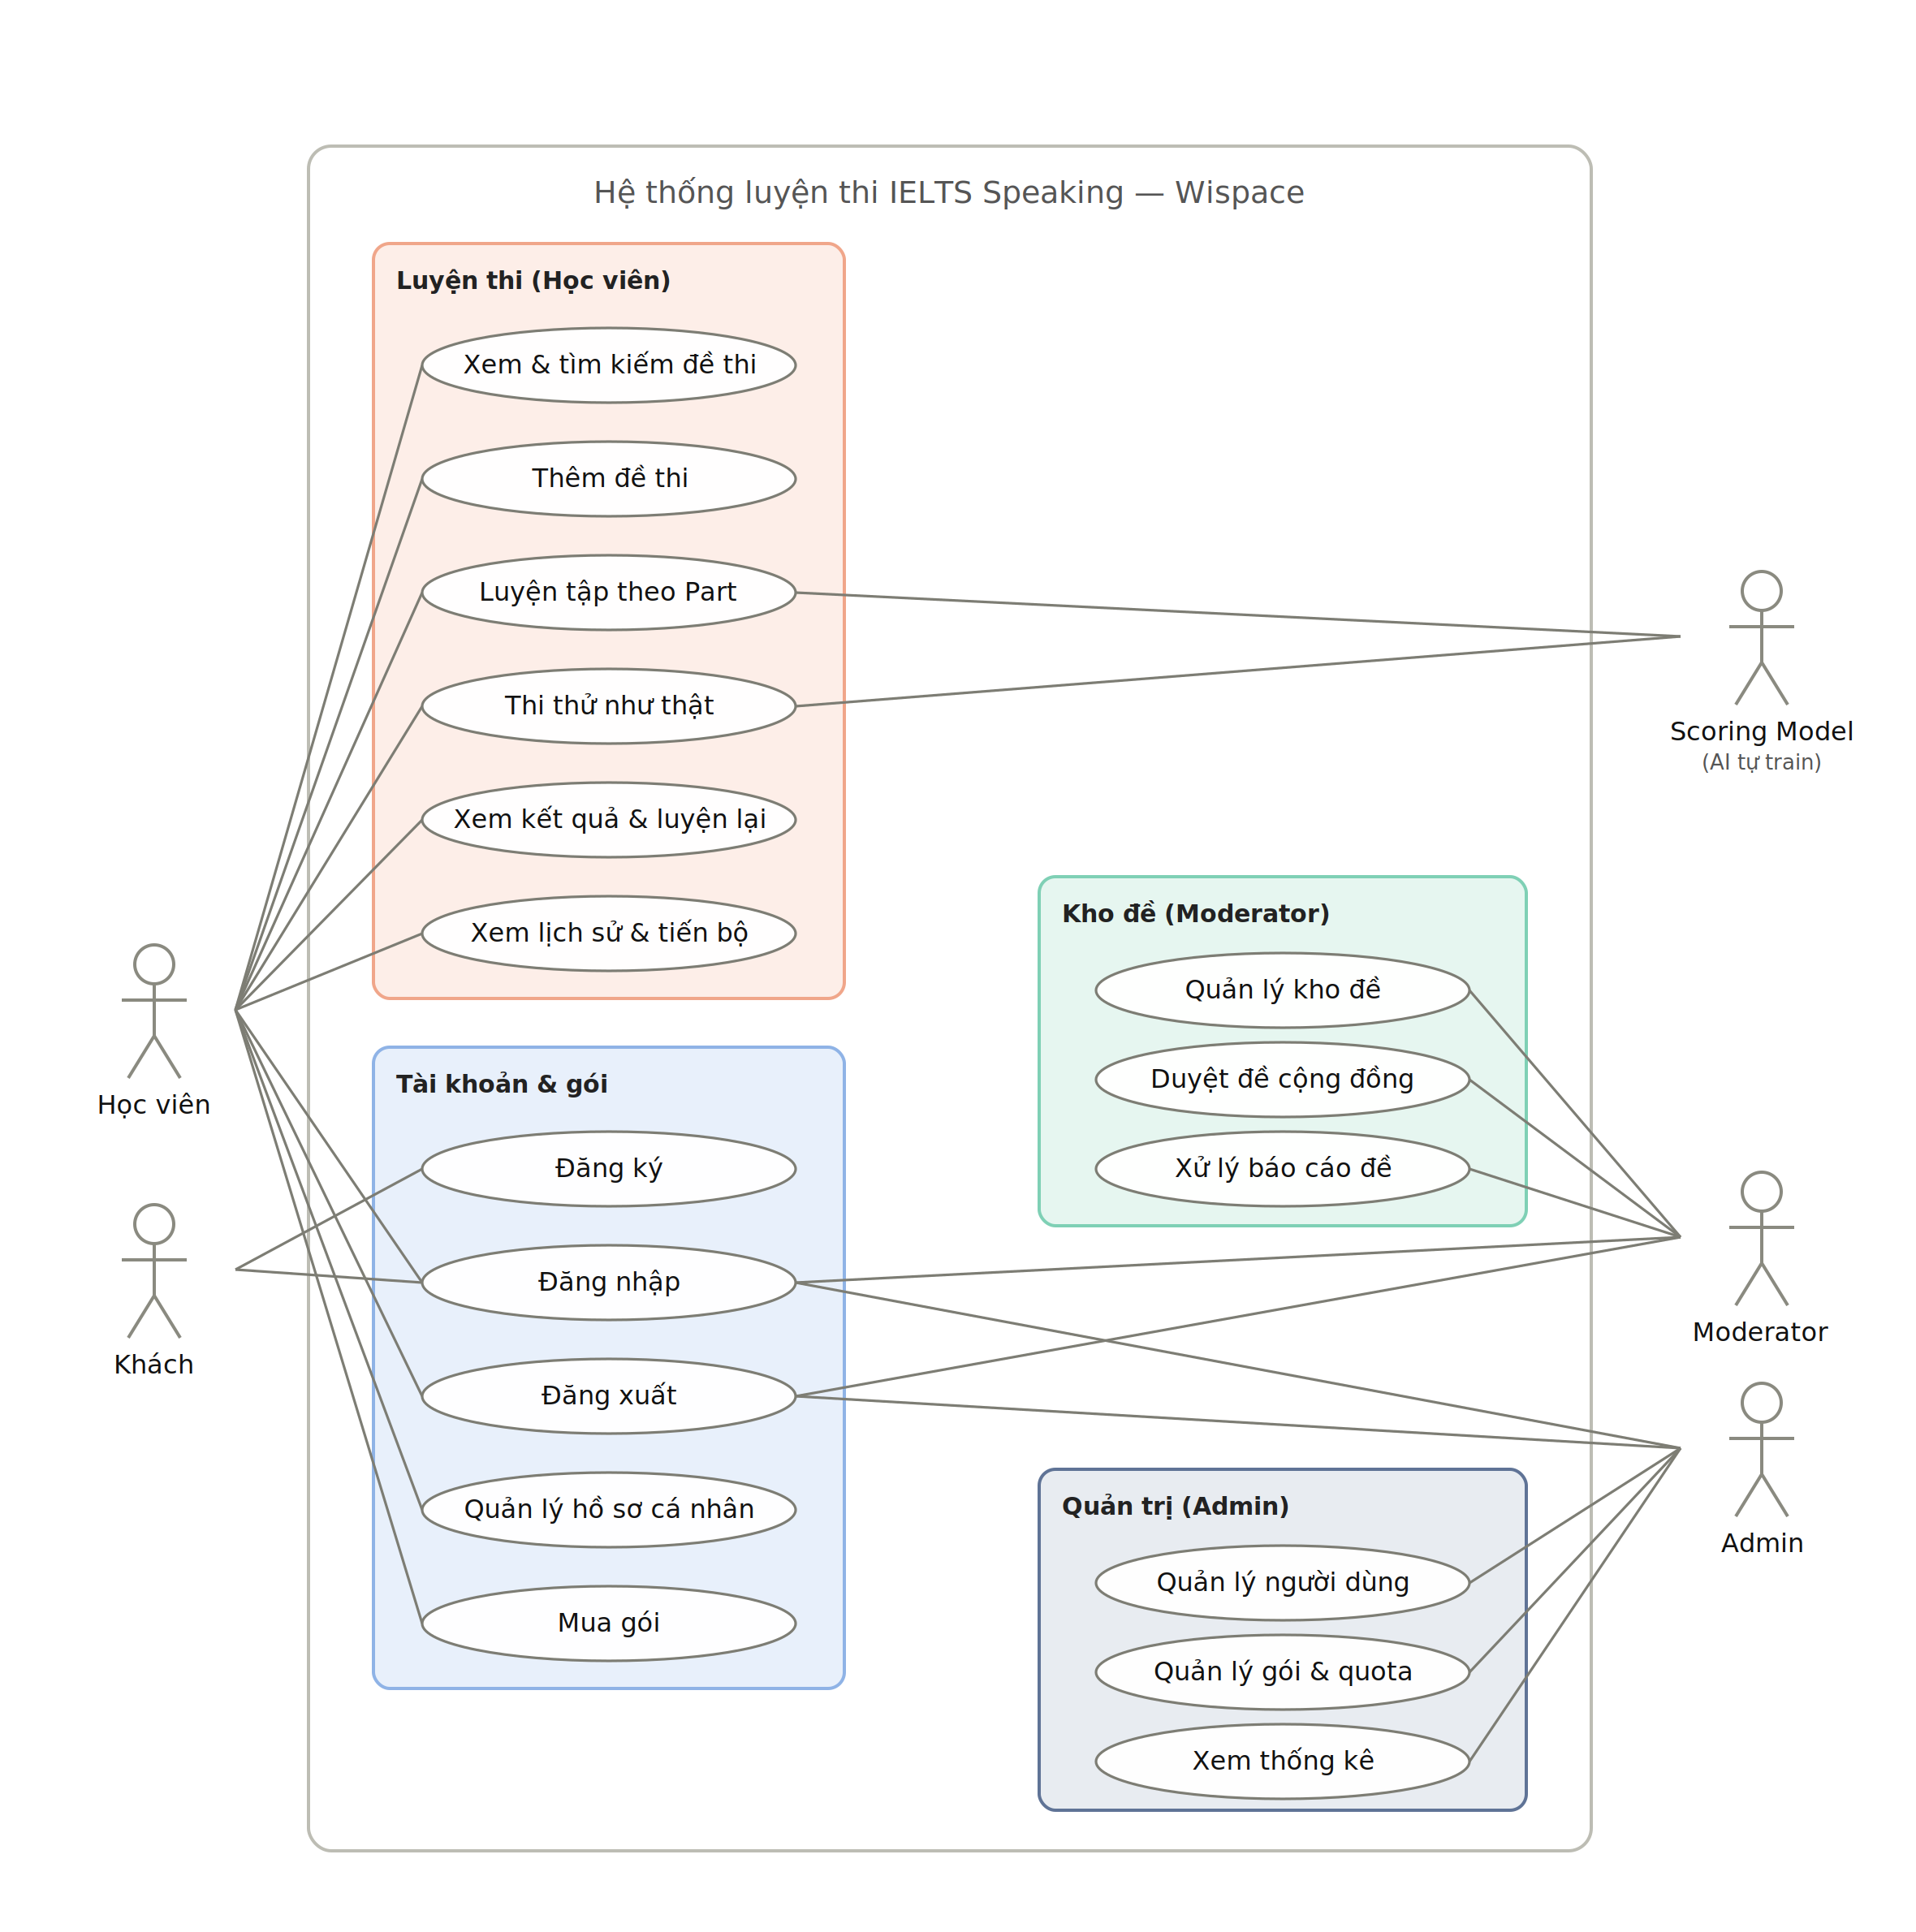
\includegraphics[width=1\textwidth]{Images/Usecase/Wispace/wispace_usecase.jpg}
    \caption{Sơ đồ Use-case tổng quan hệ thống Wispace}
    \label{wispace:fig:wispace_usecase_overview}
\end{figure}
\newpage

\subsubsection{Đặc tả các Use-case chi tiết}
\setcounter{paragraph}{0}
\renewcommand{\theparagraph}{\alph{paragraph}}

Các use-case dưới đây mô tả chi tiết những luồng nghiệp vụ cốt lõi của mô-đun Wispace Speaking, bao gồm quản lý tài khoản, quản lý kho đề, luyện tập, thi thử và theo dõi tiến bộ. Mỗi use-case xác định tác nhân, điều kiện thực hiện, luồng chính, luồng thay thế và các trường hợp ngoại lệ.

\paragraph{Use-case 1: Đăng ký tài khoản}

\begingroup
\small
\renewcommand{\arraystretch}{1.15}
\begin{longtable}{|p{3.2cm}|p{\dimexpr\linewidth-3.2cm-4\tabcolsep-3\arrayrulewidth\relax}|}
\caption{Đặc tả use-case Đăng ký tài khoản}\label{wispace:tab:wispace_uc01_register}\\
\hline
\textbf{Thuộc tính} & \textbf{Nội dung} \\ \hline
\endfirsthead
\multicolumn{2}{c}{\textit{Đặc tả use-case Đăng ký tài khoản (tiếp theo)}}\\
\hline
\textbf{Thuộc tính} & \textbf{Nội dung} \\ \hline
\endhead
\hline
\endfoot
\textbf{Tác nhân} & Khách; Dịch vụ Email; Google OAuth \\ \hline
\textbf{Tiền điều kiện} & \textbullet{}\ Hệ thống hoạt động bình thường.\newline \textbullet{}\ Khách chưa đăng nhập; email chưa tồn tại trong hệ thống. \\ \hline
\textbf{Hậu điều kiện} & \textbullet{}\ Tài khoản ở trạng thái Active, được cấp gói dùng thử.\newline \textbullet{}\ Khách được đăng nhập và chuyển tới trang onboarding. \\ \hline
\textbf{Luồng chính} & 1. Khách nhấn "Đăng ký".\newline 2. Hệ thống hiển thị form đăng ký.\newline 3. Khách nhập email, mật khẩu, xác nhận mật khẩu, nhấn "Đăng ký".\newline 4. Hệ thống kiểm tra dữ liệu, tạo tài khoản chờ xác thực và gửi OTP 6 số qua Dịch vụ Email.\newline 5. Khách nhập OTP.\newline 6. Hệ thống xác thực OTP, kích hoạt tài khoản và cấp gói dùng thử.\newline 7. Hệ thống đăng nhập và chuyển Khách tới trang onboarding. \\ \hline
\textbf{Luồng thay thế} & \textbf{Nhánh 2:} Tại bước 3 --- đăng ký bằng Google\newline 3.1. Khách nhấn "Tiếp tục với Google".\newline 3.2. Google OAuth xác thực và trả về email.\newline 3.3. Hệ thống tạo tài khoản Active, bỏ qua bước 4--6 và sang bước 7. \\ \hline
\textbf{Ngoại lệ} & \textbf{Lỗi 1:} Tại bước 4 --- email đã tồn tại: hệ thống báo lỗi, gợi ý đăng nhập hoặc quên mật khẩu.\newline \textbf{Lỗi 2:} Tại bước 4 --- mật khẩu dưới 8 ký tự hoặc không khớp: báo lỗi tại trường, giữ dữ liệu đã nhập.\newline \textbf{Lỗi 3:} Tại bước 6 --- OTP sai: cho nhập lại; sai 5 lần thì khóa 15 phút.\newline \textbf{Lỗi 4:} Tại bước 6 --- OTP quá 15 phút: Khách nhấn "Gửi lại OTP" (cách nhau tối thiểu 60 giây). \\ \hline
\end{longtable}
\endgroup


\paragraph{Use-case 2: Đăng nhập}

\begingroup
\small
\renewcommand{\arraystretch}{1.15}
\begin{longtable}{|p{3.2cm}|p{\dimexpr\linewidth-3.2cm-4\tabcolsep-3\arrayrulewidth\relax}|}
\caption{Đặc tả use-case Đăng nhập}\label{wispace:tab:wispace_uc02_login}\\
\hline
\textbf{Thuộc tính} & \textbf{Nội dung} \\ \hline
\endfirsthead
\multicolumn{2}{c}{\textit{Đặc tả use-case Đăng nhập (tiếp theo)}}\\
\hline
\textbf{Thuộc tính} & \textbf{Nội dung} \\ \hline
\endhead
\hline
\endfoot
\textbf{Tác nhân} & Học viên, Moderator, Admin; Máy chủ xác thực; Google OAuth \\ \hline
\textbf{Tiền điều kiện} & \textbullet{}\ Hệ thống hoạt động bình thường.\newline \textbullet{}\ Người dùng truy cập trang đăng nhập và đã có tài khoản. \\ \hline
\textbf{Hậu điều kiện} & \textbullet{}\ Người dùng đăng nhập thành công, nhận access token và refresh token.\newline \textbullet{}\ Người dùng được chuyển tới trang chủ theo vai trò. \\ \hline
\textbf{Luồng chính} & 1. Người dùng nhấn "Đăng nhập".\newline 2. Hệ thống hiển thị form đăng nhập.\newline 3. Người dùng nhập email, mật khẩu và nhấn "Đăng nhập".\newline 4. Máy chủ xác thực kiểm tra thông tin và trạng thái tài khoản.\newline 5. Hệ thống cấp token và chuyển trang: Học viên $\rightarrow$ Dashboard Speaking; Moderator $\rightarrow$ Quản lý đề; Admin $\rightarrow$ Trang quản trị.\newline 6. Nếu học viên có bài thi đang dở (dưới 30 phút), hệ thống hỏi "Tiếp tục bài thi" hoặc "Nộp phần đã làm". \\ \hline
\textbf{Luồng thay thế} & \textbf{Nhánh 1:} Tại bước 3 --- quên mật khẩu\newline 3.1. Người dùng nhấn "Quên mật khẩu".\newline 3.2. Hệ thống yêu cầu nhập email.\newline 3.3. Người dùng nhập email.\newline 3.4. Hệ thống gửi OTP đến email.\newline 3.5. Người dùng nhập OTP và mật khẩu mới.\newline 3.6. Hệ thống cập nhật mật khẩu, thu hồi mọi phiên cũ, quay lại bước 1.\newline \textbf{Nhánh 2:} Tại bước 3 --- đăng nhập bằng Google\newline 3.1. Người dùng nhấn "Đăng nhập bằng Google".\newline 3.2. Google OAuth xác thực và trả về email.\newline 3.3. Hệ thống sang bước 5; email chưa có tài khoản thì tự tạo tài khoản học viên. \\ \hline
\textbf{Ngoại lệ} & \textbf{Lỗi 1:} Tại bước 4 --- sai email hoặc mật khẩu: thông báo chung "Email hoặc mật khẩu không đúng"; sai 5 lần thì khóa 15 phút.\newline \textbf{Lỗi 2:} Tại bước 4 --- tài khoản bị khóa: thông báo lý do và cách liên hệ hỗ trợ.\newline \textbf{Lỗi 3:} Tại bước 4 --- tài khoản chưa xác thực OTP: gửi lại OTP và chuyển sang bước 5 của use-case Đăng ký.\newline \textbf{Lỗi 4:} Tại Alternative 1 --- email không tồn tại: vẫn báo "đã gửi mã" để không lộ thông tin tài khoản. \\ \hline
\end{longtable}
\endgroup


\paragraph{Use-case 3: Đăng xuất}

\begingroup
\small
\renewcommand{\arraystretch}{1.15}
\begin{longtable}{|p{3.2cm}|p{\dimexpr\linewidth-3.2cm-4\tabcolsep-3\arrayrulewidth\relax}|}
\caption{Đặc tả use-case Đăng xuất}\label{wispace:tab:wispace_uc03_logout}\\
\hline
\textbf{Thuộc tính} & \textbf{Nội dung} \\ \hline
\endfirsthead
\multicolumn{2}{c}{\textit{Đặc tả use-case Đăng xuất (tiếp theo)}}\\
\hline
\textbf{Thuộc tính} & \textbf{Nội dung} \\ \hline
\endhead
\hline
\endfoot
\textbf{Tác nhân} & Học viên, Moderator, Admin \\ \hline
\textbf{Tiền điều kiện} & Người dùng đã đăng nhập. \\ \hline
\textbf{Hậu điều kiện} & \textbullet{}\ Refresh token bị thu hồi; dữ liệu phiên trên trình duyệt bị xóa.\newline \textbullet{}\ Người dùng ở trang đăng nhập. \\ \hline
\textbf{Luồng chính} & 1. Người dùng nhấn "Đăng xuất".\newline 2. Hệ thống kiểm tra người dùng có đang thi hoặc đang ghi âm không.\newline 3. Hệ thống thu hồi refresh token (đưa vào danh sách chặn).\newline 4. Trình duyệt xóa token và dữ liệu tạm.\newline 5. Hệ thống chuyển về trang đăng nhập. \\ \hline
\textbf{Luồng thay thế} & \textbf{Nhánh 1:} Tại bước 1 --- đăng xuất mọi thiết bị\newline 1.1. Người dùng vào Cài đặt và nhấn "Đăng xuất mọi thiết bị".\newline 1.2. Hệ thống yêu cầu xác nhận bằng mật khẩu.\newline 1.3. Hệ thống đổi Security Stamp; mọi token cũ bị từ chối ở lần gọi tiếp theo; sang bước 4.\newline \textbf{Nhánh 2:} Tại bước 2 --- đang trong phòng thi\newline 2.1. Hệ thống hiển thị hộp thoại: "Nộp phần đã làm và đăng xuất" / "Huỷ bài thi" / "Quay lại".\newline 2.2. Chọn nộp: hệ thống lưu bài, đưa vào hàng chấm và sang bước 3.\newline 2.3. Chọn quay lại: kết thúc use-case, tiếp tục thi. \\ \hline
\textbf{Ngoại lệ} & \textbf{Lỗi 1:} Tại bước 3 --- mất mạng: trình duyệt vẫn xóa token cục bộ; refresh token tự hết hạn.\newline \textbf{Lỗi 2:} Tại bước 2 --- còn audio chưa upload: cảnh báo và chờ upload xong mới đăng xuất. \\ \hline
\end{longtable}
\endgroup


\paragraph{Use-case 4: Quản lý hồ sơ cá nhân}

\begingroup
\small
\renewcommand{\arraystretch}{1.15}
\begin{longtable}{|p{3.2cm}|p{\dimexpr\linewidth-3.2cm-4\tabcolsep-3\arrayrulewidth\relax}|}
\caption{Đặc tả use-case Quản lý hồ sơ cá nhân}\label{wispace:tab:wispace_uc04_profile}\\
\hline
\textbf{Thuộc tính} & \textbf{Nội dung} \\ \hline
\endfirsthead
\multicolumn{2}{c}{\textit{Đặc tả use-case Quản lý hồ sơ cá nhân (tiếp theo)}}\\
\hline
\textbf{Thuộc tính} & \textbf{Nội dung} \\ \hline
\endhead
\hline
\endfoot
\textbf{Tác nhân} & Học viên \\ \hline
\textbf{Tiền điều kiện} & Học viên đã đăng nhập. \\ \hline
\textbf{Hậu điều kiện} & \textbullet{}\ Thông tin hồ sơ được lưu.\newline \textbullet{}\ Band mục tiêu và ngày thi được dùng để cá nhân hoá gợi ý luyện tập. \\ \hline
\textbf{Luồng chính} & 1. Học viên nhấn "Hồ sơ".\newline 2. Hệ thống hiển thị 4 tab: Thông tin, Thiết bị, Gói \& quota, Quyền riêng tư.\newline 3. Học viên sửa tên, avatar, band mục tiêu (5.0--9.0), ngày thi dự kiến, giọng giám khảo (Anh-Anh / Anh-Mỹ / Úc) và nhấn "Lưu".\newline 4. Hệ thống kiểm tra dữ liệu và lưu.\newline 5. Hệ thống thông báo cập nhật thành công. \\ \hline
\textbf{Luồng thay thế} & \textbf{Nhánh 1:} Tại bước 2 --- kiểm tra micro\newline 2.1. Học viên chọn tab Thiết bị, chọn micro và ghi thử 5 giây.\newline 2.2. Hệ thống phát lại và hiển thị mức âm lượng, độ ồn.\newline \textbf{Nhánh 2:} Tại bước 2 --- đổi mật khẩu\newline 2.1. Học viên nhập mật khẩu cũ và mật khẩu mới.\newline 2.2. Hệ thống cập nhật và thu hồi phiên trên các thiết bị khác.\newline \textbf{Nhánh 3:} Tại bước 2 --- xem gói \& quota\newline 2.1. Hệ thống hiển thị gói hiện tại, ngày hết hạn, số phút chấm và lượt thi còn lại hôm nay.\newline 2.2. Học viên nhấn "Nâng cấp" để chuyển sang use-case Mua gói.\newline \textbf{Nhánh 4:} Tại bước 2 --- xóa audio / xóa tài khoản\newline 2.1. Học viên chọn tab Quyền riêng tư, nhấn xóa và xác nhận bằng mật khẩu hoặc OTP.\newline 2.2. Hệ thống xóa audio ngay; với xóa tài khoản, chuyển sang trạng thái Chờ xóa 30 ngày và đăng xuất mọi thiết bị. \\ \hline
\textbf{Ngoại lệ} & \textbf{Lỗi 1:} Tại bước 4 --- ảnh avatar lớn hơn 2 MB hoặc sai định dạng: báo lỗi, không lưu ảnh.\newline \textbf{Lỗi 2:} Tại Alternative 1 --- trình duyệt chặn micro: hướng dẫn cấp quyền theo từng trình duyệt.\newline \textbf{Lỗi 3:} Tại Alternative 2 --- mật khẩu cũ sai: báo lỗi, không đổi mật khẩu. \\ \hline
\end{longtable}
\endgroup


\paragraph{Use-case 5: Quản lý người dùng}

\begingroup
\small
\renewcommand{\arraystretch}{1.15}
\begin{longtable}{|p{3.2cm}|p{\dimexpr\linewidth-3.2cm-4\tabcolsep-3\arrayrulewidth\relax}|}
\caption{Đặc tả use-case Quản lý người dùng}\label{wispace:tab:wispace_uc05_user_management}\\
\hline
\textbf{Thuộc tính} & \textbf{Nội dung} \\ \hline
\endfirsthead
\multicolumn{2}{c}{\textit{Đặc tả use-case Quản lý người dùng (tiếp theo)}}\\
\hline
\textbf{Thuộc tính} & \textbf{Nội dung} \\ \hline
\endhead
\hline
\endfoot
\textbf{Tác nhân} & Admin; Dịch vụ Email \\ \hline
\textbf{Tiền điều kiện} & Admin đã đăng nhập với vai trò Admin. \\ \hline
\textbf{Hậu điều kiện} & \textbullet{}\ Thay đổi có hiệu lực ngay.\newline \textbullet{}\ Mỗi thao tác được ghi nhật ký (người làm, thời điểm, trước/sau, lý do).\newline \textbullet{}\ Người dùng nhận email thông báo. \\ \hline
\textbf{Luồng chính} & 1. Admin mở "Quản lý người dùng".\newline 2. Hệ thống hiển thị danh sách phân trang 20 dòng và bộ lọc.\newline 3. Admin nhập email/tên và lọc theo vai trò, gói, trạng thái, ngày đăng ký.\newline 4. Hệ thống trả kết quả.\newline 5. Admin chọn một người dùng.\newline 6. Hệ thống hiển thị chi tiết: thông tin, gói, lịch sử thanh toán, quota đã dùng 30 ngày, số bài, band trung bình.\newline 7. Admin chọn thao tác (Khóa / mở khóa, Đổi vai trò, Cộng quota), nhập lý do và xác nhận.\newline 8. Hệ thống áp dụng thay đổi, ghi nhật ký và gửi email thông báo qua Dịch vụ Email. \\ \hline
\textbf{Luồng thay thế} & \textbf{Nhánh 1:} Tại bước 7 --- khóa tài khoản\newline 7.1. Hệ thống đổi Security Stamp, người dùng bị đăng xuất ngay.\newline 7.2. Bài thi đang làm (nếu có) được lưu ở trạng thái Đã huỷ.\newline \textbf{Nhánh 2:} Tại bước 7 --- cộng quota thủ công\newline 7.1. Admin nhập số phút chấm hoặc số lượt thi và hạn dùng.\newline 7.2. Hệ thống tạo bản ghi điều chỉnh quota.\newline \textbf{Nhánh 3:} Tại bước 4 --- xuất danh sách\newline 4.1. Admin nhấn "Xuất CSV"; hệ thống tải file theo bộ lọc hiện tại. \\ \hline
\textbf{Ngoại lệ} & \textbf{Lỗi 1:} Tại bước 4 --- không có kết quả: hiển thị "Không tìm thấy người dùng".\newline \textbf{Lỗi 2:} Tại bước 6 --- xem audio của người dùng: chỉ mở khi nhập mã ticket hỗ trợ; hệ thống ghi nhật ký.\newline \textbf{Lỗi 3:} Tại bước 7 --- không nhập lý do: không cho xác nhận.\newline \textbf{Lỗi 4:} Tại bước 7 --- Admin khóa hoặc hạ vai trò chính mình: hệ thống từ chối. \\ \hline
\end{longtable}
\endgroup


\paragraph{Use-case 6: Xem và tìm kiếm đề thi}

\begingroup
\small
\renewcommand{\arraystretch}{1.15}
\begin{longtable}{|p{3.2cm}|p{\dimexpr\linewidth-3.2cm-4\tabcolsep-3\arrayrulewidth\relax}|}
\caption{Đặc tả use-case Xem và tìm kiếm đề thi}\label{wispace:tab:wispace_uc06_browse_tests}\\
\hline
\textbf{Thuộc tính} & \textbf{Nội dung} \\ \hline
\endfirsthead
\multicolumn{2}{c}{\textit{Đặc tả use-case Xem và tìm kiếm đề thi (tiếp theo)}}\\
\hline
\textbf{Thuộc tính} & \textbf{Nội dung} \\ \hline
\endhead
\hline
\endfoot
\textbf{Tác nhân} & Học viên, Khách \\ \hline
\textbf{Tiền điều kiện} & \textbullet{}\ Hệ thống hoạt động bình thường.\newline \textbullet{}\ Kho đề có dữ liệu. \\ \hline
\textbf{Hậu điều kiện} & Người dùng thấy danh sách hoặc chi tiết đề; học viên có thể chuyển sang Luyện tập hoặc Thi thử. \\ \hline
\textbf{Luồng chính} & 1. Người dùng nhấn "Đề thi Speaking".\newline 2. Hệ thống hiển thị các tab nguồn (Cambridge, Forecast, Đề của tôi, Cộng đồng), mặc định Forecast quý hiện tại, 24 thẻ mỗi trang.\newline 3. Người dùng chọn tab, lọc theo Part, chủ đề, trạng thái hoặc nhập từ khoá.\newline 4. Hệ thống trả về các đề phù hợp.\newline 5. Người dùng nhấn vào một thẻ đề.\newline 6. Hệ thống hiển thị chi tiết: câu hỏi từng Part, số lượt luyện, band cao nhất của học viên, nút "Luyện tập" và "Thi thử". \\ \hline
\textbf{Luồng thay thế} & \textbf{Nhánh 1:} Tại bước 3 --- chọn tab Cambridge\newline 3.1. Hệ thống hiển thị lưới quyển Cambridge IELTS 1--20.\newline 3.2. Người dùng chọn quyển; hệ thống hiển thị Test 1--4 của quyển đó, sang bước 5.\newline \textbf{Nhánh 2:} Tại bước 6 --- đánh dấu yêu thích\newline 6.1. Học viên nhấn biểu tượng ngôi sao; hệ thống lưu đề vào danh sách Yêu thích.\newline \textbf{Nhánh 3:} Tại bước 6 --- báo cáo đề sai\newline 6.1. Học viên chọn lý do (sai nội dung, trùng, không phù hợp) và gửi.\newline 6.2. Hệ thống đưa báo cáo vào hàng chờ của Moderator. \\ \hline
\textbf{Ngoại lệ} & \textbf{Lỗi 1:} Tại bước 4 --- không có kết quả: gợi ý bỏ bớt bộ lọc hoặc "Thêm đề này".\newline \textbf{Lỗi 2:} Tại bước 6 --- Khách nhấn Luyện tập / Thi thử: chuyển sang use-case Đăng nhập.\newline \textbf{Lỗi 3:} Tại bước 6 --- đề thuộc gói trả phí, học viên dùng gói miễn phí: hiển thị màn hình nâng cấp gói.\newline \textbf{Lỗi 4:} Tại bước 3 --- tab Đề của tôi trống: hiển thị nút "Thêm đề đầu tiên". \\ \hline
\end{longtable}
\endgroup


\paragraph{Use-case 7: Thêm đề thi}

\begingroup
\small
\renewcommand{\arraystretch}{1.15}
\begin{longtable}{|p{3.2cm}|p{\dimexpr\linewidth-3.2cm-4\tabcolsep-3\arrayrulewidth\relax}|}
\caption{Đặc tả use-case Thêm đề thi}\label{wispace:tab:wispace_uc07_add_test}\\
\hline
\textbf{Thuộc tính} & \textbf{Nội dung} \\ \hline
\endfirsthead
\multicolumn{2}{c}{\textit{Đặc tả use-case Thêm đề thi (tiếp theo)}}\\
\hline
\textbf{Thuộc tính} & \textbf{Nội dung} \\ \hline
\endhead
\hline
\endfoot
\textbf{Tác nhân} & Học viên; AI hỗ trợ \\ \hline
\textbf{Tiền điều kiện} & \textbullet{}\ Học viên đã đăng nhập.\newline \textbullet{}\ Chưa vượt giới hạn số đề (gói miễn phí 10 đề, gói trả phí 200 đề). \\ \hline
\textbf{Hậu điều kiện} & \textbullet{}\ Đề được lưu ở chế độ Riêng tư, nguồn "Học viên tạo".\newline \textbullet{}\ Đề hiển thị trong tab Đề của tôi và luyện được ngay. \\ \hline
\textbf{Luồng chính} & 1. Học viên nhấn "+ Thêm đề".\newline 2. Hệ thống hiển thị form chọn loại đề: Part 1, Part 2 (kèm Part 3), Full test.\newline 3. Học viên nhập nội dung (Part 1: chủ đề + 3--6 câu; Part 2: cue card + 3--4 gợi ý; Part 3: 4--6 câu thảo luận), gắn chủ đề, nguồn tham khảo và nhấn "Lưu".\newline 4. Hệ thống kiểm tra hợp lệ: mỗi câu tối đa 300 ký tự, bằng tiếng Anh, lọc từ ngữ không phù hợp, loại bỏ mã HTML.\newline 5. Hệ thống kiểm tra trùng lặp với kho đề.\newline 6. Hệ thống lưu đề và hiển thị nút "Luyện ngay" và "Đề xuất công khai". \\ \hline
\textbf{Luồng thay thế} & \textbf{Nhánh 1:} Tại bước 3 --- AI gợi ý câu Part 3\newline 3.1. Học viên nhập cue card Part 2 và nhấn "Gợi ý Part 3".\newline 3.2. AI hỗ trợ sinh 5 câu Part 3 liên quan.\newline 3.3. Học viên giữ hoặc bỏ từng câu, quay lại bước 3.\newline \textbf{Nhánh 2:} Tại bước 5 --- đề gần giống đề có sẵn (từ 90\%)\newline 5.1. Hệ thống hiển thị đề có sẵn.\newline 5.2. Học viên chọn "Dùng đề có sẵn" (kết thúc) hoặc "Vẫn lưu" (sang bước 6).\newline \textbf{Nhánh 3:} Tại bước 6 --- đề xuất công khai\newline 6.1. Học viên nhấn "Đề xuất công khai".\newline 6.2. Hệ thống chuyển đề sang trạng thái Chờ duyệt và đưa vào hàng chờ Moderator (use-case 5.8). \\ \hline
\textbf{Ngoại lệ} & \textbf{Lỗi 1:} Tại bước 1 --- vượt giới hạn số đề: thông báo và gợi ý nâng cấp gói.\newline \textbf{Lỗi 2:} Tại bước 4 --- dữ liệu không hợp lệ: báo lỗi đúng trường, giữ dữ liệu đã nhập.\newline \textbf{Lỗi 3:} Tại Alternative 1 --- AI lỗi hoặc quá 30 giây: báo lỗi, học viên tự nhập Part 3. \\ \hline
\end{longtable}
\endgroup


\paragraph{Use-case 8: Quản lý và duyệt kho đề}

\begingroup
\small
\renewcommand{\arraystretch}{1.15}
\begin{longtable}{|p{3.2cm}|p{\dimexpr\linewidth-3.2cm-4\tabcolsep-3\arrayrulewidth\relax}|}
\caption{Đặc tả use-case Quản lý và duyệt kho đề}\label{wispace:tab:wispace_uc08_moderate_tests}\\
\hline
\textbf{Thuộc tính} & \textbf{Nội dung} \\ \hline
\endfirsthead
\multicolumn{2}{c}{\textit{Đặc tả use-case Quản lý và duyệt kho đề (tiếp theo)}}\\
\hline
\textbf{Thuộc tính} & \textbf{Nội dung} \\ \hline
\endhead
\hline
\endfoot
\textbf{Tác nhân} & Moderator; Dịch vụ TTS \\ \hline
\textbf{Tiền điều kiện} & Người dùng đã đăng nhập với vai trò Moderator hoặc Admin. \\ \hline
\textbf{Hậu điều kiện} & \textbullet{}\ Kho đề được cập nhật; đề mới có sẵn audio câu hỏi.\newline \textbullet{}\ Tác giả đề cộng đồng nhận thông báo kết quả duyệt. \\ \hline
\textbf{Luồng chính} & 1. Moderator mở "Quản lý đề".\newline 2. Hệ thống hiển thị cây Quyển $\rightarrow$ Test $\rightarrow$ Part $\rightarrow$ Câu hỏi và hàng chờ duyệt.\newline 3. Moderator nhấn "Thêm đề", chọn Quyển/Test, nhập câu hỏi từng Part và nhấn "Lưu".\newline 4. Hệ thống kiểm tra hợp lệ và lưu đề.\newline 5. Hệ thống gửi câu hỏi tới Dịch vụ TTS để sinh audio 3 giọng (Anh-Anh, Anh-Mỹ, Úc) và lưu lại để dùng chung.\newline 6. Hệ thống hiển thị đề trên trang đề thi. \\ \hline
\textbf{Luồng thay thế} & \textbf{Nhánh 1:} Tại bước 3 --- nhập file\newline 3.1. Moderator tải lên file CSV/JSON theo mẫu.\newline 3.2. Hệ thống kiểm tra từng dòng; có lỗi thì báo dòng lỗi và không nhập phần nào; hợp lệ thì sang bước 5.\newline \textbf{Nhánh 2:} Tại bước 3 --- tạo bộ Forecast quý\newline 3.1. Moderator chọn các đề Part 1/2/3 và đặt thời gian hiệu lực (ví dụ 01/09--31/12/2026).\newline 3.2. Hệ thống lưu bộ Forecast và sang bước 6.\newline \textbf{Nhánh 3:} Tại bước 2 --- duyệt đề cộng đồng\newline 2.1. Moderator mở một đề chờ duyệt; hệ thống hiển thị kèm các đề tương tự.\newline 2.2. Moderator chọn Duyệt (có thể sửa chính tả, gắn tag), Từ chối (bắt buộc ghi lý do) hoặc Gộp trùng.\newline 2.3. Hệ thống cập nhật trạng thái đề và thông báo cho tác giả.\newline \textbf{Nhánh 4:} Tại bước 2 --- xử lý báo cáo đề\newline 2.1. Moderator mở báo cáo và chọn Gỡ đề, Sửa đề hoặc Bỏ qua.\newline 2.2. Tác giả bị gỡ từ 3 đề trong 30 ngày thì bị tạm khóa quyền đề xuất 30 ngày và Admin nhận thông báo. \\ \hline
\textbf{Ngoại lệ} & \textbf{Lỗi 1:} Tại bước 4 --- thiếu câu hỏi bắt buộc: báo lỗi, không lưu.\newline \textbf{Lỗi 2:} Tại bước 5 --- Dịch vụ TTS lỗi: đề vẫn được lưu, đánh dấu "Thiếu audio" và tự sinh lại sau.\newline \textbf{Lỗi 3:} Tại bước 3 --- ẩn đề đã có bài làm: đề không còn trong danh sách nhưng lịch sử bài của học viên vẫn xem được. \\ \hline
\end{longtable}
\endgroup


\paragraph{Use-case 9: Luyện tập theo Part}

\begingroup
\small
\renewcommand{\arraystretch}{1.15}
\begin{longtable}{|p{3.2cm}|p{\dimexpr\linewidth-3.2cm-4\tabcolsep-3\arrayrulewidth\relax}|}
\caption{Đặc tả use-case Luyện tập theo Part}\label{wispace:tab:wispace_uc09_part_practice}\\
\hline
\textbf{Thuộc tính} & \textbf{Nội dung} \\ \hline
\endfirsthead
\multicolumn{2}{c}{\textit{Đặc tả use-case Luyện tập theo Part (tiếp theo)}}\\
\hline
\textbf{Thuộc tính} & \textbf{Nội dung} \\ \hline
\endhead
\hline
\endfoot
\textbf{Tác nhân} & Học viên; Scoring Model (AI chấm tự train) \\ \hline
\textbf{Tiền điều kiện} & \textbullet{}\ Học viên đã đăng nhập và đã cấp quyền micro.\newline \textbullet{}\ Còn quota phút chấm trong ngày. \\ \hline
\textbf{Hậu điều kiện} & \textbullet{}\ Bài làm, audio, transcript và kết quả được lưu.\newline \textbullet{}\ Quota bị trừ theo số giây audio; sự kiện luyện tập được gửi tới hệ thống thống kê. \\ \hline
\textbf{Luồng chính} & 1. Học viên nhấn "Luyện tập".\newline 2. Hệ thống kiểm tra quota và tạo phiên luyện tập.\newline 3. Hệ thống hiển thị câu hỏi (chữ và nút nghe).\newline 4. Học viên nhấn ghi âm (hoặc phím Space) và trả lời; hệ thống ghi và tải audio lên theo từng đoạn.\newline 5. Học viên nhấn dừng, nghe lại và nhấn "Nộp".\newline 6. Hệ thống gửi audio tới Scoring Model; model trả transcript, lỗi phát âm từng từ và band 4 tiêu chí.\newline 7. Hệ thống hiển thị trạng thái "Đang phân tích" $\rightarrow$ "Đang chấm" $\rightarrow$ kết quả (use-case 5.10).\newline 8. Học viên chuyển sang câu tiếp theo. \\ \hline
\textbf{Luồng thay thế} & \textbf{Nhánh 1:} Tại bước 3 --- nghe câu hỏi\newline 3.1. Học viên nhấn biểu tượng loa; hệ thống phát audio câu hỏi; có thể ẩn chữ để luyện nghe.\newline \textbf{Nhánh 2:} Tại bước 3 --- câu hỏi Part 2\newline 3.1. Hệ thống hiển thị cue card, giấy nháp và đếm 60 giây chuẩn bị.\newline 3.2. Hết 60 giây (hoặc nhấn "Bắt đầu nói sớm"), hệ thống tự ghi âm tối đa 120 giây, sang bước 5.\newline \textbf{Nhánh 3:} Tại bước 5 --- ghi lại\newline 5.1. Học viên nhấn "Ghi lại"; bản cũ bị thay, không trừ quota; quay lại bước 4. \\ \hline
\textbf{Ngoại lệ} & \textbf{Lỗi 1:} Tại bước 2 --- hết quota: hiển thị số phút đã dùng, giờ reset và nút nâng cấp; vẫn cho ghi âm tự nghe nhưng không chấm.\newline \textbf{Lỗi 2:} Tại bước 4 --- micro bị chặn: hướng dẫn cấp quyền; nói quá 3 phút (Part 1/3) thì tự dừng.\newline \textbf{Lỗi 3:} Tại bước 5 --- audio dưới 3 giây hoặc im lặng hơn 80\%: không cho nộp, báo "Không nghe rõ câu trả lời".\newline \textbf{Lỗi 4:} Tại bước 6 --- phần lớn nói tiếng Việt: không chấm, hoàn quota.\newline \textbf{Lỗi 5:} Tại bước 6 --- AI lỗi hoặc quá 60 giây: thực thi tối đa 3 lần (gồm lần đầu); vẫn lỗi thì đánh dấu Thất bại, hoàn quota và cho nhấn "Chấm lại". \\ \hline
\end{longtable}
\endgroup


\paragraph{Use-case 10: Xem kết quả và luyện lại}

\begingroup
\small
\renewcommand{\arraystretch}{1.15}
\begin{longtable}{|p{3.2cm}|p{\dimexpr\linewidth-3.2cm-4\tabcolsep-3\arrayrulewidth\relax}|}
\caption{Đặc tả use-case Xem kết quả và luyện lại}\label{wispace:tab:wispace_uc10_results_retry}\\
\hline
\textbf{Thuộc tính} & \textbf{Nội dung} \\ \hline
\endfirsthead
\multicolumn{2}{c}{\textit{Đặc tả use-case Xem kết quả và luyện lại (tiếp theo)}}\\
\hline
\textbf{Thuộc tính} & \textbf{Nội dung} \\ \hline
\endhead
\hline
\endfoot
\textbf{Tác nhân} & Học viên \\ \hline
\textbf{Tiền điều kiện} & \textbullet{}\ Học viên đã đăng nhập.\newline \textbullet{}\ Câu trả lời đã được chấm thành công. \\ \hline
\textbf{Hậu điều kiện} & Học viên thấy kết quả; nếu luyện lại, lượt mới được lưu và so sánh với lượt trước. \\ \hline
\textbf{Luồng chính} & 1. Học viên mở trang kết quả.\newline 2. Hệ thống hiển thị band tổng và 4 thẻ tiêu chí (FC, LR, GRA, P): điểm, lý do, điểm mạnh, điểm cần cải thiện.\newline 3. Hệ thống hiển thị transcript tô màu lỗi ngữ pháp, từ vựng, phát âm và chỉ số trôi chảy (số từ/phút, số lần ngập ngừng, từ đệm).\newline 4. Học viên đọc nhận xét và gợi ý bước tiếp theo. \\ \hline
\textbf{Luồng thay thế} & \textbf{Nhánh 1:} Tại bước 3 --- nghe lại từ phát âm sai\newline 3.1. Học viên nhấn vào từ được tô.\newline 3.2. Hệ thống phát đoạn audio của học viên, sau đó phát âm chuẩn kèm phiên âm IPA.\newline \textbf{Nhánh 2:} Tại bước 4 --- xem câu trả lời mẫu\newline 4.1. Hệ thống hiển thị câu trả lời band 7.0+ viết lại từ ý của học viên và danh sách từ vựng nâng cấp.\newline \textbf{Nhánh 3:} Tại bước 4 --- luyện lại câu này\newline 4.1. Học viên nhấn "Luyện lại câu này"; hệ thống chuyển sang use-case 5.9 với cùng câu hỏi.\newline 4.2. Chấm xong, hệ thống hiển thị so sánh lần trước và lần này theo 4 tiêu chí.\newline \textbf{Nhánh 4:} Tại bước 4 --- thêm lỗi vào Roadmap\newline 4.1. Lỗi lặp lại từ 3 lần trong 14 ngày, hệ thống gợi ý "Thêm vào Roadmap".\newline 4.2. Học viên đồng ý; lỗi được thêm thành một chương luyện tập. \\ \hline
\textbf{Ngoại lệ} & \textbf{Lỗi 1:} Tại bước 1 --- bài đang chấm: hiển thị trạng thái chờ và tự cập nhật khi xong.\newline \textbf{Lỗi 2:} Tại bước 1 --- chấm thất bại: hiển thị lý do và nút "Chấm lại" (không trừ quota).\newline \textbf{Lỗi 3:} Tại Alternative 1 --- audio đã bị xóa theo chính sách 180 ngày: chỉ hiển thị transcript và phát âm chuẩn.\newline \textbf{Lỗi 4:} Tại Alternative 3 --- hết quota: xử lý như Lỗi 1 của use-case 5.9. \\ \hline
\end{longtable}
\endgroup


\paragraph{Use-case 11: Thi thử như thật}

\begingroup
\small
\renewcommand{\arraystretch}{1.15}
\begin{longtable}{|p{3.2cm}|p{\dimexpr\linewidth-3.2cm-4\tabcolsep-3\arrayrulewidth\relax}|}
\caption{Đặc tả use-case Thi thử như thật}\label{wispace:tab:wispace_uc11_mock_test}\\
\hline
\textbf{Thuộc tính} & \textbf{Nội dung} \\ \hline
\endfirsthead
\multicolumn{2}{c}{\textit{Đặc tả use-case Thi thử như thật (tiếp theo)}}\\
\hline
\textbf{Thuộc tính} & \textbf{Nội dung} \\ \hline
\endhead
\hline
\endfoot
\textbf{Tác nhân} & Học viên; Giám khảo AI; Scoring Model (AI chấm tự train) \\ \hline
\textbf{Tiền điều kiện} & \textbullet{}\ Học viên đã đăng nhập, còn lượt thi thử hôm nay.\newline \textbullet{}\ Không có phiên thi khác đang mở; thiết bị có micro. \\ \hline
\textbf{Hậu điều kiện} & \textbullet{}\ Mọi câu trả lời được lưu; bài chuyển sang Đã nộp và vào hàng chấm; trừ 1 lượt thi.\newline \textbullet{}\ Học viên nhận thông báo khi có báo cáo. \\ \hline
\textbf{Luồng chính} & 1. Học viên chọn đề và nhấn "Thi thử".\newline 2. Hệ thống hiển thị quy chế (không nghe lại, không ghi lại, không tạm dừng; khuyến nghị tai nghe) và xin đồng ý xử lý giọng nói ở lần đầu.\newline 3. Hệ thống kiểm tra thiết bị: chỉnh loa, đọc câu mẫu 5 giây để đo âm lượng và độ ồn, đo mạng.\newline 4. Học viên nhấn "Bắt đầu thi"; hệ thống tạo phiên thi, trừ 1 lượt và tải trước audio câu hỏi.\newline 5. Part 1 (4--5 phút): giám khảo AI đọc từng câu; hệ thống tự ghi âm khi giám khảo nói xong và chuyển câu khi học viên im lặng từ 3 giây hoặc hết 45 giây.\newline 6. Part 2: hệ thống hiển thị cue card và giấy nháp, đếm 60 giây chuẩn bị; giám khảo mời bắt đầu; ghi âm tối đa 120 giây rồi ngắt.\newline 7. Part 3 (4--5 phút): giám khảo hỏi 4--6 câu thảo luận liên quan đến Part 2.\newline 8. Giám khảo kết thúc; hệ thống kiểm tra mọi audio đã tải lên, chuyển bài sang Đã nộp và đưa vào hàng chấm.\newline 9. Scoring Model chấm từng câu và cả bài; hệ thống tạo báo cáo và thông báo qua ứng dụng và email. \\ \hline
\textbf{Luồng thay thế} & \textbf{Nhánh 1:} Tại bước 1 --- thi ngẫu nhiên\newline 1.1. Hệ thống ghép Part 1 + Part 2 + Part 3 cùng chủ đề từ kho đề, sang bước 2.\newline \textbf{Nhánh 2:} Tại bước 5--7 --- xin nhắc lại câu hỏi\newline 5.1. Học viên nhấn "Xin nhắc lại câu hỏi" hoặc nói "Sorry, could you repeat?".\newline 5.2. Giám khảo đọc lại 1 lần, không trừ thời gian.\newline \textbf{Nhánh 3:} Tại bước 6 --- nói dưới 60 giây rồi im lặng từ 5 giây\newline 6.1. Giám khảo hỏi gợi mở "Can you tell me more?" như thi thật.\newline \textbf{Nhánh 4:} Tại bước 5--7 --- kết thúc sớm\newline 5.1. Học viên nhấn "Kết thúc" và xác nhận.\newline 5.2. Hệ thống nộp phần đã làm, sang bước 8; báo cáo chỉ có band từng Part. \\ \hline
\textbf{Ngoại lệ} & \textbf{Lỗi 1:} Tại bước 3 --- không có micro hoặc không cấp quyền: không cho vào thi.\newline \textbf{Lỗi 2:} Tại bước 3 --- ồn nền cao hoặc mic nhỏ: cảnh báo, cho "Vẫn tiếp tục" và đánh dấu chất lượng âm thanh thấp.\newline \textbf{Lỗi 3:} Tại bước 4 --- hết lượt thi: hiển thị màn hình nâng cấp, gợi ý luyện từng Part.\newline \textbf{Lỗi 4:} Tại bước 5--7 --- mất mạng: tiếp tục ghi vào bộ nhớ trình duyệt, tải bù khi có mạng lại.\newline \textbf{Lỗi 5:} Tại bước 5--7 --- tải lại trang hoặc đóng tab: cảnh báo rời trang; quay lại trong 30 phút thì tiếp tục từ câu chưa trả lời, quá 30 phút thì tự nộp phần đã làm.\newline \textbf{Lỗi 6:} Tại bước 9 --- chấm lỗi sau 3 lần thử: bài ở trạng thái Thất bại, hoàn lượt thi và báo Admin. \\ \hline
\end{longtable}
\endgroup


\paragraph{Use-case 12: Xem lịch sử và tiến bộ}

\begingroup
\small
\renewcommand{\arraystretch}{1.15}
\begin{longtable}{|p{3.2cm}|p{\dimexpr\linewidth-3.2cm-4\tabcolsep-3\arrayrulewidth\relax}|}
\caption{Đặc tả use-case Xem lịch sử và tiến bộ}\label{wispace:tab:wispace_uc12_progress_history}\\
\hline
\textbf{Thuộc tính} & \textbf{Nội dung} \\ \hline
\endfirsthead
\multicolumn{2}{c}{\textit{Đặc tả use-case Xem lịch sử và tiến bộ (tiếp theo)}}\\
\hline
\textbf{Thuộc tính} & \textbf{Nội dung} \\ \hline
\endhead
\hline
\endfoot
\textbf{Tác nhân} & Học viên \\ \hline
\textbf{Tiền điều kiện} & Học viên đã đăng nhập. \\ \hline
\textbf{Hậu điều kiện} & Học viên thấy danh sách bài, biểu đồ band và top lỗi; có thể mở lại báo cáo bất kỳ. \\ \hline
\textbf{Luồng chính} & 1. Học viên nhấn "Lịch sử \& tiến bộ".\newline 2. Hệ thống hiển thị biểu đồ band tổng và 4 tiêu chí theo thời gian (mặc định 30 ngày).\newline 3. Hệ thống hiển thị top 5 lỗi lặp lại (từ phát âm sai, cấu trúc ngữ pháp, từ đệm).\newline 4. Hệ thống hiển thị danh sách bài đã làm (luyện tập và thi thử), mới nhất trước, 20 bài mỗi trang.\newline 5. Học viên nhấn vào một bài.\newline 6. Hệ thống mở báo cáo bài (use-case 5.10 với bài luyện tập, báo cáo thi thử với bài thi). \\ \hline
\textbf{Luồng thay thế} & \textbf{Nhánh 1:} Tại bước 4 --- lọc bài\newline 4.1. Học viên chọn Part, nguồn đề, loại bài, khoảng ngày.\newline 4.2. Hệ thống cập nhật danh sách và biểu đồ theo bộ lọc.\newline \textbf{Nhánh 2:} Tại bước 6 --- chia sẻ kết quả\newline 6.1. Học viên nhấn "Chia sẻ".\newline 6.2. Hệ thống tạo link công khai chỉ chứa điểm và nhận xét (không kèm audio); học viên có thể thu hồi link. \\ \hline
\textbf{Ngoại lệ} & \textbf{Lỗi 1:} Tại bước 2 --- chưa có bài nào: hiển thị hướng dẫn và nút "Luyện câu đầu tiên".\newline \textbf{Lỗi 2:} Tại bước 2 --- dưới 3 bài: ẩn biểu đồ xu hướng, chỉ hiển thị điểm từng bài.\newline \textbf{Lỗi 3:} Tại bước 6 --- bài đang chấm hoặc chấm lỗi: hiển thị trạng thái tương ứng (như Lỗi 1--2 của use-case 5.10). \\ \hline
\end{longtable}
\endgroup
\titleformat{\paragraph}[hang]
    {\normalfont\normalsize\bfseries}
    {\theparagraph}{1em}{}


\subsubsection{Luồng hoạt động của hệ thống}

\label{wispace:subsubsec:operational_flows}

\setcounter{paragraph}{0}

Các luồng hoạt động của Wispace Speaking bao gồm quản lý tài khoản, quản lý kho đề, luyện tập, thi thử và theo dõi tiến bộ. Mỗi luồng trình bày thao tác của người dùng, quá trình xử lý của hệ thống và kết quả nhận được, đồng thời xác định cách xử lý khi dữ liệu không hợp lệ hoặc phát sinh lỗi.

Các luồng luyện tập và thi thử sử dụng hàng đợi chấm bất đồng bộ; việc lưu bài, giữ quota, ghi nhận kết quả hoặc hoàn quota khi thất bại phải bảo đảm nhất quán và không thực hiện lặp khi thử lại.

\clearpage

\paragraph{Luồng hoạt động: Đăng ký tài khoản (Use-case 1)}

% activity-generated:start
\begin{figure}[H]
    \centering
    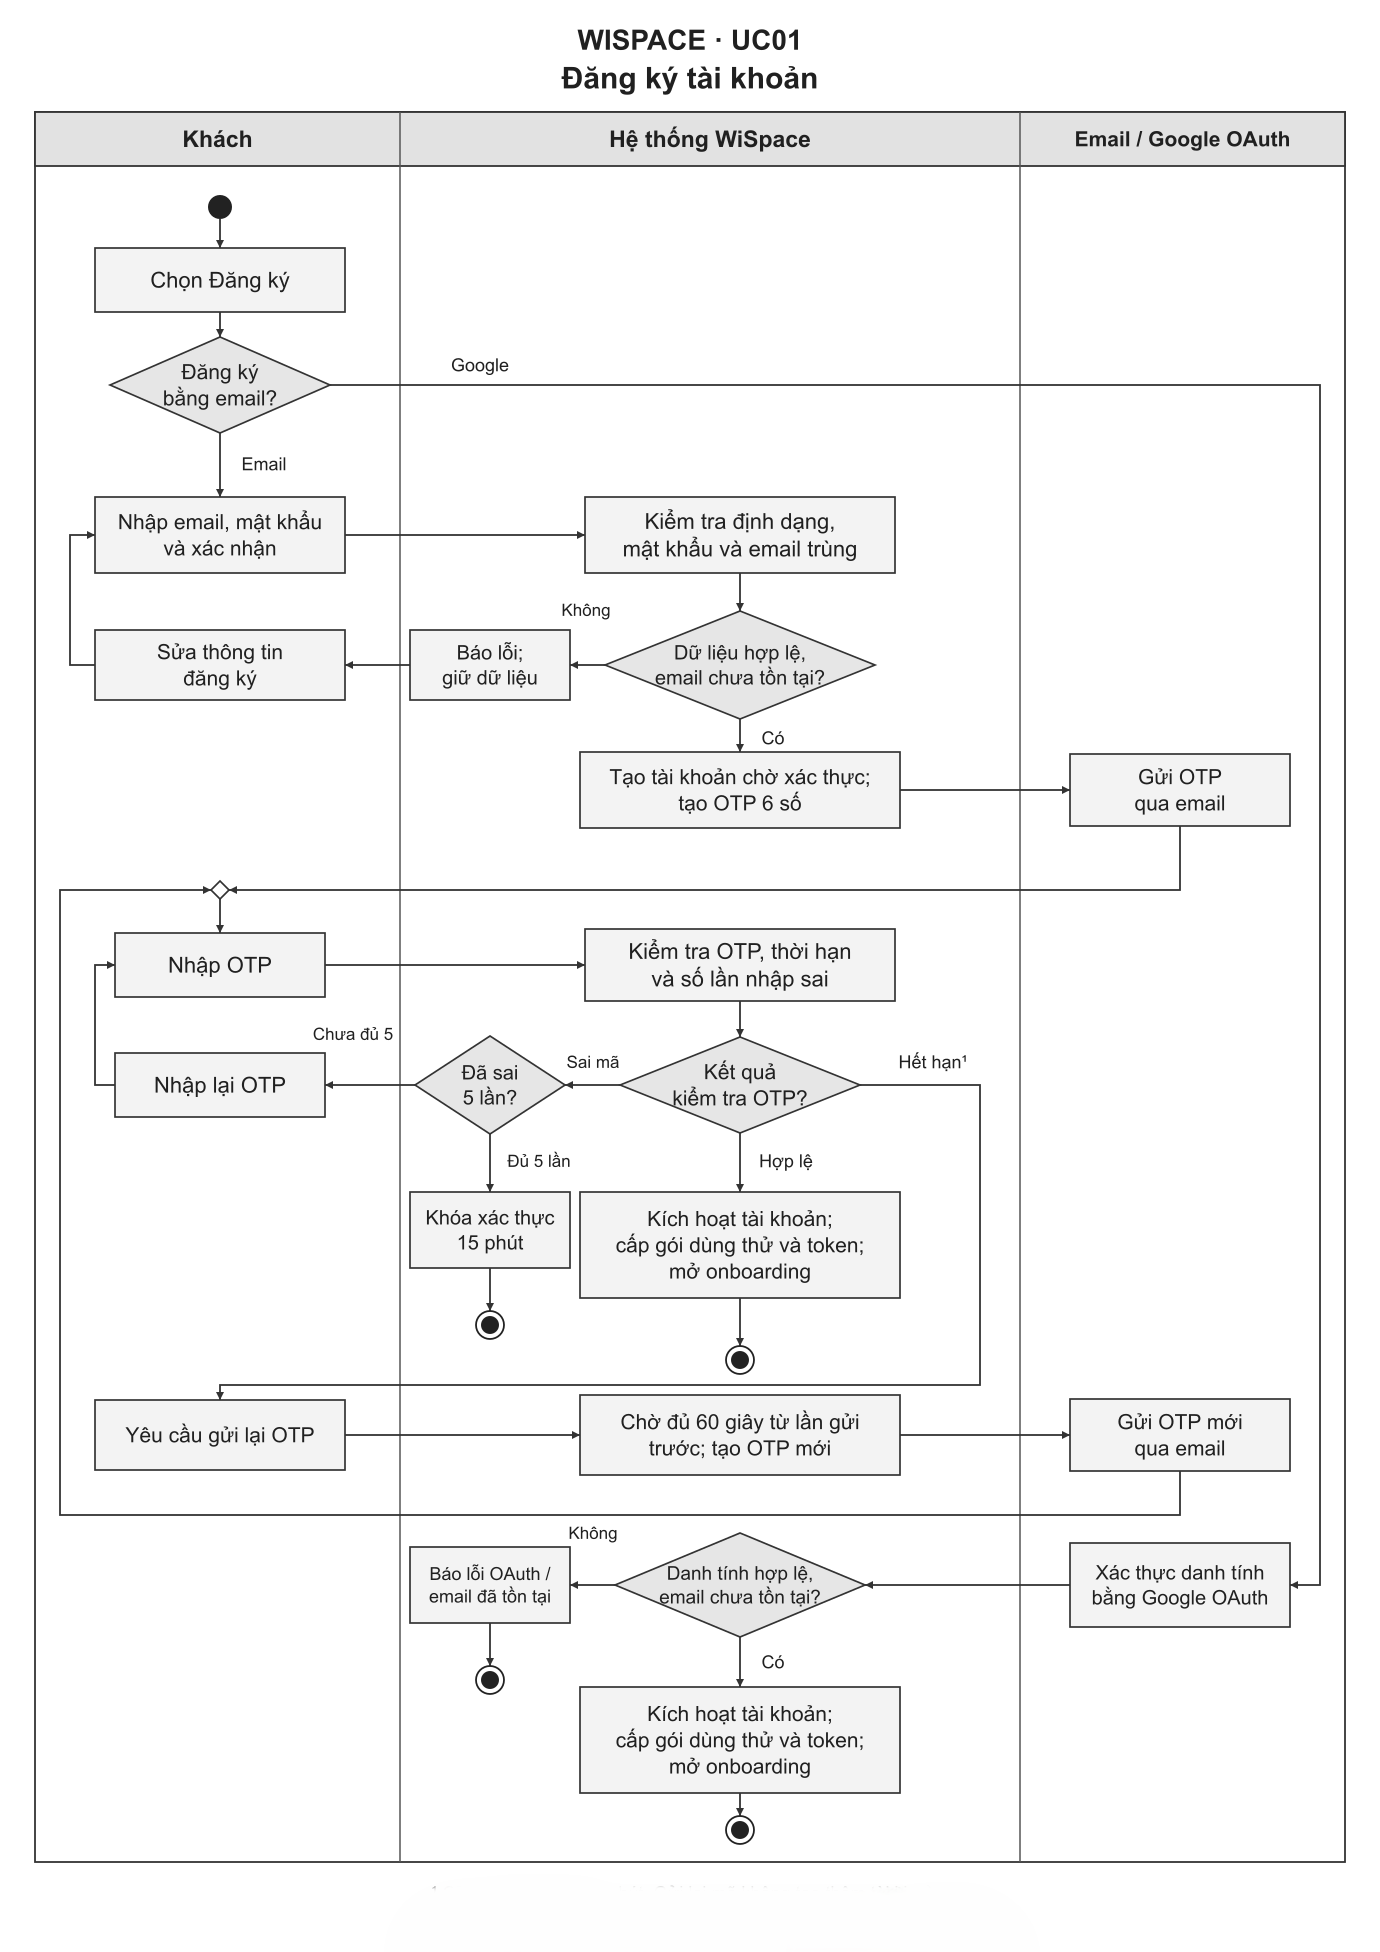
\includegraphics[width=\linewidth,height=0.72\textheight,keepaspectratio]{Images/Activity/Wispace/activity_uc01_register.png}
    \caption{Sơ đồ hoạt động Wispace -- Use-case 1: Đăng ký tài khoản}
    \label{wispace:fig:activity_uc01}
\end{figure}

Khách nhập thông tin đăng ký hoặc chọn Google. Xác thực thành công, hệ thống kích hoạt tài khoản và mở bước thiết lập ban đầu.
% activity-generated:end


\clearpage

\paragraph{Luồng hoạt động: Đăng nhập (Use-case 2)}

% activity-generated:start
\begin{figure}[H]
    \centering
    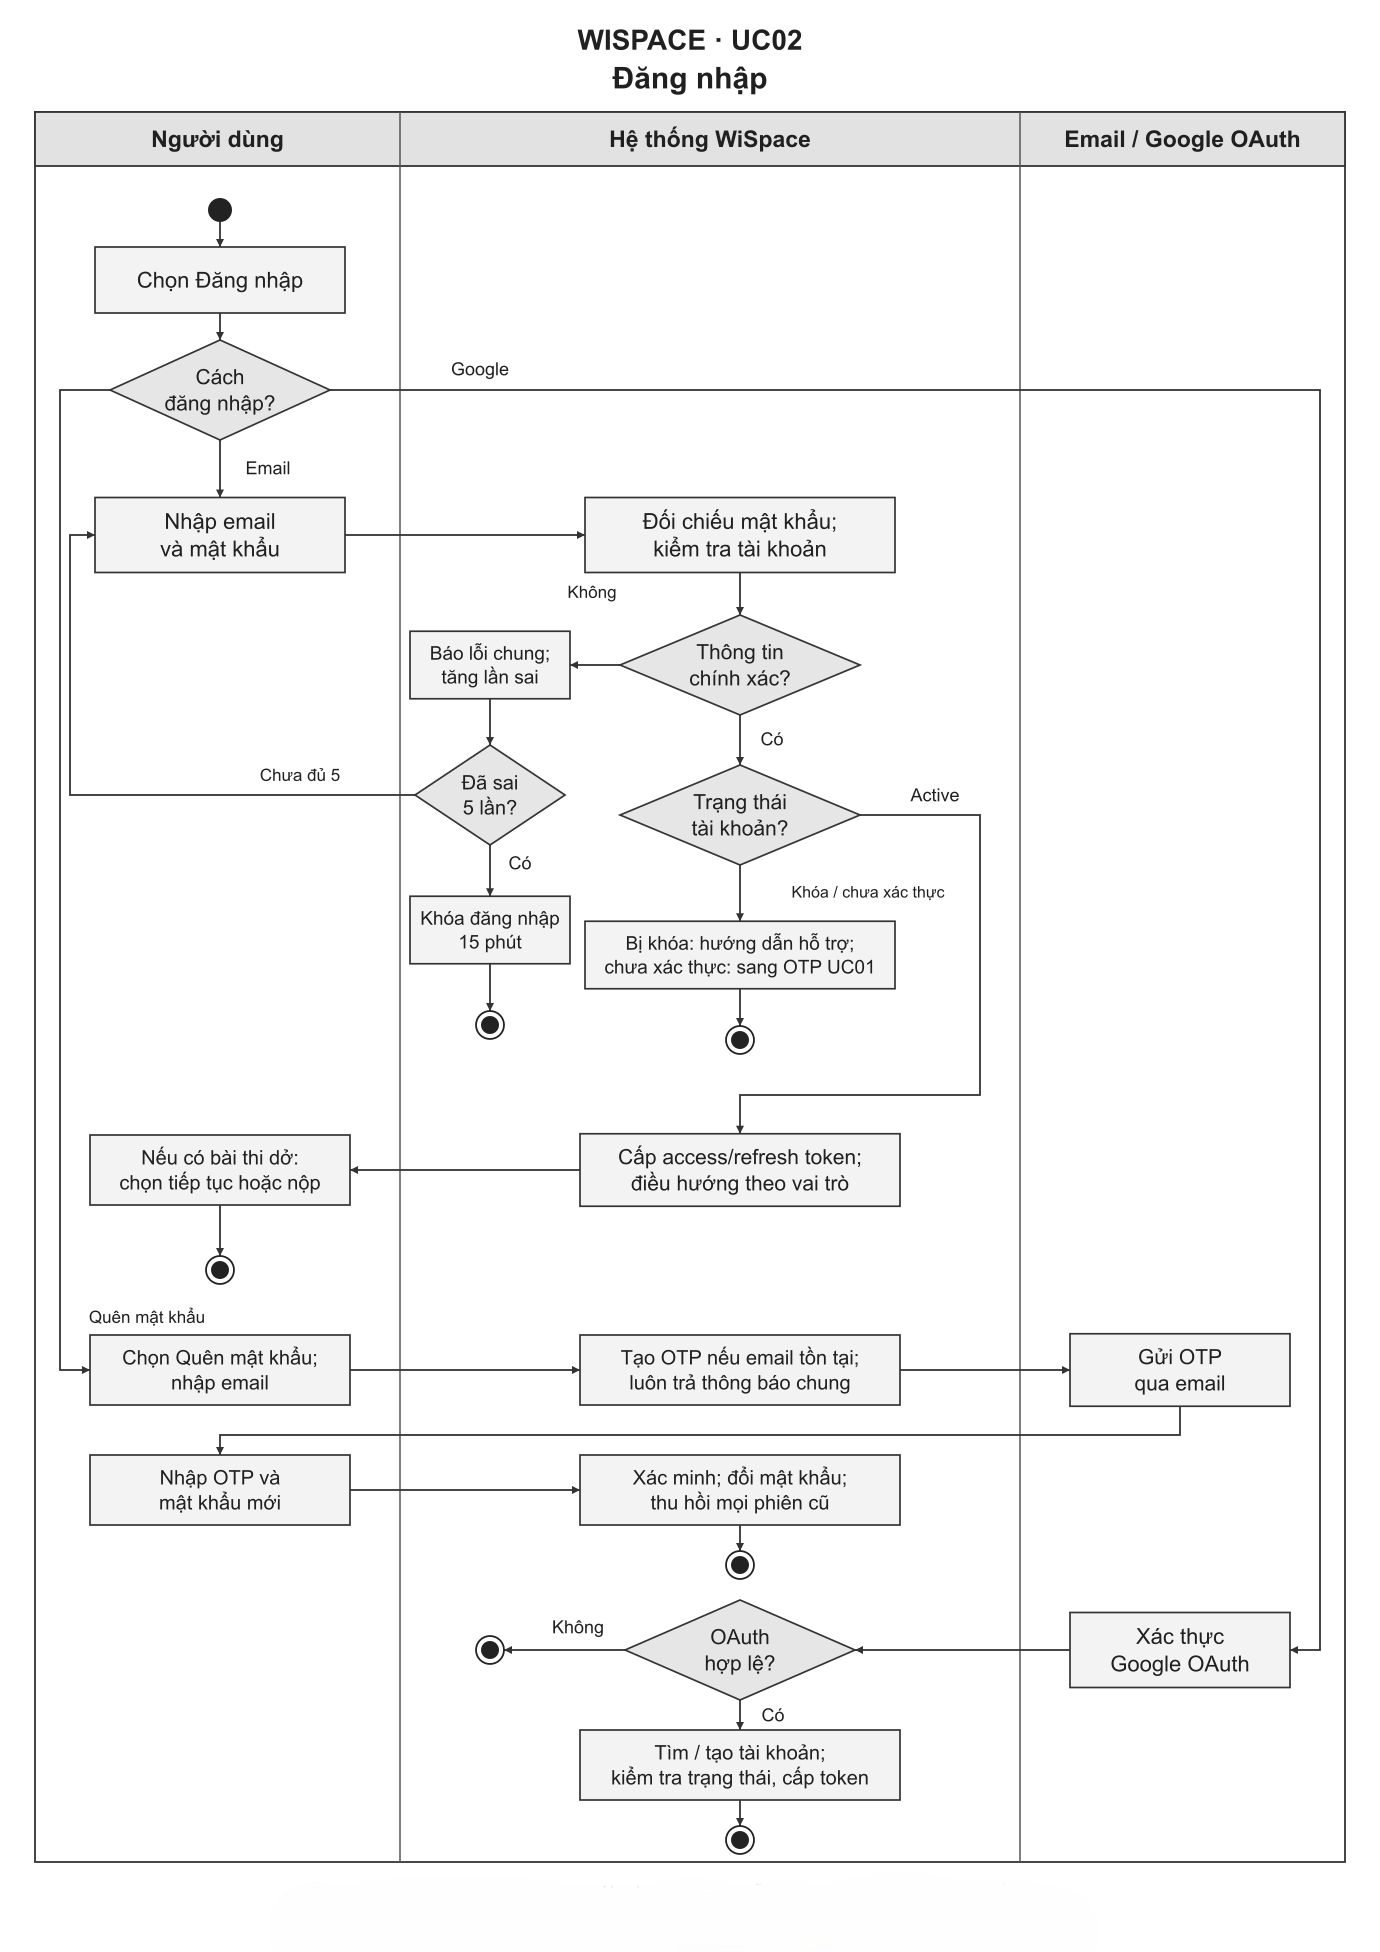
\includegraphics[width=\linewidth,height=0.72\textheight,keepaspectratio]{Images/Activity/Wispace/activity_uc02_login.png}
    \caption{Sơ đồ hoạt động Wispace -- Use-case 2: Đăng nhập}
    \label{wispace:fig:activity_uc02}
\end{figure}

Người dùng nhập thông tin đăng nhập hoặc chọn Google. Đăng nhập thành công, hệ thống chuyển đến giao diện phù hợp với vai trò.
% activity-generated:end


\clearpage

\paragraph{Luồng hoạt động: Đăng xuất (Use-case 3)}

% activity-generated:start
\begin{figure}[H]
    \centering
    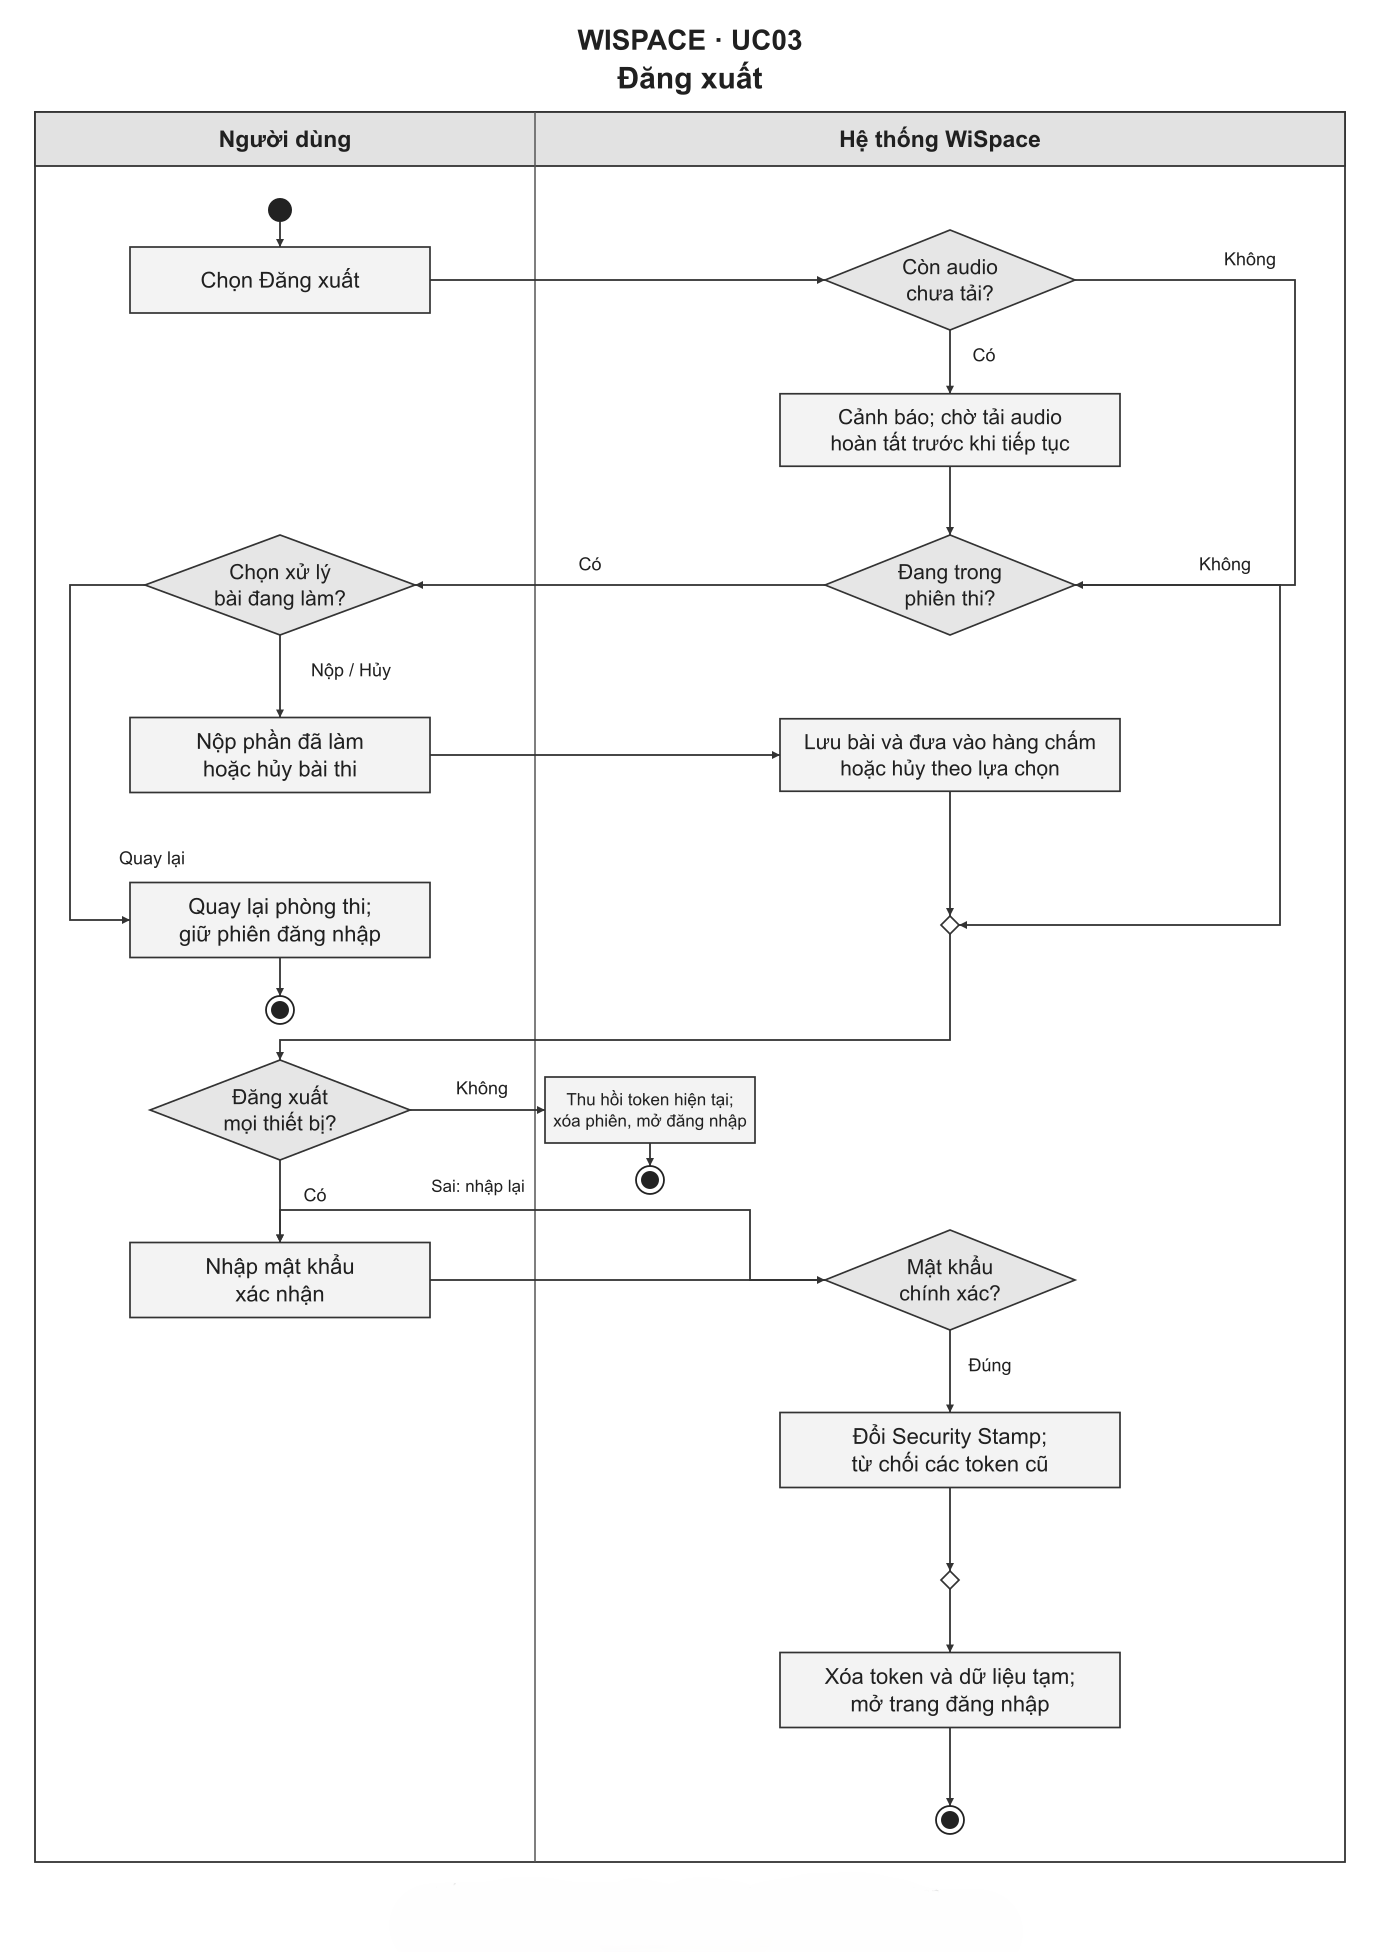
\includegraphics[width=\linewidth,height=0.72\textheight,keepaspectratio]{Images/Activity/Wispace/activity_uc03_logout.png}
    \caption{Sơ đồ hoạt động Wispace -- Use-case 3: Đăng xuất}
    \label{wispace:fig:activity_uc03}
\end{figure}

Người dùng chọn đăng xuất khỏi một hoặc tất cả thiết bị. Giao diện trở về trang đăng nhập.
% activity-generated:end


\clearpage

\paragraph{Luồng hoạt động: Quản lý hồ sơ cá nhân (Use-case 4)}

% activity-generated:start
\begin{figure}[H]
    \centering
    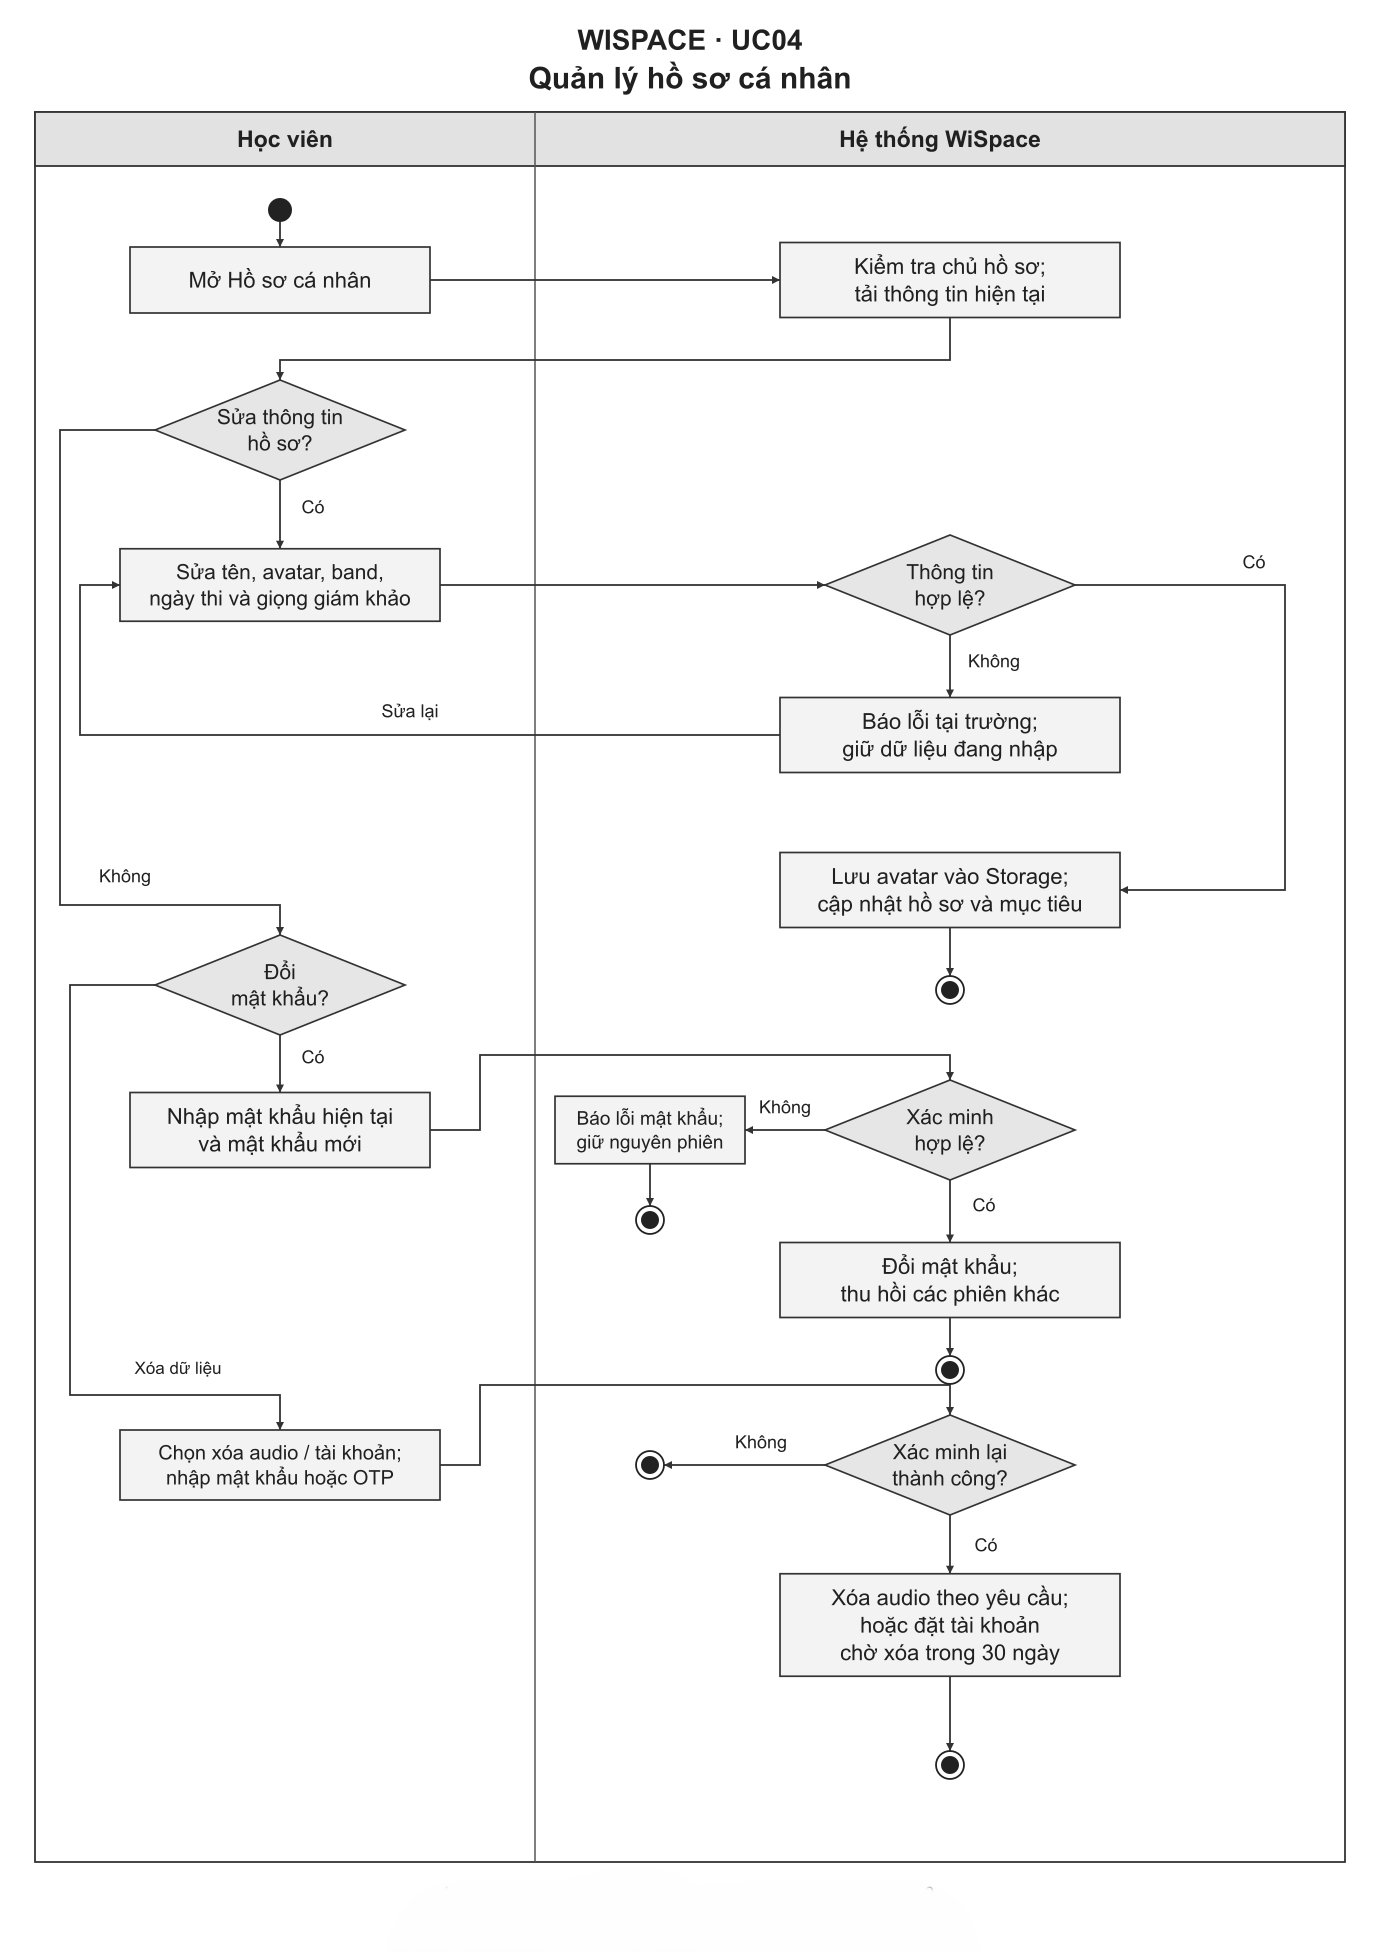
\includegraphics[width=\linewidth,height=0.72\textheight,keepaspectratio]{Images/Activity/Wispace/activity_uc04_profile.png}
    \caption{Sơ đồ hoạt động Wispace -- Use-case 4: Quản lý hồ sơ cá nhân}
    \label{wispace:fig:activity_uc04}
\end{figure}

Học viên mở hồ sơ và chọn nội dung cần thay đổi. Hệ thống xác nhận kết quả cập nhật hoặc xử lý yêu cầu xóa dữ liệu.
% activity-generated:end


\clearpage

\paragraph{Luồng hoạt động: Quản lý người dùng (Use-case 5)}

% activity-generated:start
\begin{figure}[H]
    \centering
    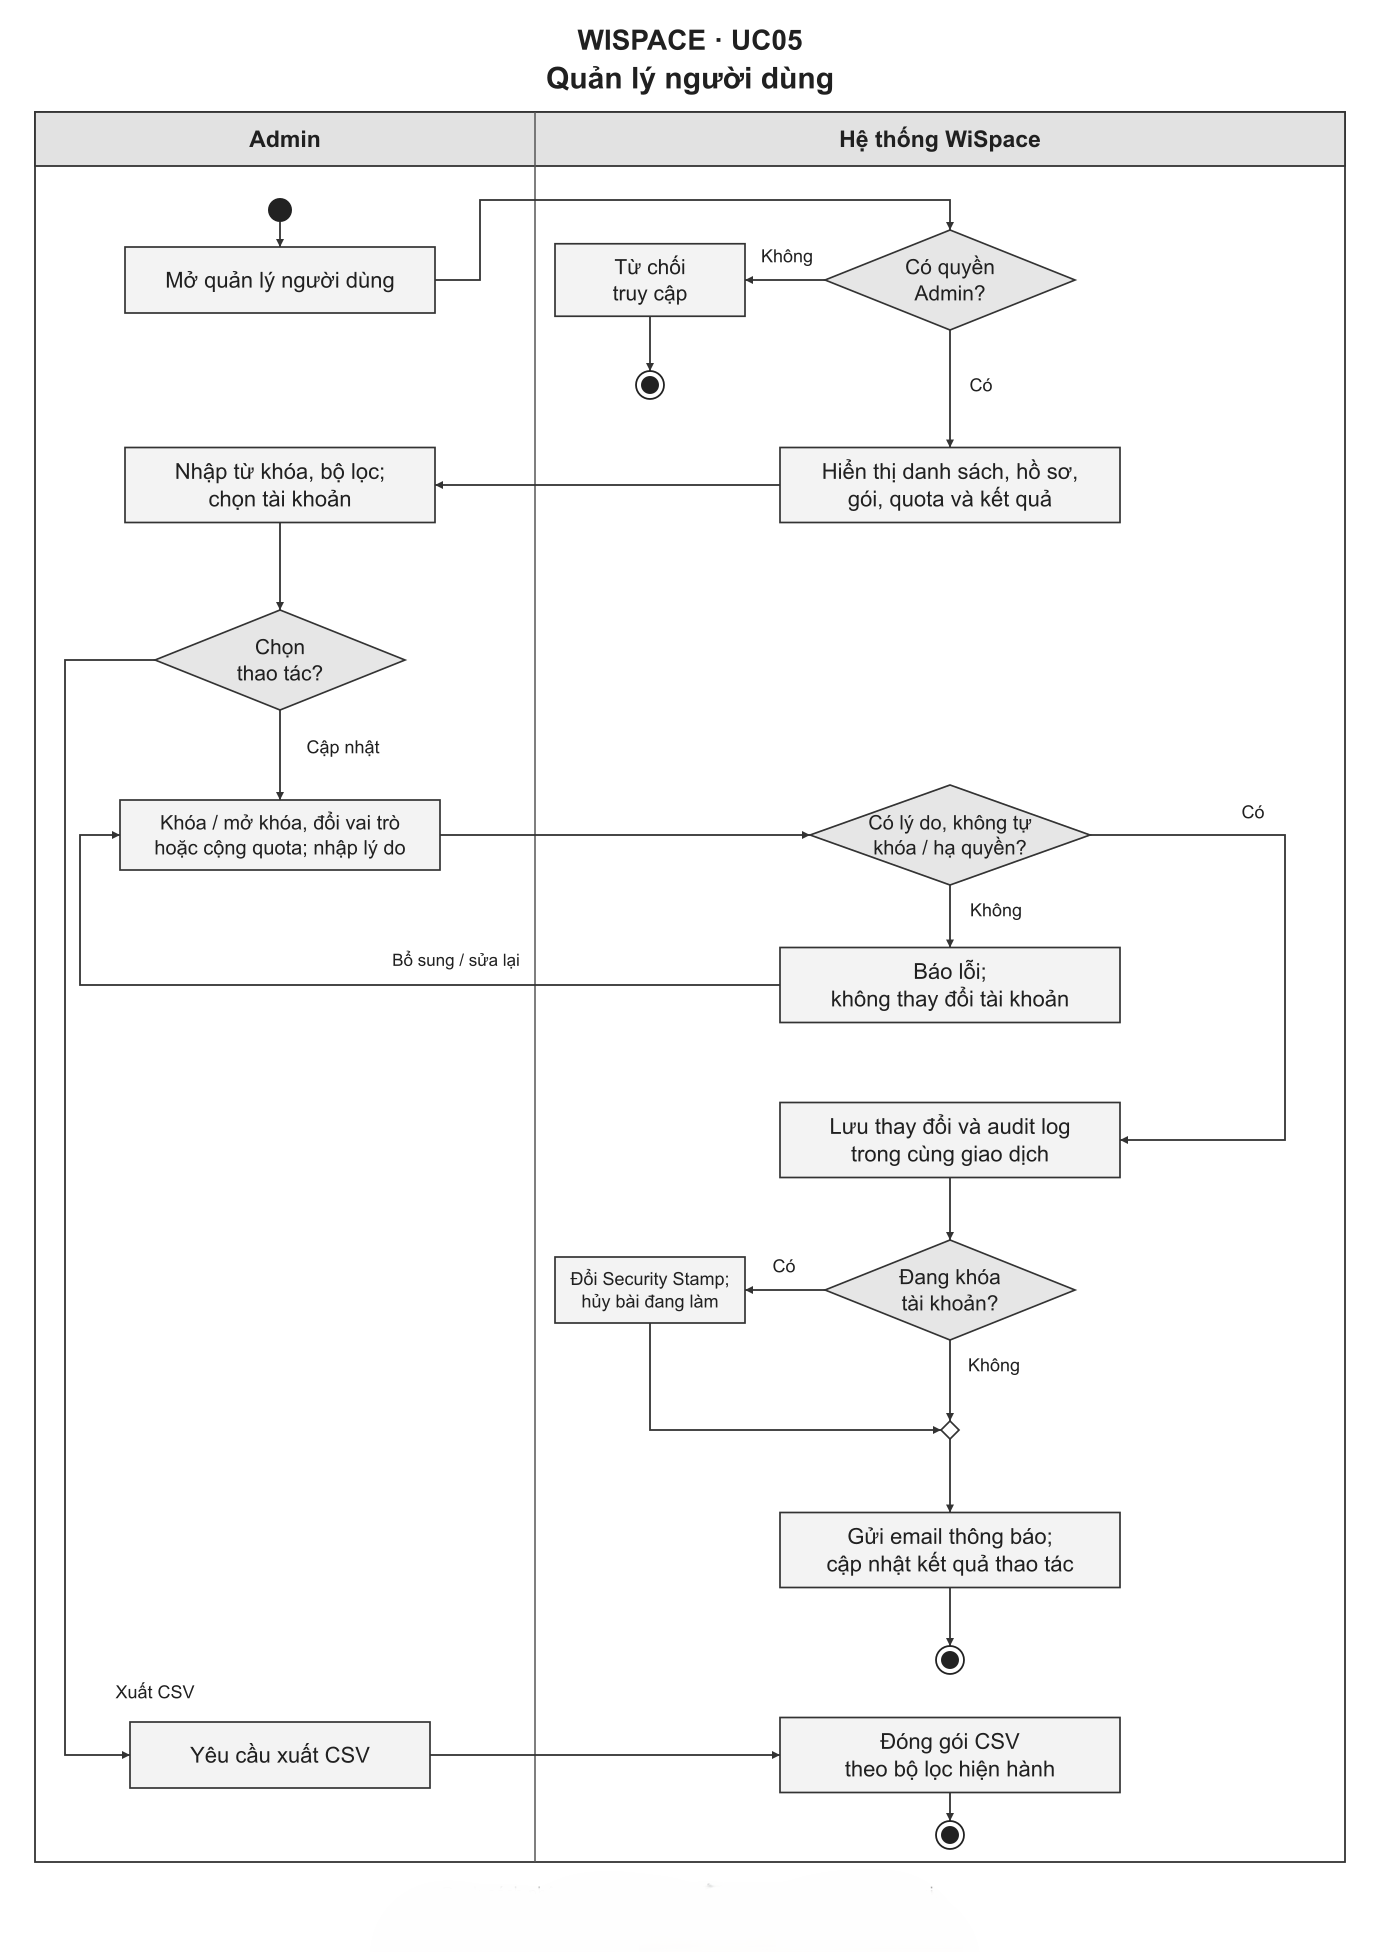
\includegraphics[width=\linewidth,height=0.72\textheight,keepaspectratio]{Images/Activity/Wispace/activity_uc05_user_management.png}
    \caption{Sơ đồ hoạt động Wispace -- Use-case 5: Quản lý người dùng}
    \label{wispace:fig:activity_uc05}
\end{figure}

Admin tìm kiếm và chọn người dùng cần quản lý. Thay đổi được lưu kèm nhật ký; Admin nhận kết quả hoặc xuất danh sách.
% activity-generated:end


\clearpage

\paragraph{Luồng hoạt động: Xem và tìm kiếm đề thi (Use-case 6)}

% activity-generated:start
\begin{figure}[H]
    \centering
    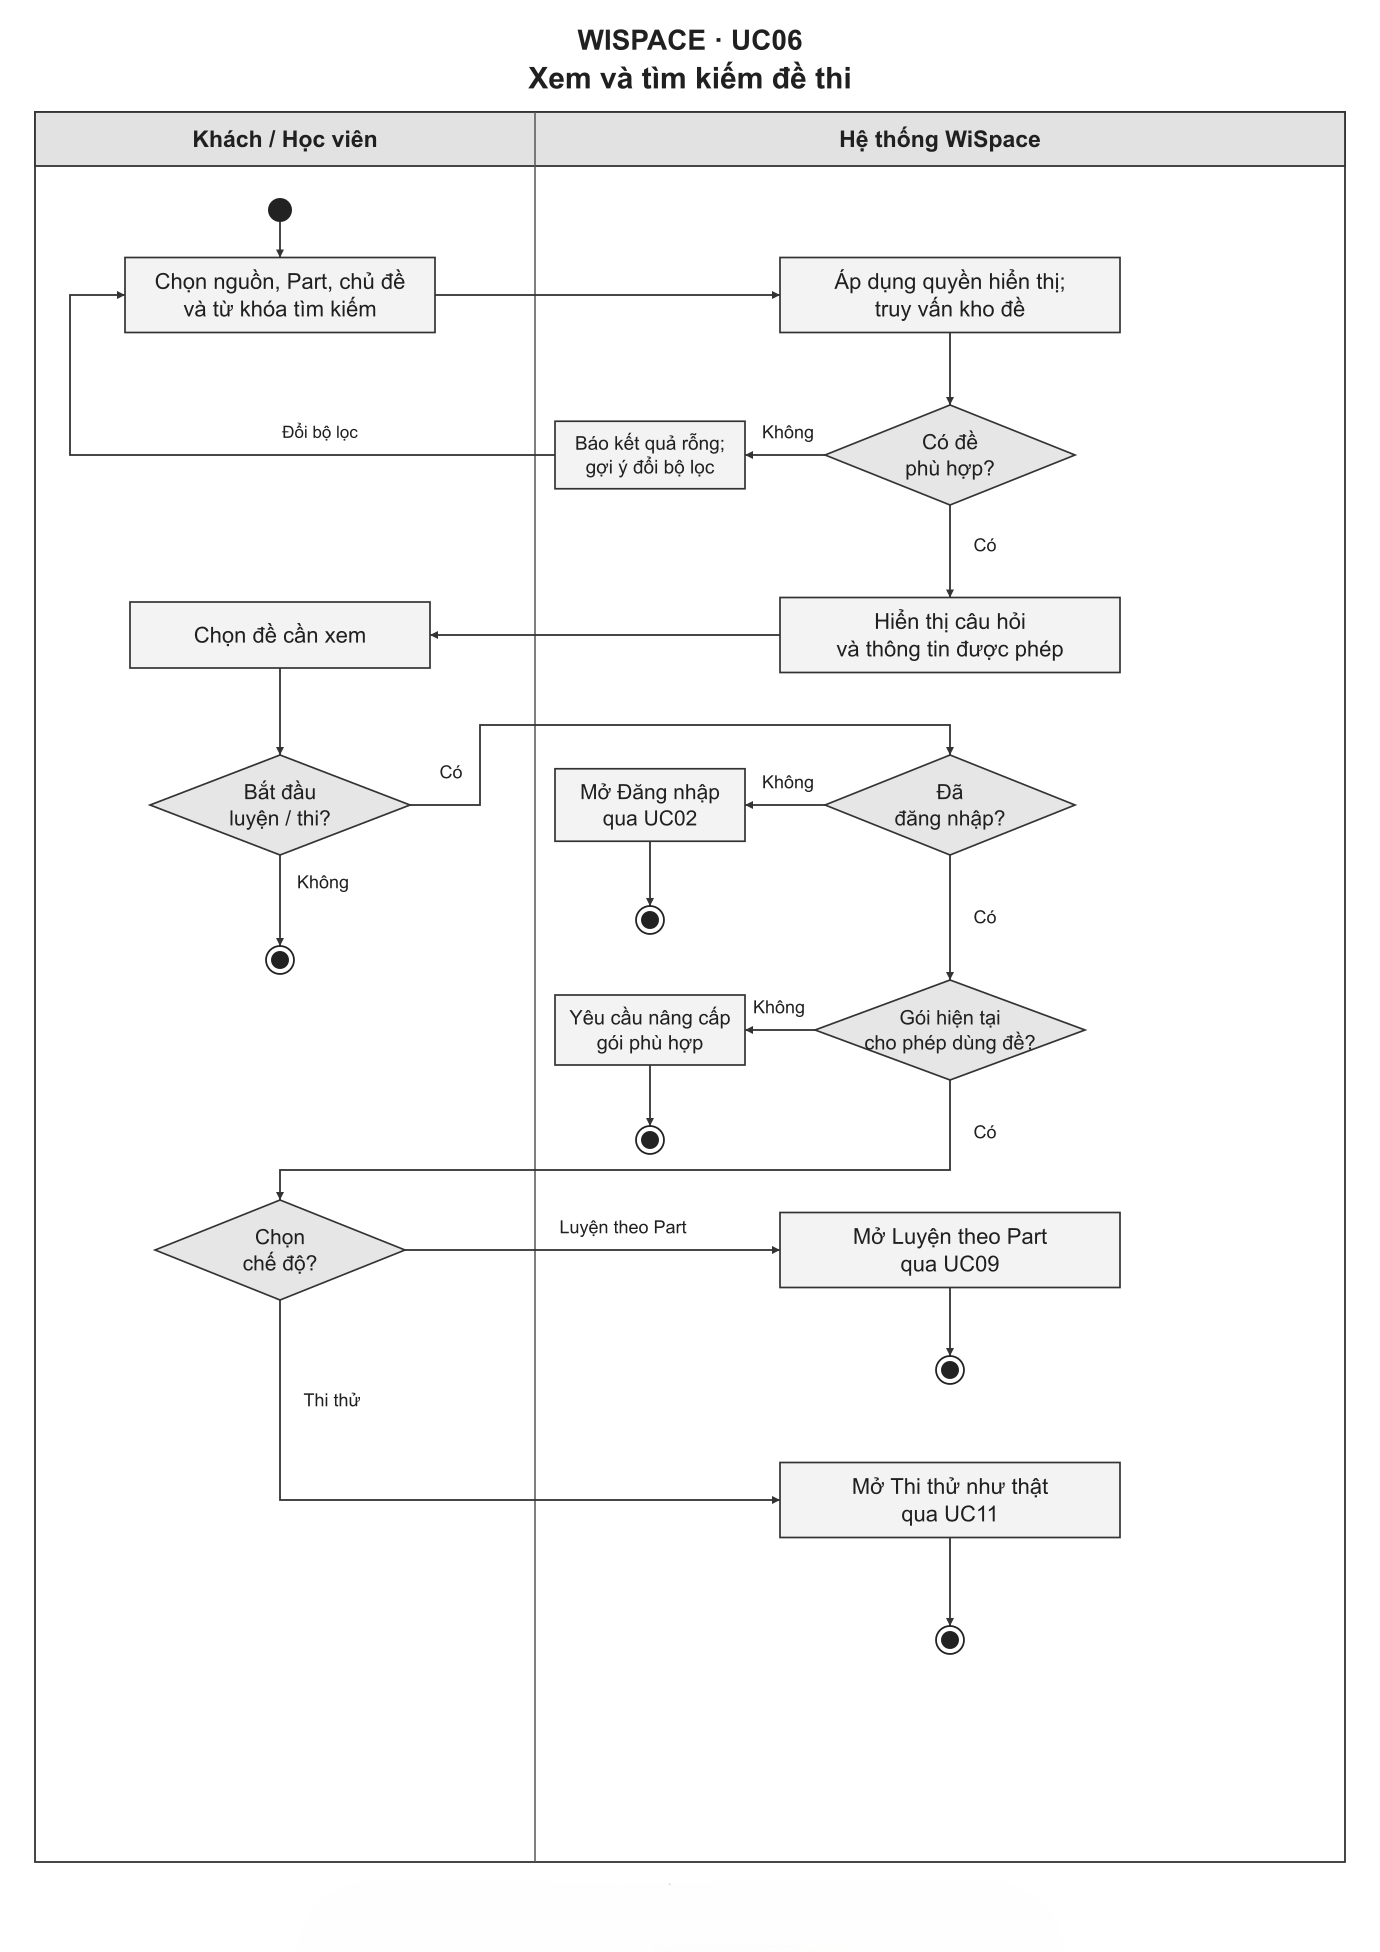
\includegraphics[width=\linewidth,height=0.72\textheight,keepaspectratio]{Images/Activity/Wispace/activity_uc06_browse_tests.png}
    \caption{Sơ đồ hoạt động Wispace -- Use-case 6: Xem và tìm kiếm đề thi}
    \label{wispace:fig:activity_uc06}
\end{figure}

Người dùng chọn nguồn đề, Part, chủ đề hoặc từ khóa. Hệ thống kiểm tra đăng nhập, quyền sử dụng và mở chức năng tương ứng.
% activity-generated:end


\clearpage

\paragraph{Luồng hoạt động: Thêm đề thi (Use-case 7)}

% activity-generated:start
\begin{figure}[H]
    \centering
    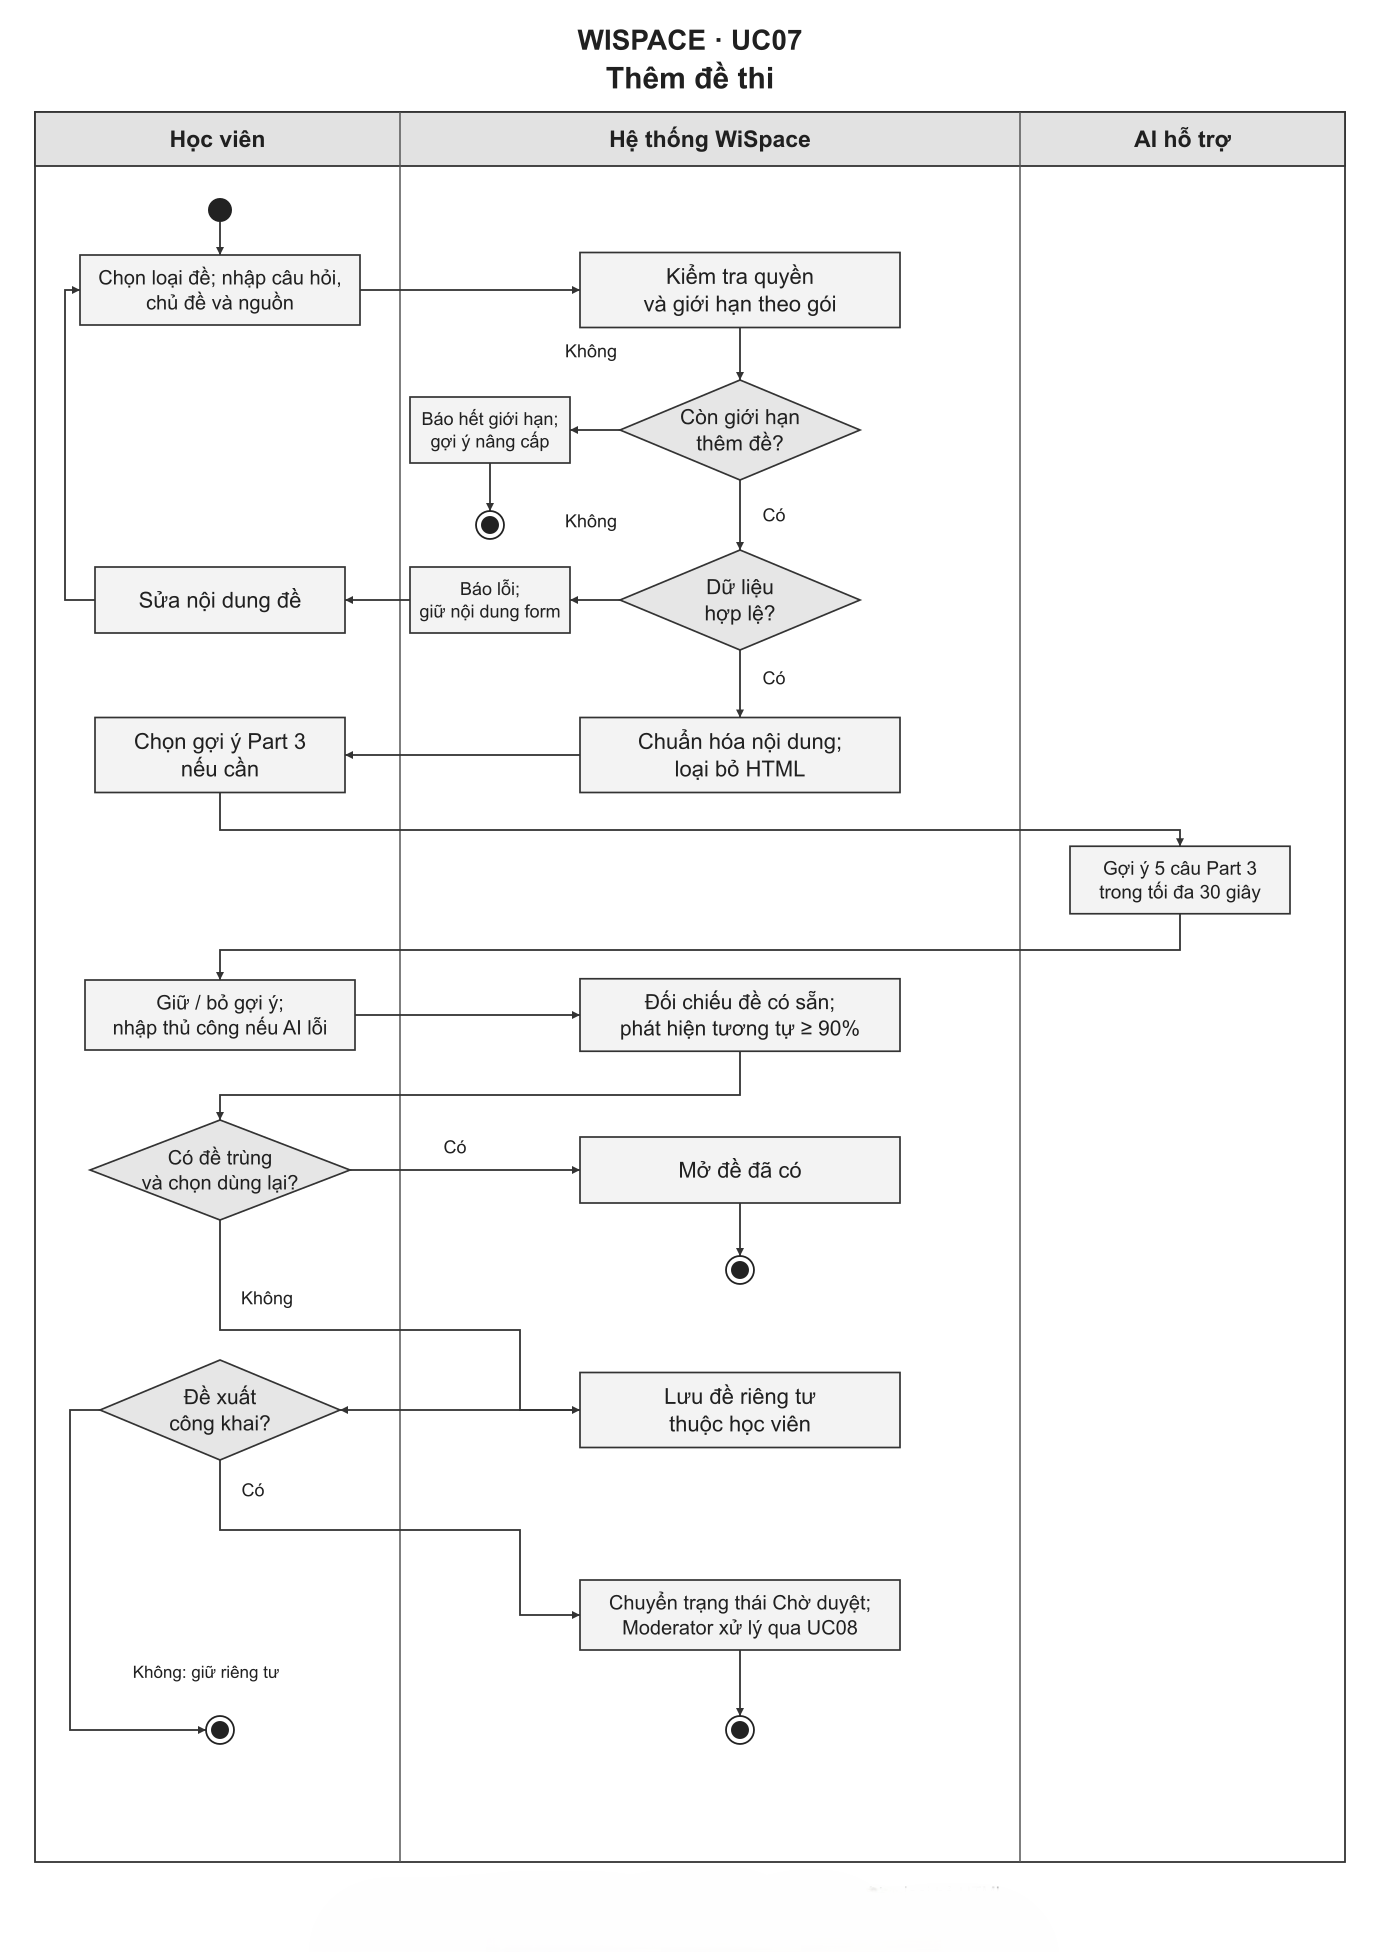
\includegraphics[width=\linewidth,height=0.72\textheight,keepaspectratio]{Images/Activity/Wispace/activity_uc07_add_test.png}
    \caption{Sơ đồ hoạt động Wispace -- Use-case 7: Thêm đề thi}
    \label{wispace:fig:activity_uc07}
\end{figure}

Học viên nhập câu hỏi và thông tin đề cần tạo. Nếu đề xuất công khai, đề được chuyển sang hàng chờ kiểm duyệt.
% activity-generated:end


\clearpage

\paragraph{Luồng hoạt động: Quản lý và duyệt kho đề (Use-case 8)}

% activity-generated:start
\begin{figure}[H]
    \centering
    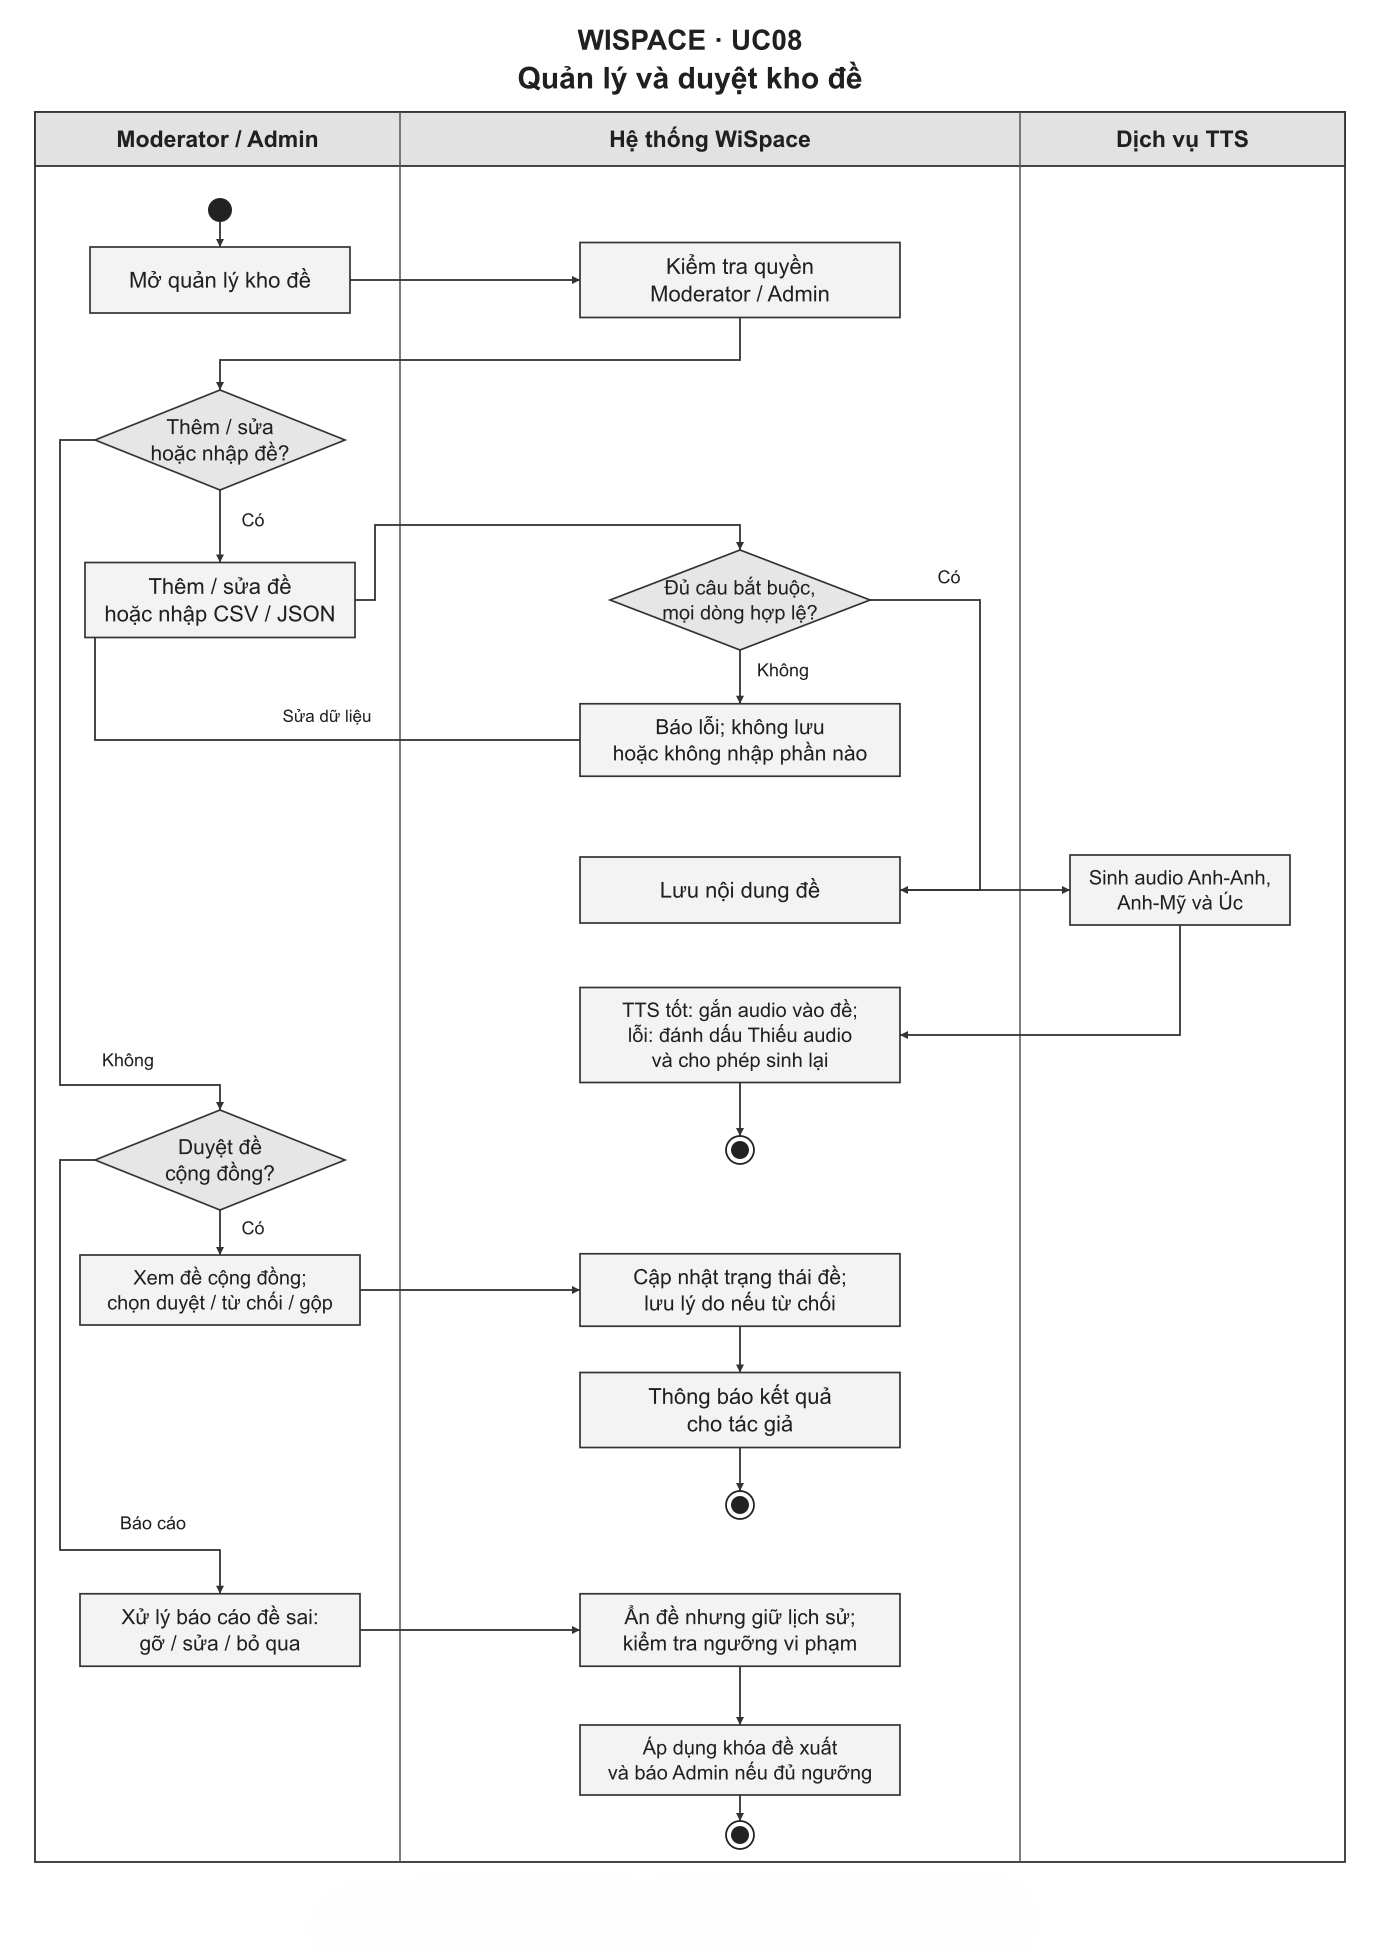
\includegraphics[width=\linewidth,height=0.72\textheight,keepaspectratio]{Images/Activity/Wispace/activity_uc08_moderate_tests.png}
    \caption{Sơ đồ hoạt động Wispace -- Use-case 8: Quản lý và duyệt kho đề}
    \label{wispace:fig:activity_uc08}
\end{figure}

Moderator hoặc Admin chọn thêm, sửa, nhập đề hoặc duyệt đề cộng đồng. Các báo cáo đề sai được xử lý mà vẫn giữ lịch sử bài làm.
% activity-generated:end


\clearpage

\paragraph{Luồng hoạt động: Luyện tập theo Part (Use-case 9)}

% activity-generated:start
\begin{figure}[H]
    \centering
    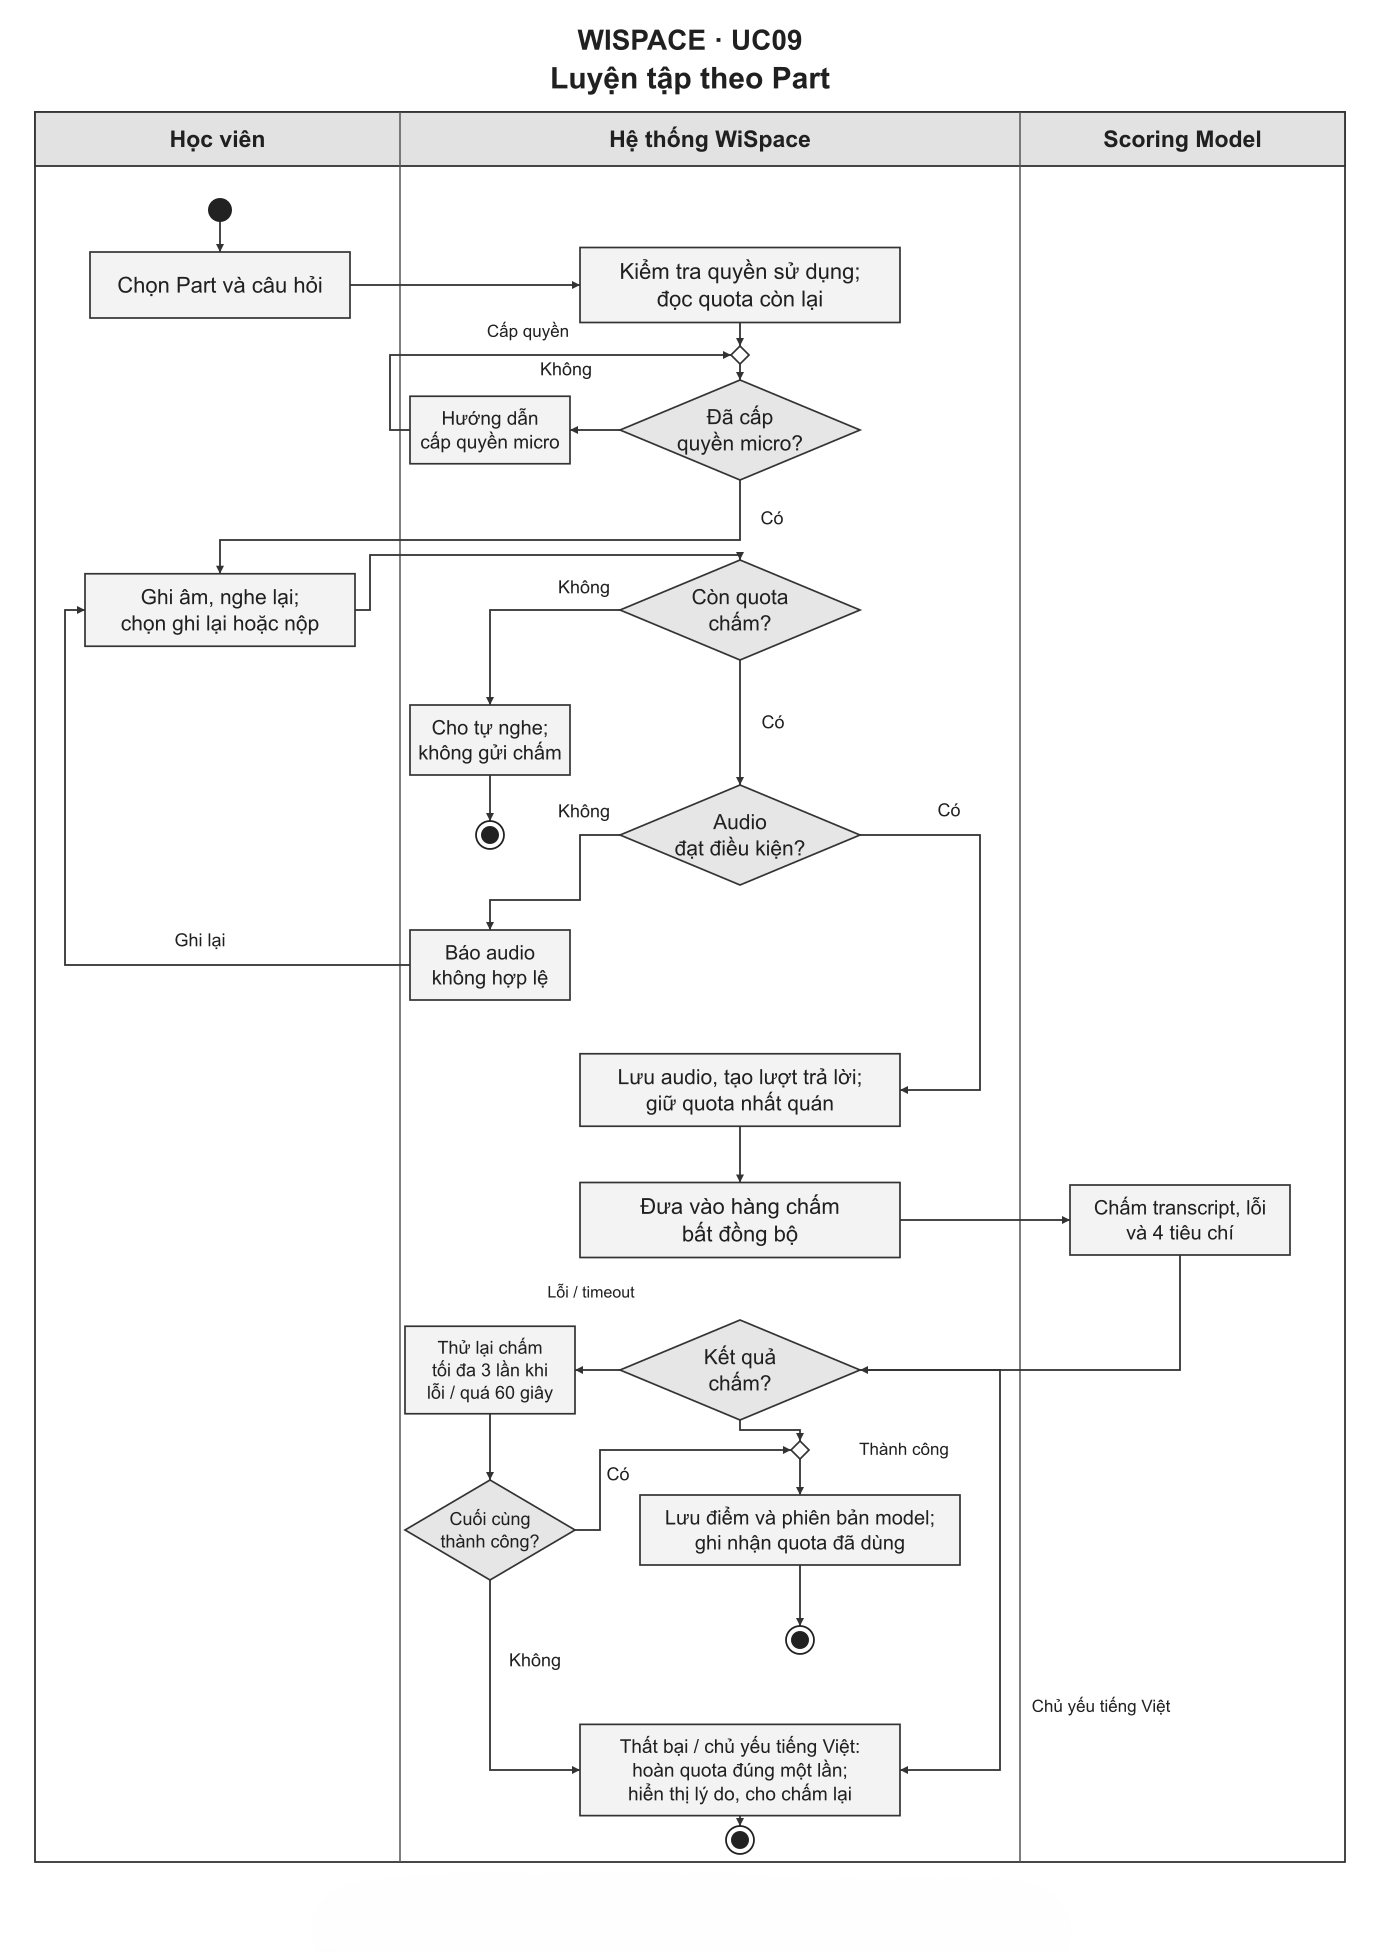
\includegraphics[width=\linewidth,height=0.72\textheight,keepaspectratio]{Images/Activity/Wispace/activity_uc09_part_practice.png}
    \caption{Sơ đồ hoạt động Wispace -- Use-case 9: Luyện tập theo Part}
    \label{wispace:fig:activity_uc09}
\end{figure}

Học viên chọn câu hỏi, ghi âm và nộp câu trả lời. Hệ thống lưu kết quả; nếu chấm thất bại cuối cùng thì hoàn hạn mức.
% activity-generated:end


\clearpage

\paragraph{Luồng hoạt động: Xem kết quả và luyện lại (Use-case 10)}

% activity-generated:start
\begin{figure}[H]
    \centering
    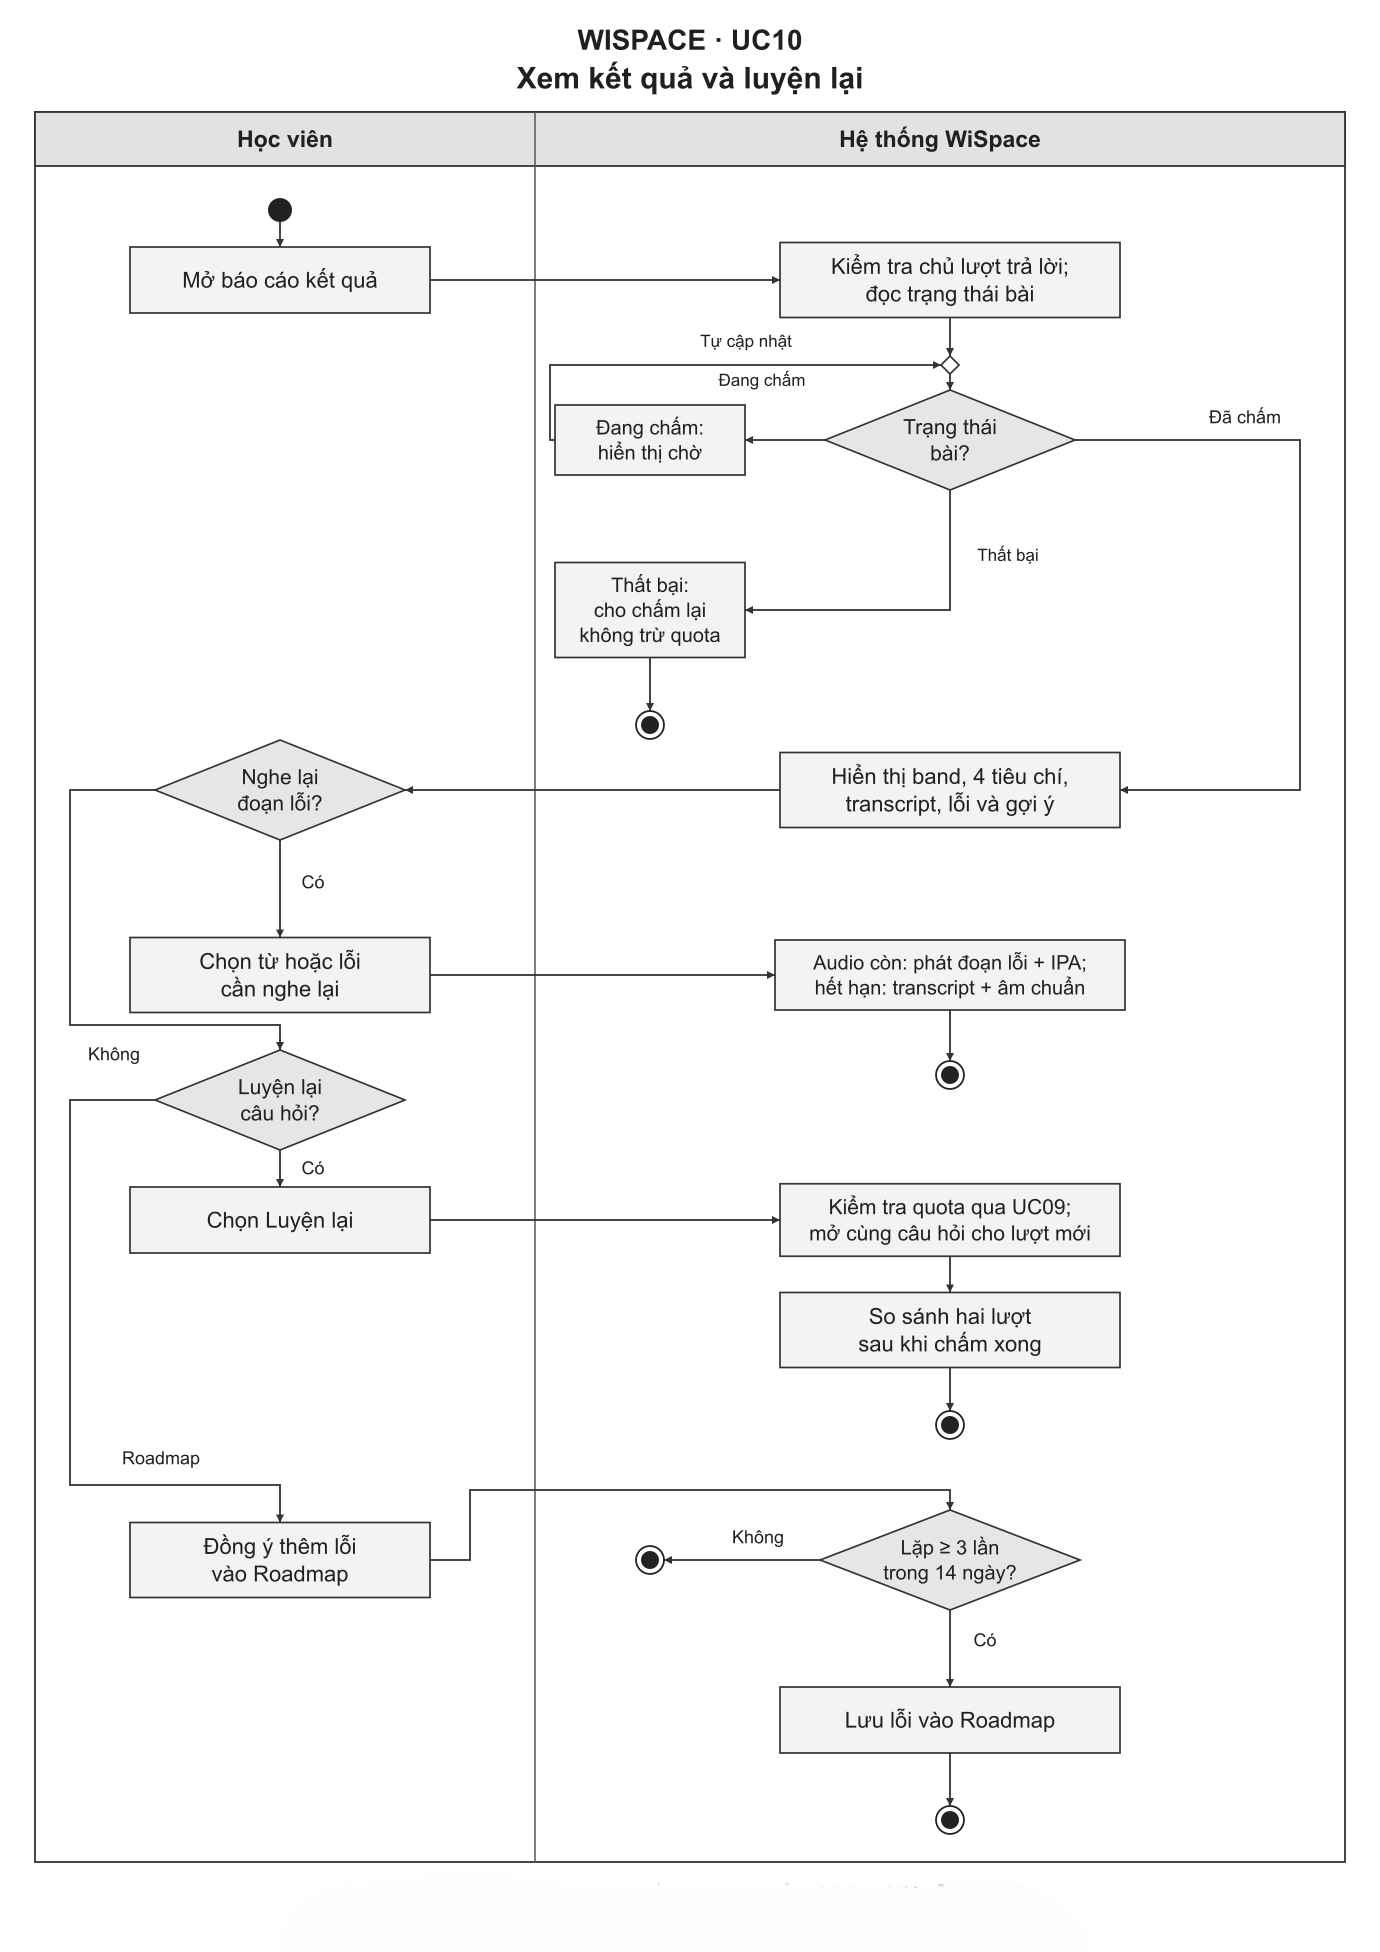
\includegraphics[width=\linewidth,height=0.72\textheight,keepaspectratio]{Images/Activity/Wispace/activity_uc10_results_retry.png}
    \caption{Sơ đồ hoạt động Wispace -- Use-case 10: Xem kết quả và luyện lại}
    \label{wispace:fig:activity_uc10}
\end{figure}

Học viên mở kết quả của bài đã nộp. Hệ thống thực hiện lựa chọn và lưu kết quả liên quan.
% activity-generated:end


\clearpage

\paragraph{Luồng hoạt động: Thi thử như thật (Use-case 11)}

% activity-generated:start
\begin{figure}[H]
    \centering
    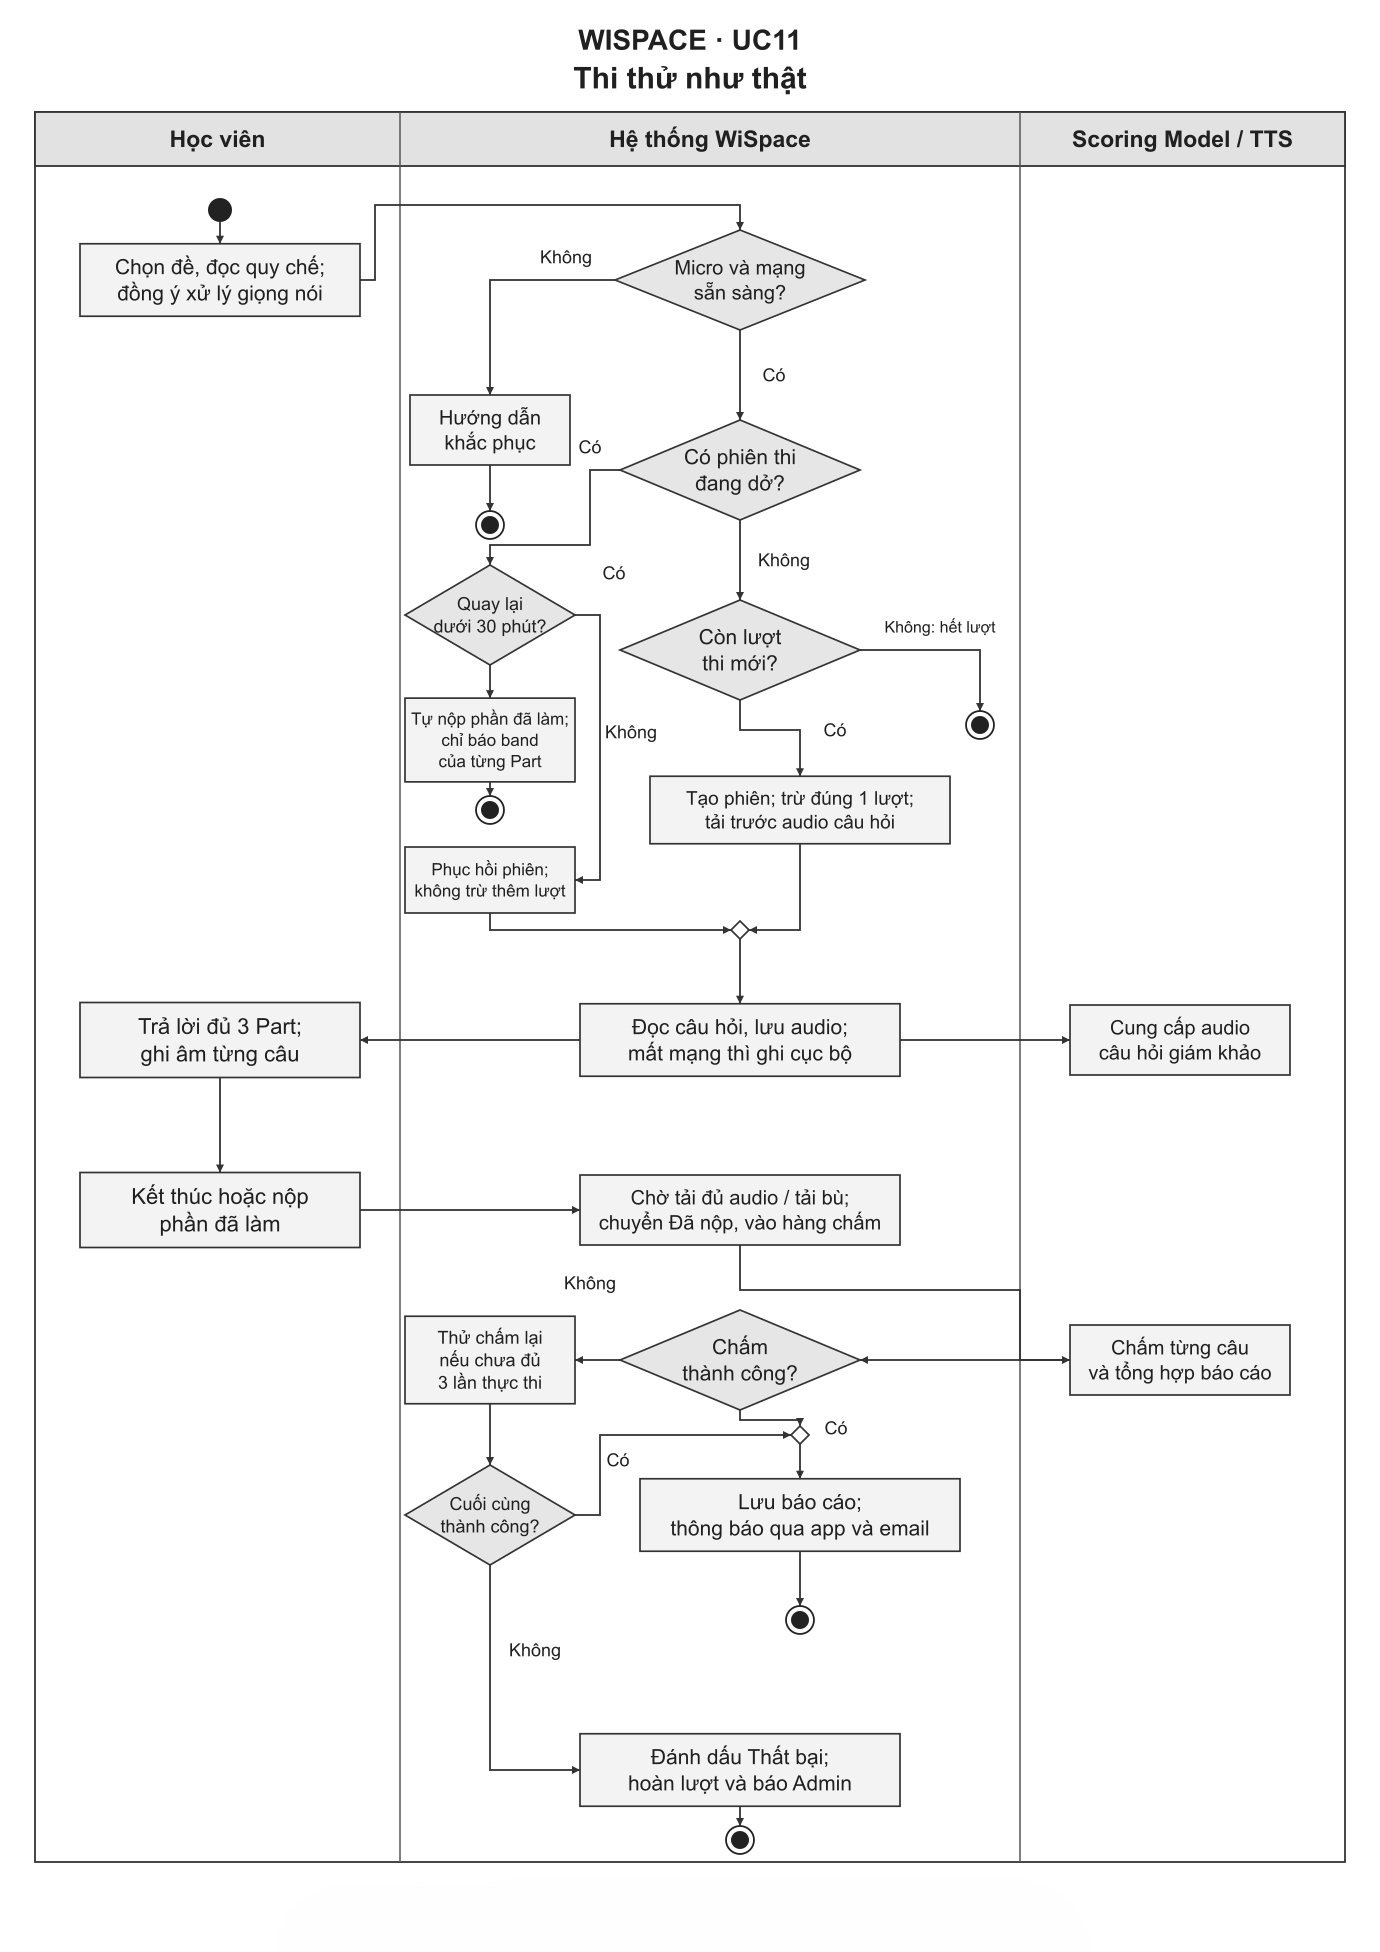
\includegraphics[width=\linewidth,height=0.72\textheight,keepaspectratio]{Images/Activity/Wispace/activity_uc11_mock_test.png}
    \caption{Sơ đồ hoạt động Wispace -- Use-case 11: Thi thử như thật}
    \label{wispace:fig:activity_uc11}
\end{figure}

Học viên chọn đề, kiểm tra thiết bị và bắt đầu hoặc tiếp tục phiên thi. Báo cáo được lưu và thông báo; nếu chấm thất bại cuối cùng thì hoàn lượt.
% activity-generated:end


\clearpage

\paragraph{Luồng hoạt động: Xem lịch sử và tiến bộ (Use-case 12)}

% activity-generated:start
\begin{figure}[H]
    \centering
    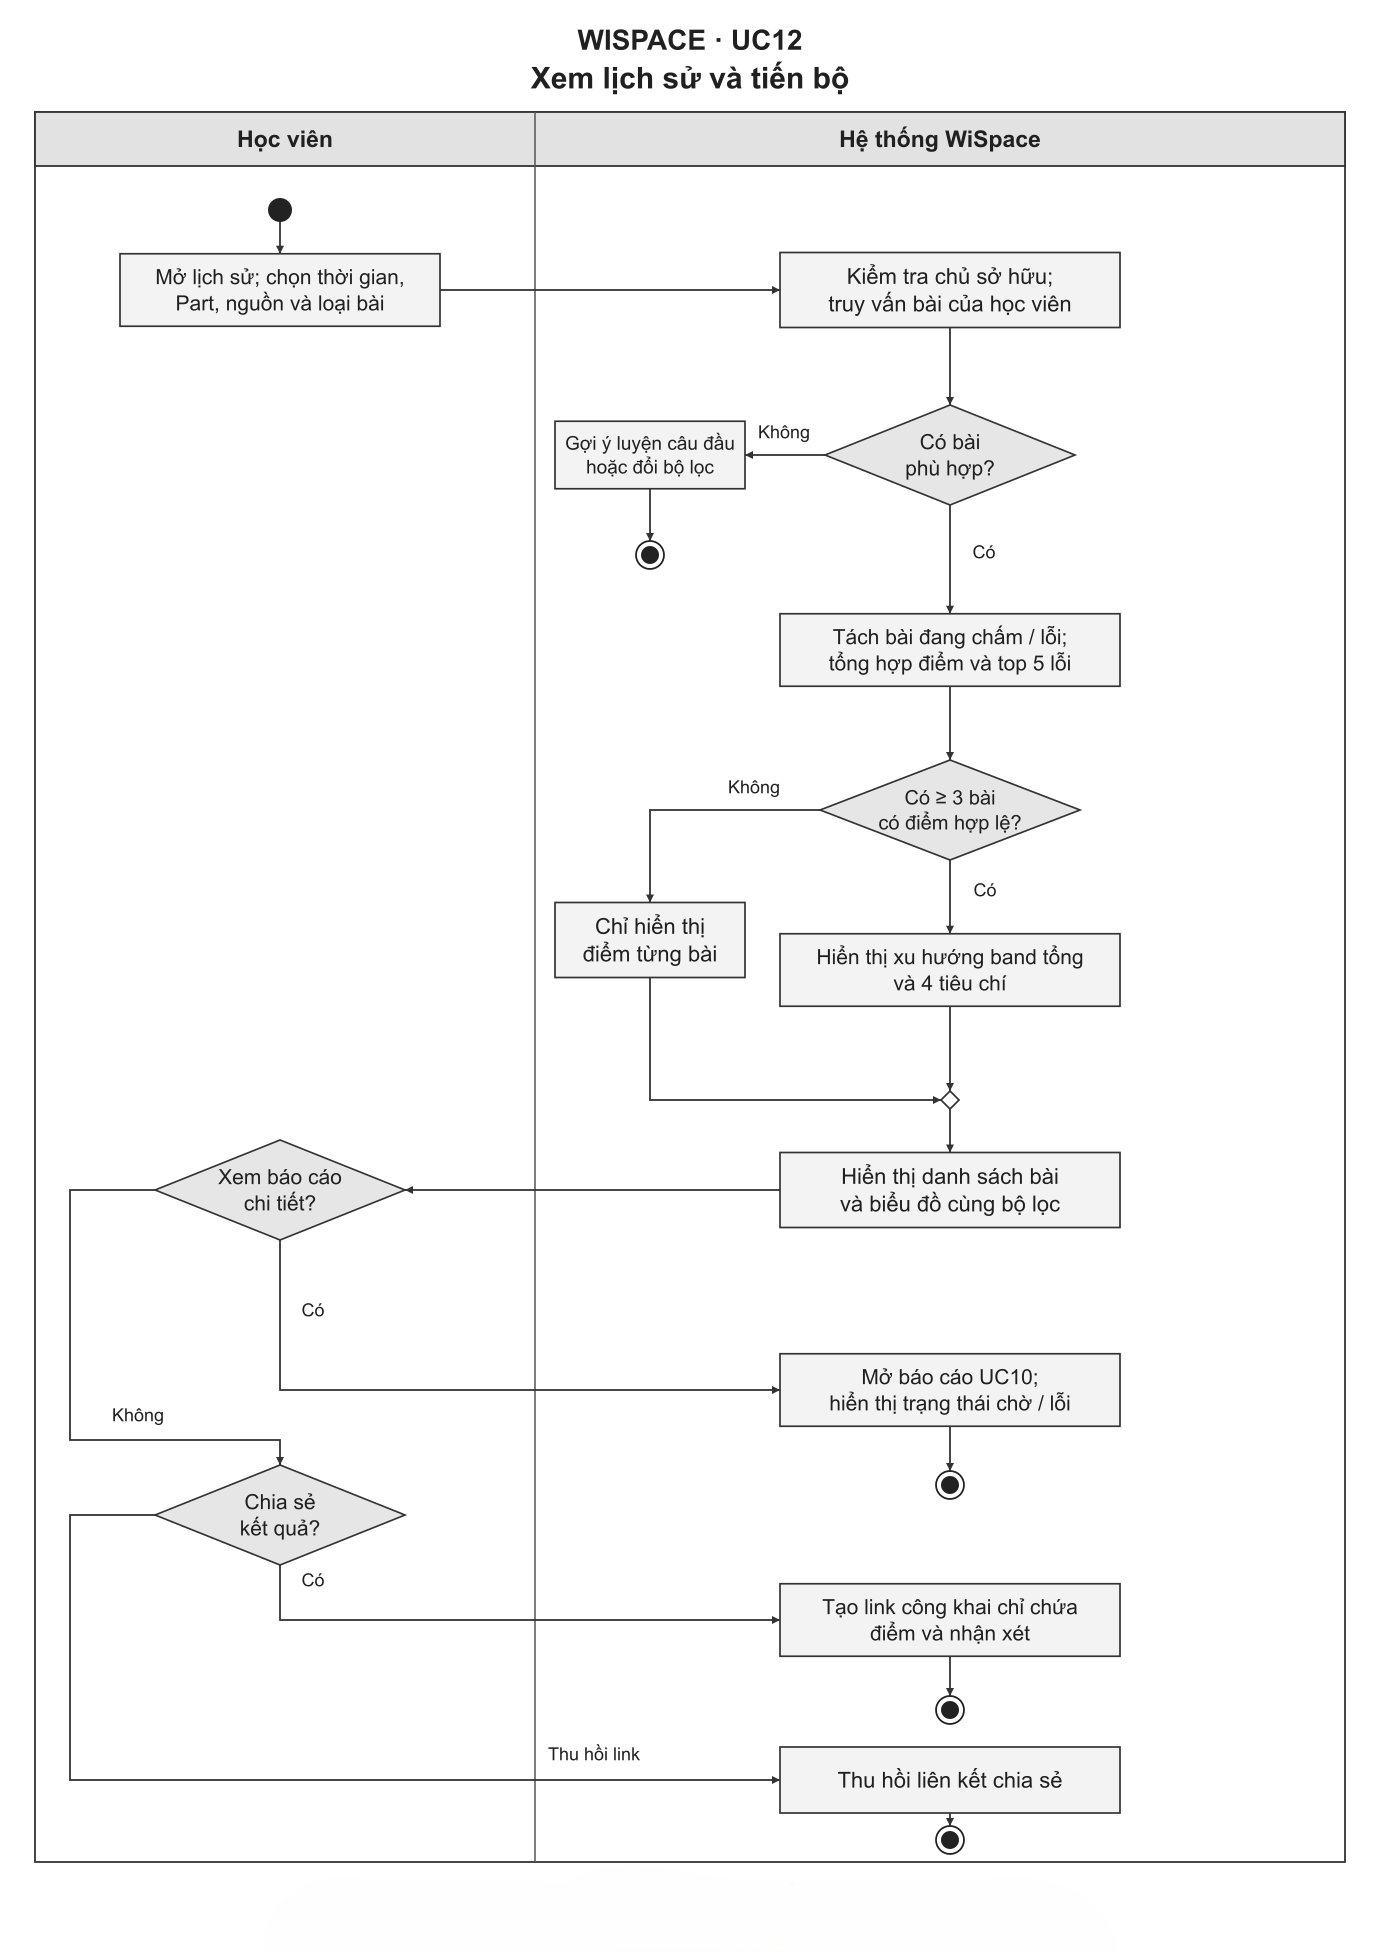
\includegraphics[width=\linewidth,height=0.72\textheight,keepaspectratio]{Images/Activity/Wispace/activity_uc12_progress_history.png}
    \caption{Sơ đồ hoạt động Wispace -- Use-case 12: Xem lịch sử và tiến bộ}
    \label{wispace:fig:activity_uc12}
\end{figure}

Học viên mở lịch sử và chọn bộ lọc. Hệ thống mở báo cáo, tạo hoặc thu hồi liên kết theo lựa chọn.
% activity-generated:end


\clearpage
\subsubsection{Sơ đồ luồng dữ liệu DFD}
\label{wispace:sec:dfd}

Phần này trình bày sơ đồ ngữ cảnh và DFD mức 1 của Wispace Speaking, tập trung vào dữ liệu tài khoản, kho đề, bài làm, kết quả và gói dịch vụ. Frontend, backend, hàng đợi và kho dữ liệu thuộc phạm vi hệ thống; các dịch vụ xác thực, TTS, chấm Speaking và thanh toán được xem là tác nhân ngoài.

Luồng dữ liệu được tổ chức quanh các nhóm nghiệp vụ dưới đây. Mã E, P và D chỉ có ý nghĩa trong phạm vi từng hệ thống.

\begin{longtable}{|>{\raggedright\arraybackslash}p{0.07\linewidth}|>{\raggedright\arraybackslash}p{0.25\linewidth}|p{0.58\linewidth}|}
\caption{Tác nhân ngoài của Wispace Speaking}\label{wispace:tab:dfd-entities}\\
\hline
\textbf{Mã} & \textbf{Tác nhân} & \textbf{Dữ liệu trao đổi} \\
\hline
\endfirsthead
\hline
\textbf{Mã} & \textbf{Tác nhân} & \textbf{Dữ liệu trao đổi} \\
\hline
\endhead
E1 & Khách / Học viên & Cung cấp thông tin tài khoản, bộ lọc đề, audio, yêu cầu xem kết quả và thanh toán; nhận nội dung luyện tập, báo cáo và quyền lợi sử dụng. \\
\hline
E2 & Moderator / Admin & Cung cấp dữ liệu đề, quyết định kiểm duyệt, thay đổi người dùng và cấu hình gói; nhận danh sách, trạng thái xử lý và nhật ký. \\
\hline
E3 & Email / Google OAuth & Tiếp nhận nội dung gửi OTP hoặc yêu cầu xác minh Google; trả trạng thái gửi hoặc thông tin danh tính. OTP do người dùng nhập thuộc luồng E1. \\
\hline
E4 & Dịch vụ TTS & Nhận văn bản câu hỏi và lựa chọn giọng; trả audio câu hỏi hoặc thông tin lỗi. \\
\hline
E5 & Scoring Model & Nhận audio và ngữ cảnh câu hỏi; trả transcript, điểm theo tiêu chí, lỗi và nhận xét. \\
\hline
E6 & PayOS & Nhận dữ liệu đơn thanh toán; trả liên kết thanh toán và trạng thái giao dịch đã xác minh. \\
\hline
\end{longtable}


\begin{longtable}{|>{\raggedright\arraybackslash}p{0.07\linewidth}|p{0.48\linewidth}|p{0.35\linewidth}|}
\caption{Tiến trình mức 1 của Wispace Speaking}\label{wispace:tab:dfd-processes}\\
\hline
\textbf{Mã} & \textbf{Tiến trình} & \textbf{Phạm vi} \\
\hline
\endfirsthead
\hline
\textbf{Mã} & \textbf{Tiến trình} & \textbf{Phạm vi} \\
\hline
\endhead
P1 & Xác thực và quản lý hồ sơ & UC01--UC04 \\
\hline
P2 & Tra cứu và quản lý kho đề & UC06--UC08 \\
\hline
P3 & Tiếp nhận bài và chấm Speaking & UC09, UC11 \\
\hline
P4 & Tổng hợp kết quả và tiến bộ & UC10, UC12 \\
\hline
P5 & Quản trị người dùng và gói dịch vụ & UC05; gói dịch vụ ở Chương 5 \\
\hline
\end{longtable}


\begin{longtable}{|>{\raggedright\arraybackslash}p{0.07\linewidth}|p{0.25\linewidth}|p{0.58\linewidth}|}
\caption{Kho dữ liệu của Wispace Speaking}\label{wispace:tab:dfd-stores}\\
\hline
\textbf{Mã} & \textbf{Kho dữ liệu} & \textbf{Nội dung} \\
\hline
\endfirsthead
\hline
\textbf{Mã} & \textbf{Kho dữ liệu} & \textbf{Nội dung} \\
\hline
\endhead
D1 & Tài khoản và phiên & Thông tin tài khoản, hồ sơ, vai trò, trạng thái, OTP và dữ liệu phiên xác thực. \\
\hline
D2 & Kho đề Speaking & Câu hỏi, chủ đề, nguồn đề, trạng thái kiểm duyệt, báo cáo đề và audio câu hỏi. \\
\hline
D3 & Bài làm và kết quả & Phiên luyện tập/thi thử, audio câu trả lời, trạng thái chấm, điểm, transcript, lỗi, tiến bộ và liên kết chia sẻ. \\
\hline
D4 & Gói, quota, thanh toán & Gói dịch vụ, quyền lợi, định mức, bút toán sử dụng/hoàn quota và giao dịch thanh toán. \\
\hline
D5 & Nhật ký quản trị & Người thực hiện, lý do, thời điểm và nội dung thay đổi người dùng hoặc cấu hình gói. \\
\hline
\end{longtable}


\clearpage

\paragraph{Sơ đồ ngữ cảnh.}

Sơ đồ thể hiện toàn bộ Wispace Speaking như một tiến trình duy nhất; các mũi tên ghi rõ dữ liệu gửi đến và dữ liệu trả về cho từng tác nhân ngoài.

\begin{figure}[H]
\centering
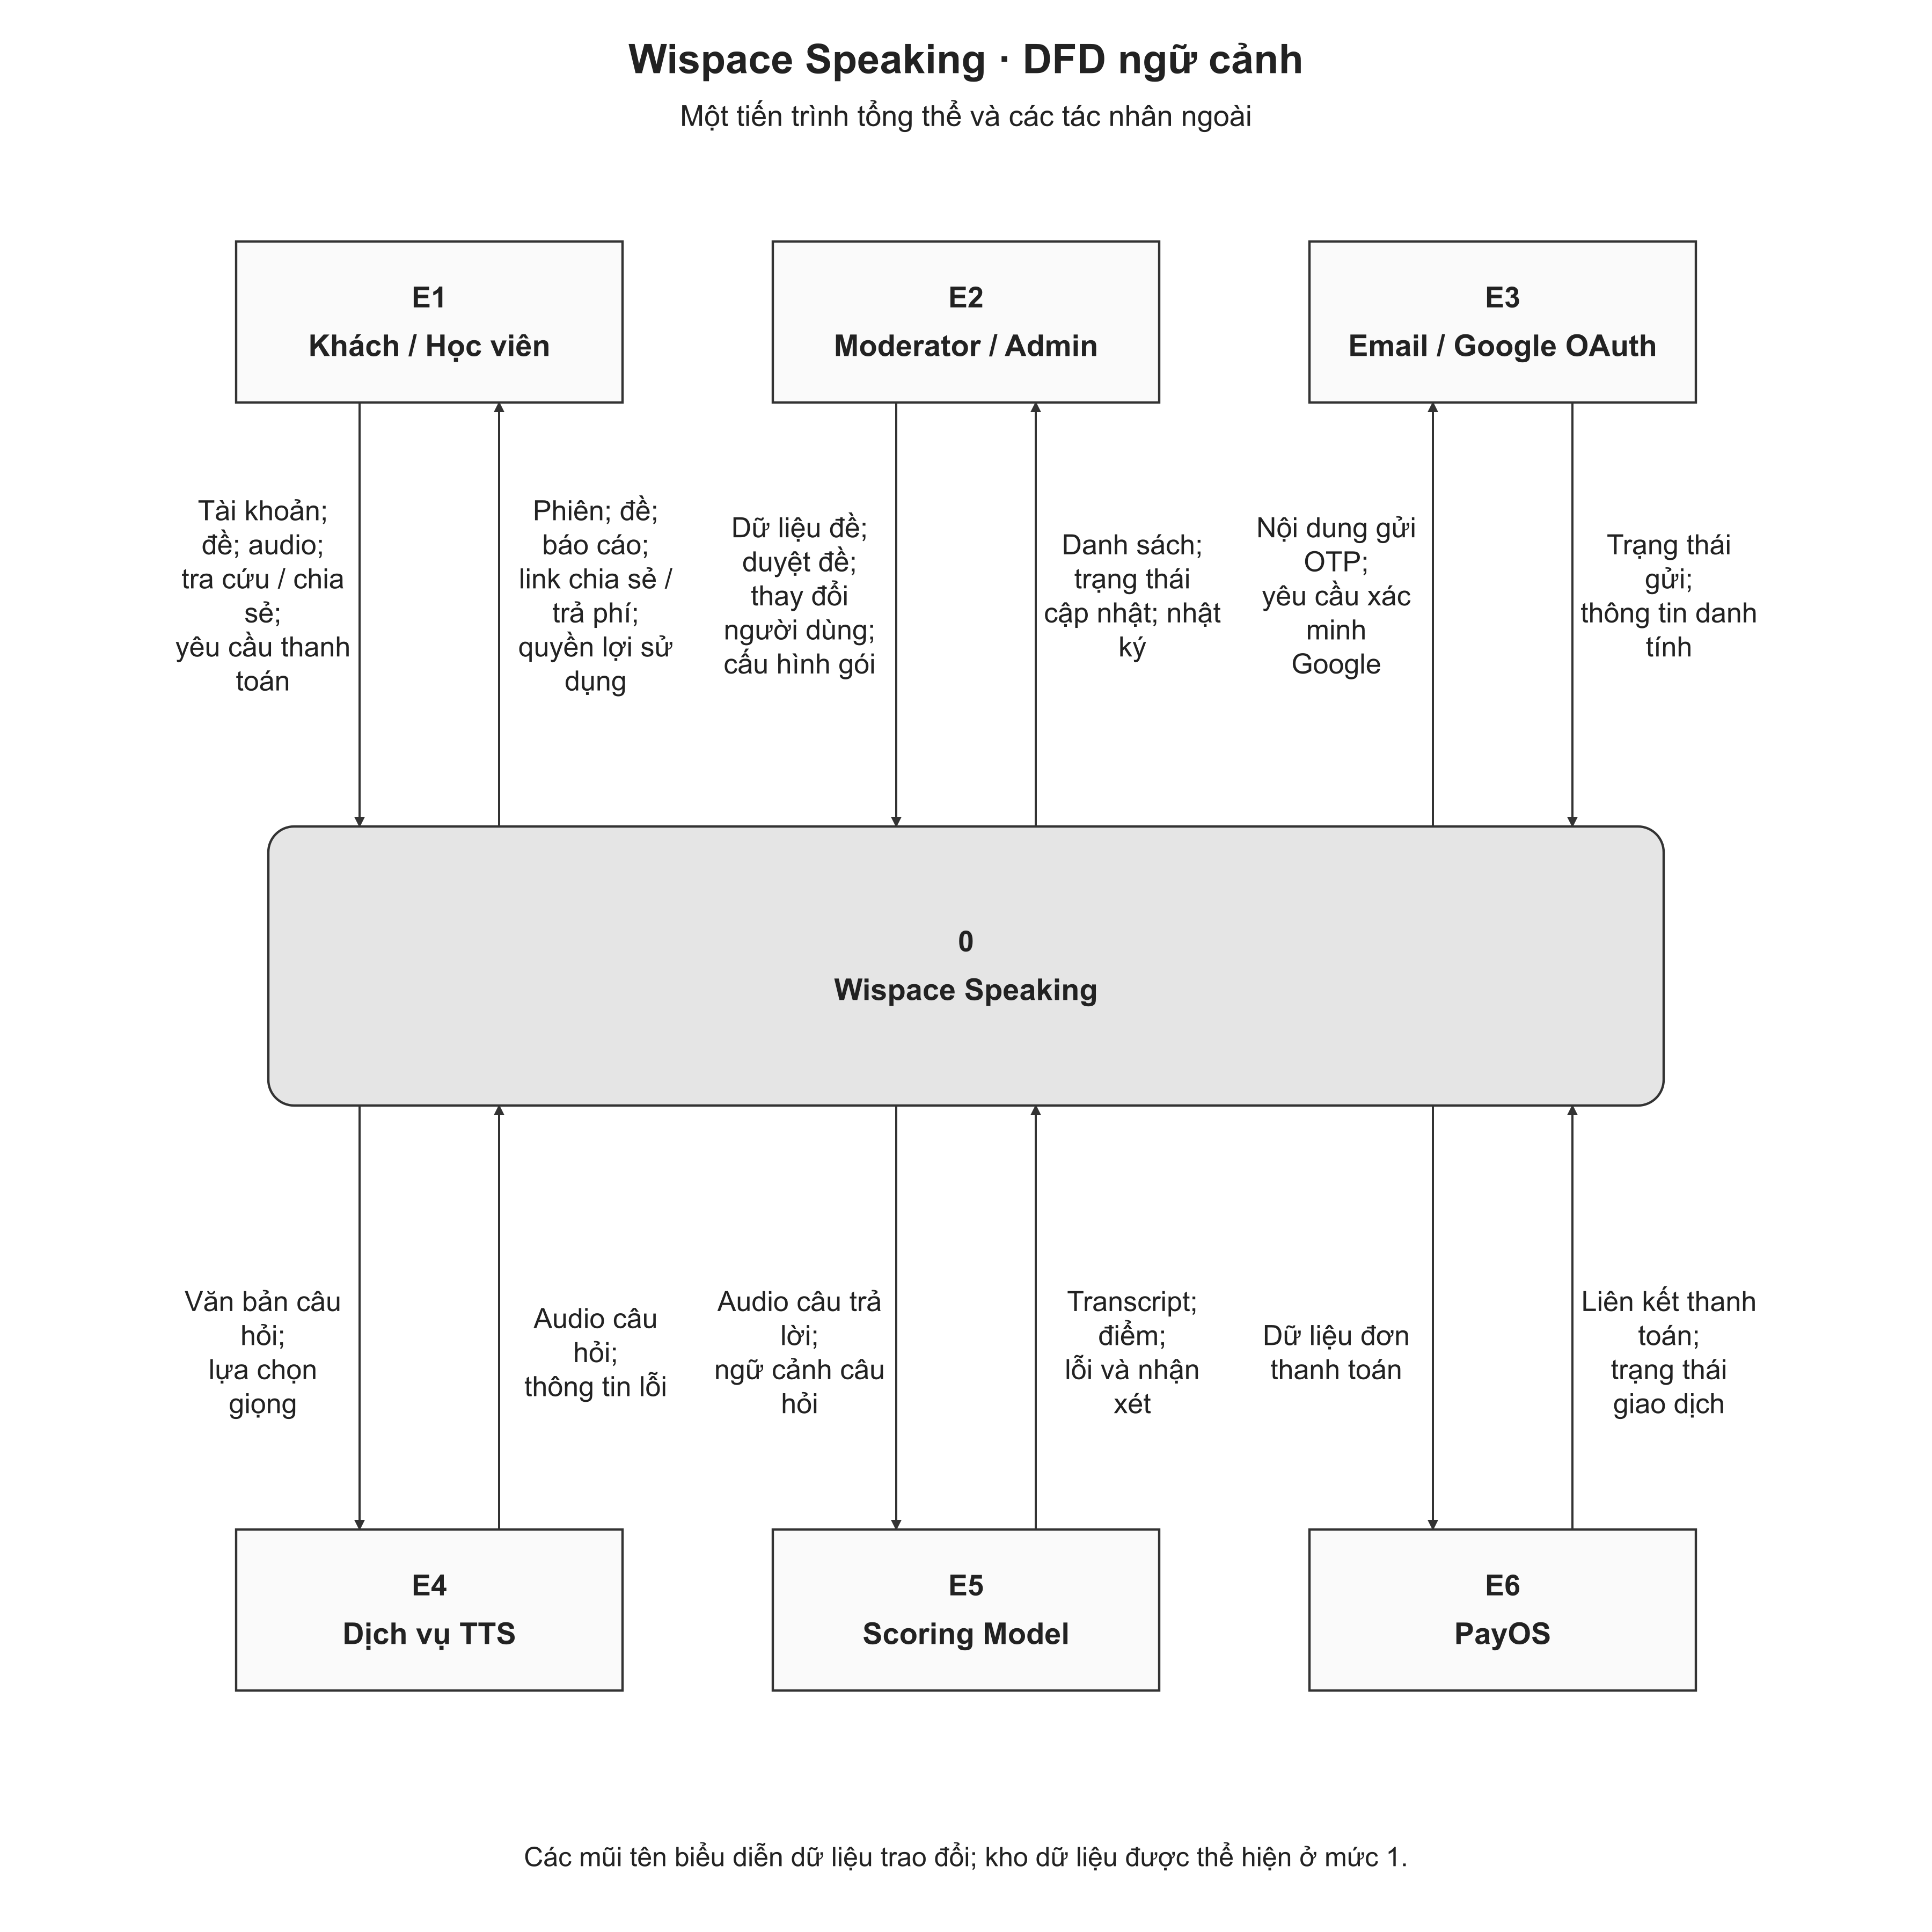
\includegraphics[width=\linewidth,height=0.78\textheight,keepaspectratio]{Images/DFD/Wispace/wispace_dfd_context.png}
\caption{DFD ngữ cảnh của Wispace Speaking}
\label{wispace:fig:dfd-context}
\end{figure}

\clearpage


\paragraph{Sơ đồ mức 1.}

Để giữ nhãn và đường nối dễ đọc, cùng một sơ đồ mức 1 được trình bày thành hai phần. Các tác nhân và kho dữ liệu có cùng mã ở hai phần là cùng một đối tượng logic. Dữ liệu giữa các nhóm xử lý được trao đổi qua kho dùng chung, không phải các bản sao tách biệt.

\clearpage

\begin{figure}[H]
\centering
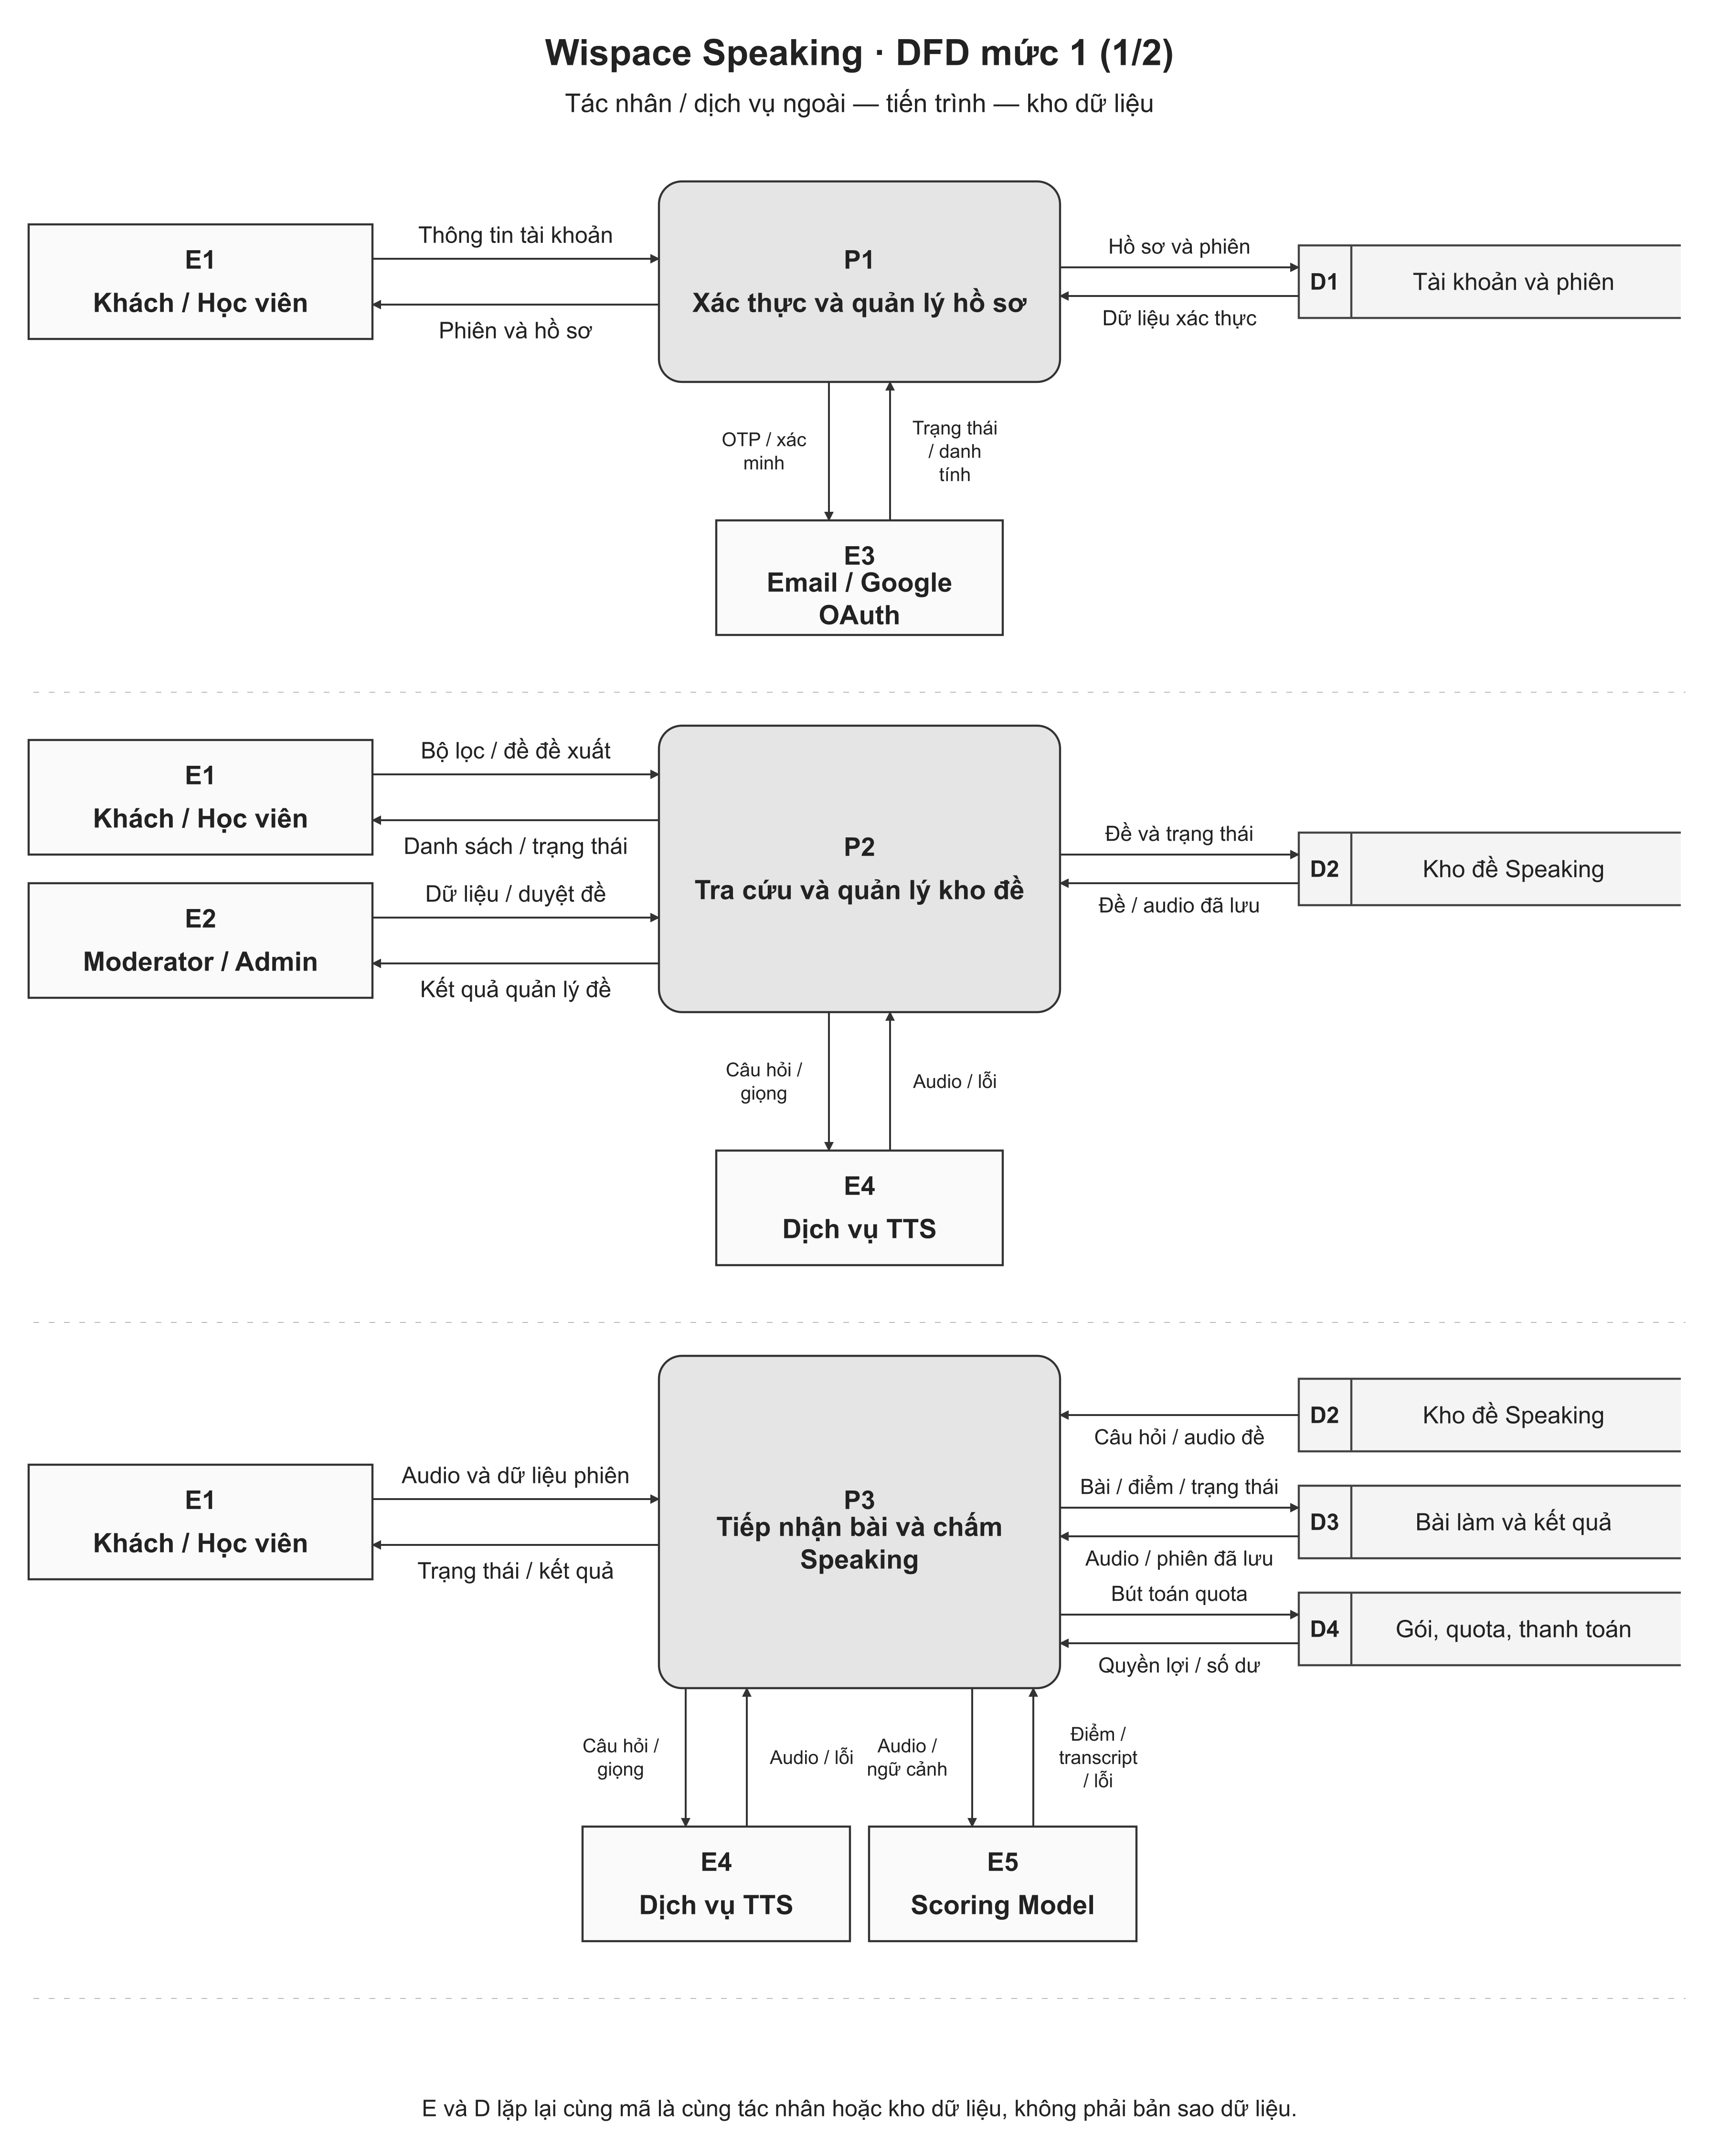
\includegraphics[width=\linewidth,height=0.78\textheight,keepaspectratio]{Images/DFD/Wispace/wispace_dfd_level1_1.png}
\caption{DFD mức 1 của Wispace Speaking: P1, P2, P3}
\label{wispace:fig:dfd-level1-1}
\end{figure}

\clearpage

\begin{figure}[H]
\centering
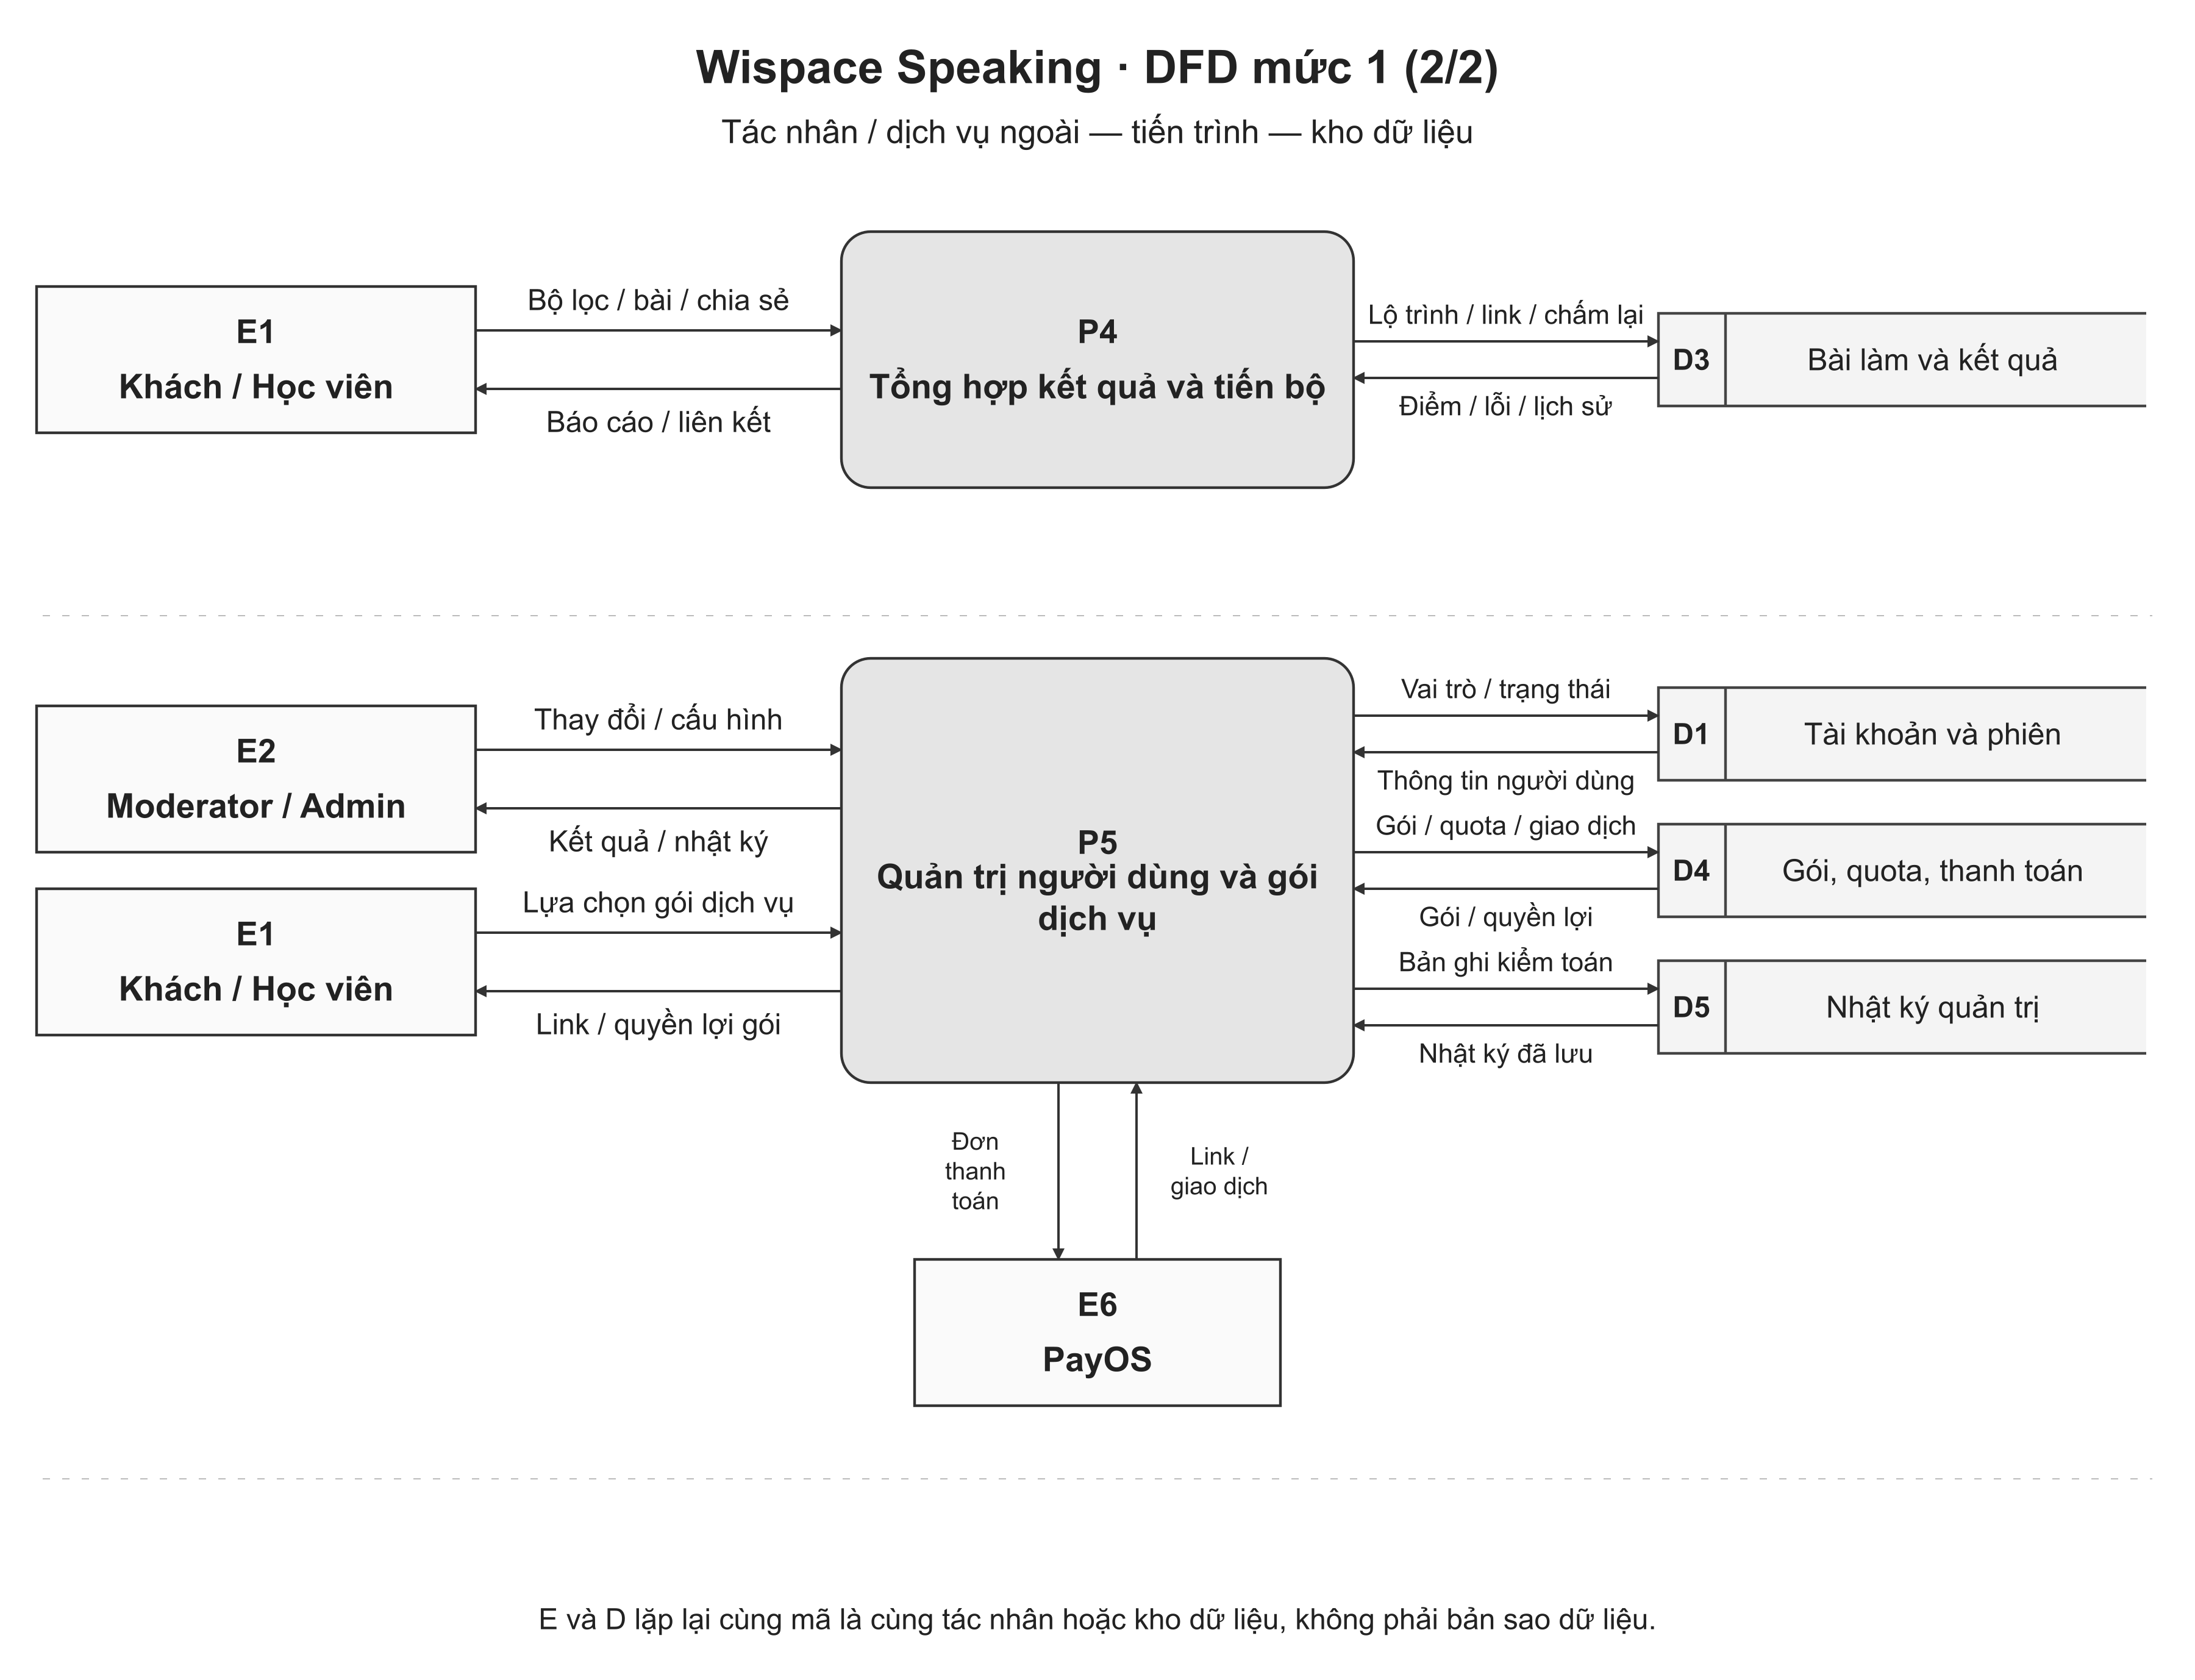
\includegraphics[width=\linewidth,height=0.78\textheight,keepaspectratio]{Images/DFD/Wispace/wispace_dfd_level1_2.png}
\caption{DFD mức 1 của Wispace Speaking: P4, P5}
\label{wispace:fig:dfd-level1-2}
\end{figure}




P3 đọc câu hỏi từ D2, ghi audio và kết quả vào D3, đồng thời cập nhật bút toán quota ở D4. P4 dùng dữ liệu D3 để lập báo cáo, thống kê tiến bộ và quản lý liên kết chia sẻ; yêu cầu chấm lại được ghi vào trạng thái bài làm ở D3 để P3 xử lý. P5 bao gồm yêu cầu mua gói đã nêu ở Chương 5, ngoài phạm vi 12 use-case chi tiết.


\clearpage
\subsection{Hệ thống AIHub}

\subsubsection{Lược đồ Use-case tổng quan}
Toàn bộ hệ thống AIHub bao gồm 20 use-case chính, được phân chia thành 3 phân vùng chức năng cốt lõi như minh họa tại Hình~\ref{aihub:fig:aihub_usecase_overview}:
\textbf{Phân hệ Cổng API Gateway \& Developer Portal:} Bao gồm các chức năng Đăng nhập/Xác thực, Quản lý khóa API, Tra cứu hạn mức và sử dụng cURL Sandbox. \textbf{Phân hệ Quản trị \& Điều hành:} Bao gồm Quản lý thành viên tổ chức, Cấu hình gói và hạn mức, Quản lý danh mục đặc tả Universal Specs, Kiểm tra trạng thái hệ thống và Xem nhật ký kiểm toán.
\begin{figure}[H]
    \centering
    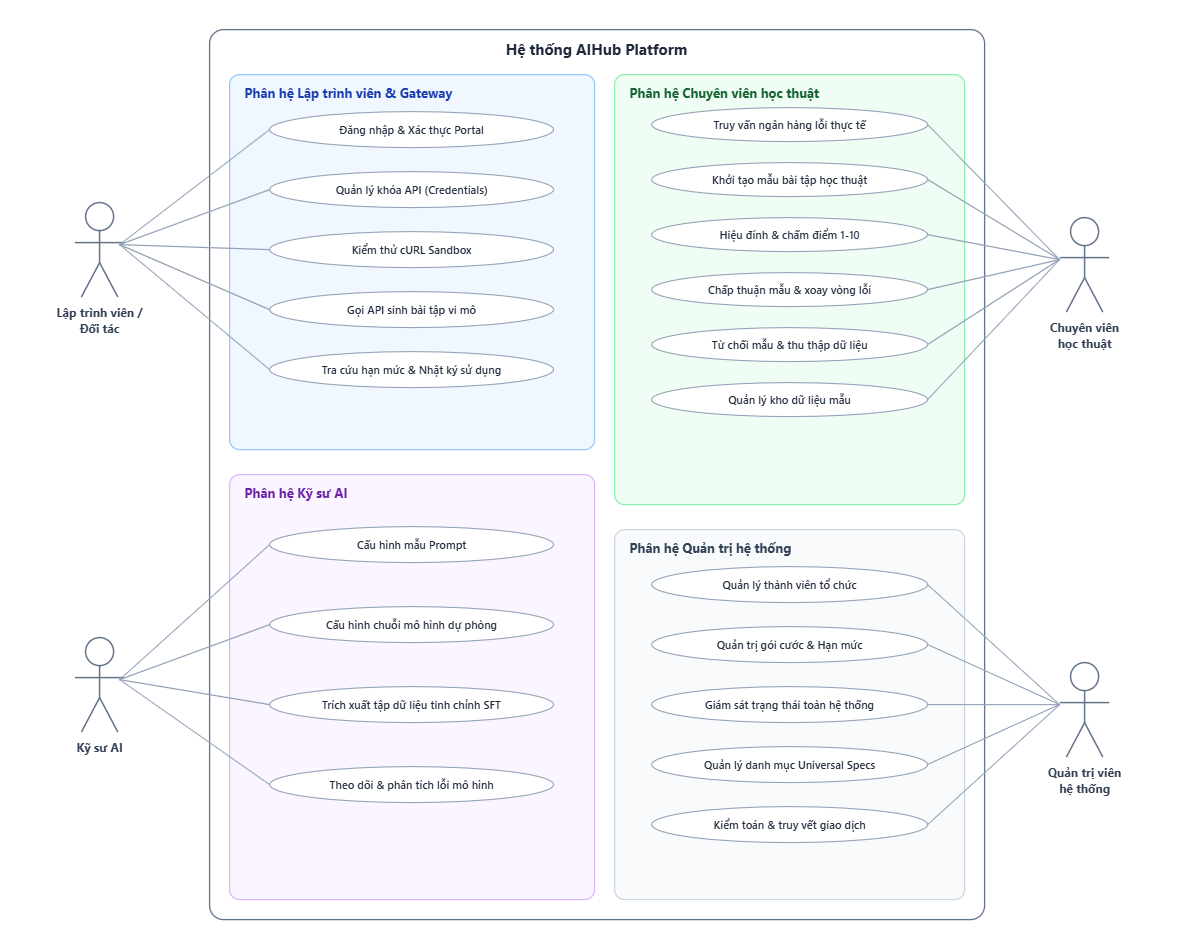
\includegraphics[width=1\textwidth]{Images/Usecase/AIHub/aihub_usecase.png}
    \caption{Sơ đồ Use-case tổng quan hệ thống AIHub Platform}
    \label{aihub:fig:aihub_usecase_overview}
\end{figure}
\newpage

\subsubsection{Đặc tả các Use-case chi tiết}
\setcounter{paragraph}{0}                      % Đặt lại bộ đếm về 0
\renewcommand{\theparagraph}{\alph{paragraph}}  % Chuyển số thành chữ cái thường a, b, c...

Các bảng dưới đây đặc tả 20 use-case của AIHub. Mỗi bảng mô tả tác nhân, điều kiện trước và sau, luồng chính, luồng thay thế và các trường hợp ngoại lệ.

% =========================================================================
% NHÓM 1: LẬP TRÌNH VIÊN / ĐỐI TÁC TÍCH HỢP
% =========================================================================

\paragraph{Use-case 1: Đăng nhập và Xác thực Portal}

\begingroup
\small
\begin{longtable}{|p{3.2cm}|p{\dimexpr\linewidth-3.2cm-4\tabcolsep-3\arrayrulewidth\relax}|}
\caption{Đặc tả use-case Đăng nhập và Xác thực Portal}
\label{aihub:tab:uc_dev_auth}\\
\hline
\textbf{Tác nhân} & Lập trình viên / Đối tác tích hợp, Máy chủ xác thực (Session Service) \\ \hline
\textbf{Điều kiện trước} & Hệ thống hoạt động bình thường; lập trình viên đã có tài khoản được kích hoạt trong bảng \texttt{users}. \\ \hline
\textbf{Điều kiện sau} & Phiên làm việc được thiết lập qua Session Cookie an toàn; lập trình viên được chuyển tới Bảng điều khiển nhà phát triển. \\ \hline
\textbf{Luồng chính} & 1. Người dùng mở Portal, nhập email và mật khẩu.\newline 2. Hệ thống kiểm tra đầu vào, mật khẩu băm, trạng thái tài khoản, vai trò và tổ chức.\newline 3. Hệ thống tạo phiên bằng cookie bảo mật và mở Dashboard. \\ \hline
\textbf{Luồng thay thế} &
\textbf{Nhánh 1: Đăng xuất khỏi hệ thống (Logout)}\newline 1.1. Lập trình viên chọn menu tài khoản và nhấn ``Đăng xuất''.\newline 1.2. Hệ thống thu hồi phiên làm việc, xóa cookie bảo mật trên trình duyệt và điều hướng về trang đăng nhập. \\ \hline
\textbf{Ngoại lệ} &
\textbf{Lỗi 1: Sai email hoặc mật khẩu}\newline Hệ thống hiển thị thông báo ``Thông tin đăng nhập không hợp lệ''. Nhập sai quá 5 lần liên tiếp sẽ tạm khóa tài khoản 15 phút.\newline \textbf{Lỗi 2: Tài khoản bị khóa}\newline Trả về thông báo tài khoản đang bị vô hiệu hóa kèm chỉ dẫn liên hệ Quản trị viên. \\ \hline
\end{longtable}
\endgroup
\paragraph{Use-case 2: Quản lý khóa API}

\begingroup
\small
\begin{longtable}{|p{3.2cm}|p{\dimexpr\linewidth-3.2cm-4\tabcolsep-3\arrayrulewidth\relax}|}
\caption{Đặc tả use-case Quản lý khóa API}
\label{aihub:tab:uc_manage_credentials}\\
\hline
\textbf{Tác nhân} & Lập trình viên, Quản trị viên tổ chức \\ \hline
\textbf{Điều kiện trước} & Người dùng đã đăng nhập với vai trò hợp lệ trong tổ chức. \\ \hline
\textbf{Điều kiện sau} & Cặp mã chứng thực được cập nhật trong bảng \texttt{credentials}; khóa bí mật mới chỉ được hiển thị duy nhất 1 lần. \\ \hline
\textbf{Luồng chính} & 1. Người dùng chọn tạo hoặc xoay vòng khóa.\newline 2. Hệ thống kiểm tra quyền và giới hạn gói, sinh clientId có tiền tố môi trường và secretKey ngẫu nhiên.\newline 3. Bí mật được băm bằng Bcrypt; credentials được lưu theo tổ chức.\newline 4. Hệ thống hiển thị bí mật một lần để người dùng sao chép và xác nhận. \\ \hline
\textbf{Luồng thay thế} &
\textbf{Nhánh 1: Thu hồi hoặc vô hiệu hóa khóa (Revoke Key)}\newline Lập trình viên chọn một khóa đang hoạt động và nhấn ``Xóa khóa''. Hệ thống đánh dấu vô hiệu hóa; mọi yêu cầu sử dụng khóa này sẽ bị Gateway từ chối ngay lập tức. \\ \hline
\textbf{Ngoại lệ} &
\textbf{Lỗi 1: Vượt quá số lượng khóa cho phép của gói cước}\newline Nếu tổ chức thuộc gói Free Sandbox và đã đạt giới hạn 2 khóa, hệ thống từ chối tạo mới và yêu cầu nâng cấp gói cước. \\ \hline
\end{longtable}
\endgroup

\paragraph{Use-case 3: Kiểm thử cURL Sandbox}

\begingroup
\small
\begin{longtable}{|p{3.2cm}|p{\dimexpr\linewidth-3.2cm-4\tabcolsep-3\arrayrulewidth\relax}|}
\caption{Đặc tả use-case Kiểm thử cURL Sandbox}
\label{aihub:tab:uc_run_spec_curl}\\
\hline
\textbf{Tác nhân} & Lập trình viên / Đối tác tích hợp \\ \hline
\textbf{Điều kiện trước} & Lập trình viên đã mở trang Universal AI Spec Catalog; đặc tả dịch vụ đã được tải. \\ \hline
\textbf{Điều kiện sau} & Nhận kết quả phản hồi JSON, thời gian xử lý (latency), số token tiêu thụ và trạng thái kiểm định tính hợp lệ của lược đồ. \\ \hline
\textbf{Luồng chính} & 1. Lập trình viên chọn dịch vụ, xem đặc tả và nhập JSON yêu cầu.\newline 2. Hệ thống thực thi dịch vụ nội bộ; dịch vụ đối tác chưa tích hợp dùng mô phỏng có kiểm định schema với độ trễ 300--800 ms.\newline 3. Hệ thống hiển thị mã HTTP, JSON, thời gian xử lý, token và kết quả kiểm định schema. \\ \hline
\textbf{Luồng thay thế} & Không có. \\ \hline
\textbf{Ngoại lệ} &
\textbf{Lỗi 1: Dữ liệu JSON gửi đi sai cú pháp}\newline Giao diện cảnh báo lỗi cú pháp JSON và khóa nút gửi yêu cầu.\newline \textbf{Lỗi 2: Cấu trúc phản hồi không khớp lược đồ chuẩn}\newline Hệ thống hiển thị cờ cảnh báo \texttt{validation.valid = false} kèm danh sách chi tiết các trường bị thiếu hoặc sai kiểu dữ liệu. \\ \hline
\end{longtable}
\endgroup

\paragraph{Use-case 4: Gọi API sinh bài tập vi mô}

\begingroup
\small
\begin{longtable}{|p{3.2cm}|p{\dimexpr\linewidth-3.2cm-4\tabcolsep-3\arrayrulewidth\relax}|}
\caption{Đặc tả use-case Gọi API sinh bài tập vi mô}
\label{aihub:tab:uc_create_exercise}\\
\hline
\textbf{Tác nhân} & Ứng dụng WISPACE / Lập trình viên, Composite LLM Adapter \\ \hline
\textbf{Điều kiện trước} & Header yêu cầu chứa mã \textit{x-client-id} và \textit{x-secret-key} hợp lệ; tổ chức còn hạn ngạch gọi API trong tháng. \\ \hline
\textbf{Điều kiện sau} & Bài tập được khởi tạo hoàn chỉnh với câu hỏi, đáp án, giải thích chi tiết và rubric chấm điểm; số liệu được ghi vào \texttt{usage\_logs}. \\ \hline
\textbf{Luồng chính} & 1. Gateway xác thực credentials, quyền dịch vụ, RPM và hạn mức.\newline 2. Hệ thống kiểm tra dữ liệu và mã lỗi trong bộ 28 lỗi IELTS.\newline 3. Hệ thống lấy dẫn chứng theo chủ đề, gọi mô hình sinh bài tập và chuẩn hóa kết quả.\newline 4. Phản hồi gồm câu hỏi, đáp án, giải thích, rubric và metadata mô hình/thời gian/token; usage được ghi nhận. \\ \hline
\textbf{Luồng thay thế} &
\textbf{Nhánh 1: Sinh dạng bài tự luận ngắn (Short Writing)}\newline Hệ thống tự động đính kèm tiêu chí chấm điểm chi tiết \textit{ai\_grading\_rubric} trên thang điểm 1--10 và câu trả lời mẫu chuẩn Band 8.0+. \\ \hline
\textbf{Ngoại lệ} &
\textbf{Lỗi 1: Mã lỗi không thuộc bộ phân loại 28 lỗi IELTS}\newline Ném lỗi miền \texttt{InvalidErrorCodeError}, trả về mã HTTP 400 Bad Request.\newline \textbf{Lỗi 2: Dịch vụ AI chính gặp sự cố kết nối hoặc quá thời gian chờ}\newline Kích hoạt chuỗi dự phòng (Fallback Chain): tự động chuyển sang Google Gemini $\rightarrow$ OpenAI GPT-4o $\rightarrow$ Động cơ Ngoại tuyến (Deterministic Engine). \\ \hline
\end{longtable}
\endgroup

\paragraph{Use-case 5: Tra cứu hạn mức và Nhật ký sử dụng}

\begingroup
\small
\begin{longtable}{|p{3.2cm}|p{\dimexpr\linewidth-3.2cm-4\tabcolsep-3\arrayrulewidth\relax}|}
\caption{Đặc tả use-case Tra cứu hạn mức và Nhật ký sử dụng}
\label{aihub:tab:uc_view_usage_logs}\\
\hline
\textbf{Tác nhân} & Lập trình viên, Quản trị viên tổ chức \\ \hline
\textbf{Điều kiện trước} & Người dùng đã đăng nhập và thuộc một tổ chức có mã khóa truy cập. \\ \hline
\textbf{Điều kiện sau} & Bảng chỉ số tiêu thụ, biểu đồ trực quan và nhật ký giao dịch được hiển thị đầy đủ. \\ \hline
\textbf{Luồng chính} & 1. Người dùng mở mục sử dụng dịch vụ.\newline 2. Hệ thống hiển thị hạn mức tháng đã dùng/còn lại và trần RPM.\newline 3. Hệ thống tổng hợp lưu lượng, mã HTTP, độ trễ và token theo ngày.\newline 4. Người dùng xem nhật ký gồm thời điểm, endpoint, phương thức, thời lượng, token, IP và trạng thái. \\ \hline
\textbf{Luồng thay thế} &
\textbf{Nhánh 1: Lọc nhật ký theo tiêu chí nâng cao}\newline Người dùng lọc danh sách giao dịch theo khoảng ngày, theo mã khóa \textit{clientId} cụ thể, hoặc chỉ hiển thị các yêu cầu gặp lỗi (mã $4xx$, $5xx$). \\ \hline
\textbf{Ngoại lệ} &
\textbf{Lỗi 1: Định ngạch chạm ngưỡng cảnh báo ($\ge 80\%$ hoặc $100\%$)}\newline Hệ thống hiển thị thanh thông báo màu đỏ cảnh báo tổ chức sắp hoặc đã dùng hết định ngạch gọi API trong tháng, đề xuất nâng cấp gói cước. \\ \hline
\end{longtable}
\endgroup

% =========================================================================
% NHÓM 2: CHUYÊN VIÊN HỌC THUẬT (ACADEMIC LAB)
% =========================================================================

\paragraph{Use-case 6: Truy vấn ngân hàng lỗi thực tế}

\begingroup
\small
\begin{longtable}{|p{3.2cm}|p{\dimexpr\linewidth-3.2cm-4\tabcolsep-3\arrayrulewidth\relax}|}
\caption{Đặc tả use-case Truy vấn ngân hàng lỗi thực tế}
\label{aihub:tab:uc_query_references}\\
\hline
\textbf{Tác nhân} & Chuyên viên học thuật, WISPACE Reference API / DB Adapter \\ \hline
\textbf{Điều kiện trước} & Chuyên viên đã đăng nhập vào Academic Lab Workbench; kho dẫn chứng khả dụng. \\ \hline
\textbf{Điều kiện sau} & Danh sách các trích dẫn lỗi bài thi kèm đề bài và nhận xét chuyên môn được trả về. \\ \hline
\textbf{Luồng chính} & 1. Chuyên viên chọn Task 1/2, tiêu chí TR/CC/LR/GRA, mã lỗi, chủ đề và số dẫn chứng.\newline 2. Hệ thống kiểm tra tham số và truy vấn API dẫn chứng Wispace.\newline 3. Kết quả gồm đề bài, loại câu hỏi, trích dẫn, ảnh biểu đồ nếu có và nhận xét chuyên môn.\newline 4. Hệ thống chuẩn hóa và hiển thị dẫn chứng. \\ \hline
\textbf{Luồng thay thế} &
\textbf{Nhánh 1: Kết nối API ngoài gián đoạn, kích hoạt kho dẫn chứng nội bộ}\newline Nếu gọi API WISPACE thất bại hoặc quá thời gian chờ, hệ thống tự động chuyển sang \texttt{WispaceReferenceAdapter} để truy vấn trực tiếp từ bảng cơ sở dữ liệu cục bộ \texttt{wispace\_essay\_references} và tiếp tục bước 5. \\ \hline
\textbf{Ngoại lệ} &
\textbf{Lỗi 1: Không tìm thấy dẫn chứng phù hợp}\newline Trả về danh sách rỗng kèm thông báo đề xuất mở rộng phạm vi tìm kiếm hoặc chuyển sang chế độ sinh bài tập không dùng dẫn chứng thực tế. \\ \hline
\end{longtable}
\endgroup

\paragraph{Use-case 7: Khởi tạo mẫu bài tập học thuật}

\begingroup
\small
\begin{longtable}{|p{3.2cm}|p{\dimexpr\linewidth-3.2cm-4\tabcolsep-3\arrayrulewidth\relax}|}
\caption{Đặc tả use-case Khởi tạo mẫu bài tập học thuật}
\label{aihub:tab:uc_academic_generate}\\
\hline
\textbf{Tác nhân} & Chuyên viên học thuật, Composite LLM Adapter \\ \hline
\textbf{Điều kiện trước} & Chuyên viên đã đăng nhập hệ thống với quyền \textit{ACADEMIC\_SPECIALIST}. \\ \hline
\textbf{Điều kiện sau} & Bản ghi mẫu học thuật được tạo ở trạng thái DRAFT; dữ liệu AI thô được lưu trữ nguyên vẹn trong trường \textit{rawAiOutput}. \\ \hline
\textbf{Luồng chính} & 1. Chuyên viên chọn Task, tiêu chí, mã lỗi, dạng bài tập và nhập chỉ dẫn sư phạm.\newline 2. Hệ thống kiểm tra tham số, lấy dẫn chứng nếu được yêu cầu và dựng Prompt theo phiên bản.\newline 3. Mô hình sinh nội dung; hệ thống kiểm tra kết quả.\newline 4. Mẫu được lưu DRAFT với rawAiOutput nguyên vẹn và hiển thị để thẩm định. \\ \hline
\textbf{Luồng thay thế} &
\textbf{Nhánh 1: Sử dụng dẫn chứng tùy biến do chuyên viên nhập}\newline Chuyên viên tự nhập trực tiếp câu trích dẫn và phân tích lỗi của học sinh thay vì lấy tự động từ ngân hàng dữ liệu. \\ \hline
\textbf{Ngoại lệ} &
\textbf{Lỗi 1: Lỗi mô hình AI không tạo được nội dung hợp lệ}\newline Hệ thống hiển thị thông báo lỗi chi tiết, giữ nguyên các tham số cấu hình trên form và đề xuất chuyên viên thử lại. \\ \hline
\end{longtable}
\endgroup

\paragraph{Use-case 8: Kiểm định, hiệu đính và chấm điểm bài tập}

\begingroup
\small
\begin{longtable}{|p{3.2cm}|p{\dimexpr\linewidth-3.2cm-4\tabcolsep-3\arrayrulewidth\relax}|}
\caption{Đặc tả use-case Kiểm định, hiệu đính và chấm điểm bài tập}
\label{aihub:tab:uc_academic_review_score}\\
\hline
\textbf{Tác nhân} & Chuyên viên học thuật \\ \hline
\textbf{Điều kiện trước} & Mẫu bài tập đang mở ở trạng thái DRAFT; đã có dữ liệu \textit{rawAiOutput}. \\ \hline
\textbf{Điều kiện sau} & Bản hiệu đính hoàn chỉnh được lưu tạm trong trường \textit{finalOutput} kèm điểm số chất lượng (1--10). \\ \hline
\textbf{Luồng chính} & 1. Chuyên viên kiểm tra câu hỏi, đáp án và giải thích trong rawAiOutput.\newline 2. Chuyên viên hiệu đính finalOutput, nhập điểm chất lượng bản gốc 1--10 và reviewedBy.\newline 3. Hệ thống tự lưu bản nháp; quyết định duyệt được thực hiện riêng. \\ \hline
\textbf{Luồng thay thế} &
\textbf{Nhánh 1: Bản sinh AI đã đạt độ hoàn hảo, không cần chỉnh sửa}\newline Chuyên viên nhấn nút ``Sao chép nguyên bản'', hệ thống tự động đồng bộ toàn bộ nội dung từ \textit{rawAiOutput} sang \textit{finalOutput}. \\ \hline
\textbf{Ngoại lệ} &
\textbf{Lỗi 1: Điểm số nhập vào không hợp lệ}\newline Nếu điểm số nằm ngoài dải giá trị từ 1 đến 10 hoặc không phải là số nguyên, hệ thống báo đỏ ô nhập liệu và ngăn thao tác phê duyệt. \\ \hline
\end{longtable}
\endgroup

\paragraph{Use-case 9: Chấp thuận mẫu và xoay vòng lỗi}

\begingroup
\small
\begin{longtable}{|p{3.2cm}|p{\dimexpr\linewidth-3.2cm-4\tabcolsep-3\arrayrulewidth\relax}|}
\caption{Đặc tả use-case Chấp thuận mẫu và xoay vòng lỗi}
\label{aihub:tab:uc_academic_accept}\\
\hline
\textbf{Tác nhân} & Chuyên viên học thuật, Cơ sở dữ liệu PostgreSQL \\ \hline
\textbf{Điều kiện trước} & Mẫu bài tập đang ở trạng thái DRAFT; khung \textit{finalOutput} không để trống và điểm số đã được nhập hợp lệ. \\ \hline
\textbf{Điều kiện sau} & Mẫu chuyển sang trạng thái ACCEPTED; cặp dữ liệu chuẩn vàng được bảo toàn; giao diện chuyển sang cấu hình bài tập tiếp theo. \\ \hline
\textbf{Luồng chính} & 1. Chuyên viên xác nhận chấp thuận mẫu DRAFT có bản hiệu đính và điểm hợp lệ.\newline 2. Hệ thống giữ bản gốc, lưu finalOutput, điểm và người thẩm định; chuyển trạng thái ACCEPTED.\newline 3. Hệ thống chọn mã lỗi/chủ đề tiếp theo từ lịch sử và ma trận 28 mã lỗi, rồi điền cấu hình cho lượt sinh mới. \\ \hline
\textbf{Luồng thay thế} &
\textbf{Nhánh 1: Đánh dấu mẫu yêu thích đặc biệt}\newline Chuyên viên tích chọn ``Mẫu chuẩn mực (Favorite)'', hệ thống gán cờ \textit{isFavorite = true} để ưu tiên trích xuất tập dữ liệu huấn luyện mẫu mực. \\ \hline
\textbf{Ngoại lệ} &
\textbf{Lỗi 1: Xung đột phiên chỉnh sửa dữ liệu}\newline Nếu bản ghi đã bị sửa đổi bởi một chuyên viên khác trước đó, hệ thống cảnh báo xung đột và tải lại trạng thái dữ liệu mới nhất. \\ \hline
\end{longtable}
\endgroup

\paragraph{Use-case 10: Từ chối mẫu và thu thập dữ liệu tinh chỉnh}

\begingroup
\small
\begin{longtable}{|p{3.2cm}|p{\dimexpr\linewidth-3.2cm-4\tabcolsep-3\arrayrulewidth\relax}|}
\caption{Đặc tả use-case Từ chối mẫu và thu thập dữ liệu tinh chỉnh}
\label{aihub:tab:uc_academic_reject}\\
\hline
\textbf{Tác nhân} & Chuyên viên học thuật, Kỹ sư AI \\ \hline
\textbf{Điều kiện trước} & Mẫu bài tập đang mở ở trạng thái DRAFT. \\ \hline
\textbf{Điều kiện sau} & Bản ghi chuyển sang trạng thái REJECTED kèm lý do chi tiết; mẫu được gắn nhãn đưa vào tập dữ liệu mẫu âm. \\ \hline
\textbf{Luồng chính} & 1. Chuyên viên chọn từ chối, nhập lý do chuyên môn và xác nhận.\newline 2. Hệ thống lưu rejectReason, chuyển mẫu sang REJECTED và đưa vào kho phân tích mẫu lỗi.\newline 3. Giao diện cho phép sinh mẫu mới với ngữ cảnh tránh lỗi đã ghi nhận. \\ \hline
\textbf{Luồng thay thế} & Không có. \\ \hline
\textbf{Ngoại lệ} &
\textbf{Lỗi 1: Để trống lý do từ chối}\newline Hệ thống yêu cầu bắt buộc phải nhập tối thiểu 10 ký tự mô tả nguyên nhân bác bỏ nhằm đảm bảo chất lượng dữ liệu phản hồi cho mô hình AI. \\ \hline
\end{longtable}
\endgroup

\paragraph{Use-case 11: Quản lý kho dữ liệu mẫu học thuật}

\begingroup
\small
\begin{longtable}{|p{3.2cm}|p{\dimexpr\linewidth-3.2cm-4\tabcolsep-3\arrayrulewidth\relax}|}
\caption{Đặc tả use-case Quản lý kho dữ liệu mẫu học thuật}
\label{aihub:tab:uc_academic_inventory}\\
\hline
\textbf{Tác nhân} & Chuyên viên học thuật, Kỹ sư AI \\ \hline
\textbf{Điều kiện trước} & Người dùng đã đăng nhập với vai trò \textit{ACADEMIC\_SPECIALIST} hoặc \textit{AI\_ENGINEER}. \\ \hline
\textbf{Điều kiện sau} & Danh sách các mẫu bài tập phân trang được hiển thị đầy đủ kèm trạng thái phê duyệt và điểm số. \\ \hline
\textbf{Luồng chính} & 1. Người dùng mở kho mẫu; hệ thống hiển thị 20 mẫu/trang, mới nhất trước.\newline 2. Người dùng lọc theo DRAFT/ACCEPTED/REJECTED, Task, tiêu chí, mã lỗi, điểm, người thẩm định hoặc yêu thích.\newline 3. Người dùng mở mẫu để đối chiếu rawAiOutput và finalOutput. \\ \hline
\textbf{Luồng thay thế} &
\textbf{Nhánh 1: Đánh dấu nhanh mẫu chuẩn mực}\newline Chuyên viên nhấn biểu tượng ngôi sao để chuyển đổi trạng thái yêu thích (\textit{isFavorite}) của mẫu bài tập. \\ \hline
\textbf{Ngoại lệ} &
\textbf{Lỗi 1: Không có bản ghi phù hợp bộ lọc}\newline Hệ thống hiển thị thông báo ``Không tìm thấy mẫu bài tập phù hợp'' kèm nút đặt lại toàn bộ bộ lọc. \\ \hline
\end{longtable}
\endgroup

% =========================================================================
% NHÓM 3: KỸ SƯ AI
% =========================================================================

\paragraph{Use-case 12: Cấu hình mẫu Prompt}

\begingroup
\small
\begin{longtable}{|p{3.2cm}|p{\dimexpr\linewidth-3.2cm-4\tabcolsep-3\arrayrulewidth\relax}|}
\caption{Đặc tả use-case Cấu hình mẫu Prompt}
\label{aihub:tab:uc_config_prompt}\\
\hline
\textbf{Tác nhân} & Kỹ sư AI \\ \hline
\textbf{Điều kiện trước} & Tài khoản có vai trò \textit{AI\_ENGINEER} hoặc \textit{ADMIN}. \\ \hline
\textbf{Điều kiện sau} & Mẫu prompt mới được lưu và có hiệu lực tức thì cho các lượt sinh bài tiếp theo. \\ \hline
\textbf{Luồng chính} & 1. Kỹ sư chọn nhóm Task, tiêu chí và mã lỗi.\newline 2. Kỹ sư chỉnh System Prompt, biến ngữ cảnh, JSON Schema và ví dụ mẫu.\newline 3. Hệ thống kiểm tra schema và biến bắt buộc, lưu phiên bản mới và cập nhật cấu hình thực thi. \\ \hline
\textbf{Luồng thay thế} &
\textbf{Nhánh 1: Thử nghiệm Prompt với dữ liệu giả lập (Dry Run)}\newline Kỹ sư nhấn ``Chạy thử nghiệm Prompt'', hệ thống gửi lệnh tới mô hình với dữ liệu mẫu và hiển thị kết quả JSON trả về để đánh giá chất lượng trước khi lưu. \\ \hline
\textbf{Ngoại lệ} &
\textbf{Lỗi 1: Cú pháp JSON Schema bị lỗi}\newline Hệ thống bắt lỗi biên dịch schema, từ chối lưu và bôi đỏ vị trí sai cú pháp. \\ \hline
\end{longtable}
\endgroup

\paragraph{Use-case 13: Cấu hình chuỗi mô hình dự phòng}

\begingroup
\small
\begin{longtable}{|p{3.2cm}|p{\dimexpr\linewidth-3.2cm-4\tabcolsep-3\arrayrulewidth\relax}|}
\caption{Đặc tả use-case Cấu hình chuỗi mô hình dự phòng}
\label{aihub:tab:uc_config_fallback}\\
\hline
\textbf{Tác nhân} & Kỹ sư AI, Hệ thống AI Gateway \\ \hline
\textbf{Điều kiện trước} & Tài khoản có quyền \textit{AI\_ENGINEER}. \\ \hline
\textbf{Điều kiện sau} & Quy tắc định tuyến dự phòng đa tầng được cập nhật vào \texttt{CompositeLLMAdapter}. \\ \hline
\textbf{Luồng chính} & 1. Kỹ sư mở cấu hình và xem các nhà cung cấp hiện có.\newline 2. Kỹ sư thiết lập thứ tự Wispace AI, Gemini, OpenAI và động cơ xác định; cấu hình trạng thái sử dụng, timeout và số lần thử lại.\newline 3. Hệ thống kiểm tra kết nối, lưu và áp dụng chuỗi dự phòng cho các yêu cầu tiếp theo. \\ \hline
\textbf{Luồng thay thế} &
\textbf{Nhánh 1: Tạm ngắt kết nối một nhà cung cấp}\newline Kỹ sư AI tắt nút kích hoạt của một mô hình đang gặp sự cố; hệ thống tự động bỏ qua cấp đó trong chuỗi dự phòng. \\ \hline
\textbf{Ngoại lệ} &
\textbf{Lỗi 1: Không có nhà cung cấp nào được kích hoạt}\newline Hệ thống cảnh báo bắt buộc phải duy trì ít nhất một nhà cung cấp đám mây và động cơ ngoại tuyến Deterministic Engine. \\ \hline
\end{longtable}
\endgroup

\paragraph{Use-case 14: Trích xuất tập dữ liệu tinh chỉnh SFT/DPO}

\begingroup
\small
\begin{longtable}{|p{3.2cm}|p{\dimexpr\linewidth-3.2cm-4\tabcolsep-3\arrayrulewidth\relax}|}
\caption{Đặc tả use-case Trích xuất tập dữ liệu tinh chỉnh SFT/DPO}
\label{aihub:tab:uc_export_datasets}\\
\hline
\textbf{Tác nhân} & Kỹ sư AI, PostgreSQL Database \\ \hline
\textbf{Điều kiện trước} & Người dùng có quyền \textit{AI\_ENGINEER}; kho mẫu bài tập có dữ liệu đã thẩm định. \\ \hline
\textbf{Điều kiện sau} & Tập tin dữ liệu huấn luyện định dạng JSONL được nén và sẵn sàng tải xuống. \\ \hline
\textbf{Luồng chính} & 1. Kỹ sư chọn SFT hoặc DPO và bộ lọc thời gian, Task, tiêu chí.\newline 2. SFT lấy mẫu ACCEPTED có điểm $\ge 8.0$, ghép Prompt và finalOutput; DPO lấy Prompt cùng cặp đầu ra được chọn/bị từ chối phù hợp.\newline 3. Tác vụ nền loại thông tin định danh, chuẩn hóa dữ liệu và đóng gói JSONL.\newline 4. Hệ thống hiển thị số mẫu và liên kết tải tệp \texttt{.jsonl.gz}. \\ \hline
\textbf{Luồng thay thế} & Không có. \\ \hline
\textbf{Ngoại lệ} &
\textbf{Lỗi 1: Số lượng mẫu hợp lệ quá ít ($< 50$ mẫu)}\newline Hệ thống cảnh báo kích thước tập dữ liệu chưa đủ độ tin cậy để tinh chỉnh mô hình, đề xuất tiếp tục thẩm định thêm mẫu. \\ \hline
\end{longtable}
\endgroup

\paragraph{Use-case 15: Theo dõi và phân tích lỗi mô hình}

\begingroup
\small
\begin{longtable}{|p{3.2cm}|p{\dimexpr\linewidth-3.2cm-4\tabcolsep-3\arrayrulewidth\relax}|}
\caption{Đặc tả use-case Theo dõi và phân tích lỗi mô hình}
\label{aihub:tab:uc_analyze_model_errors}\\
\hline
\textbf{Tác nhân} & Kỹ sư AI \\ \hline
\textbf{Điều kiện trước} & Tài khoản có quyền \textit{AI\_ENGINEER}. \\ \hline
\textbf{Điều kiện sau} & Báo cáo phân tích chất lượng sinh bài tập và danh sách các lỗi điển hình được trực quan hóa. \\ \hline
\textbf{Luồng chính} & 1. Kỹ sư mở trang phân tích mô hình.\newline 2. Hệ thống tổng hợp tỷ lệ chấp thuận/từ chối, phân bố lý do và ma trận 28 mã lỗi.\newline 3. Kỹ sư xem các mẫu sai band, phương án nhập nhằng hoặc JSON không hợp lệ để điều chỉnh Prompt và dữ liệu. \\ \hline
\textbf{Luồng thay thế} & Không có. \\ \hline
\textbf{Ngoại lệ} & Không có. \\ \hline
\end{longtable}
\endgroup

% =========================================================================
% NHÓM 4: QUẢN TRỊ VIÊN (TỔ CHỨC & NỀN TẢNG)
% =========================================================================

\paragraph{Use-case 16: Quản lý thành viên tổ chức}

\begingroup
\small
\begin{longtable}{|p{3.2cm}|p{\dimexpr\linewidth-3.2cm-4\tabcolsep-3\arrayrulewidth\relax}|}
\caption{Đặc tả use-case Quản lý thành viên tổ chức}
\label{aihub:tab:uc_manage_org_members}\\
\hline
\textbf{Tác nhân} & Quản trị viên tổ chức (Organization Administrator) \\ \hline
\textbf{Điều kiện trước} & Người dùng có vai trò \textit{OWNER} hoặc \textit{ADMIN} trong bảng \texttt{org\_members}. \\ \hline
\textbf{Điều kiện sau} & Danh sách thành viên được cập nhật; phân quyền mới có hiệu lực ngay lập tức. \\ \hline
\textbf{Luồng chính} & 1. Quản trị viên xem danh sách thành viên, vai trò và ngày tham gia.\newline 2. Quản trị viên nhập email và vai trò ADMIN/MEMBER để gửi lời mời.\newline 3. Người được mời xác nhận; hệ thống kích hoạt liên kết thành viên.\newline 4. Quản trị viên có thể đổi vai trò hoặc xóa thành viên trong phạm vi quyền. \\ \hline
\textbf{Luồng thay thế} &
\textbf{Nhánh 1: Chuyển giao quyền sở hữu tổ chức (Transfer Ownership)}\newline Chủ sở hữu hiện tại (\textit{OWNER}) chọn chuyển quyền cho một tài khoản \textit{ADMIN} khác và nhập mật khẩu xác nhận. Hệ thống hoán đổi vai trò và ghi nhật ký kiểm toán. \\ \hline
\textbf{Ngoại lệ} &
\textbf{Lỗi 1: Email được mời đã là thành viên của tổ chức}\newline Báo lỗi ``Người dùng đã tồn tại trong tổ chức này'', không gửi thêm lời mời.\newline \textbf{Lỗi 2: Chủ sở hữu tự xóa chính mình khỏi tổ chức}\newline Hệ thống ngăn chặn hành vi xóa tài khoản \textit{OWNER} duy nhất nếu chưa thực hiện chuyển giao quyền sở hữu. \\ \hline
\end{longtable}
\endgroup

\paragraph{Use-case 17: Quản trị gói cước và Hạn mức}

\begingroup
\small
\begin{longtable}{|p{3.2cm}|p{\dimexpr\linewidth-3.2cm-4\tabcolsep-3\arrayrulewidth\relax}|}
\caption{Đặc tả use-case Quản trị gói cước và Hạn mức}
\label{aihub:tab:uc_config_plans}\\
\hline
\textbf{Tác nhân} & Quản trị viên nền tảng (Platform Administrator) \\ \hline
\textbf{Điều kiện trước} & Tài khoản có quyền \textit{ADMIN} nền tảng toàn cầu. \\ \hline
\textbf{Điều kiện sau} & Bảng cấu hình \texttt{plans} và \texttt{plan\_limits} được cập nhật; middleware kiểm soát lưu lượng tự động áp dụng quy định mới. \\ \hline
\textbf{Luồng chính} & 1. Quản trị viên chọn hoặc tạo gói dịch vụ.\newline 2. Quản trị viên cấu hình tên gói, hạn mức tháng, RPM, giá và danh sách dịch vụ được phép gọi.\newline 3. Hệ thống kiểm tra dữ liệu, lưu gói và cập nhật cấu hình hạn mức tại Gateway. \\ \hline
\textbf{Luồng thay thế} &
\textbf{Nhánh 1: Thiết lập hạn ngạch tùy biến cho tổ chức đặc biệt (Custom Quota Override)}\newline Quản trị viên chỉ định trực tiếp mã tổ chức và thiết lập mức định ngạch riêng biệt (ví dụ: 5.000.000 req/tháng và 2.000 RPM) mà không làm thay đổi gói cước chung. \\ \hline
\textbf{Ngoại lệ} &
\textbf{Lỗi 1: Nhập giá trị định ngạch hoặc tần suất âm}\newline Hệ thống báo lỗi dữ liệu không hợp lệ tại trường nhập liệu, ngăn chặn thao tác ghi nhận. \\ \hline
\end{longtable}
\endgroup

\paragraph{Use-case 18: Giám sát trạng thái toàn hệ thống}

\begingroup
\small
\begin{longtable}{|p{3.2cm}|p{\dimexpr\linewidth-3.2cm-4\tabcolsep-3\arrayrulewidth\relax}|}
\caption{Đặc tả use-case Giám sát trạng thái toàn hệ thống}
\label{aihub:tab:uc_health_probe}\\
\hline
\textbf{Tác nhân} & Quản trị viên nền tảng, Hệ thống giám sát tự động (Prometheus / Uptime Monitor) \\ \hline
\textbf{Điều kiện trước} & Cổng Gateway đang lắng nghe trên cổng mạng quy định. \\ \hline
\textbf{Điều kiện sau} & Trả về báo cáo trạng thái chi tiết, độ trễ từng phân hệ và mã HTTP 200 (nếu bình thường) hoặc 503 (nếu có sự cố nghiêm trọng). \\ \hline
\textbf{Luồng chính} & 1. Công cụ giám sát gọi \texttt{GET /health} định kỳ 30 giây hoặc khi quản trị viên yêu cầu; endpoint được miễn giới hạn tần suất.\newline 2. Hệ thống kiểm tra PostgreSQL bằng \texttt{SELECT 1}, dịch vụ AI chính/dự phòng, bộ nhớ và thời gian hoạt động.\newline 3. Hệ thống tổng hợp trạng thái healthy và dấu thời gian; trả HTTP 200 khi các thành phần thiết yếu sẵn sàng. \\ \hline
\textbf{Luồng thay thế} &
\textbf{Nhánh 1: Một trong các nhà cung cấp AI bên ngoài gặp sự cố}\newline Nếu dịch vụ chính bị lỗi nhưng các kênh LLM dự phòng hoặc động cơ ngoại tuyến vẫn sẵn sàng, hệ thống gán \textit{status = ``degraded''} nhưng vẫn trả về HTTP 200 OK kèm cờ cảnh báo thành phần bị suy giảm. \\ \hline
\textbf{Ngoại lệ} &
\textbf{Lỗi 1: Mất kết nối cơ sở dữ liệu PostgreSQL}\newline Hệ thống chuyển trạng thái sang \textit{status = ``unhealthy''} và trả về mã lỗi HTTP 503 Service Unavailable để bộ cân bằng tải tự động chuyển hướng lưu lượng mạng. \\ \hline
\end{longtable}
\endgroup

\paragraph{Use-case 19: Quản lý danh mục Universal Specs}

\begingroup
\small
\begin{longtable}{|p{3.2cm}|p{\dimexpr\linewidth-3.2cm-4\tabcolsep-3\arrayrulewidth\relax}|}
\caption{Đặc tả use-case Quản lý danh mục Universal Specs}
\label{aihub:tab:uc_manage_universal_specs}\\
\hline
\textbf{Tác nhân} & Quản trị viên nền tảng (Platform Administrator) \\ \hline
\textbf{Điều kiện trước} & Tài khoản có quyền \textit{ADMIN} nền tảng. \\ \hline
\textbf{Điều kiện sau} & Dữ liệu đặc tả trong \texttt{UNIVERSAL\_SPECS\_DATABASE} được làm mới; cURL Sandbox lập tức áp dụng lược đồ kiểm thử mới. \\ \hline
\textbf{Luồng chính} & 1. Quản trị viên chọn đặc tả trong danh mục sinh bài tập/chấm Writing IELTS, phân tích pháp lý, OCR hóa đơn hoặc tóm tắt y tế.\newline 2. Quản trị viên sửa mô tả, endpoint, tham số và schema phản hồi.\newline 3. Hệ thống kiểm tra JSON Schema draft-07, lưu phiên bản và cập nhật tài liệu/Sandbox. \\ \hline
\textbf{Luồng thay thế} &
\textbf{Nhánh 1: Tạm ngưng cung cấp dịch vụ trên Sandbox}\newline Quản trị viên chuyển trạng thái dịch vụ sang \textit{Deprecated} hoặc \textit{Inactive}; hệ thống ẩn dịch vụ khỏi cURL Sandbox và trả về thông báo bảo trì khi có yêu cầu gọi thử. \\ \hline
\textbf{Ngoại lệ} &
\textbf{Lỗi 1: Cấu trúc JSON Schema phản hồi bị lỗi cú pháp}\newline Hệ thống từ chối lưu, đánh dấu đỏ dòng lỗi cú pháp JSON và hiển thị cảnh báo chi tiết. \\ \hline
\end{longtable}
\endgroup

\paragraph{Use-case 20: Kiểm toán hệ thống và truy vết giao dịch}

\begingroup
\small
\begin{longtable}{|p{3.2cm}|p{\dimexpr\linewidth-3.2cm-4\tabcolsep-3\arrayrulewidth\relax}|}
\caption{Đặc tả use-case Kiểm toán hệ thống và truy vết giao dịch}
\label{aihub:tab:uc_system_audit_logs}\\
\hline
\textbf{Tác nhân} & Quản trị viên nền tảng \\ \hline
\textbf{Điều kiện trước} & Người dùng có vai trò \textit{ADMIN} nền tảng. \\ \hline
\textbf{Điều kiện sau} & Lịch sử toàn bộ các giao dịch API và thao tác quản trị được hiển thị kèm cơ chế lọc sâu. \\ \hline
\textbf{Luồng chính} & 1. Quản trị viên mở nhật ký có phân trang.\newline 2. Quản trị viên lọc theo tổ chức, clientId, dịch vụ/endpoint, mã HTTP, thời gian hoặc IP.\newline 3. Hệ thống hiển thị trace, thời gian qua Gateway, token và mô hình thực thi.\newline 4. Quản trị viên xuất CSV phục vụ kiểm toán. \\ \hline
\textbf{Luồng thay thế} & Không có. \\ \hline
\textbf{Ngoại lệ} & Không có. \\ \hline
\end{longtable}
\endgroup


\subsubsection{Luồng hoạt động của hệ thống}
\label{aihub:subsubsec:aihub_operational_flows}

Các luồng hoạt động của AIHub bao gồm xác thực và sử dụng API, xây dựng và thẩm định mẫu học thuật, cấu hình mô hình, quản trị tổ chức và giám sát vận hành. Yêu cầu được xử lý theo quyền của tác nhân và phạm vi tổ chức; các bước kiểm tra đầu vào, gọi dịch vụ, lưu kết quả và xử lý lỗi được trình bày trong từng use-case.


% =========================================================================
% NHÓM 1: LẬP TRÌNH VIÊN / ĐỐI TÁC TÍCH HỢP (USE-CASE 1 - 5)
% =========================================================================

\clearpage

\paragraph{Luồng hoạt động: Đăng nhập và Xác thực Portal (Use-case 1)}

% activity-generated:start
\begin{figure}[H]
    \centering
    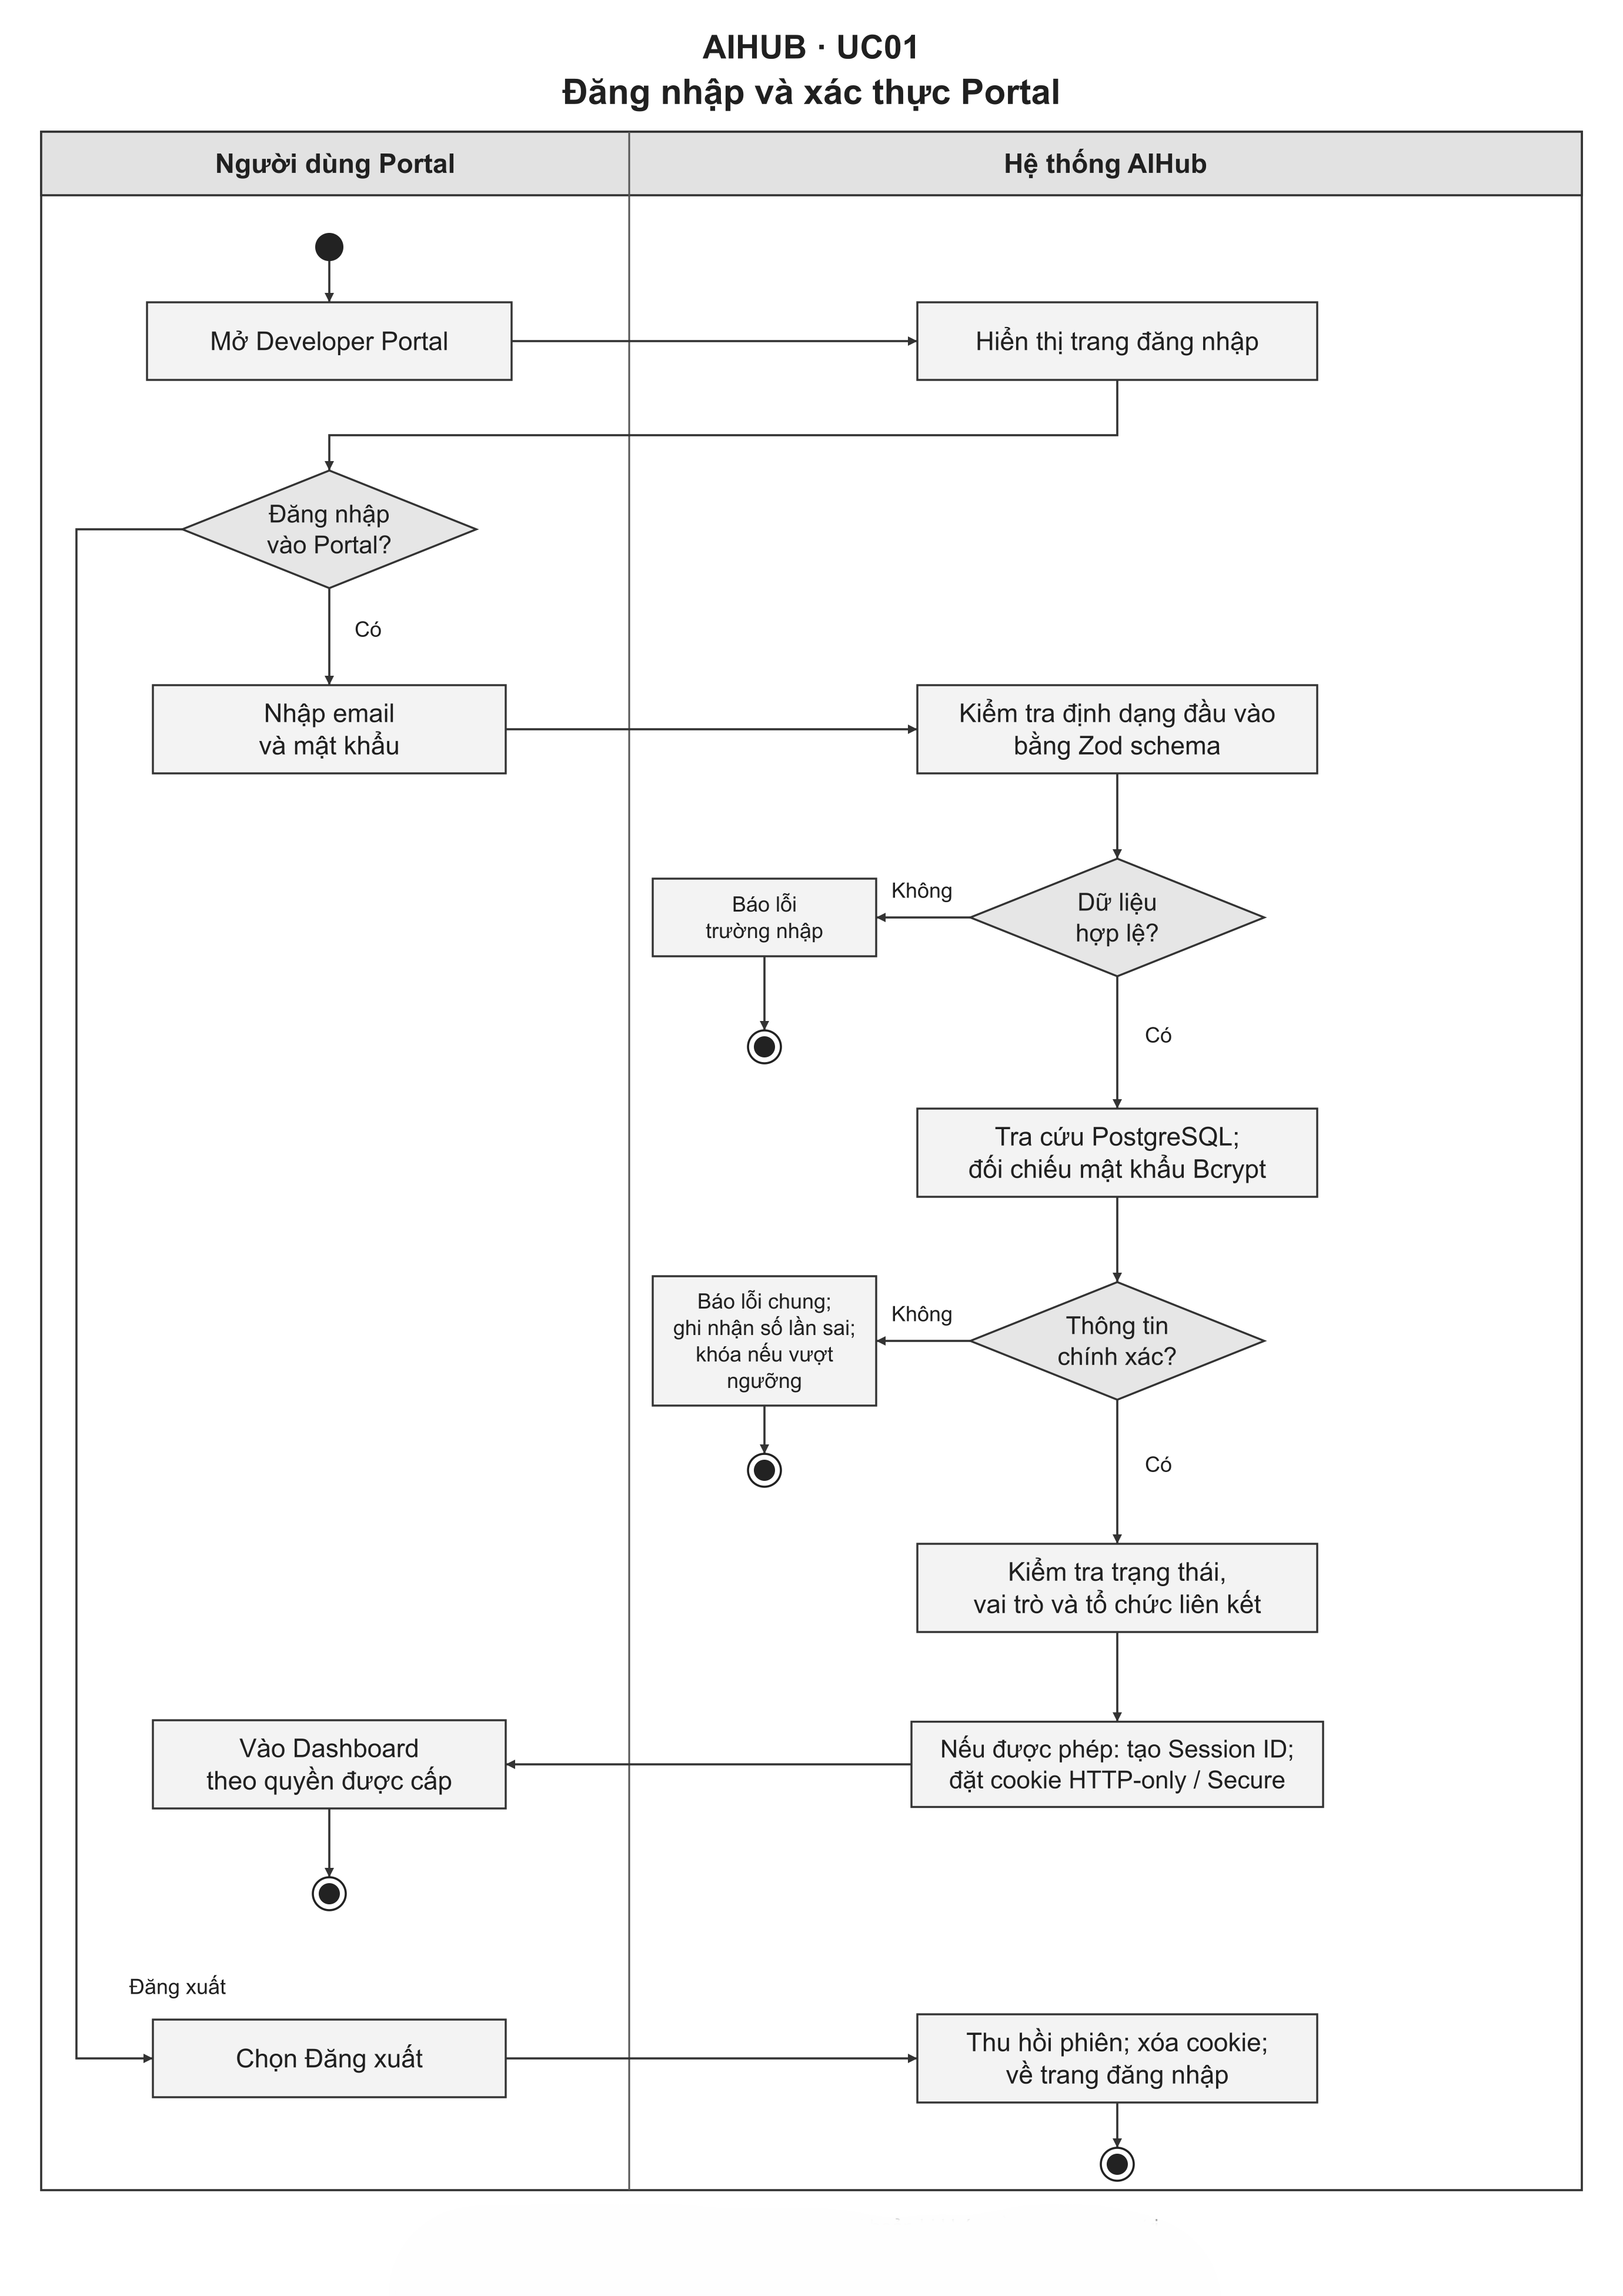
\includegraphics[width=\linewidth,height=0.72\textheight,keepaspectratio]{Images/Activity/AIHub/activity_uc01_portal_auth.png}
    \caption{Sơ đồ hoạt động AIHub -- Use-case 1: Đăng nhập và xác thực Portal}
    \label{aihub:fig:activity_uc01}
    \label{aihub:fig:act_uc1_dev_auth}
\end{figure}

Người dùng mở Portal và nhập thông tin đăng nhập. Khi đăng xuất, hệ thống thu hồi phiên và trở về trang đăng nhập.
% activity-generated:end


\clearpage

\paragraph{Luồng hoạt động: Quản lý khóa API (Use-case 2)}

% activity-generated:start
\begin{figure}[H]
    \centering
    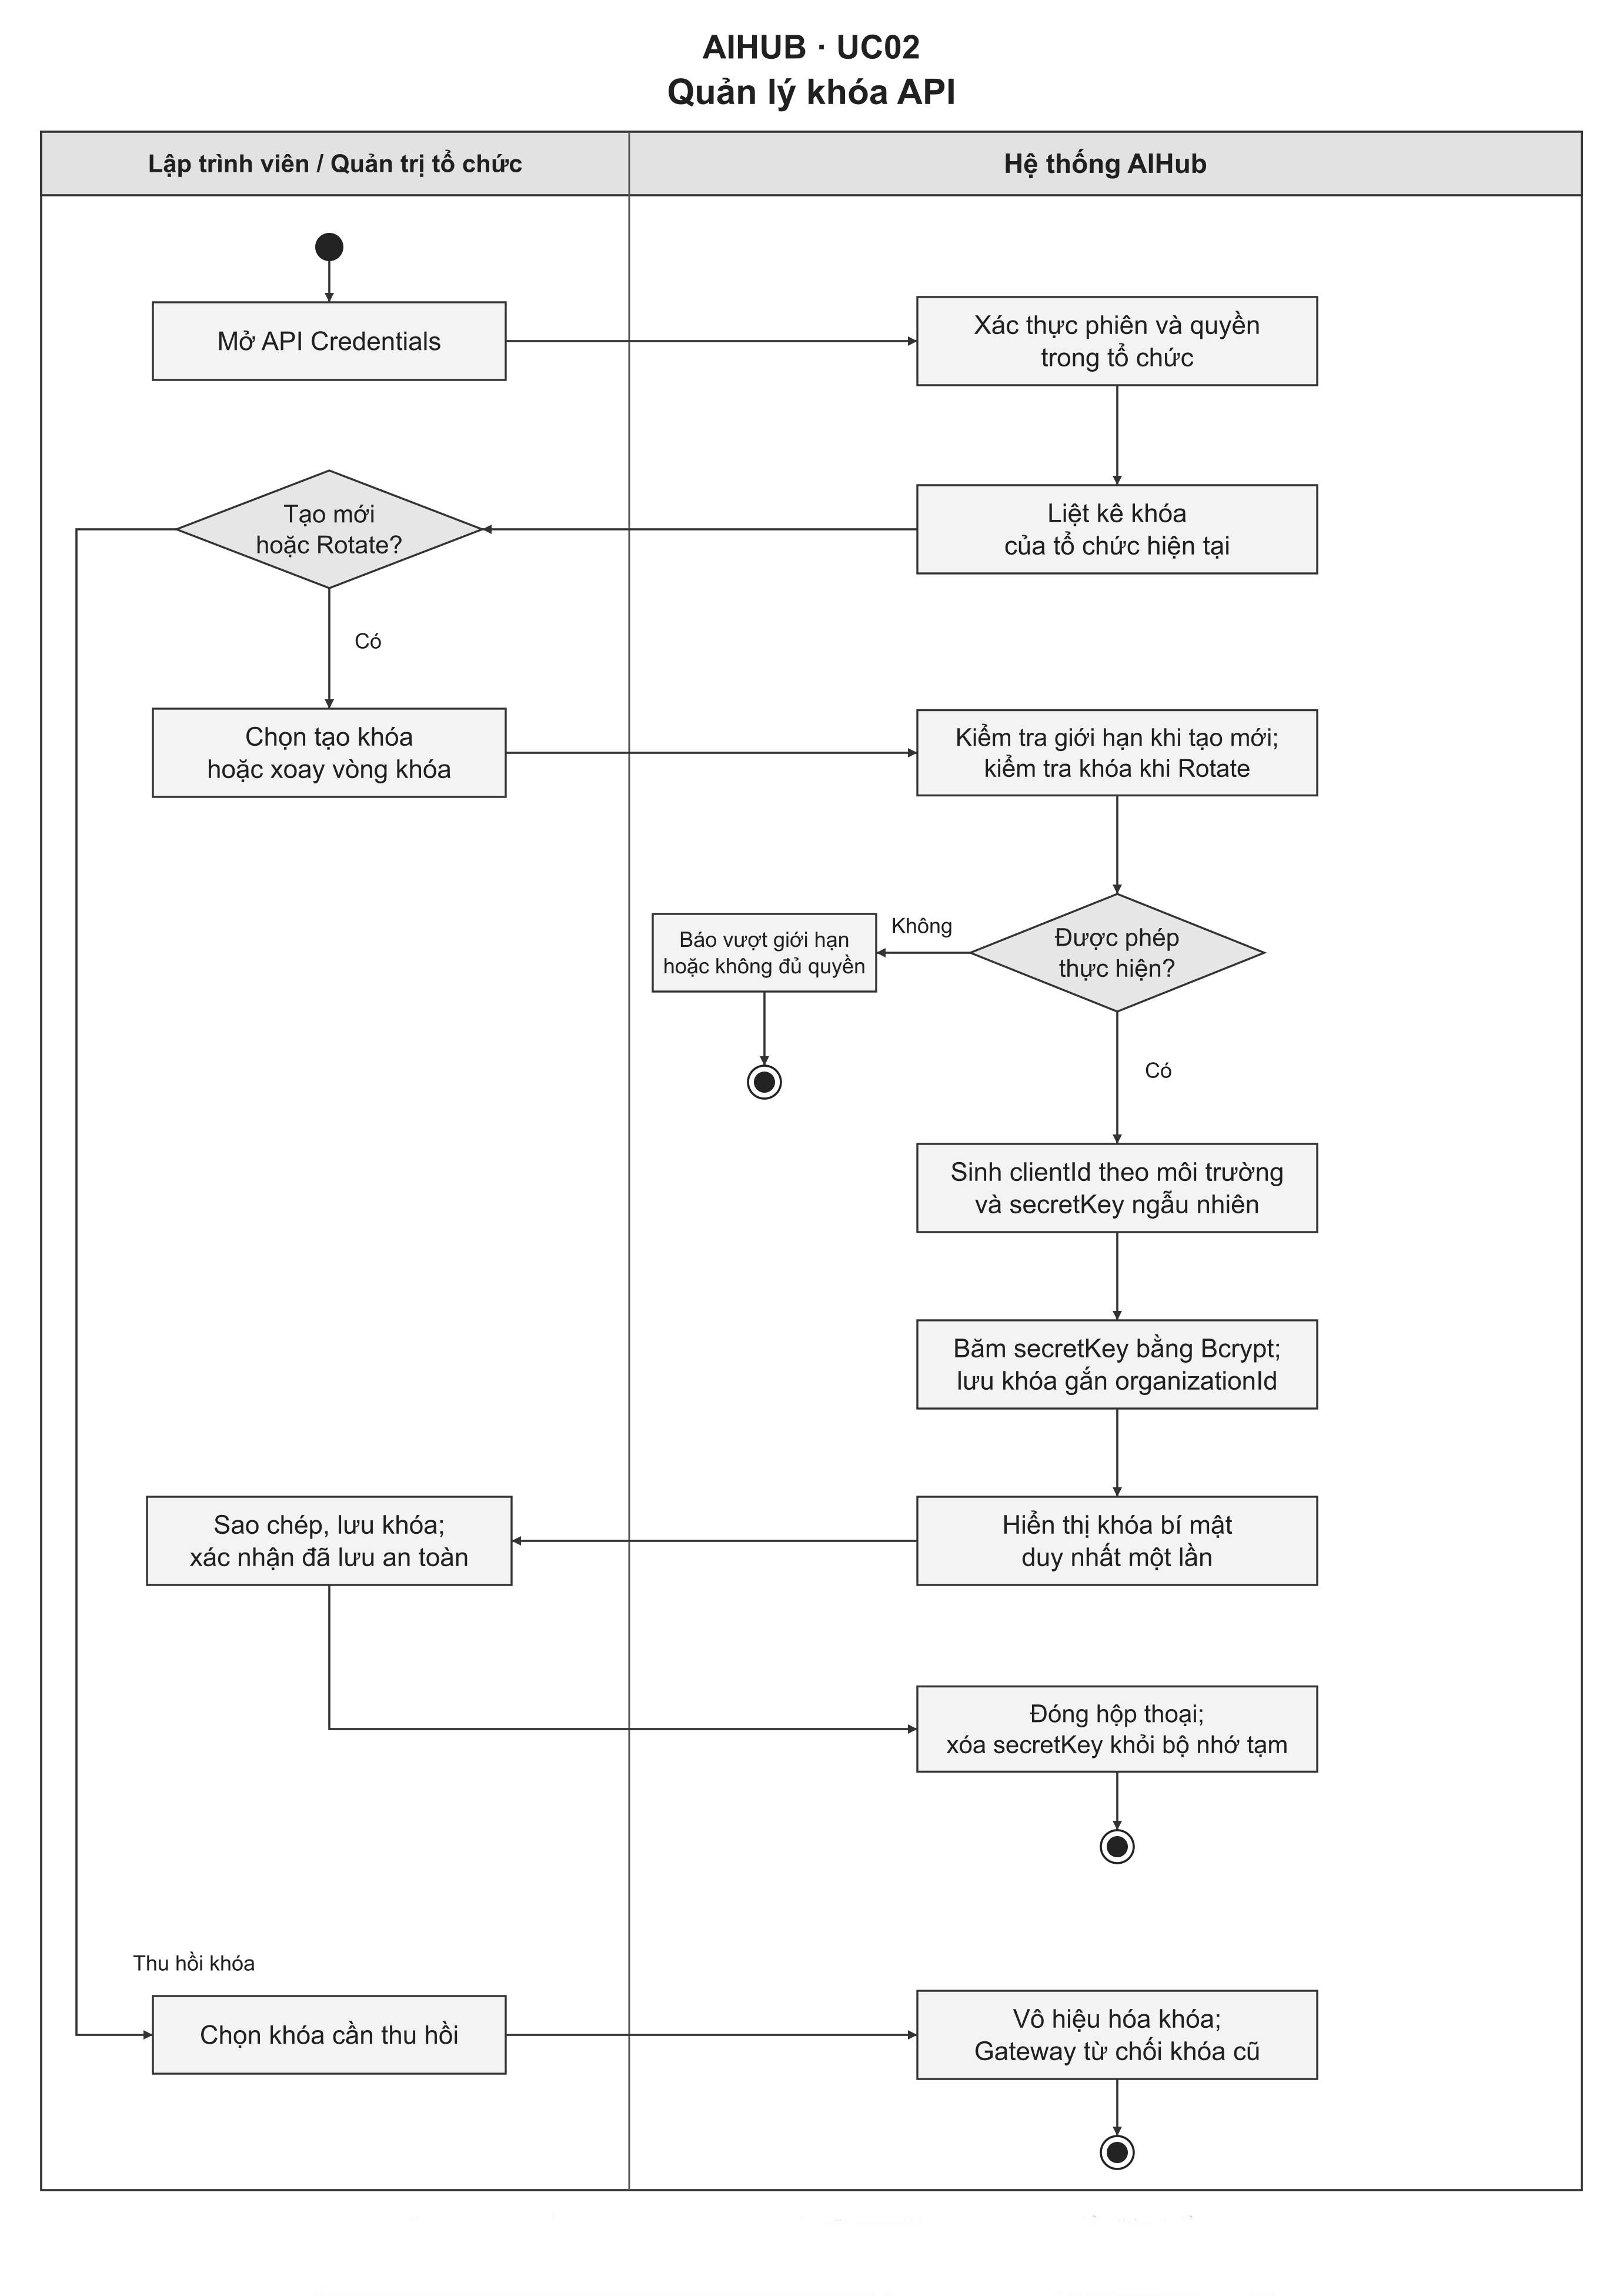
\includegraphics[width=\linewidth,height=0.72\textheight,keepaspectratio]{Images/Activity/AIHub/activity_uc02_api_credentials.png}
    \caption{Sơ đồ hoạt động AIHub -- Use-case 2: Quản lý khóa API}
    \label{aihub:fig:activity_uc02}
    \label{aihub:fig:act_uc2_manage_credentials}
\end{figure}

Người dùng mở danh sách khóa API và chọn tạo mới, xoay vòng hoặc thu hồi. Khóa bị thu hồi không còn được Gateway chấp nhận.
% activity-generated:end


\clearpage

\paragraph{Luồng hoạt động: Kiểm thử cURL Sandbox (Use-case 3)}

% activity-generated:start
\begin{figure}[H]
    \centering
    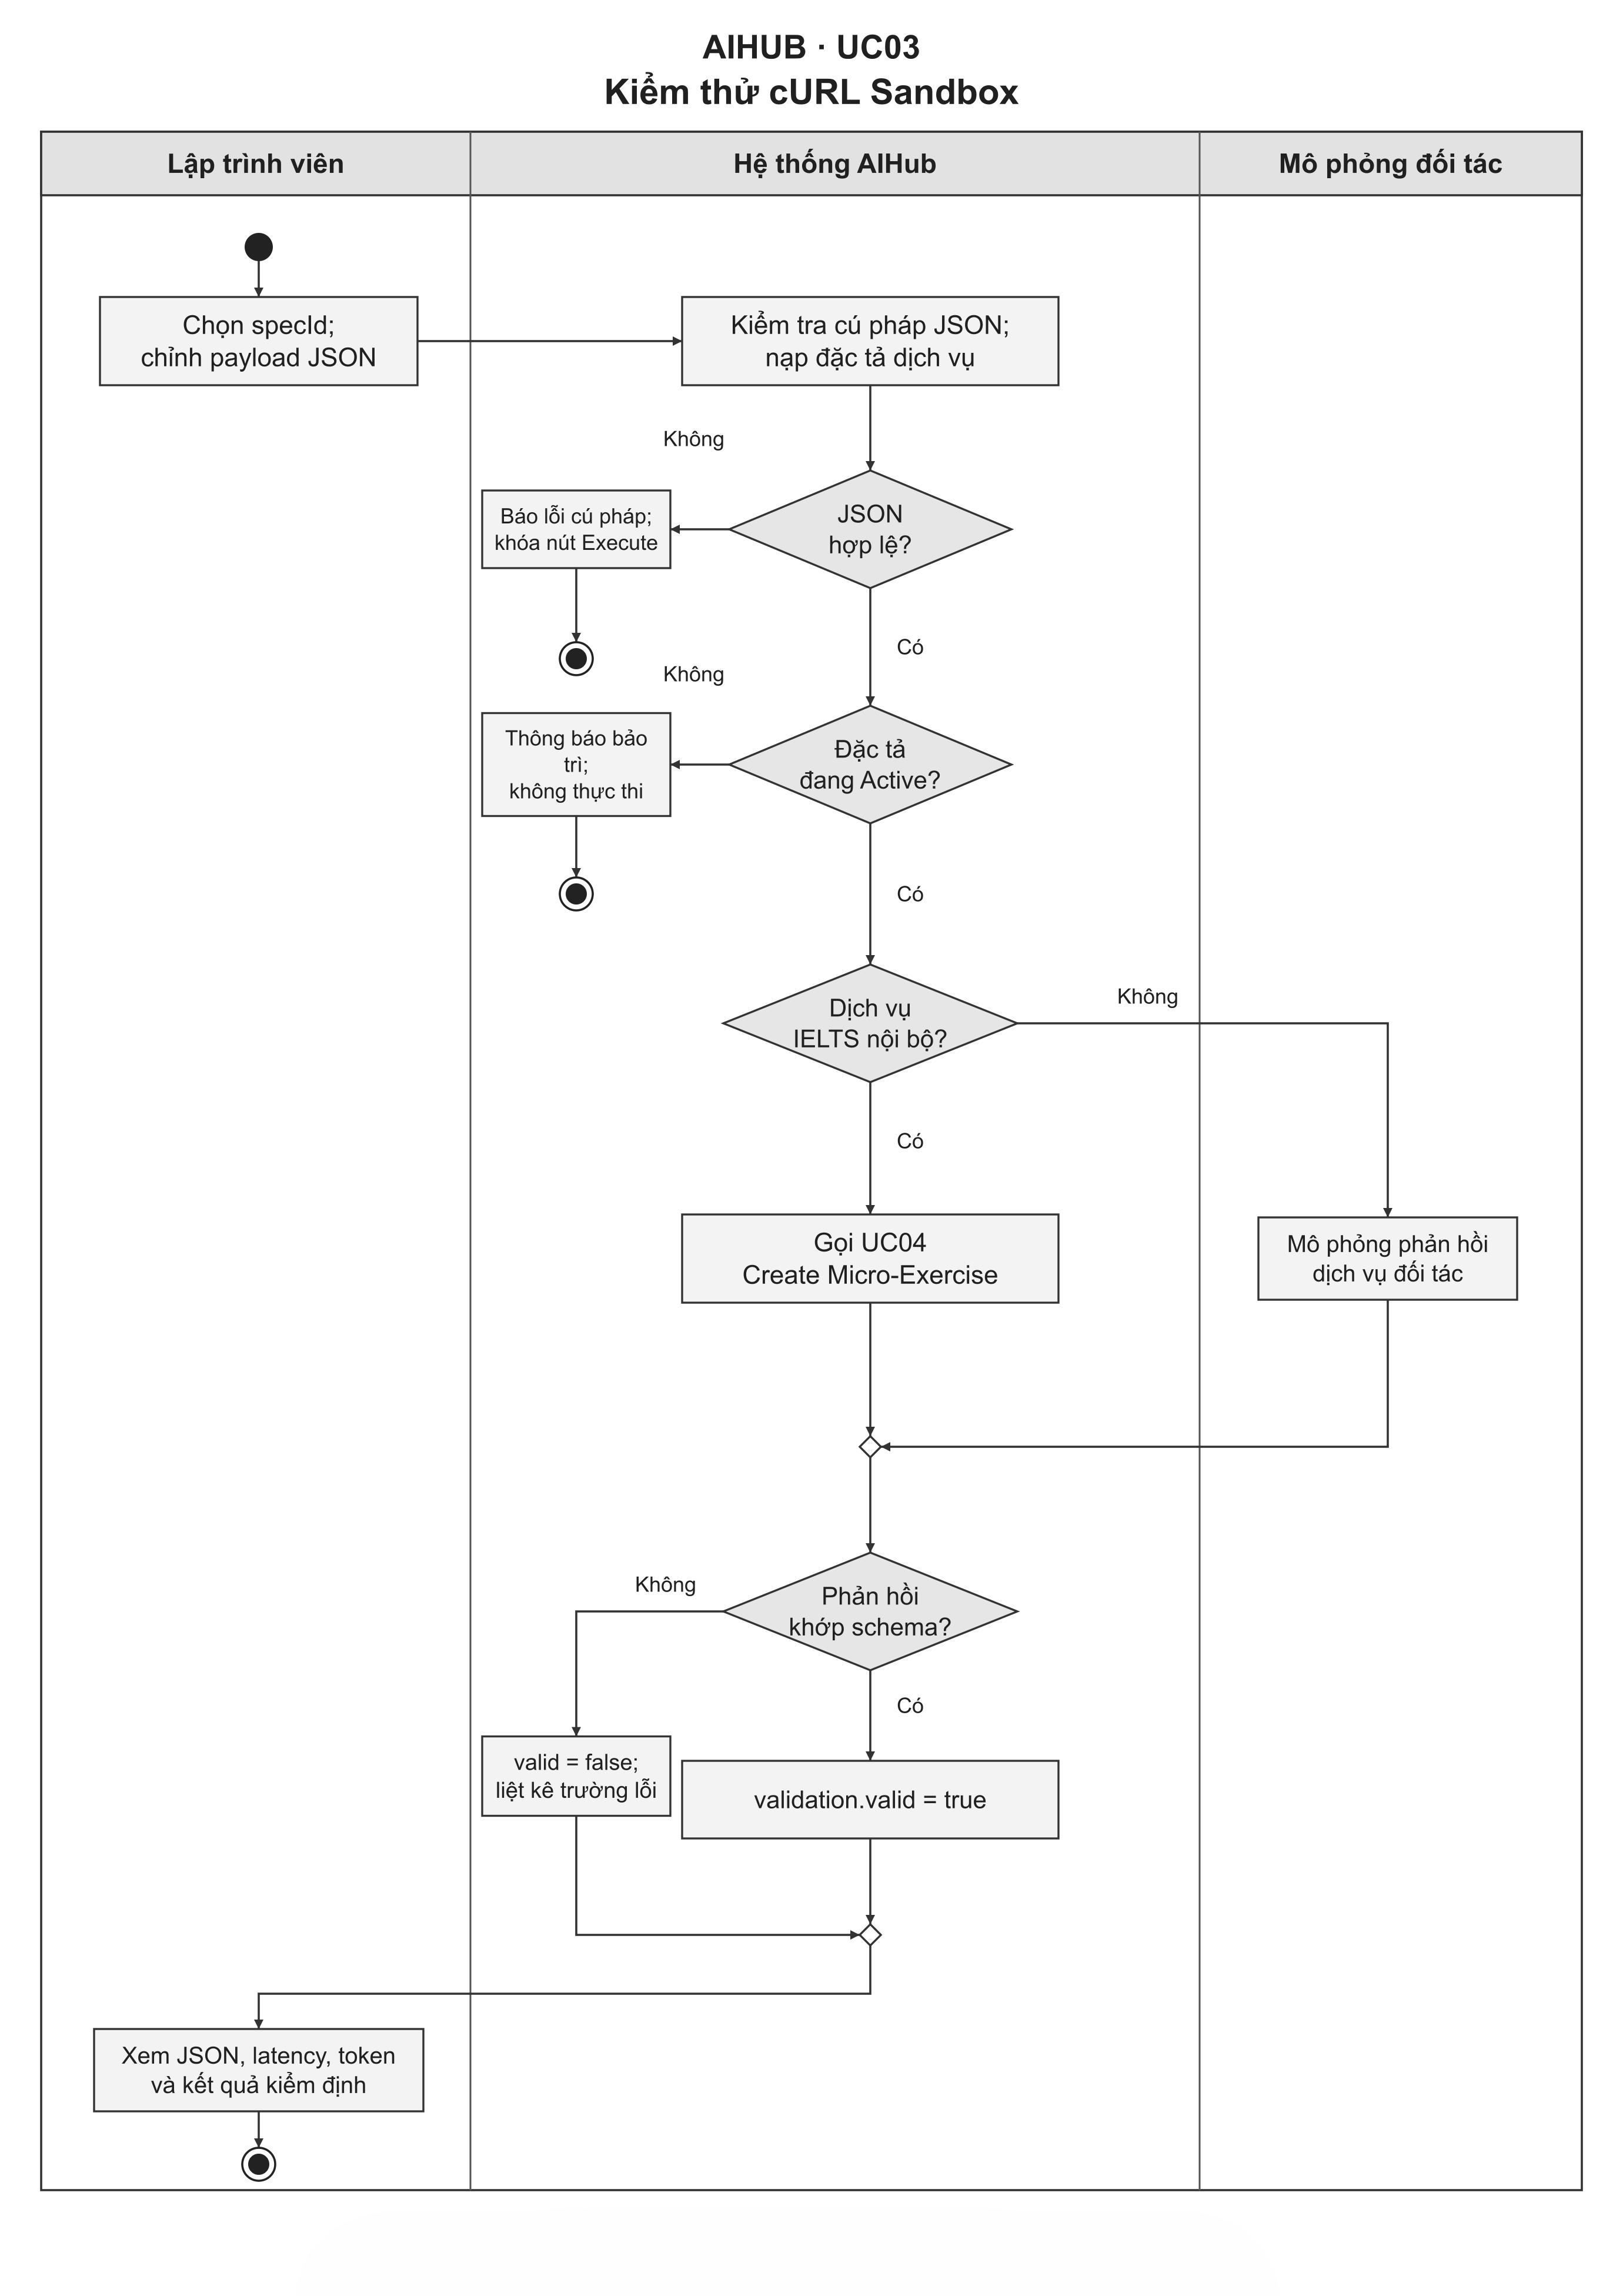
\includegraphics[width=\linewidth,height=0.72\textheight,keepaspectratio]{Images/Activity/AIHub/activity_uc03_curl_sandbox.png}
    \caption{Sơ đồ hoạt động AIHub -- Use-case 3: Kiểm thử cURL Sandbox}
    \label{aihub:fig:activity_uc03}
    \label{aihub:fig:act_uc3_run_spec_curl}
\end{figure}

Lập trình viên chọn đặc tả và nhập dữ liệu thử nghiệm. Sandbox hiển thị kết quả, thời gian xử lý và kết quả kiểm định.
% activity-generated:end


\clearpage

\paragraph{Luồng hoạt động: Gọi API sinh bài tập vi mô (Use-case 4)}

% activity-generated:start
\begin{figure}[H]
    \centering
    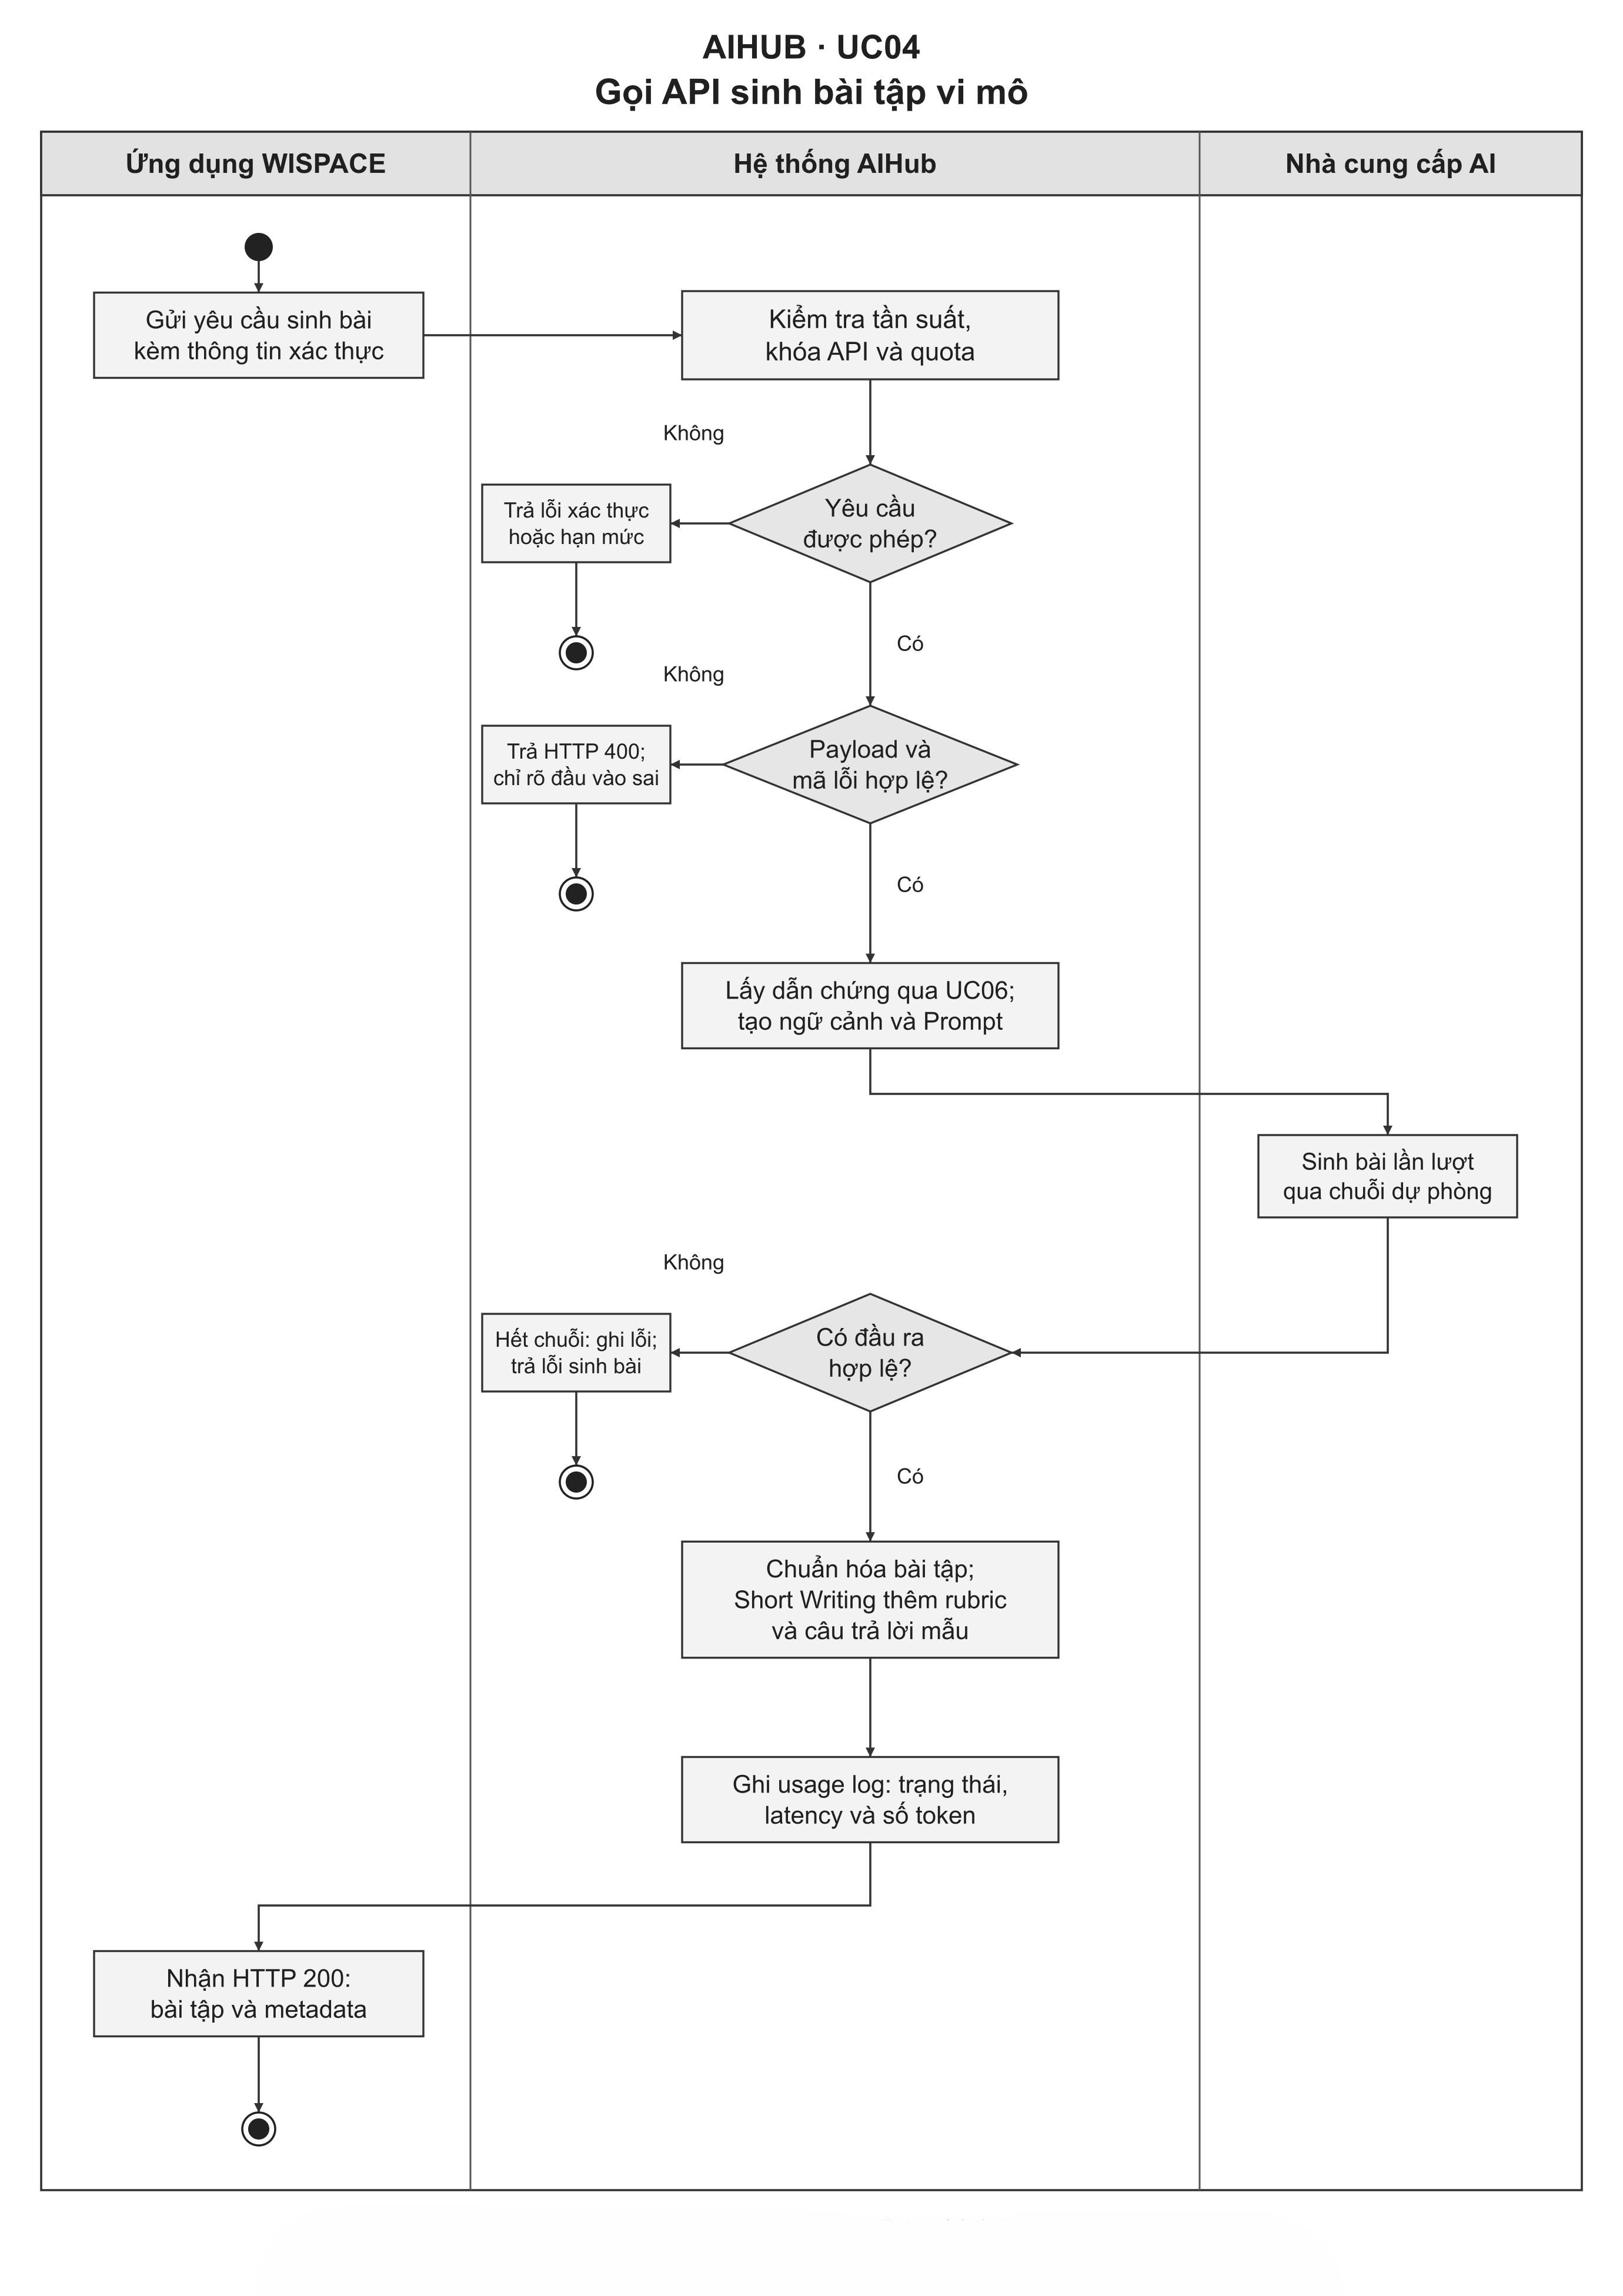
\includegraphics[width=\linewidth,height=0.72\textheight,keepaspectratio]{Images/Activity/AIHub/activity_uc04_create_micro_exercise.png}
    \caption{Sơ đồ hoạt động AIHub -- Use-case 4: Gọi API sinh bài tập vi mô}
    \label{aihub:fig:activity_uc04}
    \label{aihub:fig:act_uc4_create_micro_exercise}
\end{figure}

Ứng dụng gửi yêu cầu sinh bài tập kèm thông tin xác thực. Đầu ra hợp lệ được trả về và ghi nhật ký; nếu không thành công thì trả lỗi.
% activity-generated:end


\clearpage

\paragraph{Luồng hoạt động: Tra cứu hạn mức và Nhật ký sử dụng (Use-case 5)}

% activity-generated:start
\begin{figure}[H]
    \centering
    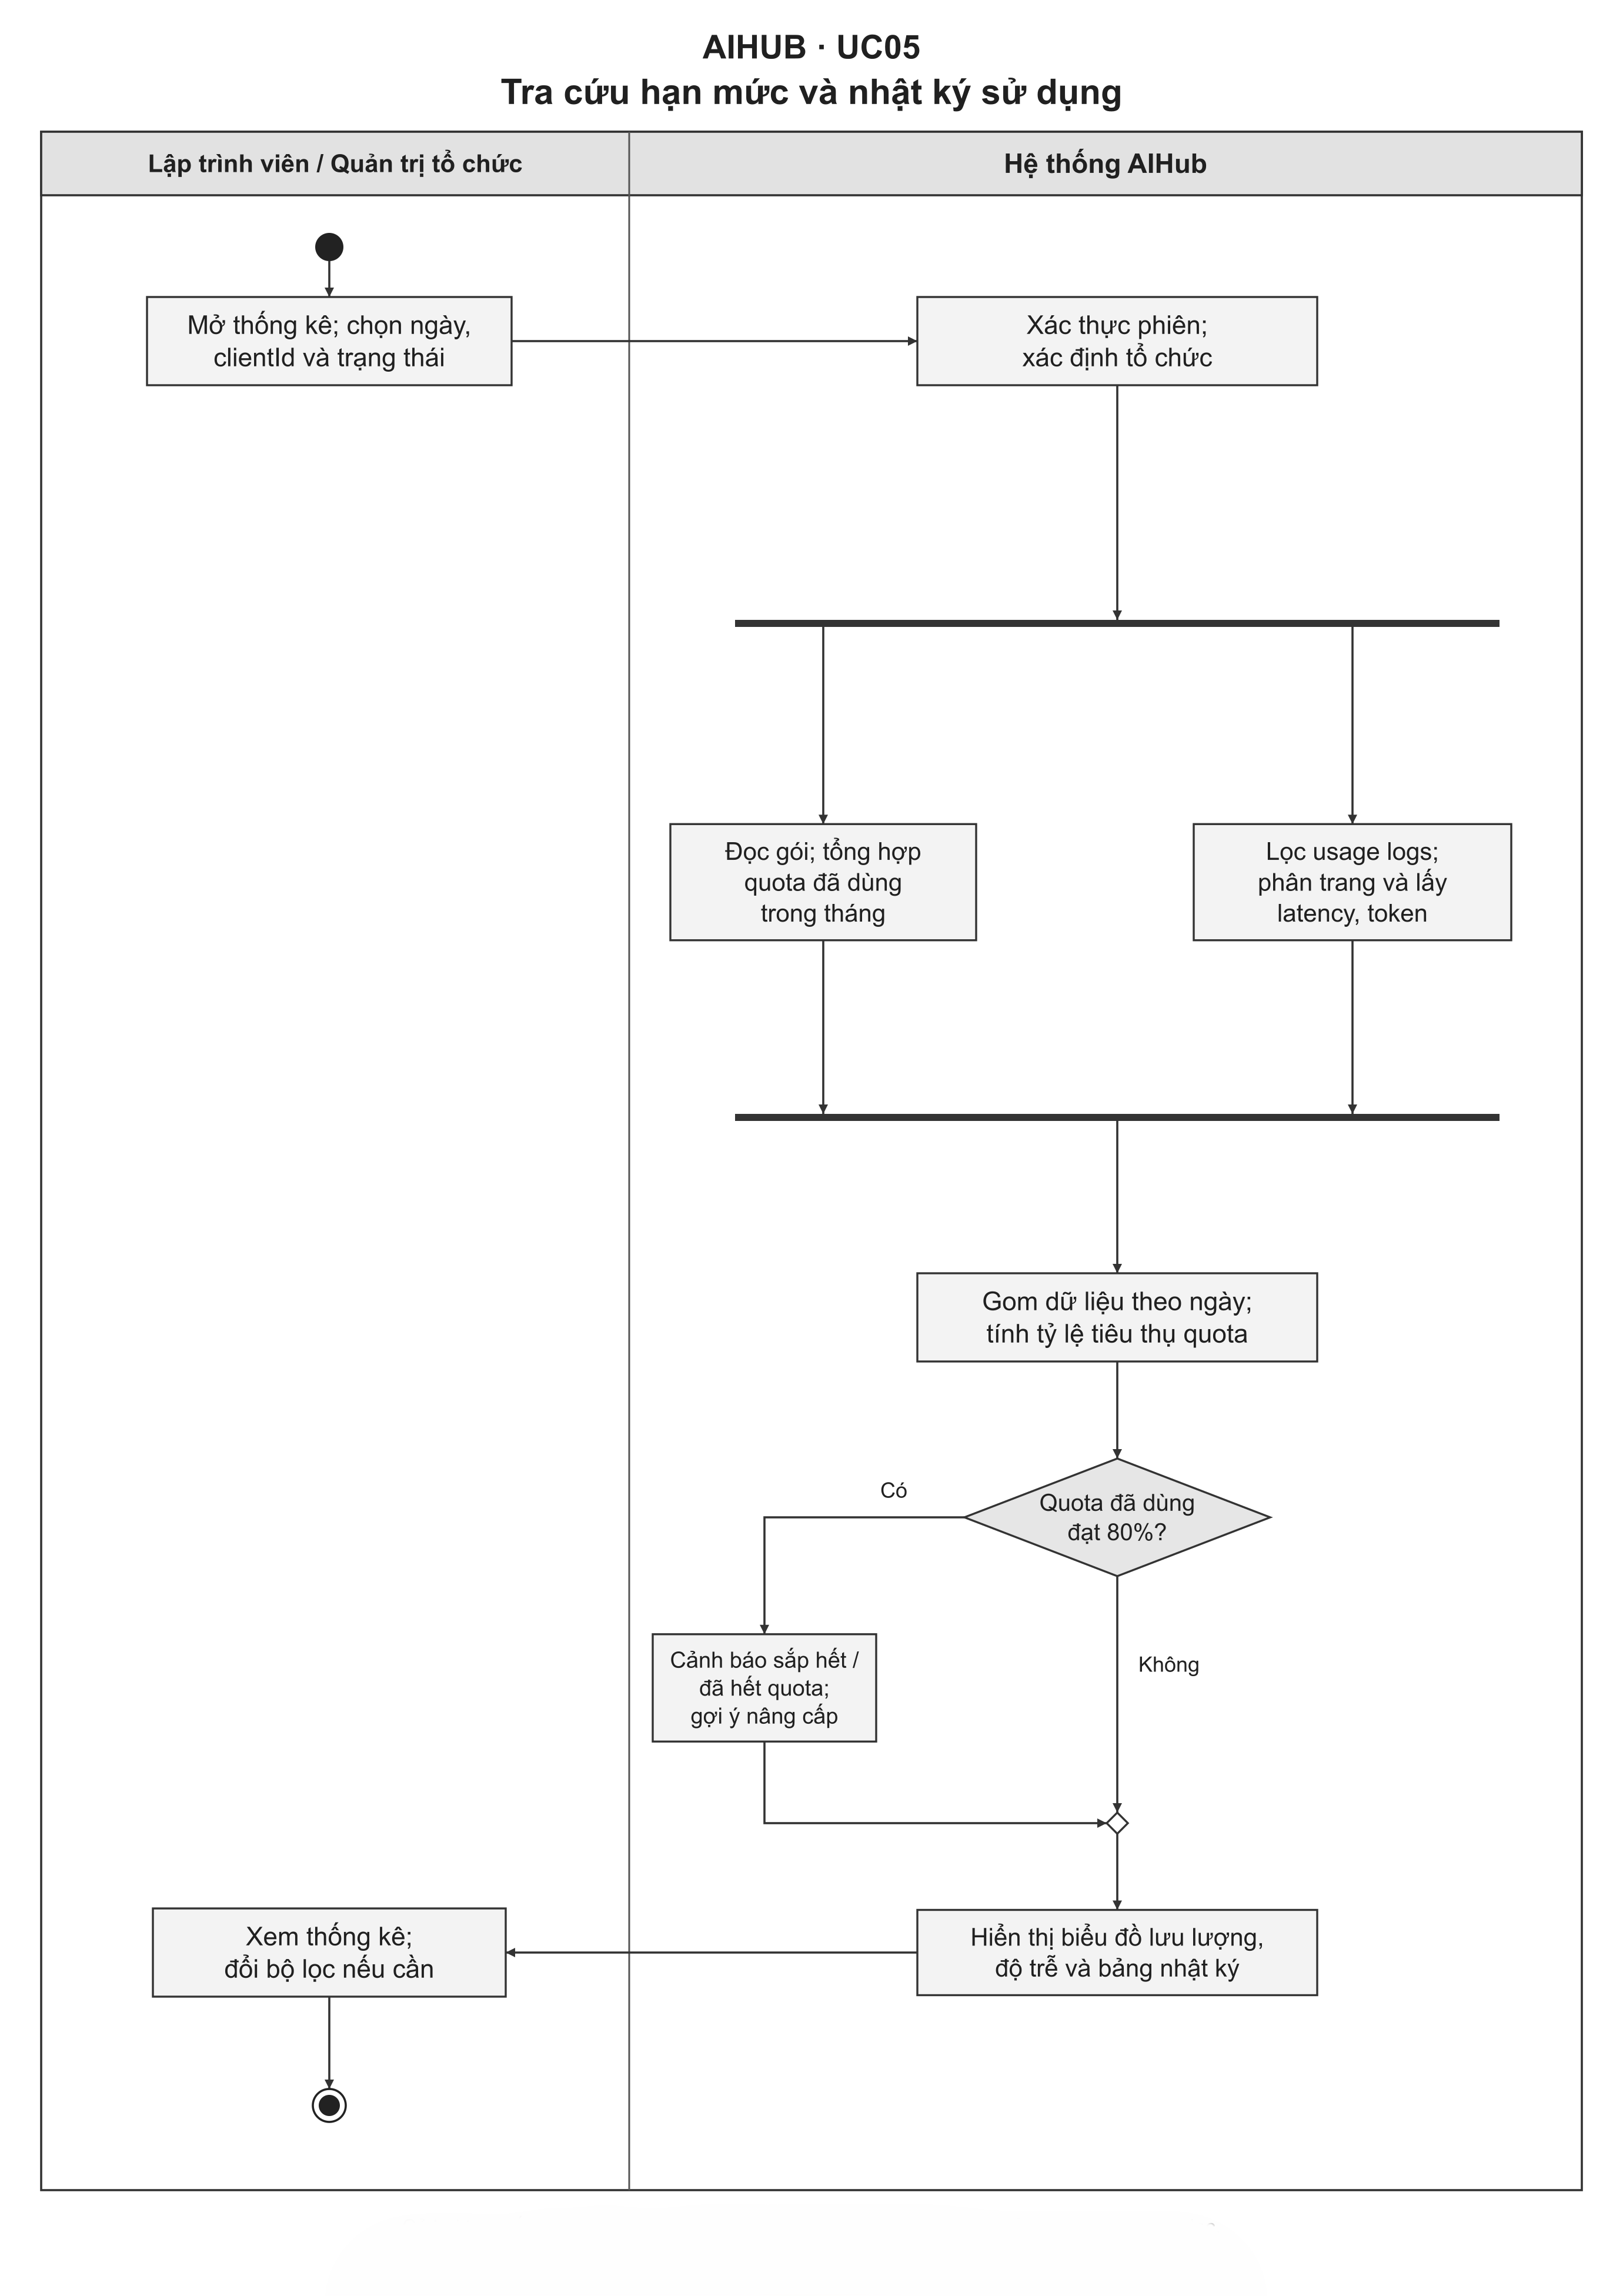
\includegraphics[width=\linewidth,height=0.72\textheight,keepaspectratio]{Images/Activity/AIHub/activity_uc05_quota_usage_logs.png}
    \caption{Sơ đồ hoạt động AIHub -- Use-case 5: Tra cứu hạn mức và nhật ký sử dụng}
    \label{aihub:fig:activity_uc05}
    \label{aihub:fig:act_uc5_view_usage_logs}
\end{figure}

Người dùng chọn khoảng thời gian và điều kiện tra cứu. Kết quả được tổng hợp để hiển thị, xem chi tiết hoặc xuất dữ liệu.
% activity-generated:end


% =========================================================================
% NHÓM 2: CHUYÊN VIÊN HỌC THUẬT (USE-CASE 6 - 11)
% =========================================================================

\clearpage

\paragraph{Luồng hoạt động: Truy vấn ngân hàng lỗi thực tế (Use-case 6)}

% activity-generated:start
\begin{figure}[H]
    \centering
    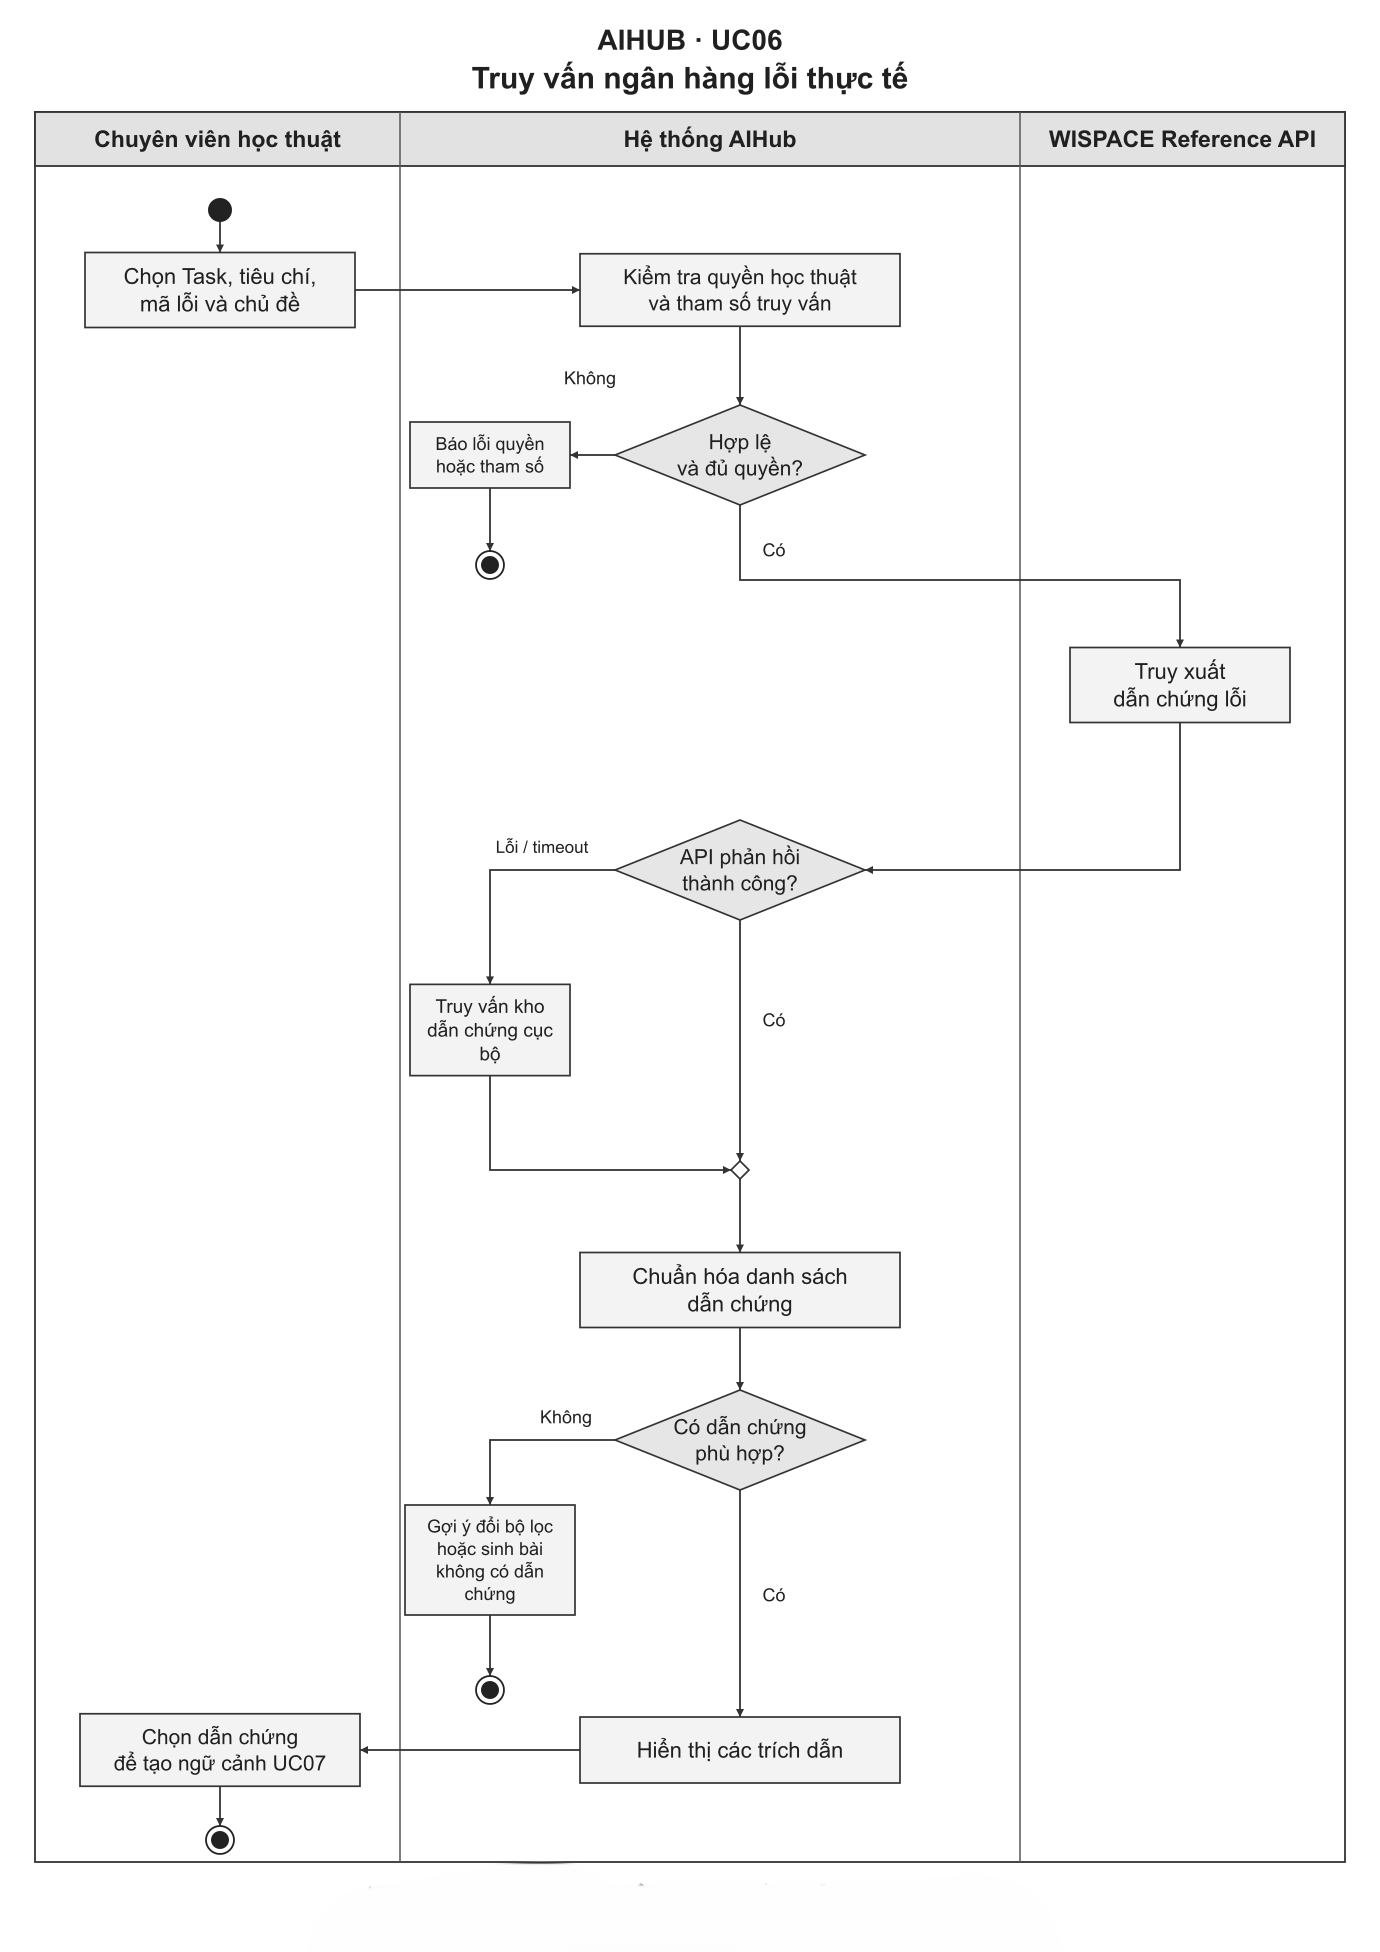
\includegraphics[width=\linewidth,height=0.72\textheight,keepaspectratio]{Images/Activity/AIHub/activity_uc06_essay_references.png}
    \caption{Sơ đồ hoạt động AIHub -- Use-case 6: Truy vấn ngân hàng lỗi thực tế}
    \label{aihub:fig:activity_uc06}
    \label{aihub:fig:act_uc6_query_references}
\end{figure}

Chuyên viên chọn Task, tiêu chí, mã lỗi và chủ đề. Chuyên viên chọn dẫn chứng để tạo ngữ cảnh sinh bài.
% activity-generated:end


\clearpage

\paragraph{Luồng hoạt động: Khởi tạo mẫu bài tập học thuật (Use-case 7)}

% activity-generated:start
\begin{figure}[H]
    \centering
    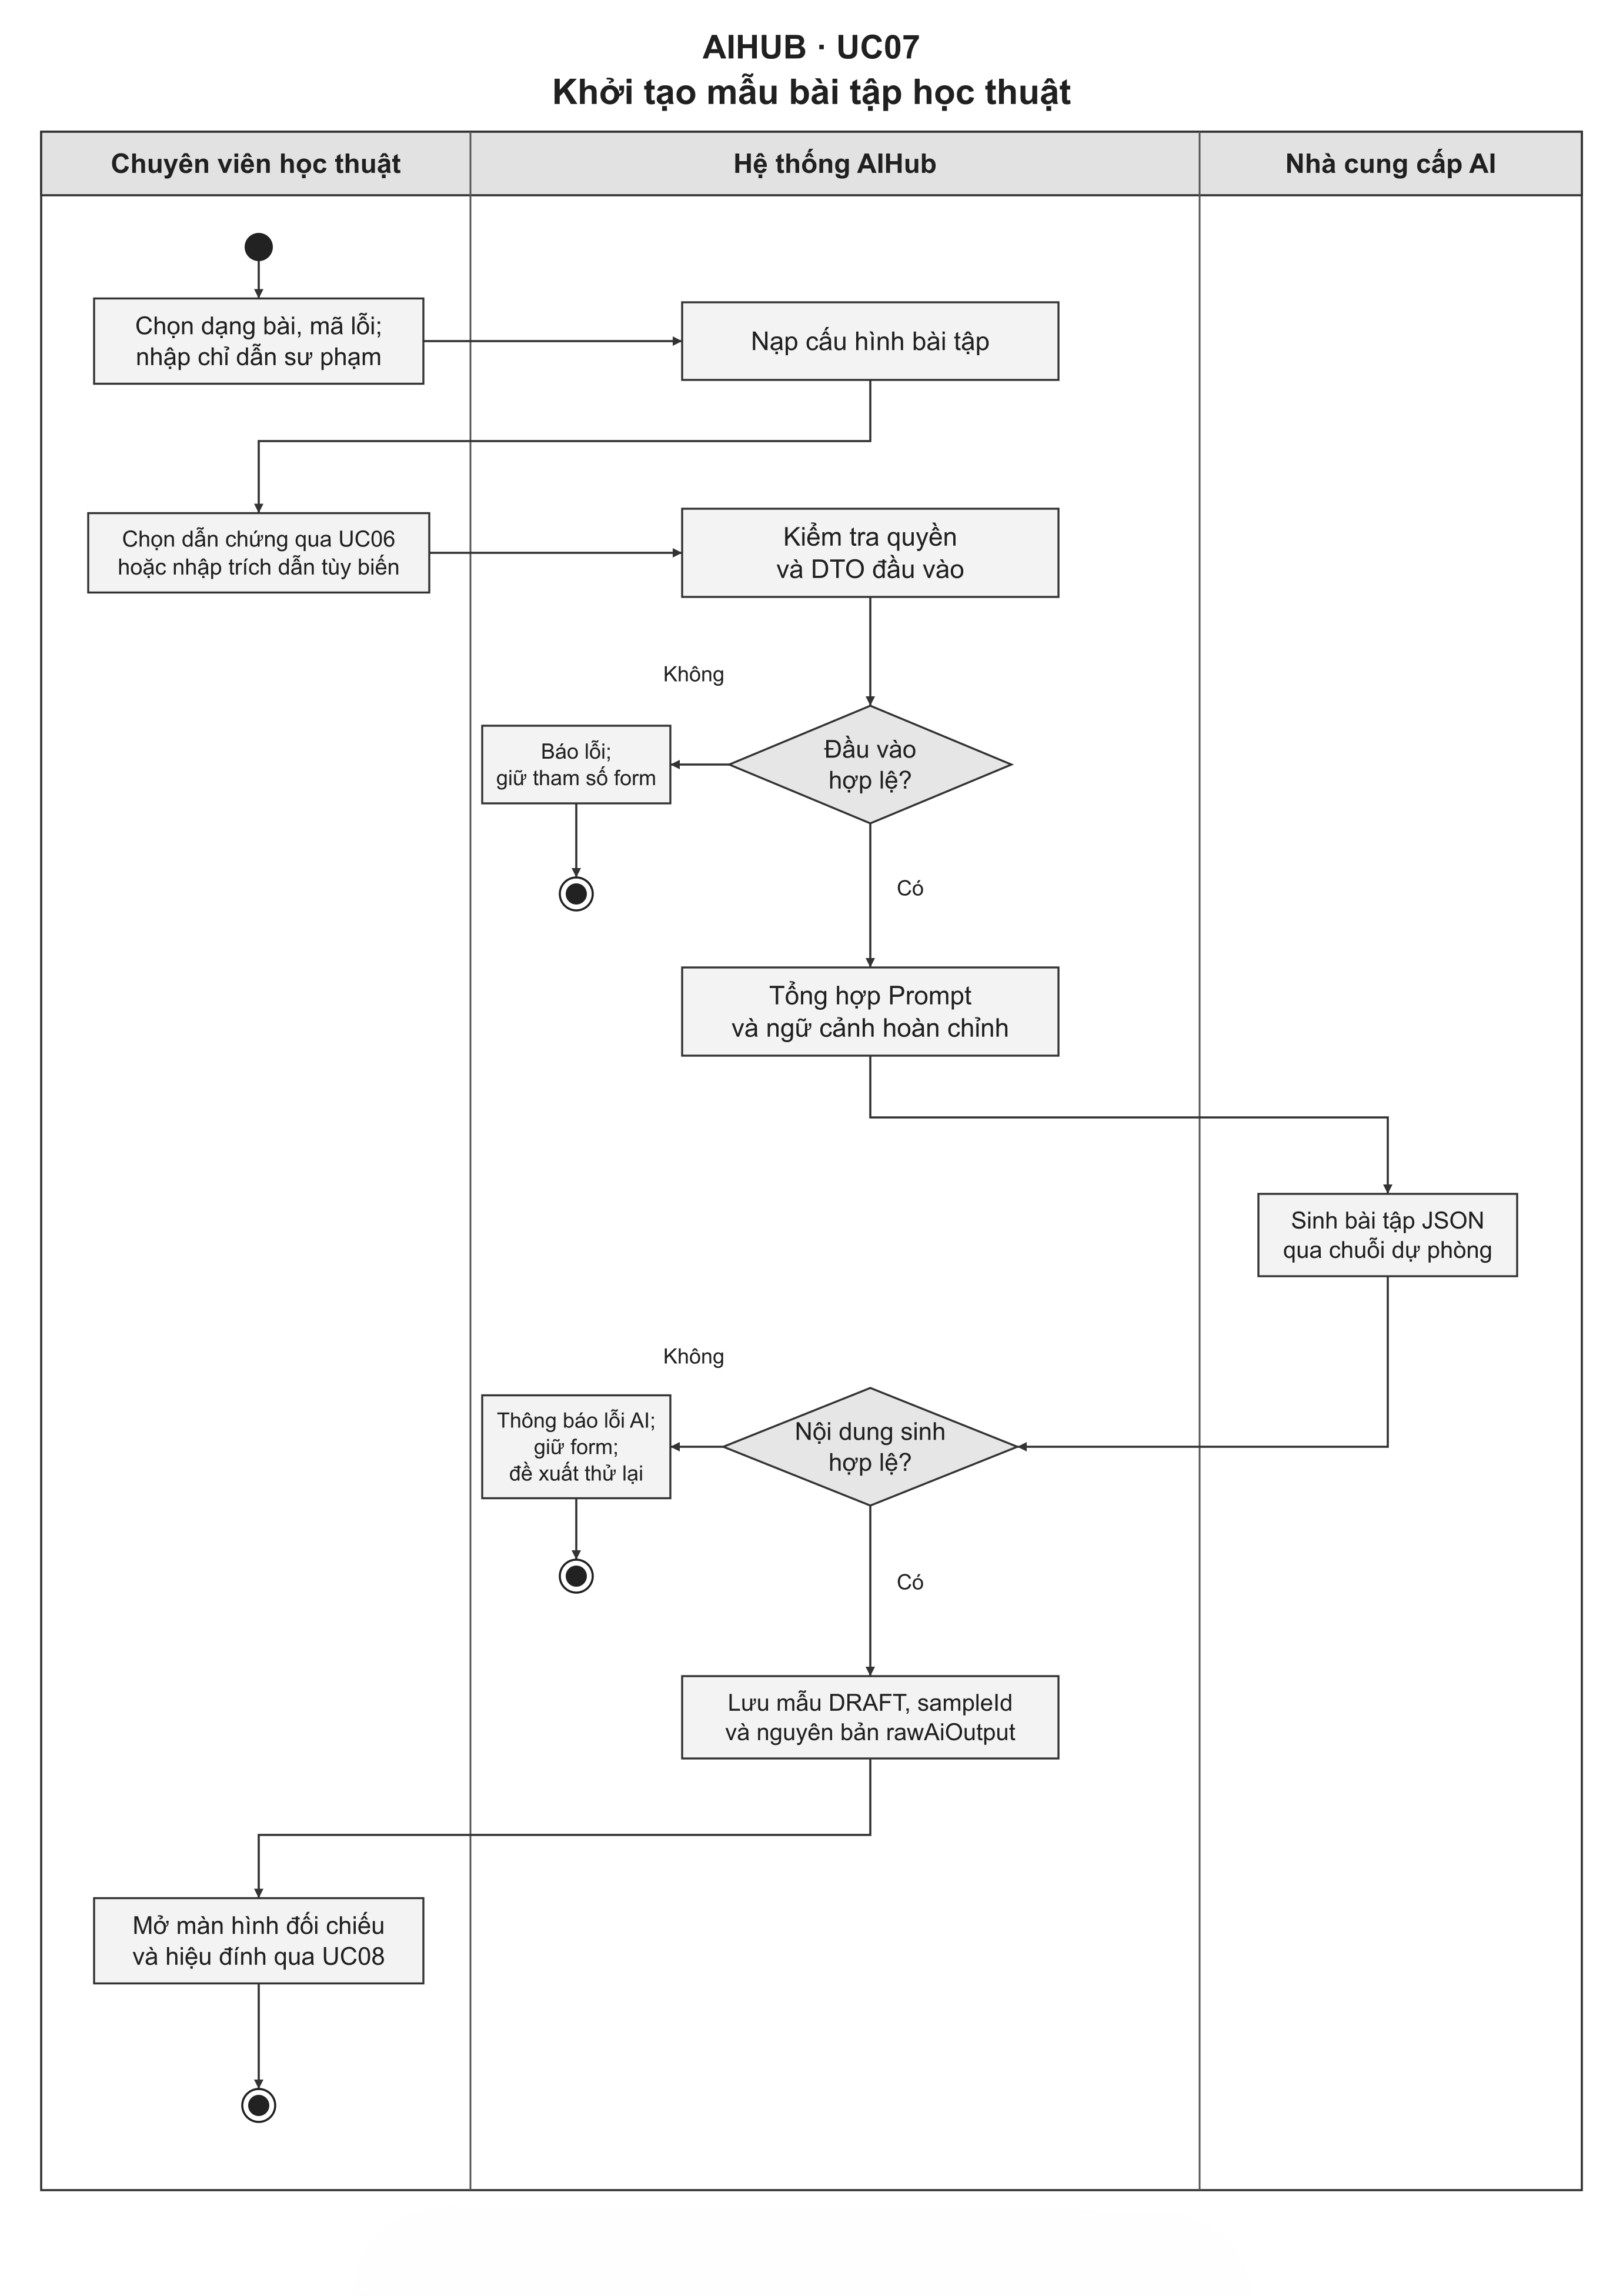
\includegraphics[width=\linewidth,height=0.72\textheight,keepaspectratio]{Images/Activity/AIHub/activity_uc07_generate_academic_sample.png}
    \caption{Sơ đồ hoạt động AIHub -- Use-case 7: Khởi tạo mẫu bài tập học thuật}
    \label{aihub:fig:activity_uc07}
    \label{aihub:fig:act_uc7_academic_generate}
\end{figure}

Chuyên viên chọn yêu cầu bài tập và bổ sung ngữ cảnh hoặc dẫn chứng. Chuyên viên mở mẫu để hiệu đính; nếu sinh lỗi thì có thể thử lại.
% activity-generated:end


\clearpage

\paragraph{Luồng hoạt động: Kiểm định, hiệu đính và chấm điểm bài tập (Use-case 8)}

% activity-generated:start
\begin{figure}[H]
    \centering
    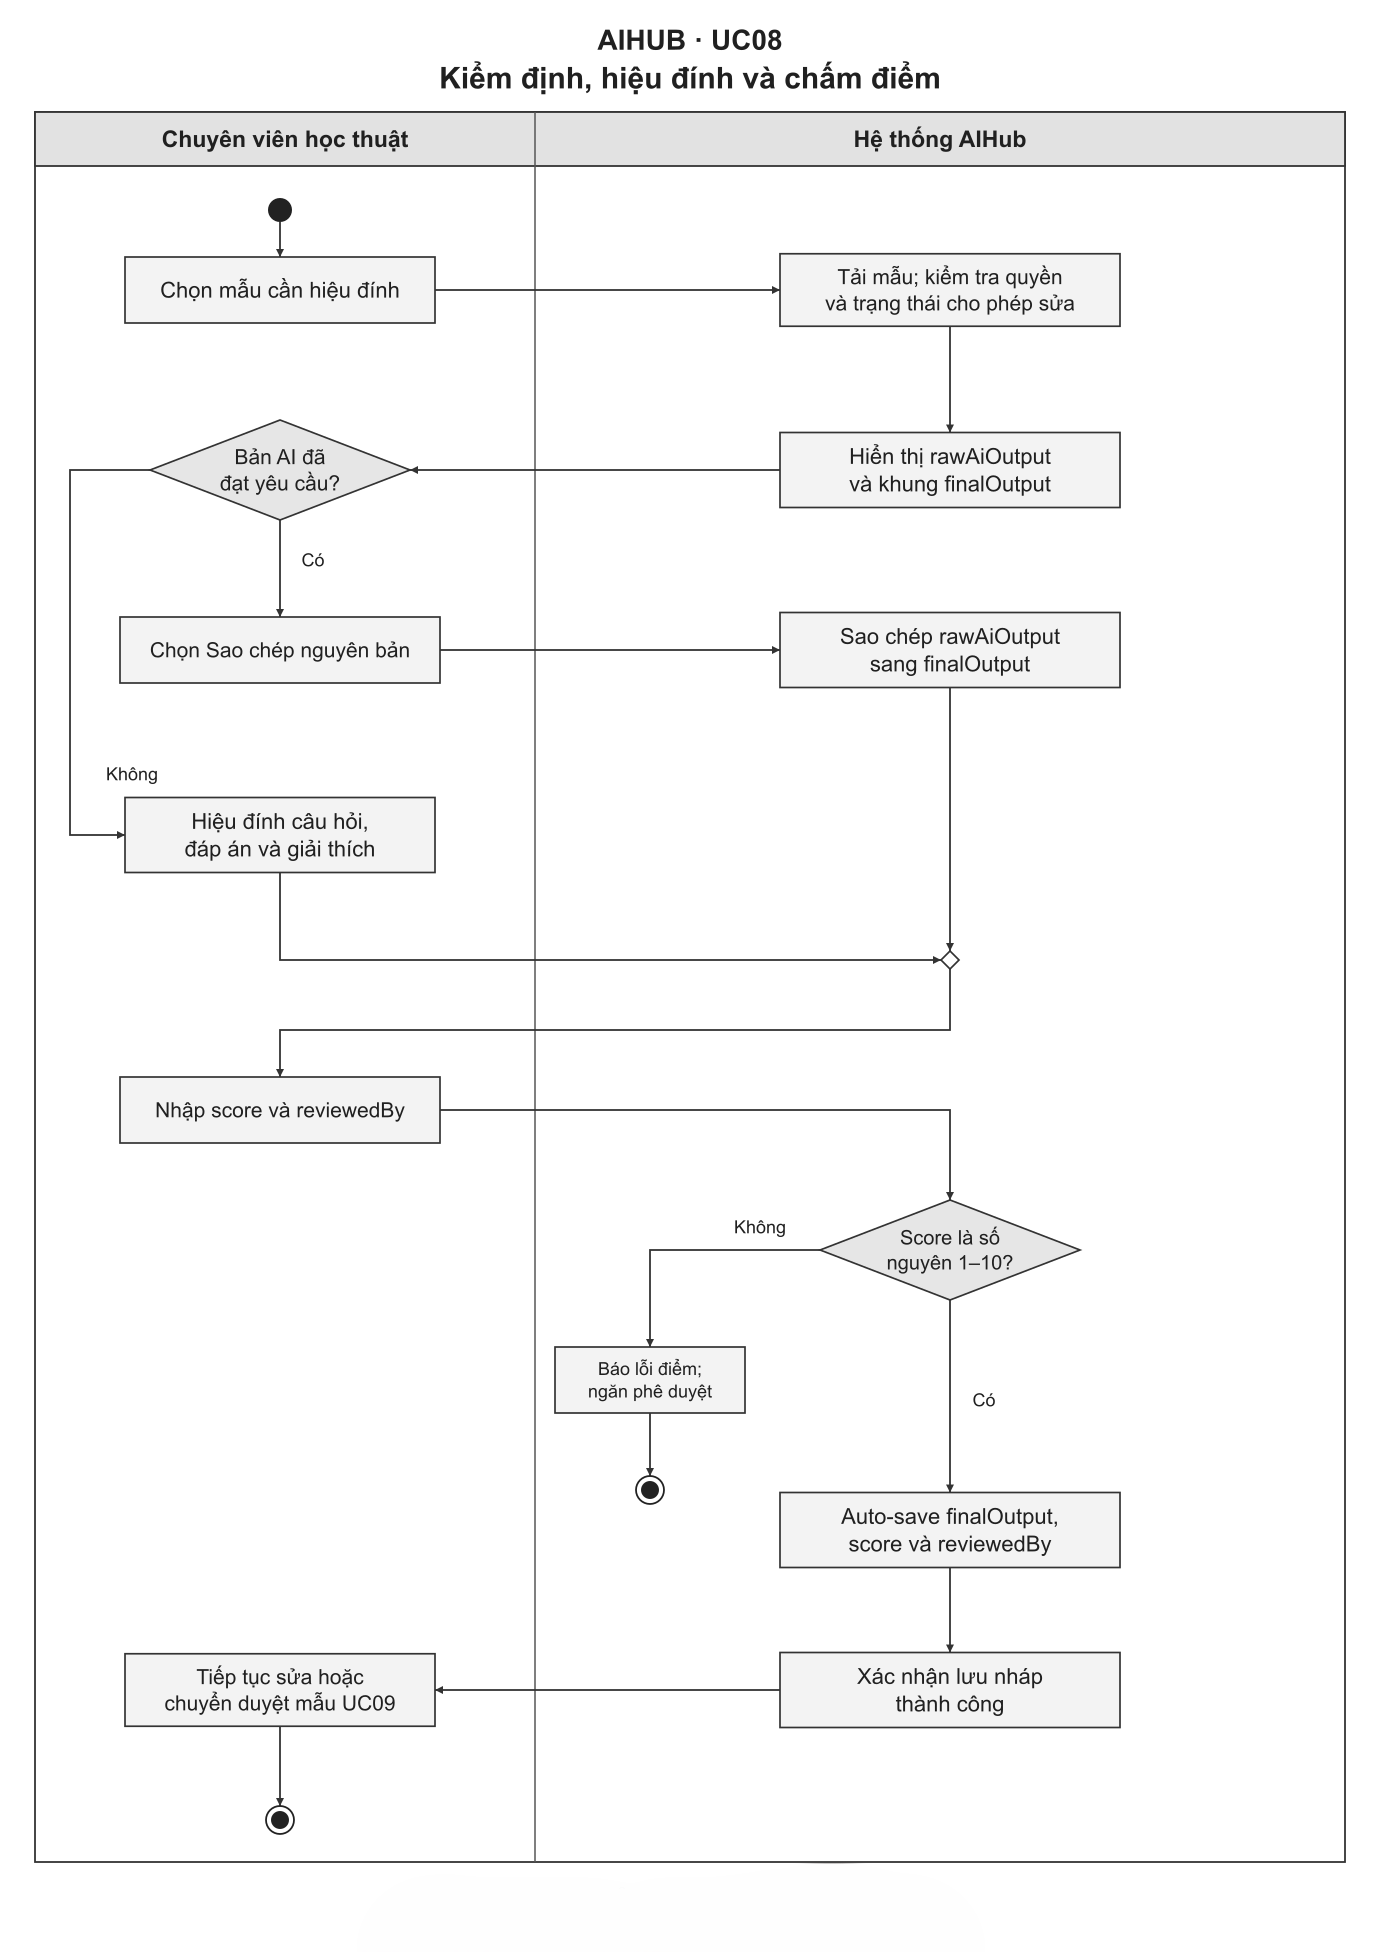
\includegraphics[width=\linewidth,height=0.72\textheight,keepaspectratio]{Images/Activity/AIHub/activity_uc08_review_score_sample.png}
    \caption{Sơ đồ hoạt động AIHub -- Use-case 8: Kiểm định, hiệu đính và chấm điểm}
    \label{aihub:fig:activity_uc08}
    \label{aihub:fig:act_uc8_academic_review_score}
\end{figure}

Chuyên viên mở mẫu và xem nội dung AI đã tạo. Chuyên viên tiếp tục chỉnh sửa hoặc chuyển sang duyệt mẫu.
% activity-generated:end


\clearpage

\paragraph{Luồng hoạt động: Chấp thuận mẫu và xoay vòng lỗi (Use-case 9)}

% activity-generated:start
\begin{figure}[H]
    \centering
    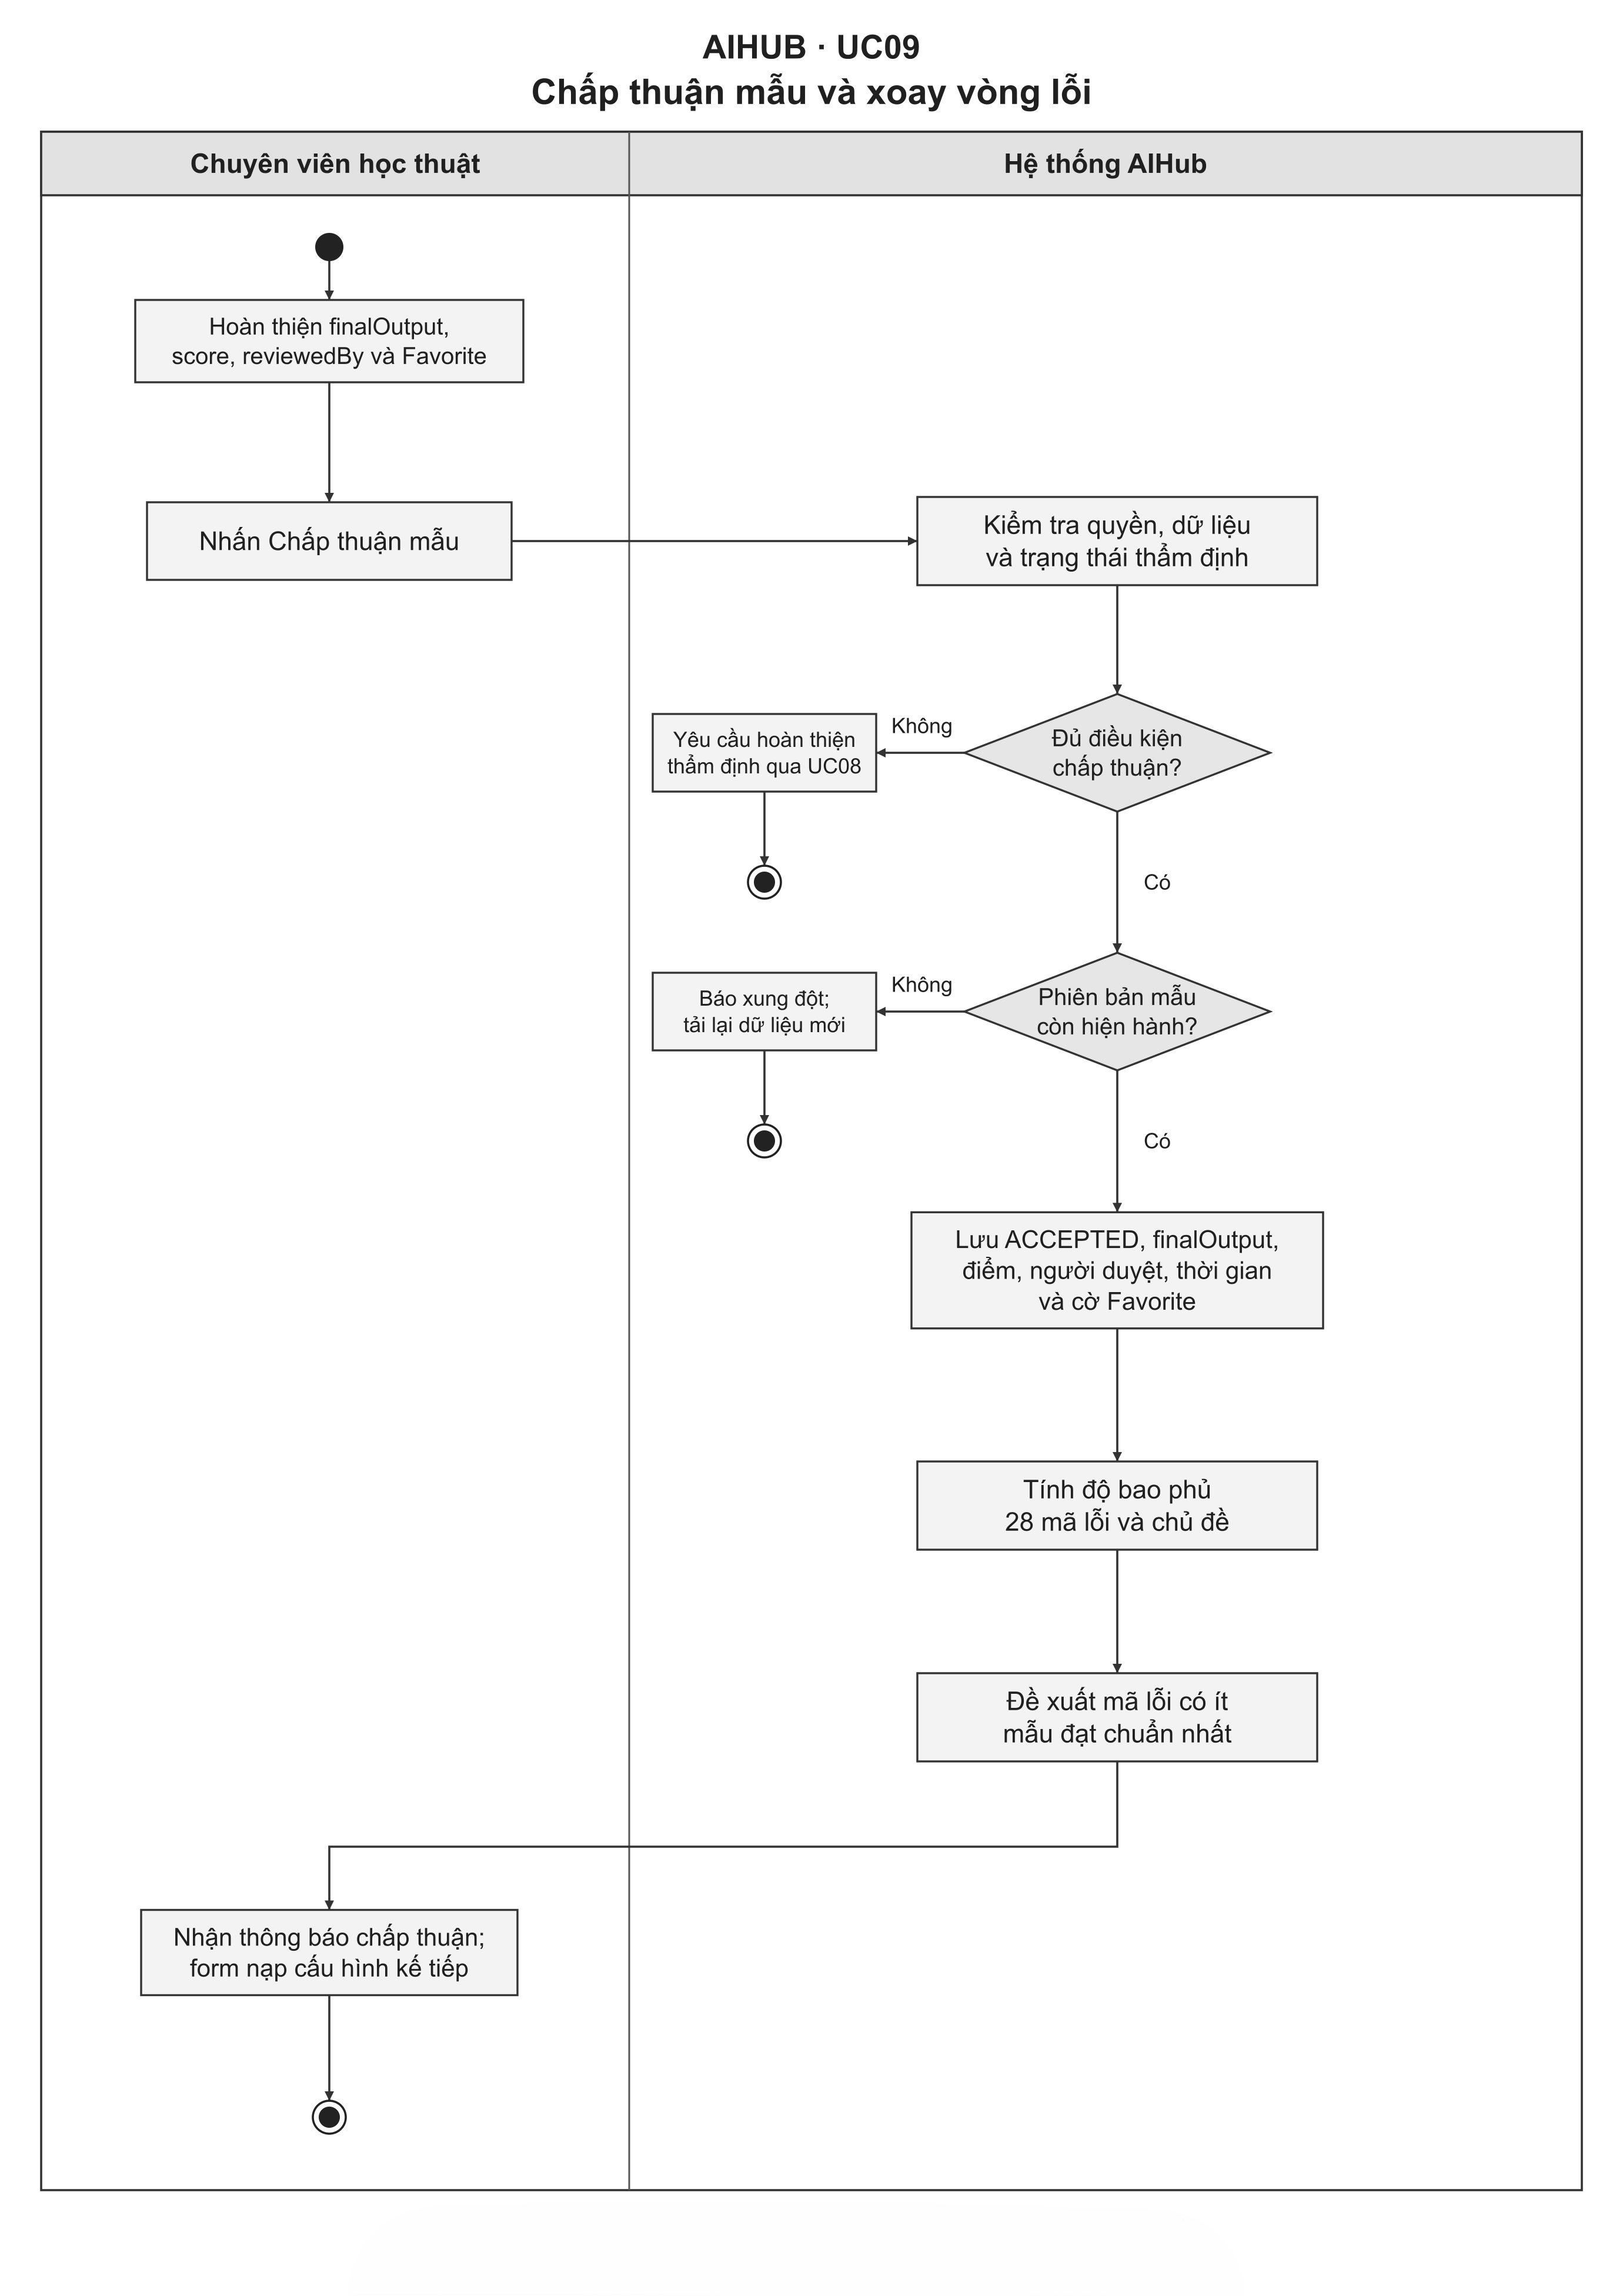
\includegraphics[width=\linewidth,height=0.72\textheight,keepaspectratio]{Images/Activity/AIHub/activity_uc09_accept_sample.png}
    \caption{Sơ đồ hoạt động AIHub -- Use-case 9: Chấp thuận mẫu và xoay vòng lỗi}
    \label{aihub:fig:activity_uc09}
    \label{aihub:fig:act_uc9_academic_accept}
\end{figure}

Chuyên viên kiểm tra mẫu và chọn chấp thuận. Hệ thống cập nhật mức bao phủ lỗi và gợi ý mẫu tiếp theo.
% activity-generated:end


\clearpage

\paragraph{Luồng hoạt động: Từ chối mẫu và thu thập dữ liệu tinh chỉnh (Use-case 10)}

% activity-generated:start
\begin{figure}[H]
    \centering
    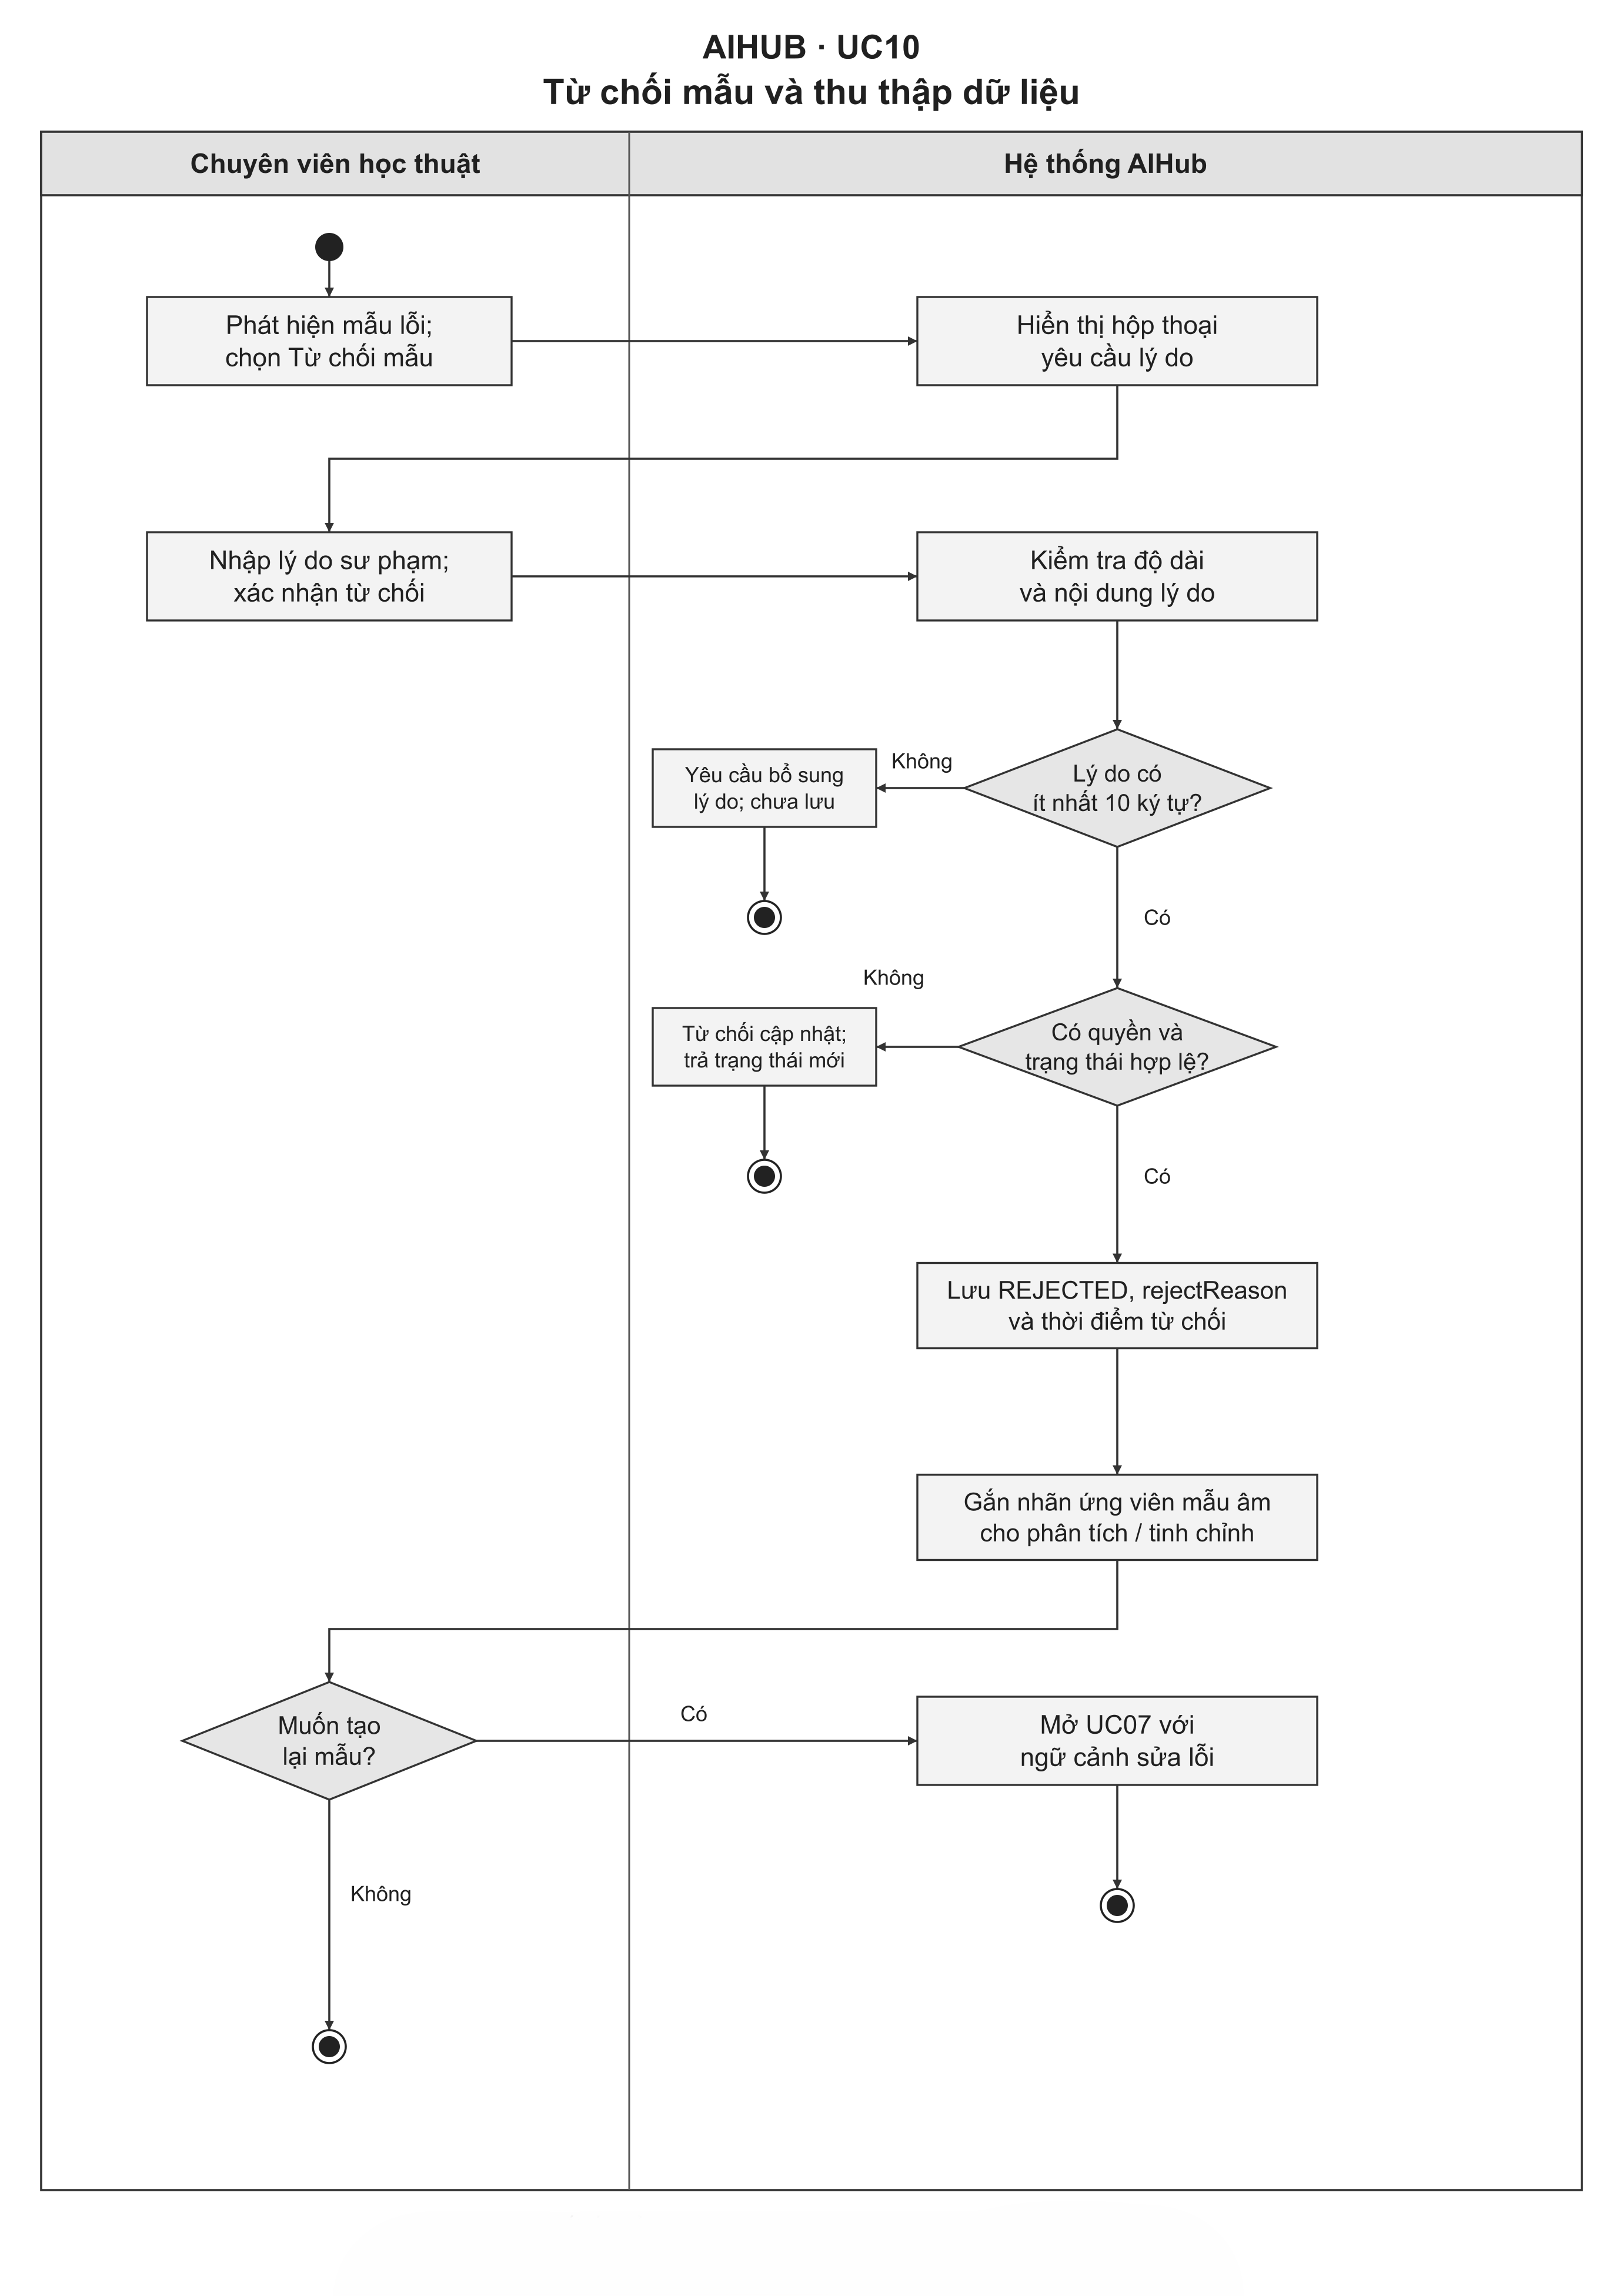
\includegraphics[width=\linewidth,height=0.72\textheight,keepaspectratio]{Images/Activity/AIHub/activity_uc10_reject_sample.png}
    \caption{Sơ đồ hoạt động AIHub -- Use-case 10: Từ chối mẫu và thu thập dữ liệu}
    \label{aihub:fig:activity_uc10}
    \label{aihub:fig:act_uc10_academic_reject}
\end{figure}

Chuyên viên chọn từ chối mẫu và nhập lý do. Dữ liệu được ghi nhận để phân tích lỗi và chuẩn bị dữ liệu tinh chỉnh.
% activity-generated:end


\clearpage

\paragraph{Luồng hoạt động: Quản lý kho dữ liệu mẫu học thuật (Use-case 11)}

% activity-generated:start
\begin{figure}[H]
    \centering
    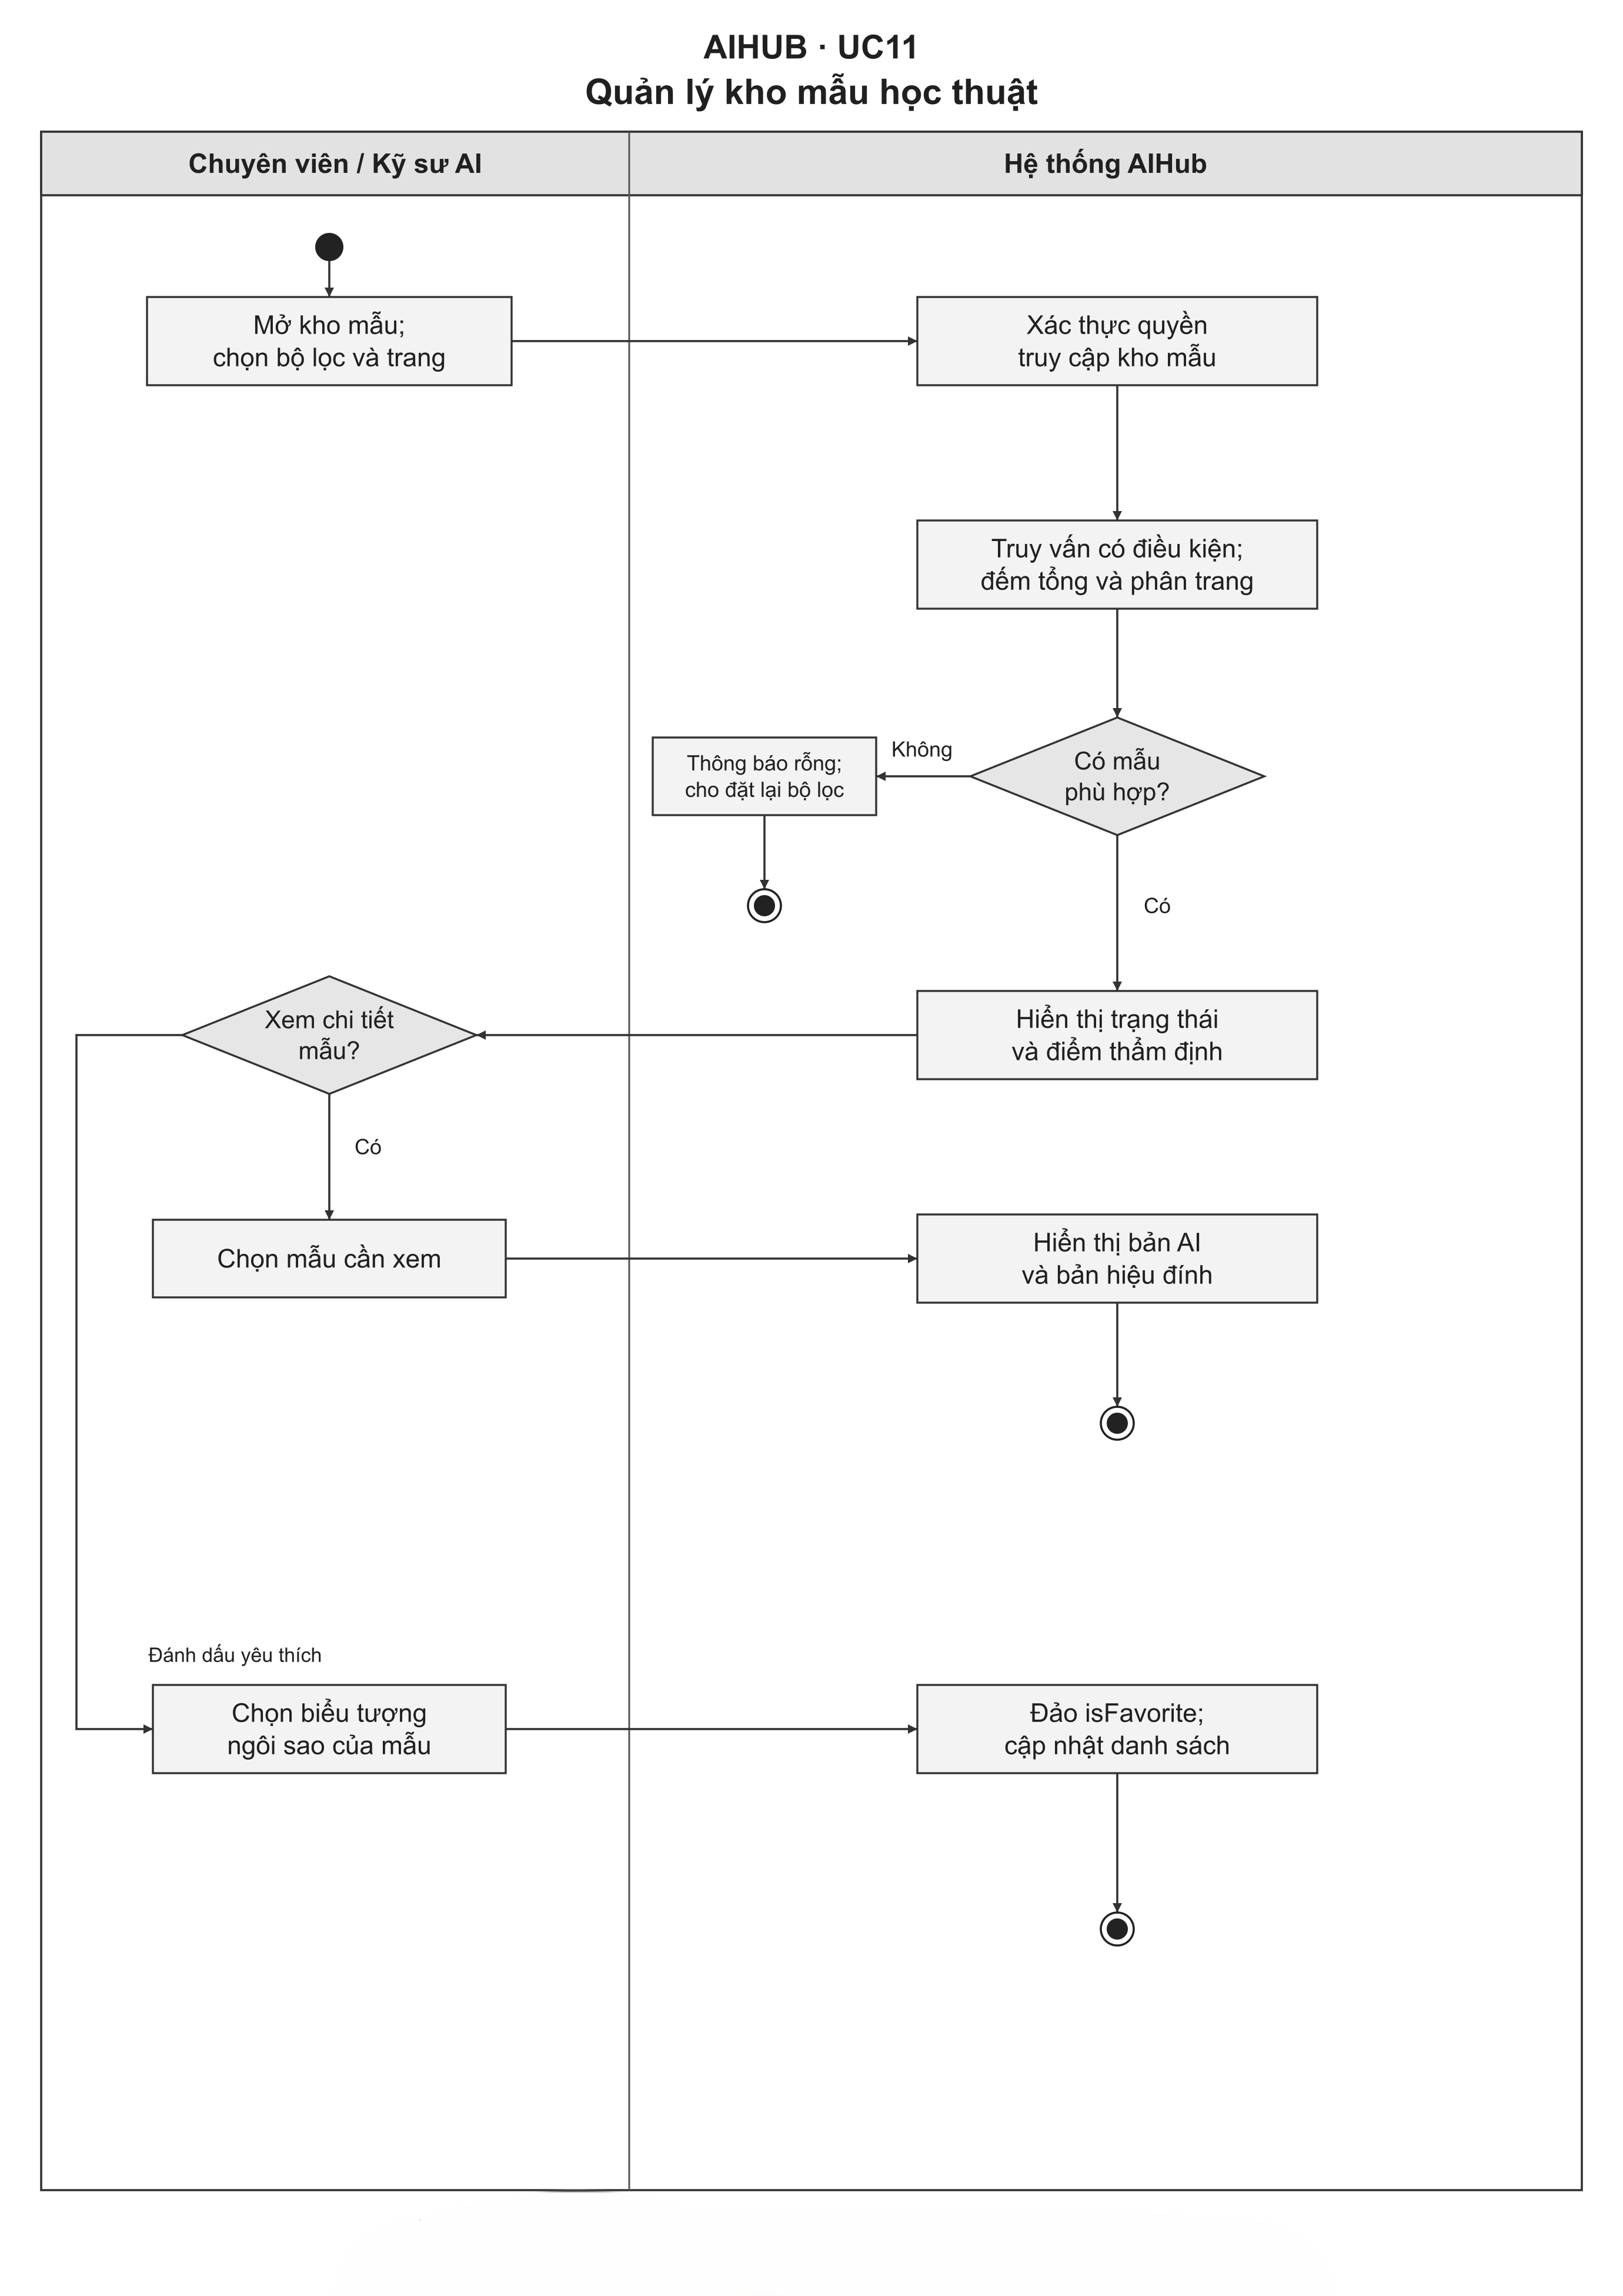
\includegraphics[width=\linewidth,height=0.72\textheight,keepaspectratio]{Images/Activity/AIHub/activity_uc11_academic_inventory.png}
    \caption{Sơ đồ hoạt động AIHub -- Use-case 11: Quản lý kho mẫu học thuật}
    \label{aihub:fig:activity_uc11}
    \label{aihub:fig:act_uc11_academic_inventory}
\end{figure}

Chuyên viên chọn bộ lọc để tra cứu kho mẫu. Thao tác đánh dấu yêu thích được lưu mà không thay đổi trạng thái thẩm định.
% activity-generated:end


% =========================================================================
% NHÓM 3: KỸ SƯ AI (USE-CASE 12 - 15)
% =========================================================================

\clearpage

\paragraph{Luồng hoạt động: Cấu hình mẫu Prompt (Use-case 12)}

% activity-generated:start
\begin{figure}[H]
    \centering
    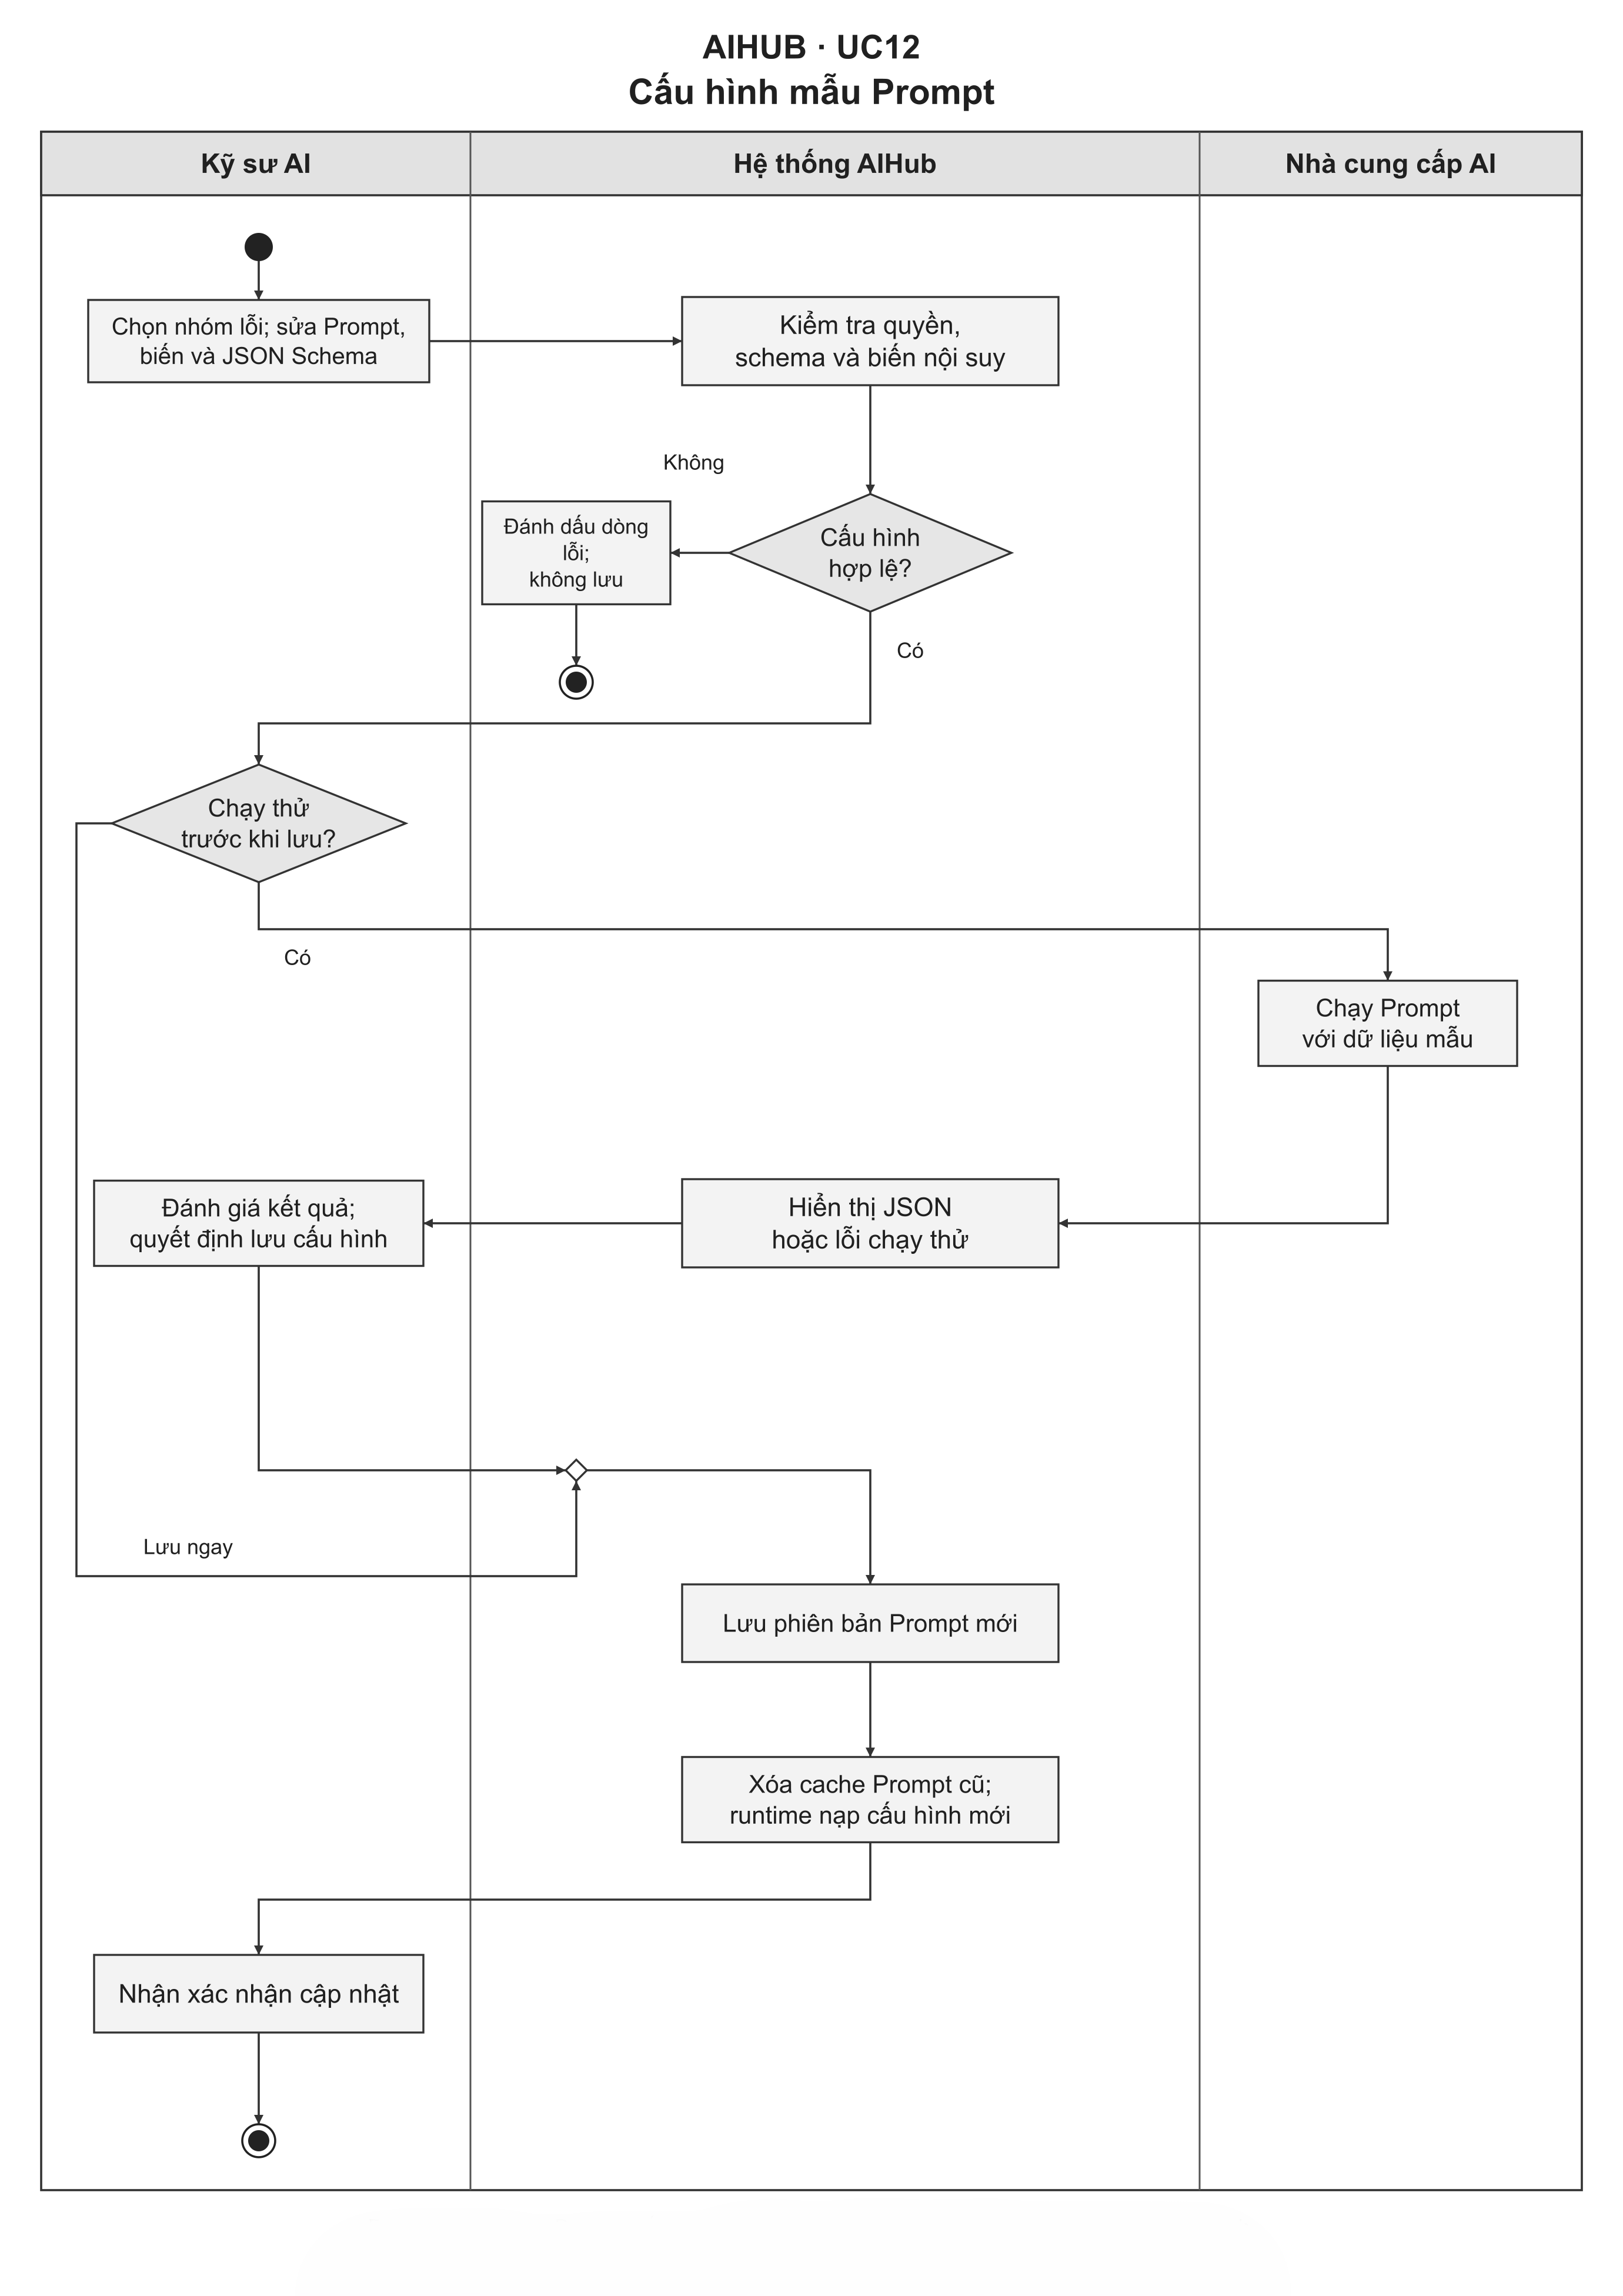
\includegraphics[width=\linewidth,height=0.72\textheight,keepaspectratio]{Images/Activity/AIHub/activity_uc12_prompt_templates.png}
    \caption{Sơ đồ hoạt động AIHub -- Use-case 12: Cấu hình mẫu Prompt}
    \label{aihub:fig:activity_uc12}
    \label{aihub:fig:act_uc12_config_prompt}
\end{figure}

Quản trị viên mở cấu hình và chỉnh sửa mẫu Prompt. Hệ thống lưu phiên bản mới và cập nhật cấu hình được sử dụng.
% activity-generated:end


\clearpage

\paragraph{Luồng hoạt động: Cấu hình chuỗi mô hình dự phòng (Use-case 13)}

% activity-generated:start
\begin{figure}[H]
    \centering
    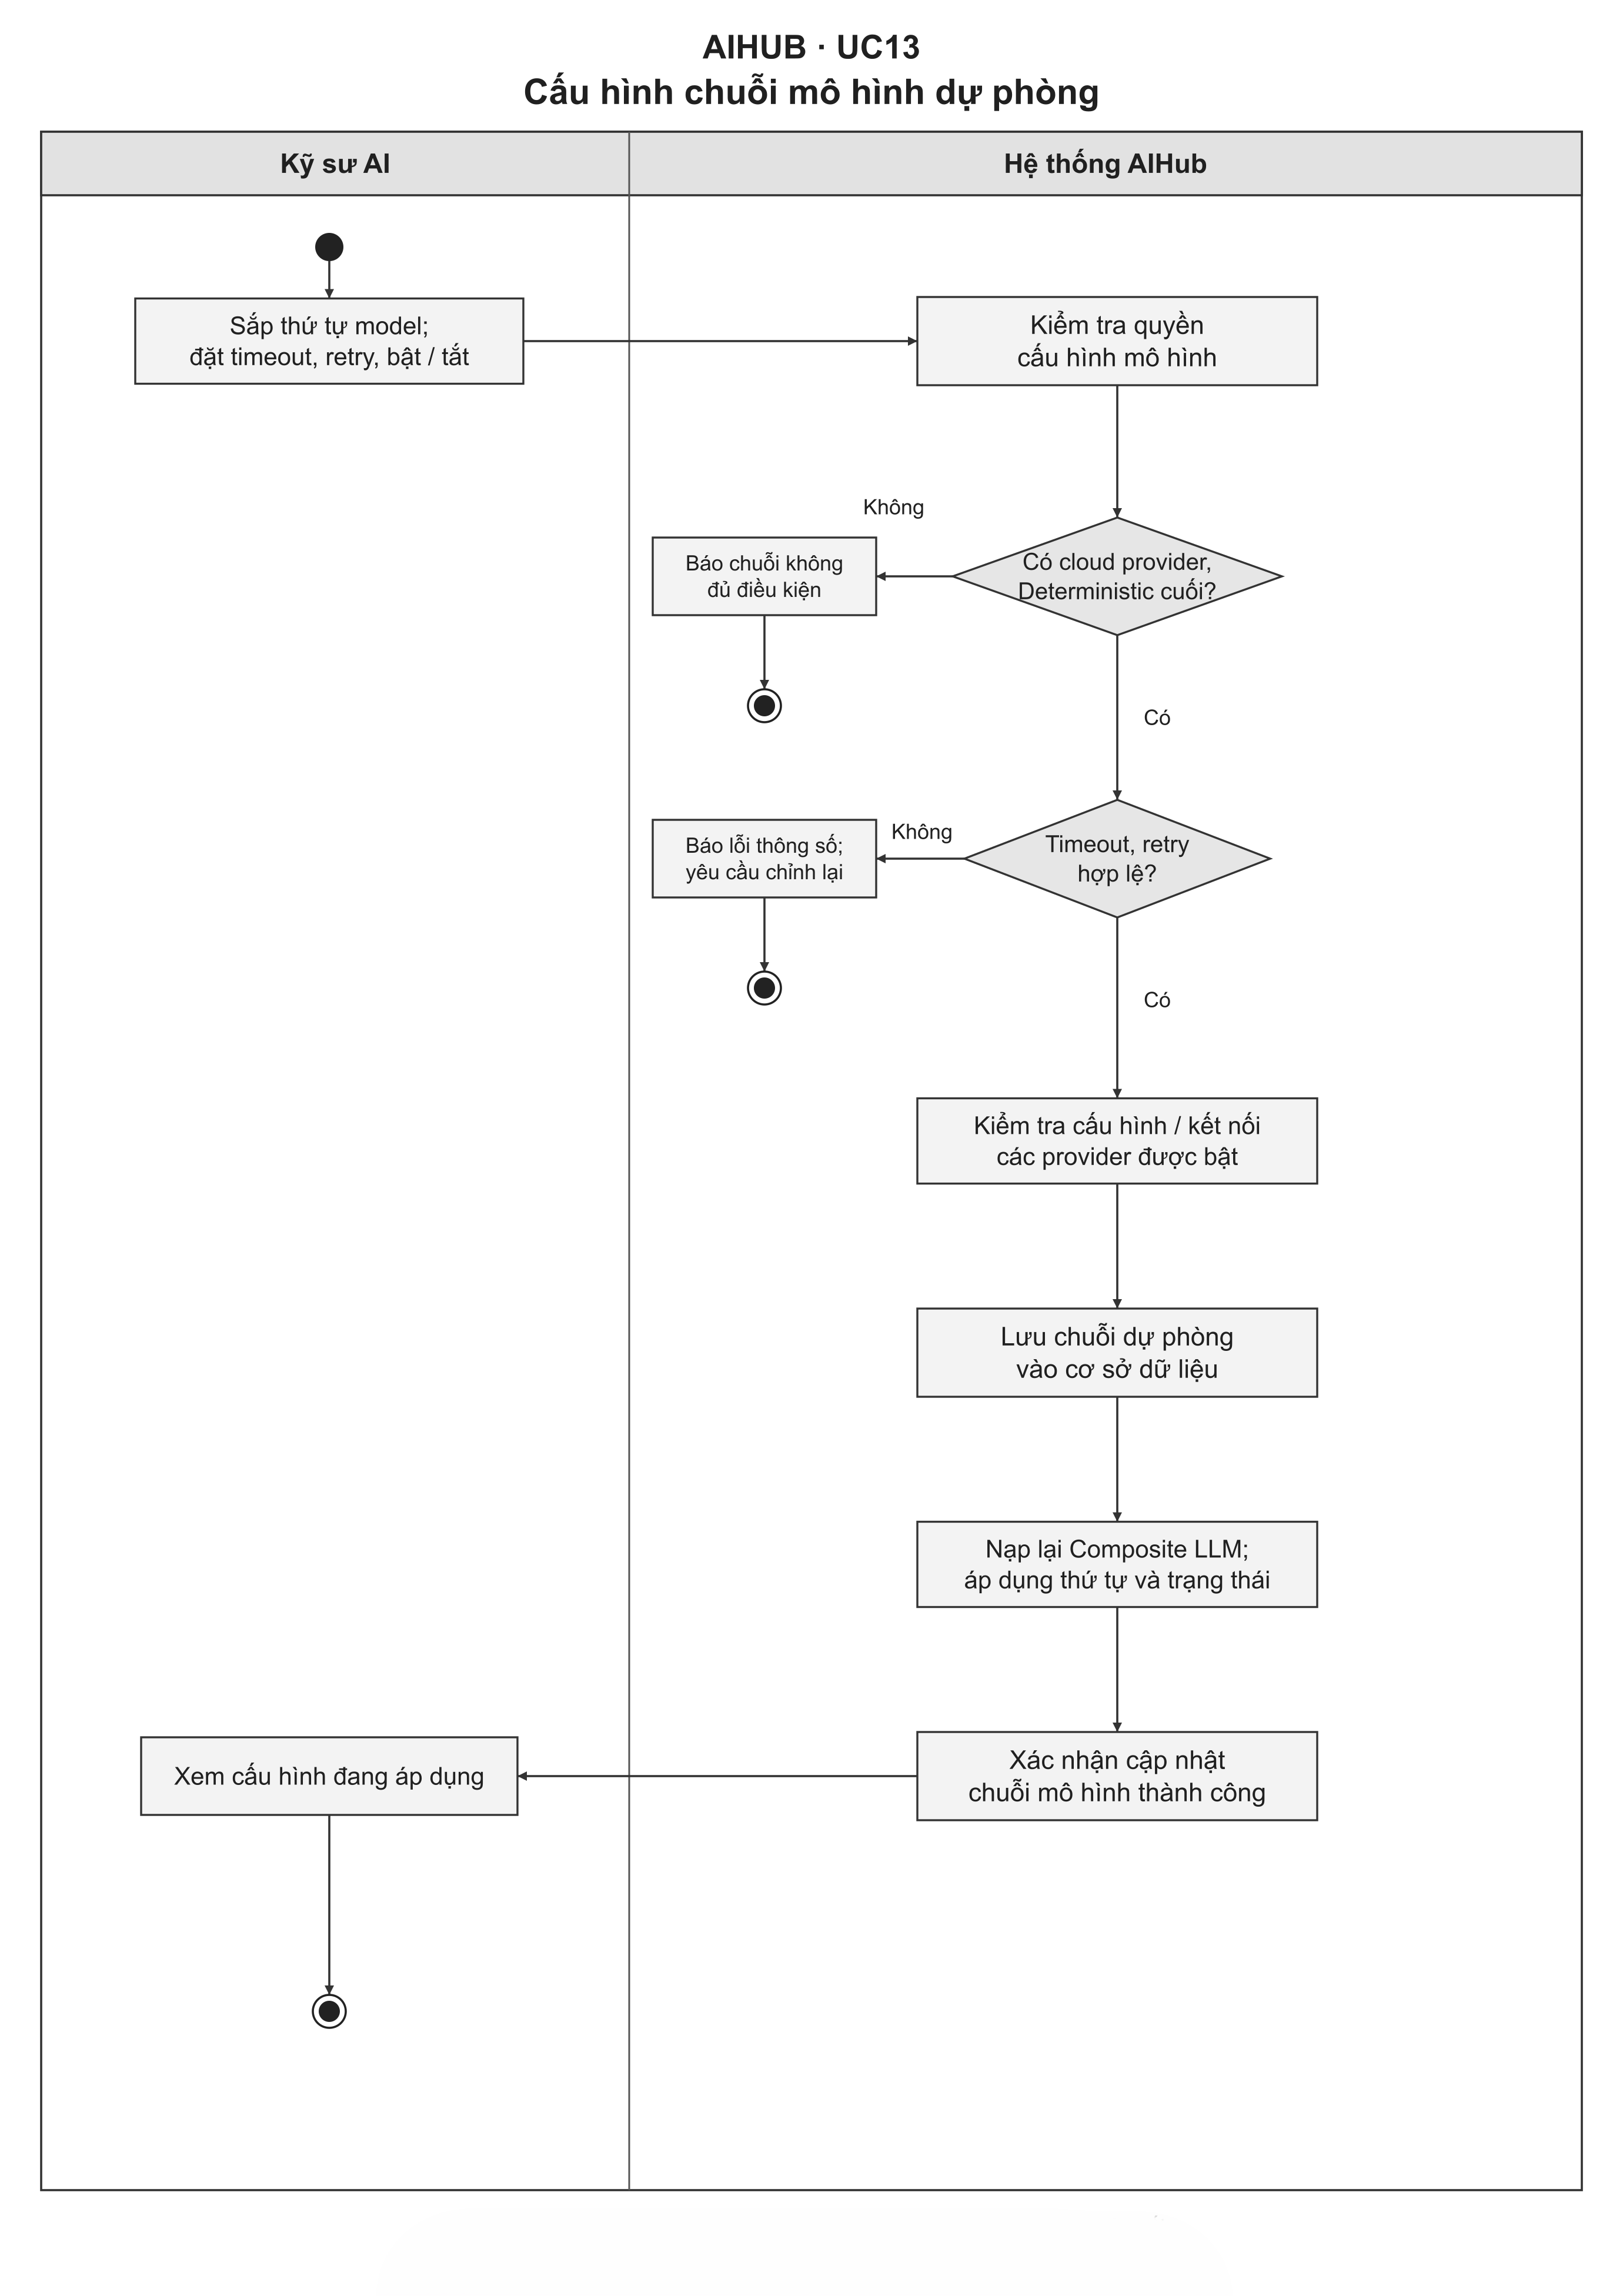
\includegraphics[width=\linewidth,height=0.72\textheight,keepaspectratio]{Images/Activity/AIHub/activity_uc13_model_fallback.png}
    \caption{Sơ đồ hoạt động AIHub -- Use-case 13: Cấu hình chuỗi mô hình dự phòng}
    \label{aihub:fig:activity_uc13}
    \label{aihub:fig:act_uc13_config_fallback}
\end{figure}

Quản trị viên chỉnh thứ tự, thời gian chờ và số lần thử của các mô hình. Hệ thống cập nhật chuỗi gọi mô hình và thông báo kết quả.
% activity-generated:end


\clearpage

\paragraph{Luồng hoạt động: Trích xuất tập dữ liệu tinh chỉnh SFT/DPO (Use-case 14)}

% activity-generated:start
\begin{figure}[H]
    \centering
    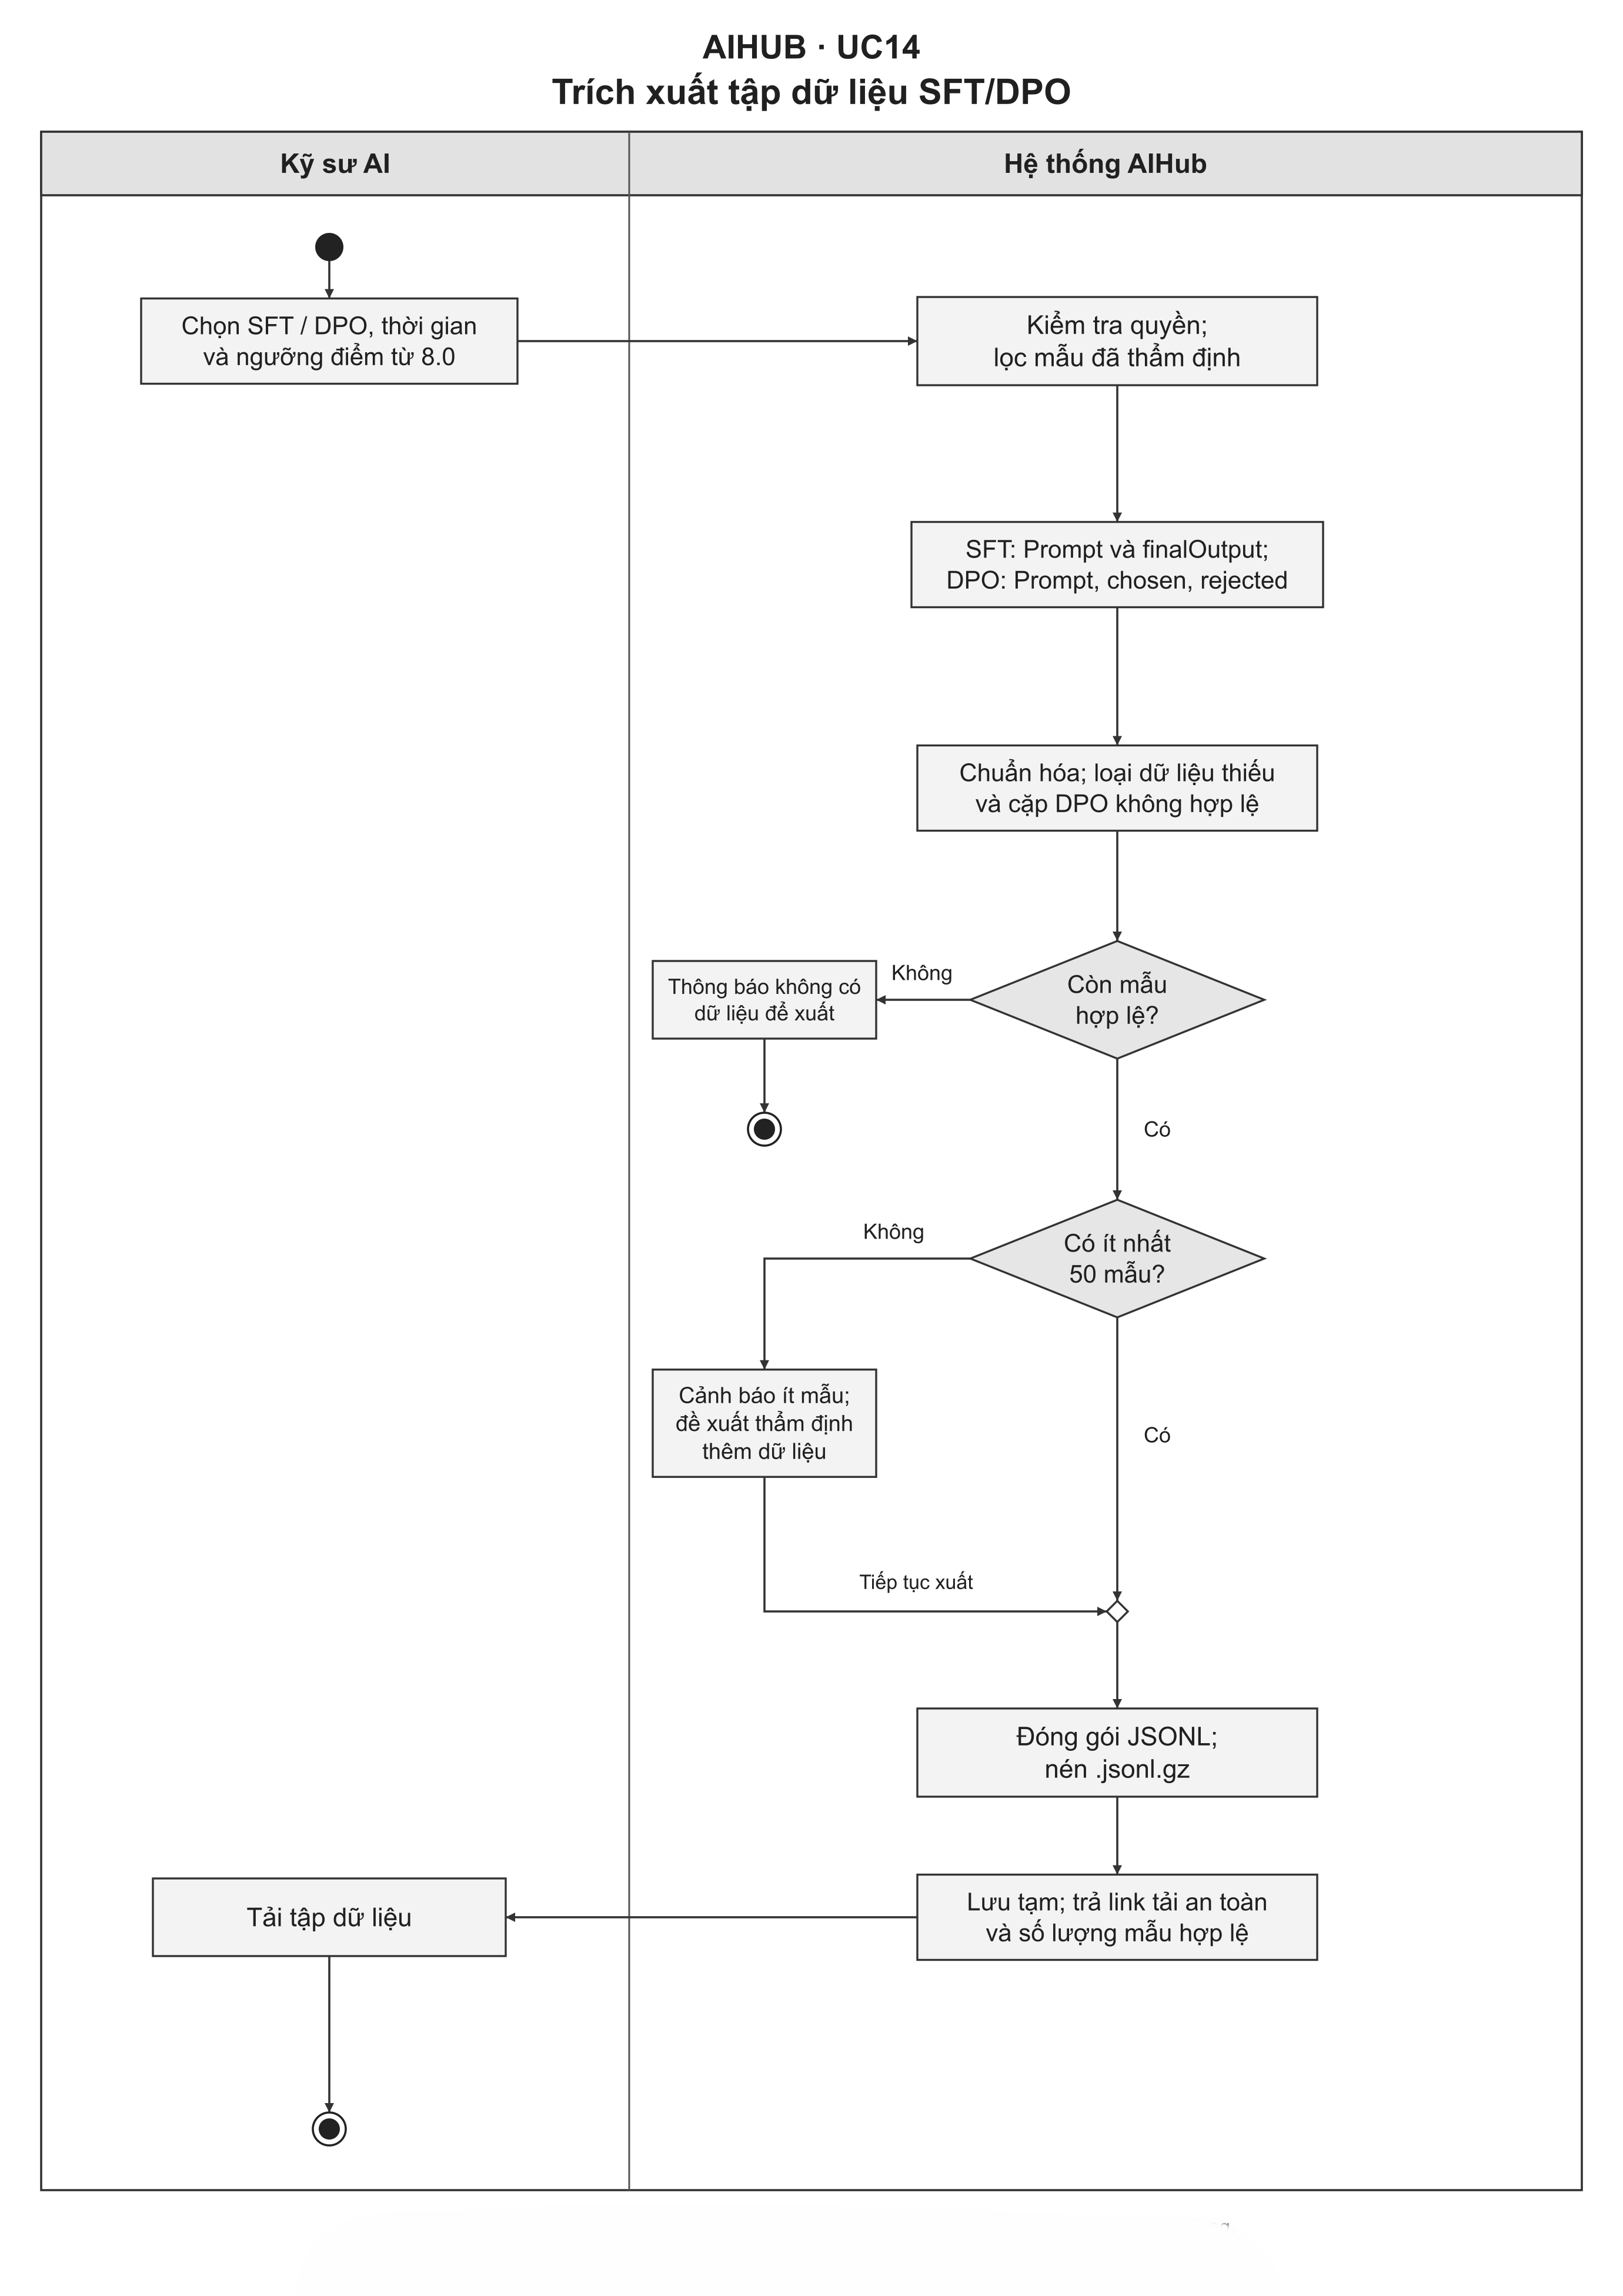
\includegraphics[width=\linewidth,height=0.72\textheight,keepaspectratio]{Images/Activity/AIHub/activity_uc14_export_datasets.png}
    \caption{Sơ đồ hoạt động AIHub -- Use-case 14: Trích xuất tập dữ liệu SFT/DPO}
    \label{aihub:fig:activity_uc14}
    \label{aihub:fig:act_uc14_export_datasets}
\end{figure}

Chuyên viên chọn loại dữ liệu SFT hoặc DPO và phạm vi xuất. Tập dữ liệu được tạo và cung cấp để tải xuống.
% activity-generated:end


\clearpage

\paragraph{Luồng hoạt động: Theo dõi và phân tích lỗi mô hình (Use-case 15)}

% activity-generated:start
\begin{figure}[H]
    \centering
    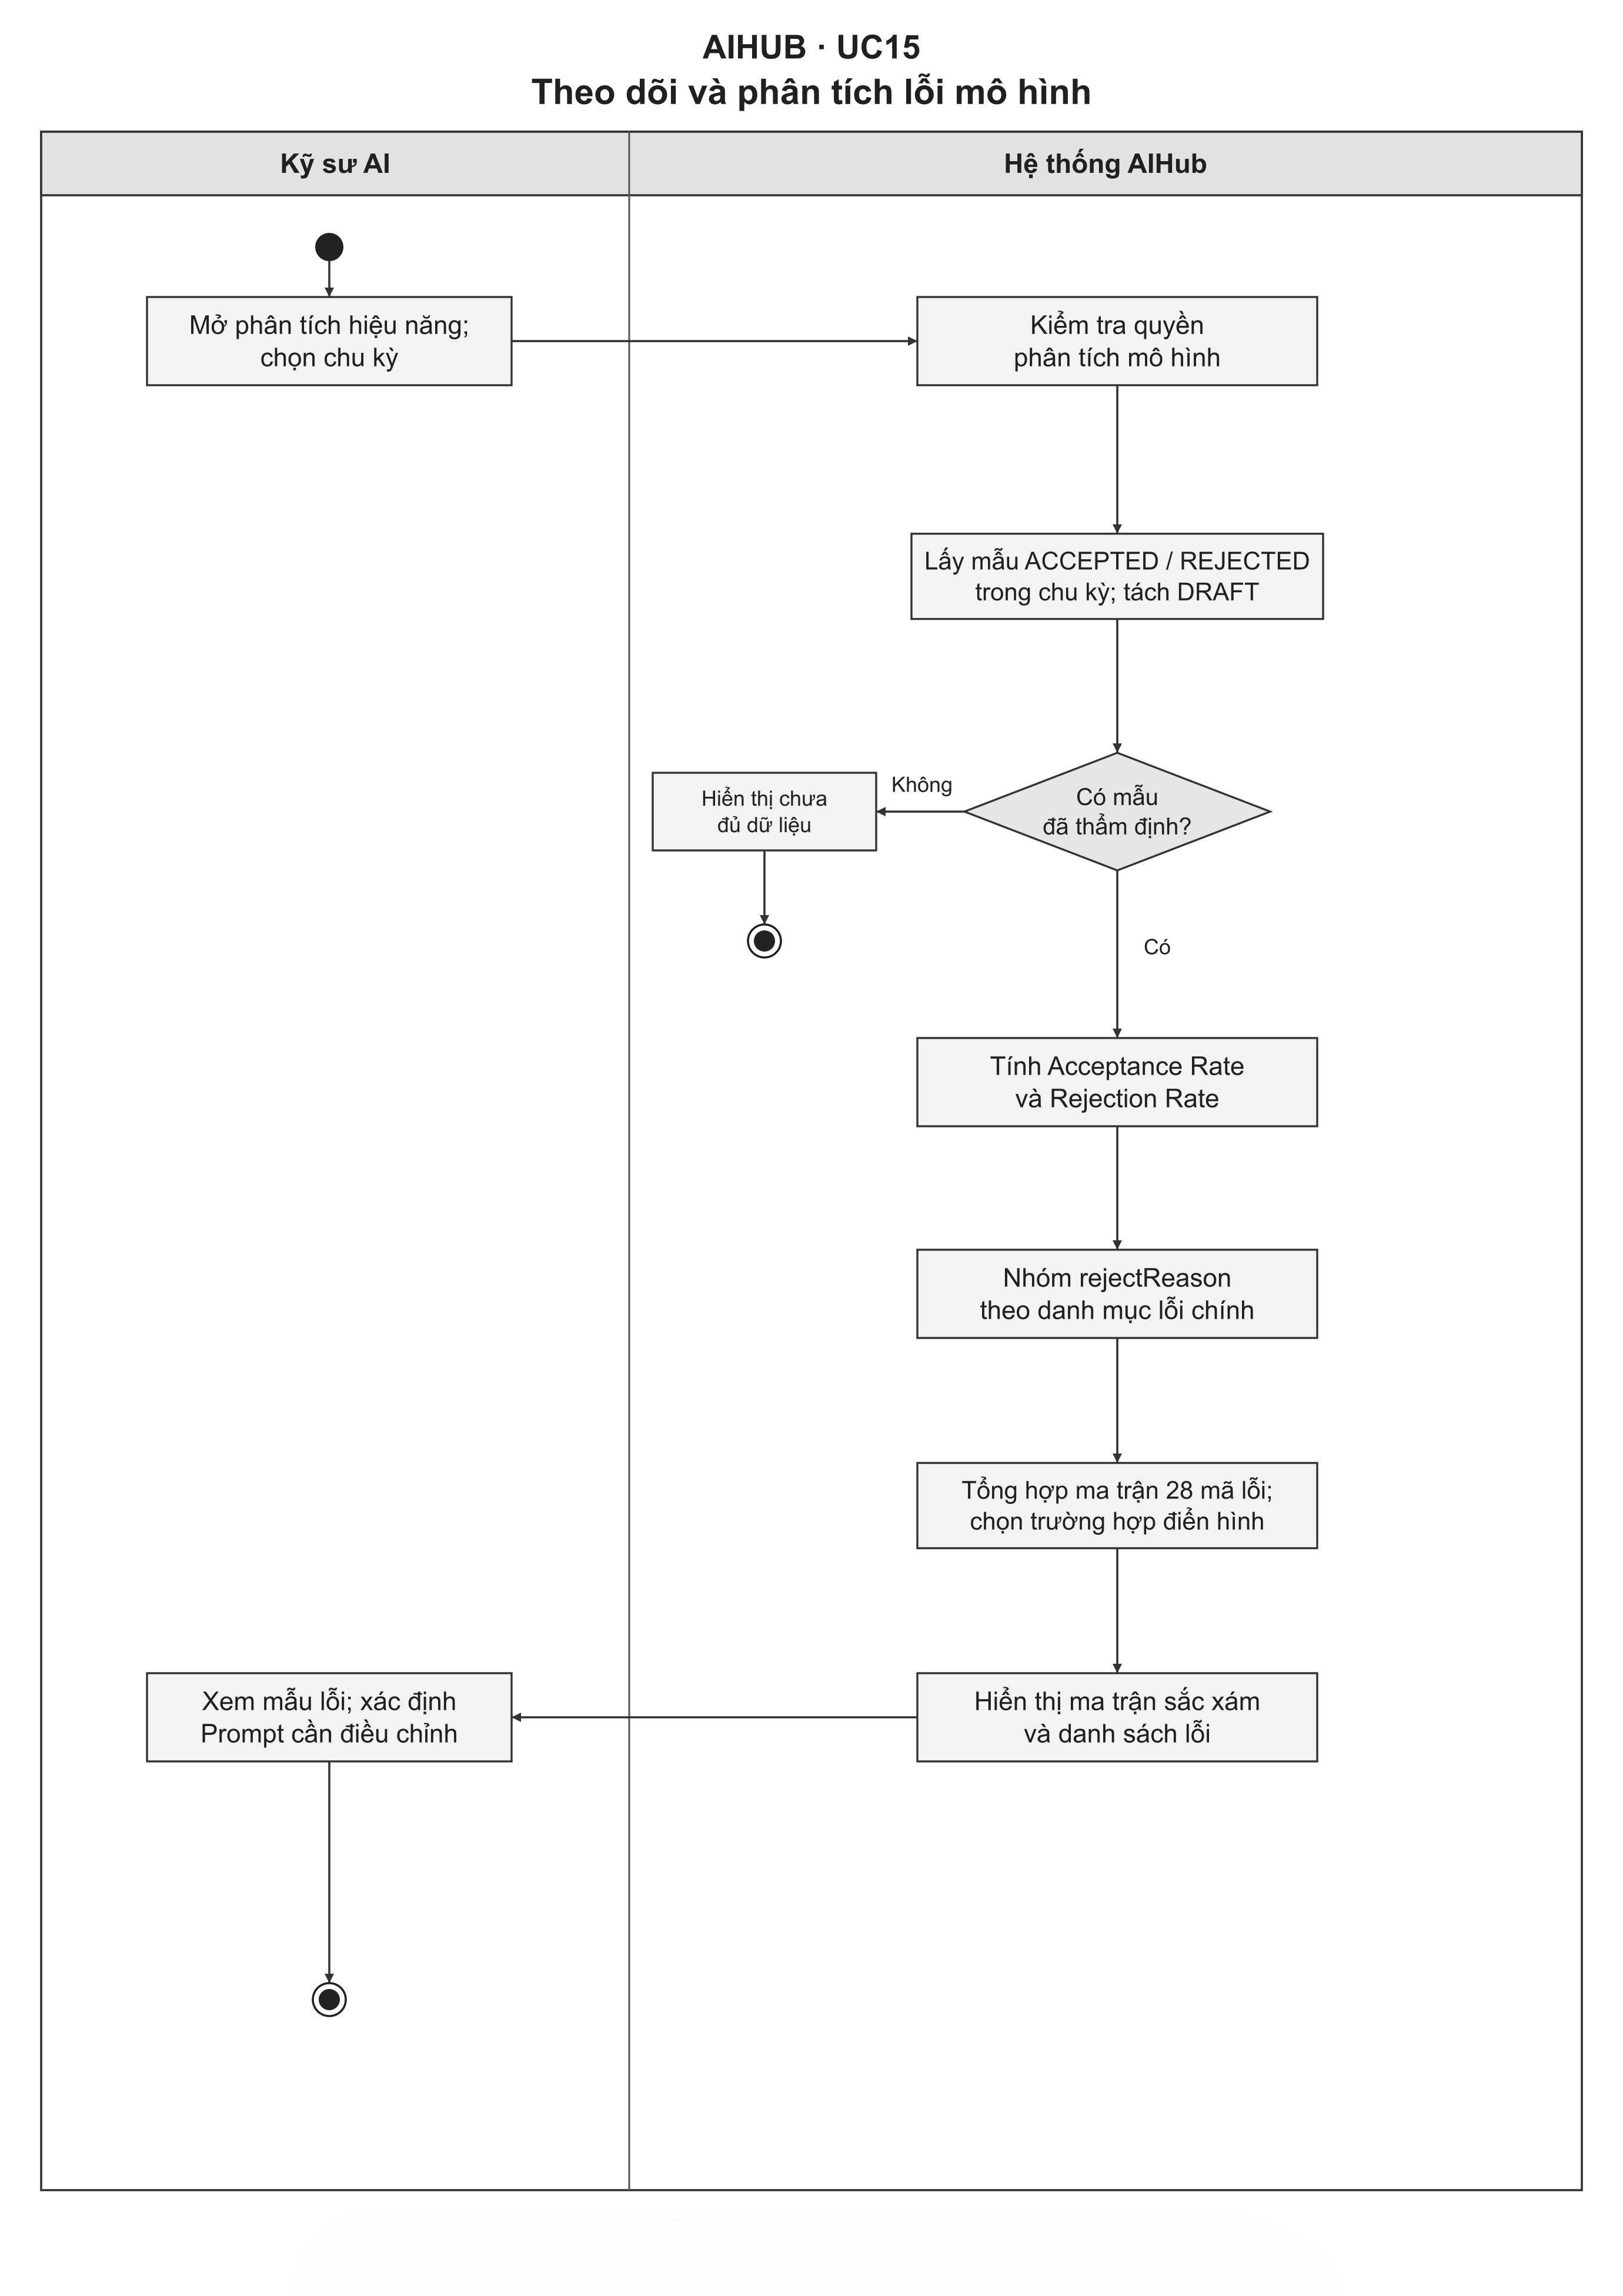
\includegraphics[width=\linewidth,height=0.72\textheight,keepaspectratio]{Images/Activity/AIHub/activity_uc15_model_error_analysis.png}
    \caption{Sơ đồ hoạt động AIHub -- Use-case 15: Theo dõi và phân tích lỗi mô hình}
    \label{aihub:fig:activity_uc15}
    \label{aihub:fig:act_uc15_analyze_model_errors}
\end{figure}

Người dùng chọn bộ lọc thống kê chất lượng mô hình. Người dùng xem chi tiết nhóm lỗi để xác định nội dung cần cải thiện.
% activity-generated:end


% =========================================================================
% NHÓM 4: QUẢN TRỊ VIÊN TỔ CHỨC & NỀN TẢNG (USE-CASE 16 - 20)
% =========================================================================

\clearpage

\paragraph{Luồng hoạt động: Quản lý thành viên tổ chức (Use-case 16)}

% activity-generated:start
\begin{figure}[H]
    \centering
    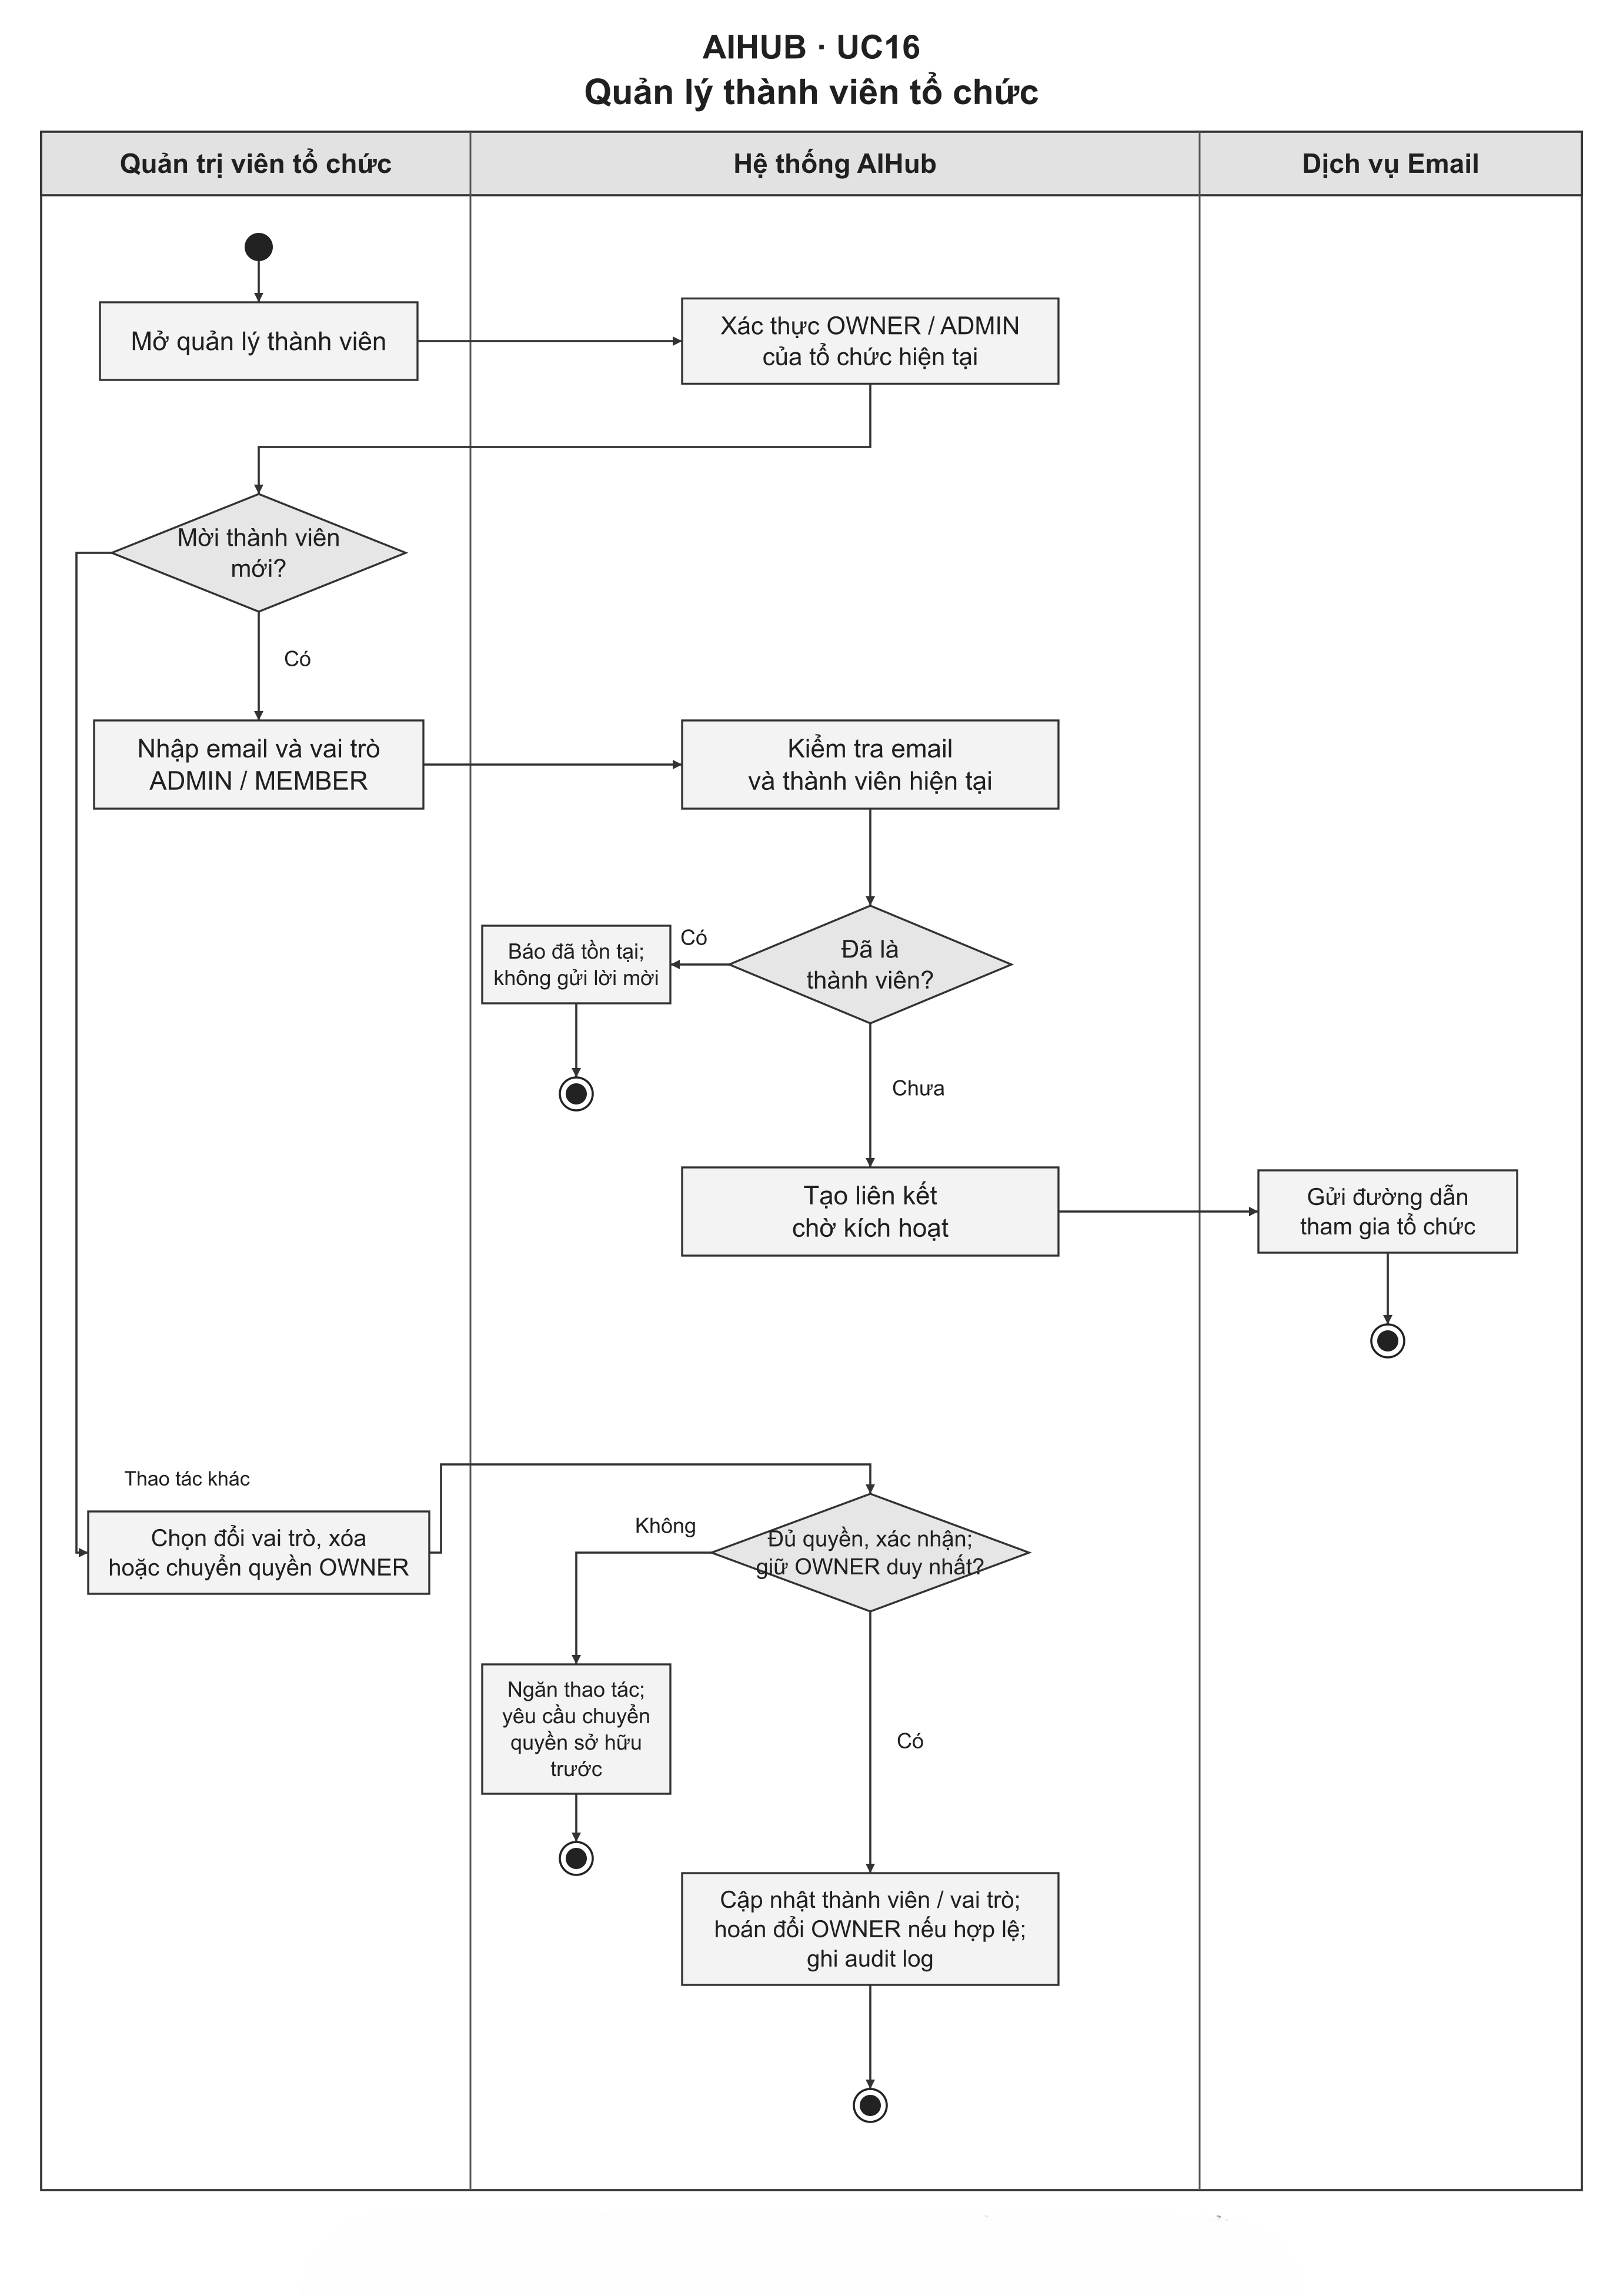
\includegraphics[width=\linewidth,height=0.72\textheight,keepaspectratio]{Images/Activity/AIHub/activity_uc16_organization_members.png}
    \caption{Sơ đồ hoạt động AIHub -- Use-case 16: Quản lý thành viên tổ chức}
    \label{aihub:fig:activity_uc16}
    \label{aihub:fig:act_uc16_manage_org_members}
\end{figure}

Người quản trị tổ chức chọn mời, đổi vai trò, xóa thành viên hoặc chuyển quyền. Hệ thống gửi thông báo và ghi nhật ký thay đổi.
% activity-generated:end


\clearpage

\paragraph{Luồng hoạt động: Quản trị gói cước và Hạn mức (Use-case 17)}

% activity-generated:start
\begin{figure}[H]
    \centering
    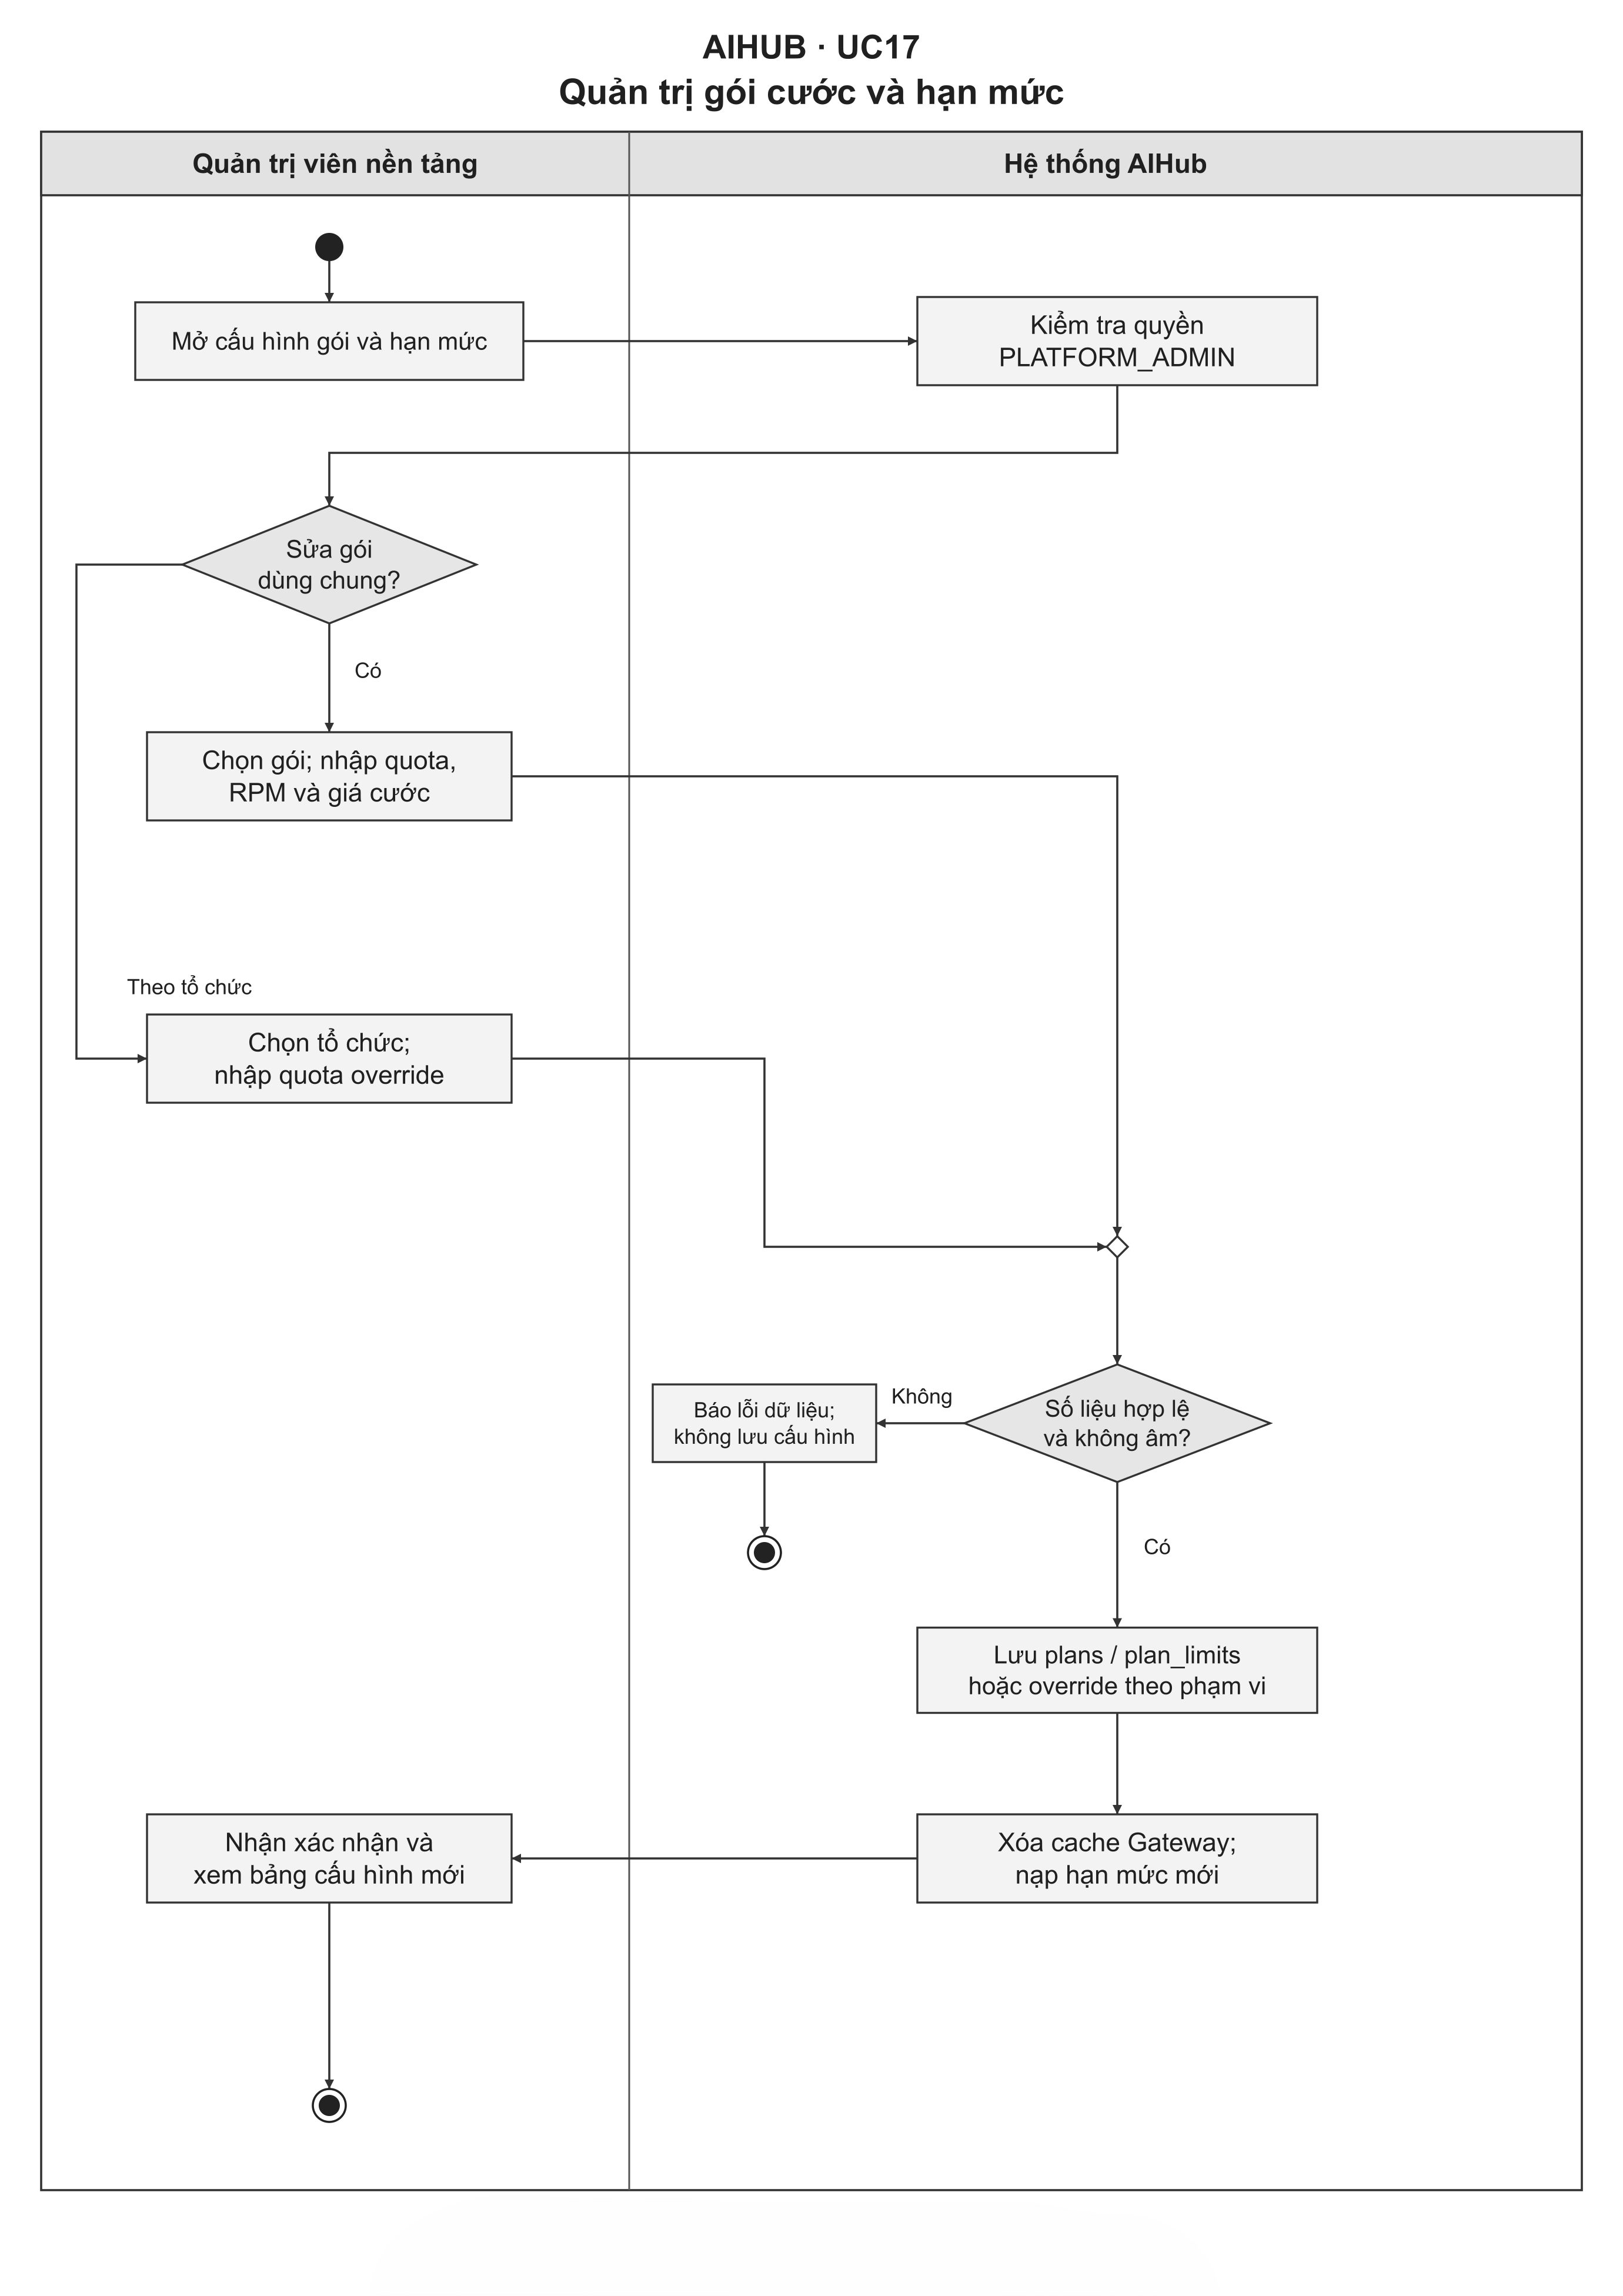
\includegraphics[width=\linewidth,height=0.72\textheight,keepaspectratio]{Images/Activity/AIHub/activity_uc17_plans_quota.png}
    \caption{Sơ đồ hoạt động AIHub -- Use-case 17: Quản trị gói cước và hạn mức}
    \label{aihub:fig:activity_uc17}
    \label{aihub:fig:act_uc17_config_plans}
\end{figure}

Quản trị viên chọn chỉnh gói dùng chung hoặc hạn mức riêng của tổ chức. Gateway cập nhật hạn mức và giao diện hiển thị kết quả.
% activity-generated:end


\clearpage

\paragraph{Luồng hoạt động: Giám sát trạng thái toàn hệ thống (Use-case 18)}

% activity-generated:start
\begin{figure}[H]
    \centering
    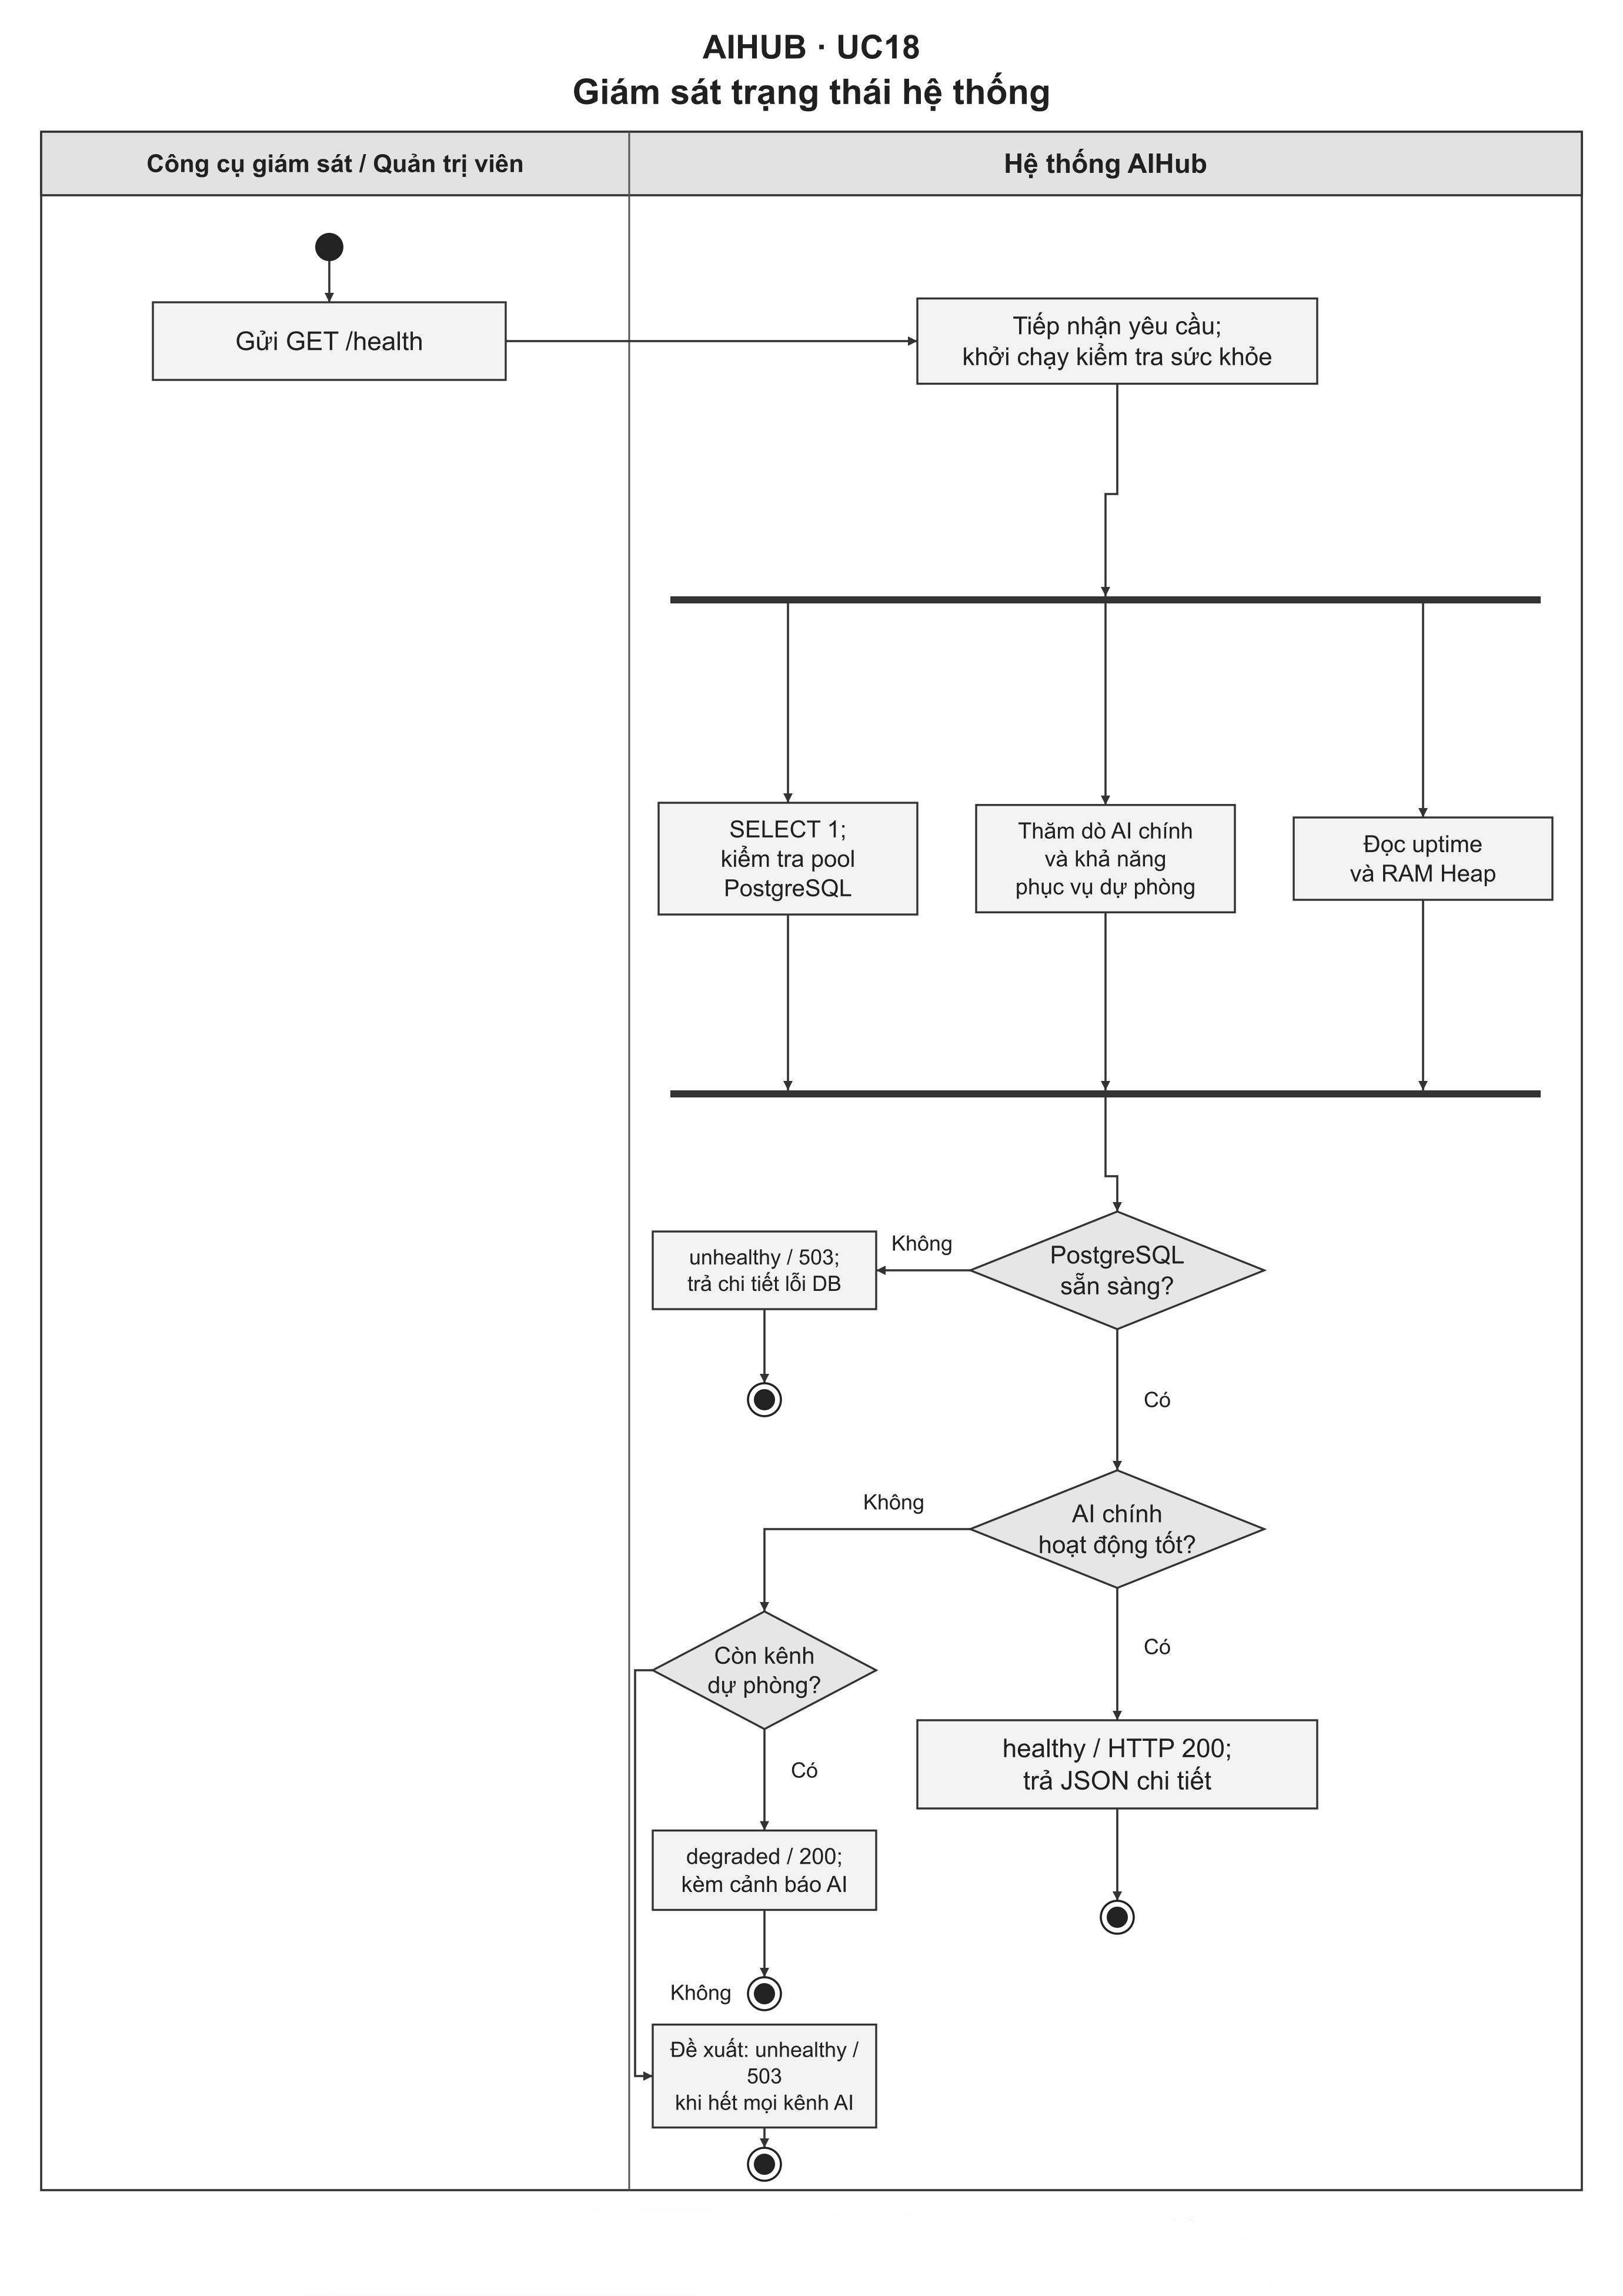
\includegraphics[width=\linewidth,height=0.72\textheight,keepaspectratio]{Images/Activity/AIHub/activity_uc18_system_health.png}
    \caption{Sơ đồ hoạt động AIHub -- Use-case 18: Giám sát trạng thái hệ thống}
    \label{aihub:fig:activity_uc18}
    \label{aihub:fig:act_uc18_health_probe}
\end{figure}

Công cụ giám sát hoặc quản trị viên gửi yêu cầu kiểm tra trạng thái. Hệ thống trả trạng thái hoạt động cùng mã phản hồi tương ứng.
% activity-generated:end


\clearpage

\paragraph{Luồng hoạt động: Quản lý danh mục Universal Specs (Use-case 19)}

% activity-generated:start
\begin{figure}[H]
    \centering
    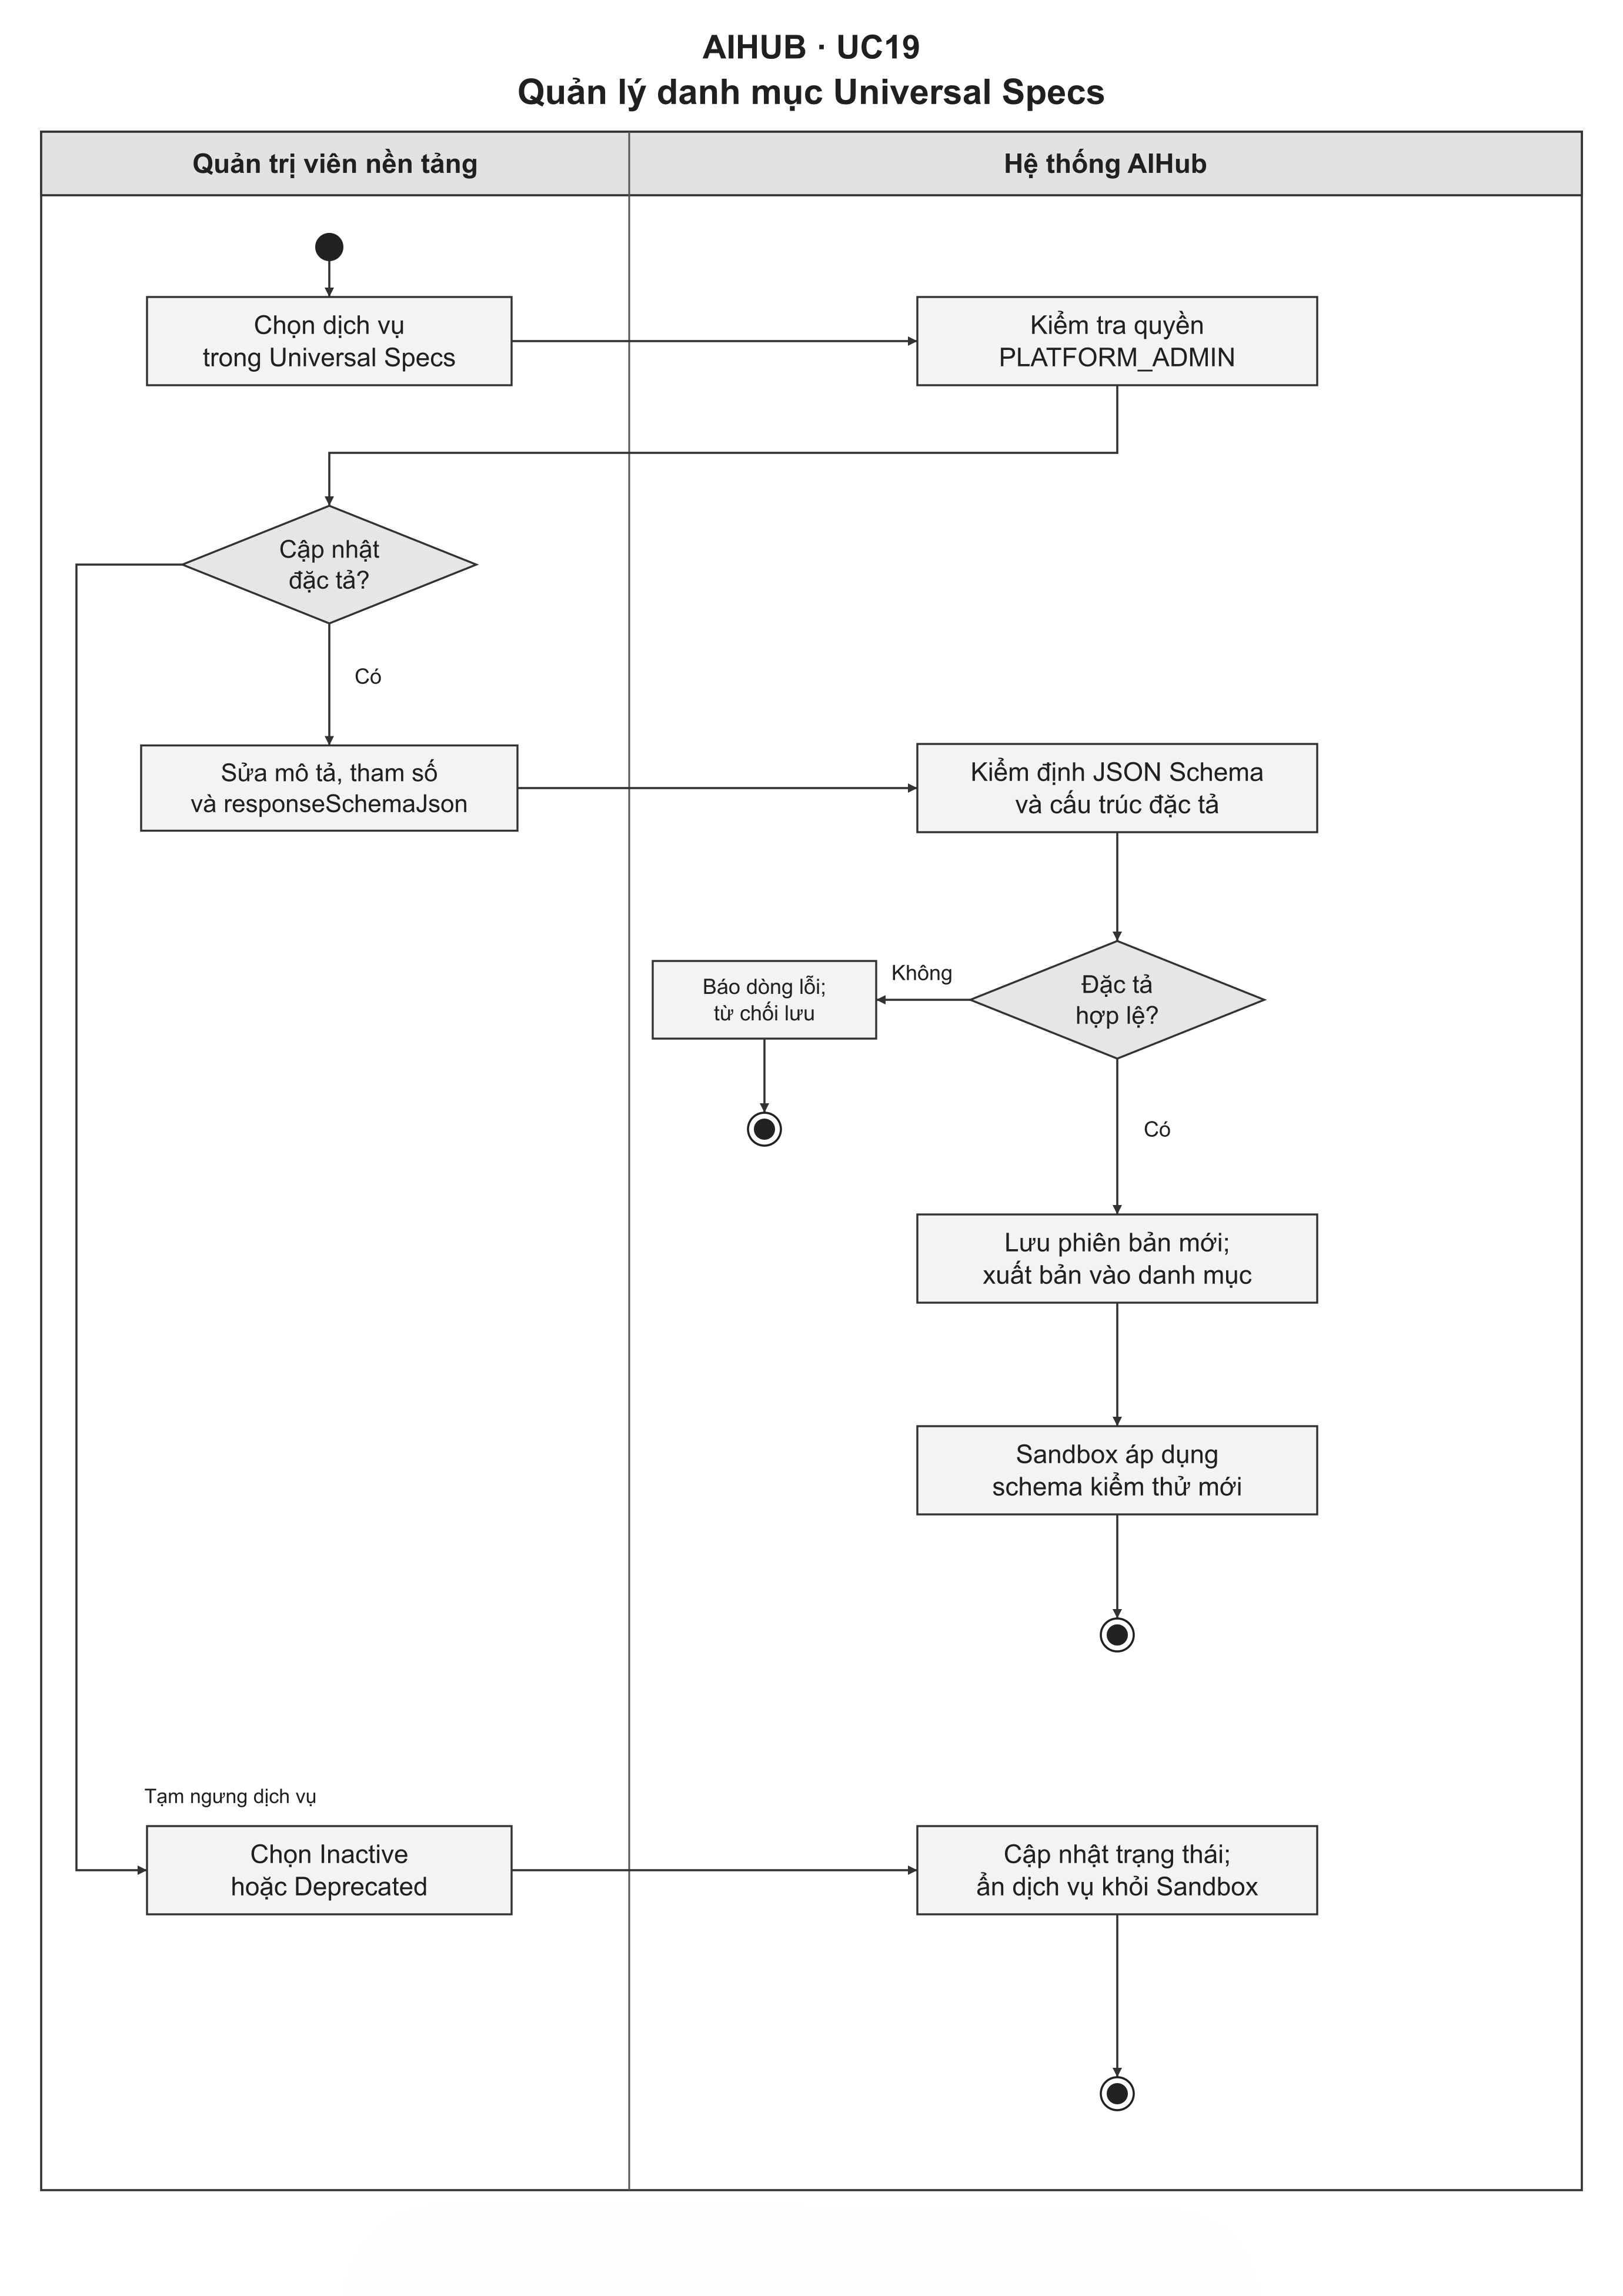
\includegraphics[width=\linewidth,height=0.72\textheight,keepaspectratio]{Images/Activity/AIHub/activity_uc19_universal_specs.png}
    \caption{Sơ đồ hoạt động AIHub -- Use-case 19: Quản lý danh mục Universal Specs}
    \label{aihub:fig:activity_uc19}
    \label{aihub:fig:act_uc19_manage_universal_specs}
\end{figure}

Quản trị viên tạo hoặc cập nhật đặc tả dịch vụ. Danh mục và khả năng chạy thử trong Sandbox được cập nhật tương ứng.
% activity-generated:end


\clearpage

\paragraph{Luồng hoạt động: Kiểm toán hệ thống và truy vết giao dịch (Use-case 20)}

% activity-generated:start
\begin{figure}[H]
    \centering
    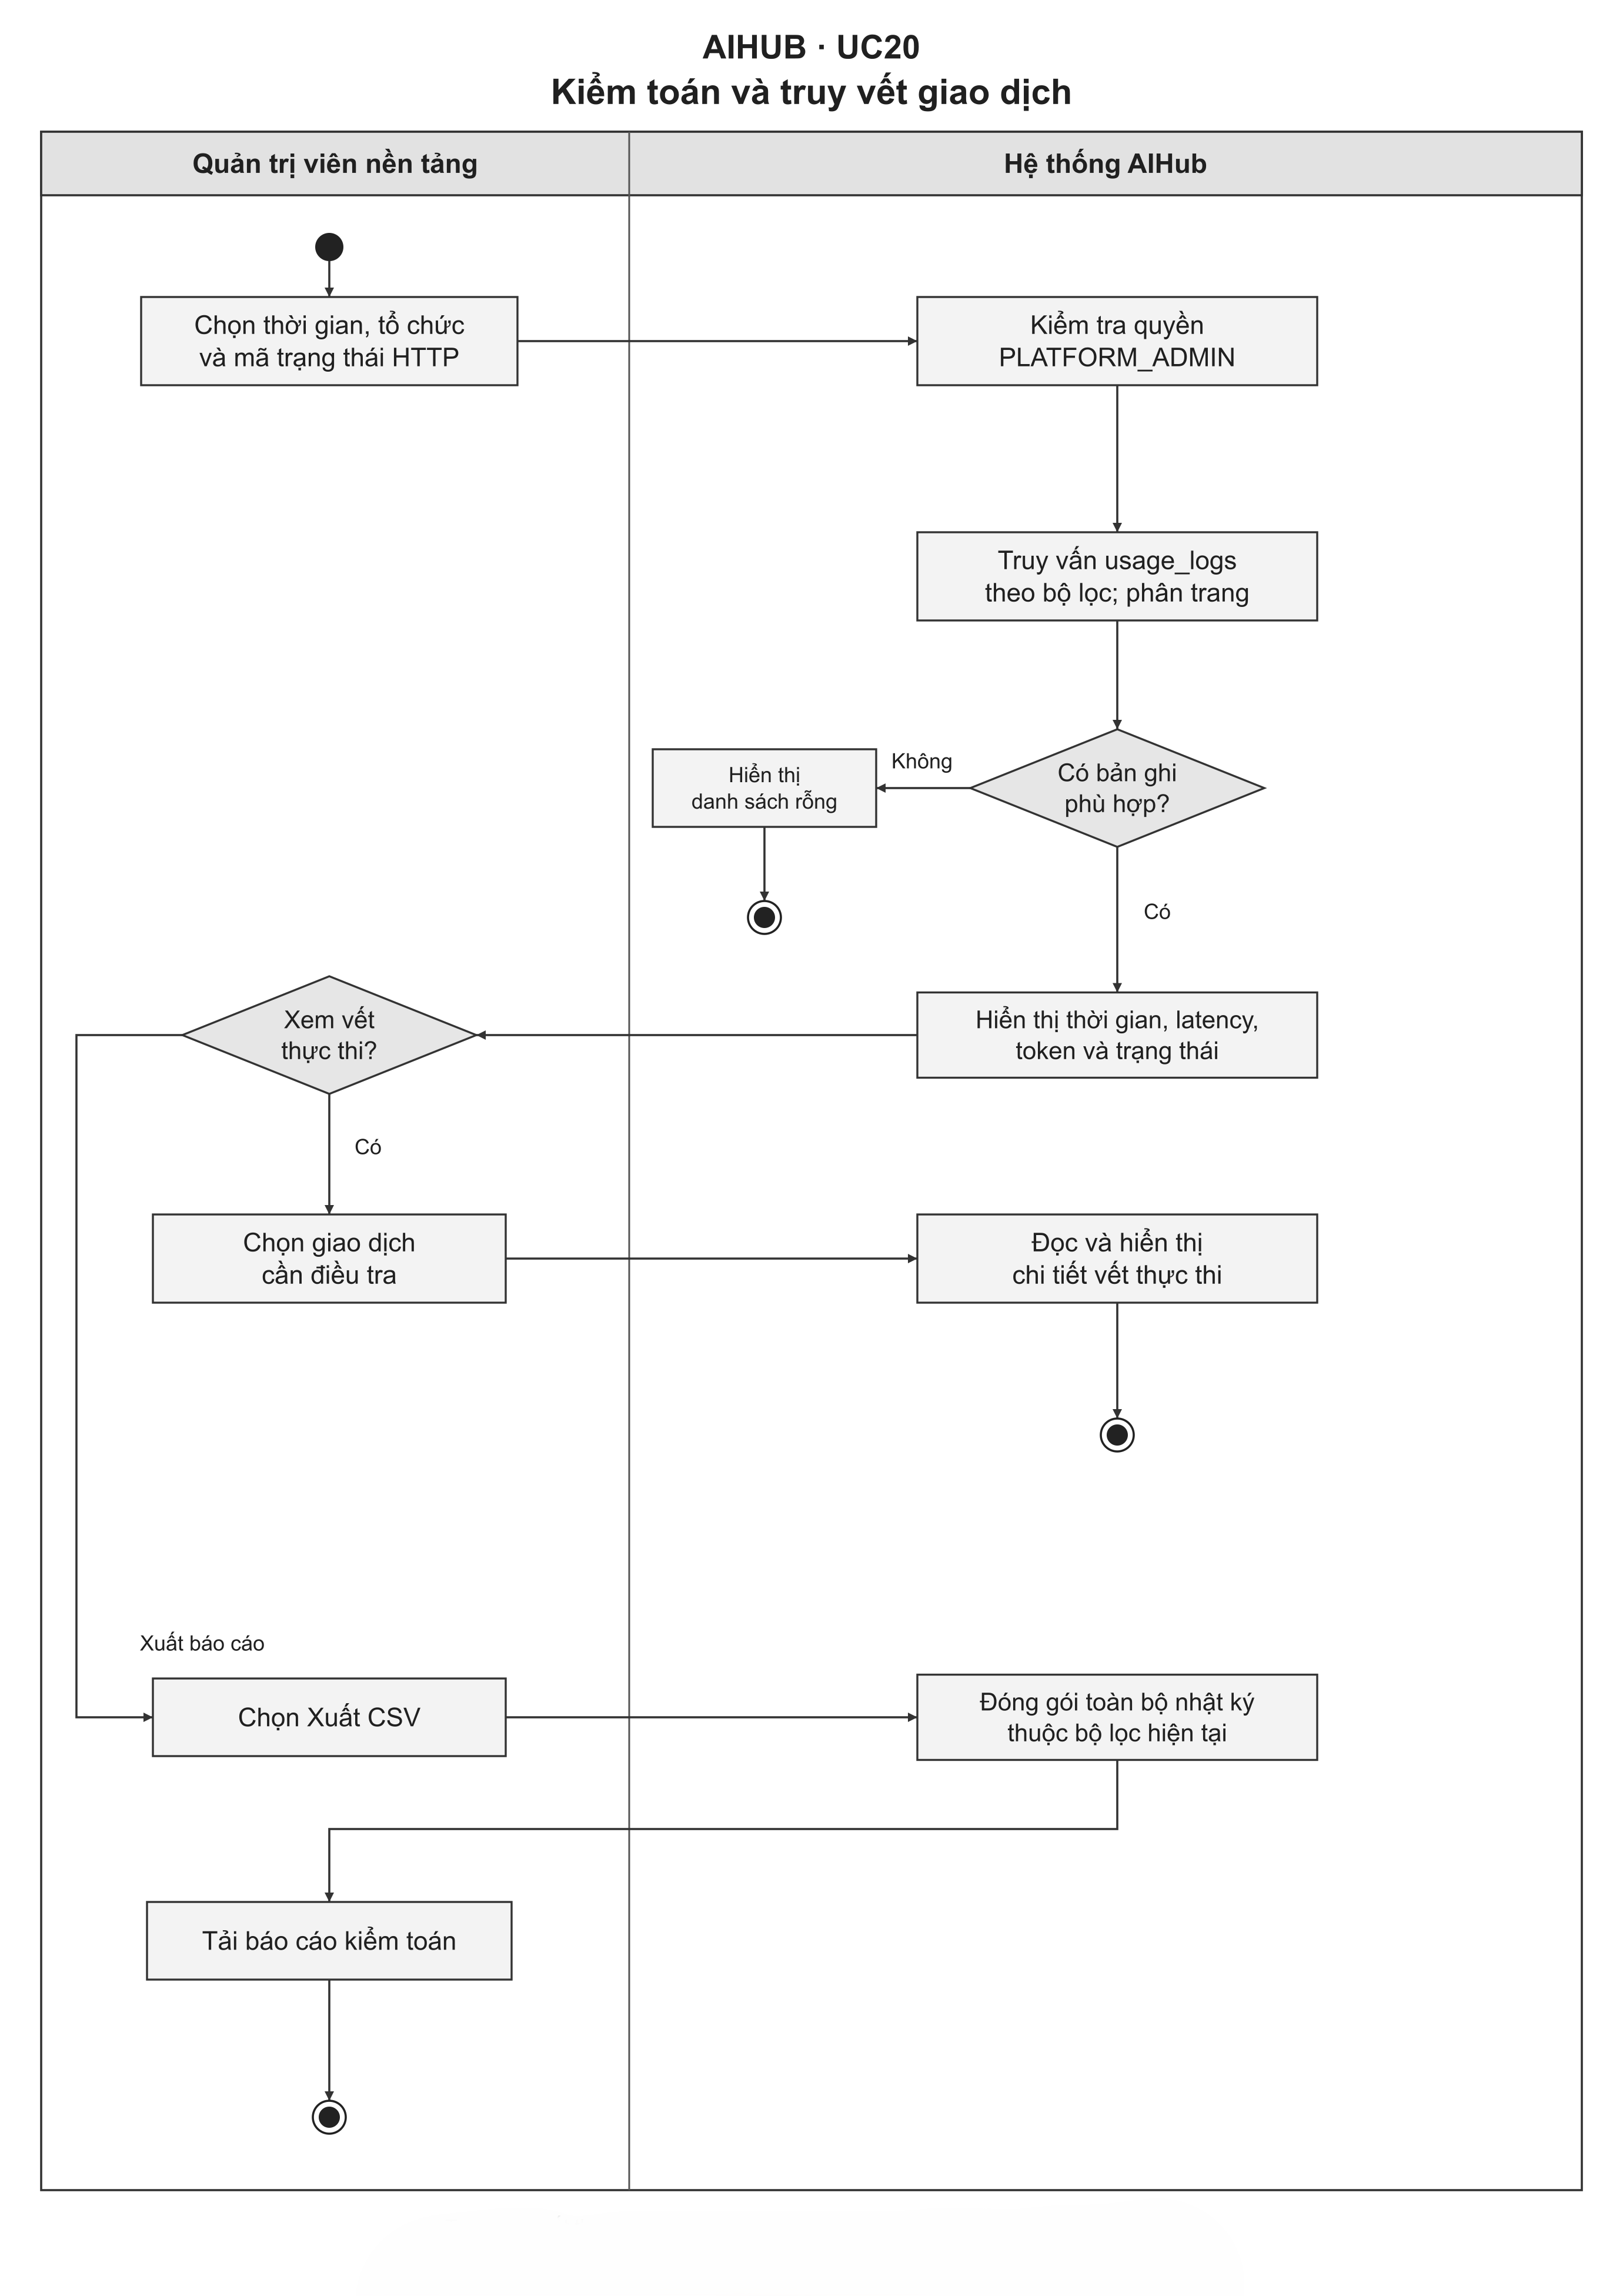
\includegraphics[width=\linewidth,height=0.72\textheight,keepaspectratio]{Images/Activity/AIHub/activity_uc20_audit_logs.png}
    \caption{Sơ đồ hoạt động AIHub -- Use-case 20: Kiểm toán và truy vết giao dịch}
    \label{aihub:fig:activity_uc20}
    \label{aihub:fig:act_uc20_system_audit_logs}
\end{figure}

Quản trị viên chọn tổ chức, thời gian và trạng thái cần tra cứu. Hệ thống hỗ trợ xuất CSV theo cùng phạm vi dữ liệu.
% activity-generated:end


\clearpage
\subsubsection{Sơ đồ luồng dữ liệu DFD}
\label{aihub:sec:dfd}

Phần này trình bày sơ đồ ngữ cảnh và DFD mức 1 của AIHub, tập trung vào dữ liệu xác thực API, sinh bài, thẩm định mẫu, cấu hình và giám sát. Backend, Gateway và các kho dữ liệu thuộc phạm vi hệ thống; nhà cung cấp AI và WISPACE Reference API là các tác nhân ngoài. Nguồn dẫn chứng Writing được phân biệt với dữ liệu bài nói của Wispace Speaking.

Luồng dữ liệu được tổ chức quanh các nhóm nghiệp vụ dưới đây. Mã E, P và D chỉ có ý nghĩa trong phạm vi từng hệ thống.

\begin{longtable}{|>{\raggedright\arraybackslash}p{0.07\linewidth}|>{\raggedright\arraybackslash}p{0.25\linewidth}|p{0.58\linewidth}|}
\caption{Tác nhân ngoài của AIHub}\label{aihub:tab:dfd-entities}\\
\hline
\textbf{Mã} & \textbf{Tác nhân} & \textbf{Dữ liệu trao đổi} \\
\hline
\endfirsthead
\hline
\textbf{Mã} & \textbf{Tác nhân} & \textbf{Dữ liệu trao đổi} \\
\hline
\endhead
E1 & Người dùng Portal & Gồm lập trình viên, chuyên viên học thuật, kỹ sư AI và quản trị viên. Cung cấp thông tin đăng nhập, yêu cầu thao tác và dữ liệu cấu hình; nhận kết quả theo quyền. \\
\hline
E2 & Ứng dụng tích hợp & Gửi credentials và payload gọi API; nhận bài tập, metadata sử dụng hoặc thông tin lỗi. Không mặc định đồng nhất ứng dụng này với mô-đun Speaking. \\
\hline
E3 & Nhà cung cấp AI & Gồm WISPACE AI Micro-Engine, Gemini và OpenAI. Nhận Prompt hoặc yêu cầu thăm dò; trả nội dung sinh, metadata hoặc trạng thái. Deterministic Engine nằm trong AIHub. \\
\hline
E4 & WISPACE Reference API & Nhận bộ lọc dẫn chứng lỗi viết; trả dữ liệu ngữ cảnh IELTS Writing hoặc thông tin lỗi kết nối. \\
\hline
\end{longtable}


\begin{longtable}{|>{\raggedright\arraybackslash}p{0.07\linewidth}|p{0.48\linewidth}|p{0.35\linewidth}|}
\caption{Tiến trình mức 1 của AIHub}\label{aihub:tab:dfd-processes}\\
\hline
\textbf{Mã} & \textbf{Tiến trình} & \textbf{Phạm vi} \\
\hline
\endfirsthead
\hline
\textbf{Mã} & \textbf{Tiến trình} & \textbf{Phạm vi} \\
\hline
\endhead
P1 & Xác thực Portal và quản lý khóa & UC01--UC02 \\
\hline
P2 & Kiểm thử và xử lý API sinh bài & UC03--UC05, UC07 \\
\hline
P3 & Truy vấn dẫn chứng và thẩm định mẫu & UC06, UC08--UC11 \\
\hline
P4 & Cấu hình Prompt, model và đặc tả & UC12--UC13, UC19 \\
\hline
P5 & Phân tích chất lượng và xuất dữ liệu & UC14--UC15 \\
\hline
P6 & Quản trị tổ chức và giám sát & UC05, UC16--UC18, UC20 \\
\hline
\end{longtable}


\begin{longtable}{|>{\raggedright\arraybackslash}p{0.07\linewidth}|p{0.25\linewidth}|p{0.58\linewidth}|}
\caption{Kho dữ liệu của AIHub}\label{aihub:tab:dfd-stores}\\
\hline
\textbf{Mã} & \textbf{Kho dữ liệu} & \textbf{Nội dung} \\
\hline
\endfirsthead
\hline
\textbf{Mã} & \textbf{Kho dữ liệu} & \textbf{Nội dung} \\
\hline
\endhead
D1 & Danh tính và tổ chức & Tài khoản, phiên Portal, thành viên, vai trò, tổ chức, clientId và mã băm khóa bí mật. \\
\hline
D2 & Cấu hình dịch vụ & Prompt có phiên bản, chuỗi dự phòng, Universal Specs, gói và cấu hình hạn mức theo tổ chức. \\
\hline
D3 & Usage và kiểm toán & Sử dụng quota, mã phản hồi, latency, token và dấu vết thay đổi phục vụ giám sát, đối soát. \\
\hline
D4 & Dữ liệu học thuật & Dẫn chứng cục bộ, Prompt gắn với mẫu, rawAiOutput, finalOutput, điểm, trạng thái, người duyệt và lý do từ chối. \\
\hline
\end{longtable}


\clearpage

\paragraph{Sơ đồ ngữ cảnh.}

Sơ đồ thể hiện toàn bộ AIHub như một tiến trình duy nhất; các mũi tên ghi rõ dữ liệu gửi đến và dữ liệu trả về cho từng tác nhân ngoài.

\begin{figure}[H]
\centering
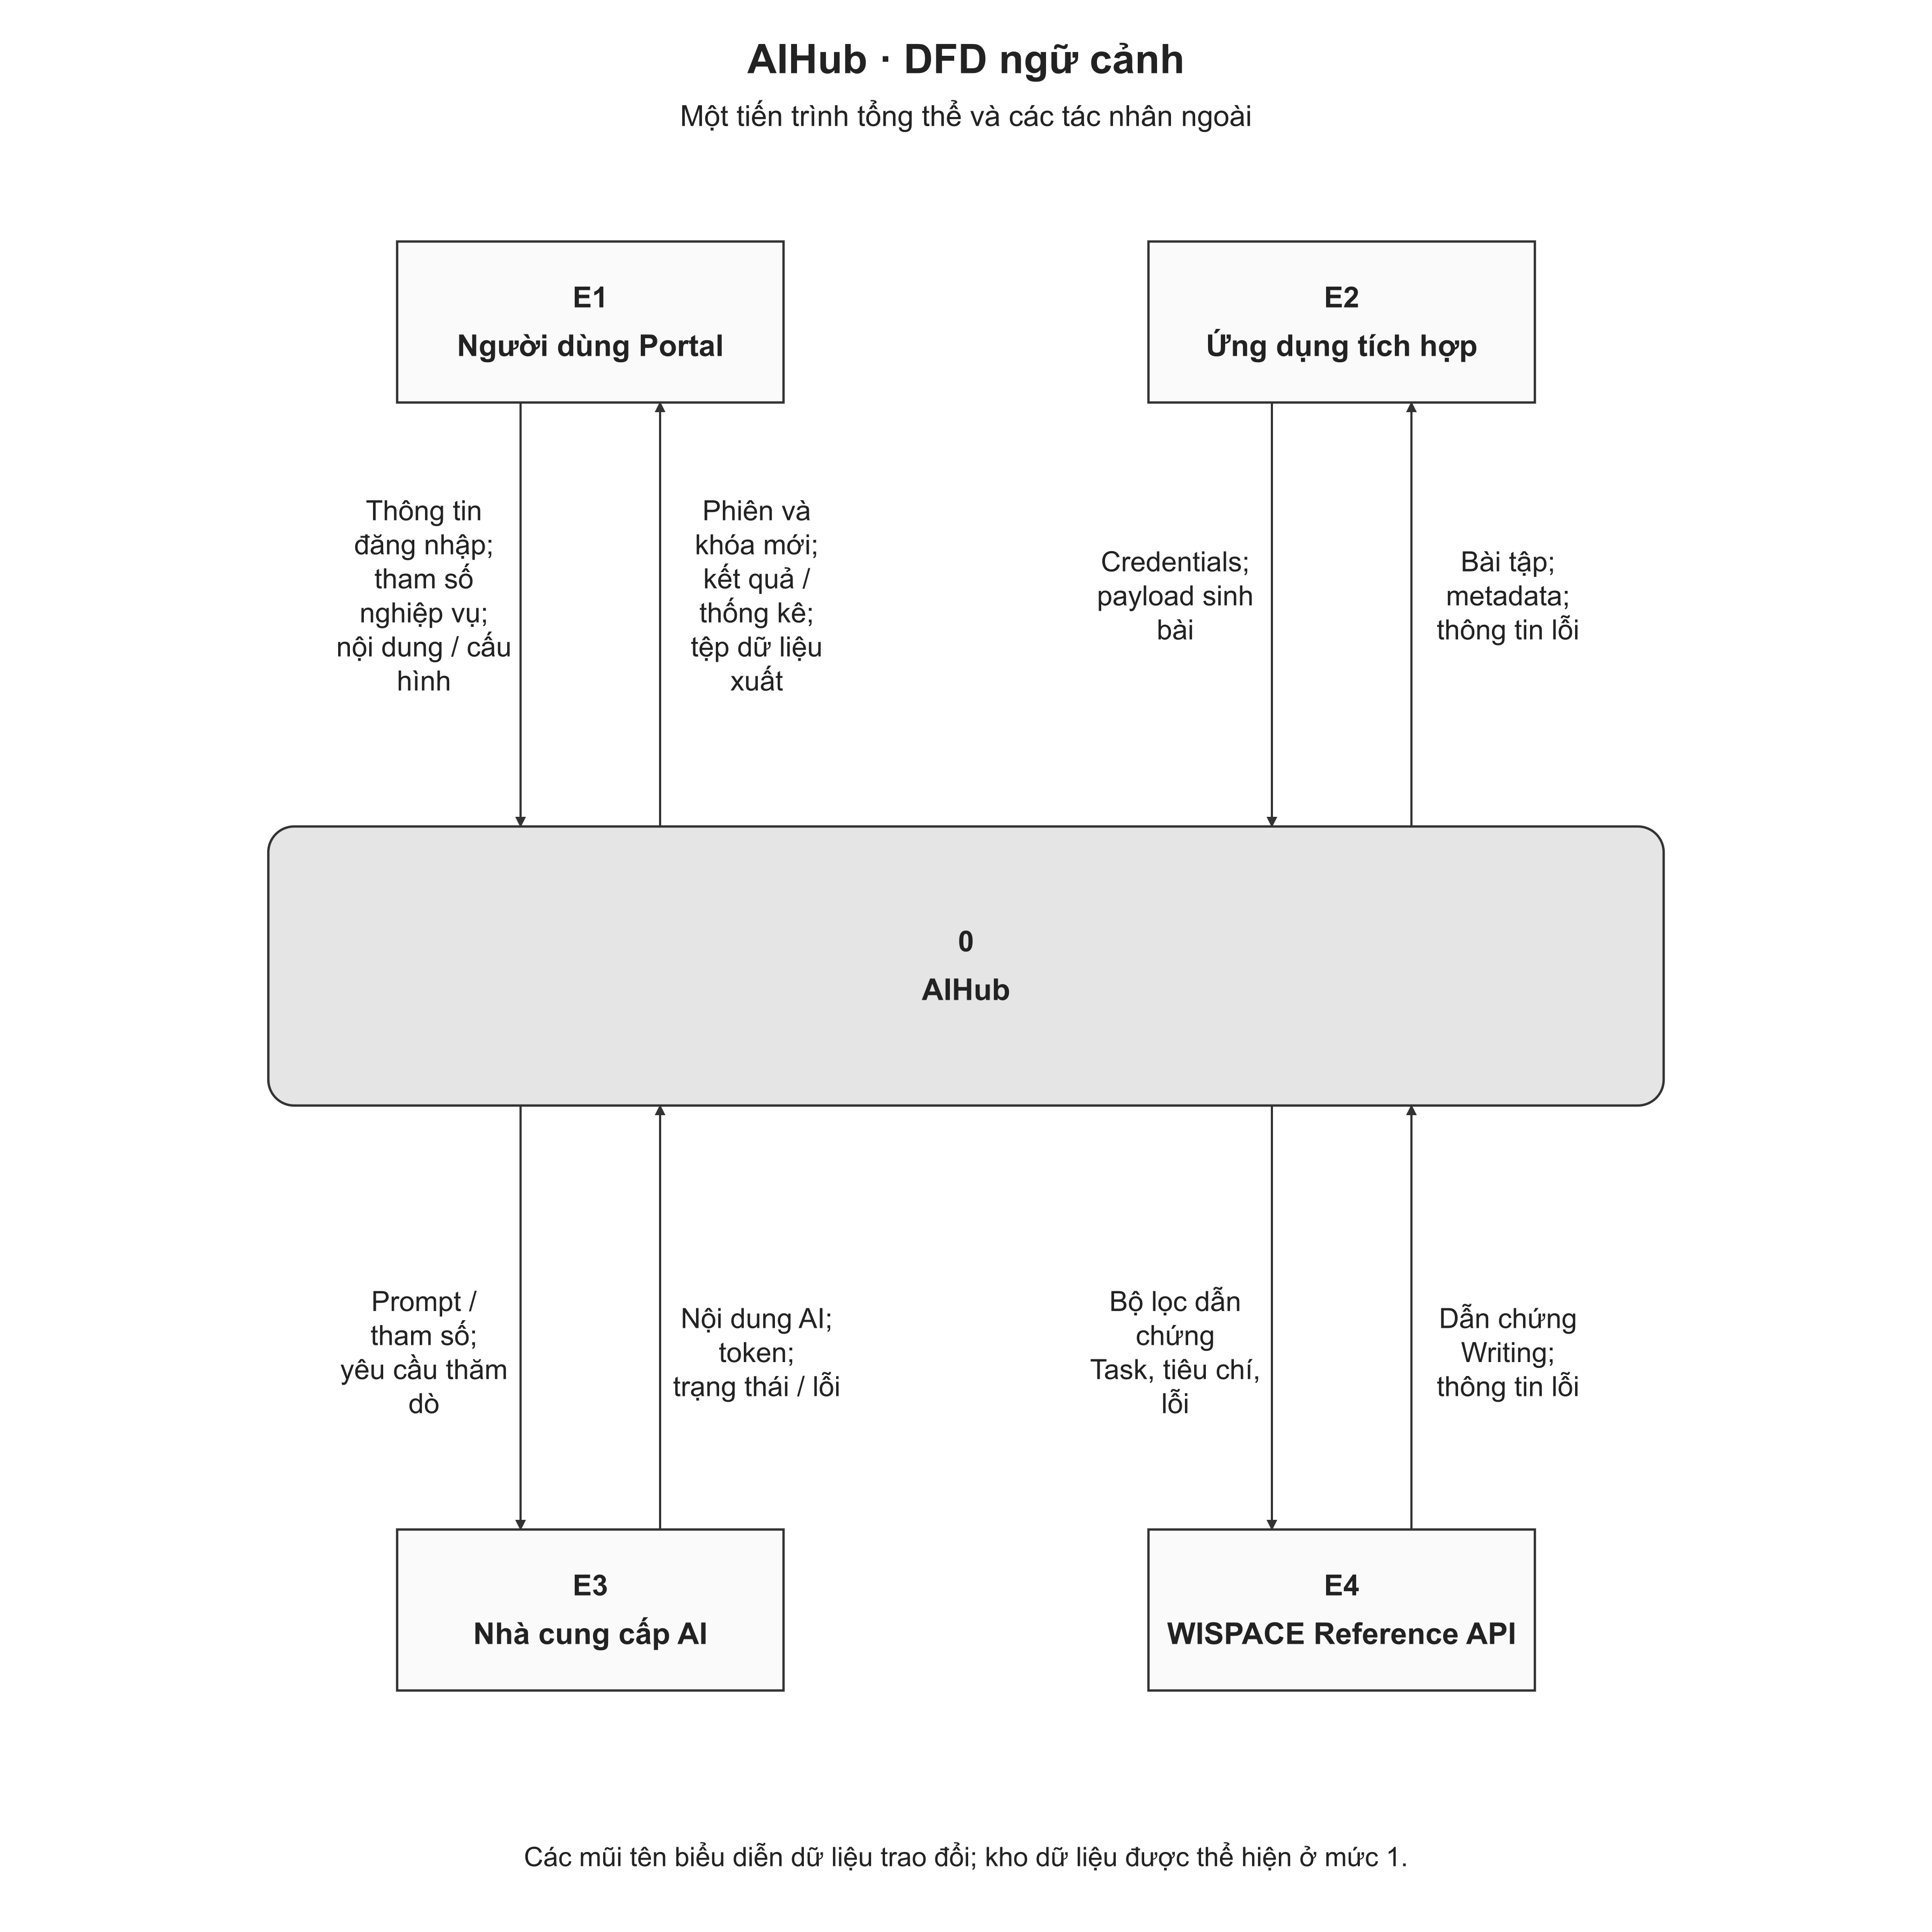
\includegraphics[width=\linewidth,height=0.78\textheight,keepaspectratio]{Images/DFD/AIHub/aihub_dfd_context.png}
\caption{DFD ngữ cảnh của AIHub}
\label{aihub:fig:dfd-context}
\end{figure}

\clearpage

\begin{longtable}{|p{0.22\linewidth}|p{0.72\linewidth}|}
\caption{Luồng dữ liệu biên của AIHub}\label{aihub:tab:dfd-boundary}\\
\hline
\textbf{Nguồn → Đích} & \textbf{Dữ liệu} \\
\hline
\endfirsthead
\hline
\textbf{Nguồn → Đích} & \textbf{Dữ liệu} \\
\hline
\endhead
E1 → 0 & Thông tin đăng nhập; tham số nghiệp vụ; nội dung / cấu hình \\
\hline
0 → E1 & Phiên và khóa mới; kết quả / thống kê; tệp dữ liệu xuất \\
\hline
E2 → 0 & Credentials; payload sinh bài \\
\hline
0 → E2 & Bài tập; metadata; thông tin lỗi \\
\hline
0 → E3 & Prompt / tham số; yêu cầu thăm dò \\
\hline
E3 → 0 & Nội dung AI; token; trạng thái / lỗi \\
\hline
0 → E4 & Bộ lọc dẫn chứng Task, tiêu chí, lỗi \\
\hline
E4 → 0 & Dẫn chứng Writing; thông tin lỗi \\
\hline
\end{longtable}


\paragraph{Sơ đồ mức 1.}

Để giữ nhãn và đường nối dễ đọc, cùng một sơ đồ mức 1 được trình bày thành hai phần. Các tác nhân và kho dữ liệu có cùng mã ở hai phần là cùng một đối tượng logic. Dữ liệu giữa các nhóm xử lý được trao đổi qua kho dùng chung, không phải các bản sao tách biệt.

\clearpage

\begin{figure}[H]
\centering
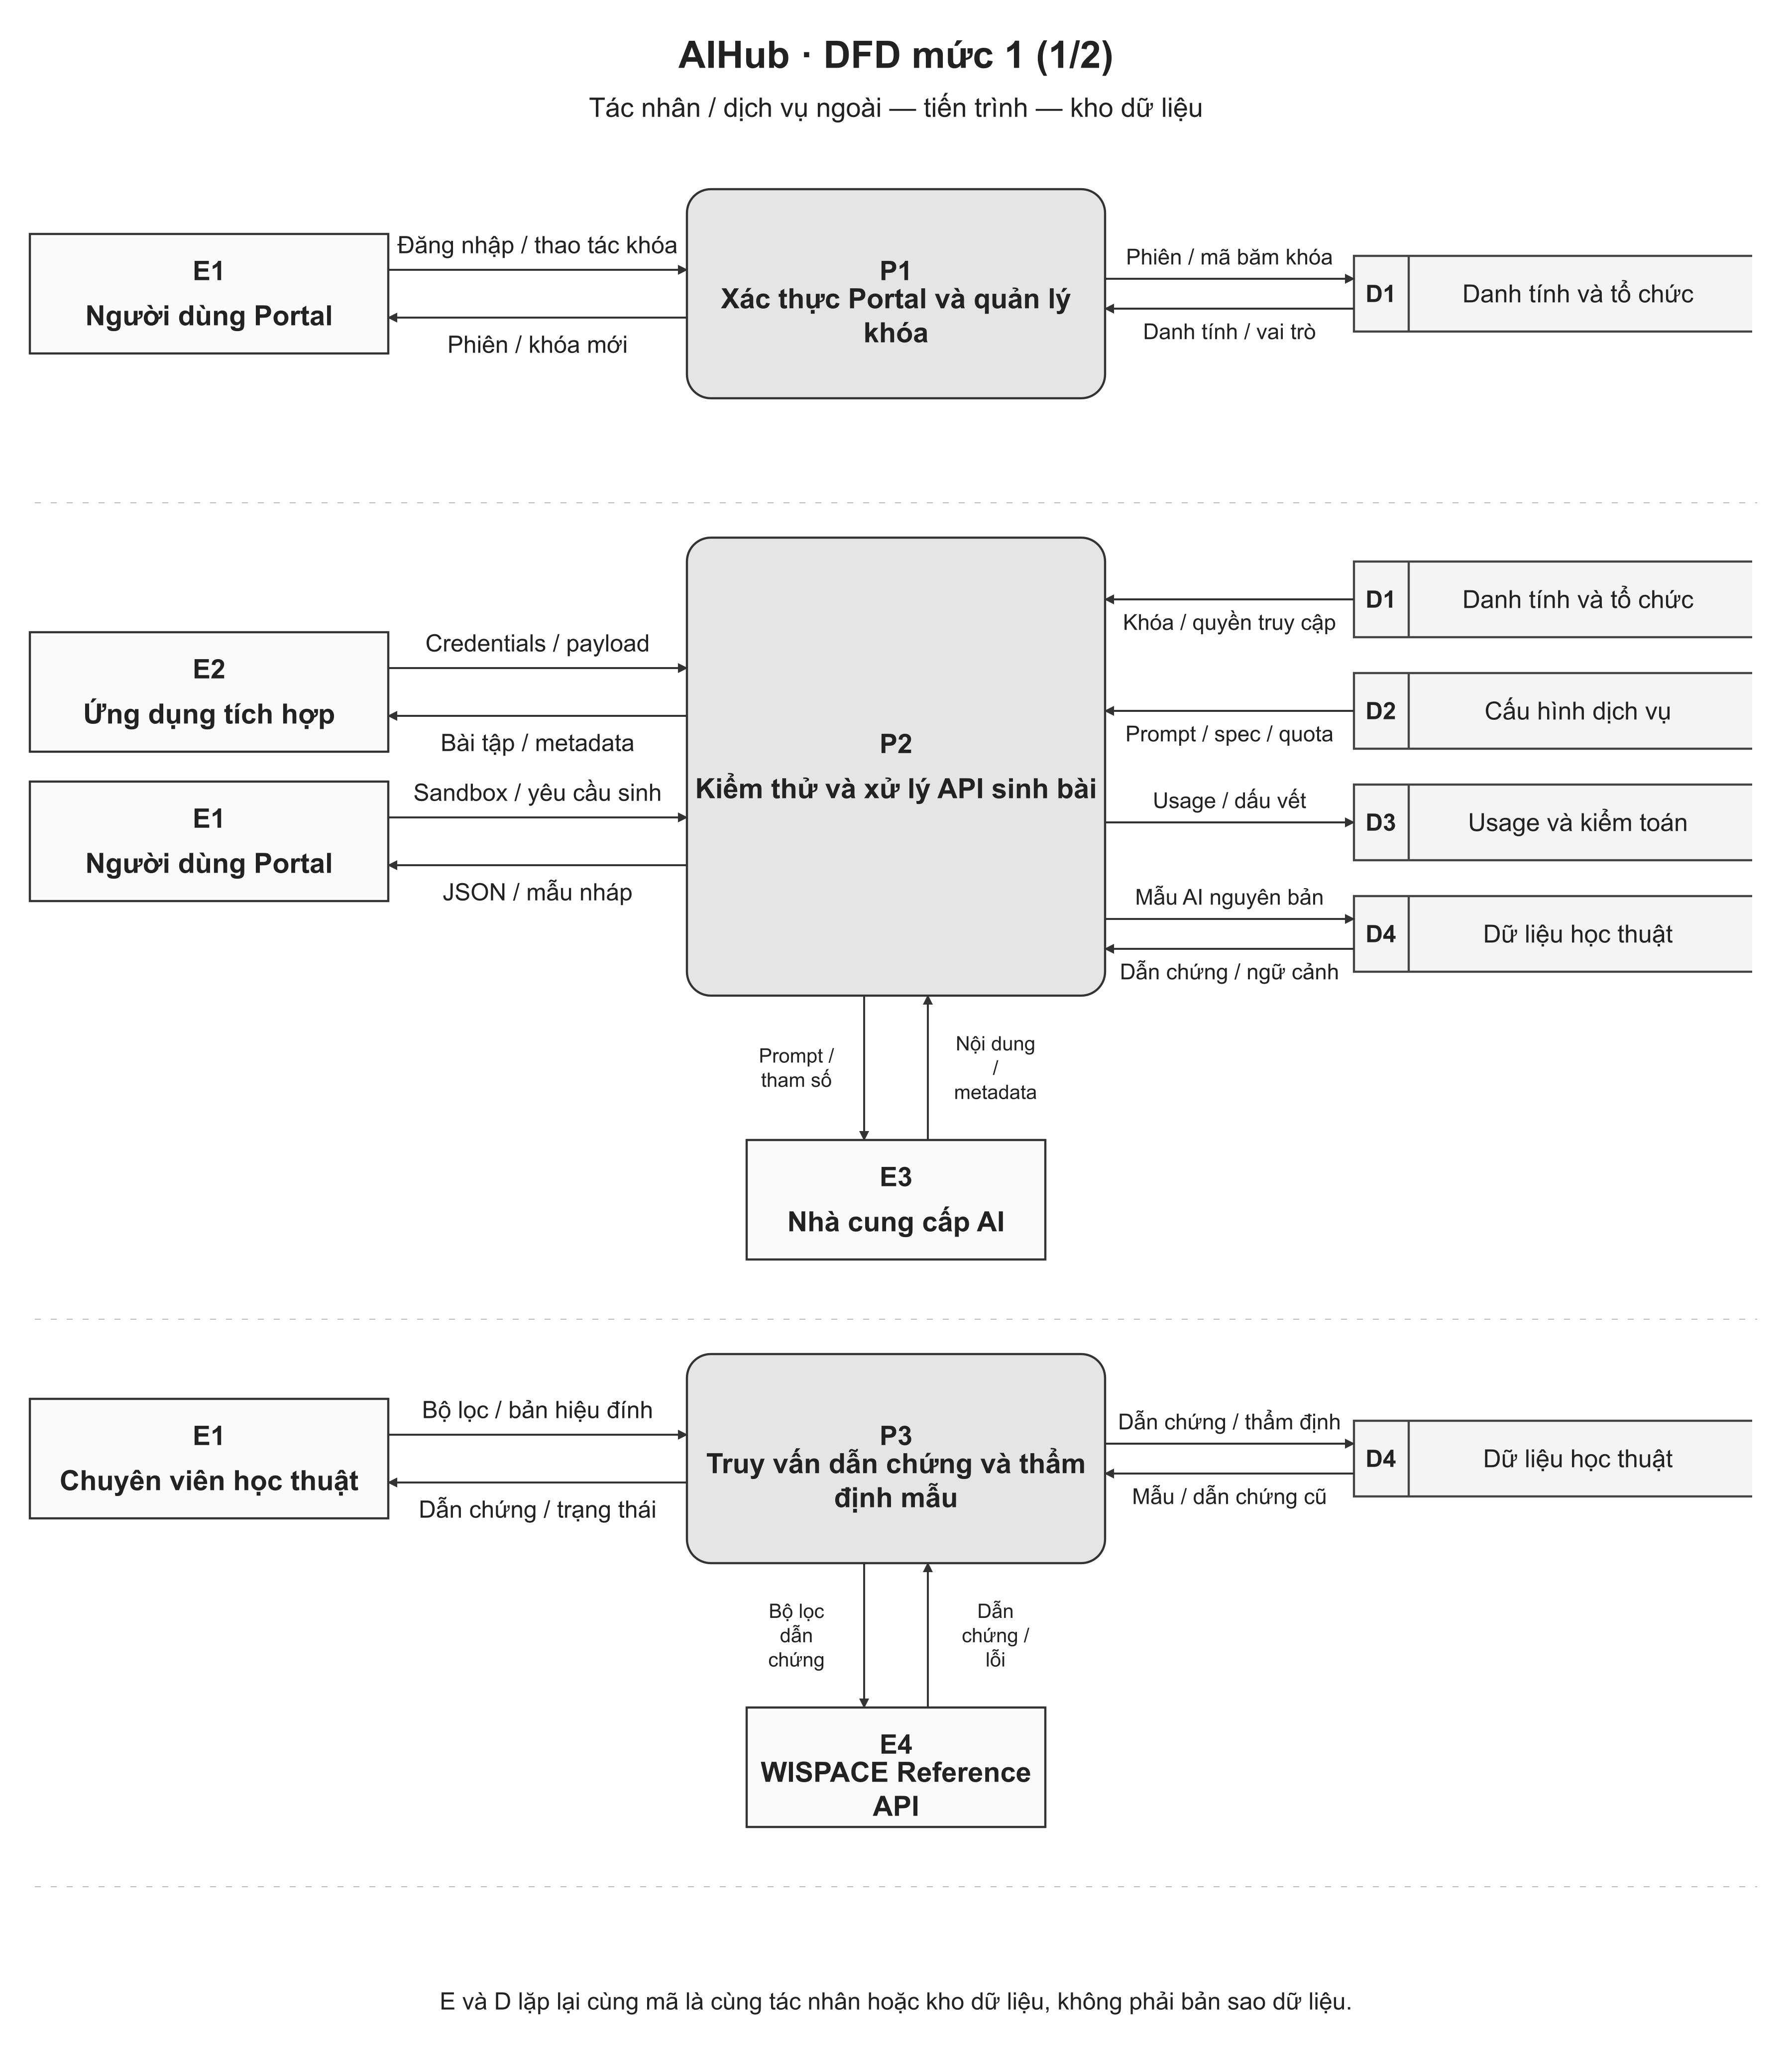
\includegraphics[width=\linewidth,height=0.78\textheight,keepaspectratio]{Images/DFD/AIHub/aihub_dfd_level1_1.png}
\caption{DFD mức 1 của AIHub: P1, P2, P3}
\label{aihub:fig:dfd-level1-1}
\end{figure}

\clearpage

\begin{figure}[H]
\centering
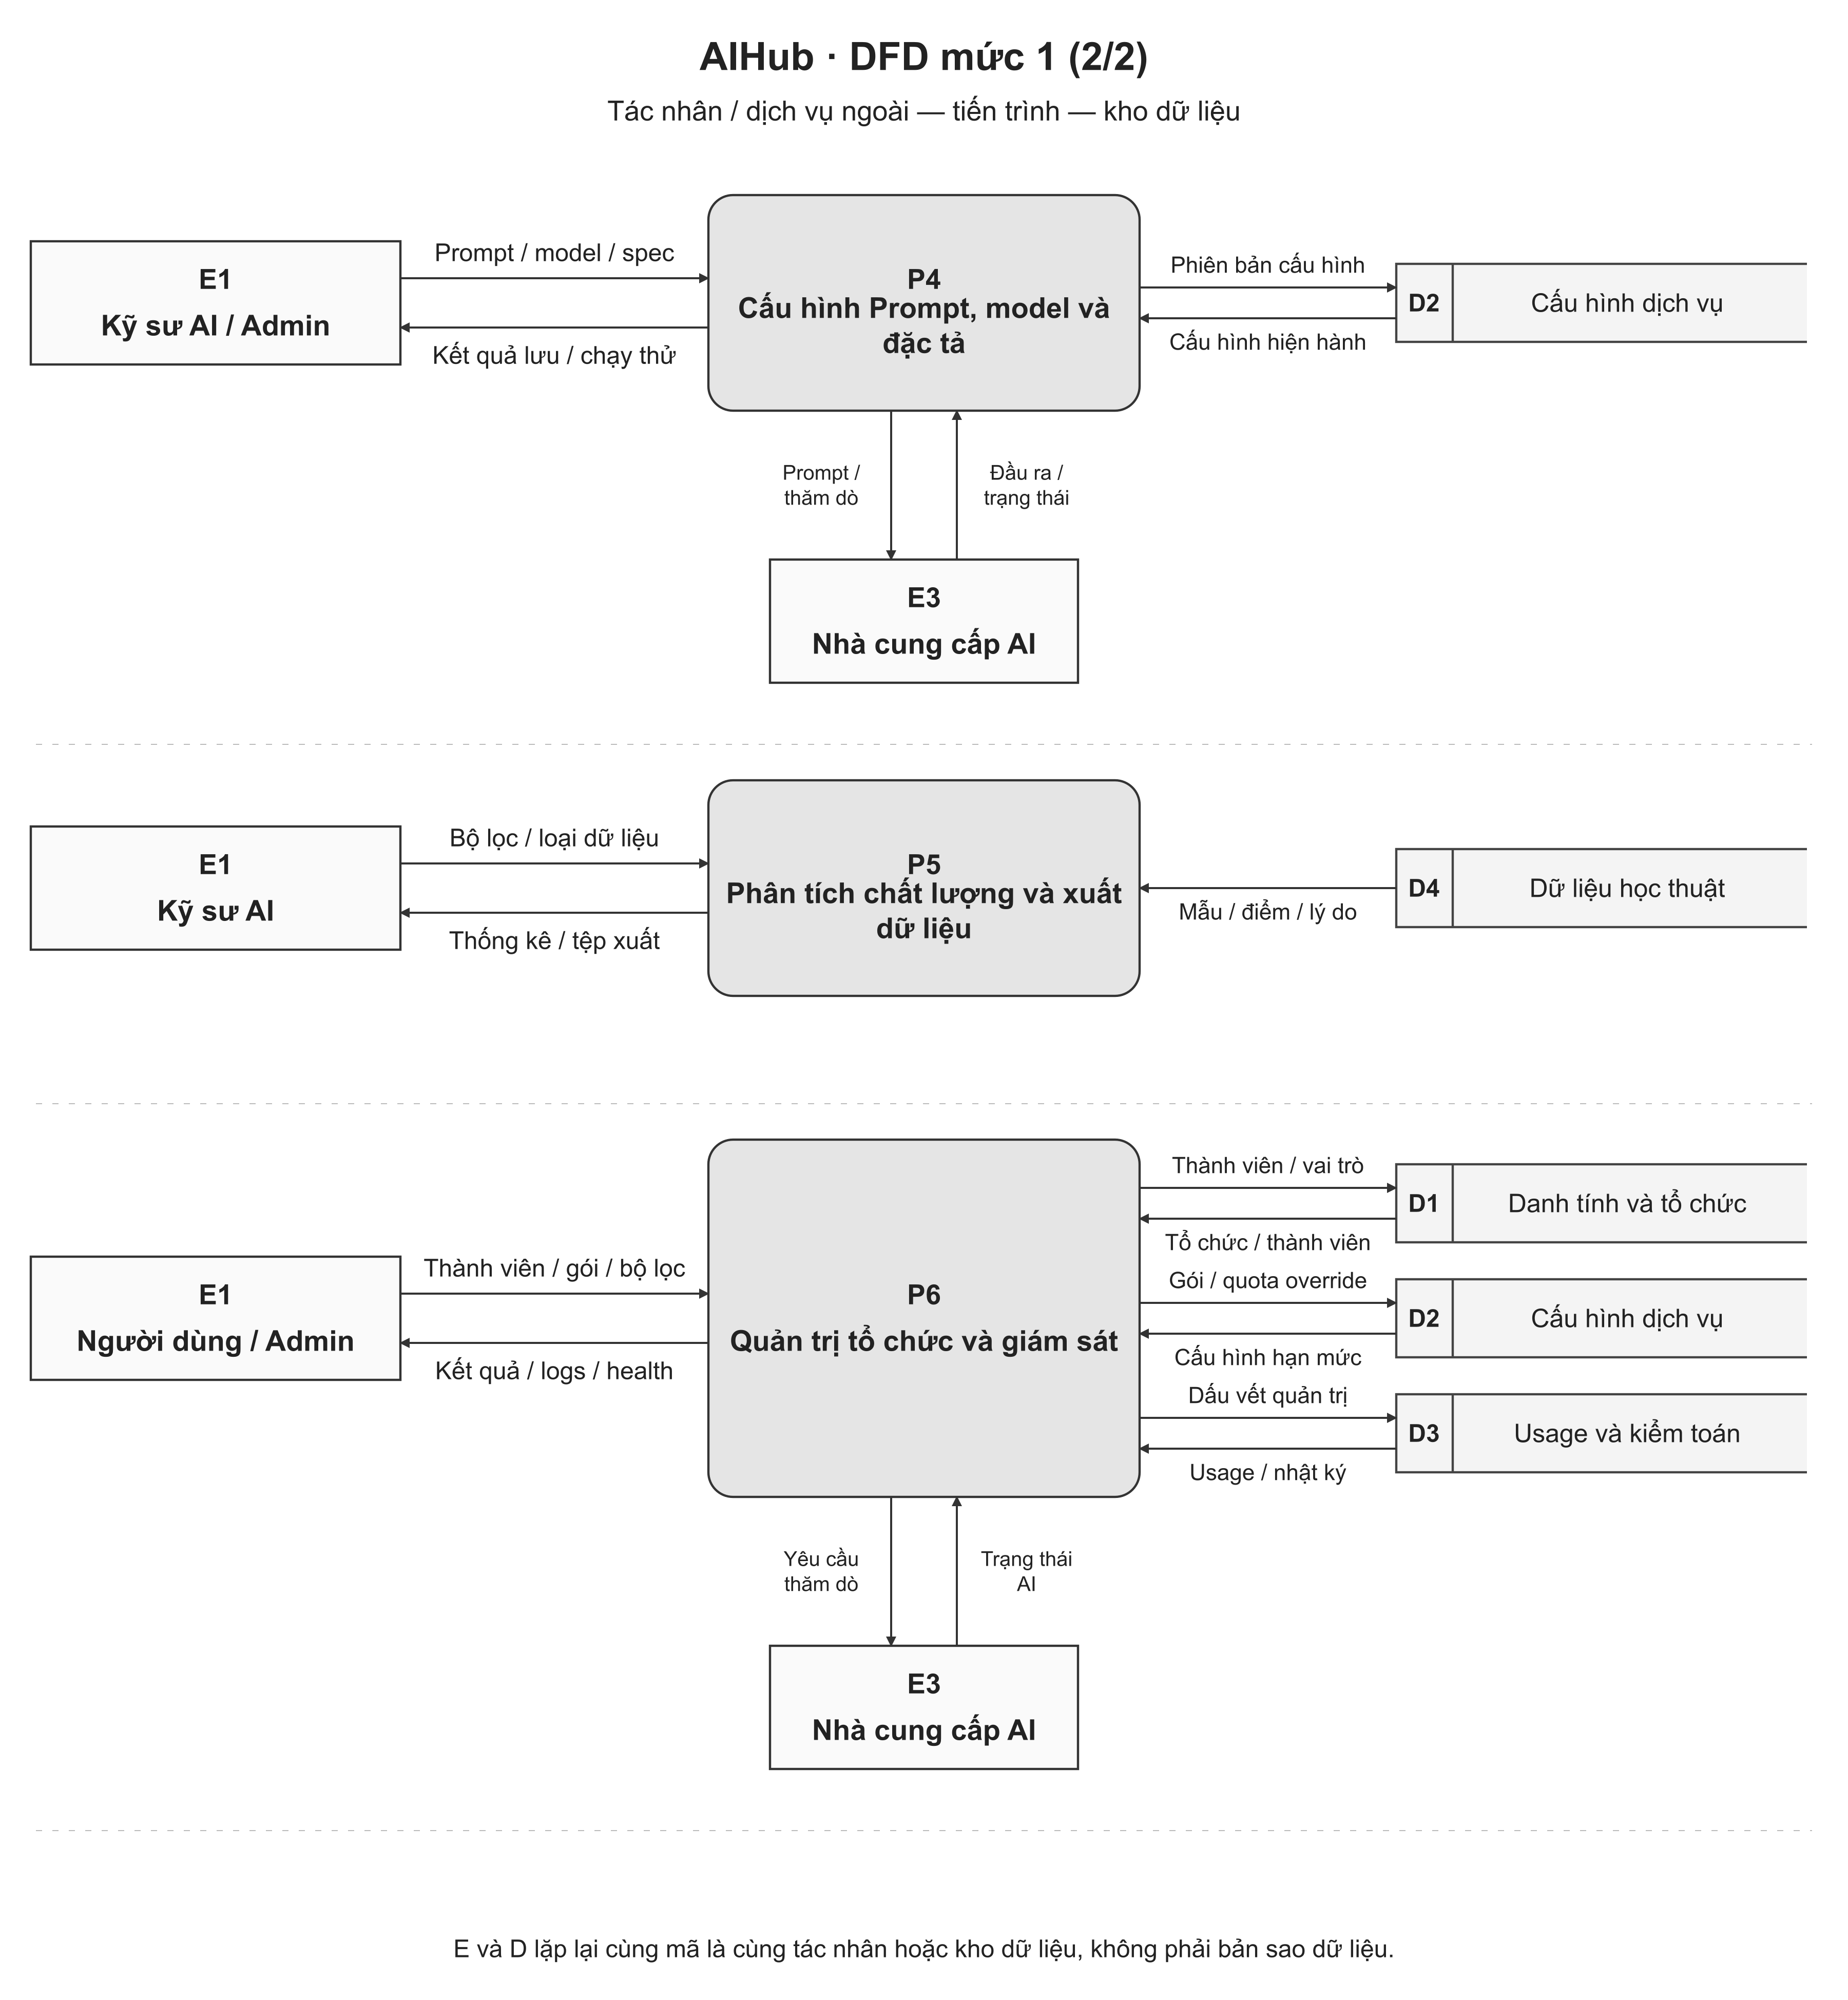
\includegraphics[width=\linewidth,height=0.78\textheight,keepaspectratio]{Images/DFD/AIHub/aihub_dfd_level1_2.png}
\caption{DFD mức 1 của AIHub: P4, P5, P6}
\label{aihub:fig:dfd-level1-2}
\end{figure}

\clearpage

\begin{longtable}{|p{0.22\linewidth}|p{0.72\linewidth}|}
\caption{Luồng dữ liệu mức 1 của AIHub}\label{aihub:tab:dfd-flows}\\
\hline
\textbf{Nguồn → Đích} & \textbf{Dữ liệu} \\
\hline
\endfirsthead
\hline
\textbf{Nguồn → Đích} & \textbf{Dữ liệu} \\
\hline
\endhead
E1 → P1 & Đăng nhập / thao tác khóa \\
\hline
P1 → E1 & Phiên / khóa mới \\
\hline
P1 → D1 & Phiên / mã băm khóa \\
\hline
D1 → P1 & Danh tính / vai trò \\
\hline
E2 → P2 & Credentials / payload \\
\hline
P2 → E2 & Bài tập / metadata \\
\hline
E1 → P2 & Sandbox / yêu cầu sinh \\
\hline
P2 → E1 & JSON / mẫu nháp \\
\hline
D1 → P2 & Khóa / quyền truy cập \\
\hline
D2 → P2 & Prompt / spec / quota \\
\hline
P2 → D3 & Usage / dấu vết \\
\hline
P2 → D4 & Mẫu AI nguyên bản \\
\hline
D4 → P2 & Dẫn chứng / ngữ cảnh \\
\hline
P2 → E3 & Prompt / tham số \\
\hline
E3 → P2 & Nội dung / metadata \\
\hline
E1 → P3 & Bộ lọc / bản hiệu đính \\
\hline
P3 → E1 & Dẫn chứng / trạng thái \\
\hline
P3 → D4 & Dẫn chứng / thẩm định \\
\hline
D4 → P3 & Mẫu / dẫn chứng cũ \\
\hline
P3 → E4 & Bộ lọc dẫn chứng \\
\hline
E4 → P3 & Dẫn chứng / lỗi \\
\hline
E1 → P4 & Prompt / model / spec \\
\hline
P4 → E1 & Kết quả lưu / chạy thử \\
\hline
P4 → D2 & Phiên bản cấu hình \\
\hline
D2 → P4 & Cấu hình hiện hành \\
\hline
P4 → E3 & Prompt / thăm dò \\
\hline
E3 → P4 & Đầu ra / trạng thái \\
\hline
E1 → P5 & Bộ lọc / loại dữ liệu \\
\hline
P5 → E1 & Thống kê / tệp xuất \\
\hline
D4 → P5 & Mẫu / điểm / lý do \\
\hline
E1 → P6 & Thành viên / gói / bộ lọc \\
\hline
P6 → E1 & Kết quả / logs / health \\
\hline
P6 → D1 & Thành viên / vai trò \\
\hline
D1 → P6 & Tổ chức / thành viên \\
\hline
P6 → D2 & Gói / quota override \\
\hline
D2 → P6 & Cấu hình hạn mức \\
\hline
P6 → D3 & Dấu vết quản trị \\
\hline
D3 → P6 & Usage / nhật ký \\
\hline
P6 → E3 & Yêu cầu thăm dò \\
\hline
E3 → P6 & Trạng thái AI \\
\hline
\end{longtable}


P3 lưu dẫn chứng vào D4 để P2 sử dụng khi sinh nội dung. Mẫu nguyên bản do P2 ghi vào D4 được P3 hiệu đính và thẩm định; P5 chỉ trích xuất dữ liệu phù hợp với loại tập huấn luyện được chọn. P2 và P6 cùng sử dụng D3 cho nhật ký và đối soát hạn mức. Sandbox của dịch vụ đối tác dùng dữ liệu mô phỏng trong P2, không phát sinh một lời gọi thật đến đối tác.

Deterministic Engine là thành phần dự phòng nội bộ của P2. Health check trong P6 kiểm tra kho dữ liệu nội bộ và nhận trạng thái từ nhà cung cấp AI; không xem PostgreSQL như một tác nhân ngoài.

Các luồng dữ liệu biên ở sơ đồ ngữ cảnh được phân bổ vào các tiến trình mức 1 tương ứng. Luồng đọc, ghi và phản hồi được thể hiện bằng các mũi tên riêng; sơ đồ không dùng điều kiện rẽ nhánh, nút bắt đầu hoặc kết thúc của activity diagram.


\subsection*{Kết chương}
Chương này đã phân tích các use-case, luồng hoạt động và luồng dữ liệu của Wispace Speaking và AIHub. Các mô hình xác định trách nhiệm của tác nhân, dữ liệu đầu vào, kết quả xử lý và các kho lưu trữ, làm cơ sở cho thiết kế và hiện thực hệ thống ở các chương tiếp theo.

% Chapter 7 source: maintained directly in LaTeX; diagrams have editable sources in Diagrams/.
\section{Thiết kế hệ thống}
\label{sec:system-design}
\setcounter{paragraph}{0}

Chương này trình bày thiết kế đề xuất cho hai hệ thống độc lập Wispace và AIHub, mỗi hệ thống có frontend React và backend .NET riêng. Wispace là sản phẩm chính, cung cấp môi trường luyện tập, thi thử và theo dõi tiến bộ IELTS cho người học. AIHub cung cấp cổng quản lý và khai thác API mô hình cho khách hàng doanh nghiệp, đồng thời có các công cụ nội bộ phục vụ đánh giá và cải thiện chất lượng mô hình.

Wispace sử dụng kiến trúc microservices theo các nhóm nghiệp vụ chính, hướng tới 1.000--10.000 người luyện tập hoặc thi đồng thời. AIHub giữ backend modular monolith riêng cho B2B và công cụ nội bộ. Các dịch vụ .NET của Wispace, hệ thống AIHub và Python FastAPI có hợp đồng tích hợp, quyền truy cập và tài nguyên được kiểm soát độc lập; Wispace gọi dịch vụ chấm trực tiếp qua Assessment, không qua cổng B2B.

Nội dung chương bao gồm kiến trúc tổng thể, phân chia module, thiết kế dữ liệu, xử lý âm thanh và chấm bài, quản lý API B2B, bảo mật, triển khai và giám sát. Thiết kế giữ giả định Scoring Model do Wispace tự huấn luyện; trọng tâm của chương là tích hợp và vận hành mô hình trong hệ thống. Các chỉ tiêu hiệu năng và độ chính xác là mục tiêu cần kiểm chứng khi hiện thực và thực nghiệm.

\subsection{Thiết kế hệ thống Wispace}

\subsubsection{Phạm vi, giao diện và kiến trúc}

Wispace là hệ thống học tập chính, tập trung vào luyện tập và thi thử Speaking IELTS. Thiết kế tách Core, Learning \& Exam, Assessment, Progress \& Reporting và AI Inference thành các đơn vị triển khai độc lập. Các dịch vụ nghiệp vụ dùng ASP.NET Core; AI Inference dùng Python FastAPI và Scoring Model tự huấn luyện. API Gateway định tuyến yêu cầu từ React; dịch vụ kiểm tra quyền nghiệp vụ tại ranh giới dữ liệu của mình. Mỗi dịch vụ có thể tổ chức nội bộ theo module, nhưng không dùng chung bảng dữ liệu với dịch vụ khác \cite{ch7_microservices,ch7_microservices_data}.

Phần thiết kế này bao gồm tài khoản, kho đề, kiểm duyệt, phiên luyện tập/thi thử, ghi âm, chấm điểm, báo cáo, lộ trình và quyền lợi gói học. Các chức năng AIHub được trình bày riêng tại Mục 7.2; việc dùng chung hạ tầng không làm hợp nhất hai phạm vi nghiệp vụ.

\paragraph*{Tổ chức frontend}

Frontend Wispace được tổ chức thành các nhóm màn hình tài khoản, kho đề, phòng luyện tập, phòng thi thử, kết quả, tiến bộ và quản trị nội dung. Các thành phần ghi âm, bộ đếm thời gian và trình phát audio được đóng gói để dùng chung giữa luyện tập và thi thử, nhưng quy tắc thao tác của hai chế độ được xử lý riêng.

Trong chế độ luyện tập, học viên có thể nghe lại và ghi lại trước khi nộp. Trong chế độ thi thử, hệ thống sử dụng trạng thái phiên trên backend để xác định Part, câu hỏi và thời hạn. Thời gian trên trình duyệt chỉ phục vụ hiển thị; mốc thời gian do backend lưu là căn cứ khi khôi phục phiên hoặc kết thúc bài.

Audio được thu theo khả năng trình duyệt. WebM/Opus và MP4/AAC là các đầu vào cần được hỗ trợ theo yêu cầu. FastAPI chuẩn hóa audio về định dạng đầu vào của Scoring Model; ứng dụng không giả định trình duyệt luôn ghi được đúng 16 kHz chỉ dựa vào tham số yêu cầu của MediaRecorder.

Để khôi phục khi mạng chập chờn, các đoạn ghi được lưu tạm trong IndexedDB và đánh số thứ tự. Mỗi đoạn có \texttt{upload\allowbreak{}Session\allowbreak{}Id}, \texttt{part\allowbreak{}Number} và checksum. Learning cấp URL tải lên có thời hạn để React gửi từng đoạn trực tiếp tới Object Storage; đường truyền audio không đi xuyên các API nghiệp vụ. Sau khi Learning xác minh object và checksum, frontend mới đánh dấu đoạn đó hoàn tất. Khi kết thúc, Learning kiểm tra manifest các đoạn, thứ tự và kích thước trước khi chấp nhận bài chấm.

\begin{figure}[H]
\centering
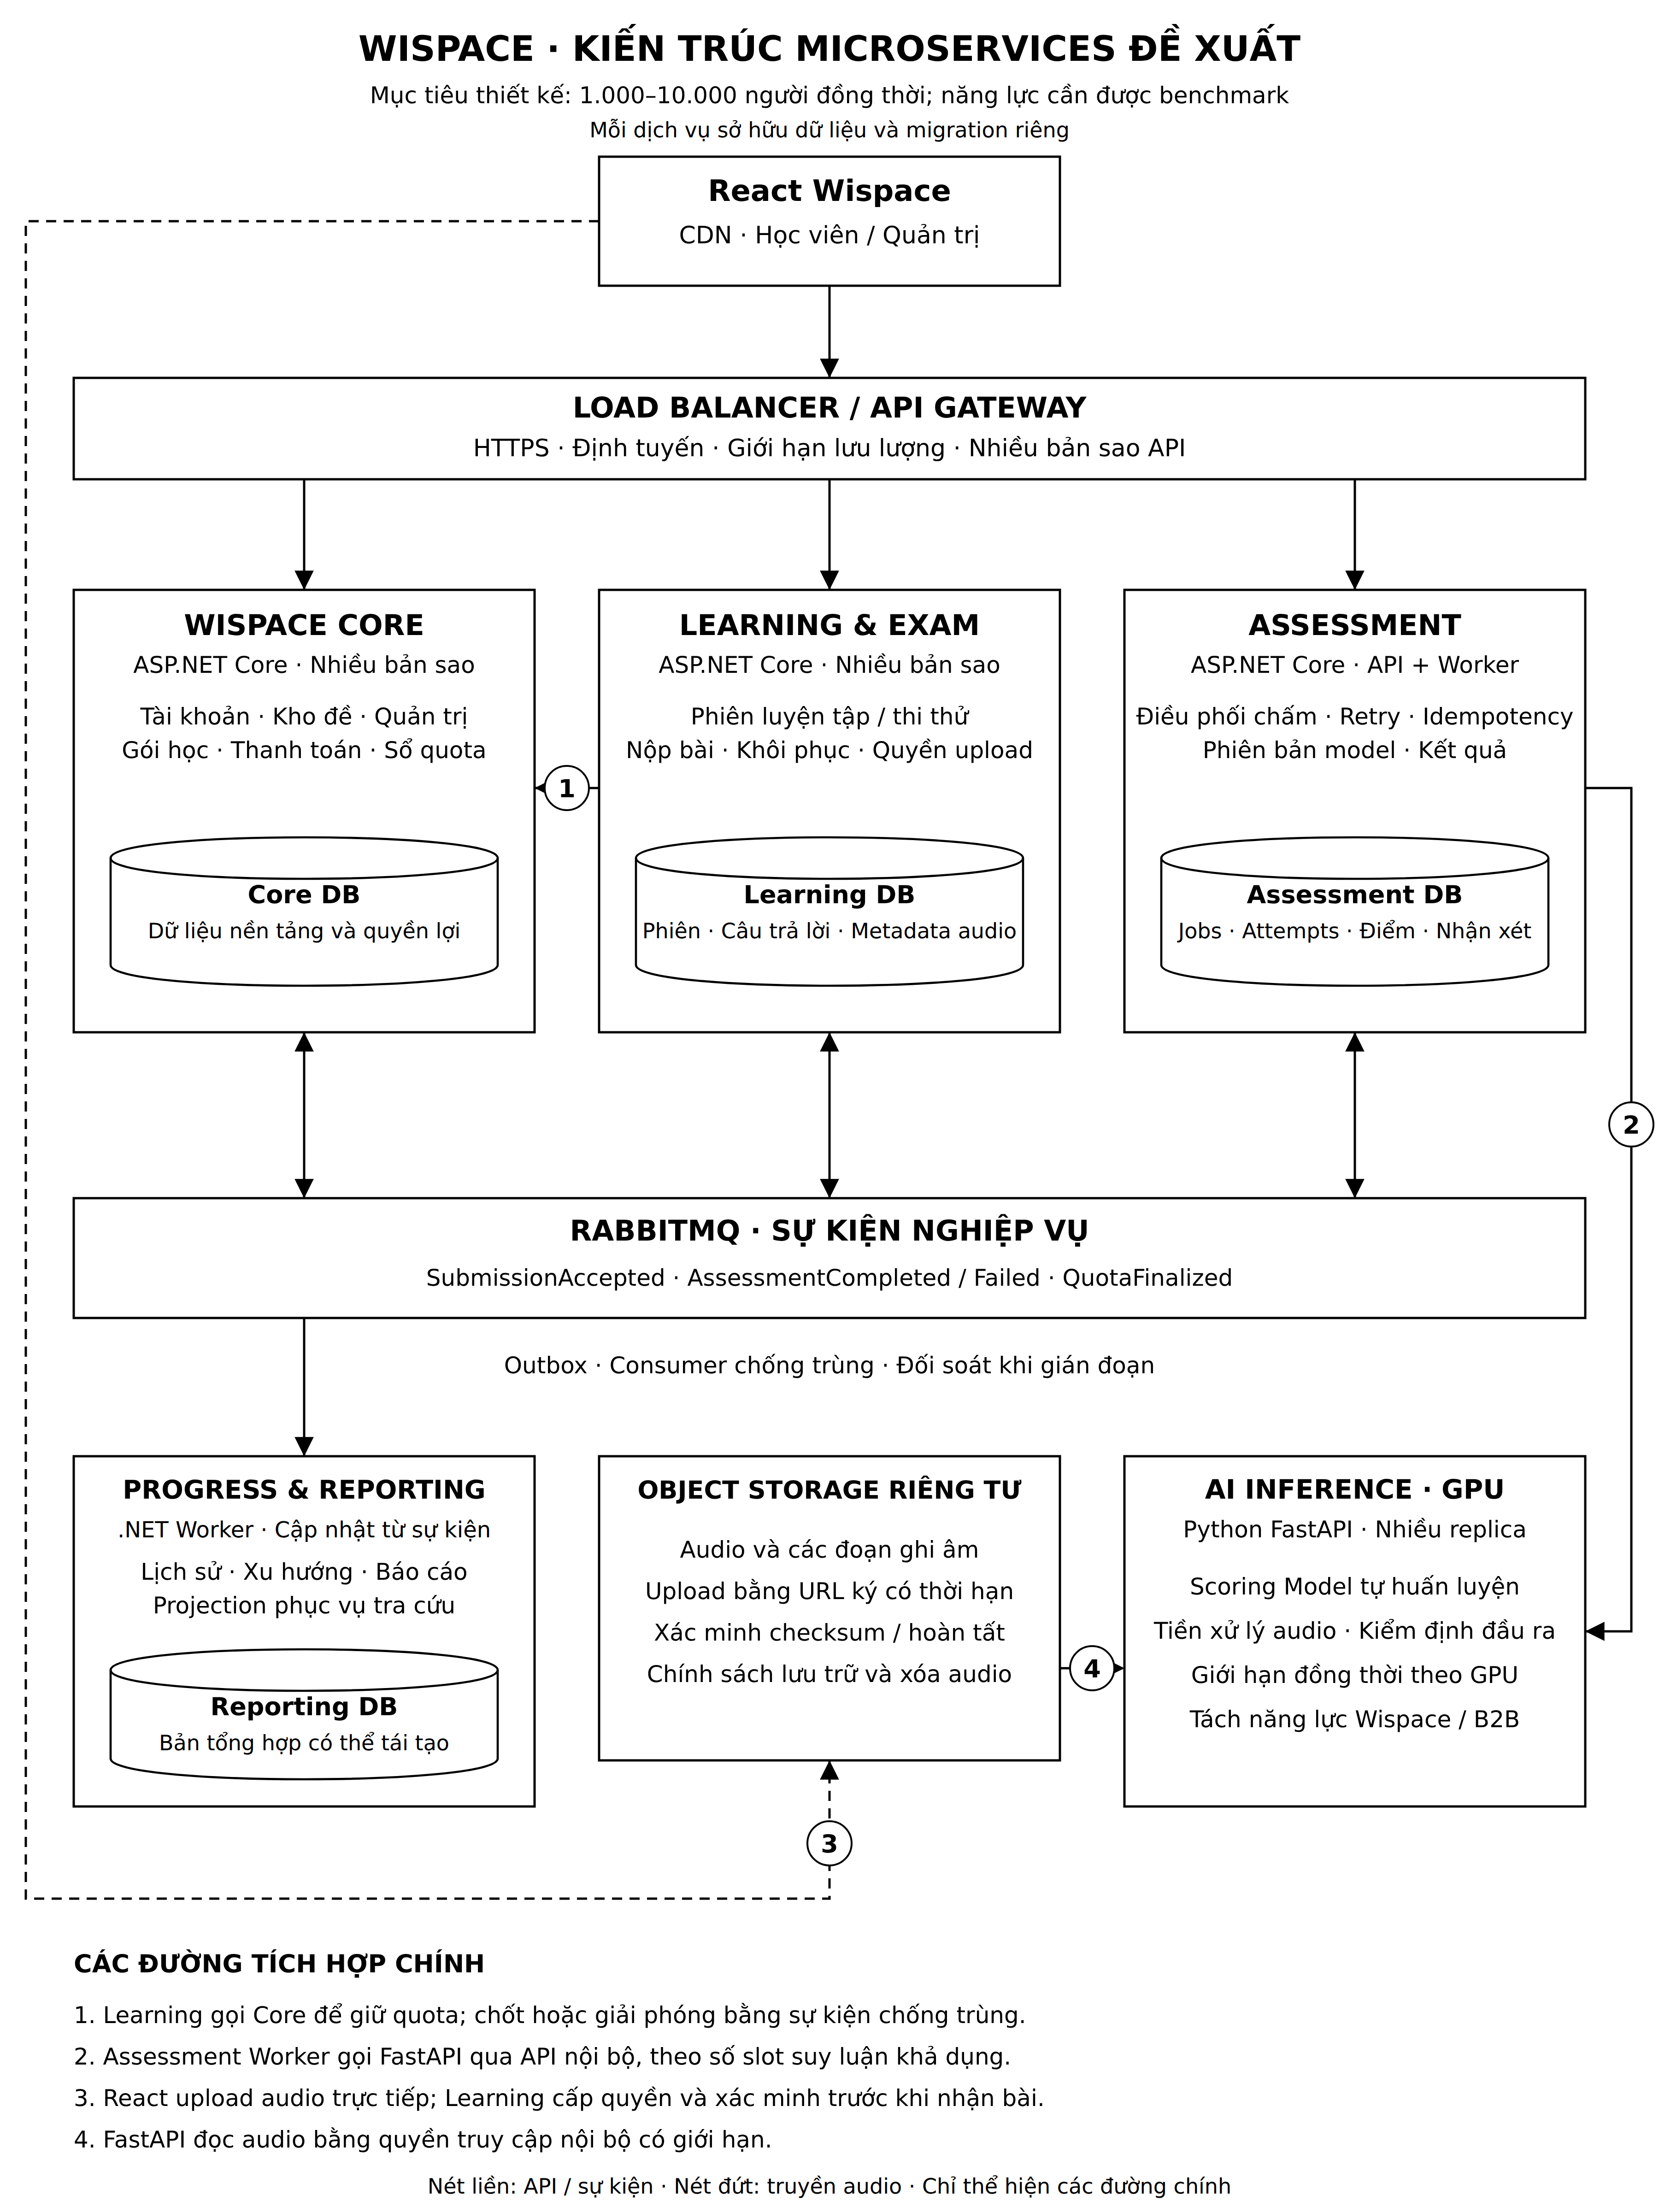
\includegraphics[width=\linewidth,height=.72\textheight,keepaspectratio]{Images/Design/wispace_microservices_proposal.png}
\caption{Kiến trúc microservices đề xuất cho Wispace}
\label{design:fig:wispace_architecture}
\end{figure}

\clearpage
\paragraph*{Ranh giới dịch vụ và quyền sở hữu dữ liệu}

\begingroup\small\setstretch{1.1}
\begin{longtable}{|>{\raggedright\arraybackslash}p{.25\linewidth}|>{\raggedright\arraybackslash}p{.65\linewidth}|}
\caption{Các dịch vụ của Wispace}\label{design:tab:1}\\\hline
\textbf{Dịch vụ} & \textbf{Trách nhiệm và dữ liệu sở hữu} \\\hline
\endfirsthead
\hline\textbf{Dịch vụ} & \textbf{Trách nhiệm và dữ liệu sở hữu} \\\hline\endhead
Core & Tài khoản, phiên đăng nhập, kho đề, kiểm duyệt, gói học, thanh toán và sổ quota. Core DB lưu danh tính, đề có phiên bản, giao dịch và bút toán quyền lợi. \\\hline
Learning \& Exam & Phiên học/thi, thời hạn máy chủ, câu trả lời, manifest audio và tiếp nhận bài nộp. Learning DB lưu trạng thái phiên và submission; dịch vụ cấp quyền upload sau khi kiểm tra chủ sở hữu. \\\hline
Assessment & API trạng thái/kết quả và Worker điều phối chấm. Assessment DB sở hữu job, attempt, lease, phiên bản mô hình, kết quả, báo cáo thi thử và liên kết chia sẻ. \\\hline
Progress \& Reporting & API đọc và Worker tổng hợp lịch sử, xu hướng, lỗi lặp và roadmap. Reporting DB là bản tổng hợp từ sự kiện, có thể tái tạo từ nguồn dữ liệu nghiệp vụ. \\\hline
AI Inference & FastAPI nạp Scoring Model, chuẩn hóa audio, suy luận và kiểm định đầu ra. Không sửa dữ liệu bài làm hoặc sổ quota; kết quả được Assessment công nhận và lưu. \\\hline
\end{longtable}\endgroup

Không tách một service cho từng bảng CRUD. Core giữ các nghiệp vụ nền tảng trong một lõi có module; phiên thi, điều phối chấm, báo cáo và suy luận được tách để mở rộng và phát hành độc lập. Các dịch vụ gọi Core qua hợp đồng API cho nghiệp vụ giữ quota, không truy vấn trực tiếp Core DB. Nội dung đề được Core cung cấp với phiên bản; Learning lưu snapshot câu hỏi của phiên để thay đổi kho đề không sửa lịch sử thi.

\paragraph*{Mục tiêu tải và nguyên tắc cô lập}

Mức 1.000--10.000 người đồng thời là mục tiêu thiết kế cần kiểm chứng, không phải kết quả đo. Phải phân biệt người đang mở trang, đang ghi âm, đang upload, bài nộp mỗi giây và lượt suy luận đang chạy. Nếu 10.000 người đều tải một đoạn audio mỗi 5 giây, lưu lượng trung bình riêng đường upload là khoảng 2.000 yêu cầu/giây; đây là kịch bản tính toán, chưa phải benchmark. Thiết kế sử dụng upload trực tiếp, nhiều bản sao API, cache nội dung đề và hàng đợi có giới hạn để phân tách các nhóm tải.

Luồng chuyển câu trong thi thử không đợi chấm câu trước. Learning quyết định câu và thời hạn từ trạng thái phiên; TTS được chuẩn bị hoặc cache trước. Lỗi Assessment hoặc GPU không được làm mất các đoạn audio đã xác nhận hoặc ngăn tiếp tục phiên thi đủ điều kiện. Trạng thái phiên cần lưu bền vững, không chỉ nằm trong bộ nhớ của một replica.

\subsubsection{Thiết kế dữ liệu và audio}

\begin{figure}[H]
\centering
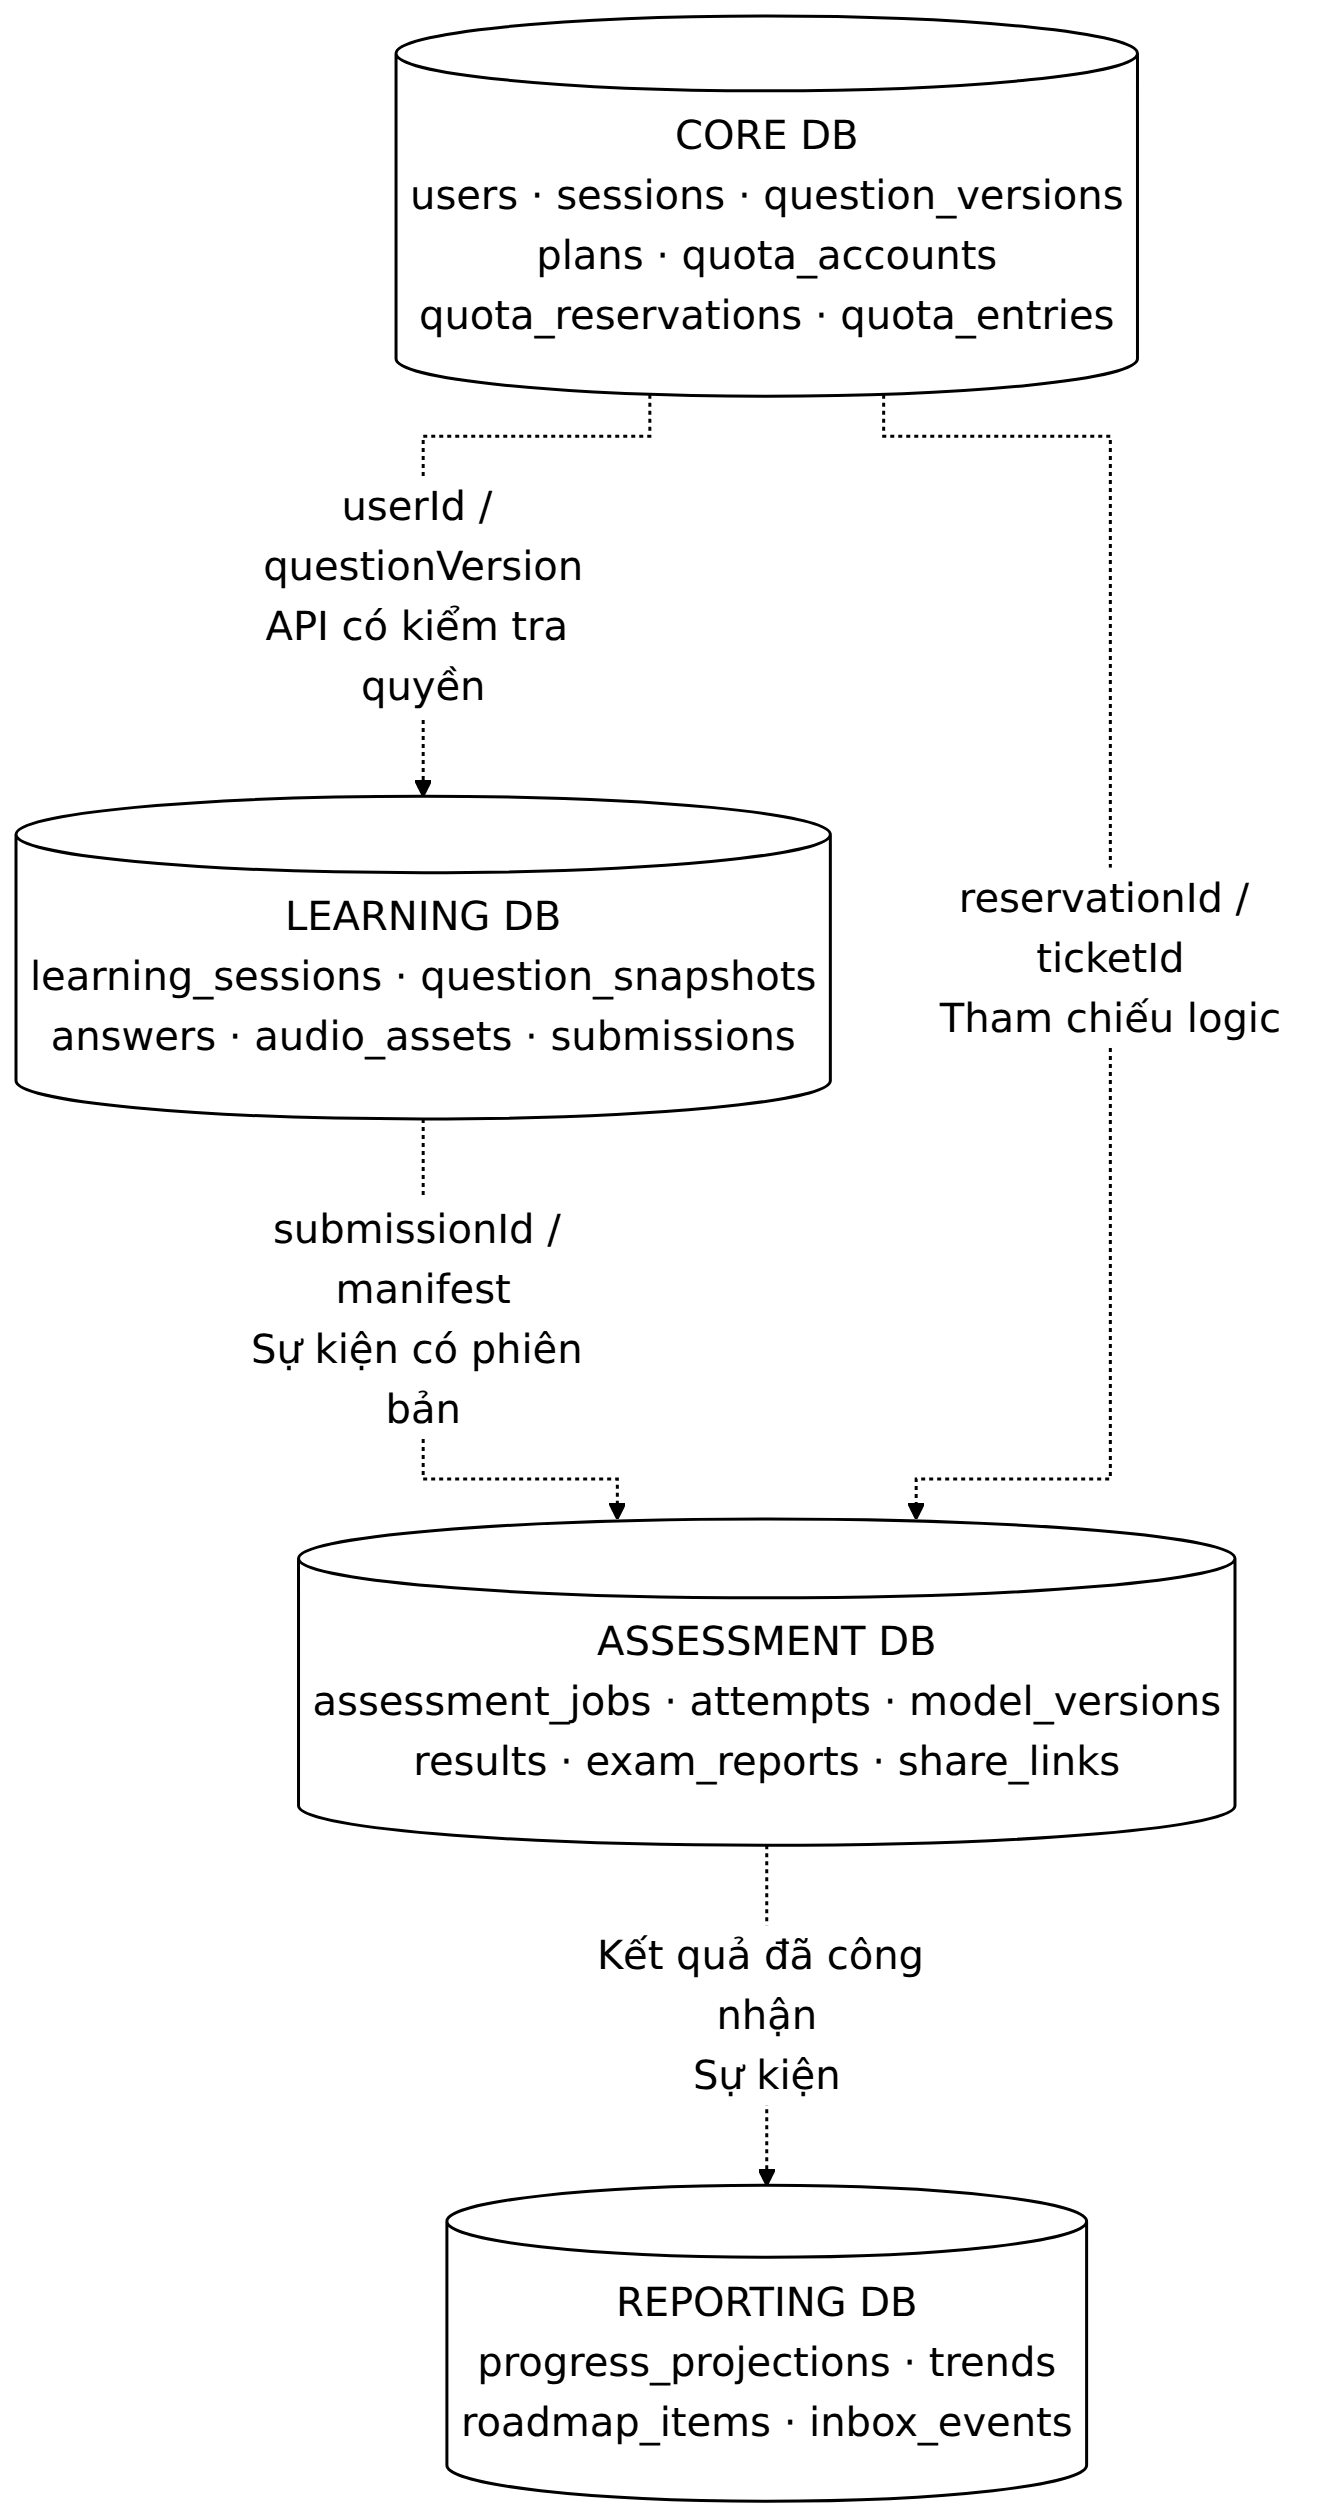
\includegraphics[width=\linewidth,height=.72\textheight,keepaspectratio]{Images/Design/wispace_data.png}
\caption{Phân tách dữ liệu theo dịch vụ Wispace}
\label{design:fig:wispace_data}
\end{figure}

Sơ đồ thể hiện quyền sở hữu dữ liệu theo dịch vụ. Mỗi dịch vụ nghiệp vụ có PostgreSQL database, credentials và migration riêng; các database có thể đặt cùng cụm vật lý khi năng lực cho phép. Các mã người học, phiên, submission và reservation được truyền qua API/sự kiện. Liên kết xuyên dịch vụ là định danh logic, không phải khóa ngoại hoặc transaction xuyên database. Một submission có thể có nhiều job do chấm lại; mỗi job có nhiều attempt và tối đa một kết quả cuối cùng được công nhận. Reporting chỉ lưu bản tổng hợp, không trở thành nguồn quyết định quota hoặc trạng thái thi.

PostgreSQL lưu metadata, object key, checksum, kích thước và trạng thái; nội dung audio nằm trong bucket riêng tư. Object key được backend tạo theo định danh nội bộ và không sử dụng tên tệp do người dùng gửi làm đường dẫn lưu trữ.

Learning chỉ cấp quyền tải lên cho object thuộc phiên và câu trả lời mà người dùng sở hữu. Việc hoàn tất upload phải kiểm tra object thực tế, checksum và giới hạn kích thước trước khi đánh dấu \texttt{Uploaded}. Link tải lên không đồng nghĩa tệp đã được chấp nhận để chấm.

Khi người dùng nghe lại bài, backend kiểm tra quyền và cấp URL đọc có thời hạn tối đa 10 phút theo yêu cầu đã xác định. URL ký trước là quyền truy cập tạm thời vào đúng object; hệ thống không ghi toàn bộ URL vào log \cite{ch7_s3_presigned}. Với Assessment Worker, quyền đọc object được lấy từ dịch vụ Learning hoặc tài khoản dịch vụ có phạm vi tương ứng tại thời điểm bắt đầu từng attempt, tránh hết hạn khi chờ hàng đợi. Message chỉ mang object key và metadata đã xác minh; không chứa audio hoặc URL ký dài hạn.

Tác vụ định kỳ xóa audio sau 180 ngày theo chính sách ở Chương 5, cập nhật trạng thái tệp và giữ transcript, điểm cùng các dữ liệu được phép lưu. Yêu cầu xóa trước hạn cũng được đưa vào quy trình có thể thử lại. Dữ liệu trong bản sao lưu tuân theo vòng đời backup được công bố; thời điểm xóa khỏi hệ thống hoạt động không được mô tả như xóa tức thời khỏi mọi bản sao lưu.

\subsubsection{Thiết kế tích hợp AI và xử lý bài làm}

\paragraph*{Tiếp nhận bài, quota và nhất quán xuyên dịch vụ}

Learning tạo submission ở trạng thái chờ, gắn khóa chống trùng và tham chiếu audio đã xác minh. Learning gọi Core để giữ quota bằng cùng mã nghiệp vụ; Core kiểm tra quyền lợi và ghi reservation trong transaction của Core DB. Khi được xác nhận, Learning ghi trạng thái Accepted và sự kiện \texttt{Submission\allowbreak{}Accepted} vào outbox trong cùng transaction của Learning DB, sau đó trả \texttt{202 Accepted} cùng \texttt{submission\allowbreak{}Id} và URL trạng thái. Assessment nhận sự kiện, tạo job và outbox xử lý trong transaction của Assessment DB; job được ràng buộc duy nhất theo submission và loại lần chấm.

Đây là chuỗi giao dịch cục bộ có bù và đối soát, không phải một transaction ACID bao trùm bốn database. Nếu lời gọi giữ quota timeout, Learning tra cứu kết quả bằng cùng mã nghiệp vụ trước khi tiếp tục hoặc hủy. Nếu Core đã giữ quota nhưng Learning chưa Accepted, tác vụ đối soát phục hồi hoặc dùng cập nhật có điều kiện để xác nhận hủy submission tại Learning trước khi Core giải phóng phần giữ đúng một lần. Khi trạng thái phía Learning chưa xác định, không tự hoàn quota chỉ vì timeout. Submission đã Accepted phải được giao nhận lại từ outbox hoặc đối soát cho tới khi Assessment ghi nhận; việc hết hạn không được âm thầm xóa bài đã nhận.

\begin{figure}[H]\centering
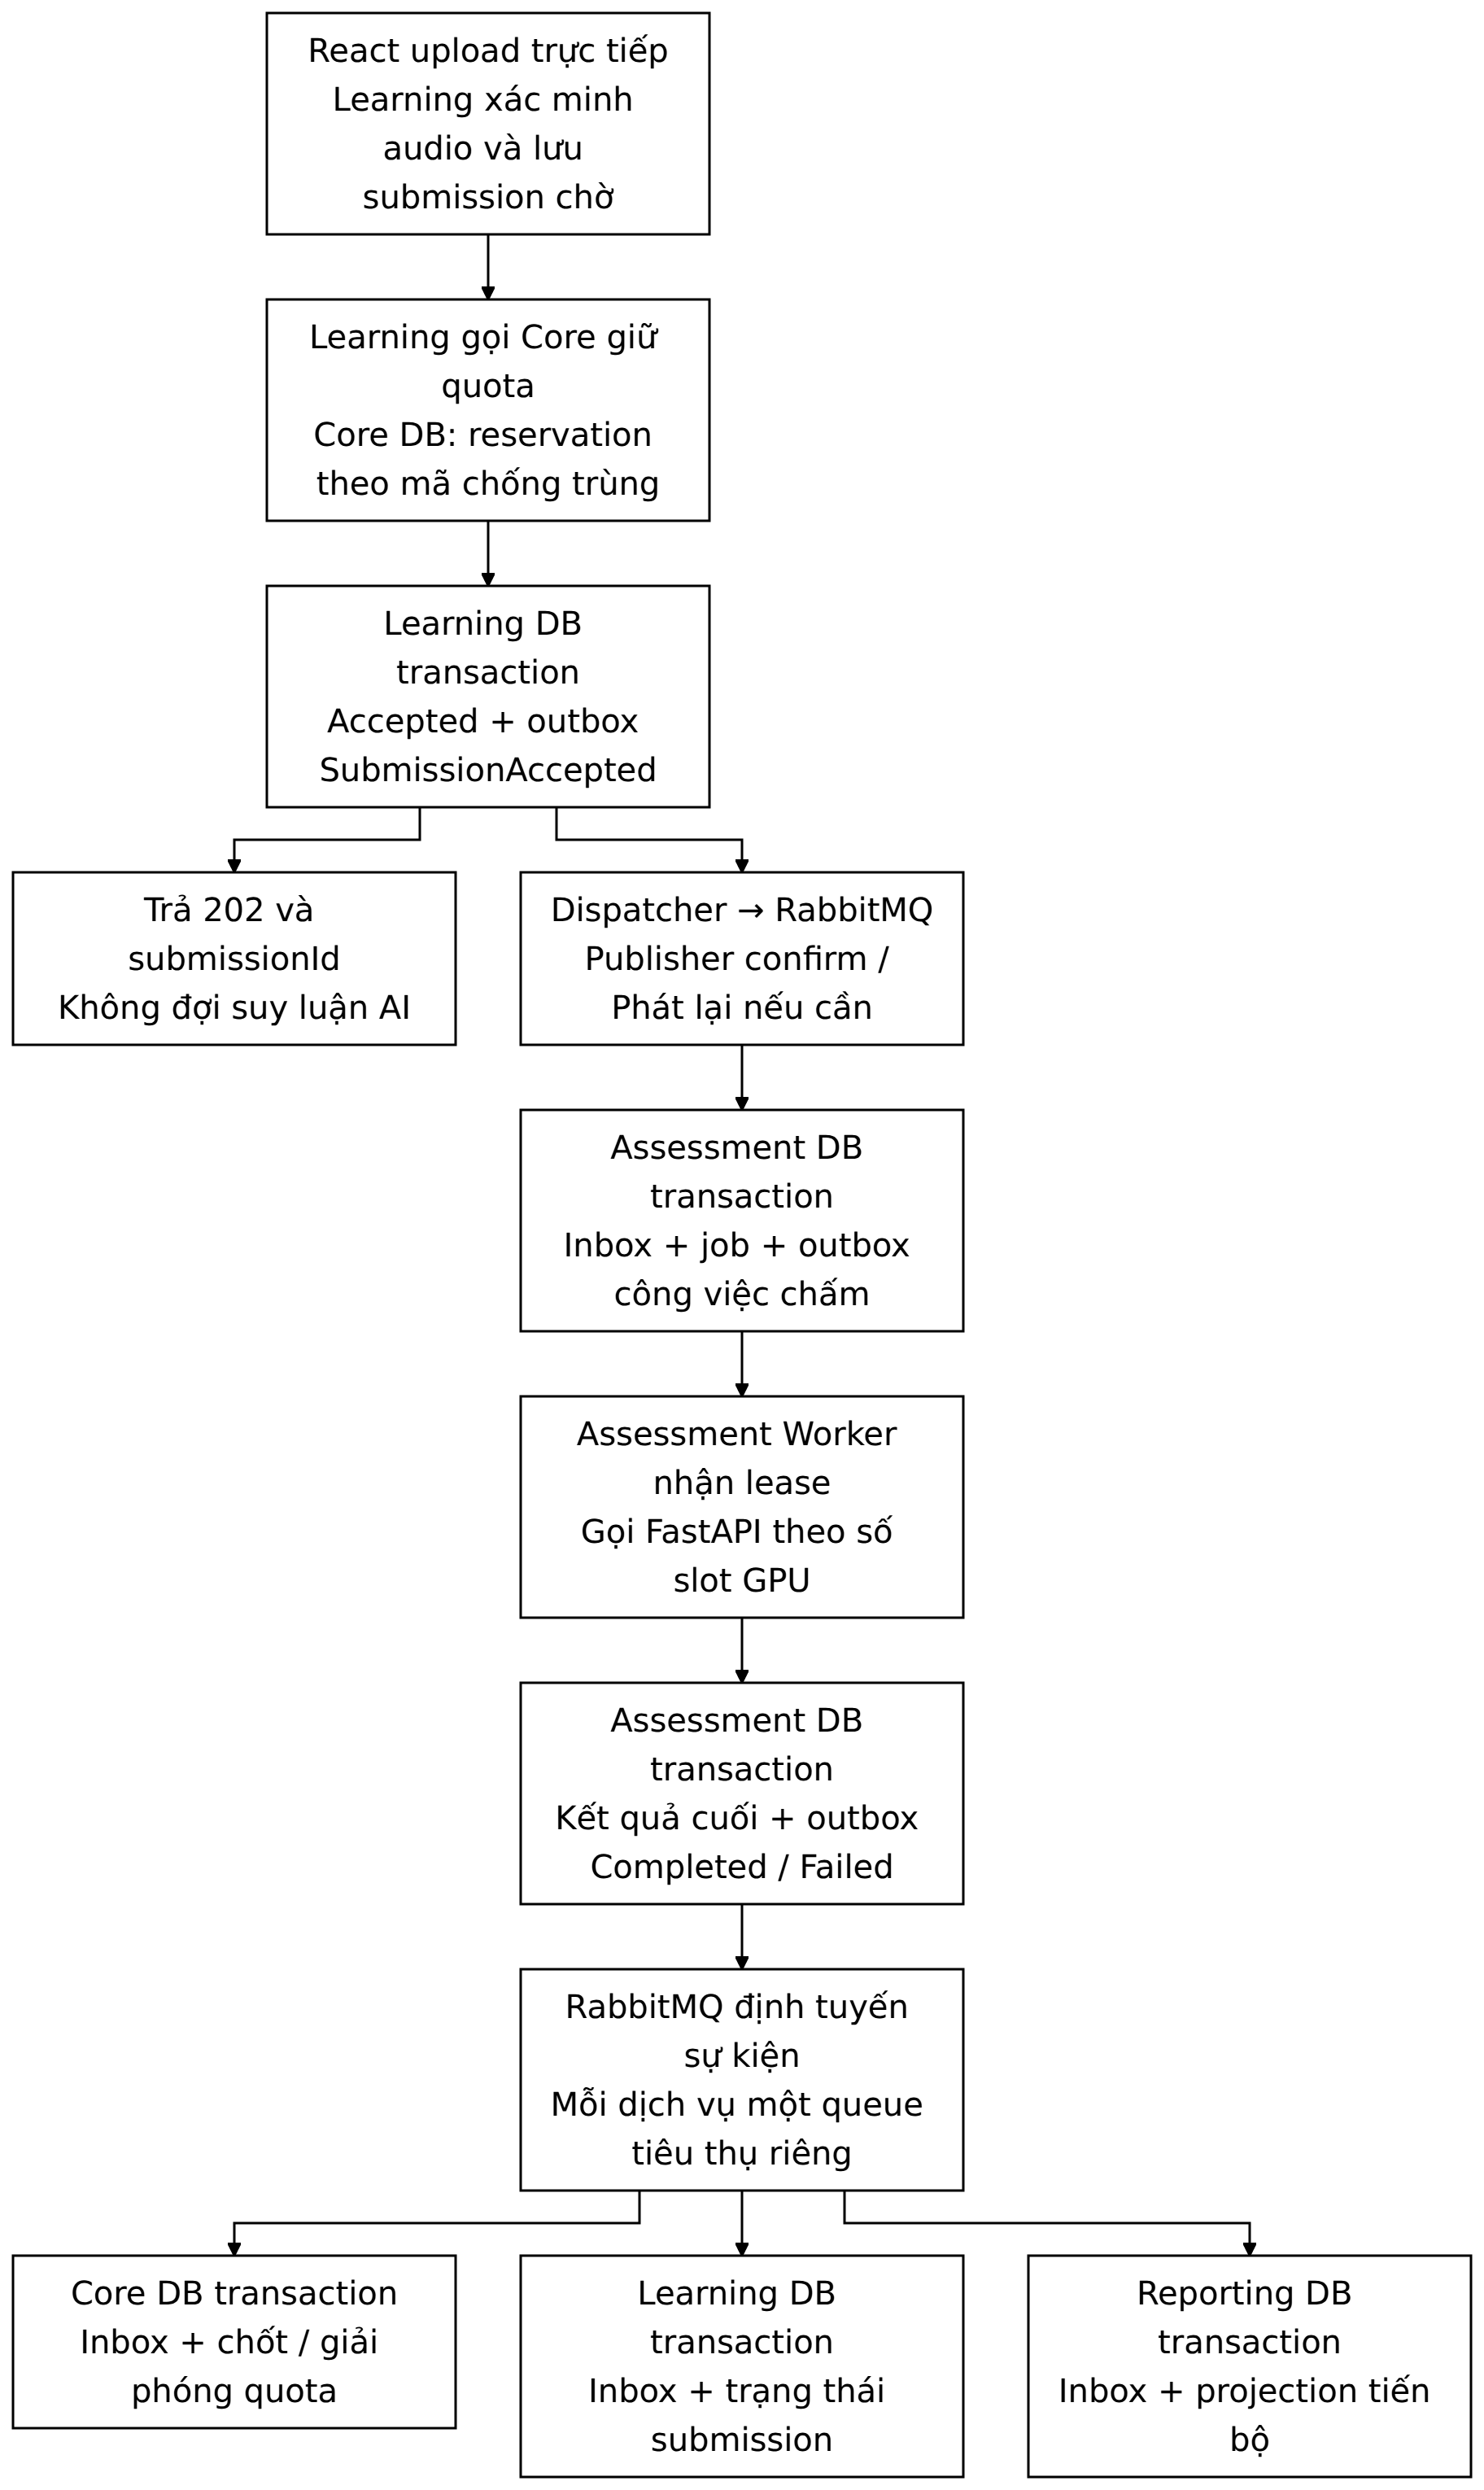
\includegraphics[width=\linewidth,height=.72\textheight,keepaspectratio]{Images/Design/speaking_flow.png}
\caption{Luồng chấm Speaking và giao dịch cục bộ giữa các dịch vụ}
\label{design:fig:speaking_flow}\end{figure}

\begingroup\emergencystretch=2em
Assessment lưu kết quả cuối cùng và sự kiện \texttt{Assessment\allowbreak{}Completed} hoặc \texttt{Assessment\allowbreak{}Failed} trong cùng transaction của Assessment DB. Core tiêu thụ sự kiện để chốt hoặc giải phóng reservation trong Core DB, chống trùng theo \texttt{event\allowbreak{}Id} và mã nghiệp vụ; Learning cập nhật trạng thái bài, Reporting cập nhật bản tổng hợp bằng các queue riêng. Trạng thái chấm xong và trạng thái đối soát quota có thể đến khác thời điểm; UI không biến độ trễ sự kiện thành yêu cầu nộp hoặc tính phí mới.
\par\endgroup

\paragraph*{Lựa chọn RabbitMQ và hợp đồng sự kiện}

RabbitMQ được dùng cho phân phối việc chấm và trao đổi sự kiện nghiệp vụ, phù hợp với nhu cầu chia công việc cho các Worker \cite{ch7_rabbitmq_workqueues}. Hai mục đích có queue riêng: một công việc chỉ cần một Worker xử lý tại một thời điểm, còn sự kiện kết quả được định tuyến vào các queue riêng của Core, Learning và Reporting để mỗi bên đều nhận được. Các consumer trong cùng một queue cạnh tranh công việc; không dùng chung queue cho ba bên với kỳ vọng mỗi bên đều nhận mọi sự kiện.

Thiết kế dùng durable queue, persistent message và publisher confirms; triển khai production chọn quorum queue có các replica trên các node độc lập phù hợp cấu hình cluster. Dispatcher chỉ đánh dấu đã phát khi nhận confirm và xử lý trường hợp message không định tuyến được. Consumer dùng manual acknowledgement sau khi transaction cục bộ hoàn tất; inbox lưu \texttt{event\allowbreak{}Id} trong cùng transaction với hiệu ứng nghiệp vụ để chống xử lý trùng \cite{ch7_rabbitmq_confirms,ch7_rabbitmq_quorum}.

\begingroup\emergencystretch=2em
Mỗi sự kiện có \texttt{event\allowbreak{}Id}, \texttt{event\allowbreak{}Type}, \texttt{schema\allowbreak{}Version}, \texttt{occurred\allowbreak{}At}, traceId, \texttt{aggregate\allowbreak{}Id} và \texttt{aggregate\allowbreak{}Version}, cùng các định danh submission, job, user và reservation cần thiết. Consumer kiểm tra phiên bản và trạng thái chuyển tiếp, xử lý sự kiện đến trễ hoặc trùng; không giả định thứ tự toàn cục giữa các queue. Retry có backoff và dead-letter queue, không requeue vô hạn. Timeout acknowledgement và lease được cấu hình phù hợp thời hạn thực thi; giám sát cả message chưa ack để tránh giữ việc trên Worker đã lỗi. Không đưa audio, secret hoặc URL riêng tư dài hạn vào sự kiện. Bản tổng hợp được tái tạo từ snapshot có mốc phiên bản qua API xuất dữ liệu có kiểm soát của Assessment, rồi áp dụng sự kiện tiếp theo bằng khóa chống trùng. RabbitMQ không được dùng làm kho lịch sử duy nhất: dữ liệu nghiệp vụ và outbox được lưu theo chính sách để đối soát hoặc xây dựng lại projection. Kafka chưa nằm trong phạm vi triển khai này.
\par\endgroup

\paragraph*{Thực thi và khả năng khôi phục}

Worker nhận thông điệp chỉ chứa định danh cần thiết như \texttt{job\allowbreak{}Id}, \texttt{source}, \texttt{trace\allowbreak{}Id} và phiên bản hợp đồng. Audio không được đặt trực tiếp trong thông điệp. Trước khi gọi AI, Worker đọc lại trạng thái job và giành quyền thực thi bằng cập nhật có điều kiện, kèm lease và số thứ tự lần thực thi.

Mỗi lần xử lý có \texttt{attempt\allowbreak{}Id} riêng. Kết quả chỉ được chấp nhận nếu attempt vẫn là chủ sở hữu hợp lệ của job. Một tác vụ theo dõi phát hiện lease hết hạn để đưa công việc về diện cần khôi phục. Cách này hạn chế việc Worker cũ trả kết quả muộn sau khi một Worker khác đã tiếp nhận công việc.

Thông điệp được xác nhận sau khi kết quả hoặc quyết định thử lại/thất bại đã được ghi bền vững. RabbitMQ và HTTP không tạo bảo đảm suy luận chỉ chạy đúng một lần. Suy luận có thể bị lặp khi xảy ra lỗi mạng; hiệu ứng nghiệp vụ được chống lặp bằng khóa công việc, ràng buộc kết quả và sổ quota.

FastAPI nhận cùng \texttt{inference\allowbreak{}Id} trong những lần gửi lại của một attempt. Có thể bổ sung cơ chế gộp yêu cầu đang chạy hoặc tra cứu kết quả theo định danh để giảm suy luận lặp. Dù có cơ chế này, Assessment DB vẫn quyết định attempt và kết quả cuối cùng nào được công nhận; Core DB quyết định các bút toán quota tương ứng.

\paragraph*{Trạng thái công việc và chính sách thử lại}

\begin{figure}[H]
\centering
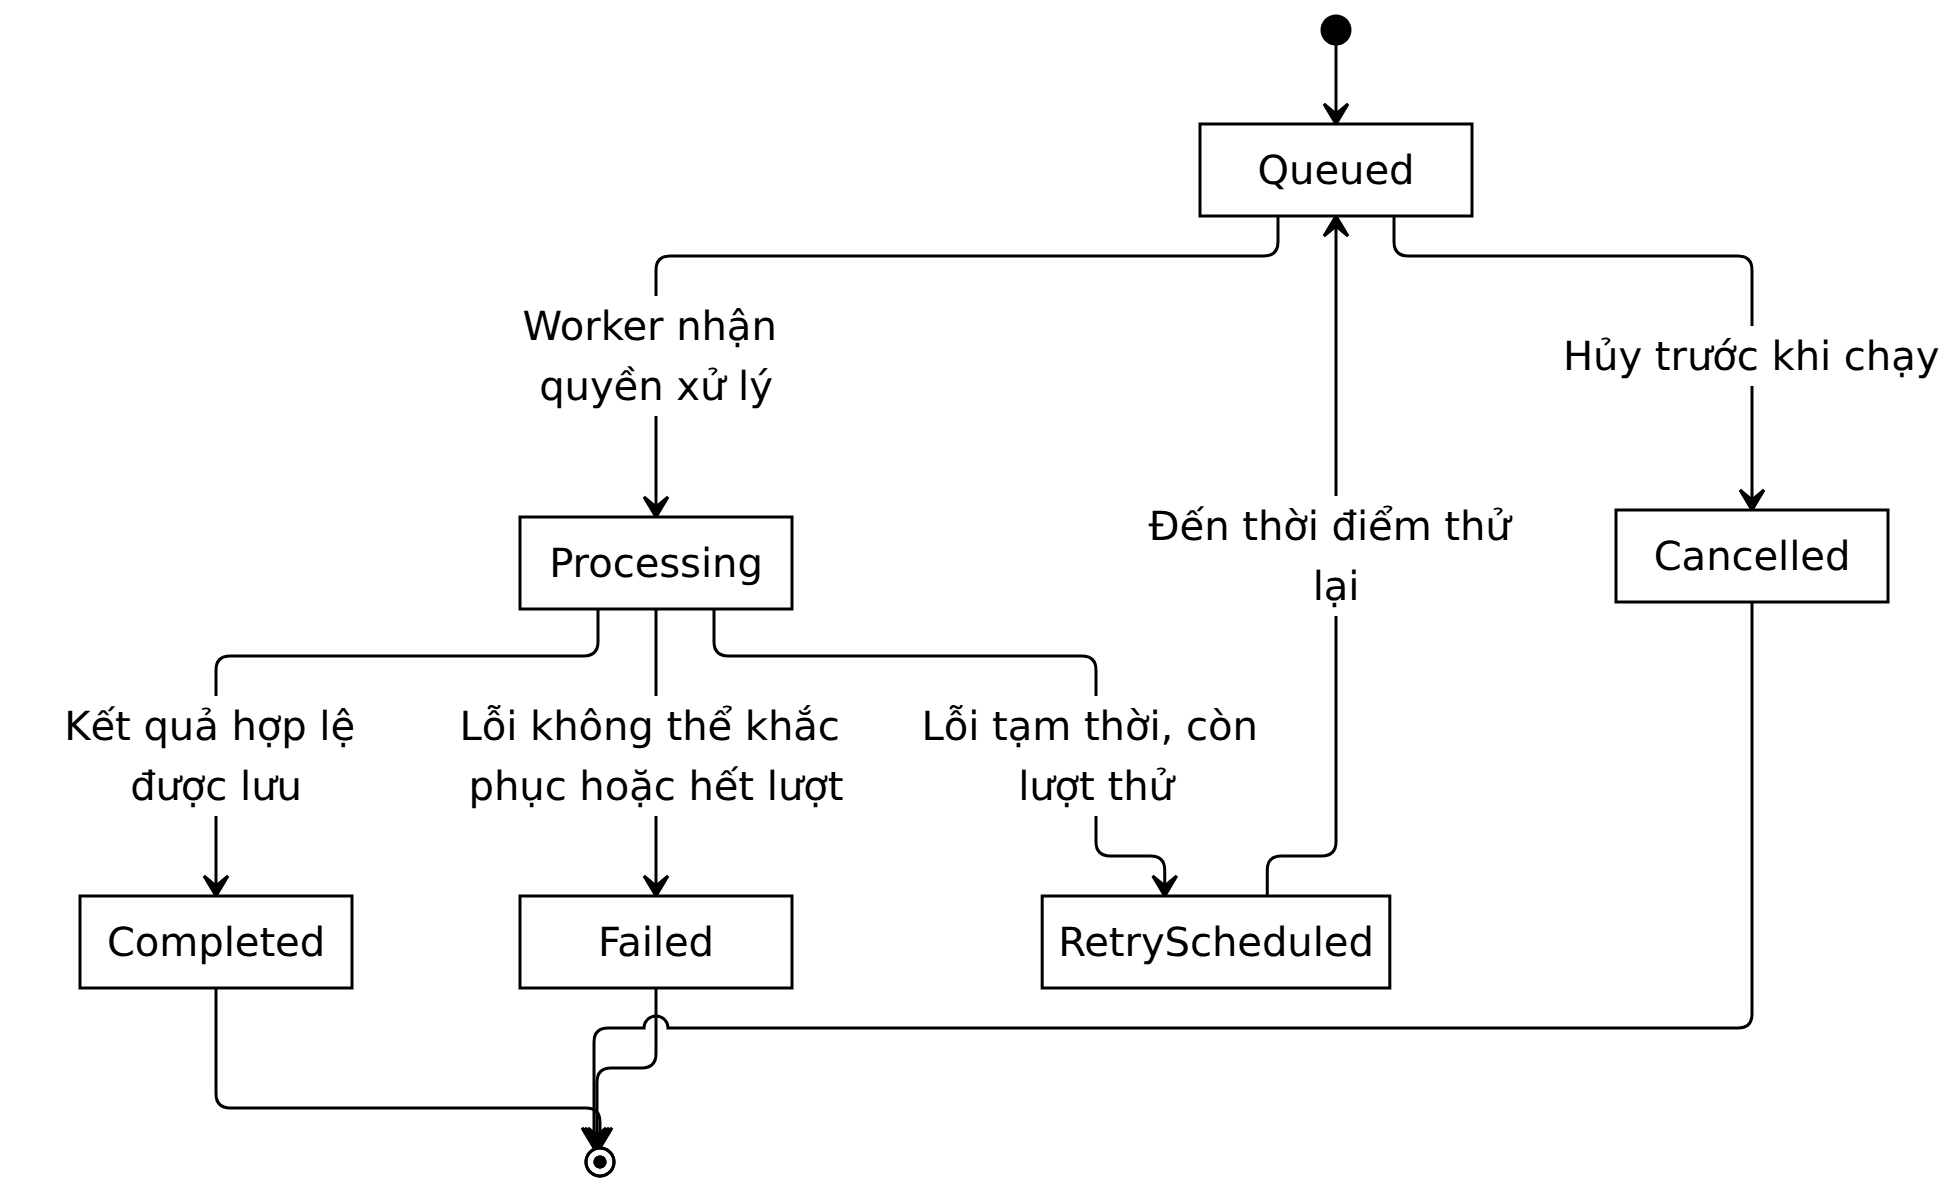
\includegraphics[width=\linewidth,height=.72\textheight,keepaspectratio]{Images/Design/assessment_states.png}
\caption{Vòng đời công việc chấm}
\label{design:fig:assessment_states}
\end{figure}

Thiết kế đề xuất quy định rõ \textbf{tối đa ba lần thực thi tự động cho một job}, gồm lần đầu và hai lần thử lại. Lỗi mạng, timeout có thể khôi phục hoặc lỗi dịch vụ tạm thời được thử lại với khoảng chờ tăng dần. Dữ liệu đầu vào không hợp lệ hoặc phiên bản mô hình không hỗ trợ không được tự động thử lại cùng dữ liệu.

Khi thất bại cuối cùng, Assessment phát sự kiện kết thúc; Core giải phóng phần quota đang giữ hoặc hoàn khoản đã trừ theo loại nghiệp vụ. Việc hoàn được ghi một lần theo mã nghiệp vụ tại Core, không nằm trong transaction lưu kết quả của Assessment. Chấm lại bài thất bại tạo yêu cầu có liên kết tới job trước và áp dụng chính sách miễn trừ quota đã đặc tả; một lần thử kỹ thuật không được biến thành một lượt luyện mới.

Đối với luyện theo Part, quota được giữ khi nhận bài và chốt sau khi chấm thành công. Đối với thi thử, Learning tạo yêu cầu bắt đầu có định danh, Core trừ một lượt thi rồi Learning xác nhận phiên được bắt đầu. Trạng thái bắt đầu dở dang được đối soát như submission; một lần gọi lại dùng cùng mã không trừ thêm lượt. Công việc chấm từng câu dùng ticket của phiên. Assessment tổng hợp trạng thái kết thúc toàn phiên theo manifest trước khi phát quyết định hoàn; không hoàn toàn bộ lượt thi cho mỗi câu bị lỗi. Kết quả phản hồi muộn từ một job đã thất bại cuối cùng không tự động chuyển thành công sau khi quota đã được hoàn.

\paragraph*{Hợp đồng tích hợp với Scoring Model}

FastAPI cung cấp endpoint nội bộ, chẳng hạn \texttt{POST /\allowbreak{}internal/\allowbreak{}v1/\allowbreak{}speaking/\allowbreak{}assessments}. Đây là hợp đồng đề xuất của thiết kế, không phải endpoint đã được xác nhận trong mã nguồn ứng dụng.

Yêu cầu suy luận có thể được chuẩn hóa như sau:

\begingroup\small
\begin{verbatim}
{
  "inferenceId": "uuid-cua-attempt",
  "jobId": "uuid-cua-cong-viec",
  "traceId": "ma-truy-vet",
  "audio": {
    "readUrl": "url-ky-tam-thoi-duoc-cap-khi-thuc-thi",
    "sha256": "checksum-audio",
    "contentType": "audio/webm"
  },
  "question": {
    "part": 2,
    "text": "Describe a skill you would like to learn.",
    "language": "en"
  },
  "modelVersion": "speaking-model-version",
  "rubricVersion": "ielts-speaking-rubric-version"
}
\end{verbatim}
\endgroup

Phản hồi cần chứa \texttt{inference\allowbreak{}Id}, phiên bản mô hình thực tế, phiên bản hợp đồng, transcript có mốc thời gian, điểm FC/LR/GRA/P, band tổng, lỗi và nhận xét. Kết quả phải phân biệt được trường hợp đầy đủ, trường hợp thiếu dữ liệu và trường hợp không đủ điều kiện chấm.

Backend kiểm tra kiểu dữ liệu, miền điểm, mốc thời gian, mã định danh và phiên bản trước khi lưu. Điểm theo thang 0–9, bước 0,5 được xử lý theo hợp đồng đã thống nhất với mô hình. Dữ liệu thiếu tiêu chí bắt buộc không được chuyển thành báo cáo đủ bốn tiêu chí bằng cách điền điểm mặc định.

Scoring Model là thành phần chịu trách nhiệm đánh giá bài nói theo giả định của đề tài. LLM bên ngoài có thể hỗ trợ câu trả lời mẫu hoặc giải thích, nhưng không được tự động thay thế kết quả phát âm và band Speaking của mô hình bằng đánh giá chỉ dựa trên transcript.

\paragraph*{Tiền xử lý và vận hành FastAPI}

AI Runtime gồm các bước kiểm tra tệp, giải mã audio, chuẩn hóa sample rate và số kênh, kiểm tra chất lượng, suy luận, hậu xử lý và kiểm định cấu trúc kết quả. Bản audio gốc được giữ theo chính sách lưu trữ; dữ liệu chuẩn hóa phục vụ suy luận có vòng đời riêng.

Tác vụ GPU nặng không được đặt vào cơ chế \texttt{Background\allowbreak{}Tasks} trong tiến trình HTTP với kỳ vọng có hàng đợi bền vững. FastAPI cũng khuyến nghị sử dụng cơ chế xử lý riêng cho công việc nặng cần chạy qua nhiều tiến trình hoặc máy chủ \cite{ch7_fastapi_tasks}. Trong thiết kế này, .NET Worker và RabbitMQ chịu trách nhiệm điều phối bền vững; FastAPI cung cấp năng lực suy luận có giới hạn đồng thời.

Mô hình được nạp khi tiến trình AI khởi động. Số tiến trình và số yêu cầu chạy đồng thời phải phù hợp bộ nhớ GPU; không tăng số HTTP worker một cách độc lập với số bản sao trọng số. Các bước tính toán đồng bộ được thực thi trong bộ thực thi phù hợp để không chặn event loop của FastAPI. Nếu GPU hết năng lực nhận thêm việc, AI Runtime trả trạng thái quá tải để Worker điều chỉnh nhịp tiếp nhận.

\paragraph*{Thi thử và báo cáo toàn phiên}

Hệ thống tạo trước hoặc cache audio câu hỏi để giảm độ trễ giữa các câu. Trong lúc học viên nói, frontend gửi các đoạn audio theo thứ tự; backend theo dõi phần đã nhận và phần còn thiếu. Kết thúc phiên, hệ thống chỉ tạo các công việc chấm cần thiết sau khi các audio liên quan được xác minh hoàn tất.

Báo cáo thi thử liên kết kết quả theo câu, Part và phiên bản mô hình. Quy tắc tổng hợp phải thuộc hợp đồng đánh giá đã được kiểm chứng của Scoring Model. Backend không tự lấy trung bình tất cả câu để suy ra band toàn bài nếu hợp đồng mô hình chưa quy định. Bài kết thúc sớm được phân biệt với bài đủ phiên và hiển thị kết quả theo phạm vi dữ liệu thực có.

\subsubsection{Sequence diagram các chức năng Wispace}

Các sơ đồ mô tả trao đổi giữa tác nhân, React và dịch vụ sở hữu nghiệp vụ. API Gateway định tuyến và kiểm soát truy cập biên, được lược khỏi các sơ đồ để ưu tiên tương tác dịch vụ. Core, Learning, Assessment và Reporting kiểm tra quyền ở phía mình; ký hiệu DB gắn với từng dịch vụ không biểu diễn database dùng chung. Mũi tên liền biểu diễn lời gọi, mũi tên đứt biểu diễn phản hồi; các khung alt, opt, loop và par biểu diễn nhánh, bước tùy chọn, lặp và xử lý song song. Thông điệp trong luồng nền được tách khỏi phản hồi HTTP để thể hiện đúng thời điểm nhận bài và trả kết quả.

\clearpage
\paragraph*{UC01. Đăng ký tài khoản}

\begin{figure}[H]
\centering
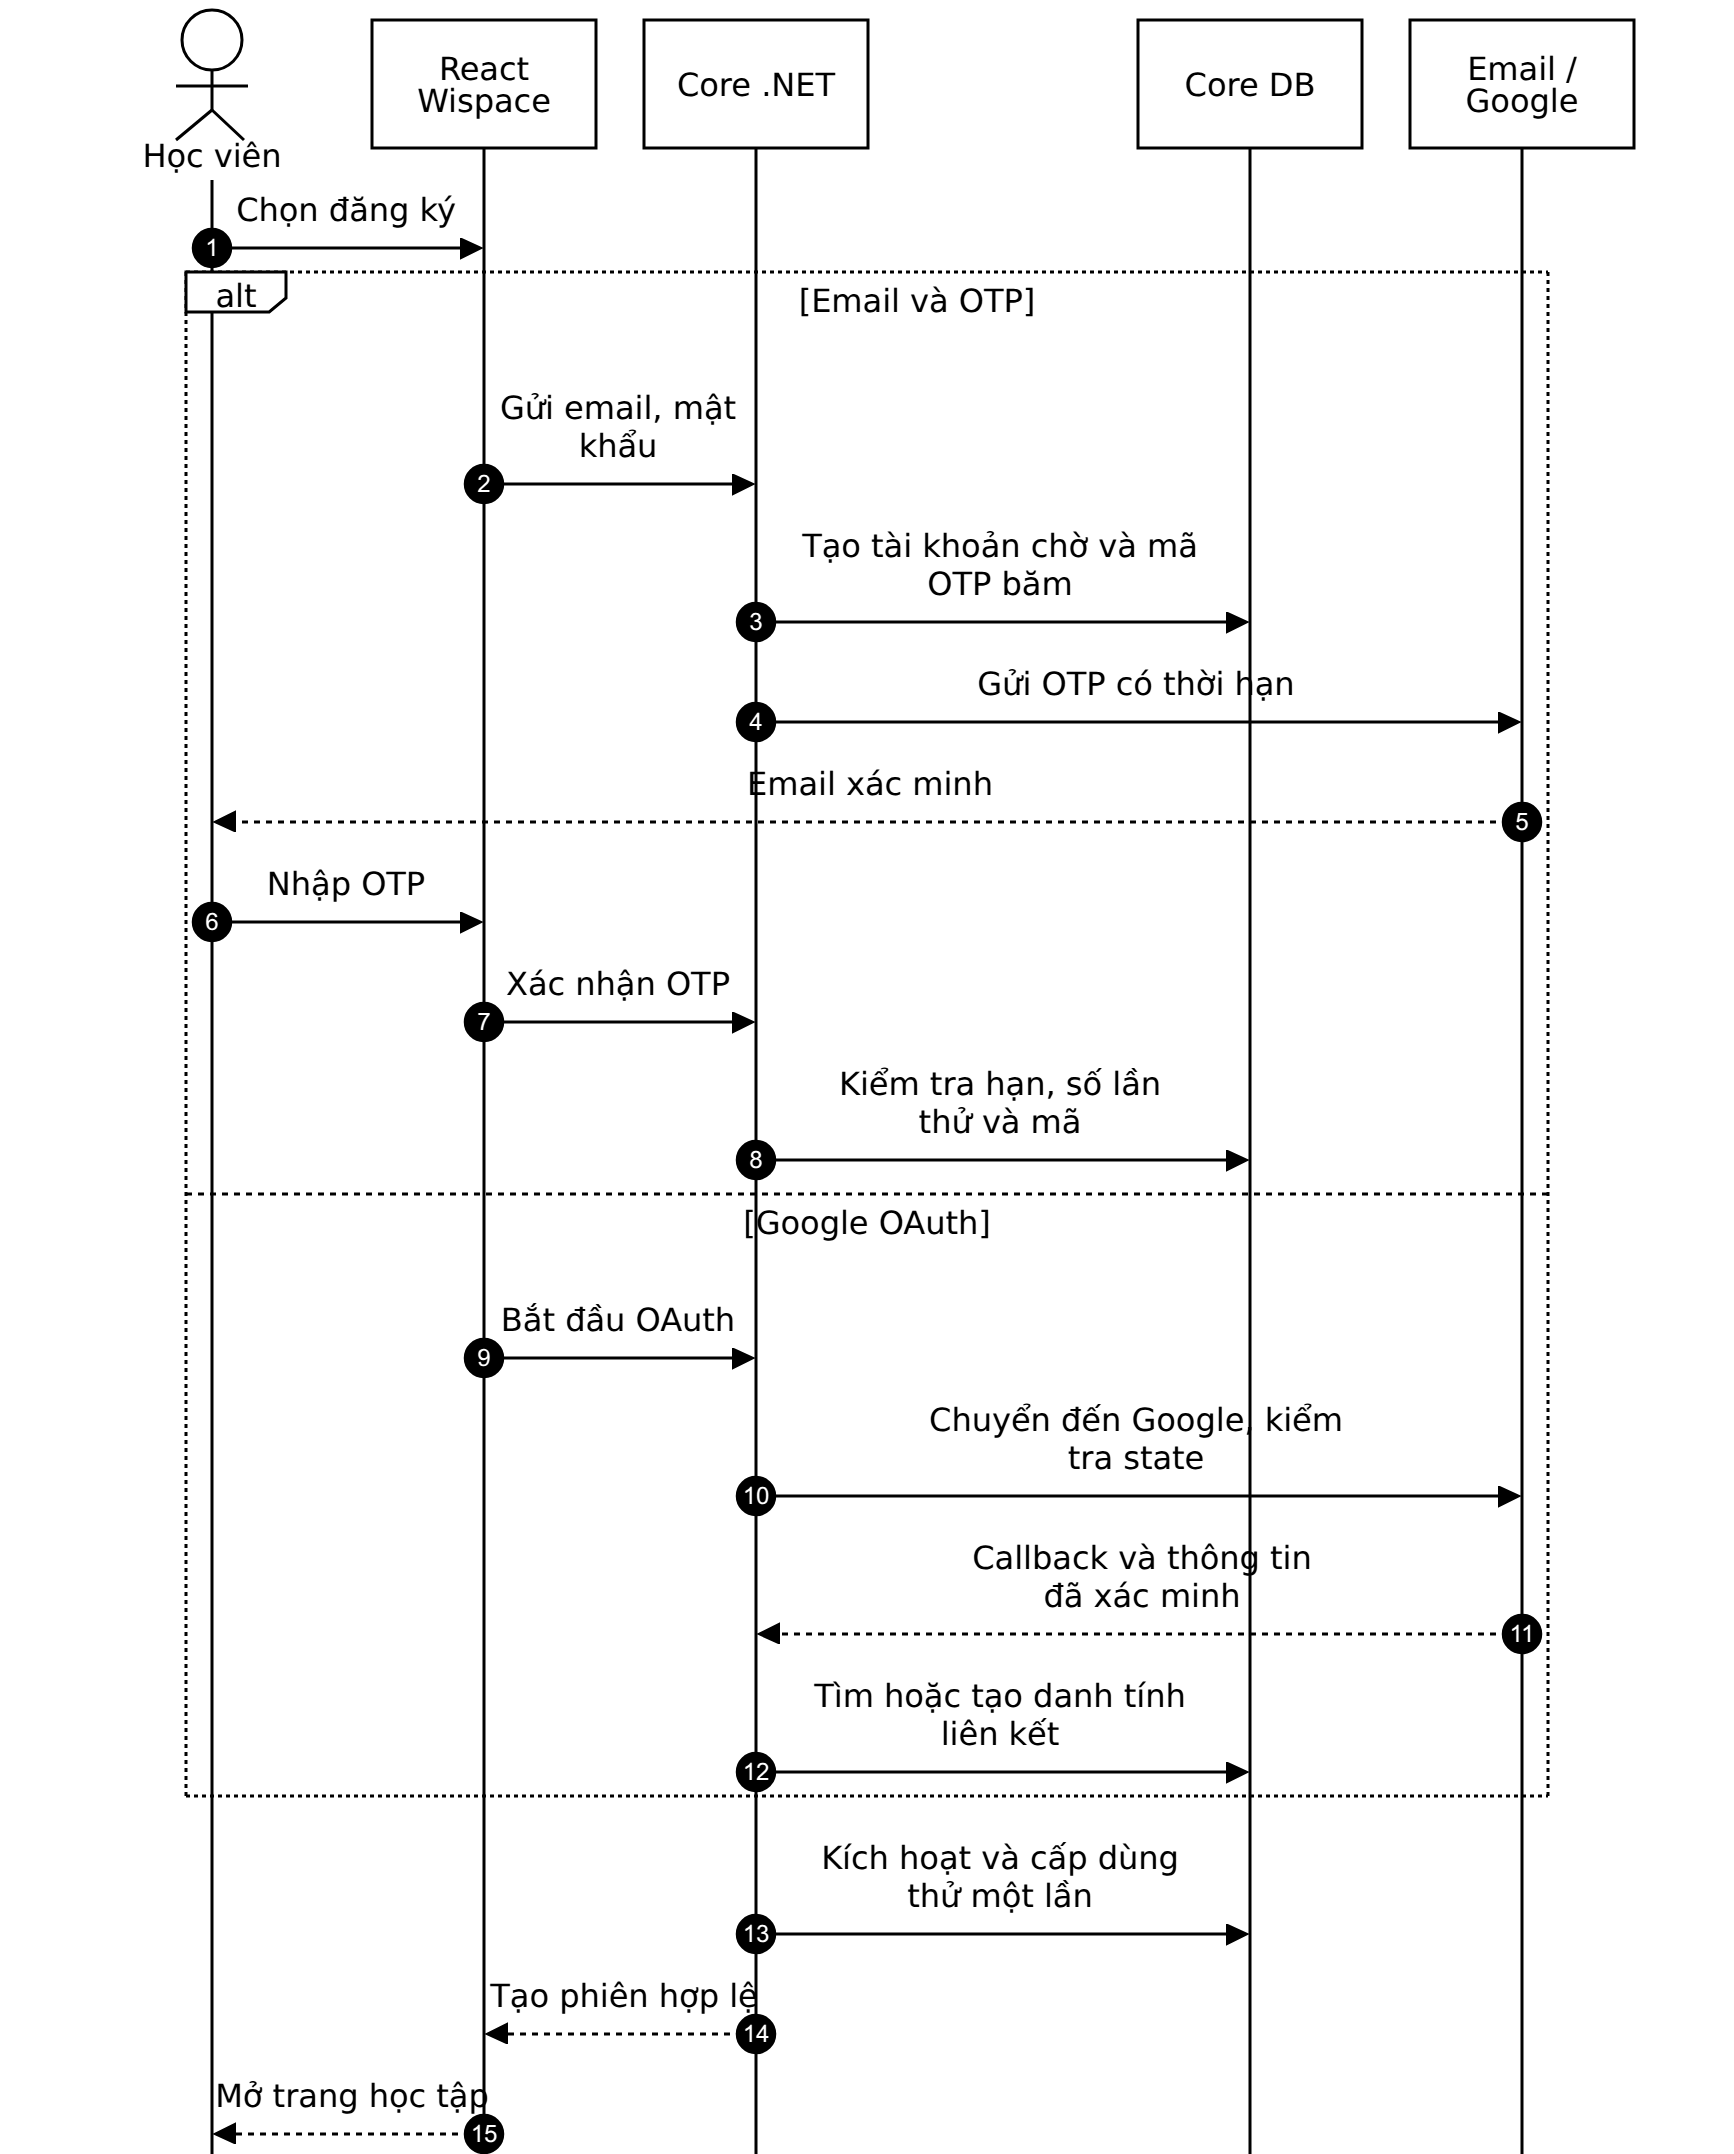
\includegraphics[width=\linewidth,height=.77\textheight,keepaspectratio]{Images/Sequence/Wispace/sequence_uc01_register.png}
\caption{Sequence diagram Wispace UC01 — Đăng ký tài khoản}
\label{sequence:wispace:sequence_uc01_register}
\end{figure}

Hai phương thức đăng ký hội tụ ở bước kích hoạt; cấp quyền lợi dùng thử và tạo tài khoản phải chống lặp.

\clearpage
\paragraph*{UC02. Đăng nhập và khôi phục mật khẩu}

\begin{figure}[H]
\centering
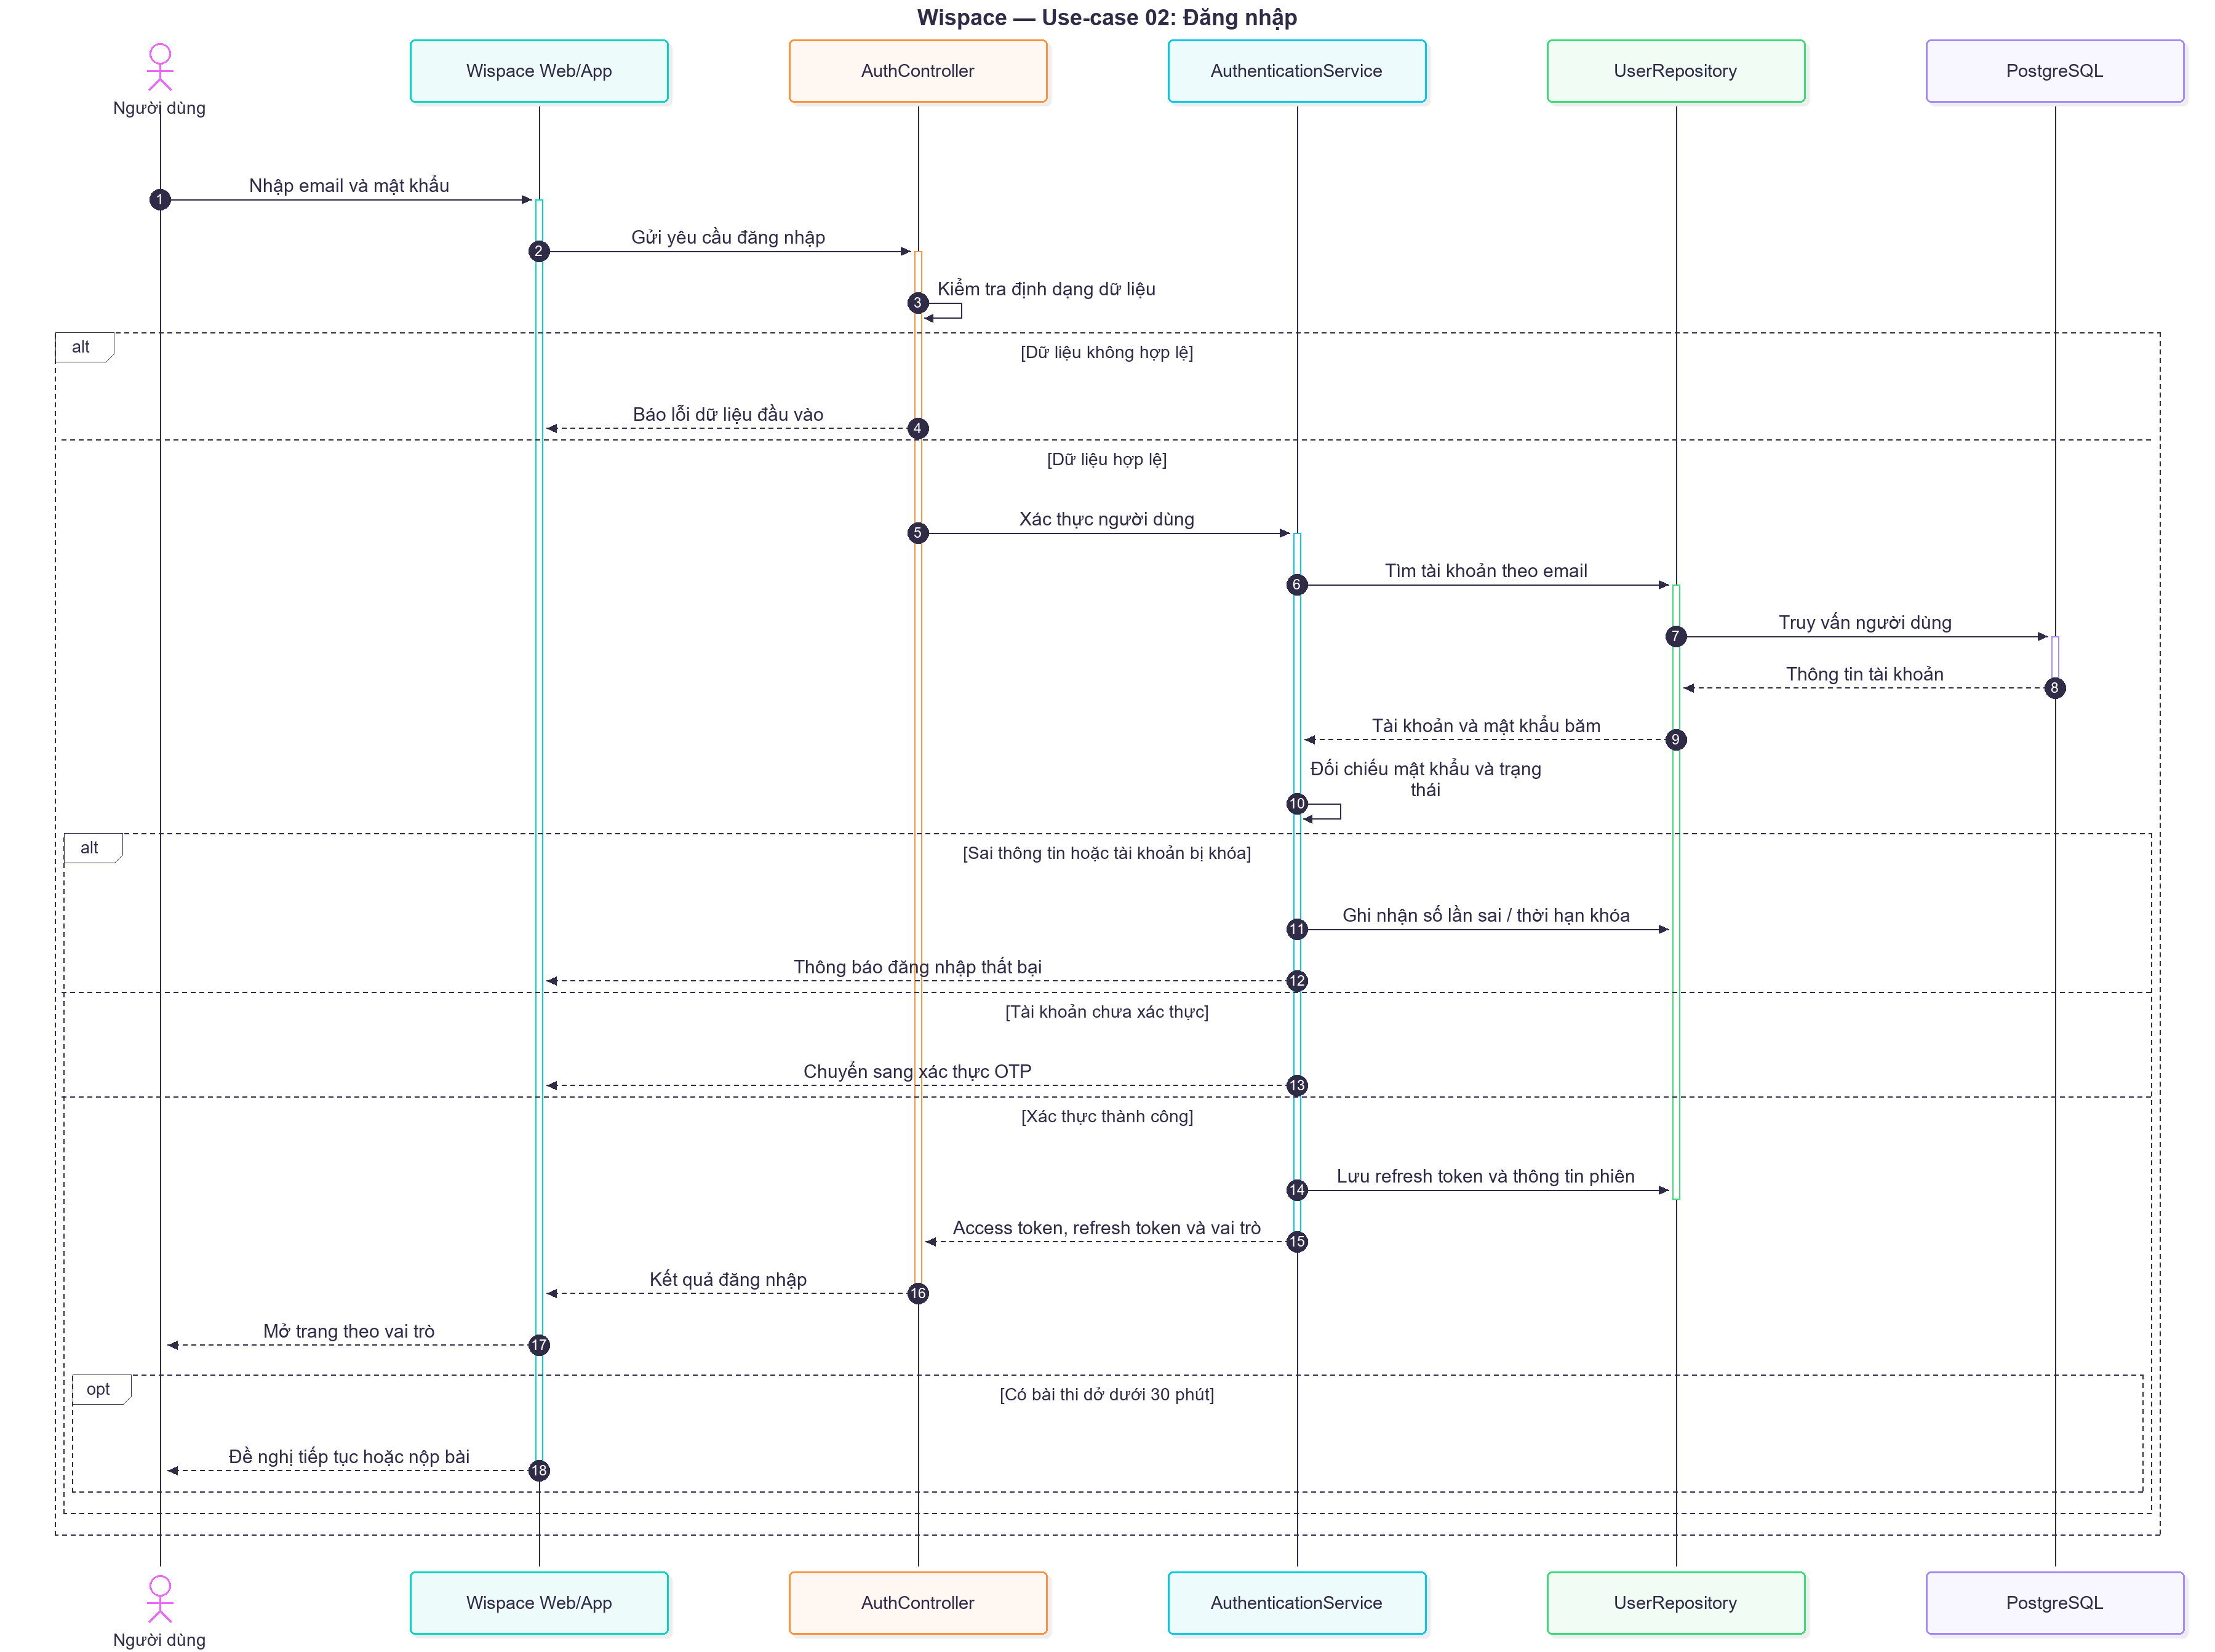
\includegraphics[width=\linewidth,height=.77\textheight,keepaspectratio]{Images/Sequence/Wispace/sequence_uc02_login.png}
\caption{Sequence diagram Wispace UC02 — Đăng nhập và khôi phục mật khẩu}
\label{sequence:wispace:sequence_uc02_login}
\end{figure}

Máy chủ kiểm tra danh tính và trạng thái trước khi cấp phiên; đặt lại mật khẩu thu hồi các phiên cũ.

\clearpage
\paragraph*{UC03. Đăng xuất}

\begin{figure}[H]
\centering
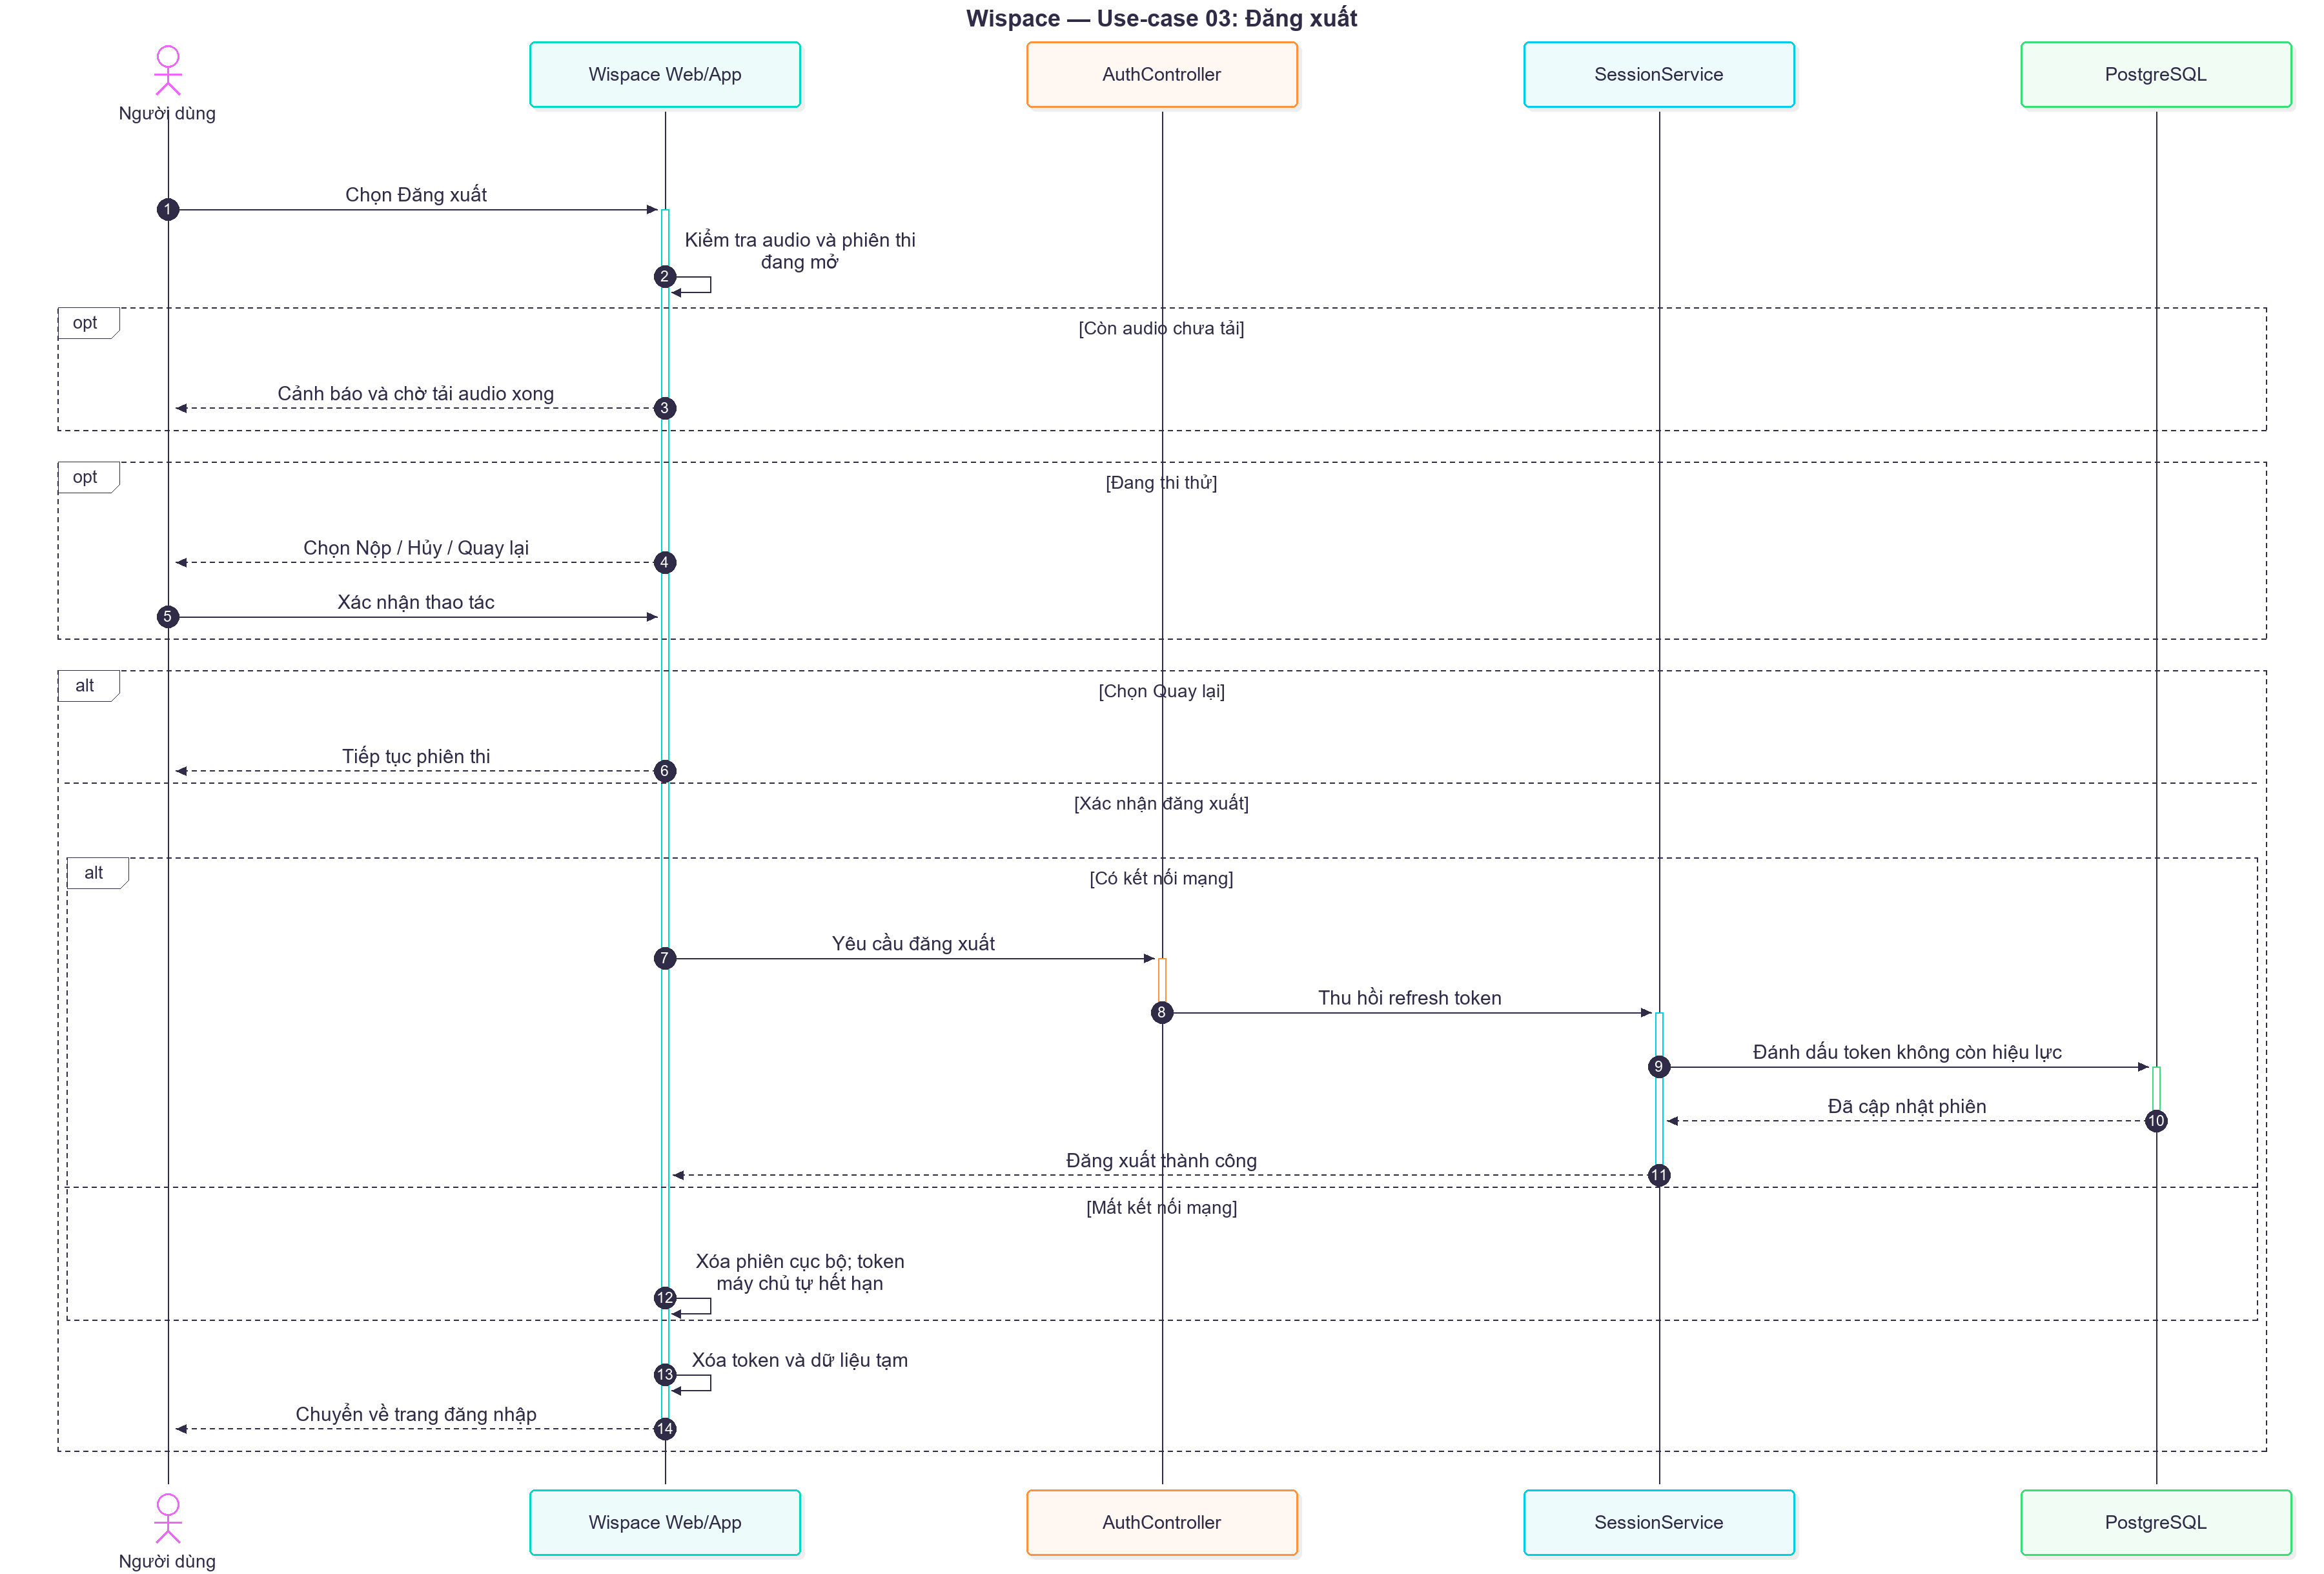
\includegraphics[width=\linewidth,height=.77\textheight,keepaspectratio]{Images/Sequence/Wispace/sequence_uc03_logout.png}
\caption{Sequence diagram Wispace UC03 — Đăng xuất}
\label{sequence:wispace:sequence_uc03_logout}
\end{figure}

Learning lưu bài trong database của mình; Core thu hồi phiên đăng nhập, không ghi trực tiếp dữ liệu phiên thi.

\clearpage
\paragraph*{UC04. Quản lý hồ sơ}

\begin{figure}[H]
\centering
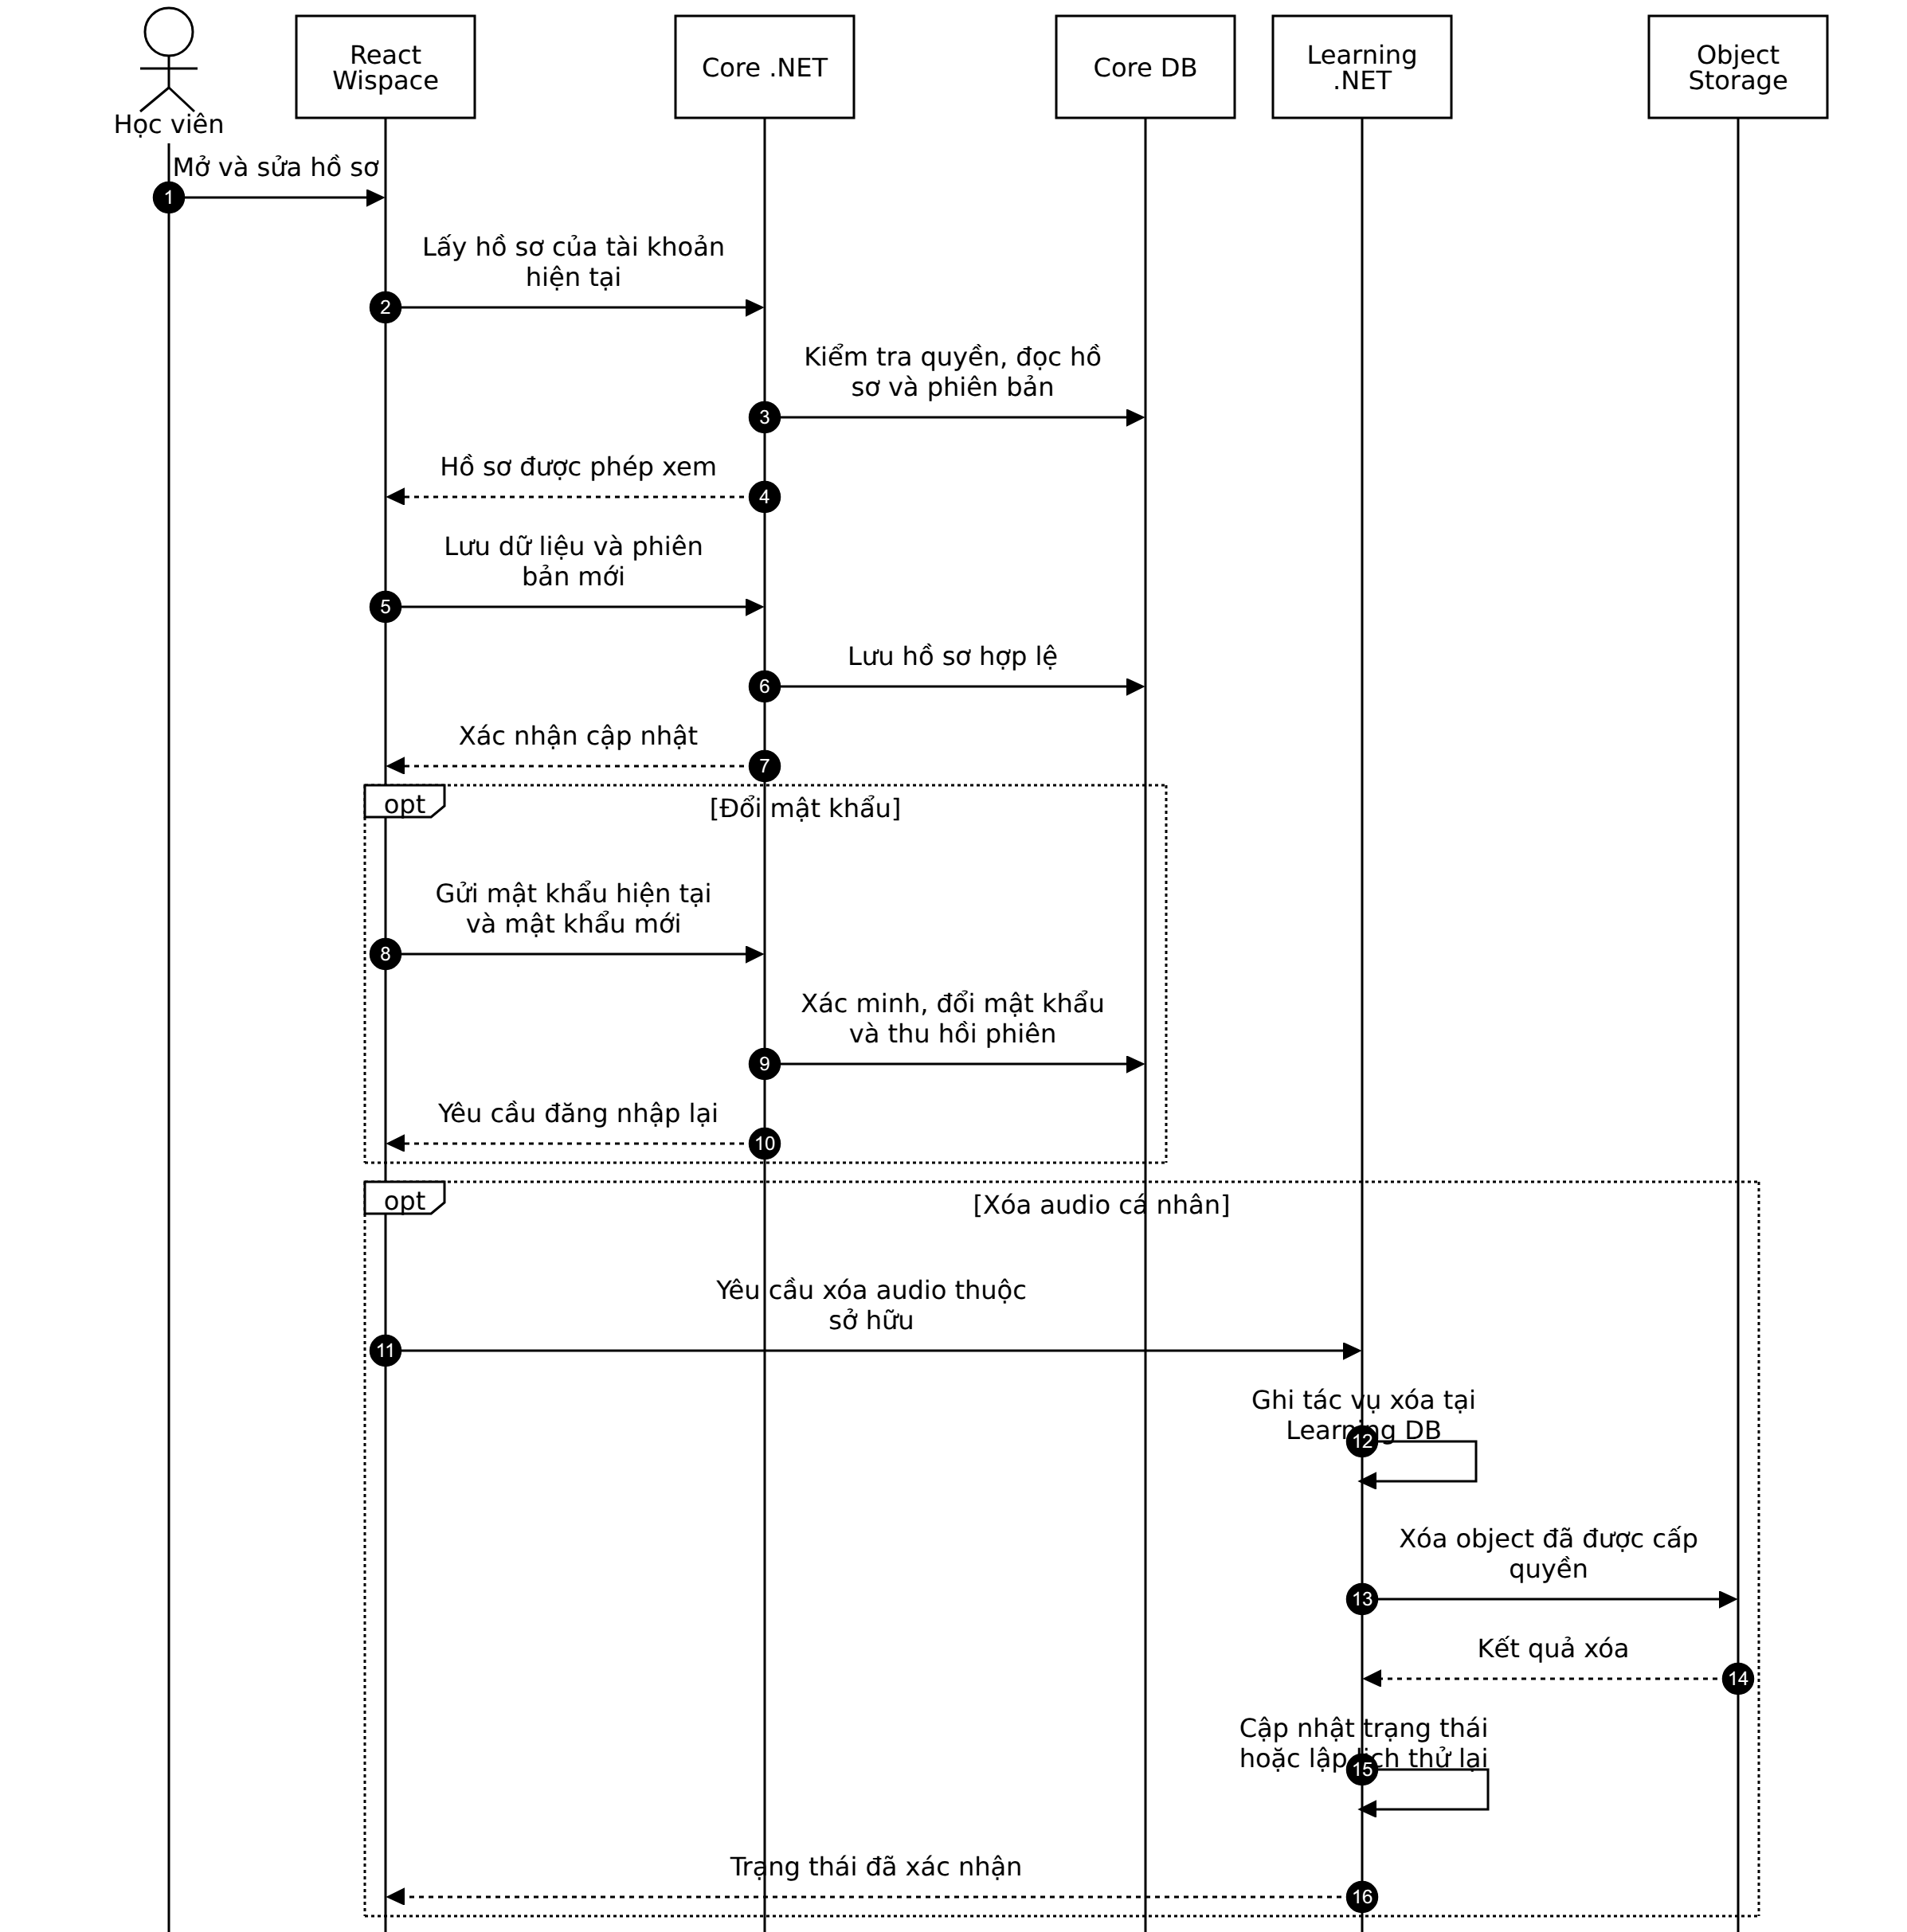
\includegraphics[width=\linewidth,height=.77\textheight,keepaspectratio]{Images/Sequence/Wispace/sequence_uc04_profile.png}
\caption{Sequence diagram Wispace UC04 — Quản lý hồ sơ}
\label{sequence:wispace:sequence_uc04_profile}
\end{figure}

Core quản lý hồ sơ; Learning quản lý quyền audio và trạng thái xóa, không có truy cập chéo database.

\clearpage
\paragraph*{UC05. Quản trị người dùng}

\begin{figure}[H]
\centering
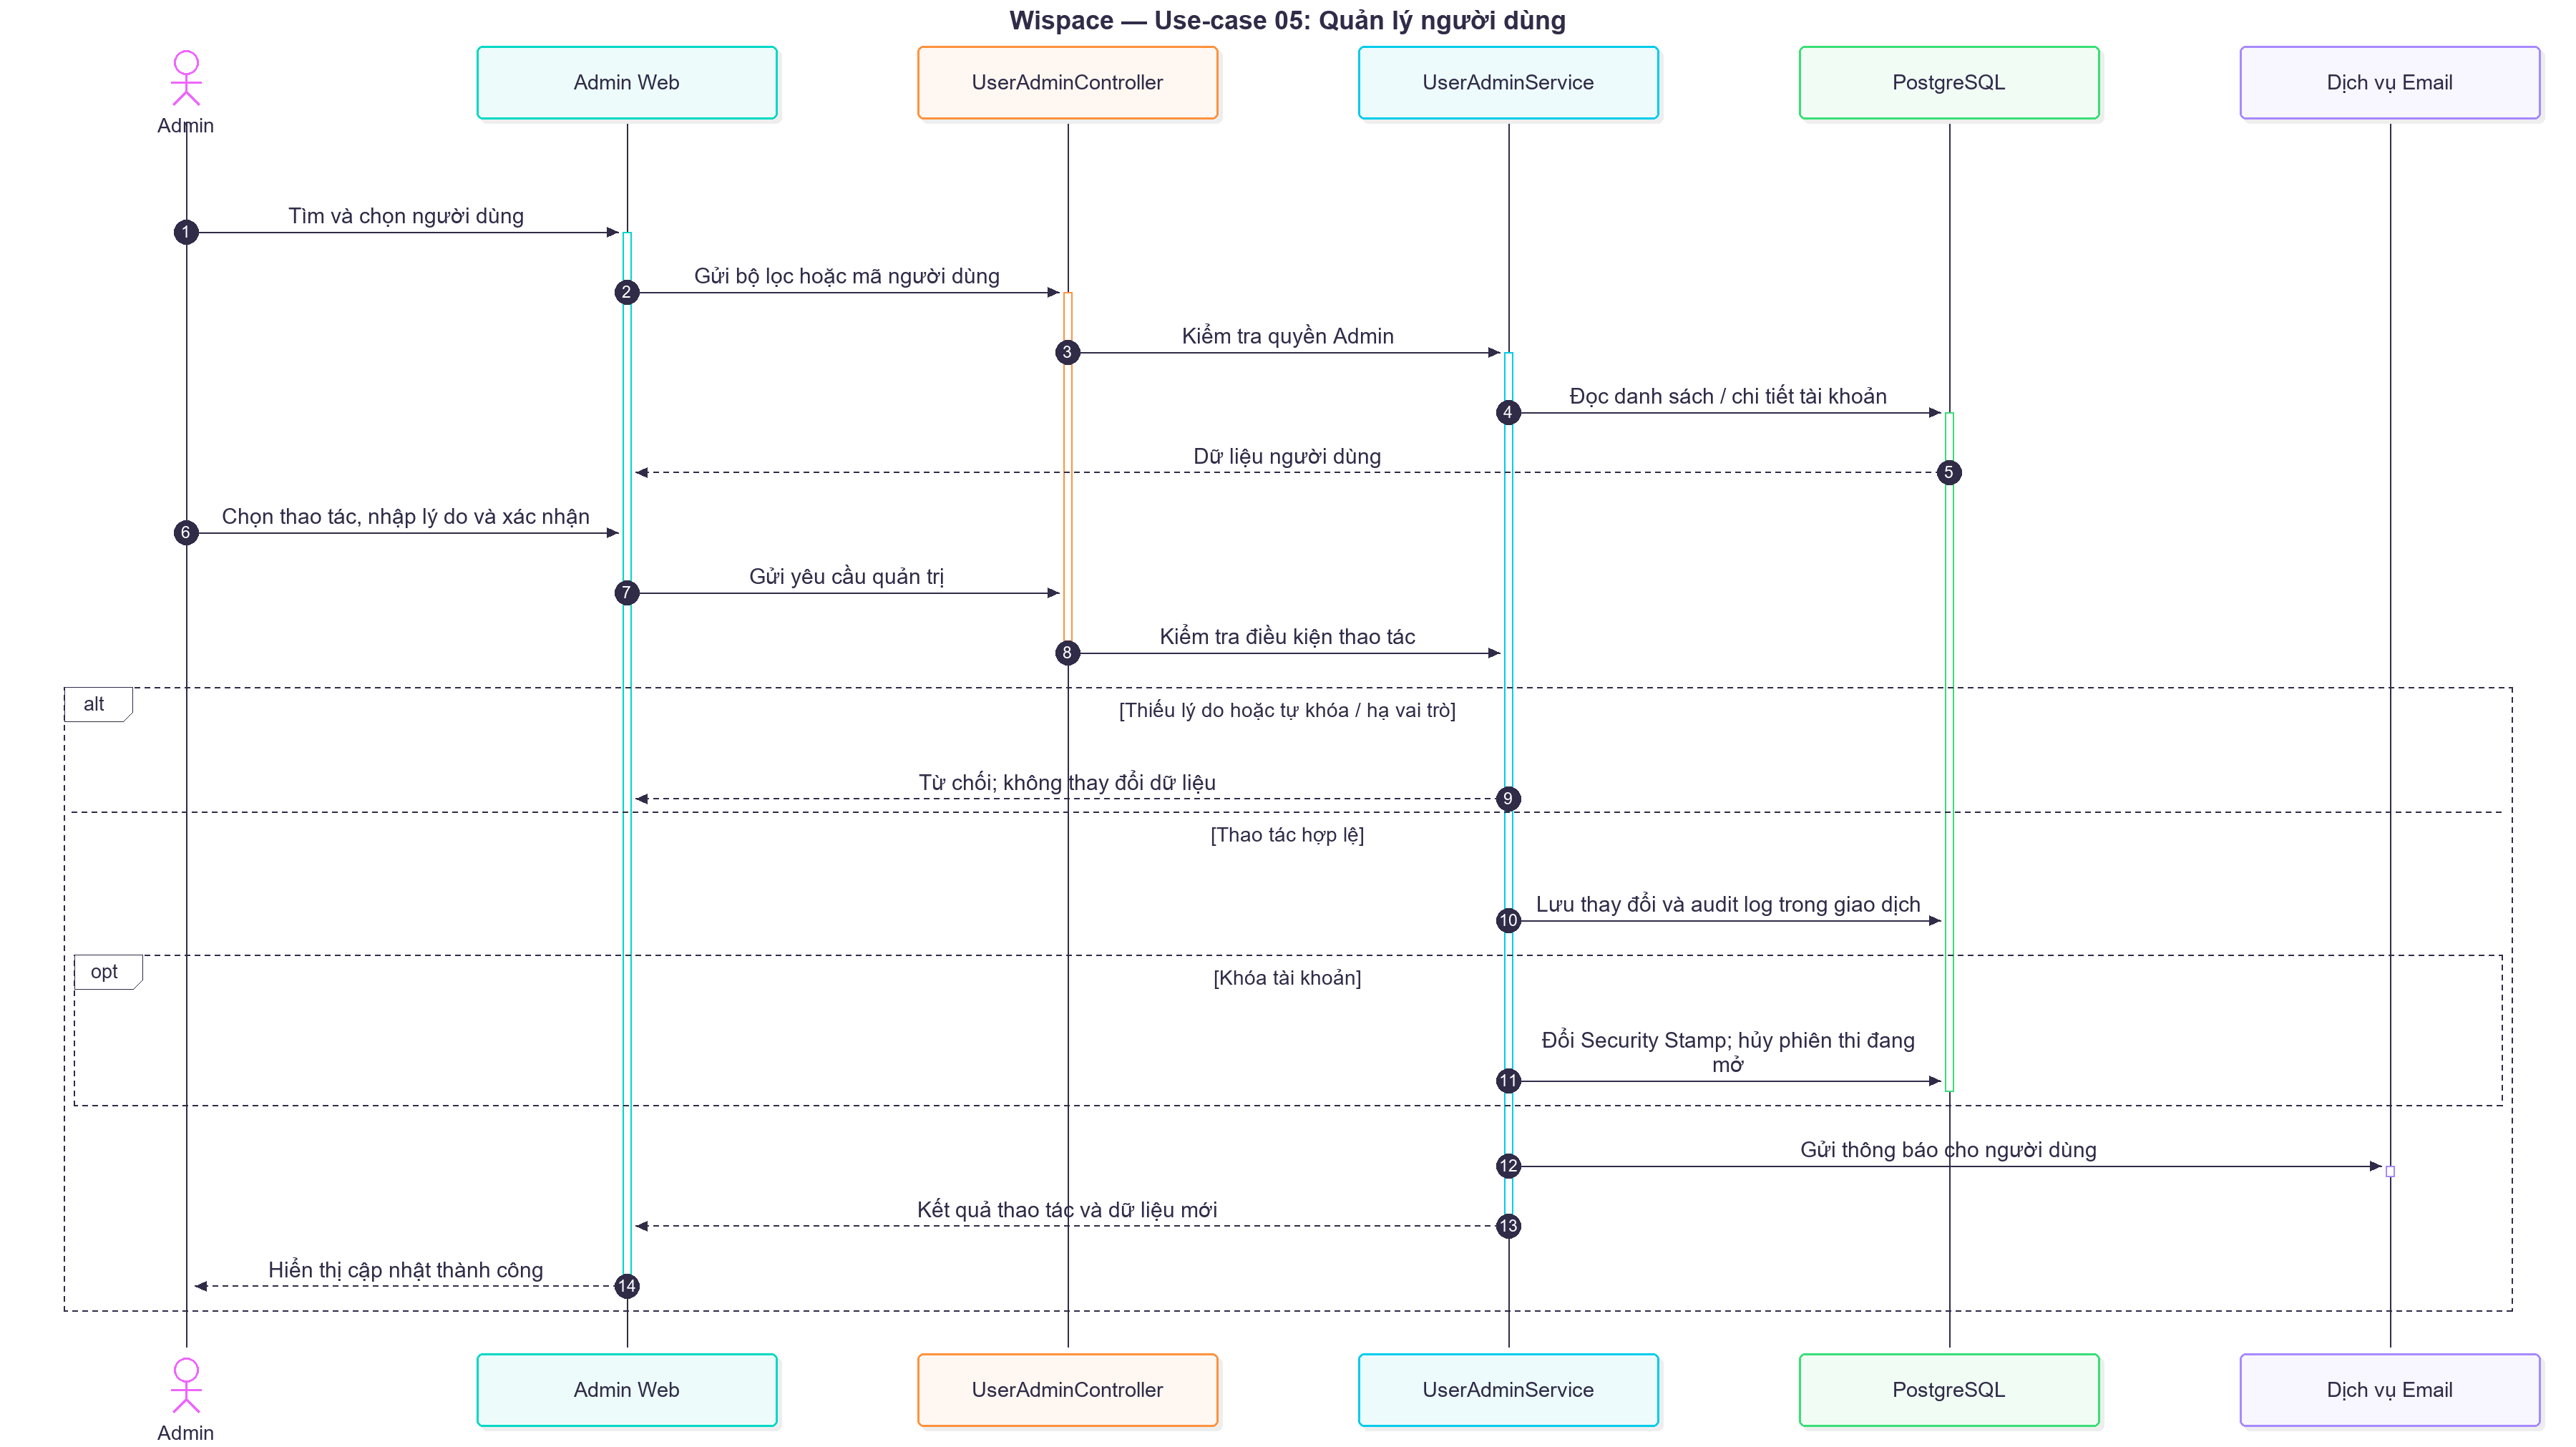
\includegraphics[width=\linewidth,height=.77\textheight,keepaspectratio]{Images/Sequence/Wispace/sequence_uc05_user_management.png}
\caption{Sequence diagram Wispace UC05 — Quản trị người dùng}
\label{sequence:wispace:sequence_uc05_user_management}
\end{figure}

Kiểm tra quyền và quy tắc tài khoản trước giao dịch; thay đổi nhạy cảm gắn với kiểm toán và thu hồi phiên.

\clearpage
\paragraph*{UC06. Xem và tìm kiếm đề}

\begin{figure}[H]
\centering
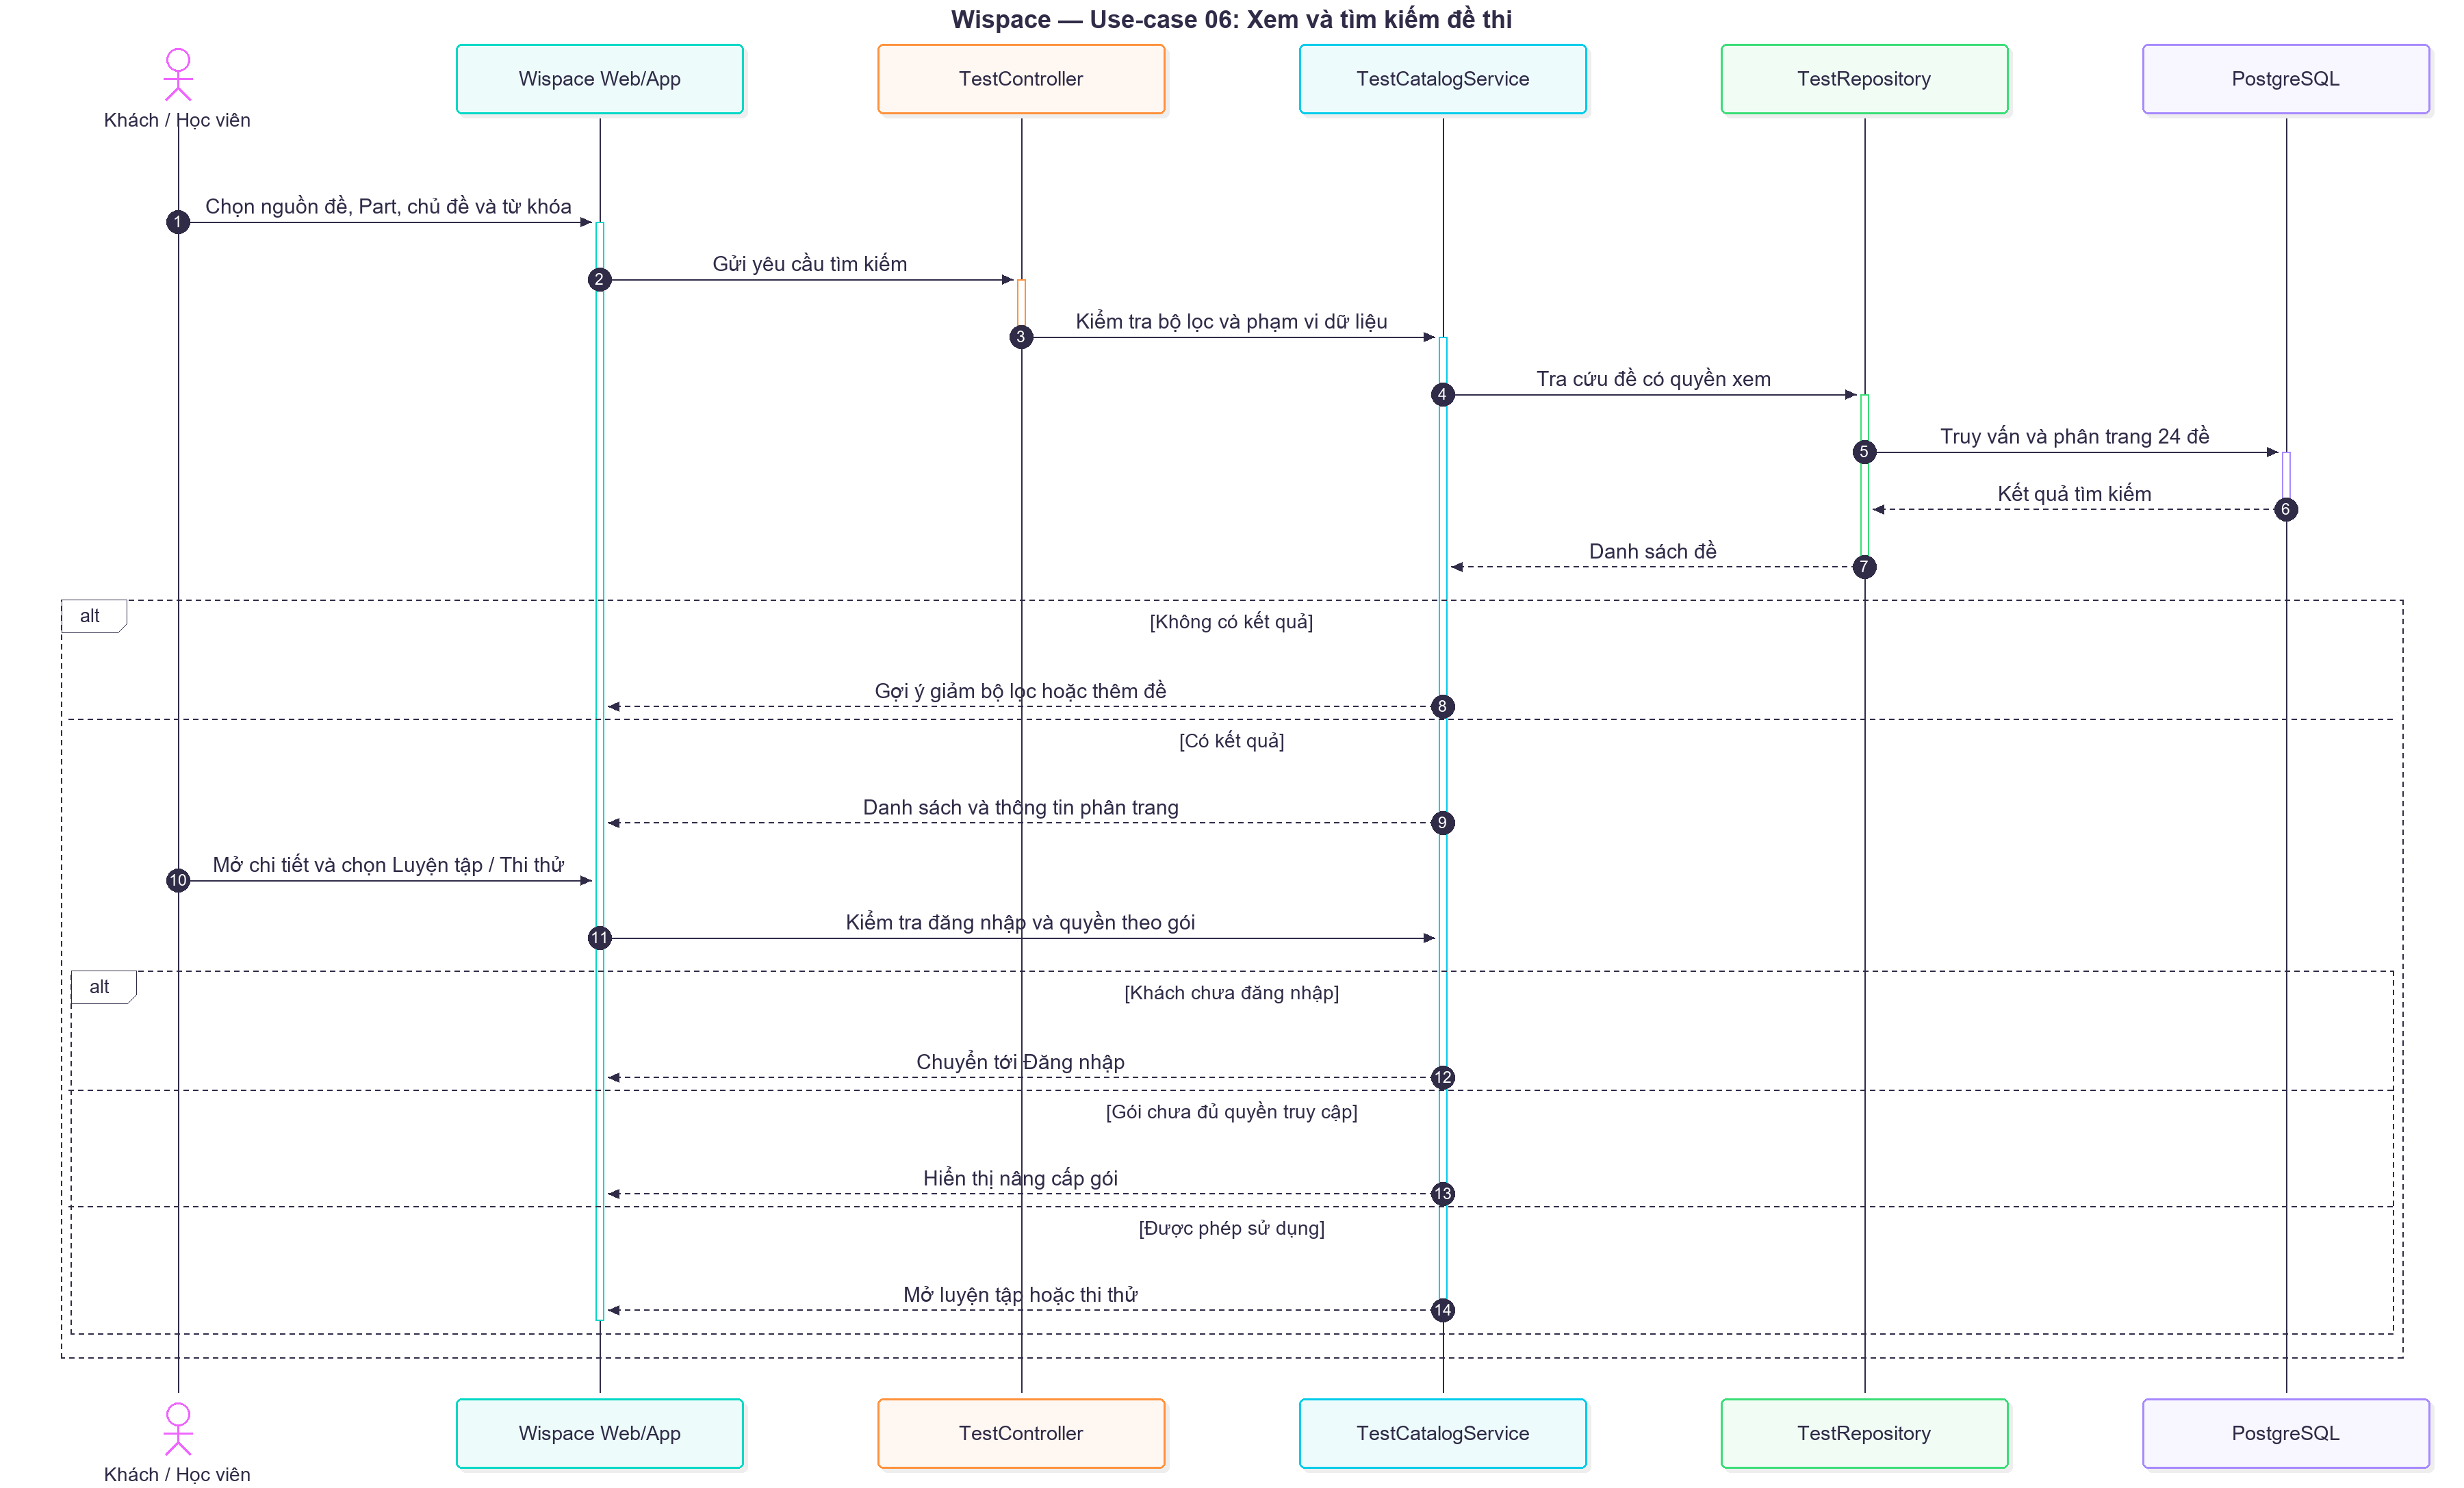
\includegraphics[width=\linewidth,height=.77\textheight,keepaspectratio]{Images/Sequence/Wispace/sequence_uc06_browse_tests.png}
\caption{Sequence diagram Wispace UC06 — Xem và tìm kiếm đề}
\label{sequence:wispace:sequence_uc06_browse_tests}
\end{figure}

Bộ lọc quyền được áp dụng trong truy vấn và kiểm tra lại ở trang chi tiết; quyền xem không đồng nghĩa quyền thi.

\clearpage
\paragraph*{UC07. Thêm đề luyện tập}

\begin{figure}[H]
\centering
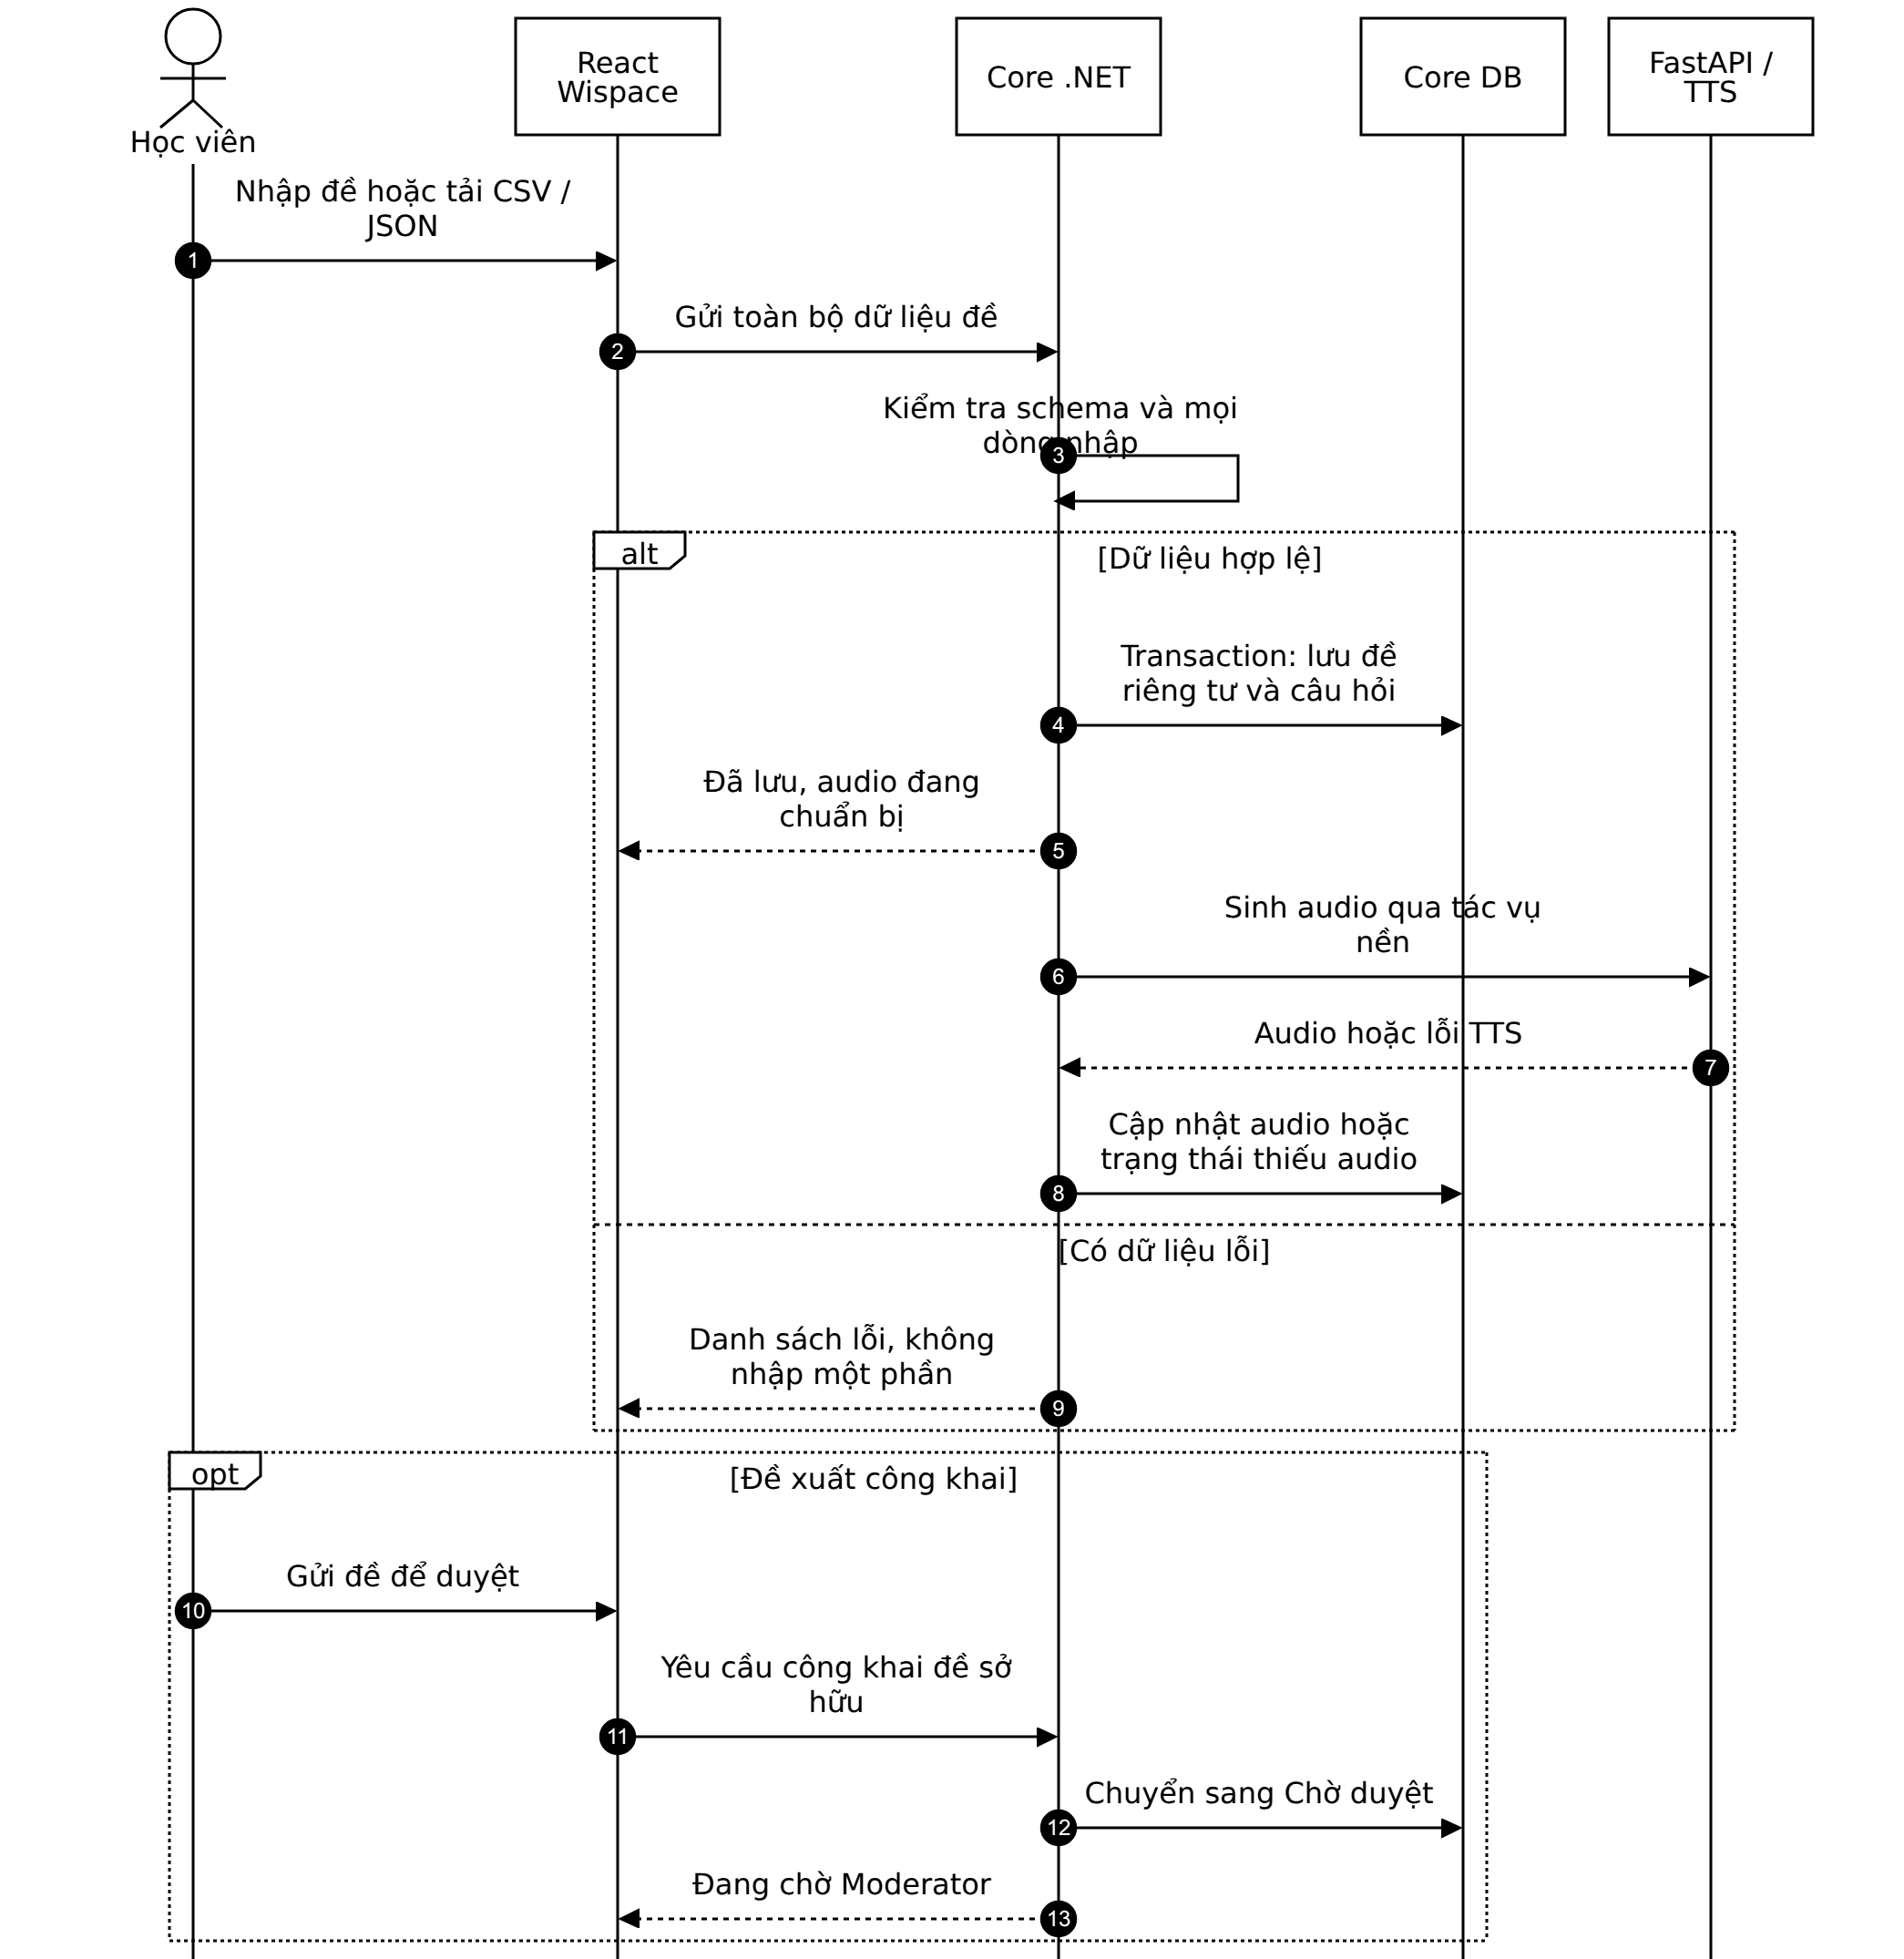
\includegraphics[width=\linewidth,height=.77\textheight,keepaspectratio]{Images/Sequence/Wispace/sequence_uc07_add_test.png}
\caption{Sequence diagram Wispace UC07 — Thêm đề luyện tập}
\label{sequence:wispace:sequence_uc07_add_test}
\end{figure}

Đề được lưu riêng tư sau kiểm tra toàn bộ; lỗi TTS không làm mất đề và đề xuất công khai cần kiểm duyệt.

\clearpage
\paragraph*{UC08. Quản lý và kiểm duyệt đề}

\begin{figure}[H]
\centering
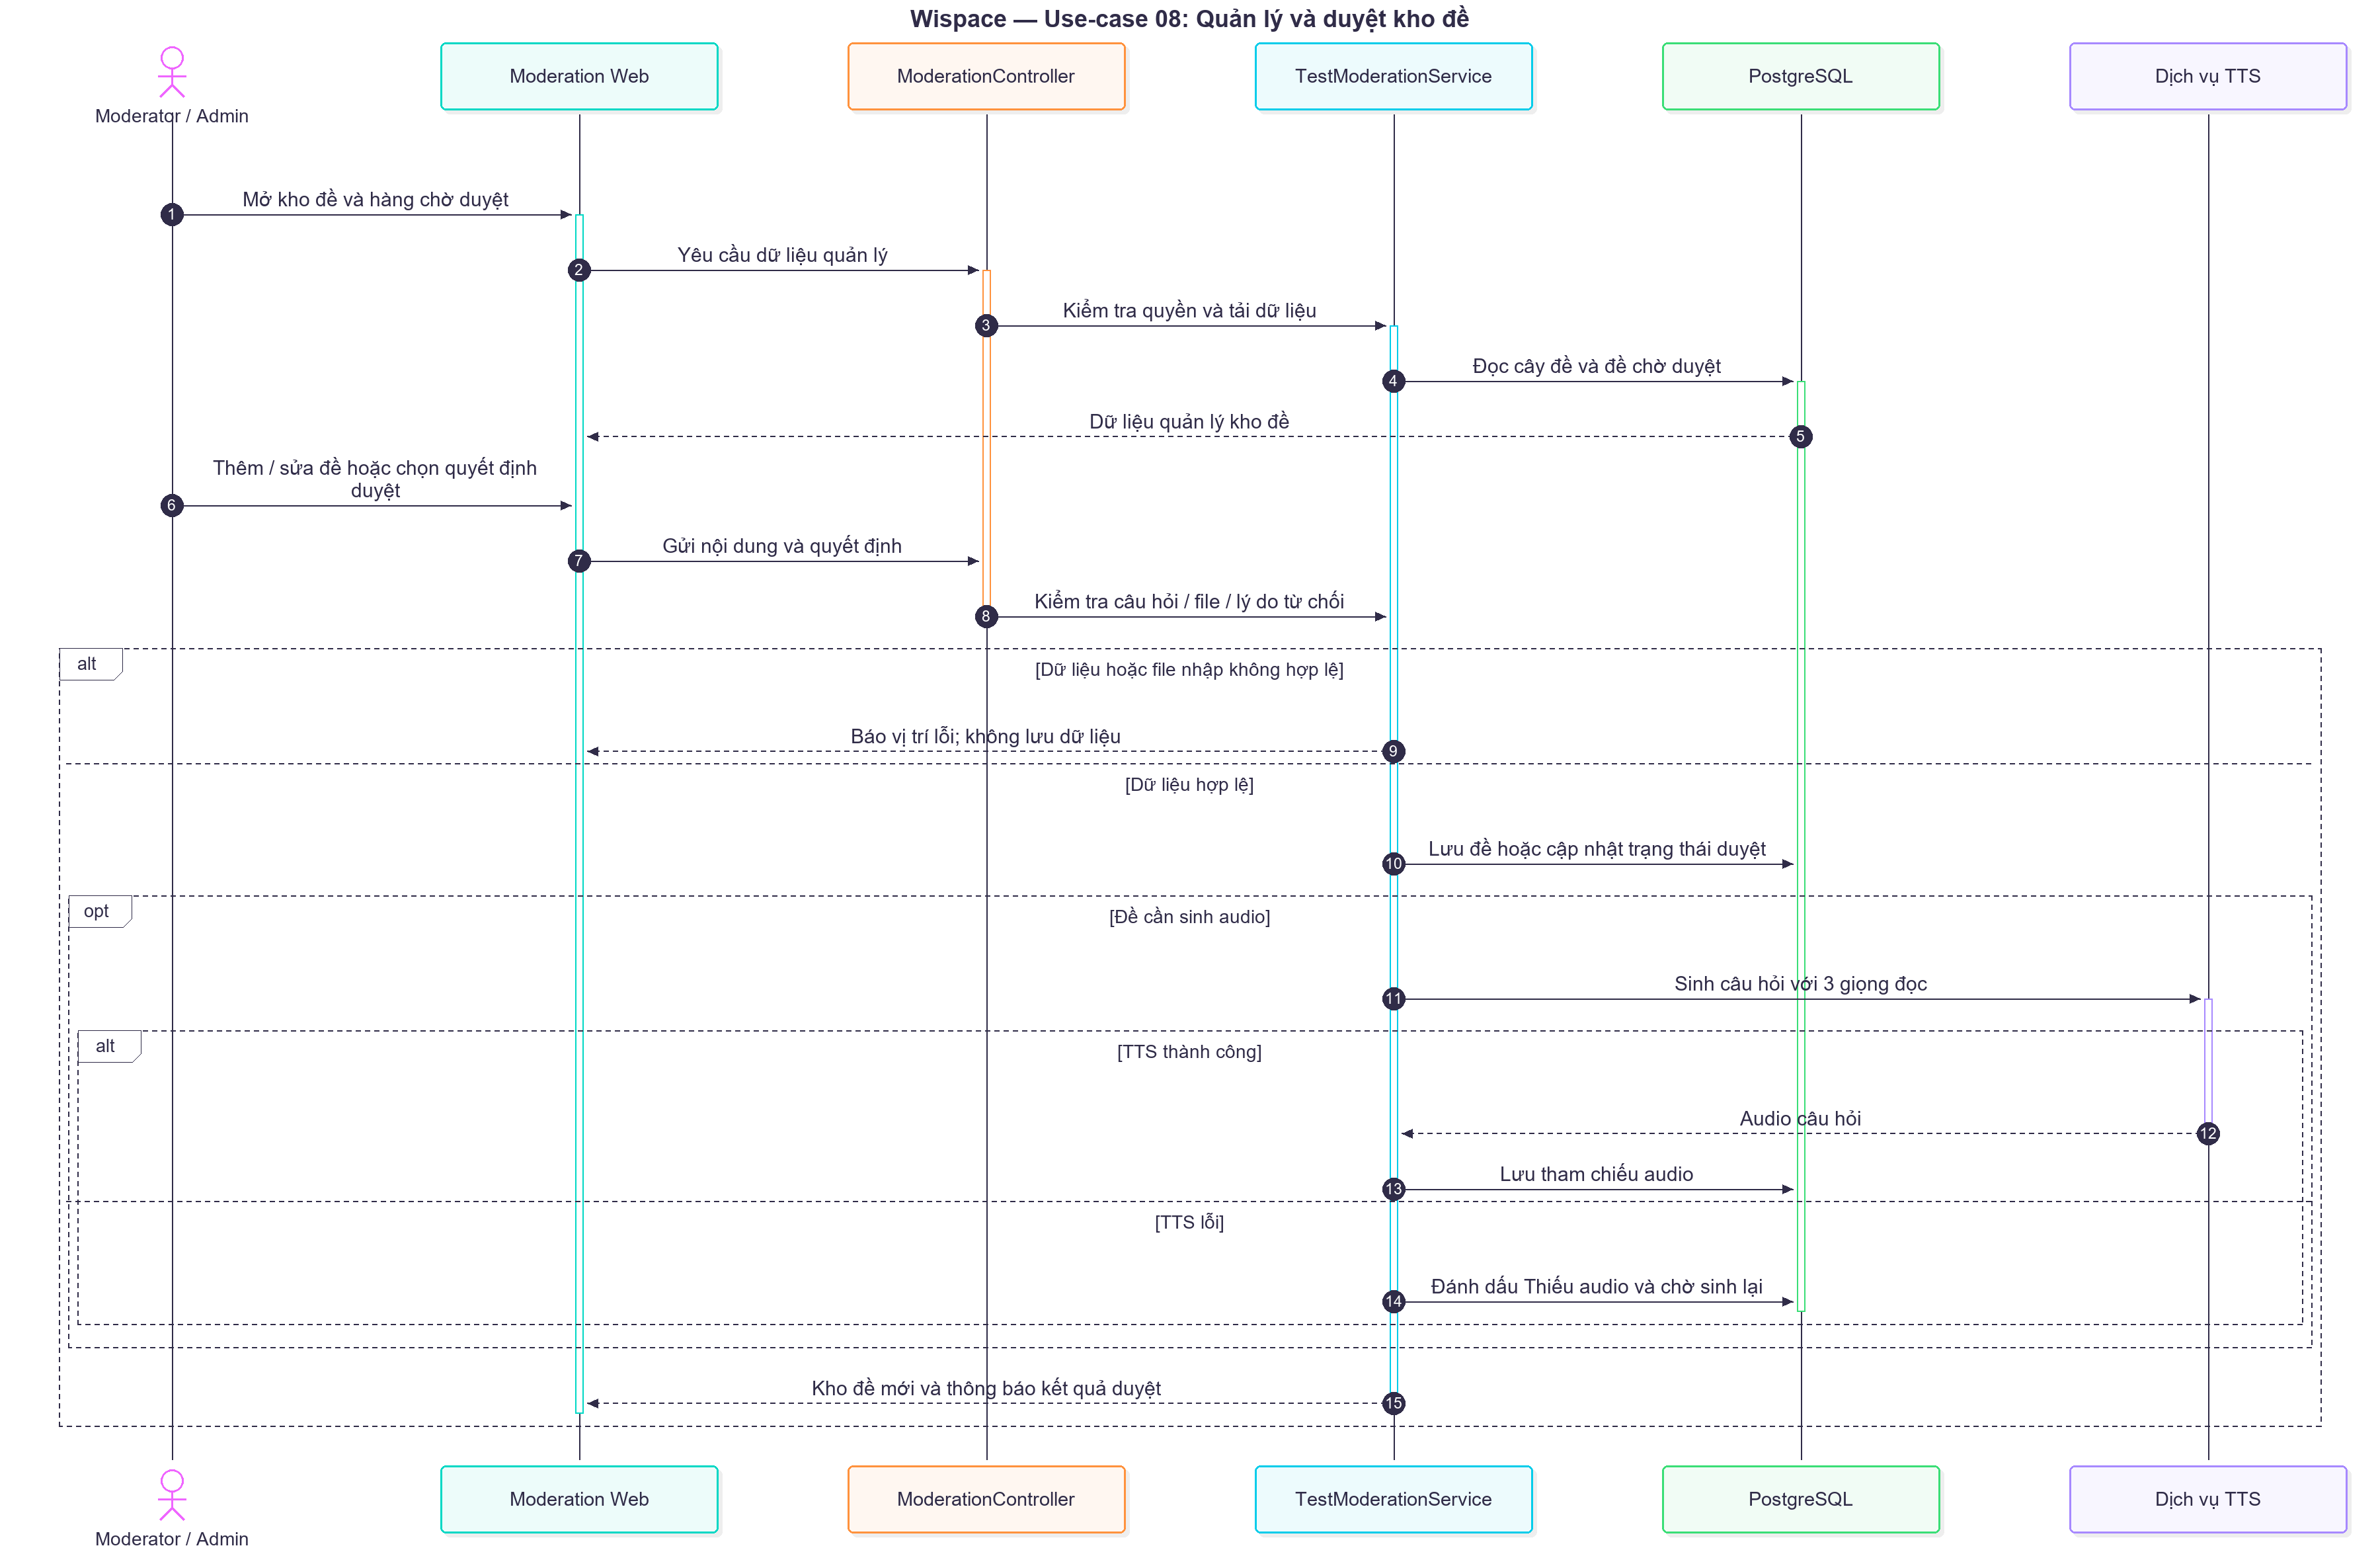
\includegraphics[width=\linewidth,height=.77\textheight,keepaspectratio]{Images/Sequence/Wispace/sequence_uc08_moderate_tests.png}
\caption{Sequence diagram Wispace UC08 — Quản lý và kiểm duyệt đề}
\label{sequence:wispace:sequence_uc08_moderate_tests}
\end{figure}

Quyết định duyệt sử dụng phiên bản để tránh ghi đè; ẩn đề bảo toàn lịch sử của người học.

\clearpage
\paragraph*{UC09. Luyện tập Speaking theo Part}

\begin{figure}[H]
\centering
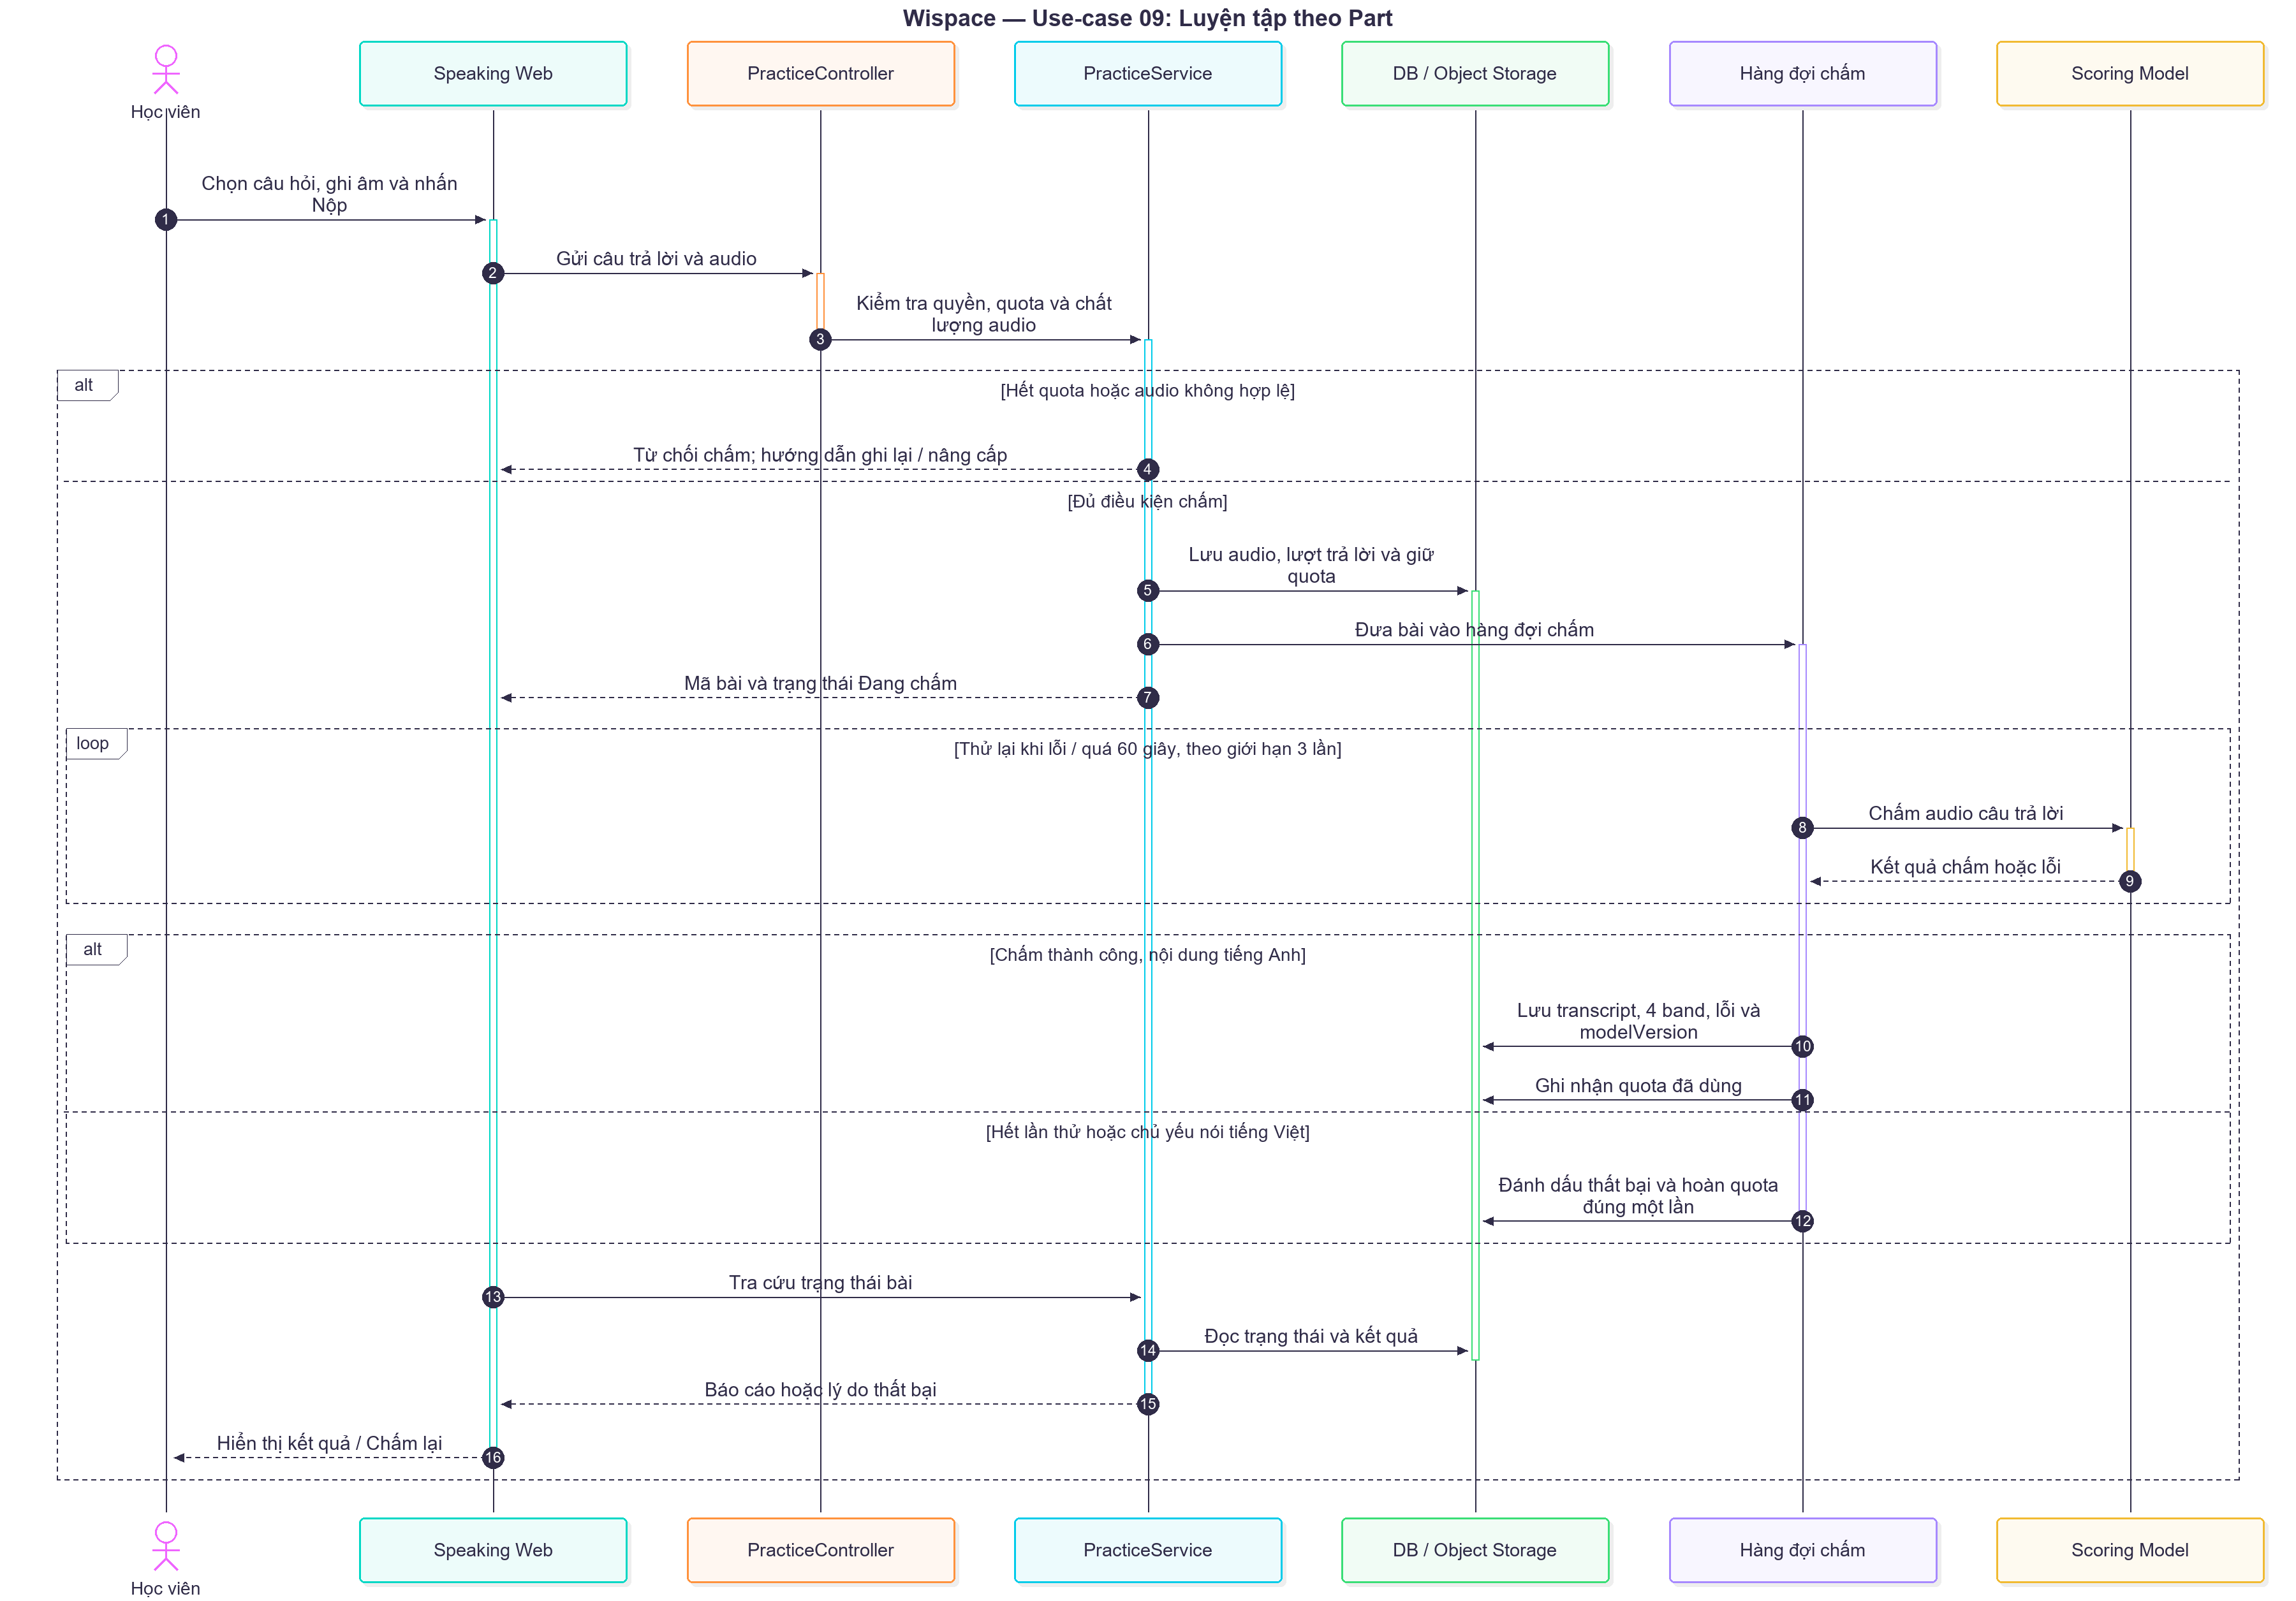
\includegraphics[width=\linewidth,height=.77\textheight,keepaspectratio]{Images/Sequence/Wispace/sequence_uc09_part_practice.png}
\caption{Sequence diagram Wispace UC09 — Luyện tập Speaking theo Part}
\label{sequence:wispace:sequence_uc09_part_practice}
\end{figure}

Learning, Core và Assessment dùng transaction riêng; sự kiện có outbox/inbox, quota không chốt trong transaction của Assessment.

\clearpage
\paragraph*{UC10. Xem kết quả và chấm lại}

\begin{figure}[H]
\centering
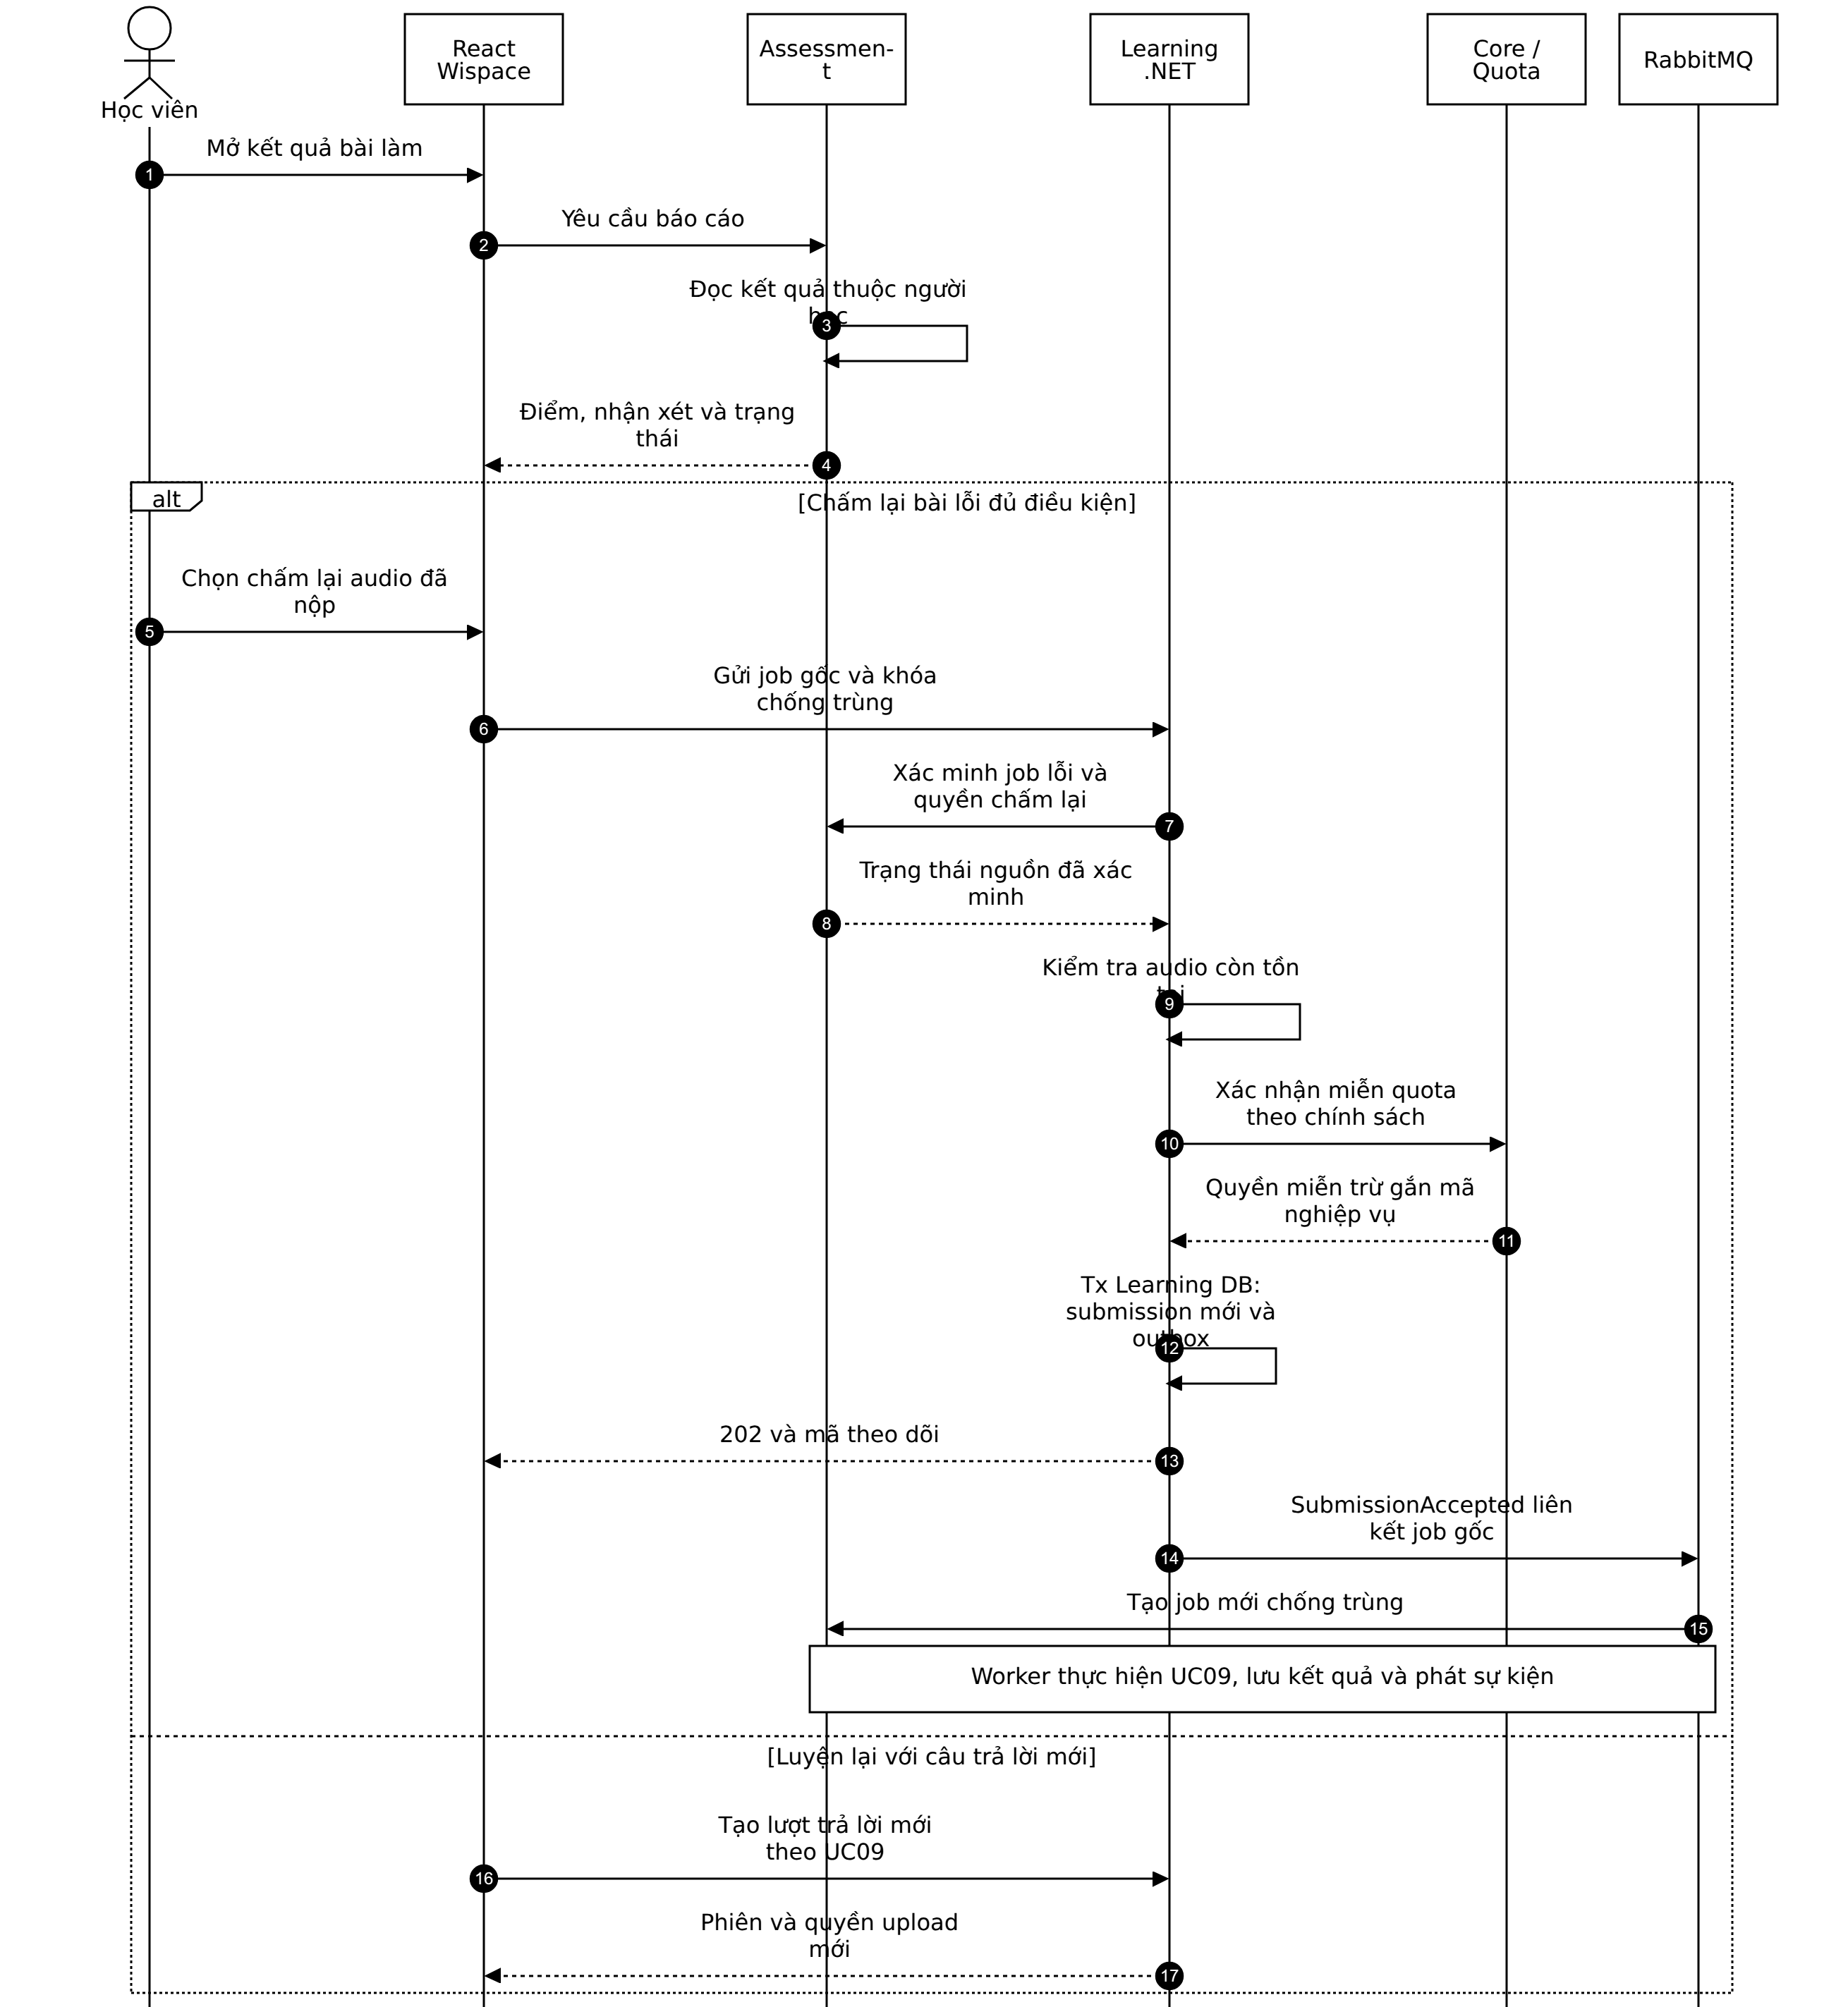
\includegraphics[width=\linewidth,height=.77\textheight,keepaspectratio]{Images/Sequence/Wispace/sequence_uc10_results_retry.png}
\caption{Sequence diagram Wispace UC10 — Xem kết quả và chấm lại}
\label{sequence:wispace:sequence_uc10_results_retry}
\end{figure}

Chấm lại lỗi phải xác minh miễn quota và audio; lượt luyện mới tạo submission mới, không cập nhật trực tiếp sổ Core.

\clearpage
\paragraph*{UC11. Thi thử Speaking}

\begin{figure}[H]
\centering
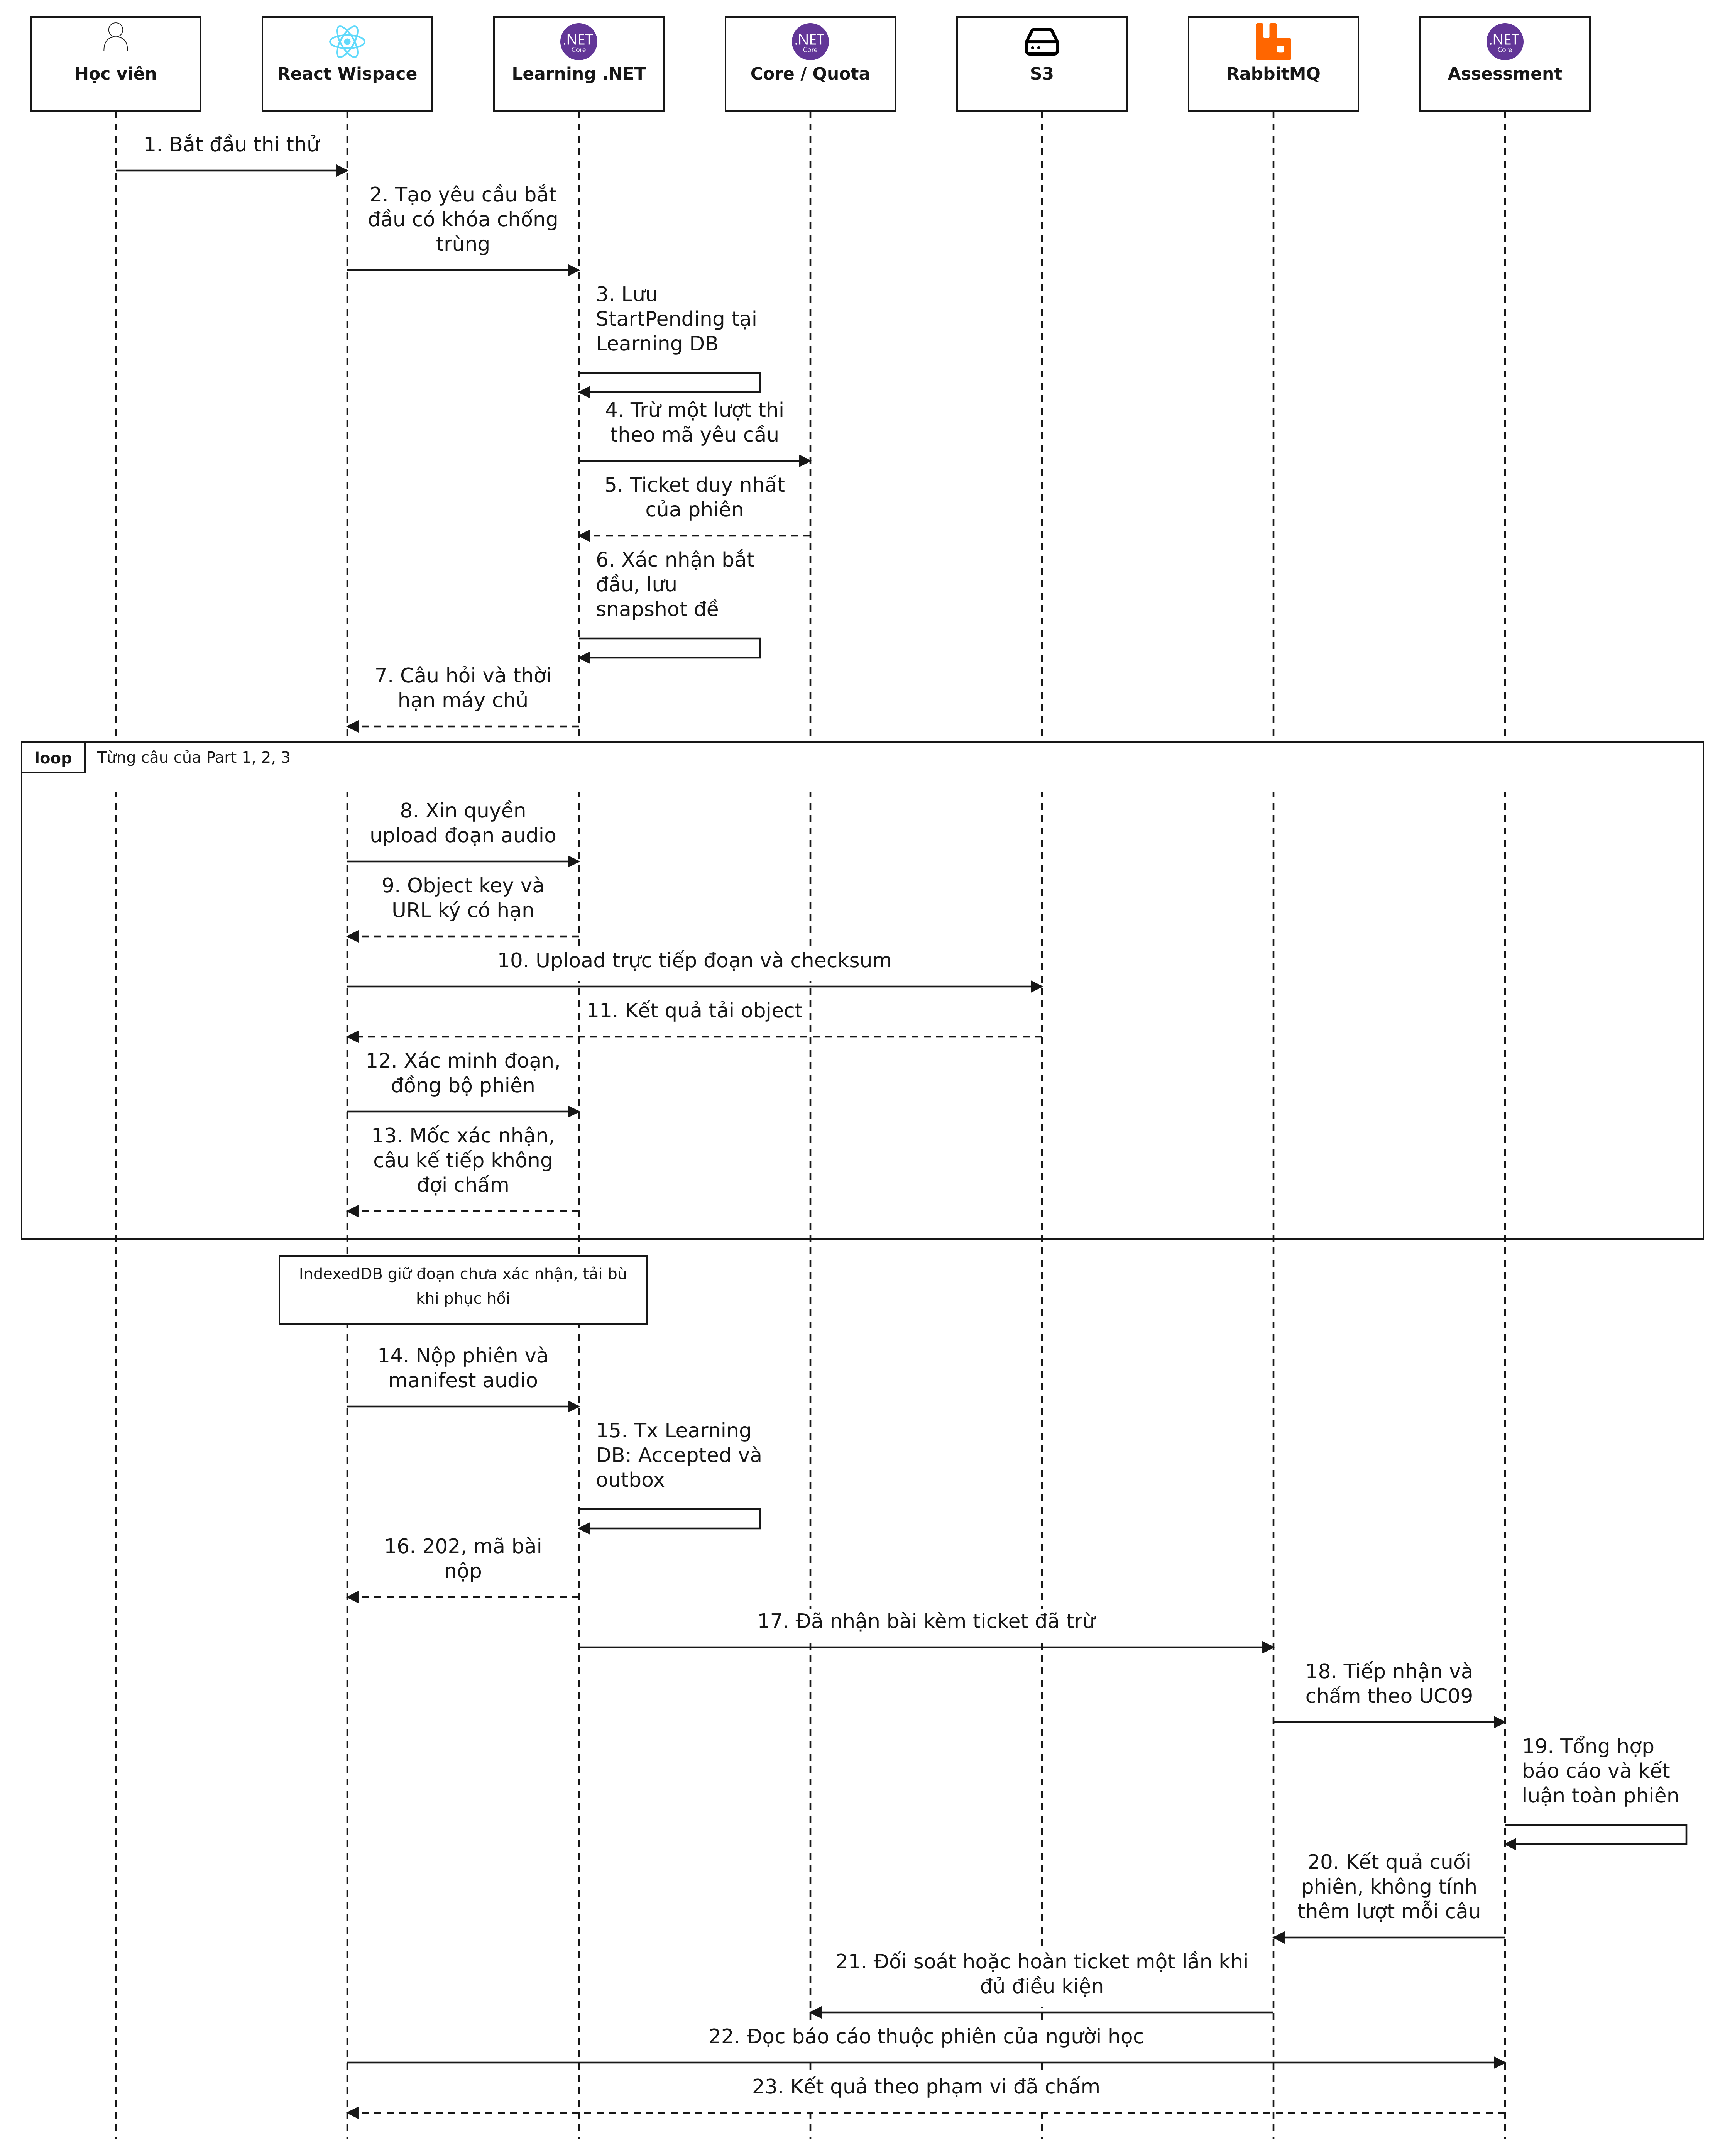
\includegraphics[width=\linewidth,height=.77\textheight,keepaspectratio]{Images/Sequence/Wispace/sequence_uc11_mock_test.png}
\caption{Sequence diagram Wispace UC11 — Thi thử Speaking}
\label{sequence:wispace:sequence_uc11_mock_test}
\end{figure}

Audio đi trực tiếp vào Object Storage; Core trừ một lượt theo ticket, Assessment kết luận toàn phiên trước khi phát quyết định hoàn.

\clearpage
\paragraph*{UC12. Lịch sử và theo dõi tiến bộ}

\begin{figure}[H]
\centering
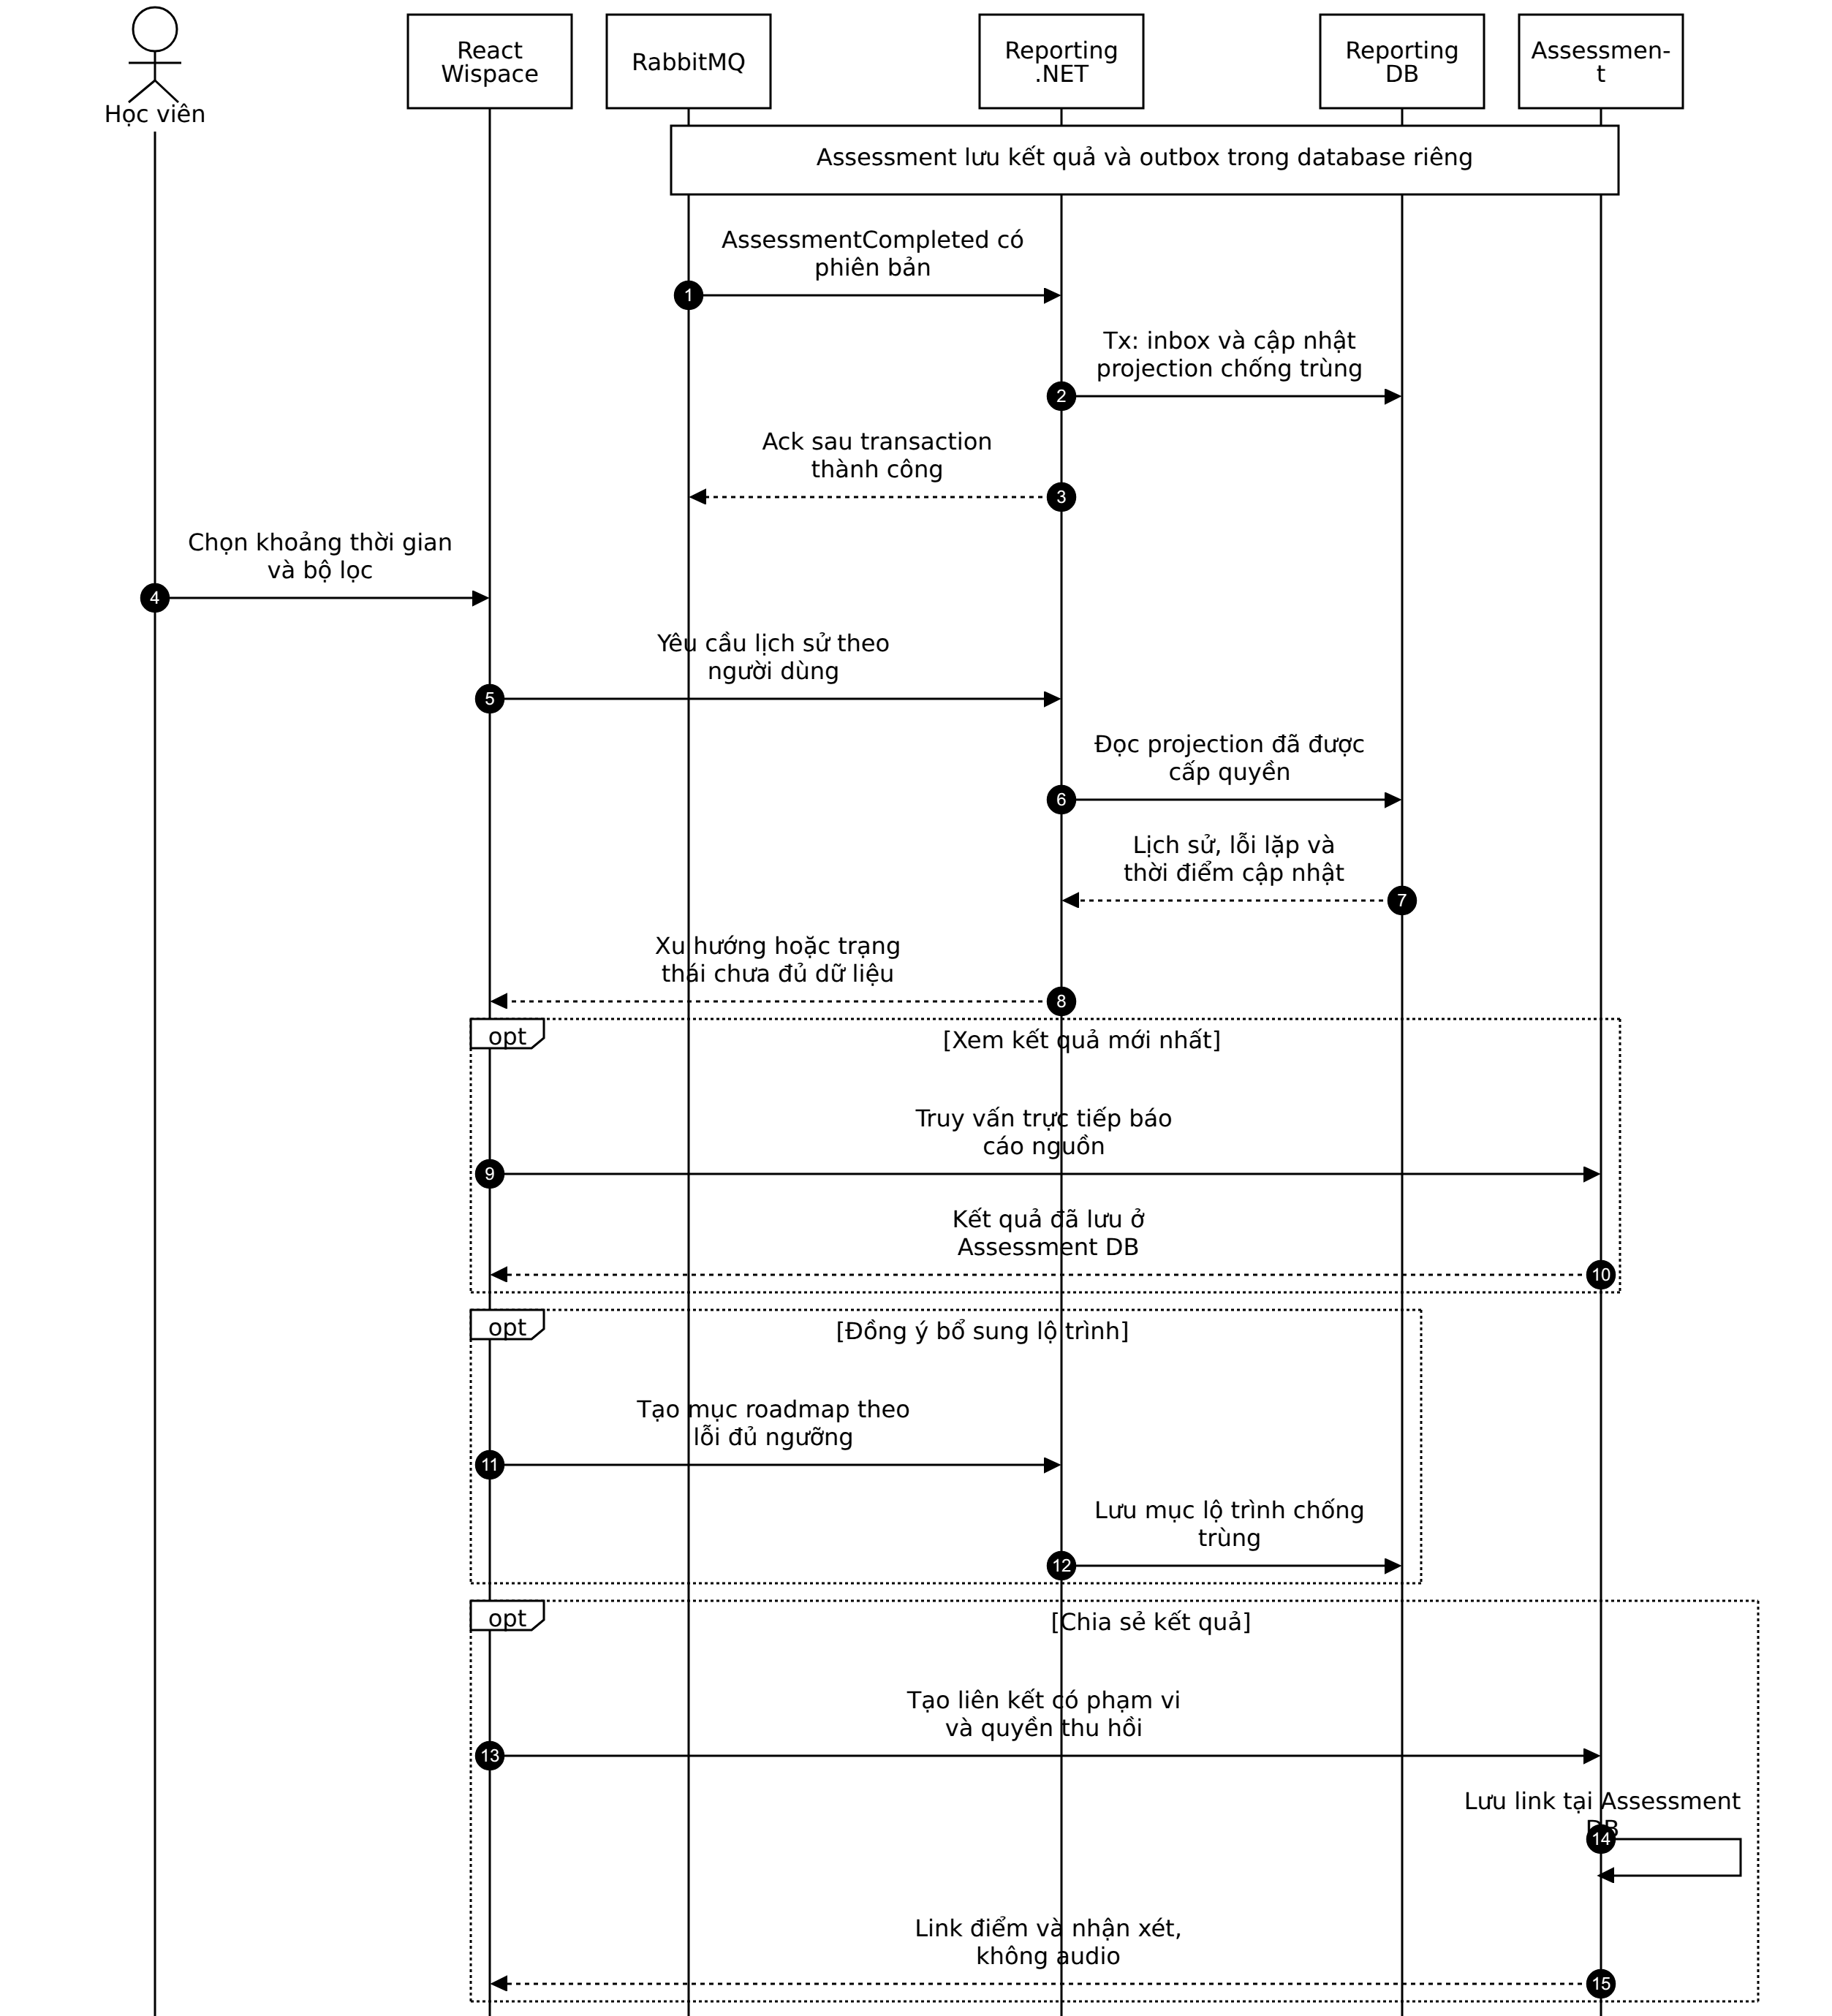
\includegraphics[width=\linewidth,height=.77\textheight,keepaspectratio]{Images/Sequence/Wispace/sequence_uc12_progress_history.png}
\caption{Sequence diagram Wispace UC12 — Lịch sử và theo dõi tiến bộ}
\label{sequence:wispace:sequence_uc12_progress_history}
\end{figure}

Reporting đọc database tổng hợp riêng, hiển thị độ mới dữ liệu; báo cáo nguồn và liên kết chia sẻ thuộc Assessment.

\subsubsection{Bảo mật và vận hành riêng của Wispace}

Quyền truy cập bài làm, audio và kết quả được kiểm tra theo chủ sở hữu tại backend. Moderator được kiểm duyệt kho đề nhưng không mặc nhiên được nghe audio riêng tư của học viên. Link chia sẻ chỉ công bố điểm và nhận xét trong phạm vi được cho phép; học viên có thể thu hồi link.

Luồng chấm dùng queue speaking.assessment và Assessment Worker có giới hạn đồng thời. Kết quả, quota và trạng thái phiên được cập nhật bằng transaction riêng tại dịch vụ sở hữu, kết nối bằng outbox/inbox và cơ chế đối soát. Thông báo SignalR chỉ gửi đến người được phép; khi mất kết nối, giao diện đọc lại trạng thái bằng REST. Audio có vòng đời 180 ngày; xóa audio không làm mất điểm và transcript được phép giữ.

\subsection{Thiết kế hệ thống AIHub}

\subsubsection{Phạm vi, giao diện và kiến trúc}

AIHub là hệ thống quản lý và cung cấp API mô hình cho các tổ chức B2B. Frontend React AIHub phục vụ Portal đối tác, quản trị nền tảng và khu vực Academic Lab nội bộ. Ứng dụng máy chủ của đối tác gọi API B2B trên .NET; Gateway xác thực credentials, kiểm tra quyền dịch vụ và điều phối tới Python FastAPI qua adapter được cấu hình.

AIHub có thể cung cấp cùng mô hình Speaking mà Wispace đang sử dụng, nhưng yêu cầu đối tác có danh tính tổ chức, quota và nhật ký riêng. Các dịch vụ sinh bài tập, Prompt, dẫn chứng và xuất dữ liệu thuộc công cụ chất lượng mô hình; khách B2B không tự động có quyền truy cập dữ liệu Academic Lab.

\paragraph*{Tổ chức frontend}

Frontend AIHub có ba khu vực chức năng:

\begin{enumerate}
\item \textbf{Portal khách hàng B2B:} tổ chức, thành viên, credentials, danh mục API, tài liệu tích hợp, Sandbox, hạn mức và usage.
\item \textbf{Quản trị nền tảng:} danh mục mô hình, model route, gói B2B, cấu hình dịch vụ và giám sát.
\item \textbf{Academic Lab nội bộ:} mẫu sinh, bản hiệu đính, điểm chất lượng, quyết định duyệt và xuất dữ liệu.
\end{enumerate}

Việc tách route trên React giúp tổ chức giao diện. Backend phải kiểm tra quyền độc lập tại từng endpoint; ẩn nút hoặc chặn route phía trình duyệt không thay thế kiểm soát truy cập trên máy chủ.

\begin{figure}[H]
\centering
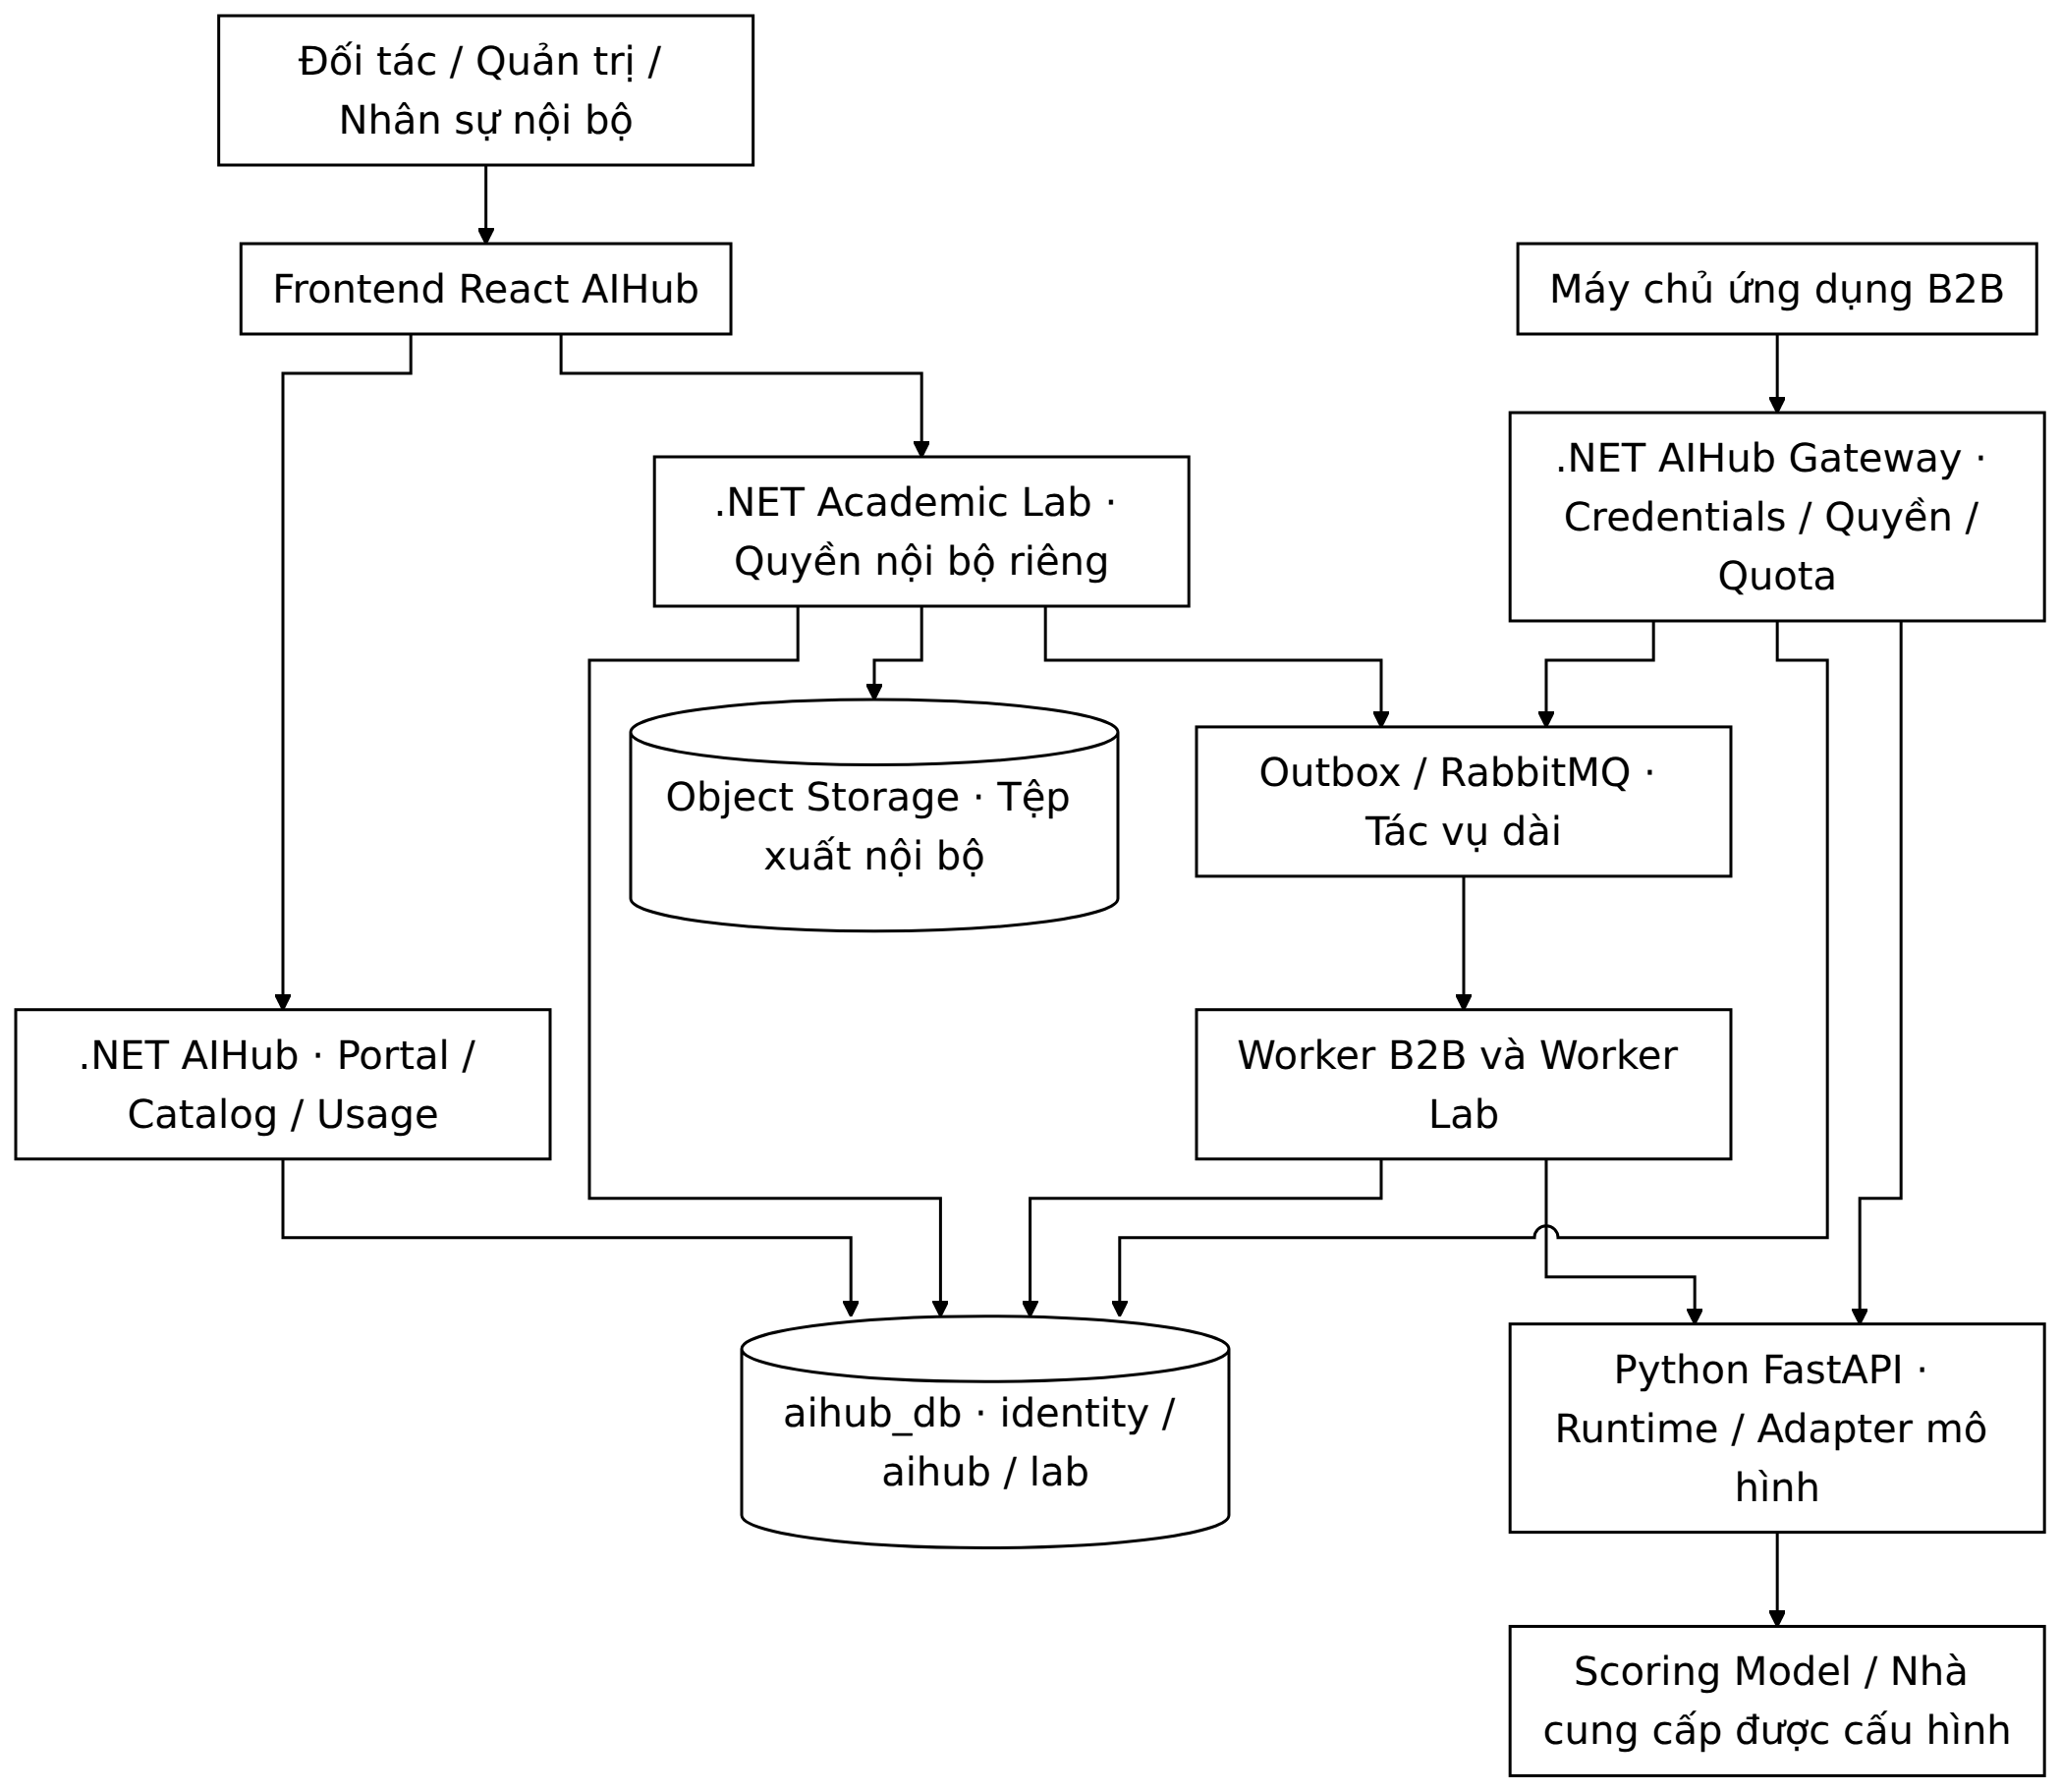
\includegraphics[width=\linewidth,height=.72\textheight,keepaspectratio]{Images/Design/aihub_architecture.png}
\caption{Kiến trúc chức năng của AIHub}
\label{design:fig:aihub_architecture}
\end{figure}

\paragraph*{Các module xử lý}

\begingroup\small\setstretch{1.1}
\begin{longtable}{|>{\raggedright\arraybackslash}p{\dimexpr 0.29\linewidth-2\tabcolsep-2\arrayrulewidth\relax}|>{\raggedright\arraybackslash}p{\dimexpr 0.71\linewidth-2\tabcolsep-2\arrayrulewidth\relax}|}
\caption{Các module xử lý}\label{design:tab:2}\\
\hline
\textbf{Module} & \textbf{Trách nhiệm} \\ \hline
\endfirsthead
\hline
\textbf{Module} & \textbf{Trách nhiệm} \\ \hline
\endhead
\endfoot
AIHub.Access & Tổ chức, thành viên, credentials và quyền dùng dịch vụ. \\ \hline
AIHub.Gateway & Xác thực B2B, kiểm định yêu cầu, điều phối thực thi và chuẩn hóa phản hồi. \\ \hline
AIHub.Catalog & Danh mục API, Universal Specs, phiên bản mô hình, model route và Sandbox. \\ \hline
AIHub.Usage & Gói tổ chức, rate limit, quota, usage và đối soát. \\ \hline
AcademicLab & Dẫn chứng, sinh mẫu, hiệu đính, thẩm định, xuất dữ liệu và phân tích chất lượng. \\ \hline
\end{longtable}
\endgroup

\subsubsection{Thiết kế dữ liệu AIHub}

\begin{figure}[H]
\centering
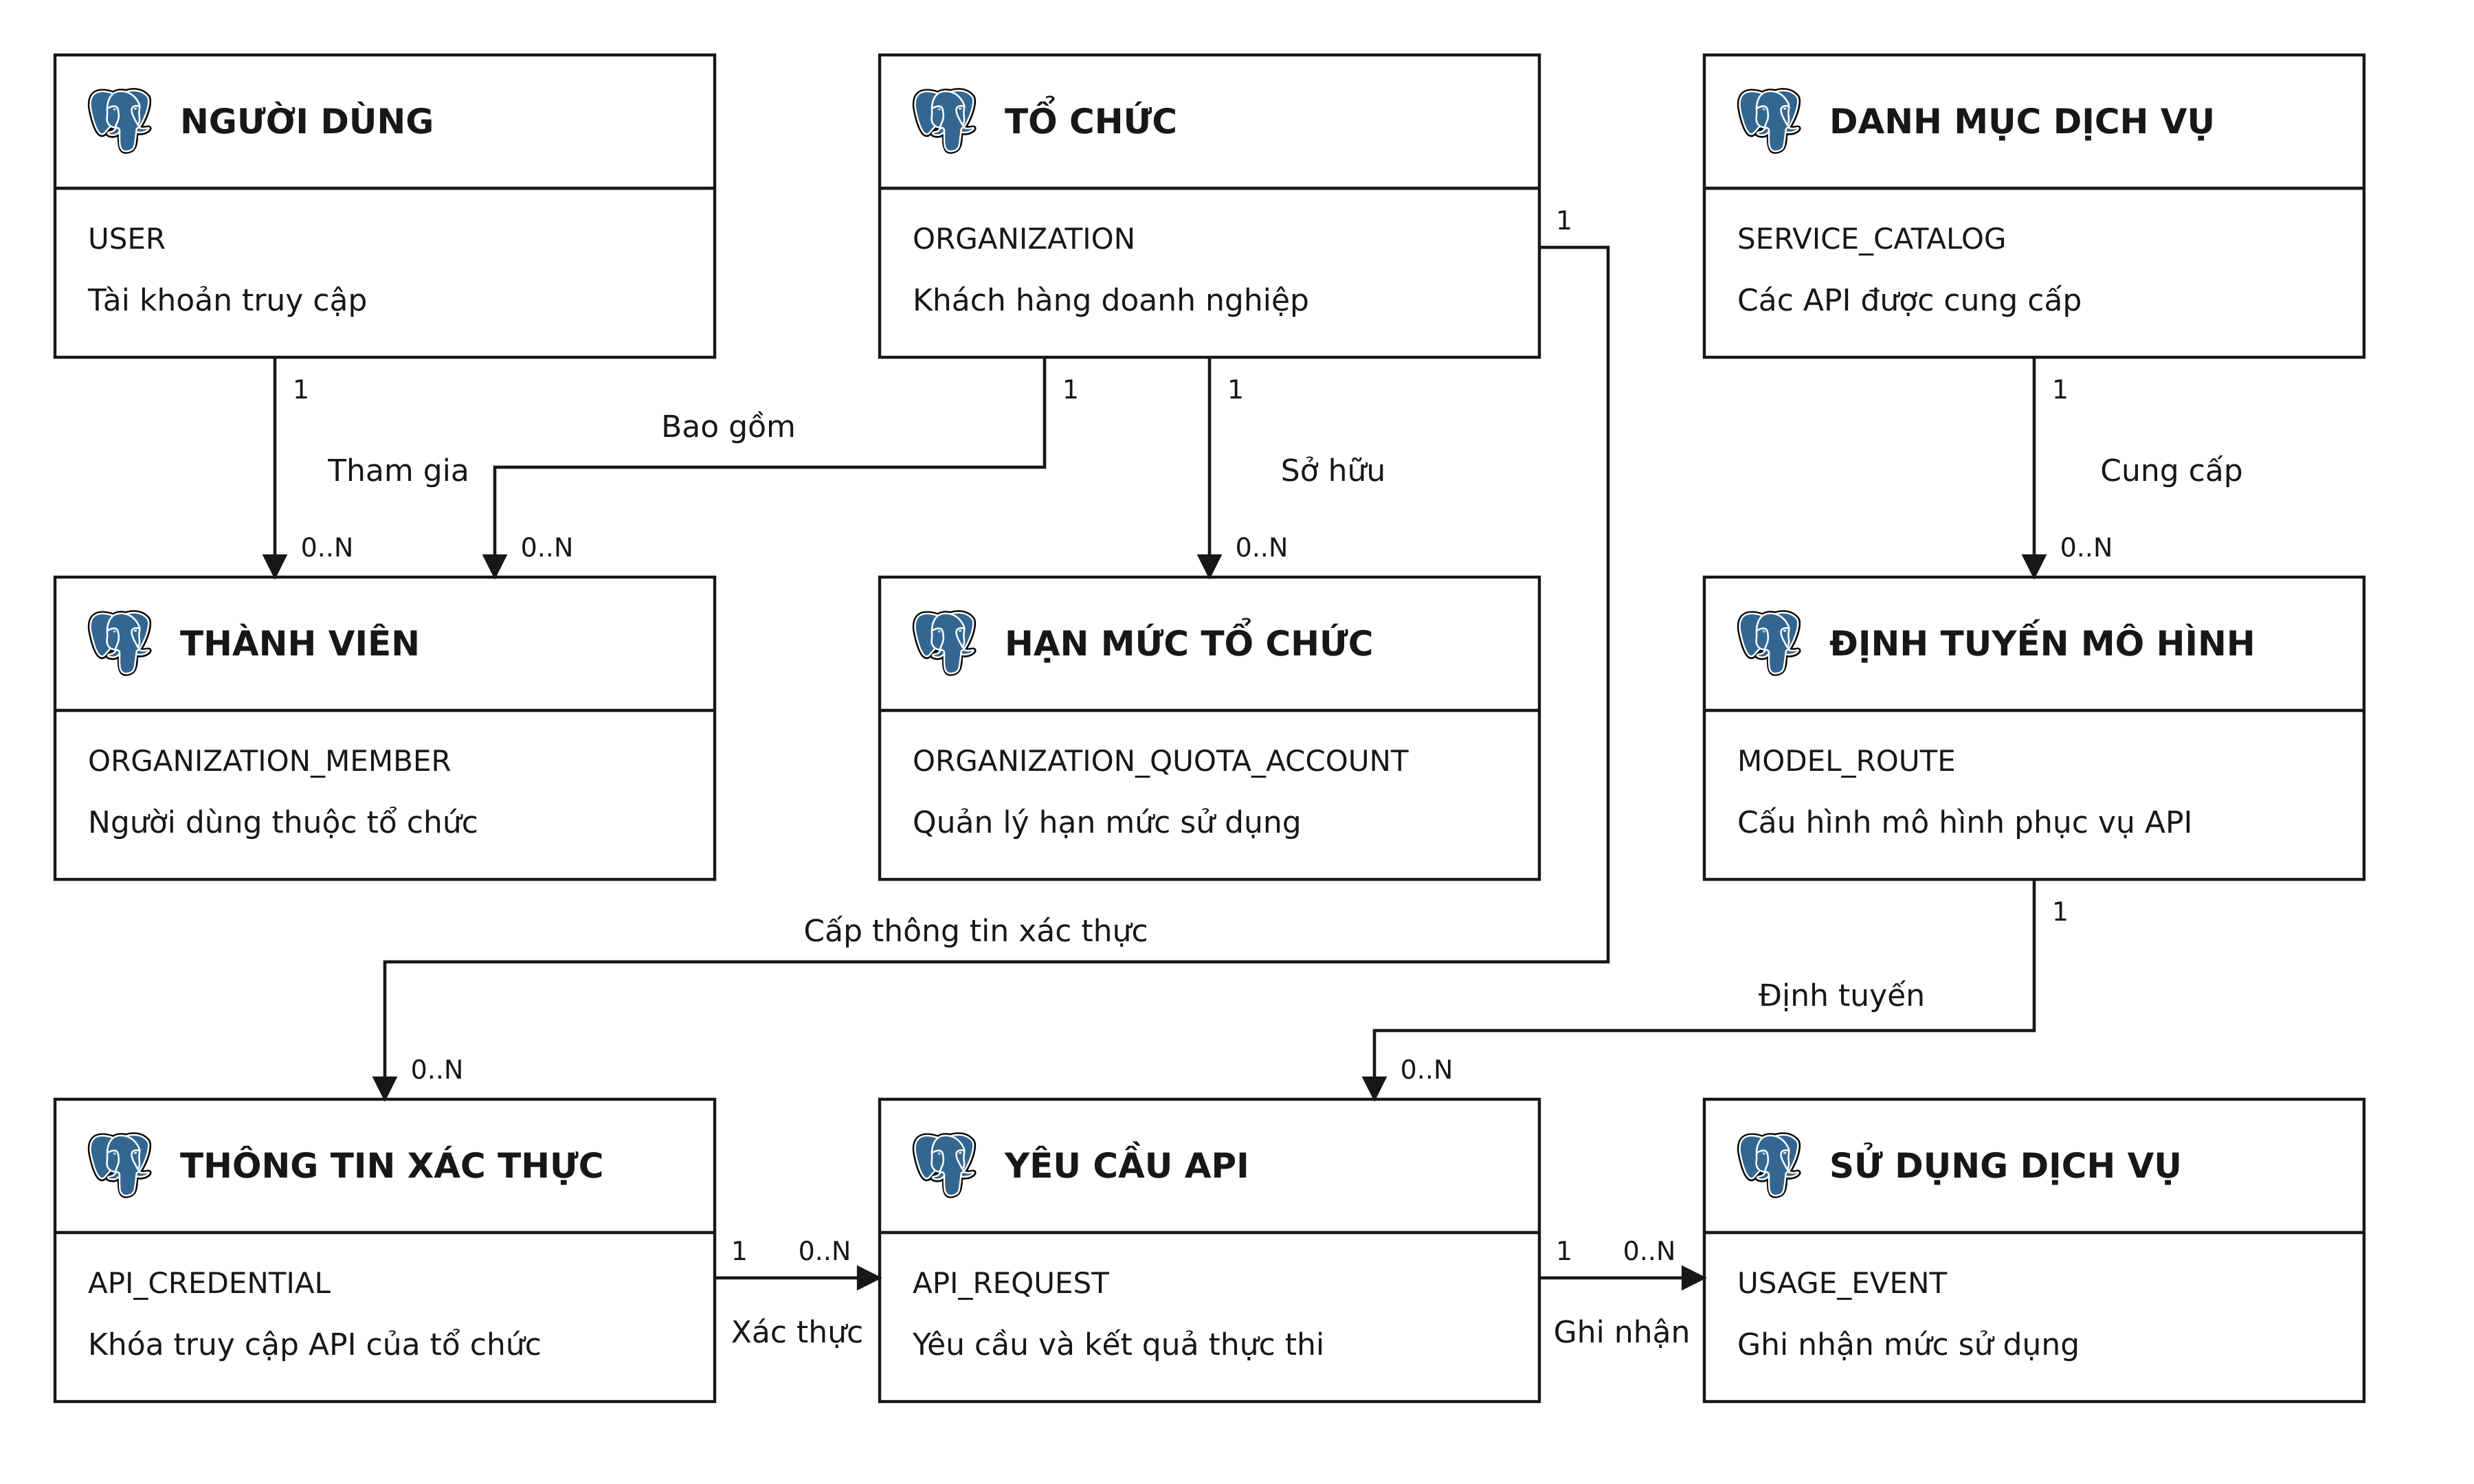
\includegraphics[width=\linewidth,height=.72\textheight,keepaspectratio]{Images/Design/aihub_data.png}
\caption{Quan hệ dữ liệu chính của AIHub B2B}
\label{design:fig:aihub_data}
\end{figure}

\begin{figure}[H]
\centering
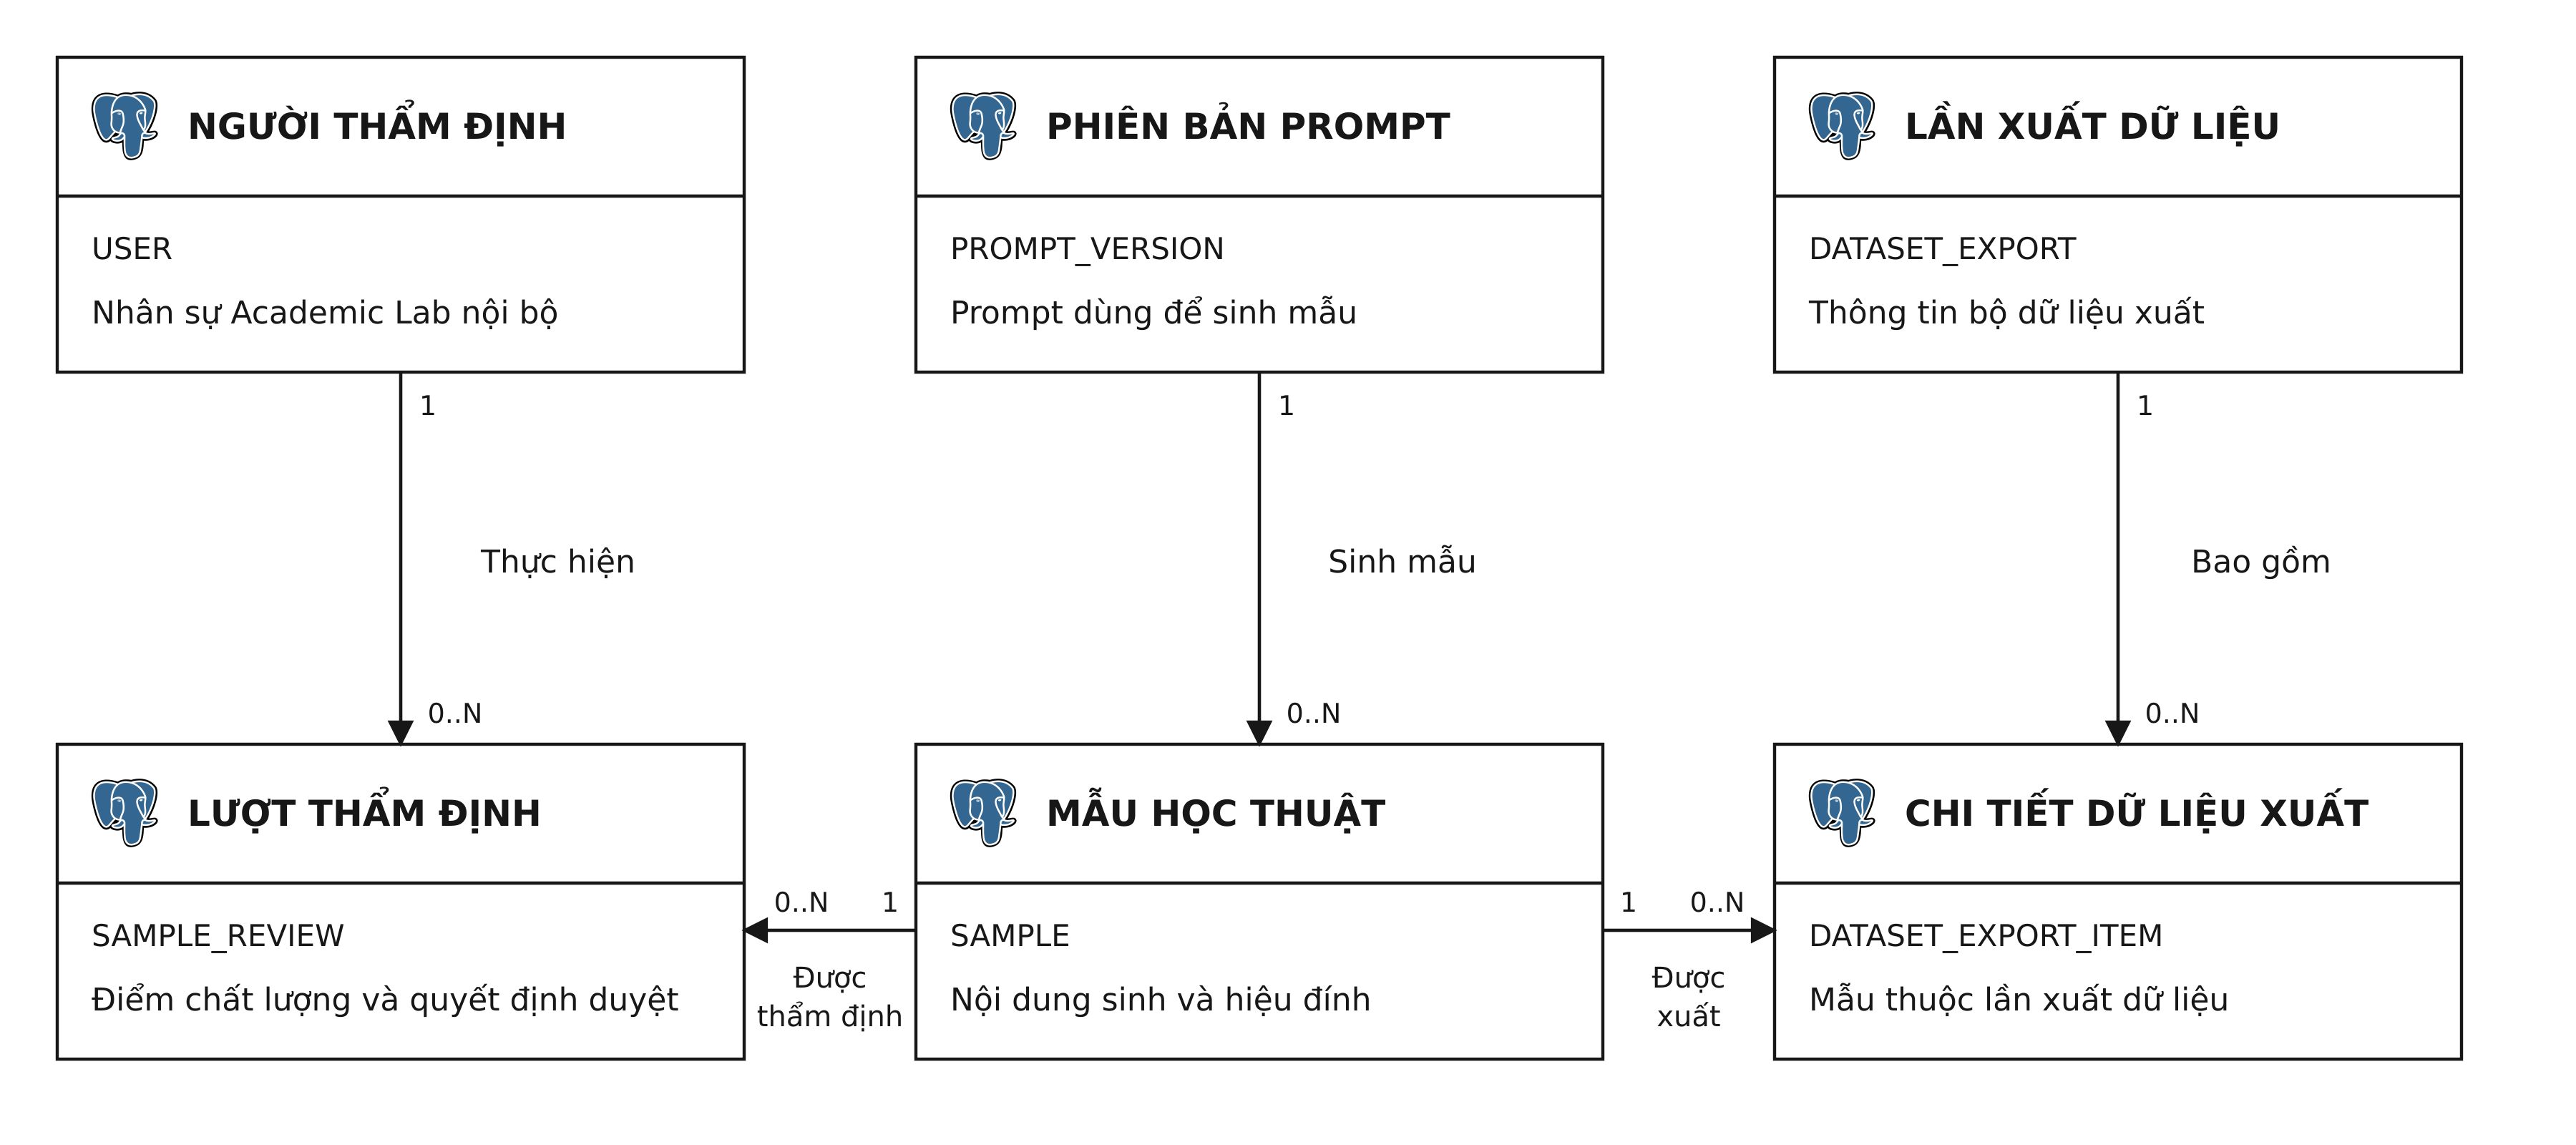
\includegraphics[width=\linewidth,height=.72\textheight,keepaspectratio]{Images/Design/lab_data.png}
\caption{Quan hệ dữ liệu Academic Lab nội bộ}
\label{design:fig:lab_data}
\end{figure}

Một người dùng có thể tham gia nhiều tổ chức. Quyền của thành viên được đánh giá theo tổ chức đang thao tác. Quyền nội bộ của Academic Lab được cấp riêng; việc sở hữu một tổ chức hoặc API key không tạo quyền đọc mẫu, audio hay dữ liệu huấn luyện nội bộ.

Metadata công việc B2B được lưu theo \texttt{api\allowbreak{}Request\allowbreak{}Id} và \texttt{organization\allowbreak{}Id}; những lần thử cần được lưu với route, phiên bản mô hình thực tế, thời gian và lỗi tương ứng. Số liệu chi phí mỗi lần suy luận được tách khỏi số lần tiêu thụ hạn mức nghiệp vụ. Tệp xuất của Academic Lab có manifest riêng, được lưu trong bucket nội bộ với quyền truy cập có thời hạn.

\subsubsection{Thiết kế API B2B và quản lý mô hình}

\paragraph*{Danh mục dịch vụ và quyền khai thác}

AIHub công bố danh mục dịch vụ gồm mã dịch vụ, phiên bản API, schema đầu vào/đầu ra, hình thức xử lý đồng bộ hoặc bất đồng bộ, model route được phép và đơn vị tính hạn mức. Một tổ chức chỉ được gọi các dịch vụ đã được cấp quyền trong gói của mình.

Danh mục có thể bao gồm chấm Speaking hoặc các tác vụ AI khác nếu được cấu hình công khai cho đối tác. Việc công bố cùng một Scoring Model qua B2B không làm thay đổi đường gọi AI trực tiếp của module Wispace. API công khai không cho đối tác truyền tùy ý URL nội bộ, tên container hay địa chỉ nhà cung cấp để backend gọi theo.

\paragraph*{Luồng tiếp nhận API B2B}

\begin{figure}[H]
\centering
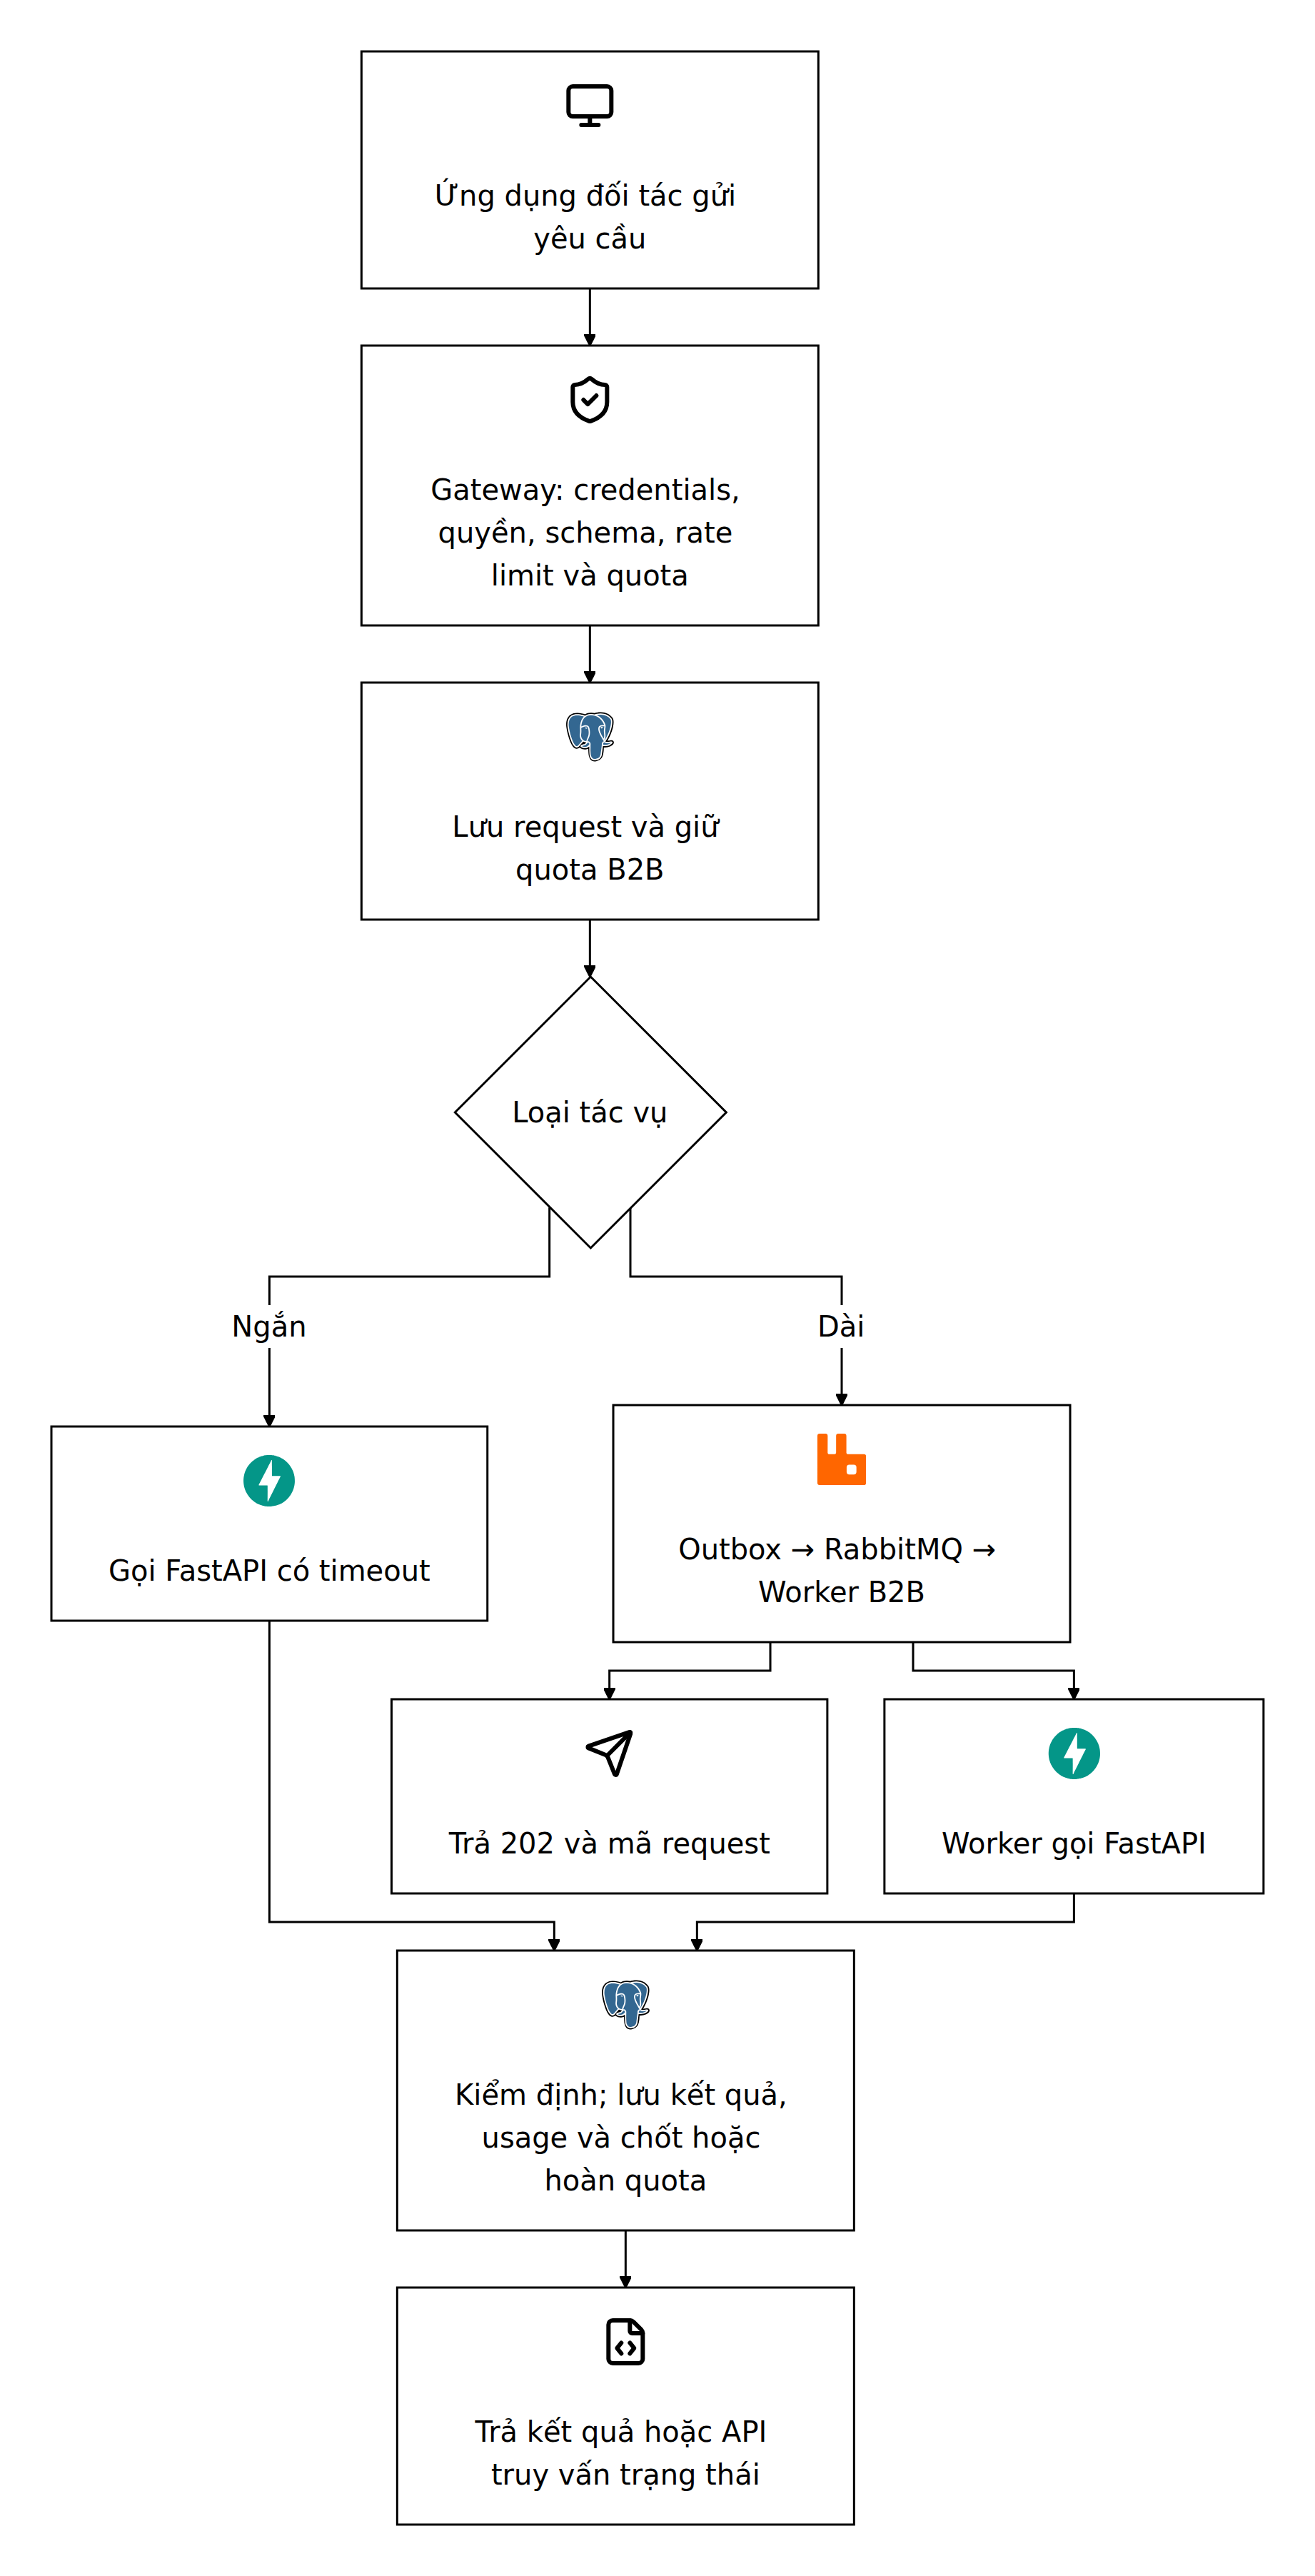
\includegraphics[width=\linewidth,height=.72\textheight,keepaspectratio]{Images/Design/b2b_flow.png}
\caption{Luồng tiếp nhận API B2B}
\label{design:fig:b2b_flow}
\end{figure}

Các tác vụ dài như chấm audio được xử lý bất đồng bộ. Đối tác nhận mã yêu cầu và dùng endpoint truy vấn trạng thái trong phạm vi tổ chức. Những tác vụ ngắn có thể dùng phản hồi đồng bộ với timeout phù hợp. Nếu client gửi lại do mất phản hồi, \texttt{Idempotency-\allowbreak{}Key} và nội dung yêu cầu phải được kiểm tra để tránh tạo yêu cầu và tính hạn mức lặp.

\paragraph*{Credentials và phân quyền tổ chức}

Mỗi bộ credentials có \texttt{client\allowbreak{}Id}, bí mật ngẫu nhiên, môi trường sử dụng, tập quyền dịch vụ, thời điểm tạo và trạng thái. Bí mật chỉ hiển thị một lần khi cấp mới hoặc xoay vòng; hệ thống lưu dạng băm và không cung cấp endpoint đọc lại bí mật gốc.

Đề xuất giữ cách xác thực \texttt{x-\allowbreak{}client-\allowbreak{}id} và \texttt{x-\allowbreak{}secret-\allowbreak{}key} đã được mô tả trong yêu cầu. Credentials được dùng qua HTTPS từ ứng dụng máy chủ của đối tác; không nhúng bí mật B2B vào mã JavaScript công khai. Sau xác thực, \texttt{organization\allowbreak{}Id} được suy ra từ khóa đã lưu, thay vì tin trực tiếp định danh tổ chức trong request body.

Quản trị viên tổ chức có thể quản lý credentials và thành viên trong phạm vi quyền được cấp. Quản trị viên nền tảng mới được công bố dịch vụ, đổi cấu hình model route hoặc thay đổi chính sách gói toàn cục. Khóa bị thu hồi phải bị từ chối ở các yêu cầu tiếp theo theo kiểm tra trạng thái có thẩm quyền; cache xác thực không được làm vô hiệu thao tác thu hồi.

\paragraph*{Rate limit, quota và usage}

Rate limit giới hạn tốc độ truy cập trong một khoảng ngắn; quota giới hạn lượng sử dụng theo gói và chu kỳ. Mỗi dịch vụ định nghĩa đơn vị tiêu thụ, ví dụ lượt gọi hoặc thời lượng audio. Việc kiểm tra và giữ quota được thực hiện nguyên tử để các yêu cầu đồng thời không cùng tiêu thụ một số dư.

Thiết kế đề xuất chốt hạn mức nghiệp vụ khi kết quả được lưu thành công; lỗi hệ thống cuối cùng giải phóng phần đang giữ. Các chi phí thực tế của nhà cung cấp, kể cả chi phí phát sinh ở lần thử lỗi, được ghi riêng cho vận hành. Rate limit vẫn ghi nhận lần truy cập để ngăn việc gửi lặp gây quá tải.

Yêu cầu đồng bộ cũng có trạng thái và thời hạn xử lý trong PostgreSQL. Nếu API host dừng giữa lúc gọi mô hình và lưu kết quả, tác vụ đối soát phát hiện yêu cầu quá hạn, kiểm tra kết quả theo định danh khi dịch vụ hỗ trợ, rồi kết thúc hoặc khôi phục theo chính sách. Không tự động gọi lại dịch vụ có tính phí khi chưa xác định hành vi chống lặp; kết quả muộn chỉ được chấp nhận khi yêu cầu vẫn còn quyền hoàn tất. Mọi khoản giữ hạn mức phải được chốt hoặc giải phóng bằng thao tác có kiểm tra chống lặp.

Mỗi usage event chứa tổ chức, credentials, dịch vụ, phiên bản mô hình, request ID, trạng thái, latency và đơn vị tiêu thụ. Với dịch vụ LLM có thể ghi token; với Scoring Model cần ghi thời lượng audio và thời gian suy luận tương ứng. Phân biệt số liệu đo được với chi phí ước tính theo bảng giá cấu hình.

\paragraph*{Chọn mô hình và xử lý dự phòng}

Mỗi loại dịch vụ có chính sách model route riêng. Dịch vụ sinh bài hoặc sinh nội dung có thể sử dụng chuỗi WISPACE Micro-Engine, Gemini, OpenAI và phương án xác định theo cấu hình của đề tài. Đầu ra dự phòng phải được kiểm định theo cùng hợp đồng; phản hồi ghi rõ mô hình thực tế đã sử dụng.

Đối với chấm Speaking, phương án khôi phục là chuyển tới bản sao hoặc phiên bản Scoring Model đã được kiểm chứng, hoặc giữ công việc chờ phục hồi. Chuỗi LLM sinh nội dung không được mặc định sử dụng để thay thế Scoring Model. Khi không có mô hình chấm phù hợp, hệ thống trả trạng thái chờ, không sẵn sàng hoặc thất bại theo loại yêu cầu.

\subsubsection{Thiết kế Academic Lab nội bộ}

Academic Lab được đặt trong khu vực nội bộ của frontend AIHub và có module xử lý riêng trên backend. Module hỗ trợ sinh mẫu từ Prompt có phiên bản, xem đầu ra gốc, hiệu đính, đánh giá chất lượng, chấp thuận/từ chối và phân tích nhóm lỗi. Chỉ nhân sự được cấp quyền nội bộ mới truy cập dữ liệu và thao tác xuất tập huấn luyện.

Mỗi mẫu lưu \texttt{raw\allowbreak{}Ai\allowbreak{}Output}, \texttt{final\allowbreak{}Output}, phiên bản Prompt, mô hình sinh, tiêu chí đánh giá và lịch sử review. Auto-save chỉ lưu bản hiệu đính; quyết định chấp thuận hoặc từ chối là thao tác riêng. Khi phát hiện phiên bản đã bị người khác sửa, backend trả xung đột để người dùng tải dữ liệu mới trước khi tiếp tục.

Việc xuất SFT lấy Prompt và đầu ra đã thẩm định theo schema huấn luyện được chọn. Việc xuất DPO cần cặp \texttt{chosen} và \texttt{rejected} cùng Prompt, có nguồn gốc và tiêu chí lựa chọn rõ ràng. Hai mẫu khác trạng thái không tự tạo thành một cặp hợp lệ. Mỗi lần xuất có manifest ghi danh sách mẫu, phiên bản, bộ lọc, người thực hiện và checksum của tệp.

Dữ liệu Academic Lab phục vụ cải thiện chất lượng mô hình nhưng được phân tách theo nhiệm vụ. Mẫu Writing và nội dung LLM không được coi là dữ liệu nhãn chuẩn để huấn luyện chấm Speaking nếu chưa có quy trình chuyển đổi và gán nhãn phù hợp. Audio dùng để cải thiện Scoring Model phải có sự đồng ý tương ứng và quy trình đánh giá bởi chuyên gia.

Huấn luyện được thực hiện ngoài luồng xử lý API thời gian thực. Artifact sau huấn luyện trải qua đánh giá và đăng ký phiên bản trước khi được đưa vào môi trường suy luận. Một tệp SFT/DPO được xuất thành công không đồng nghĩa mô hình mới đủ điều kiện triển khai.

\subsubsection{Sequence diagram các chức năng AIHub}

Các sơ đồ UC01–UC05 thể hiện Portal và khai thác dịch vụ; UC06–UC15 thể hiện công cụ học thuật/cấu hình nội bộ; UC16–UC20 thể hiện quản trị và vận hành. Nhãn tác nhân trong từng sơ đồ xác định vai trò được phép thực hiện, không xem tài khoản đối tác là quyền truy cập nội bộ.

\clearpage
\paragraph*{UC01. Xác thực Developer Portal}

\begin{figure}[H]
\centering
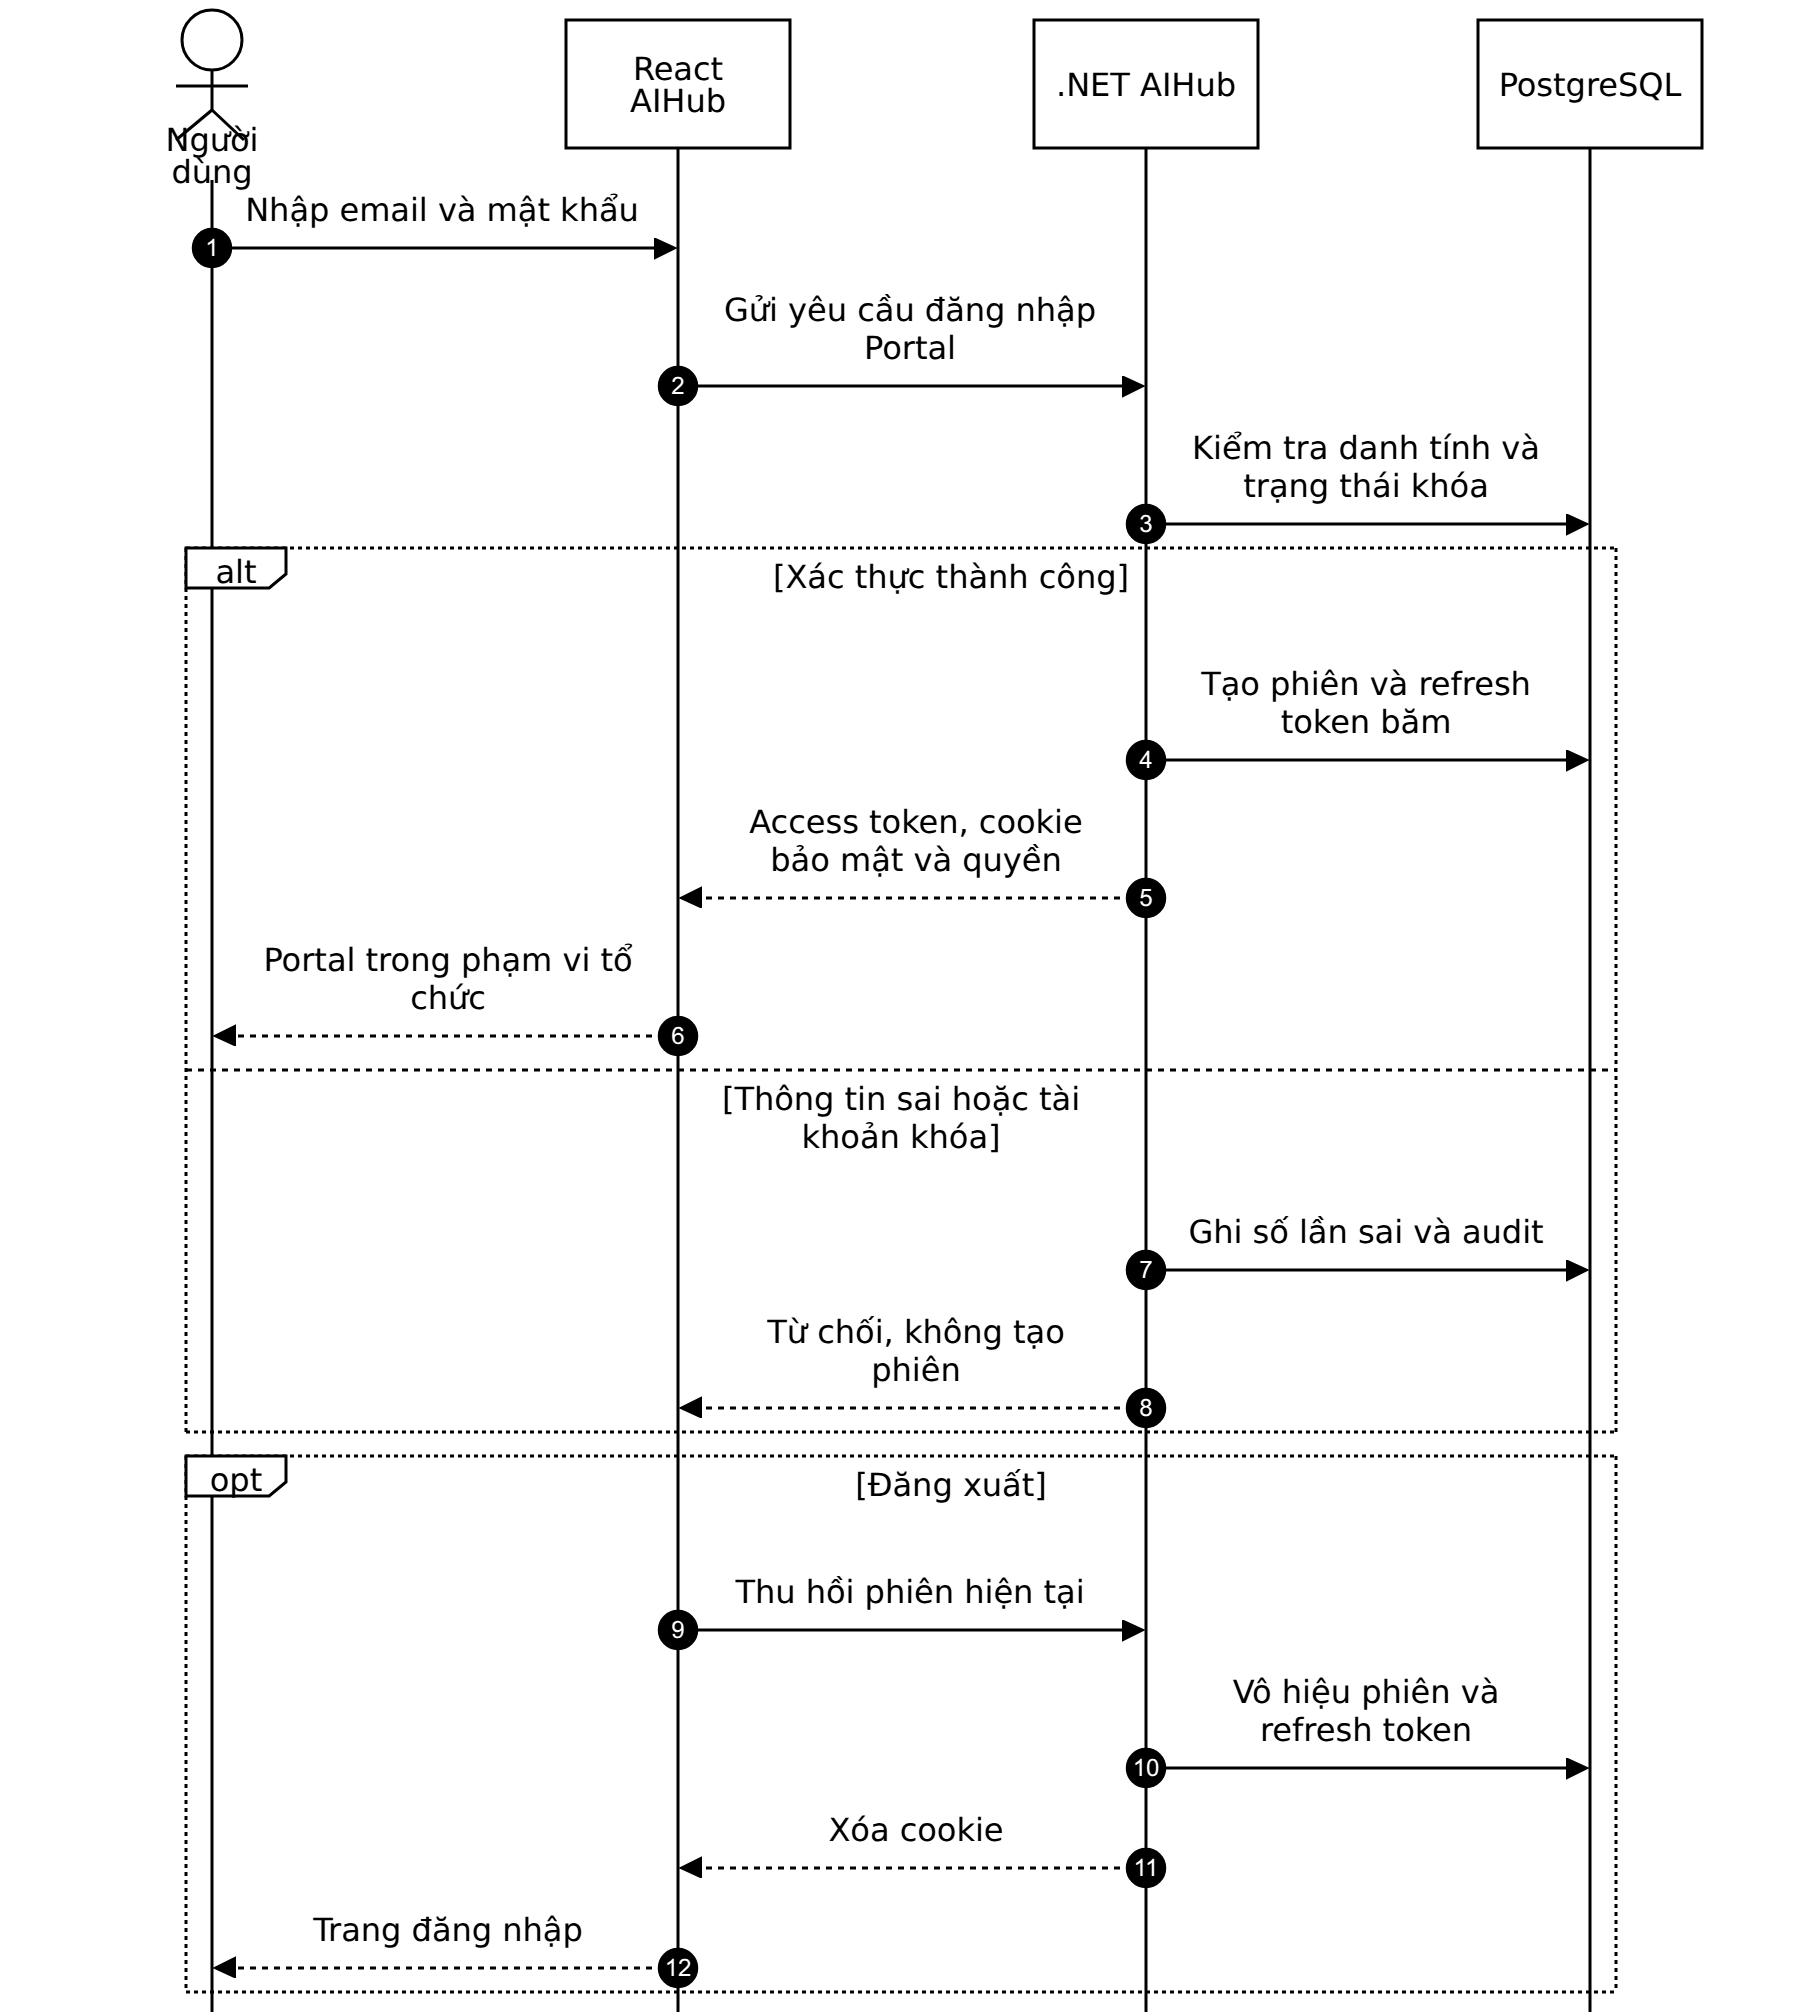
\includegraphics[width=\linewidth,height=.77\textheight,keepaspectratio]{Images/Sequence/AIHub/sequence_uc01_portal_auth.png}
\caption{Sequence diagram AIHub UC01 — Xác thực Developer Portal}
\label{sequence:aihub:sequence_uc01_portal_auth}
\end{figure}

Portal dùng danh tính người dùng; xác thực API đối tác là cơ chế riêng bằng credentials tổ chức.

\clearpage
\paragraph*{UC02. Quản lý khóa API}

\begin{figure}[H]
\centering
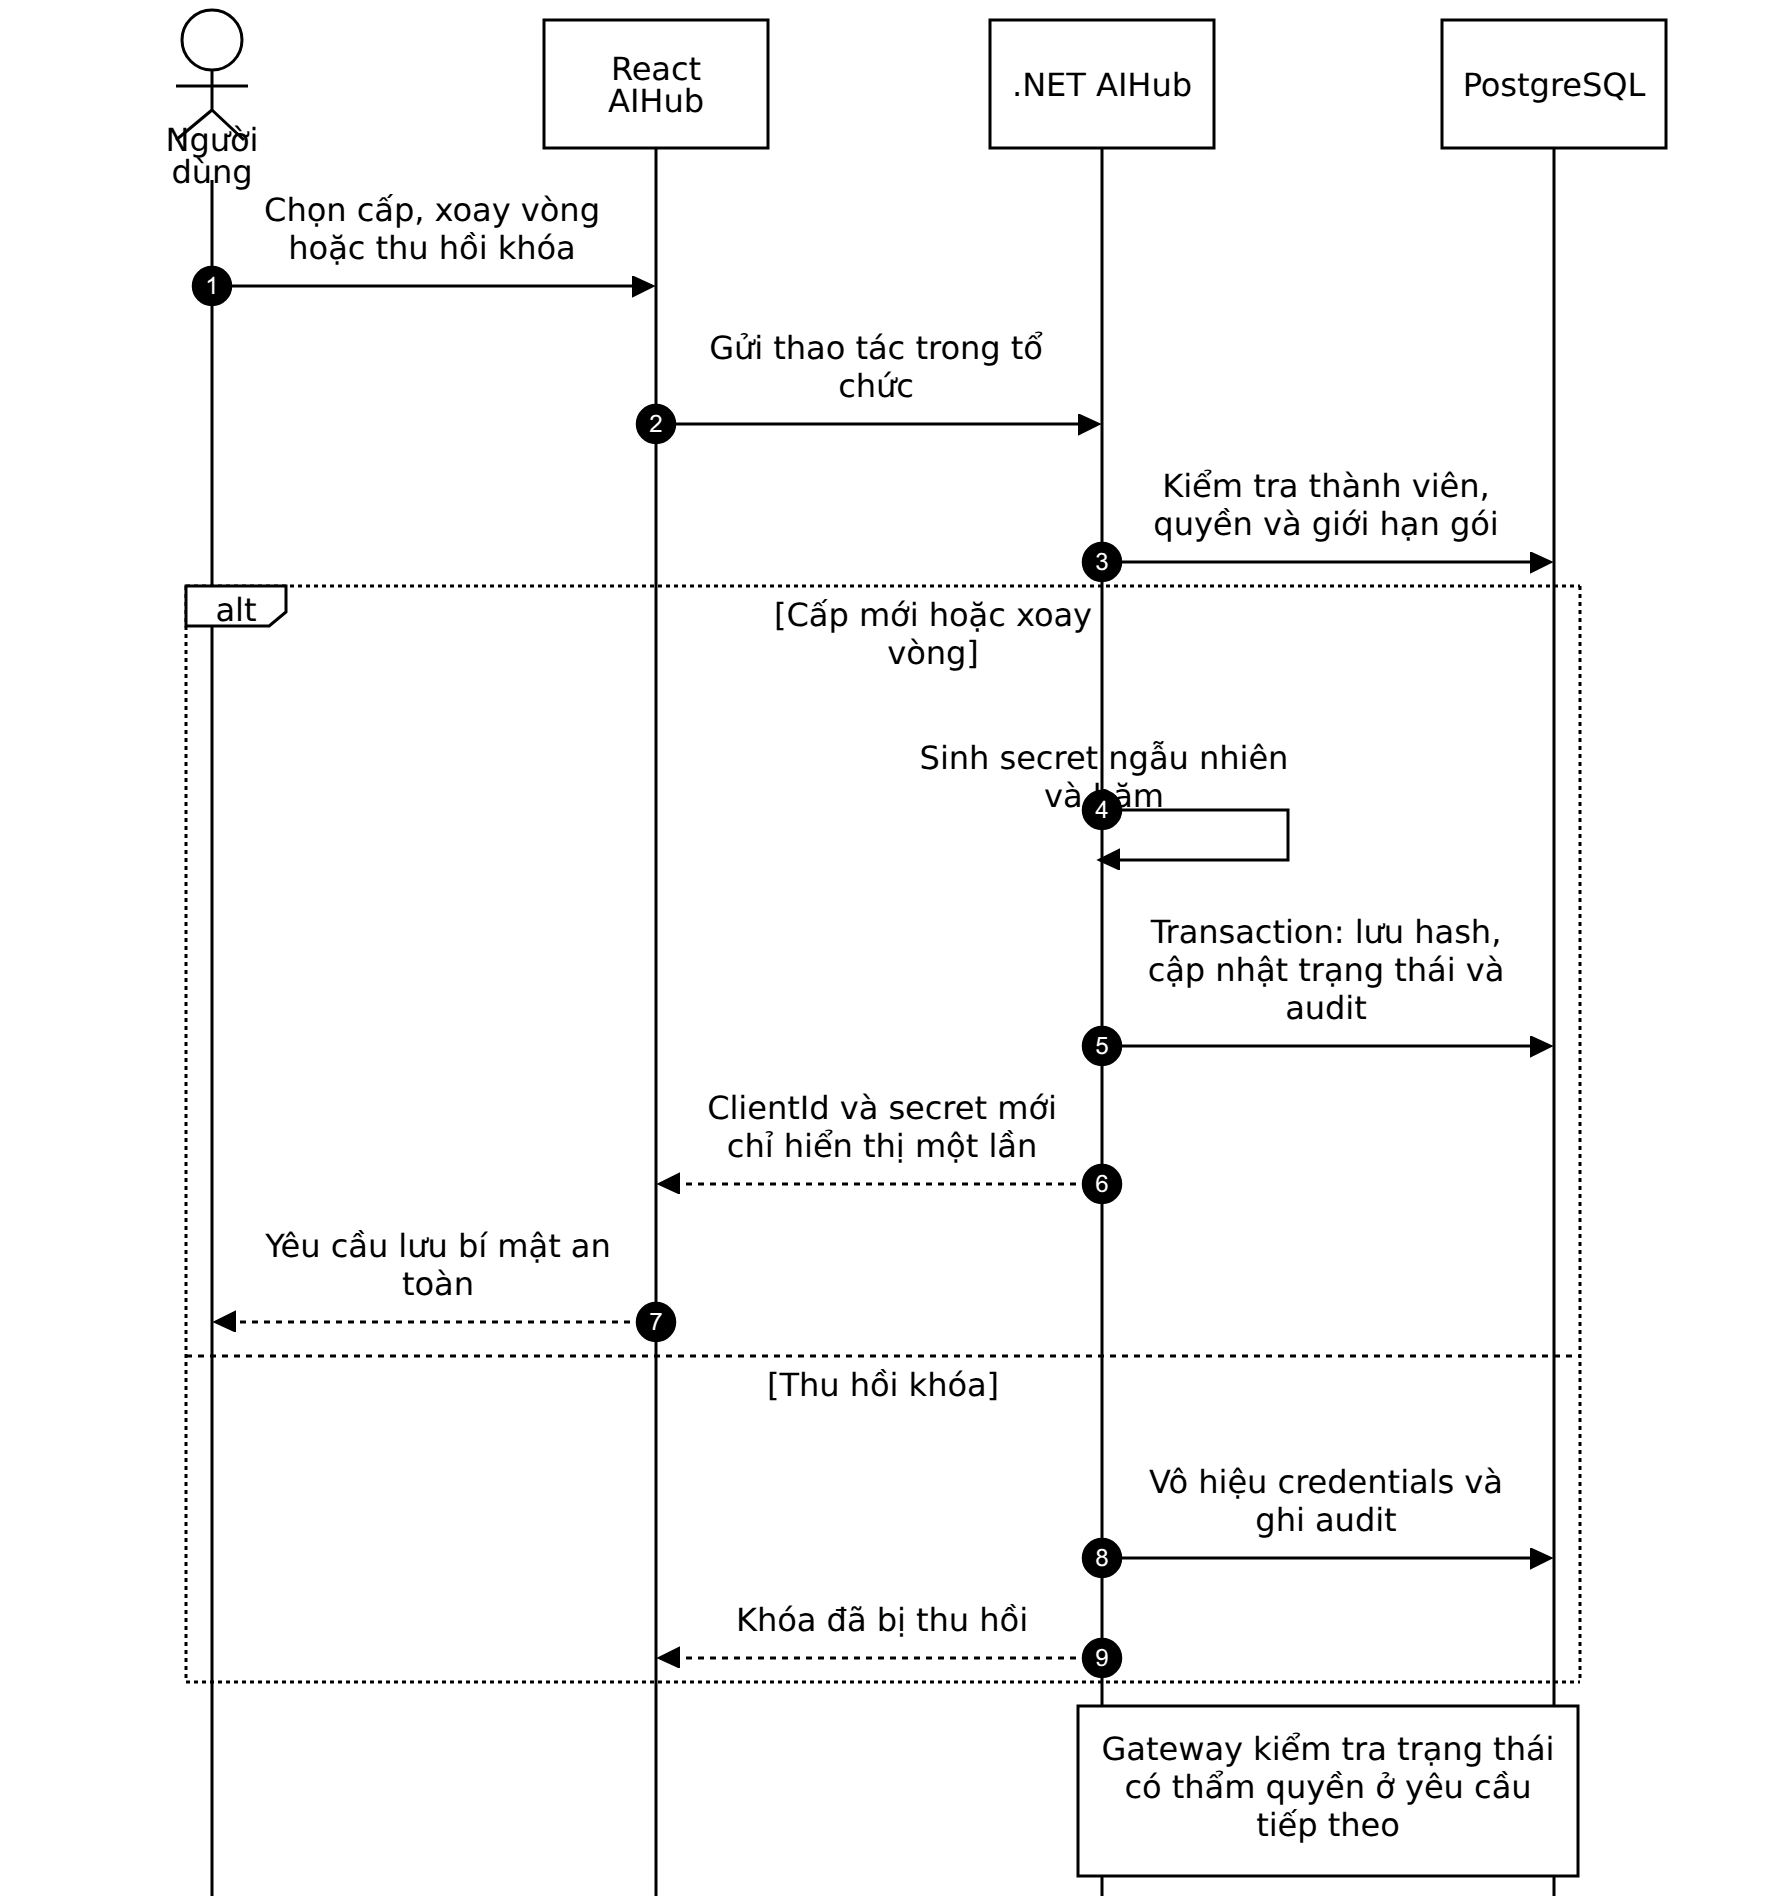
\includegraphics[width=\linewidth,height=.77\textheight,keepaspectratio]{Images/Sequence/AIHub/sequence_uc02_api_credentials.png}
\caption{Sequence diagram AIHub UC02 — Quản lý khóa API}
\label{sequence:aihub:sequence_uc02_api_credentials}
\end{figure}

Secret chỉ được trả một lần; phía máy chủ lưu hash và bảo đảm thu hồi có hiệu lực tại Gateway.

\clearpage
\paragraph*{UC03. Kiểm thử cURL Sandbox}

\begin{figure}[H]
\centering
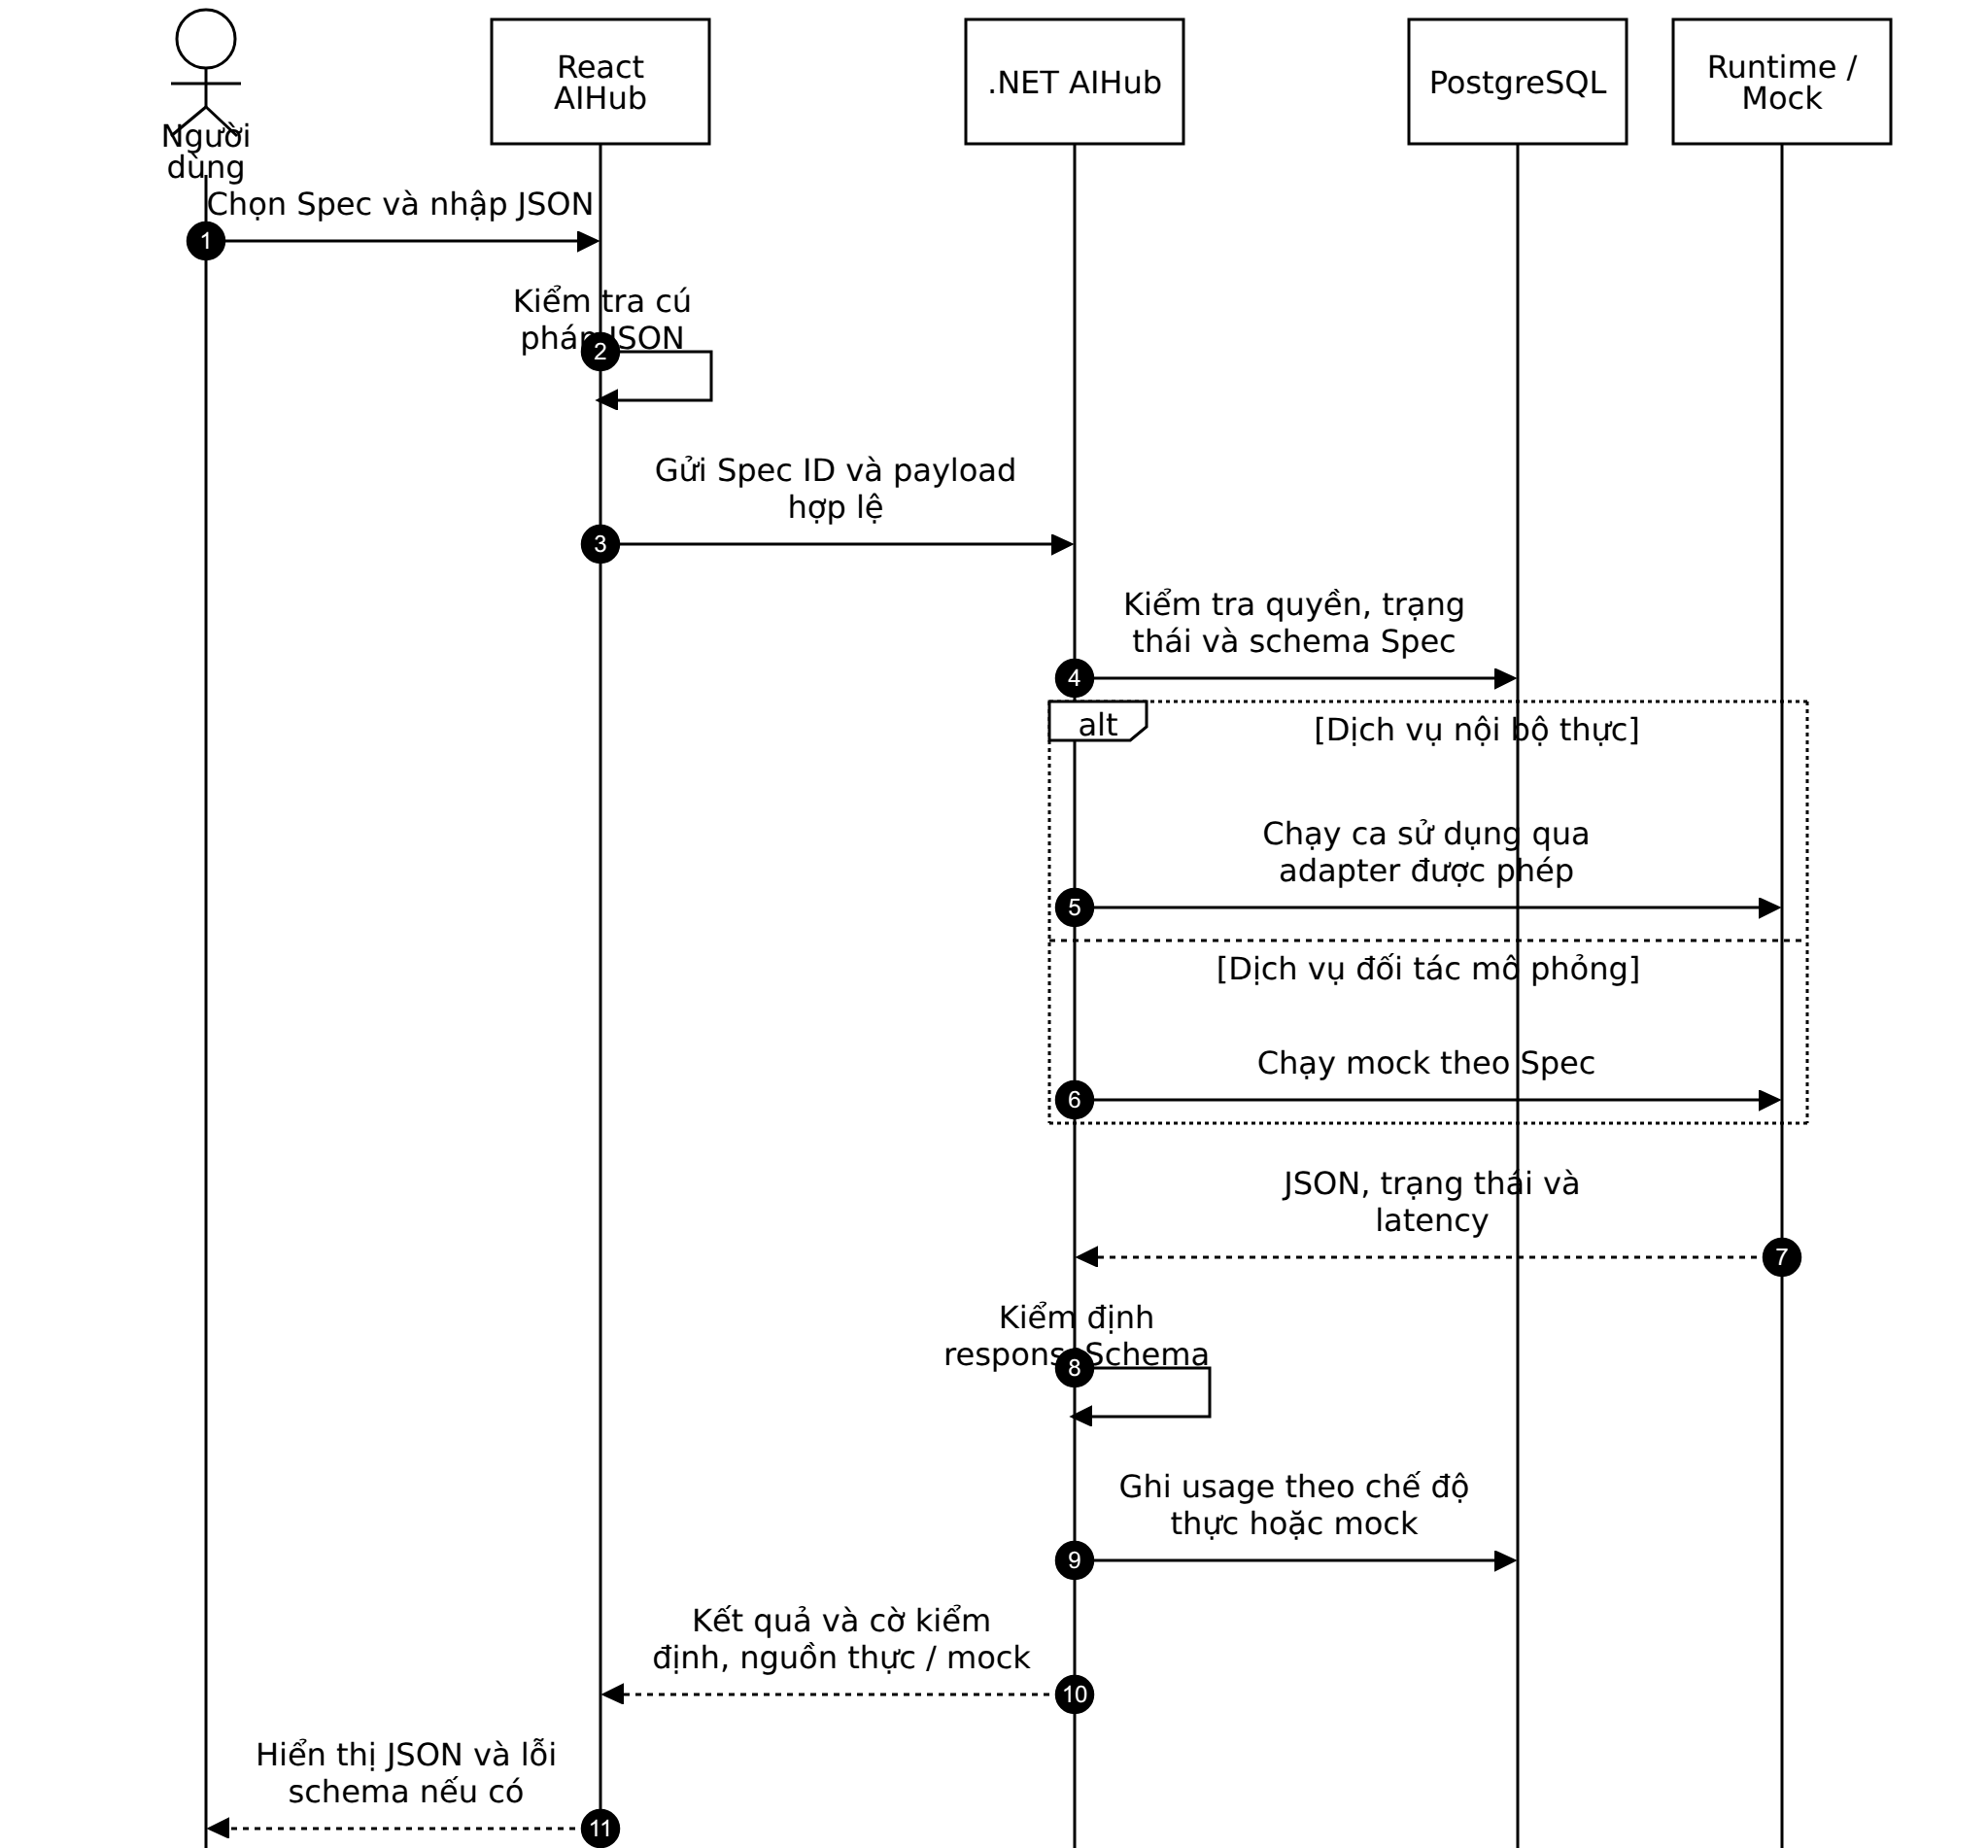
\includegraphics[width=\linewidth,height=.77\textheight,keepaspectratio]{Images/Sequence/AIHub/sequence_uc03_curl_sandbox.png}
\caption{Sequence diagram AIHub UC03 — Kiểm thử cURL Sandbox}
\label{sequence:aihub:sequence_uc03_curl_sandbox}
\end{figure}

Sandbox phân biệt chạy thật với mô phỏng và kiểm định đầu ra theo phiên bản Spec đang hoạt động.

\clearpage
\paragraph*{UC04. Gọi API sinh bài tập vi mô}

\begin{figure}[H]
\centering
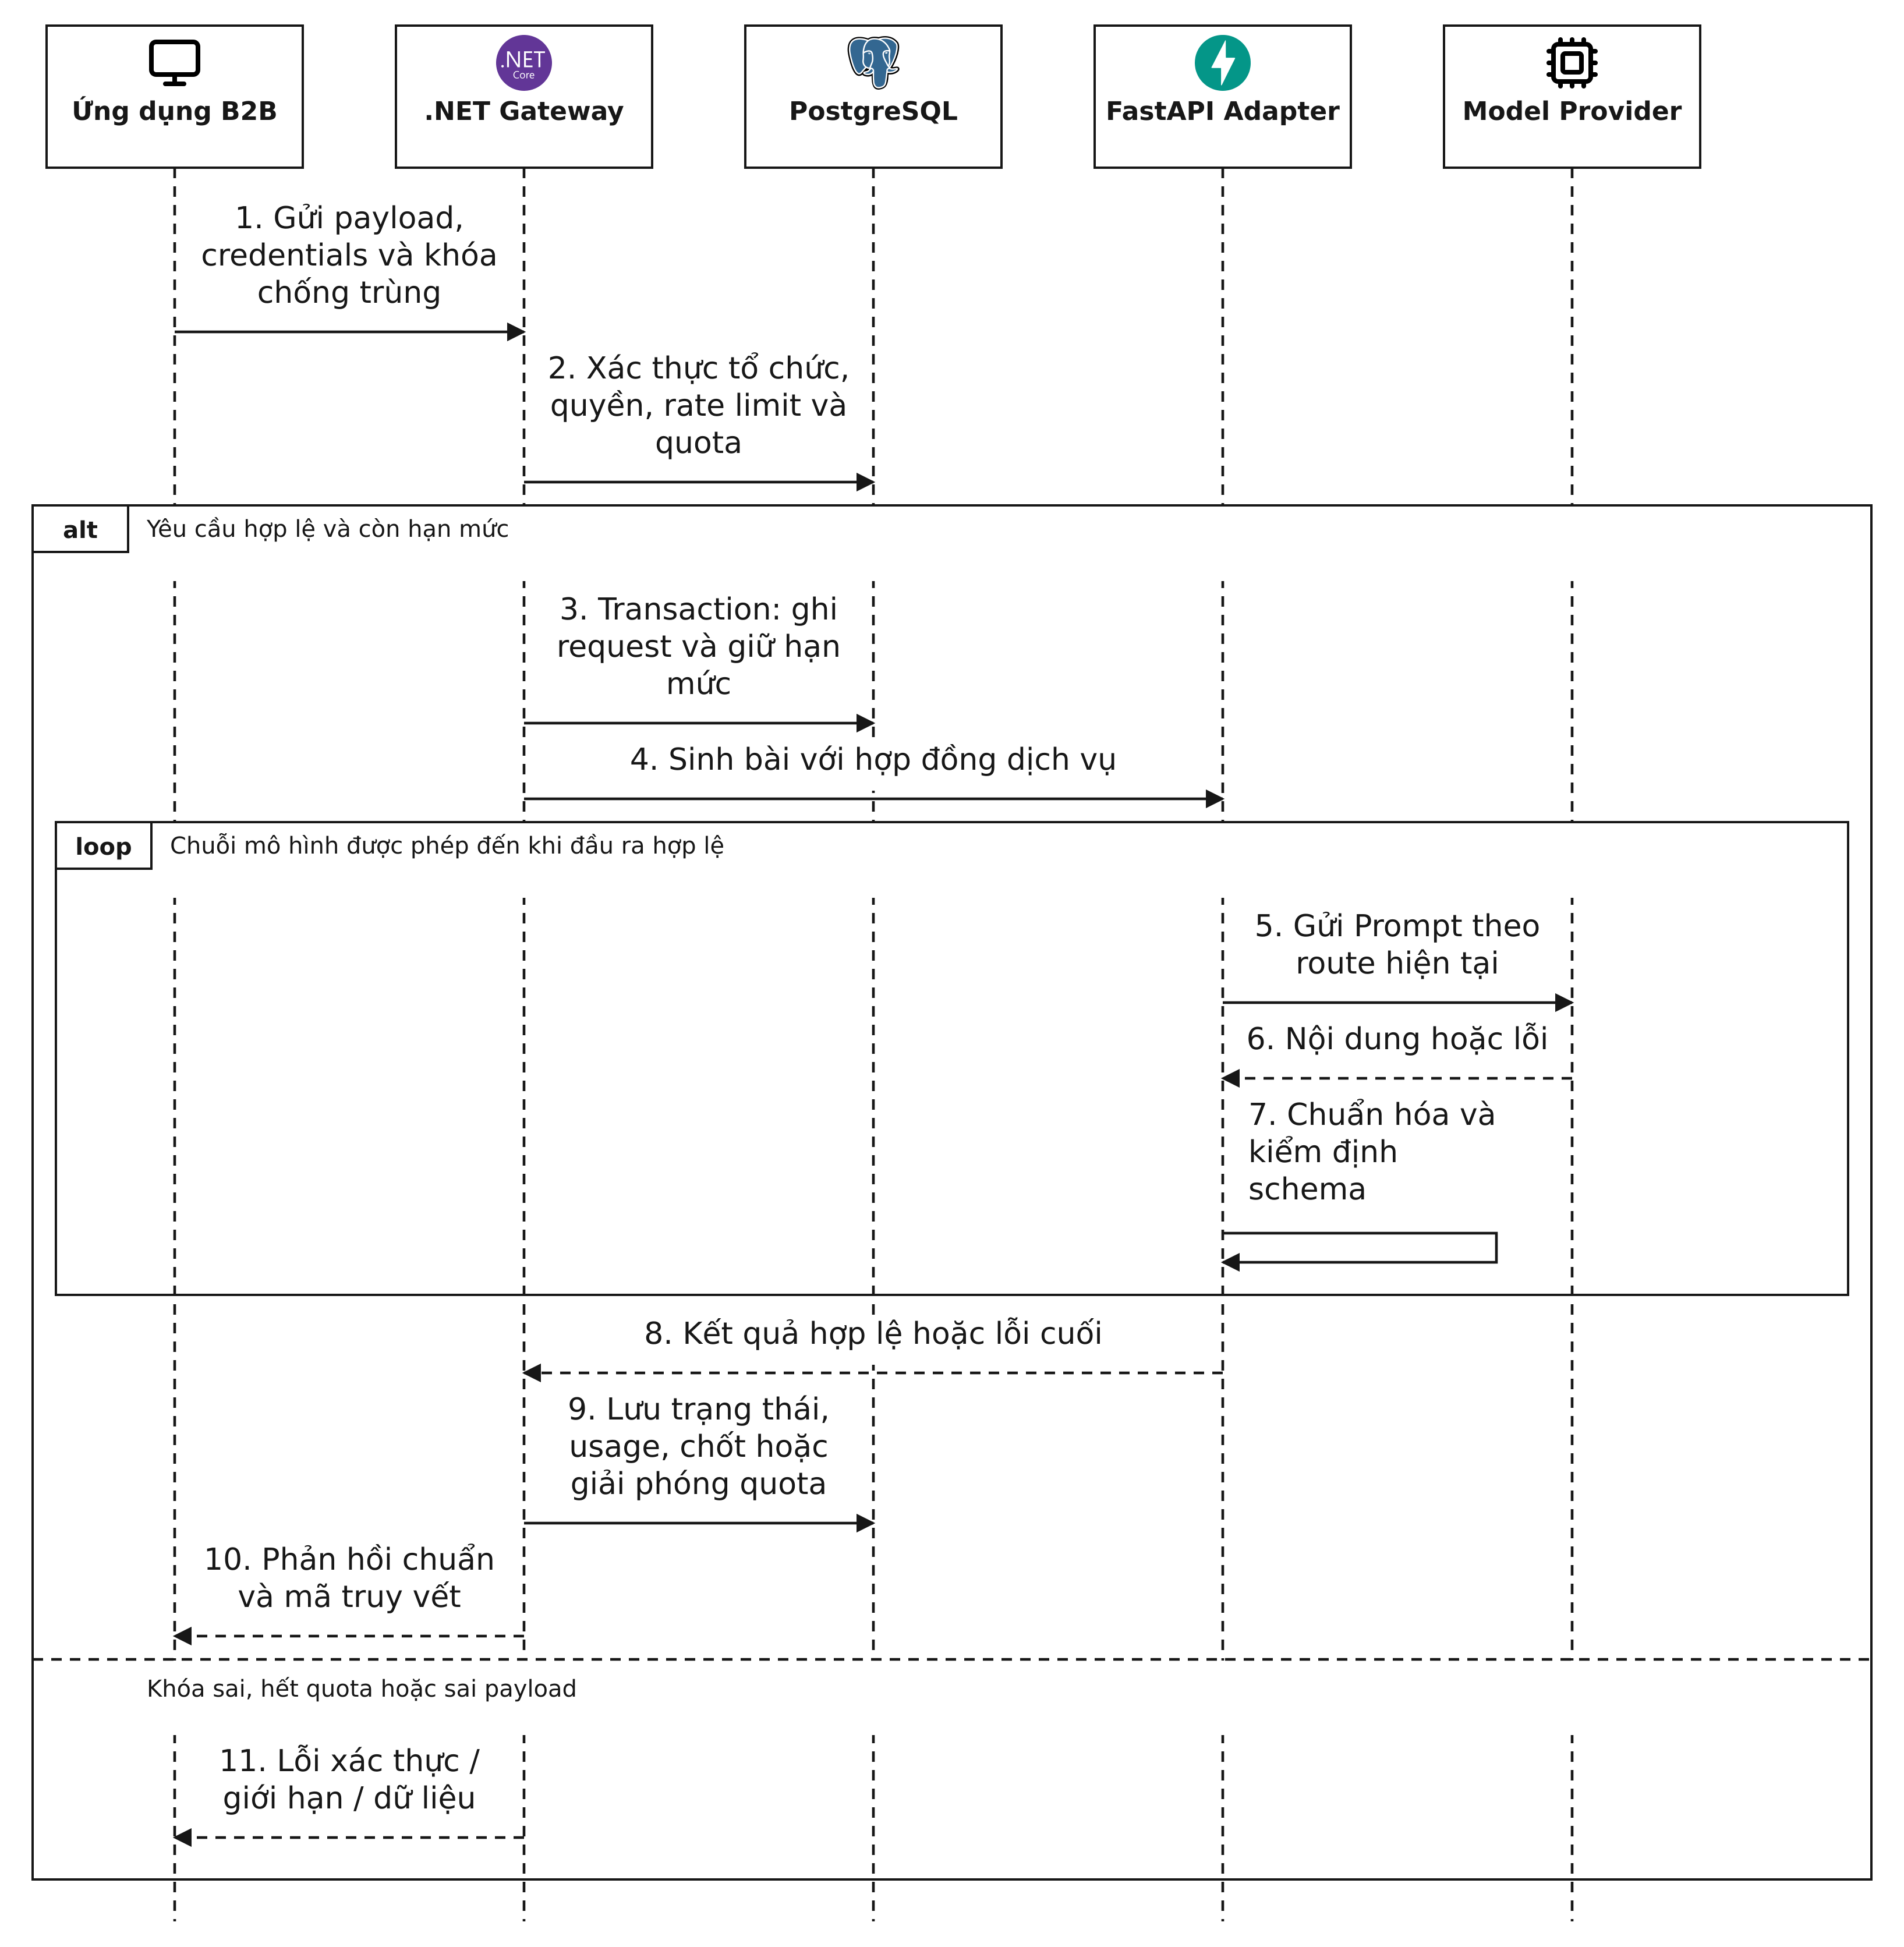
\includegraphics[width=\linewidth,height=.77\textheight,keepaspectratio]{Images/Sequence/AIHub/sequence_uc04_create_micro_exercise.png}
\caption{Sequence diagram AIHub UC04 — Gọi API sinh bài tập vi mô}
\label{sequence:aihub:sequence_uc04_create_micro_exercise}
\end{figure}

Gateway quản lý quyền và hạn mức B2B; adapter xử lý fallback rồi trả kết quả đã được kiểm định.

\clearpage
\paragraph*{UC05. Tra cứu hạn mức và nhật ký}

\begin{figure}[H]
\centering
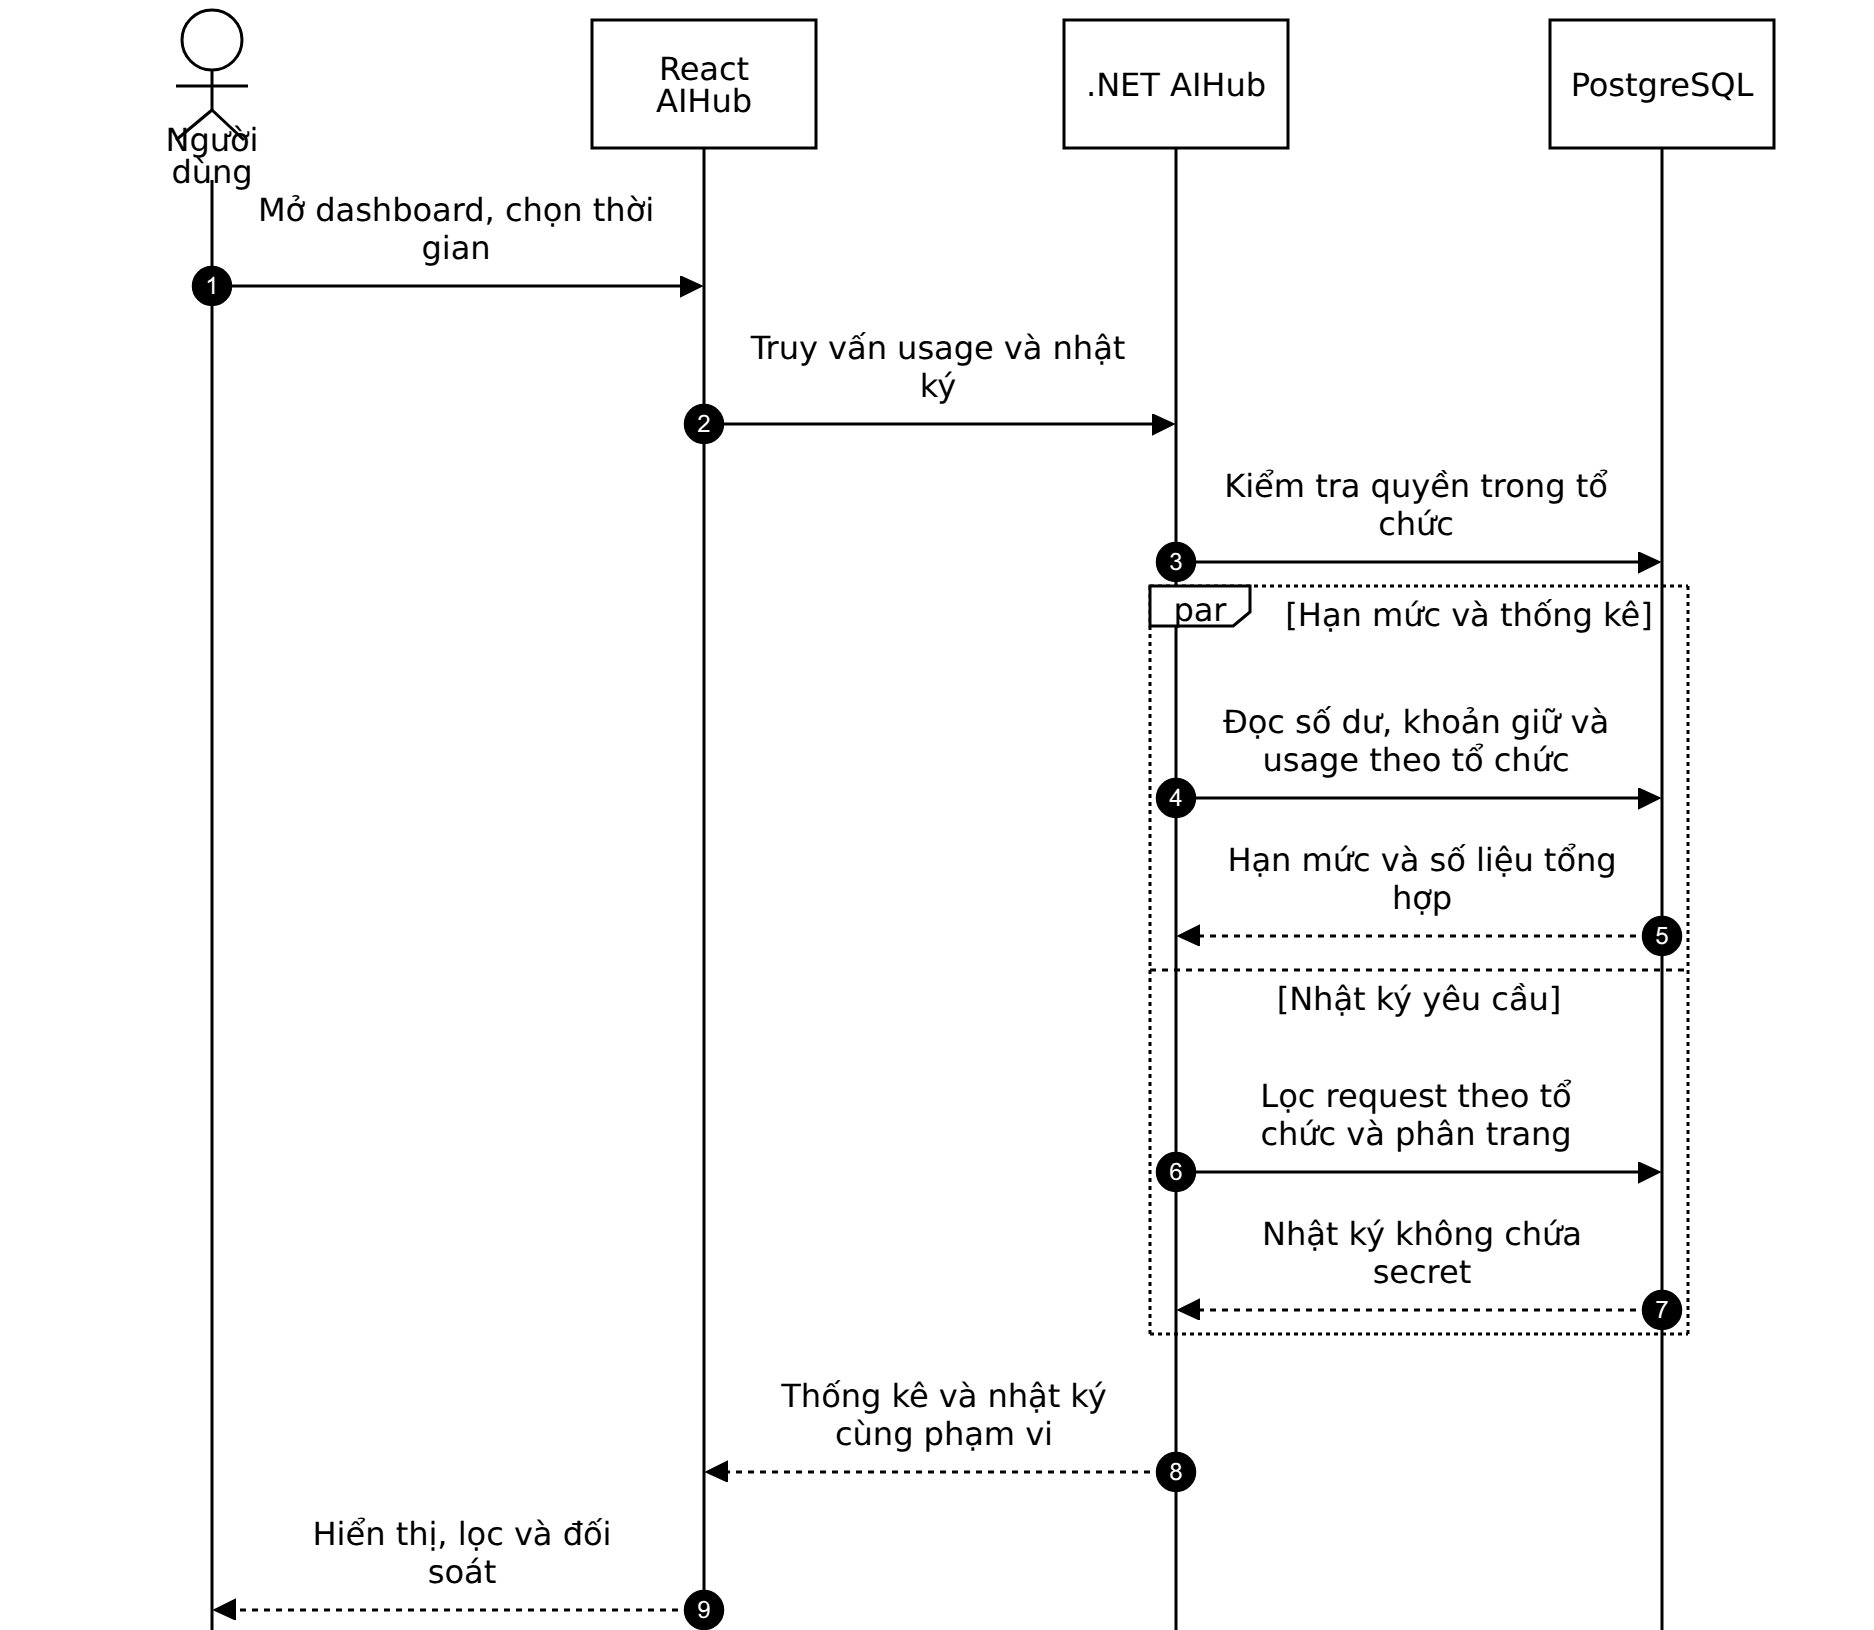
\includegraphics[width=\linewidth,height=.77\textheight,keepaspectratio]{Images/Sequence/AIHub/sequence_uc05_quota_usage_logs.png}
\caption{Sequence diagram AIHub UC05 — Tra cứu hạn mức và nhật ký}
\label{sequence:aihub:sequence_uc05_quota_usage_logs}
\end{figure}

Cả thống kê lẫn nhật ký được giới hạn theo tổ chức; các chi phí mô hình được tách khỏi hạn mức nghiệp vụ.

\clearpage
\paragraph*{UC06. Tra cứu dẫn chứng học thuật}

\begin{figure}[H]
\centering
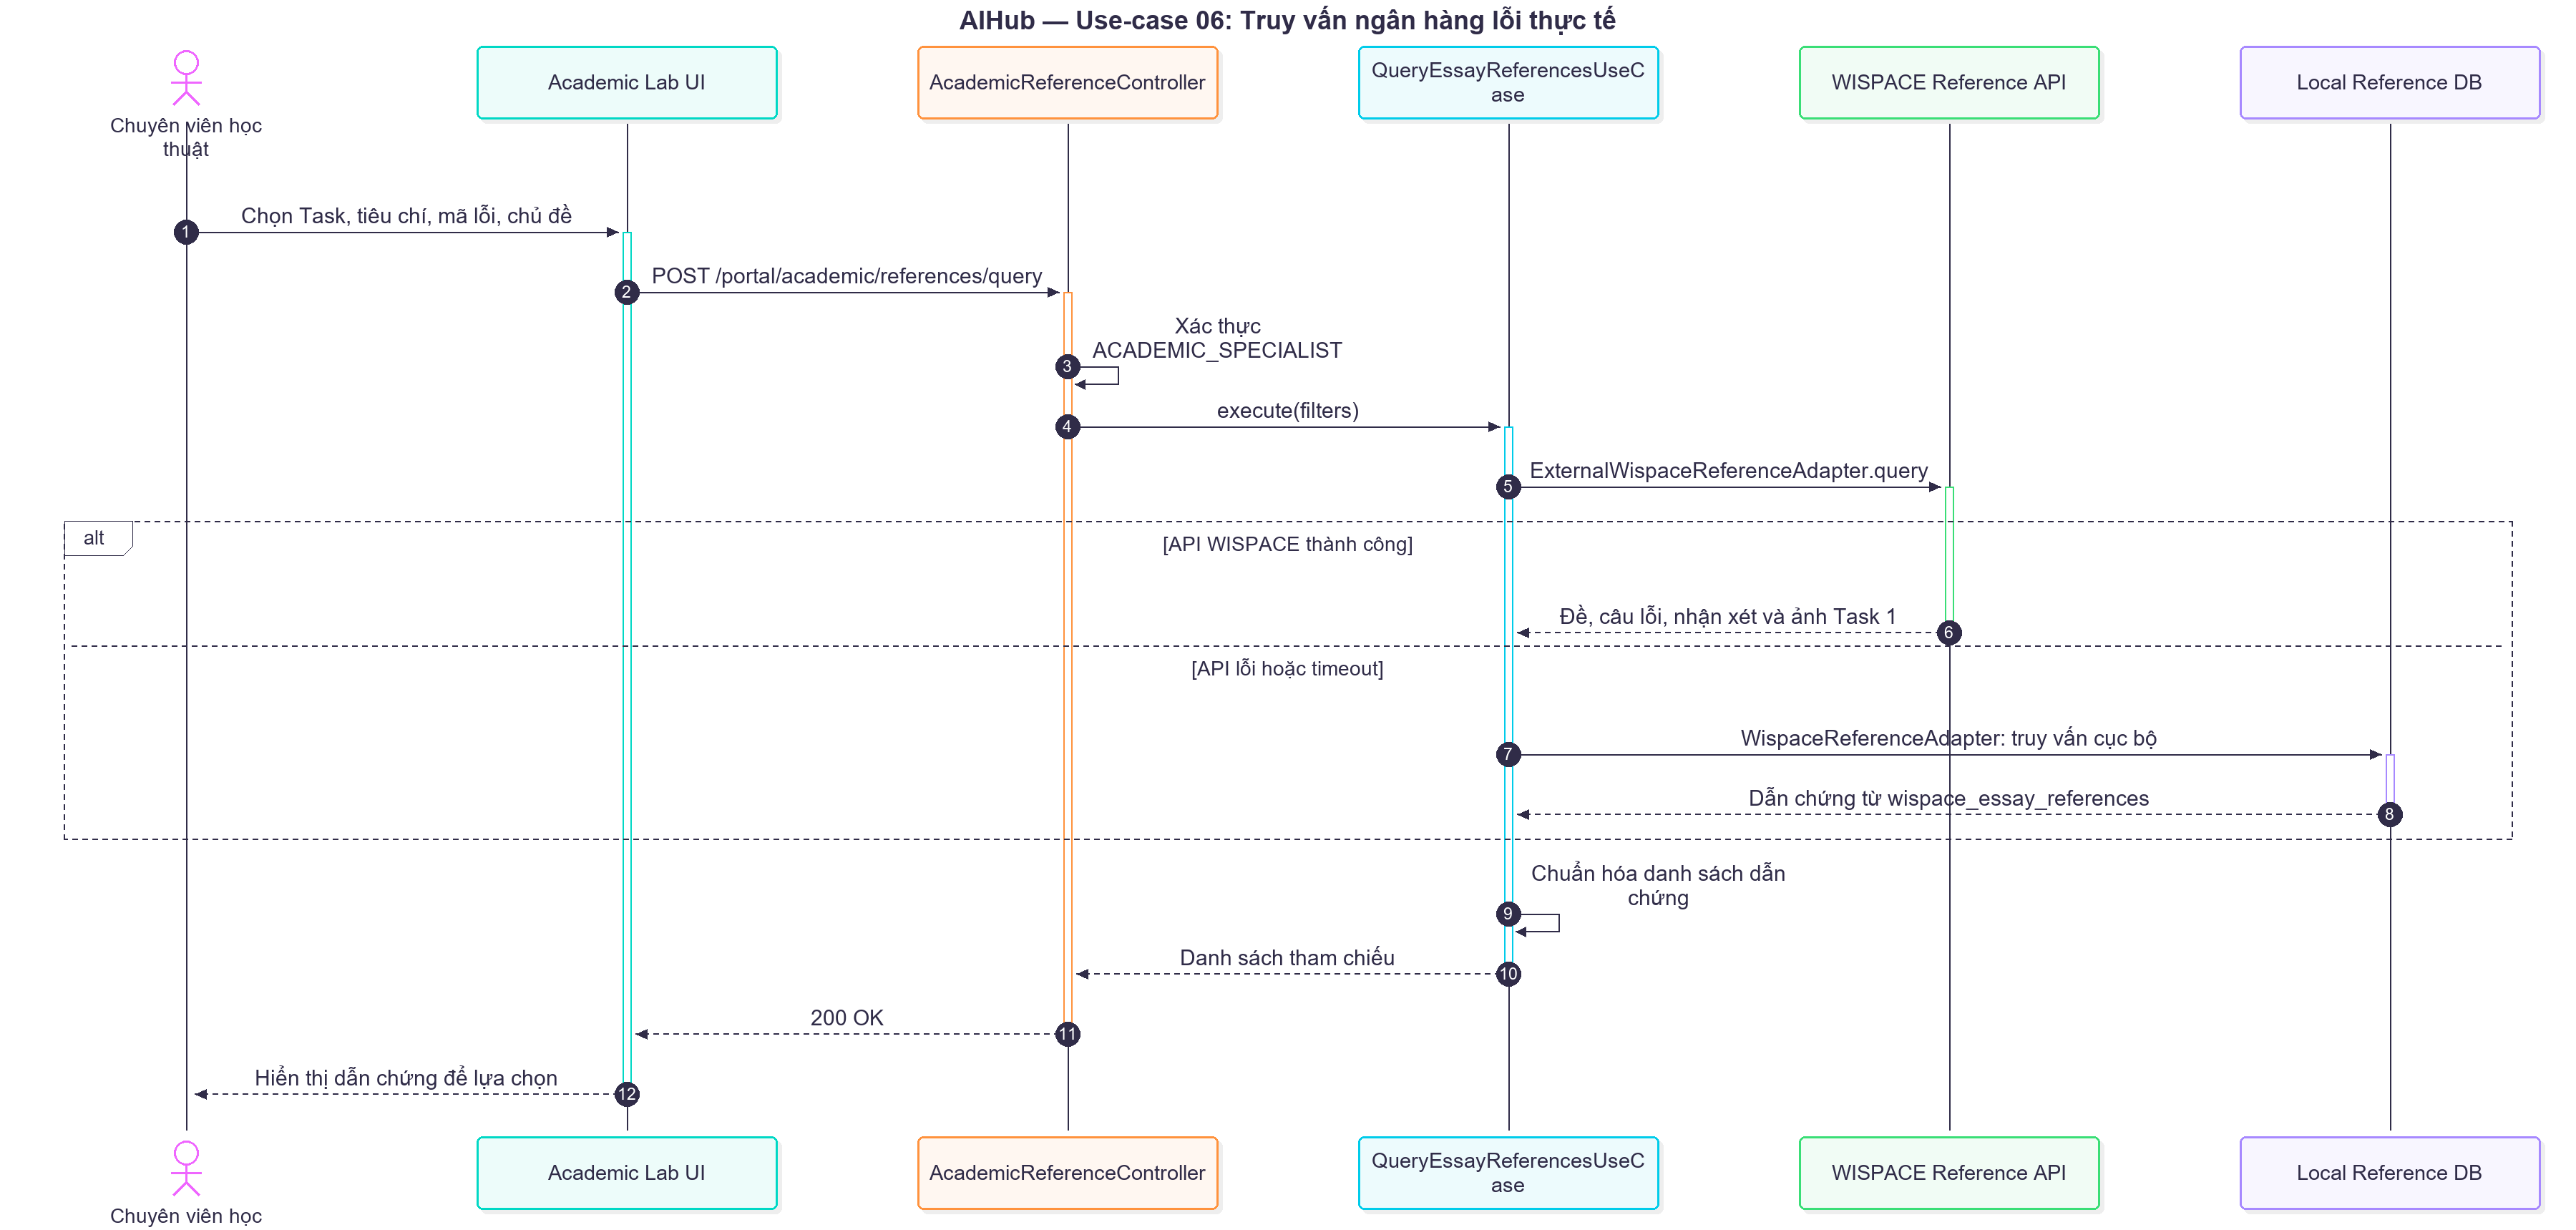
\includegraphics[width=\linewidth,height=.77\textheight,keepaspectratio]{Images/Sequence/AIHub/sequence_uc06_essay_references.png}
\caption{Sequence diagram AIHub UC06 — Tra cứu dẫn chứng học thuật}
\label{sequence:aihub:sequence_uc06_essay_references}
\end{figure}

Lỗi kết nối mới kích hoạt nguồn cục bộ; kết quả rỗng vẫn là kết quả nghiệp vụ hợp lệ.

\clearpage
\paragraph*{UC07. Sinh mẫu học thuật}

\begin{figure}[H]
\centering
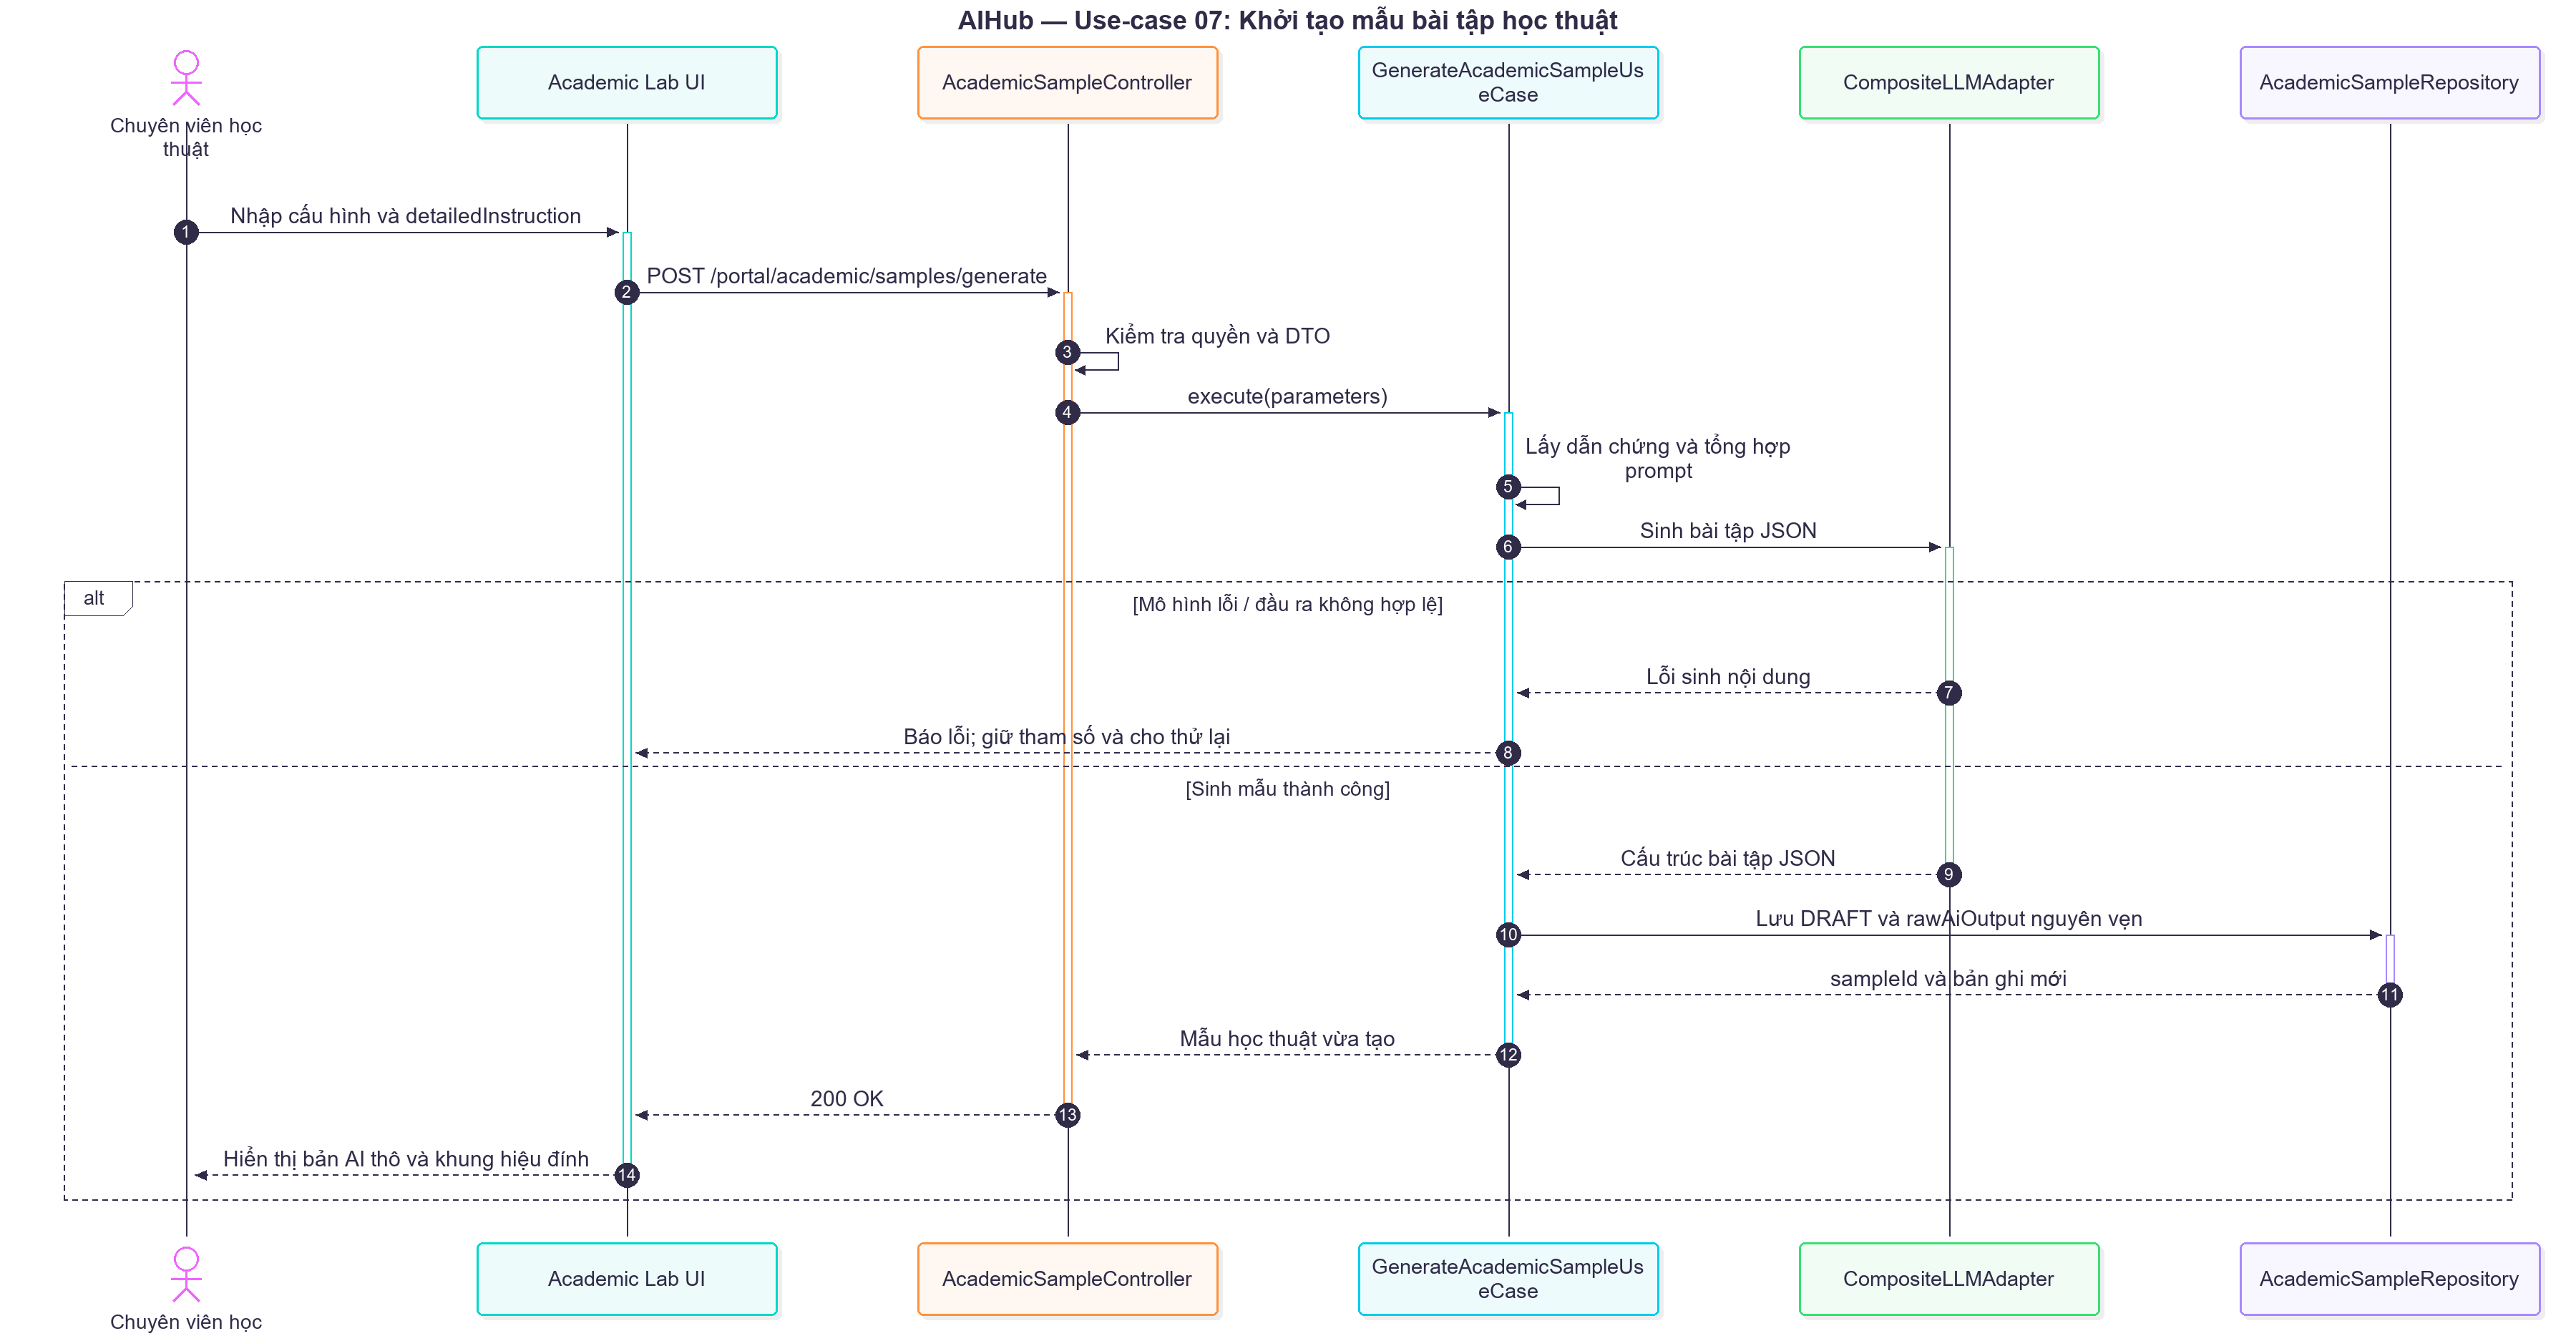
\includegraphics[width=\linewidth,height=.77\textheight,keepaspectratio]{Images/Sequence/AIHub/sequence_uc07_generate_academic_sample.png}
\caption{Sequence diagram AIHub UC07 — Sinh mẫu học thuật}
\label{sequence:aihub:sequence_uc07_generate_academic_sample}
\end{figure}

Chỉ tạo DRAFT khi đã có đầu ra hợp lệ; lưu Prompt và phiên bản mô hình để truy vết.

\clearpage
\paragraph*{UC08. Hiệu đính và chấm điểm mẫu}

\begin{figure}[H]
\centering
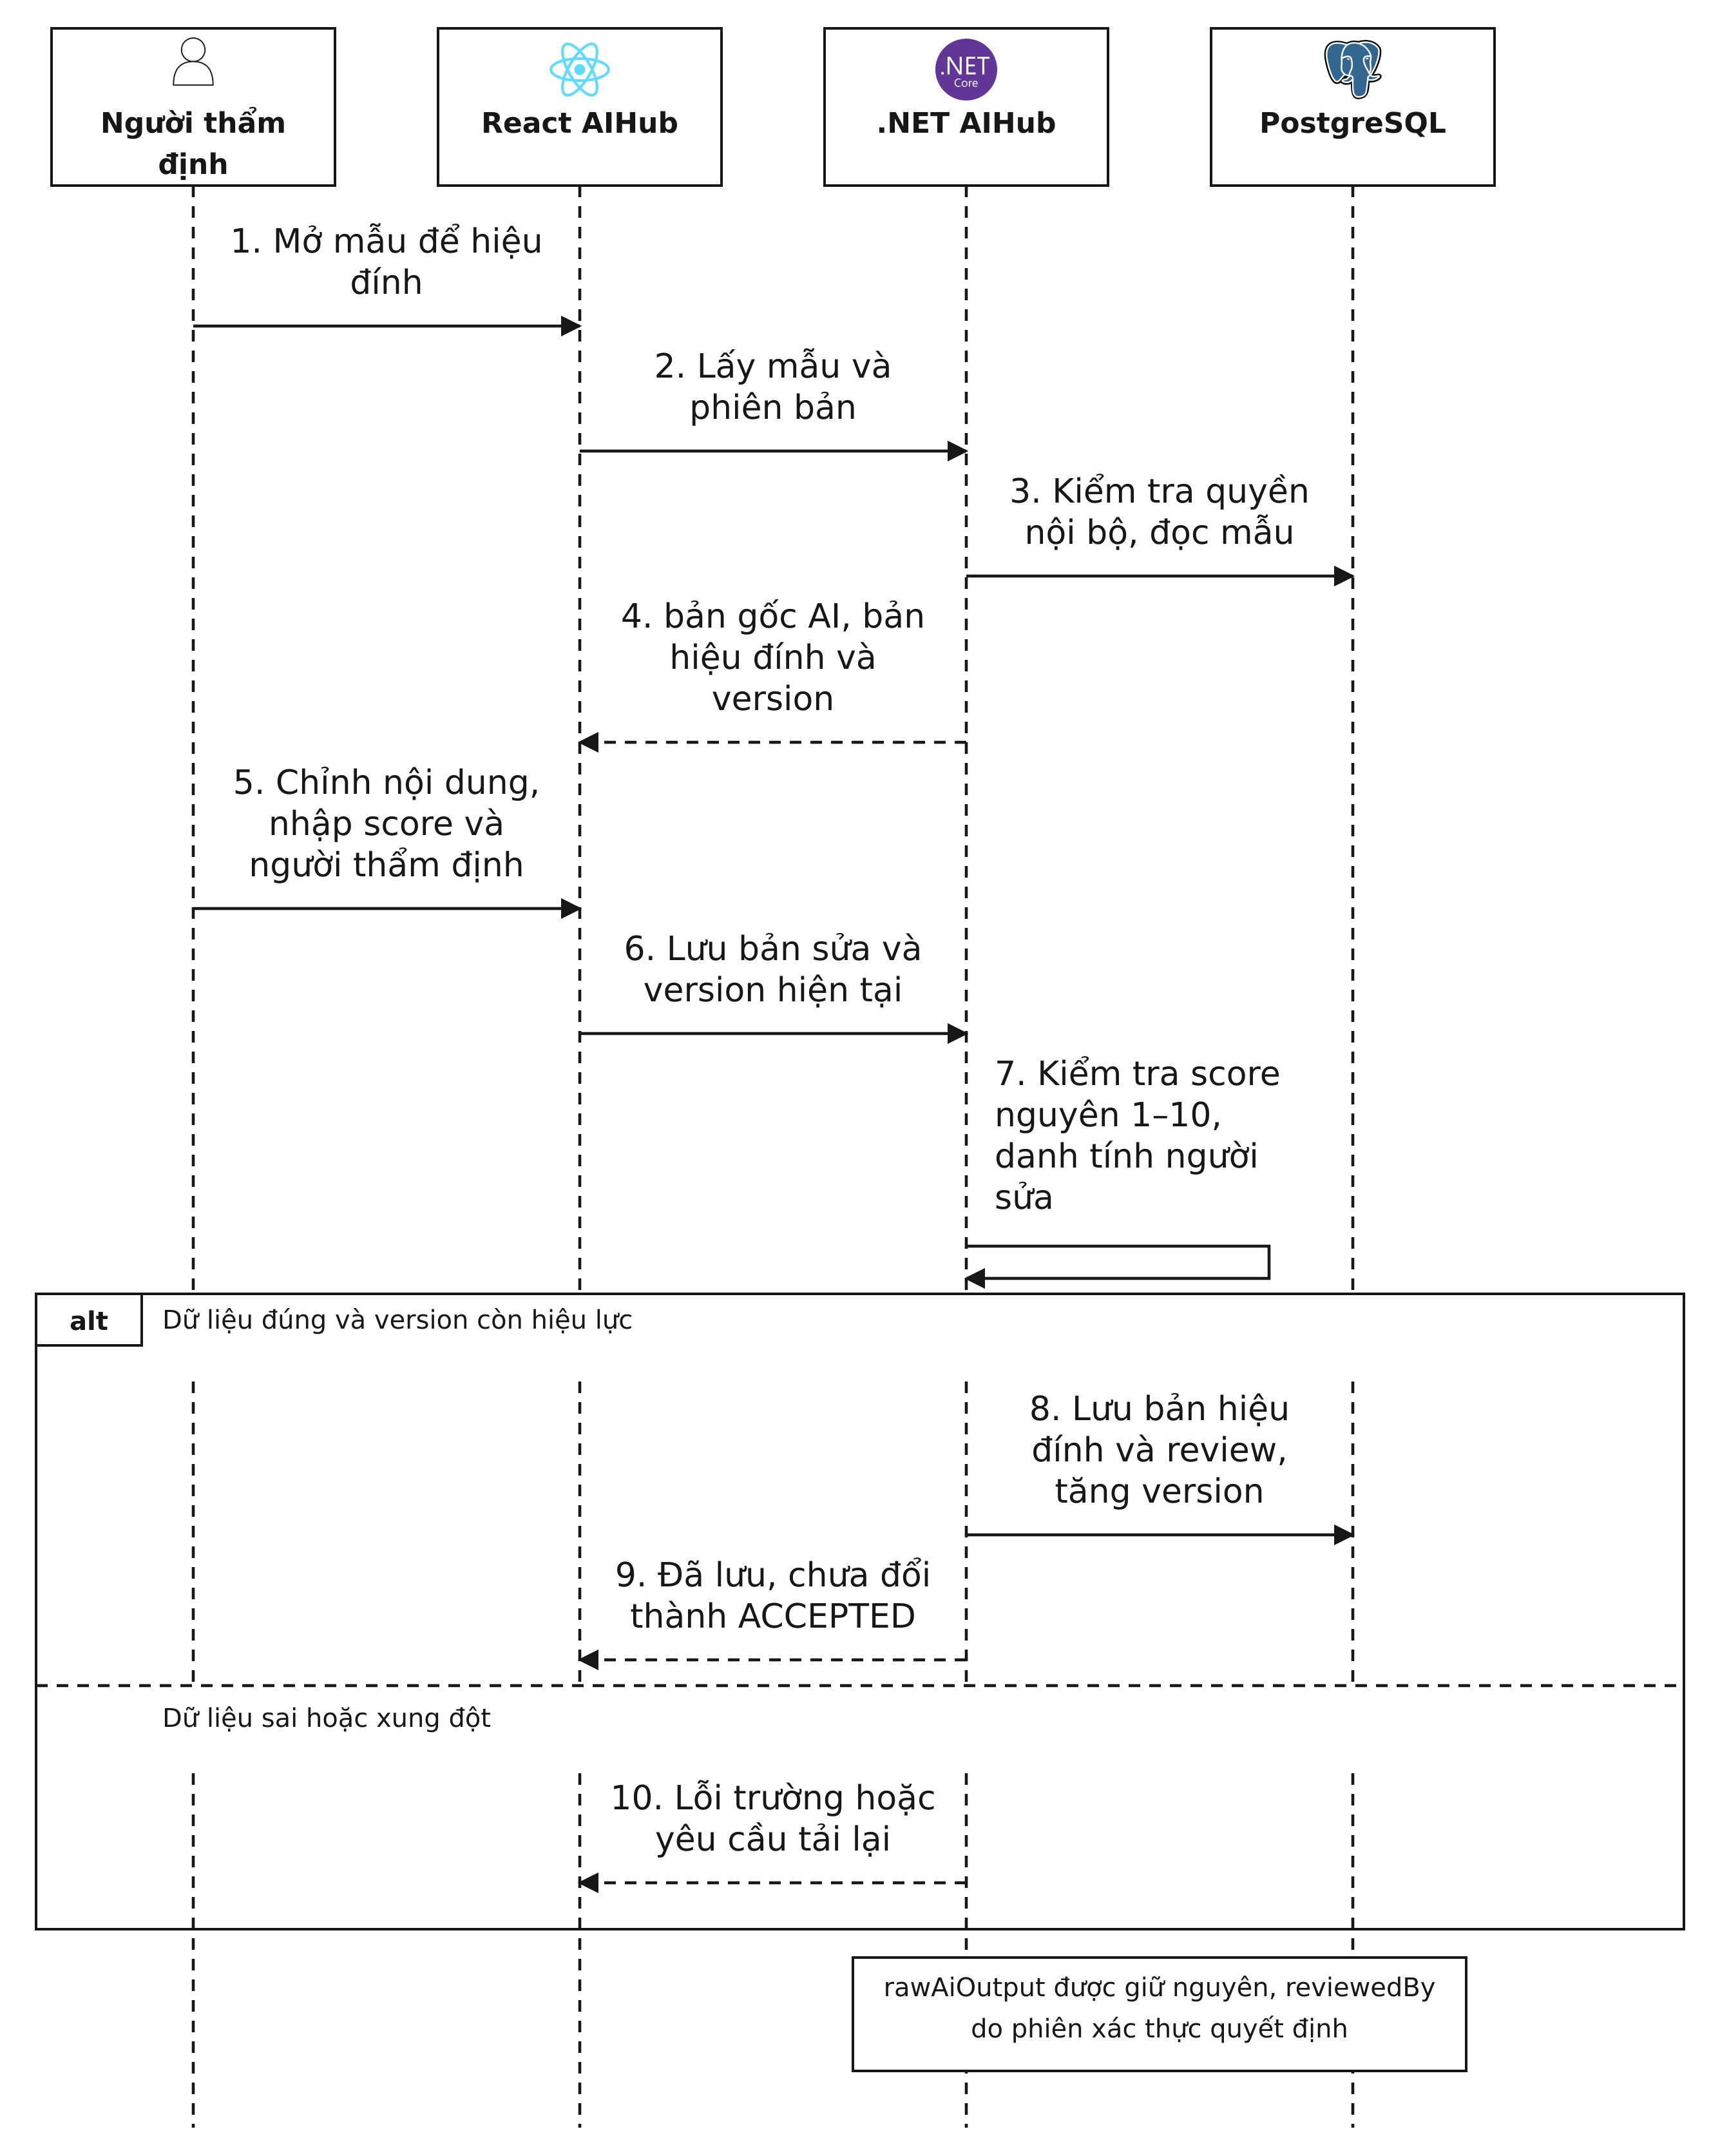
\includegraphics[width=\linewidth,height=.77\textheight,keepaspectratio]{Images/Sequence/AIHub/sequence_uc08_review_score_sample.png}
\caption{Sequence diagram AIHub UC08 — Hiệu đính và chấm điểm mẫu}
\label{sequence:aihub:sequence_uc08_review_score_sample}
\end{figure}

Lưu bản sửa không tự chấp thuận mẫu; kiểm tra phiên bản và danh tính người thẩm định trên máy chủ.

\clearpage
\paragraph*{UC09. Chấp thuận mẫu học thuật}

\begin{figure}[H]
\centering
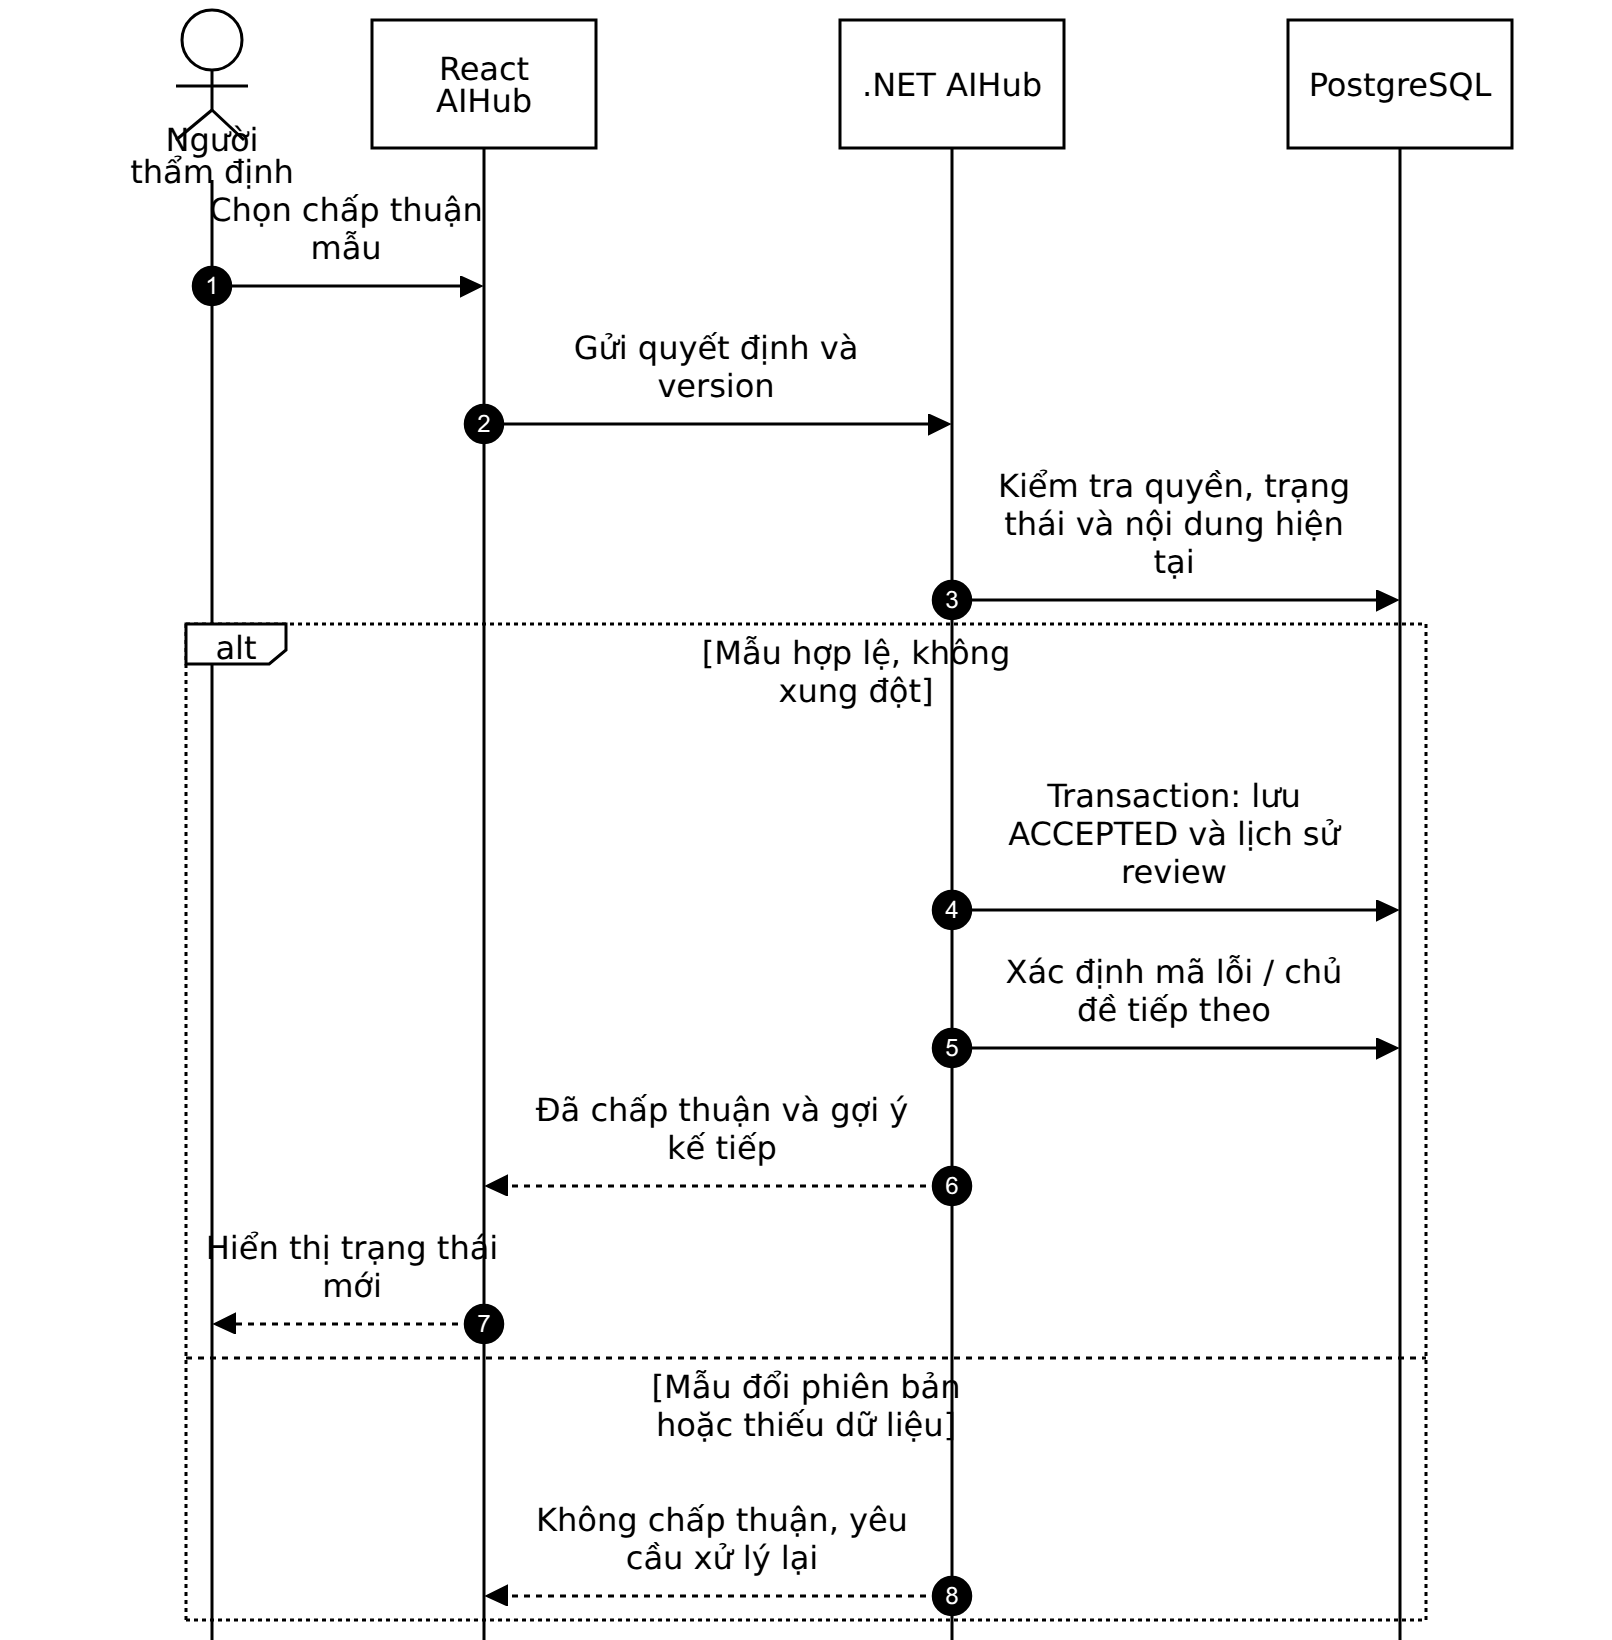
\includegraphics[width=\linewidth,height=.77\textheight,keepaspectratio]{Images/Sequence/AIHub/sequence_uc09_accept_sample.png}
\caption{Sequence diagram AIHub UC09 — Chấp thuận mẫu học thuật}
\label{sequence:aihub:sequence_uc09_accept_sample}
\end{figure}

Quyết định chấp thuận là giao dịch độc lập, có kiểm tra trạng thái và phiên bản trước khi xoay vòng lỗi.

\clearpage
\paragraph*{UC10. Từ chối mẫu học thuật}

\begin{figure}[H]
\centering
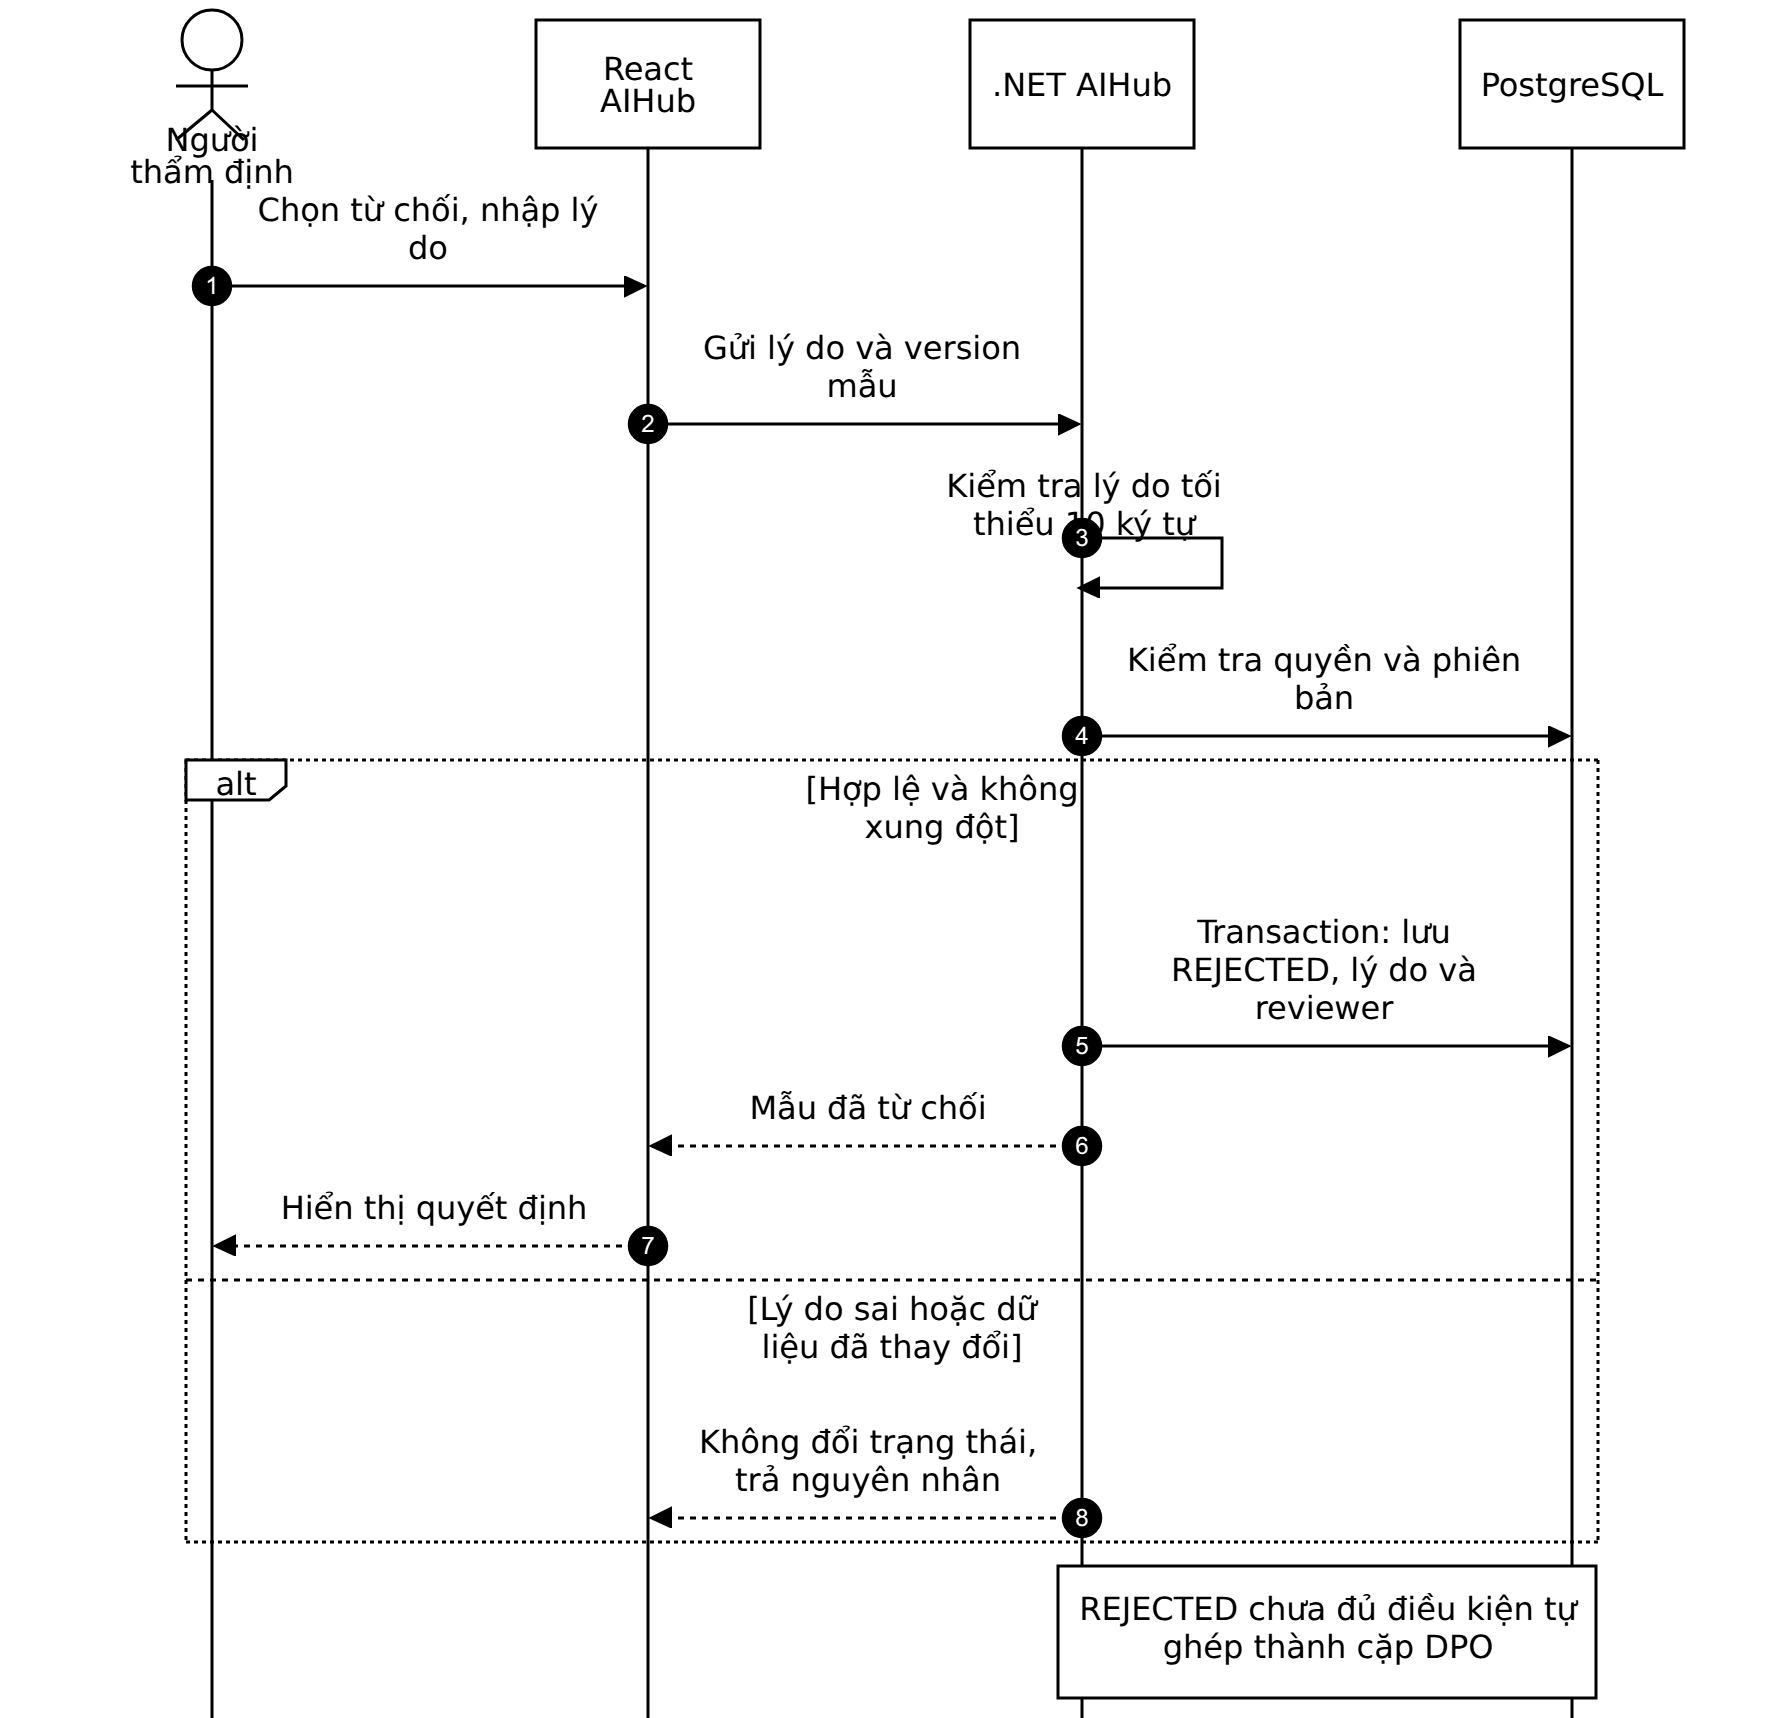
\includegraphics[width=\linewidth,height=.77\textheight,keepaspectratio]{Images/Sequence/AIHub/sequence_uc10_reject_sample.png}
\caption{Sequence diagram AIHub UC10 — Từ chối mẫu học thuật}
\label{sequence:aihub:sequence_uc10_reject_sample}
\end{figure}

Từ chối bảo toàn nội dung gốc và lý do; trạng thái REJECTED không tự biến mẫu thành dữ liệu DPO hợp lệ.

\clearpage
\paragraph*{UC11. Quản lý kho mẫu học thuật}

\begin{figure}[H]
\centering
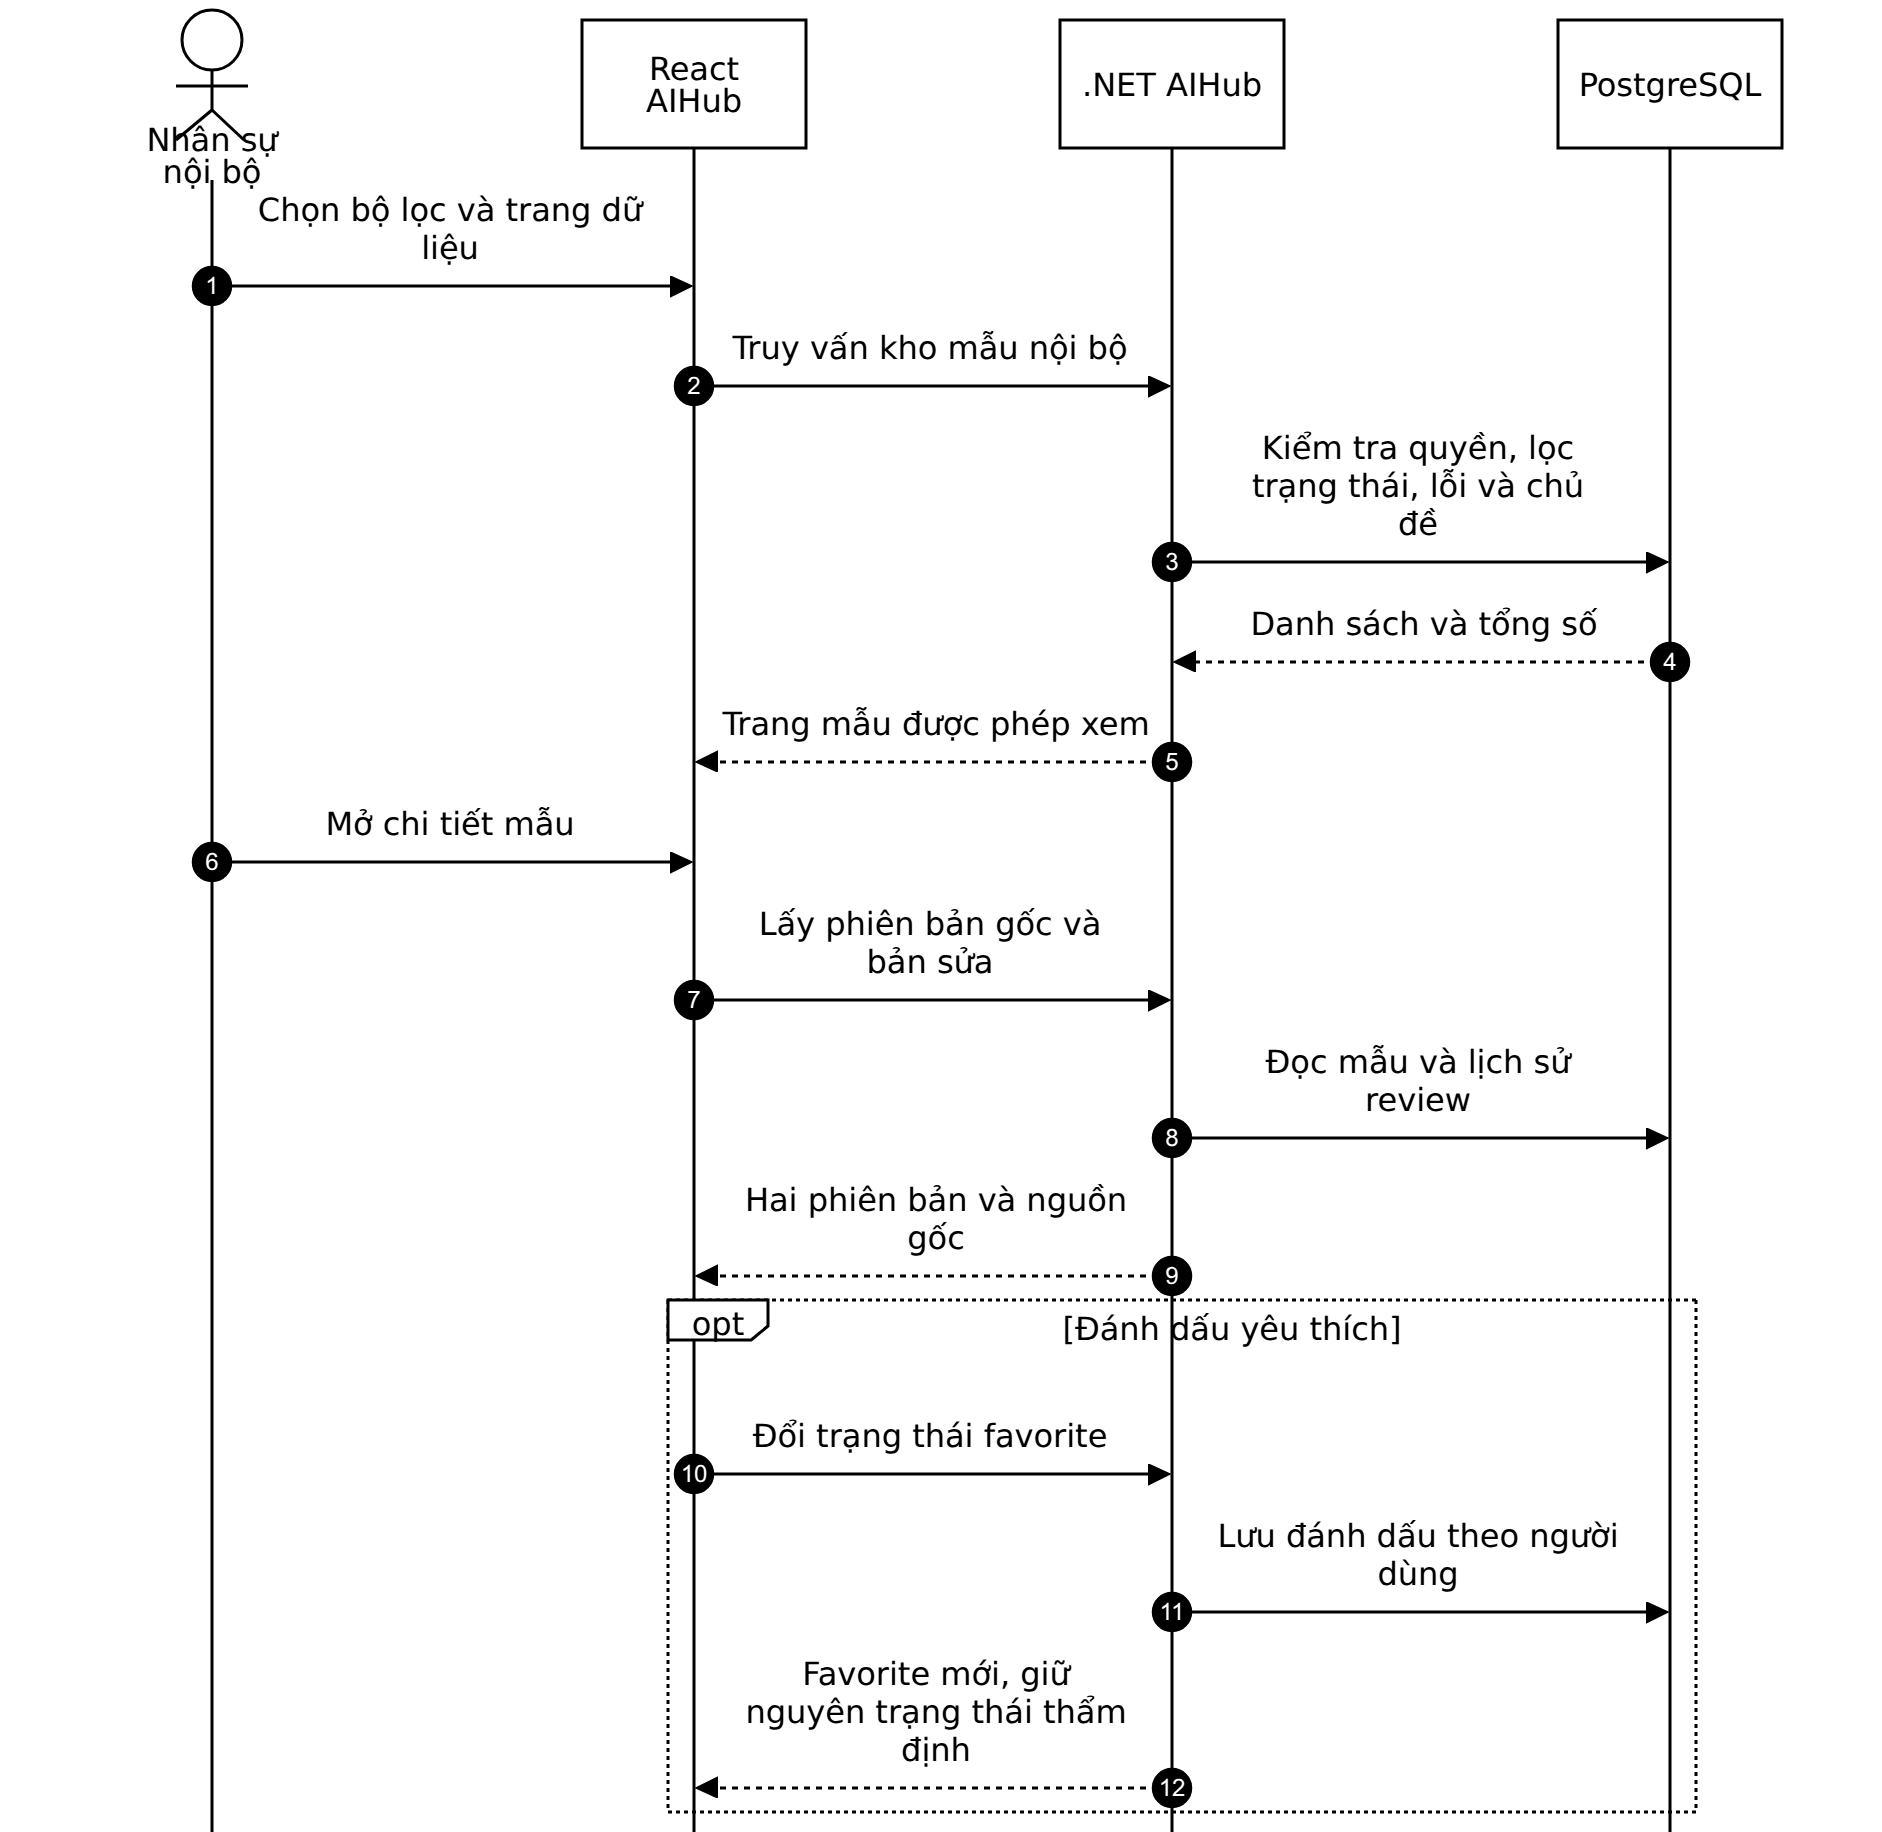
\includegraphics[width=\linewidth,height=.77\textheight,keepaspectratio]{Images/Sequence/AIHub/sequence_uc11_academic_inventory.png}
\caption{Sequence diagram AIHub UC11 — Quản lý kho mẫu học thuật}
\label{sequence:aihub:sequence_uc11_academic_inventory}
\end{figure}

Kho mẫu tách nội dung gốc, bản sửa và lịch sử; đánh dấu yêu thích không thay đổi quyết định thẩm định.

\clearpage
\paragraph*{UC12. Cấu hình mẫu Prompt}

\begin{figure}[H]
\centering
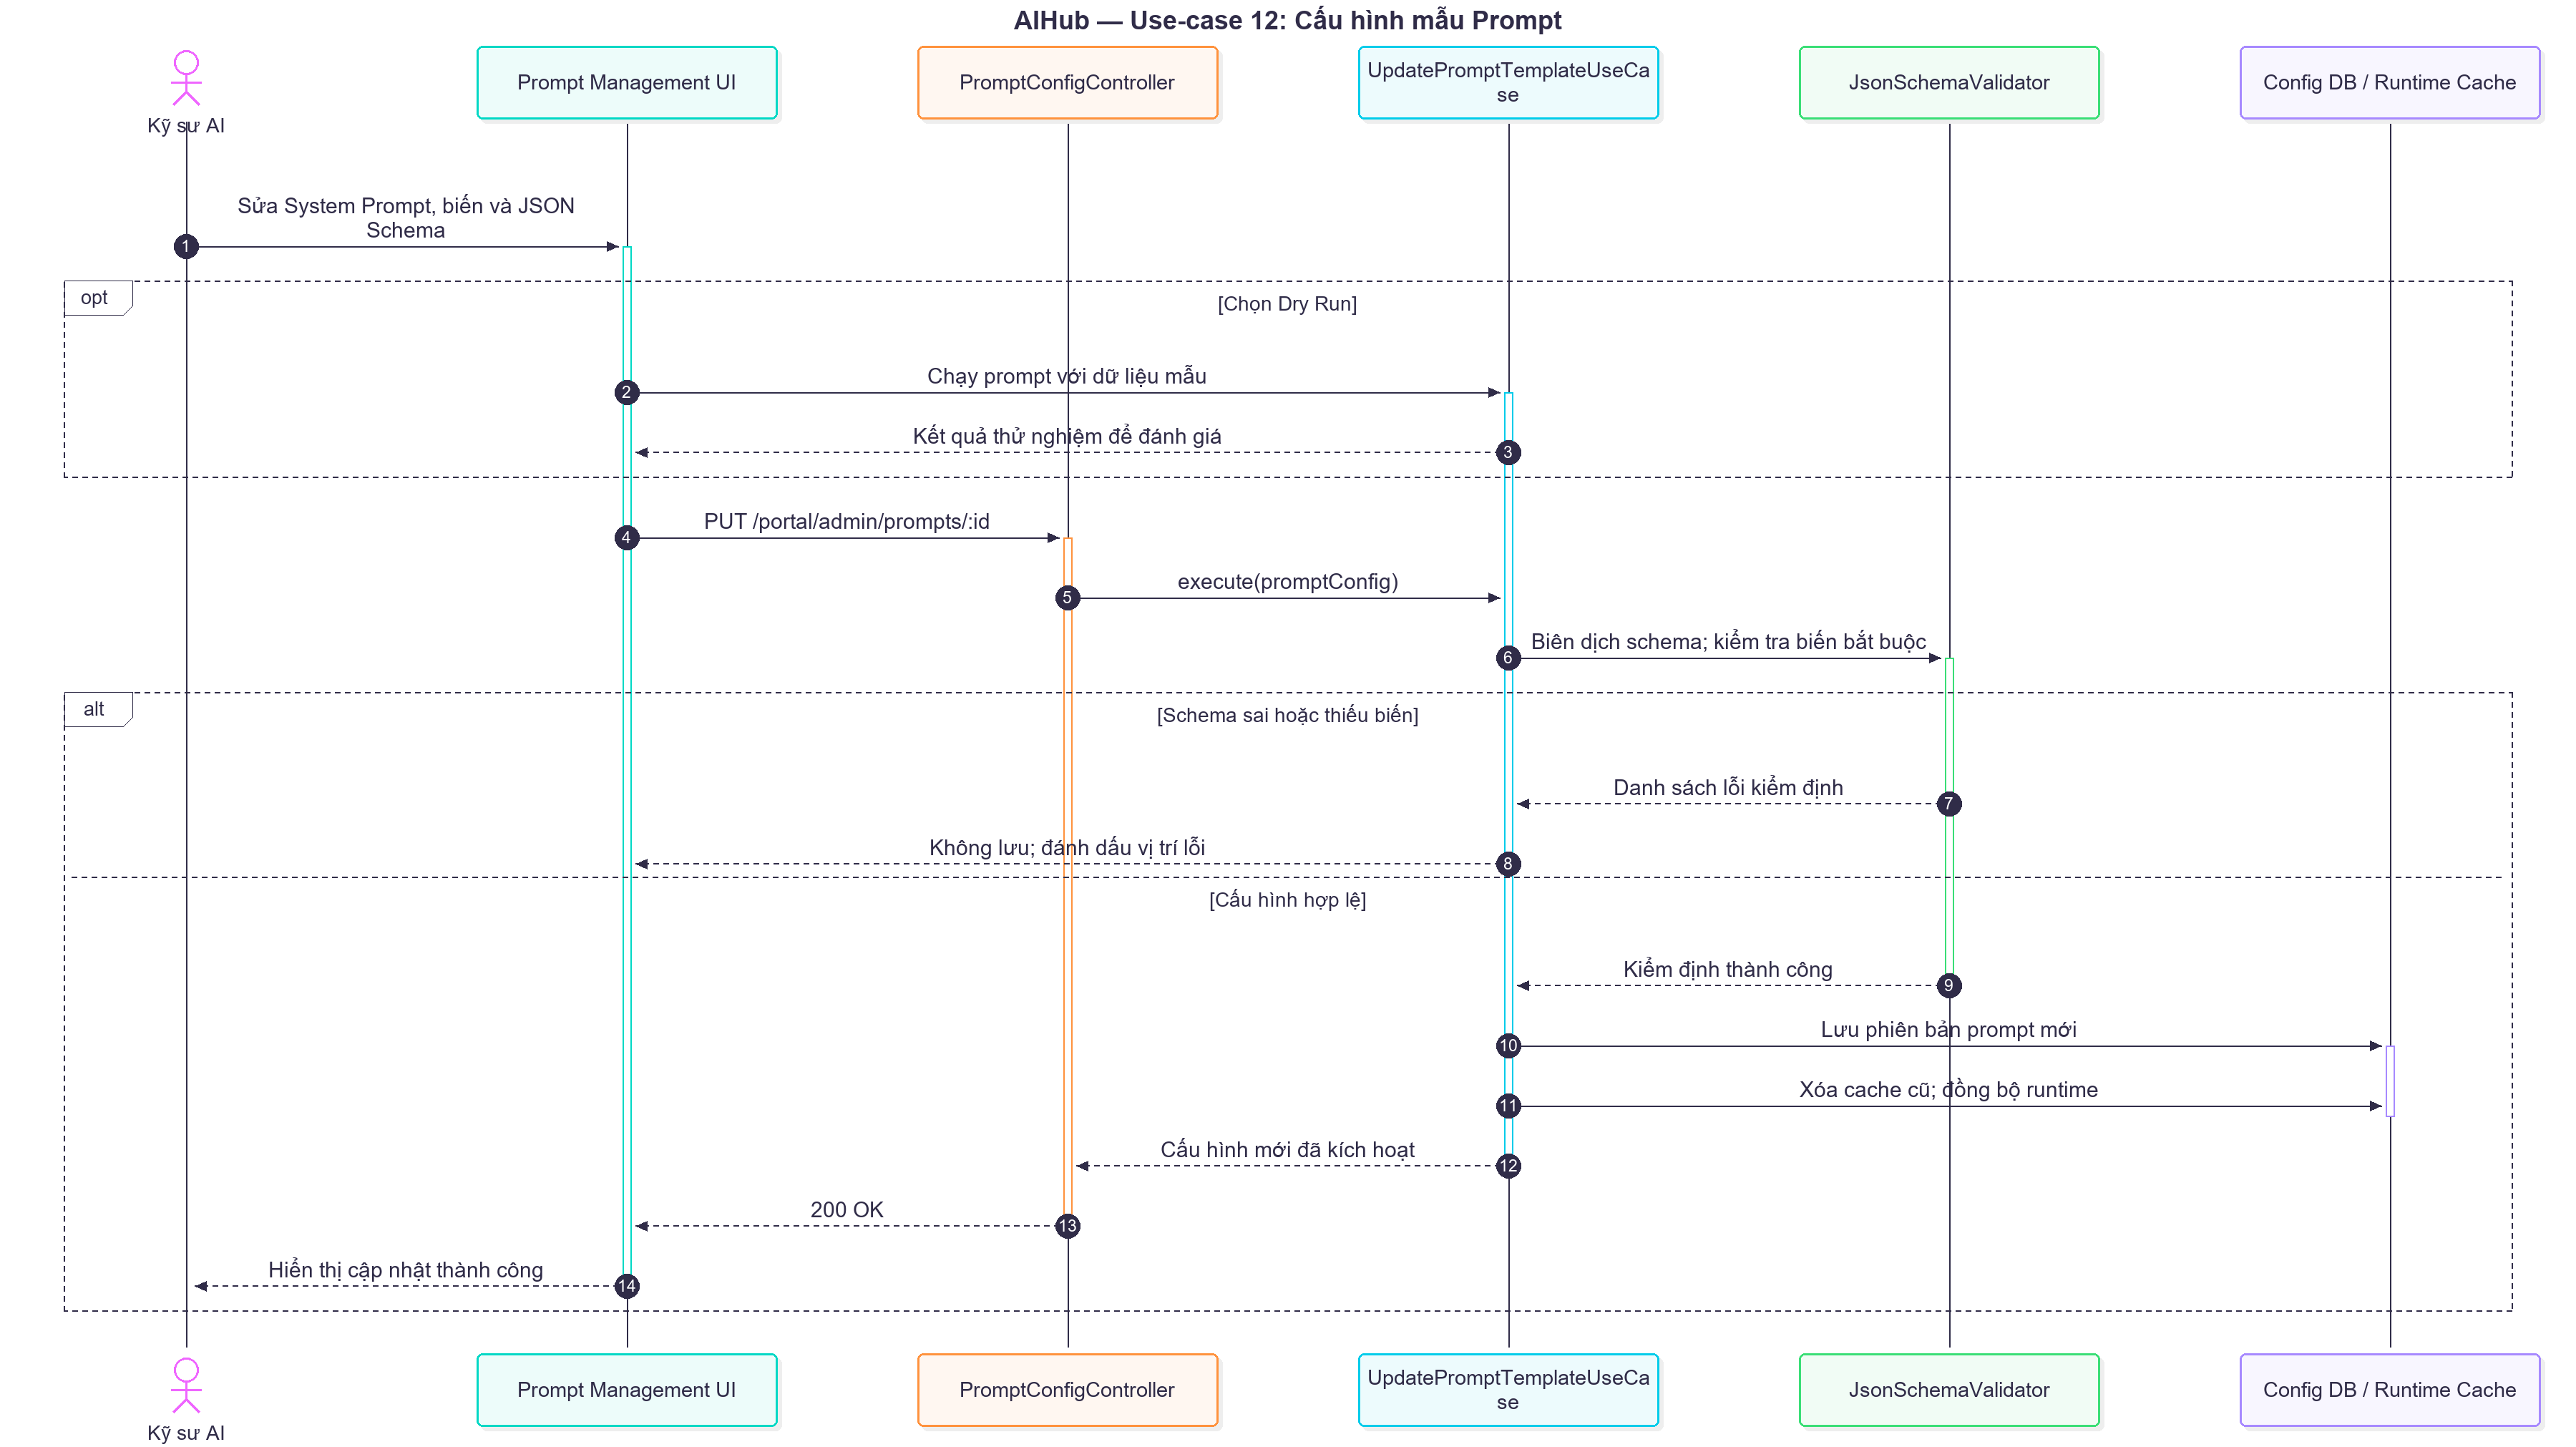
\includegraphics[width=\linewidth,height=.77\textheight,keepaspectratio]{Images/Sequence/AIHub/sequence_uc12_prompt_templates.png}
\caption{Sequence diagram AIHub UC12 — Cấu hình mẫu Prompt}
\label{sequence:aihub:sequence_uc12_prompt_templates}
\end{figure}

Dry Run không xuất bản cấu hình; Prompt được lưu phiên bản để bảo toàn khả năng truy vết mẫu.

\clearpage
\paragraph*{UC13. Cấu hình chuỗi mô hình dự phòng}

\begin{figure}[H]
\centering
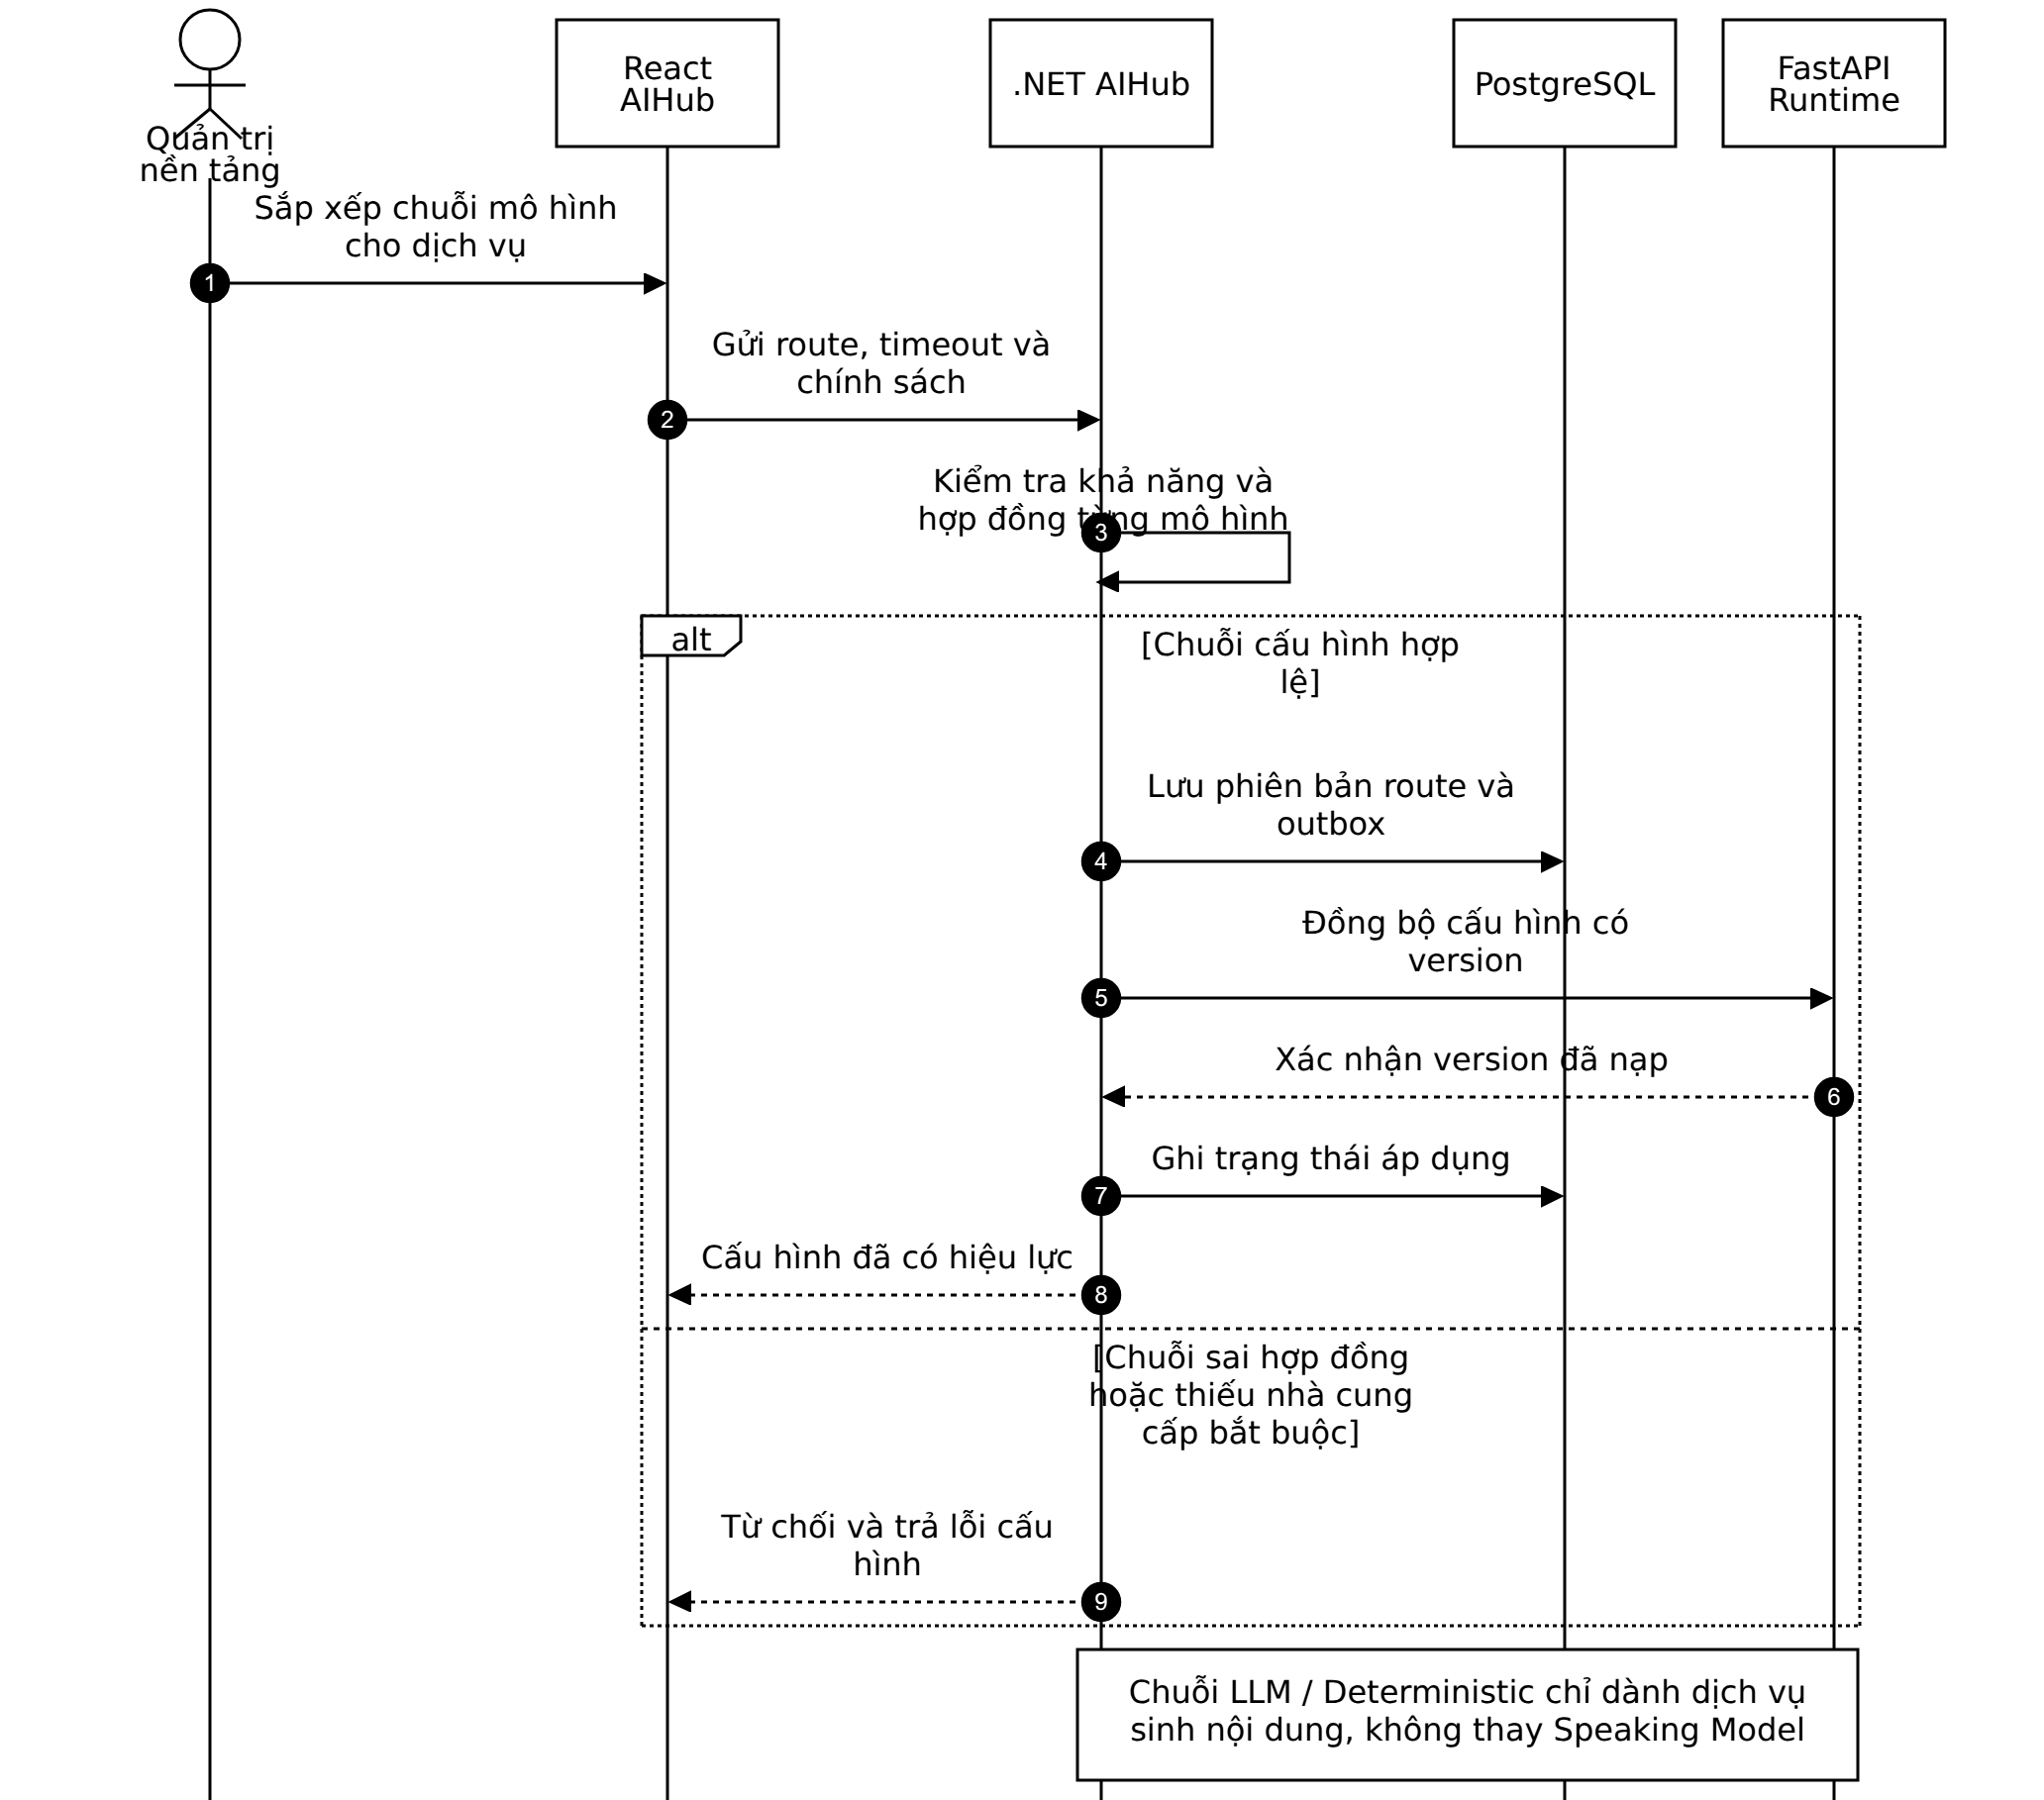
\includegraphics[width=\linewidth,height=.77\textheight,keepaspectratio]{Images/Sequence/AIHub/sequence_uc13_model_fallback.png}
\caption{Sequence diagram AIHub UC13 — Cấu hình chuỗi mô hình dự phòng}
\label{sequence:aihub:sequence_uc13_model_fallback}
\end{figure}

Chỉ công bố route đã kiểm định; dự phòng cho sinh nội dung không mặc nhiên thay thế mô hình chấm Speaking.

\clearpage
\paragraph*{UC14. Xuất dữ liệu SFT và DPO}

\begin{figure}[H]
\centering
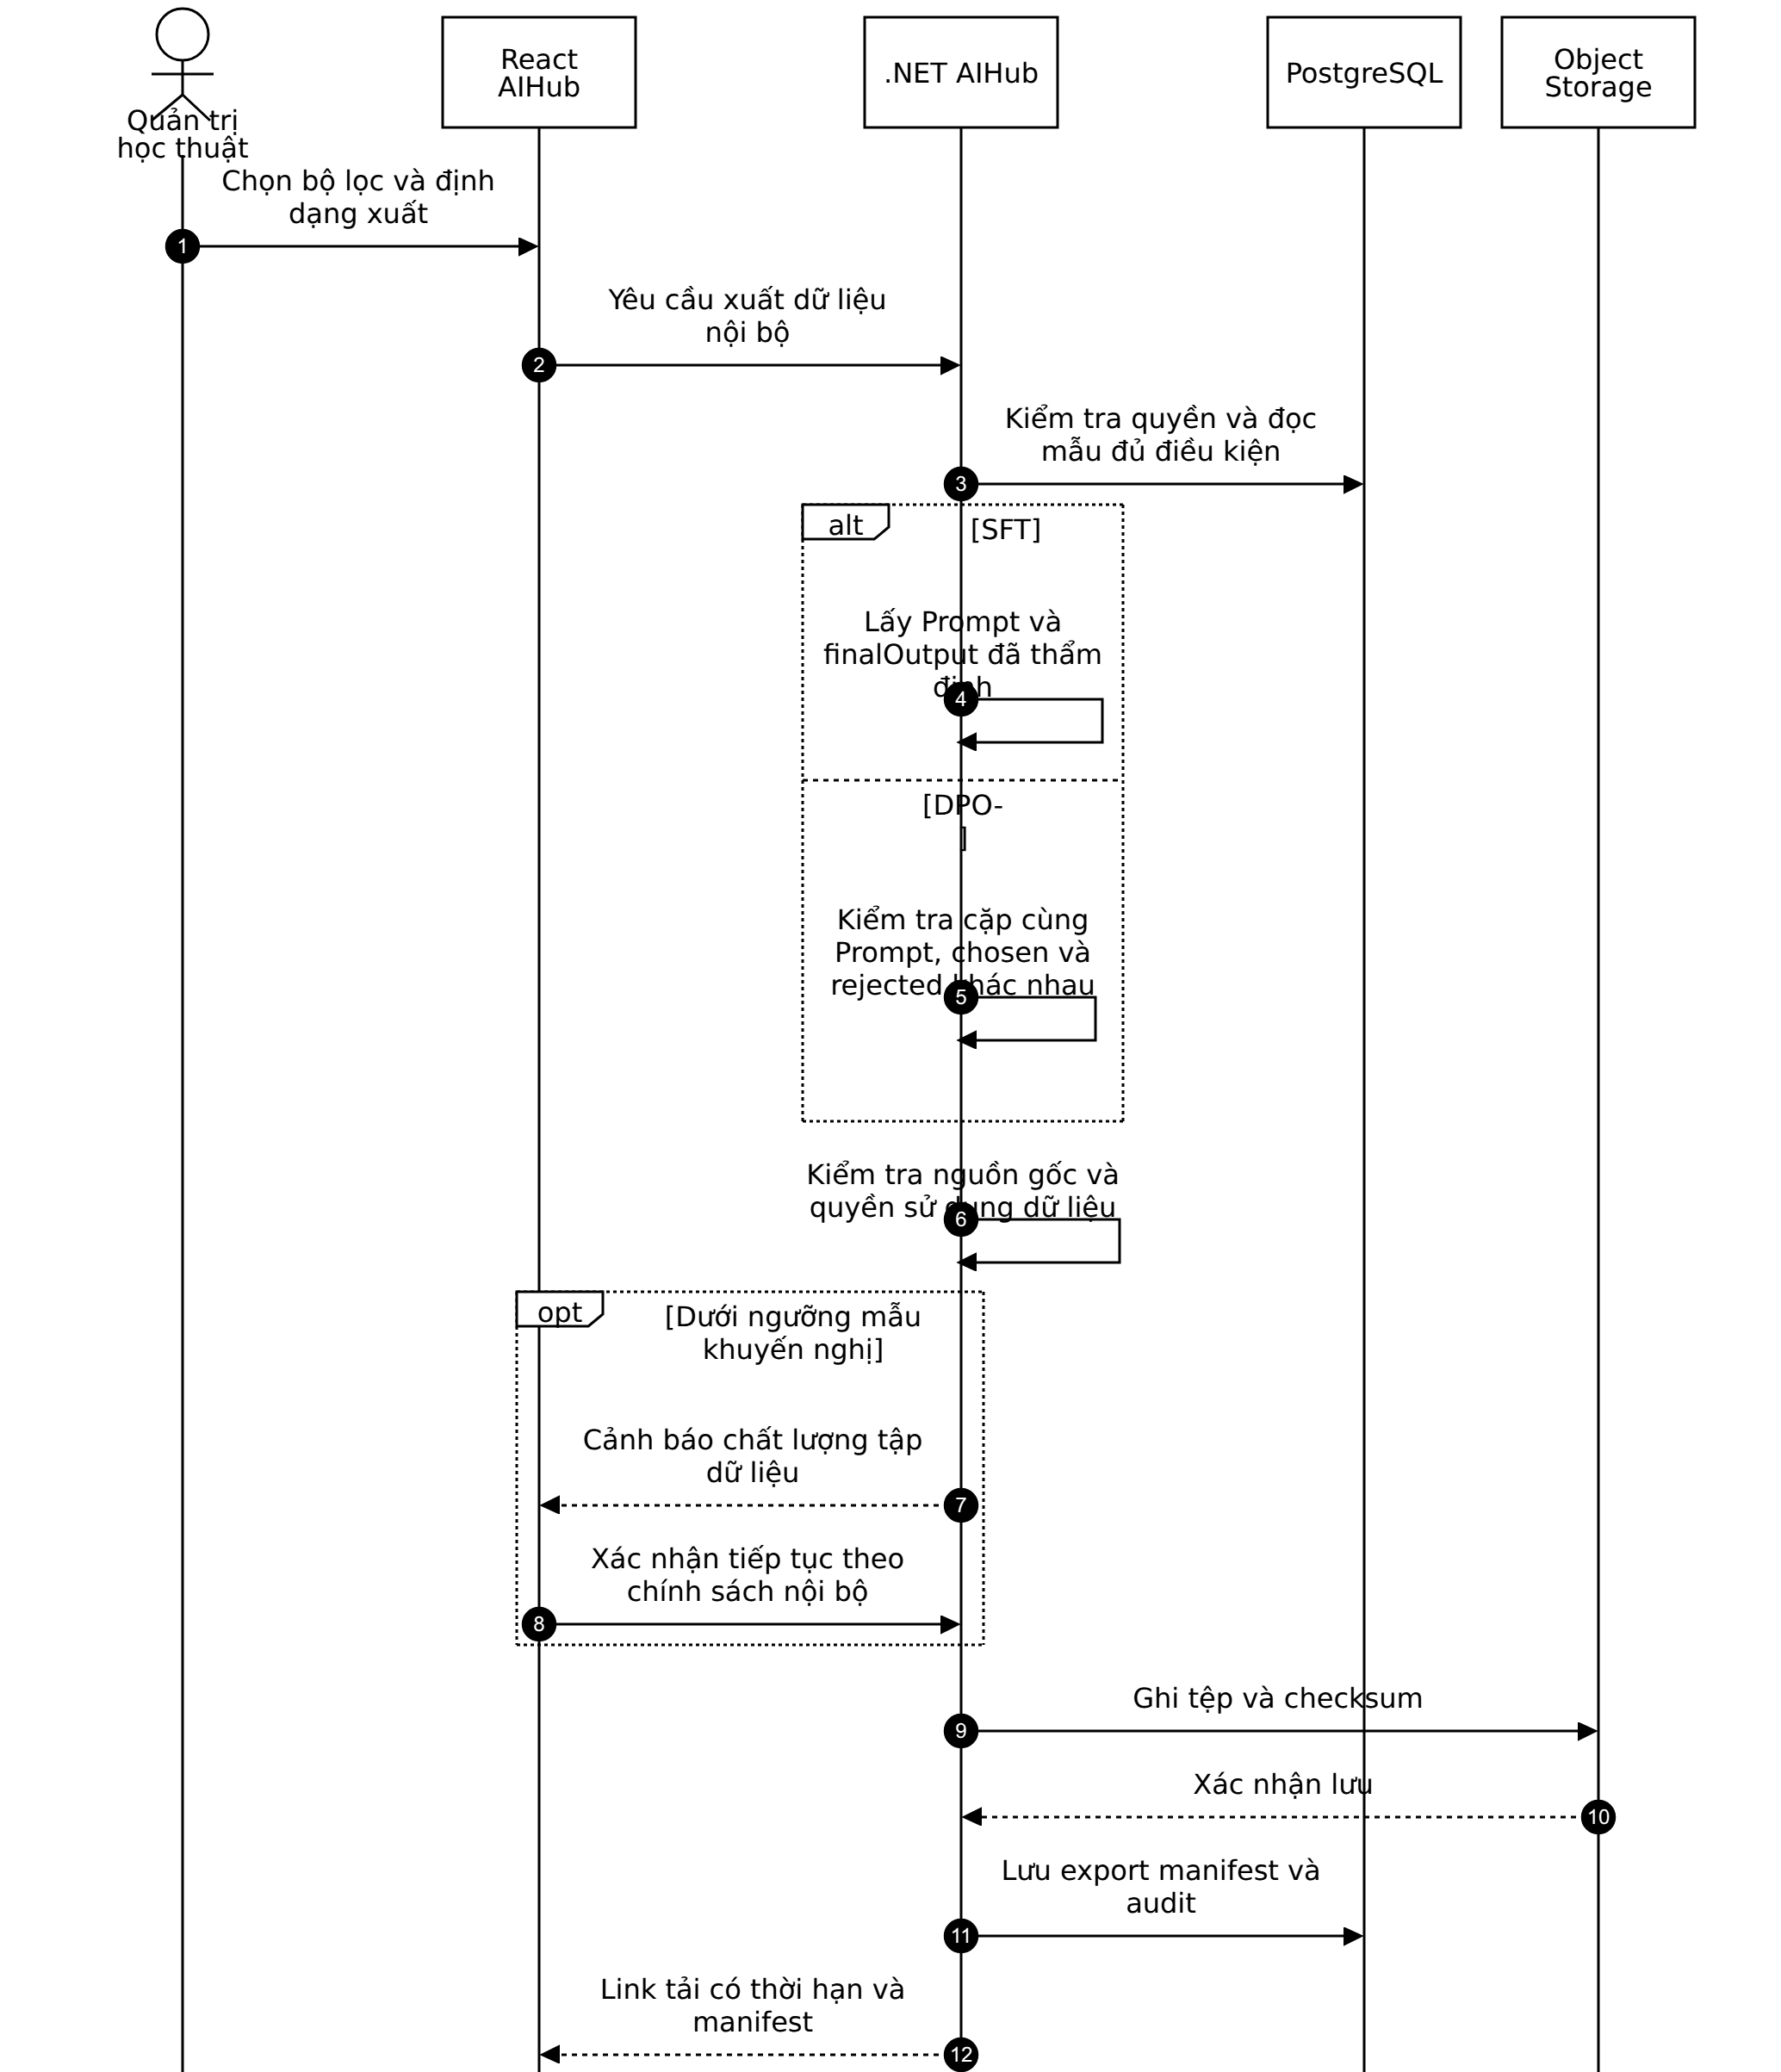
\includegraphics[width=\linewidth,height=.77\textheight,keepaspectratio]{Images/Sequence/AIHub/sequence_uc14_export_datasets.png}
\caption{Sequence diagram AIHub UC14 — Xuất dữ liệu SFT và DPO}
\label{sequence:aihub:sequence_uc14_export_datasets}
\end{figure}

Xuất dữ liệu kiểm tra nguồn gốc và cấu trúc cặp; manifest lưu đầy đủ mẫu và phiên bản được chọn.

\clearpage
\paragraph*{UC15. Phân tích lỗi mô hình}

\begin{figure}[H]
\centering
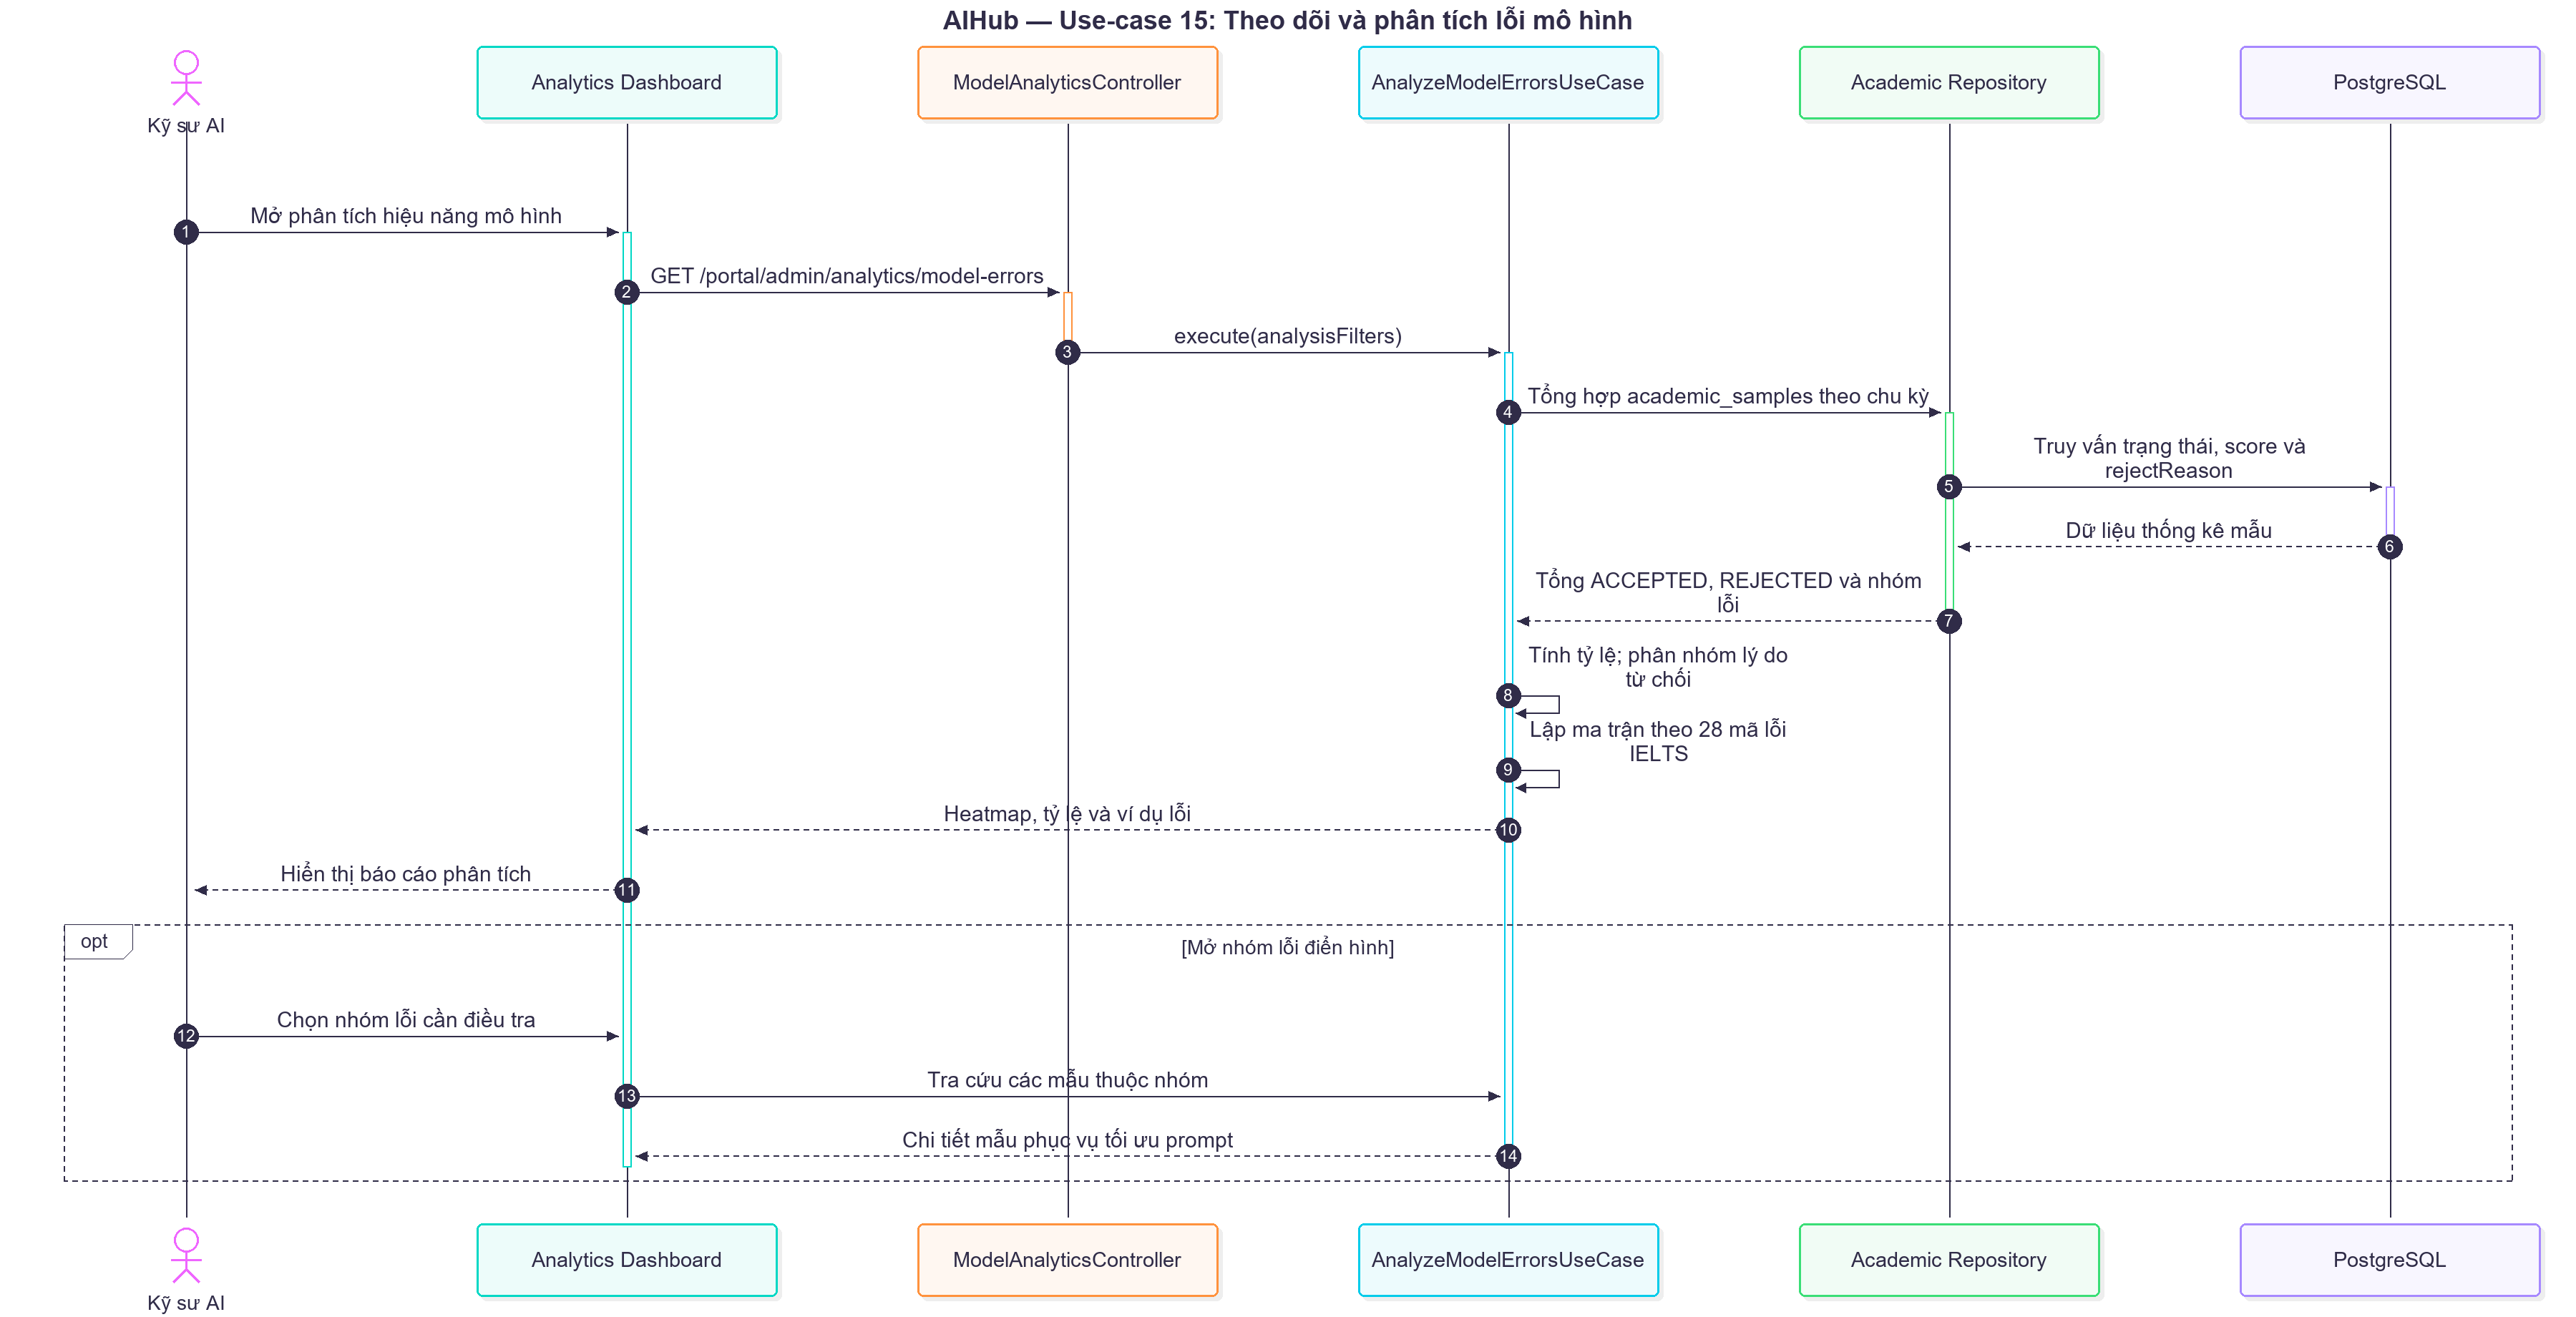
\includegraphics[width=\linewidth,height=.77\textheight,keepaspectratio]{Images/Sequence/AIHub/sequence_uc15_model_error_analysis.png}
\caption{Sequence diagram AIHub UC15 — Phân tích lỗi mô hình}
\label{sequence:aihub:sequence_uc15_model_error_analysis}
\end{figure}

Thống kê thể hiện số mẫu và phiên bản; mẫu nháp không làm sai mẫu số của tỷ lệ thẩm định.

\clearpage
\paragraph*{UC16. Quản lý thành viên tổ chức}

\begin{figure}[H]
\centering
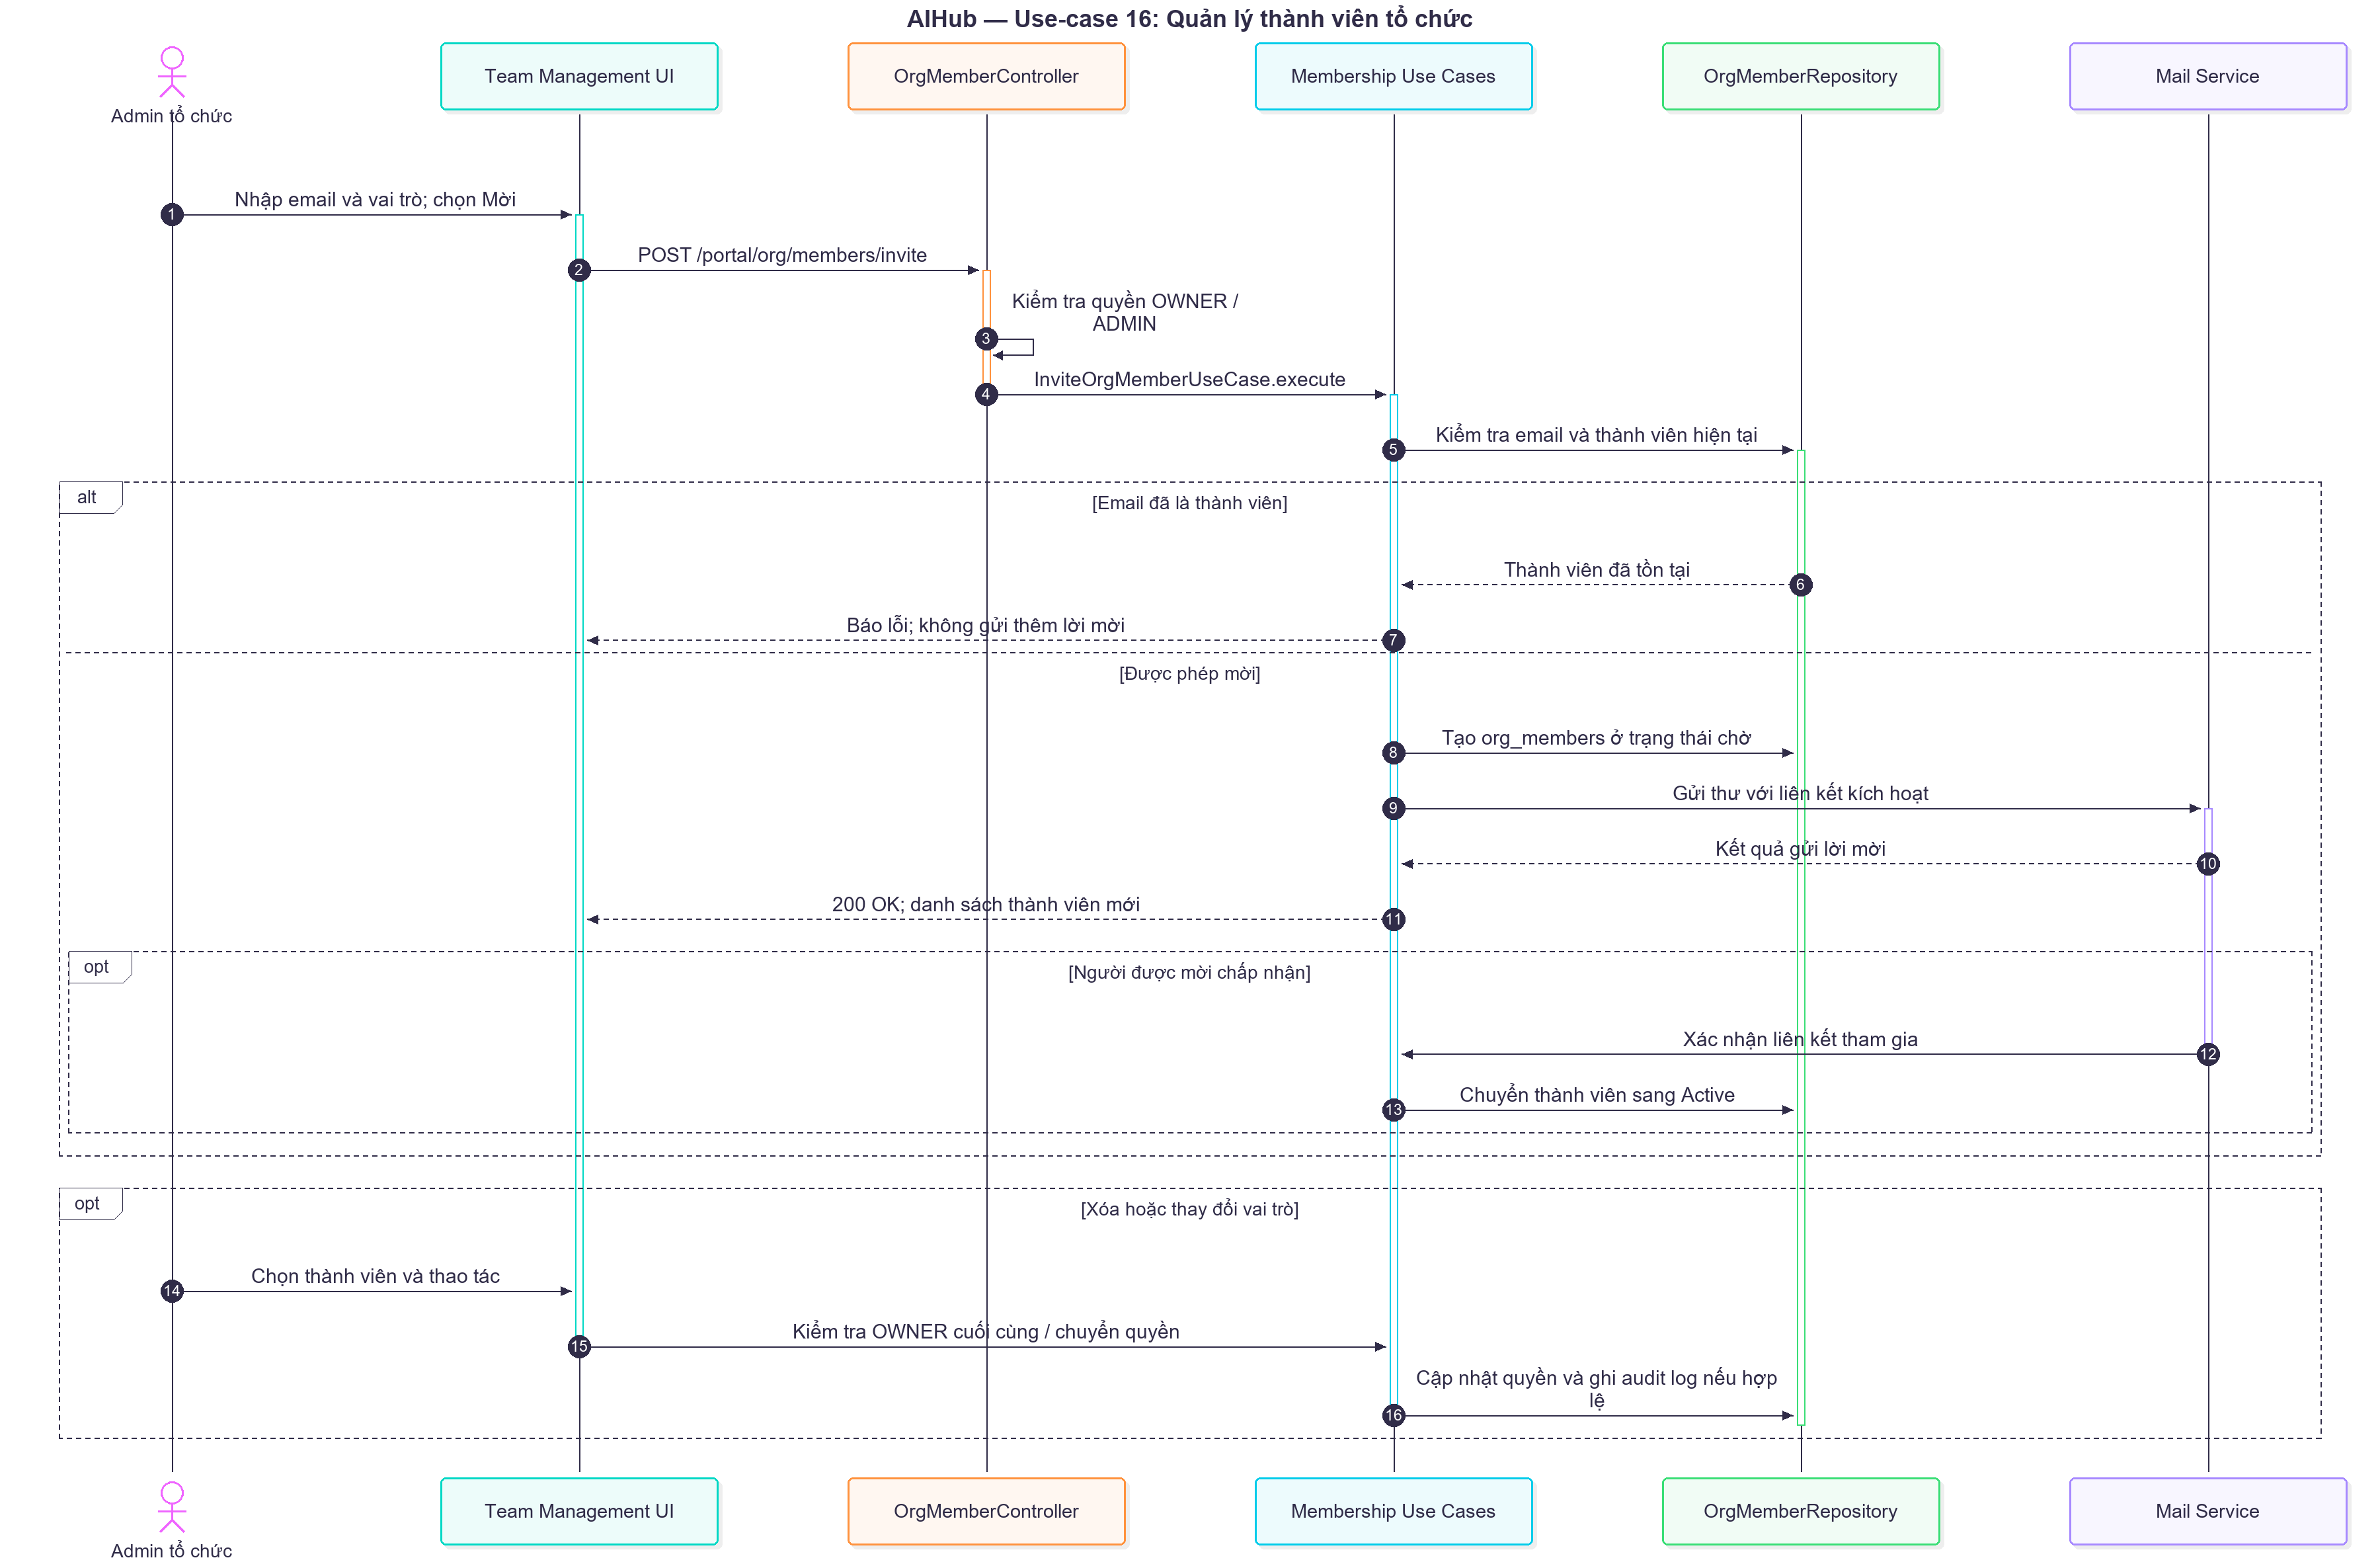
\includegraphics[width=\linewidth,height=.77\textheight,keepaspectratio]{Images/Sequence/AIHub/sequence_uc16_organization_members.png}
\caption{Sequence diagram AIHub UC16 — Quản lý thành viên tổ chức}
\label{sequence:aihub:sequence_uc16_organization_members}
\end{figure}

Mọi thay đổi giới hạn theo tổ chức; chuyển Owner là giao dịch có xác thực bổ sung và không để mất Owner.

\clearpage
\paragraph*{UC17. Quản trị gói và hạn mức}

\begin{figure}[H]
\centering
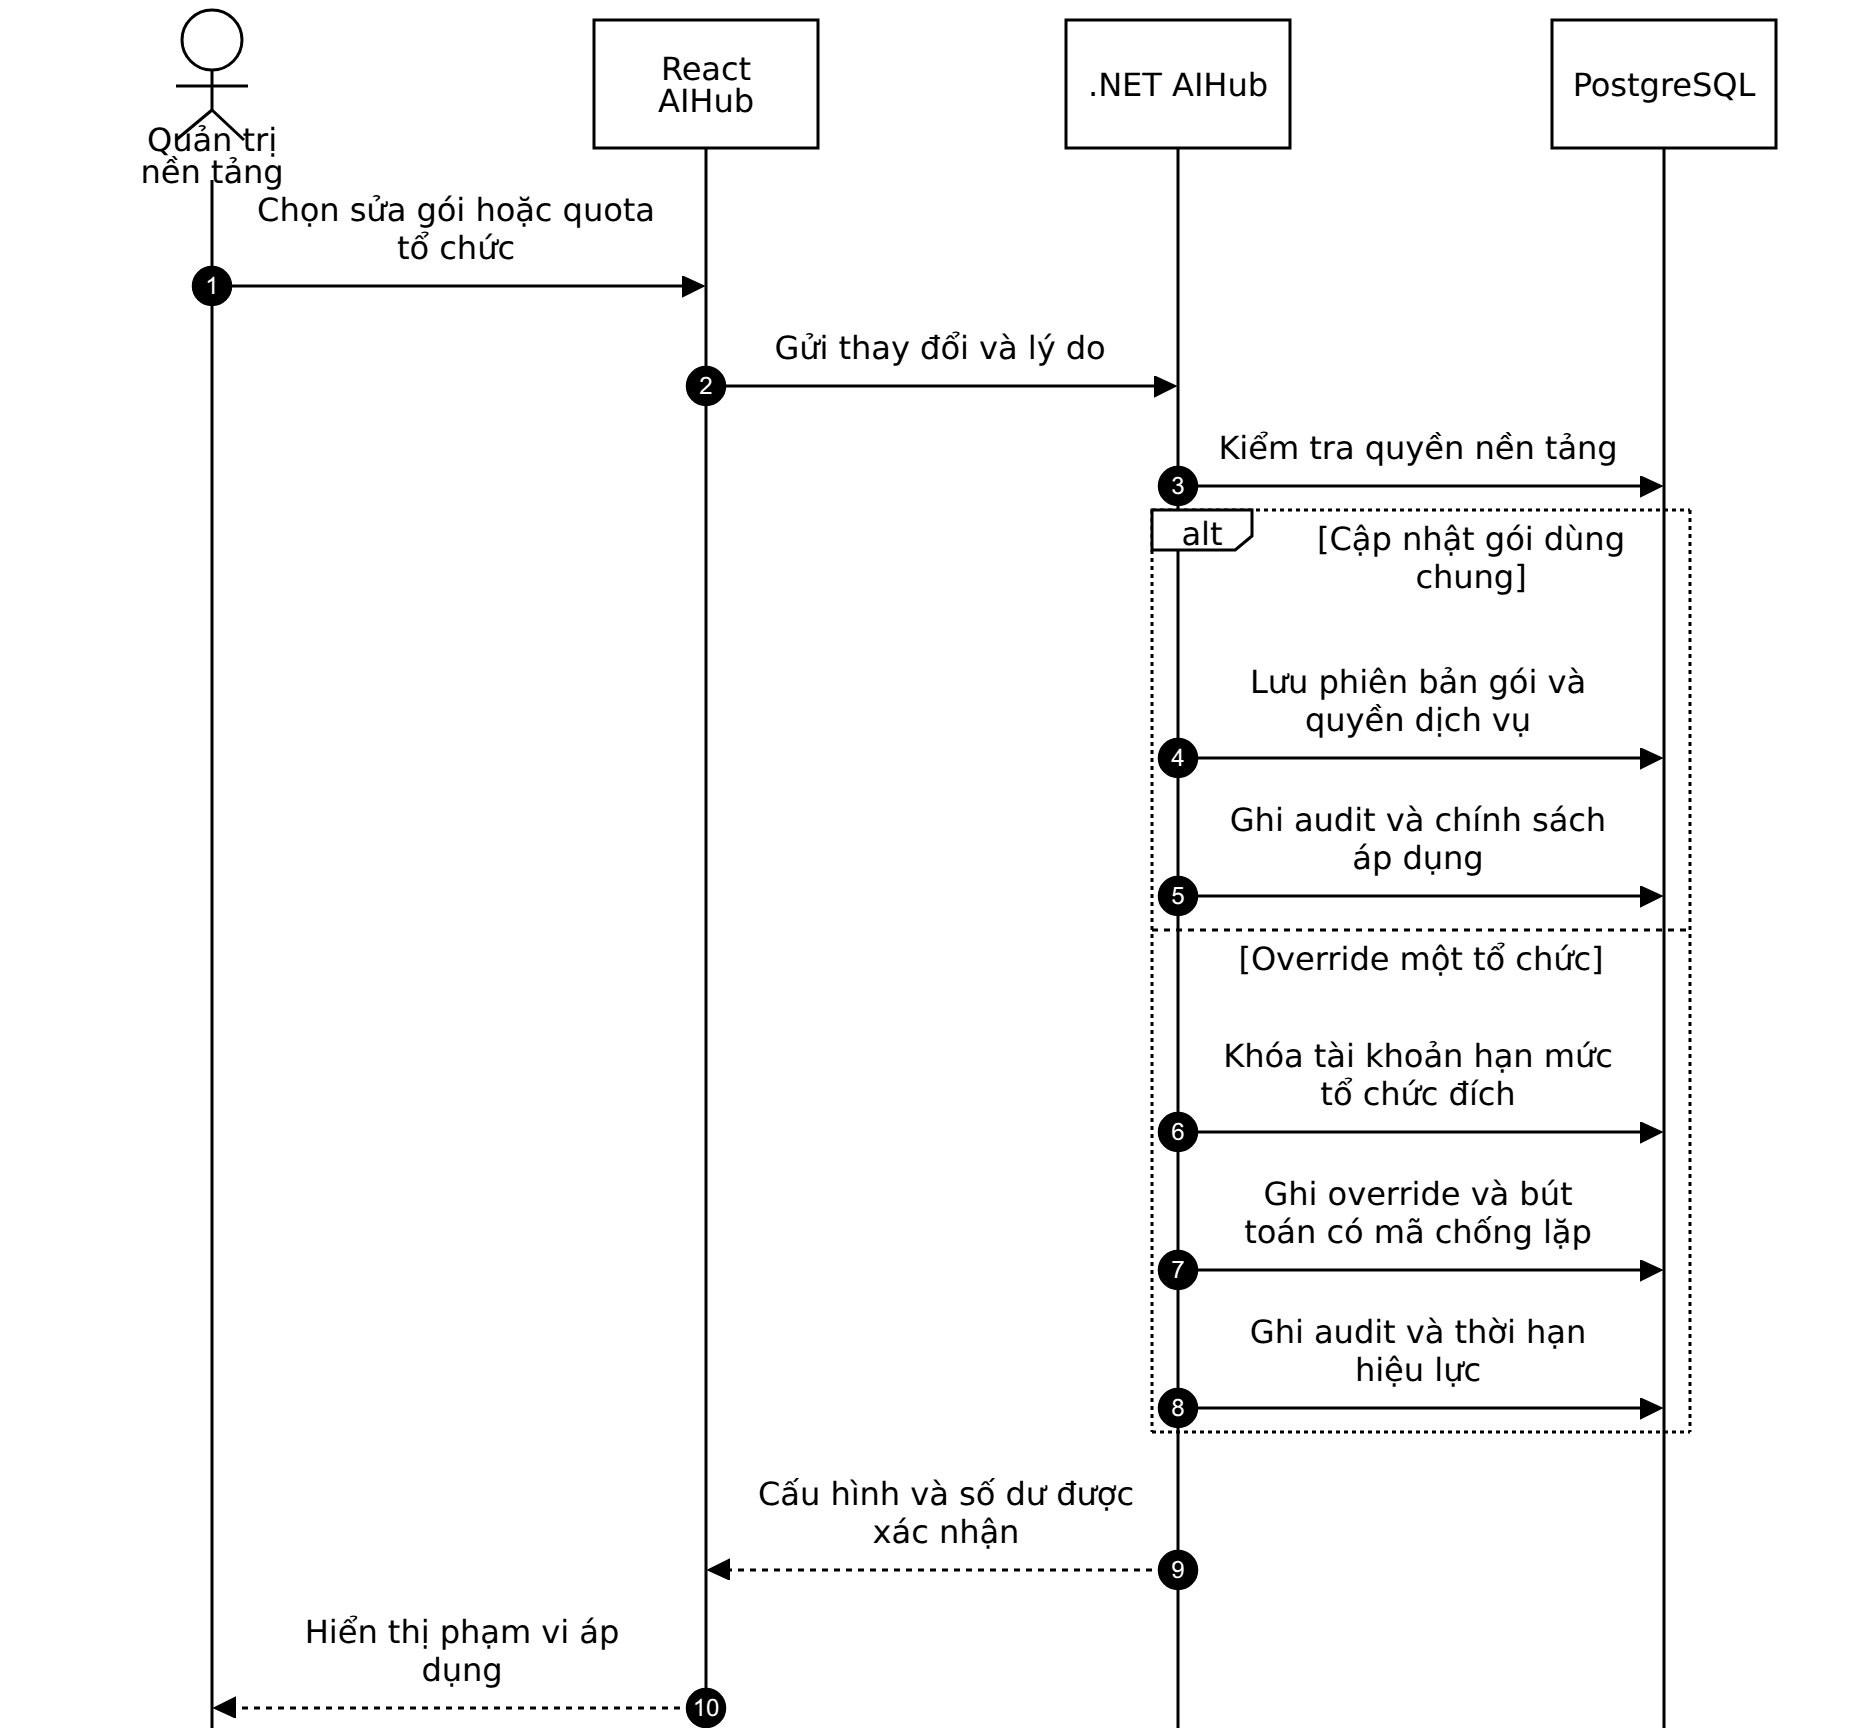
\includegraphics[width=\linewidth,height=.77\textheight,keepaspectratio]{Images/Sequence/AIHub/sequence_uc17_plans_quota.png}
\caption{Sequence diagram AIHub UC17 — Quản trị gói và hạn mức}
\label{sequence:aihub:sequence_uc17_plans_quota}
\end{figure}

Cập nhật gói và override là hai nghiệp vụ khác nhau; override không tác động số dư của tổ chức khác.

\clearpage
\paragraph*{UC18. Giám sát trạng thái hệ thống}

\begin{figure}[H]
\centering
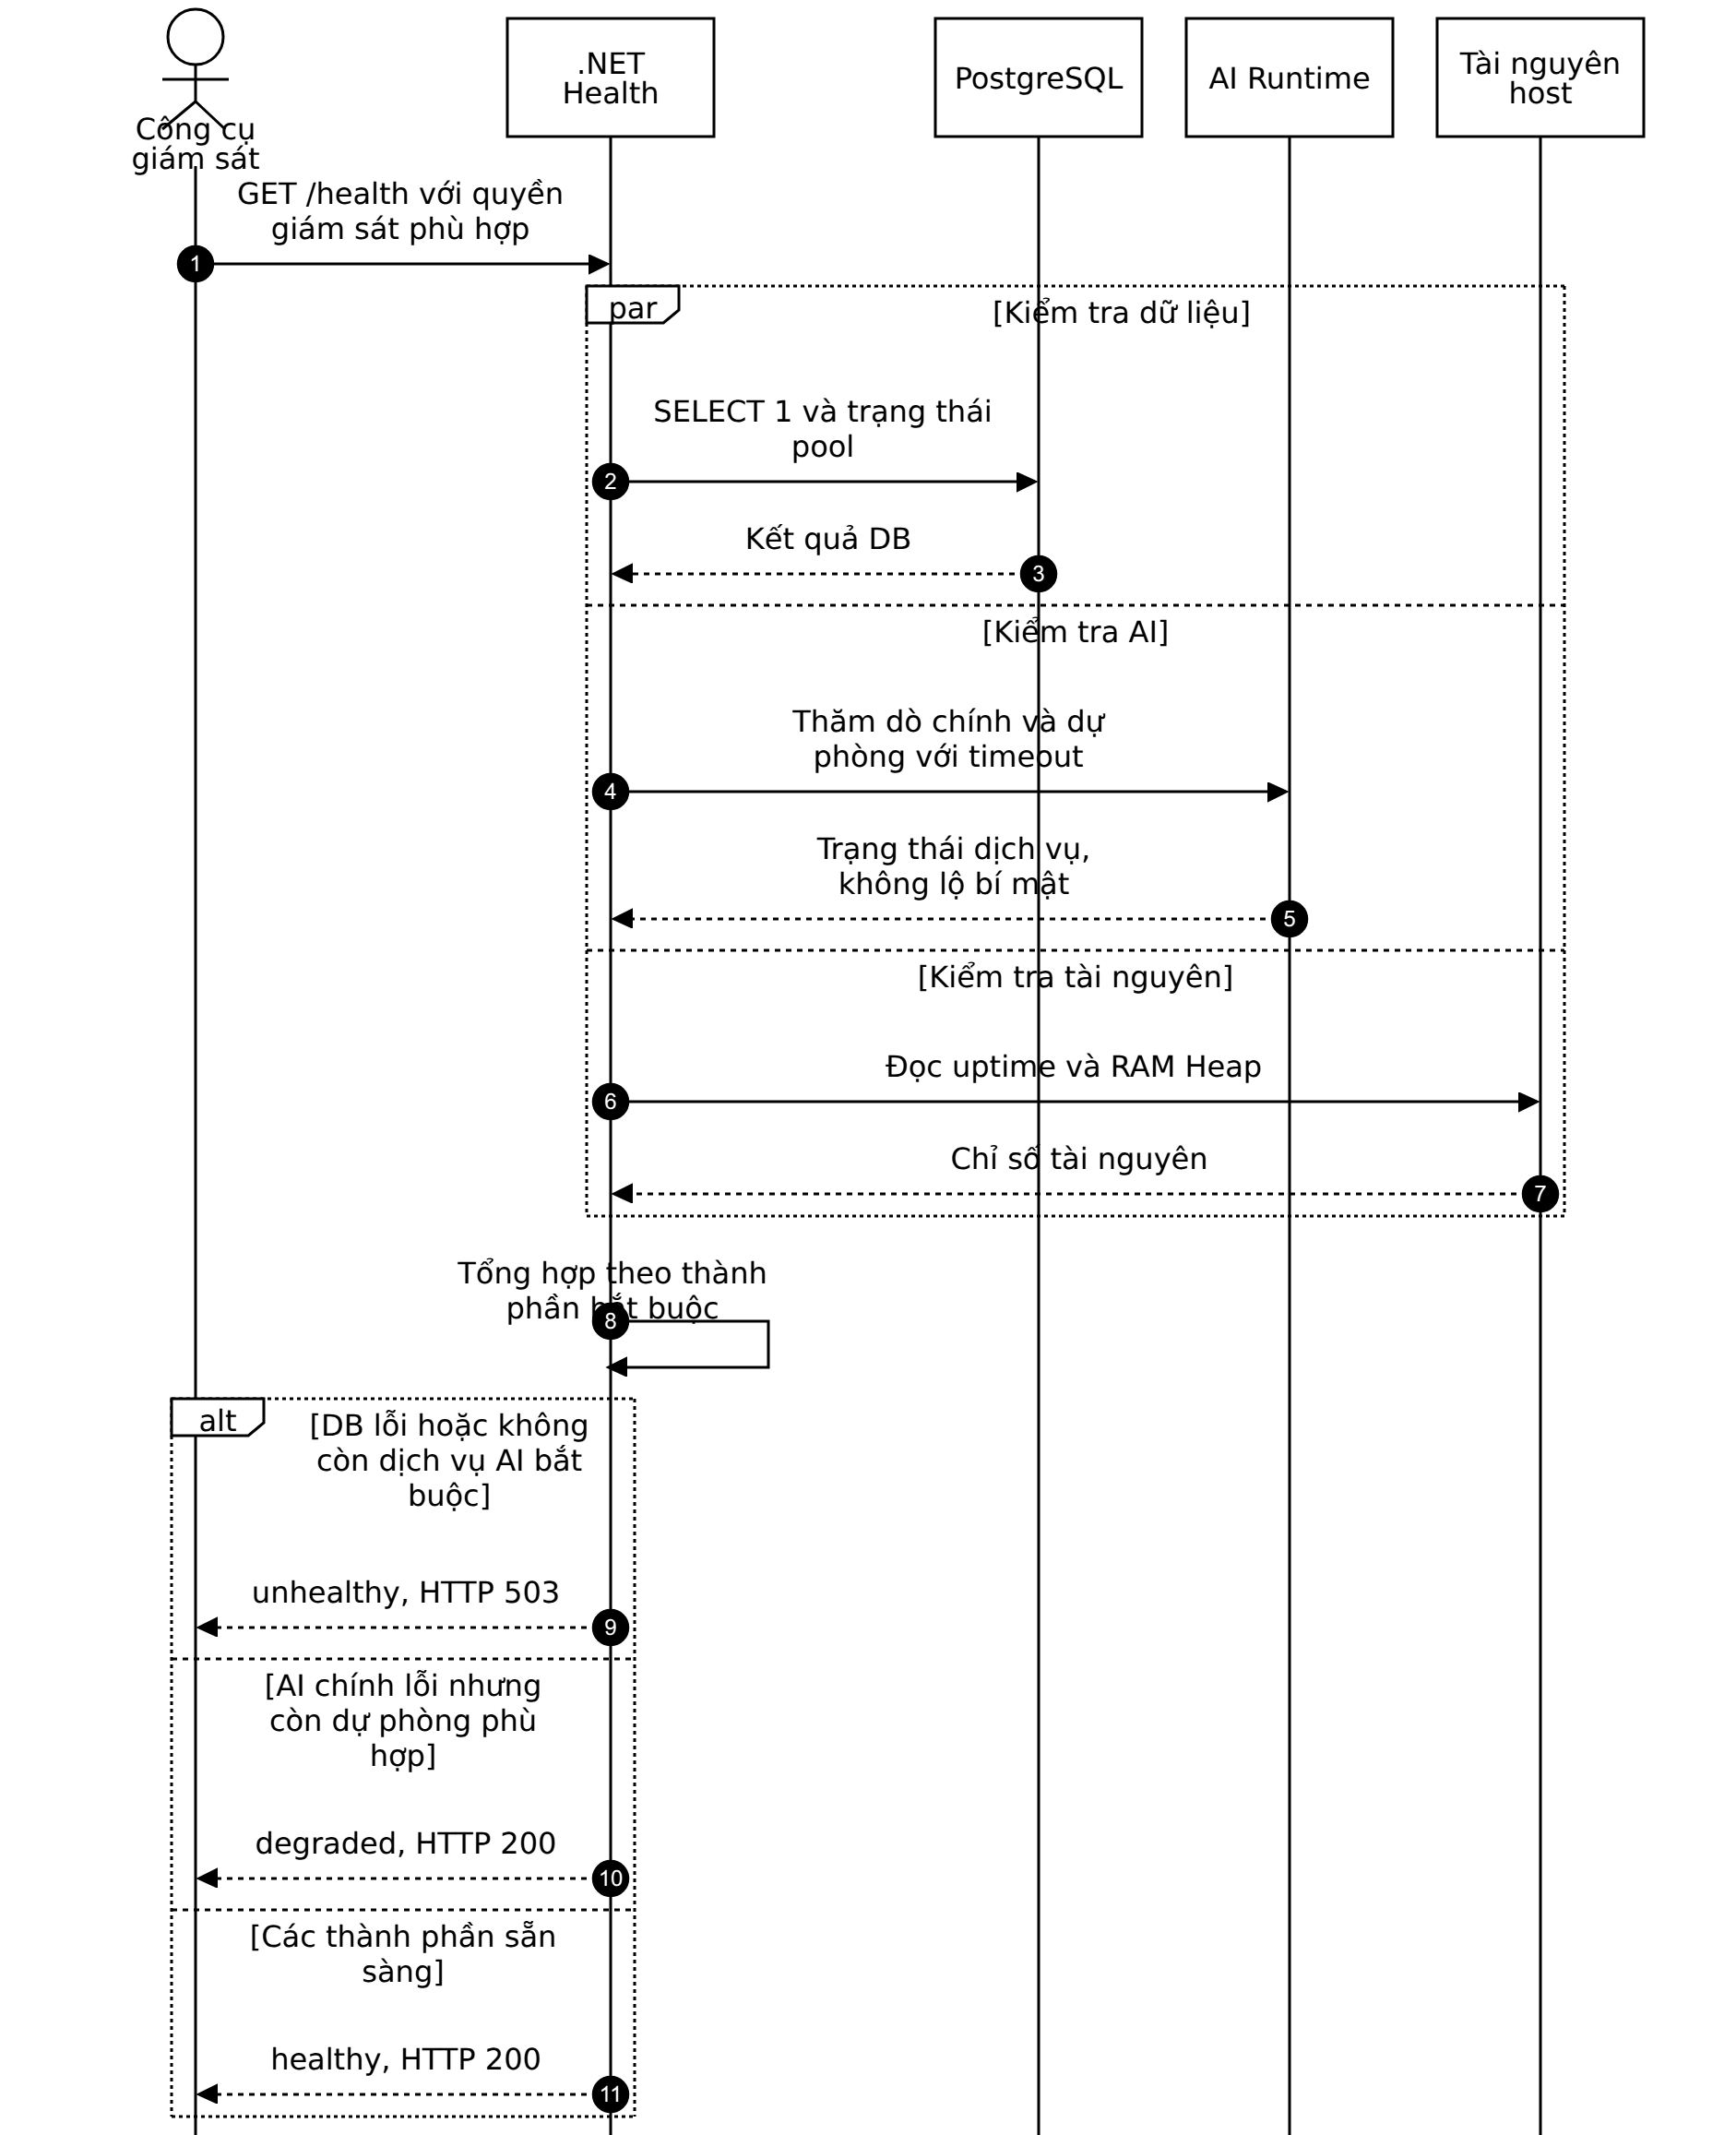
\includegraphics[width=\linewidth,height=.77\textheight,keepaspectratio]{Images/Sequence/AIHub/sequence_uc18_system_health.png}
\caption{Sequence diagram AIHub UC18 — Giám sát trạng thái hệ thống}
\label{sequence:aihub:sequence_uc18_system_health}
\end{figure}

Health tổng hợp kiểm tra có timeout; trạng thái degraded chỉ hợp lệ khi còn phương án thực sự đáp ứng hợp đồng dịch vụ.

\clearpage
\paragraph*{UC19. Quản lý Universal Specs}

\begin{figure}[H]
\centering
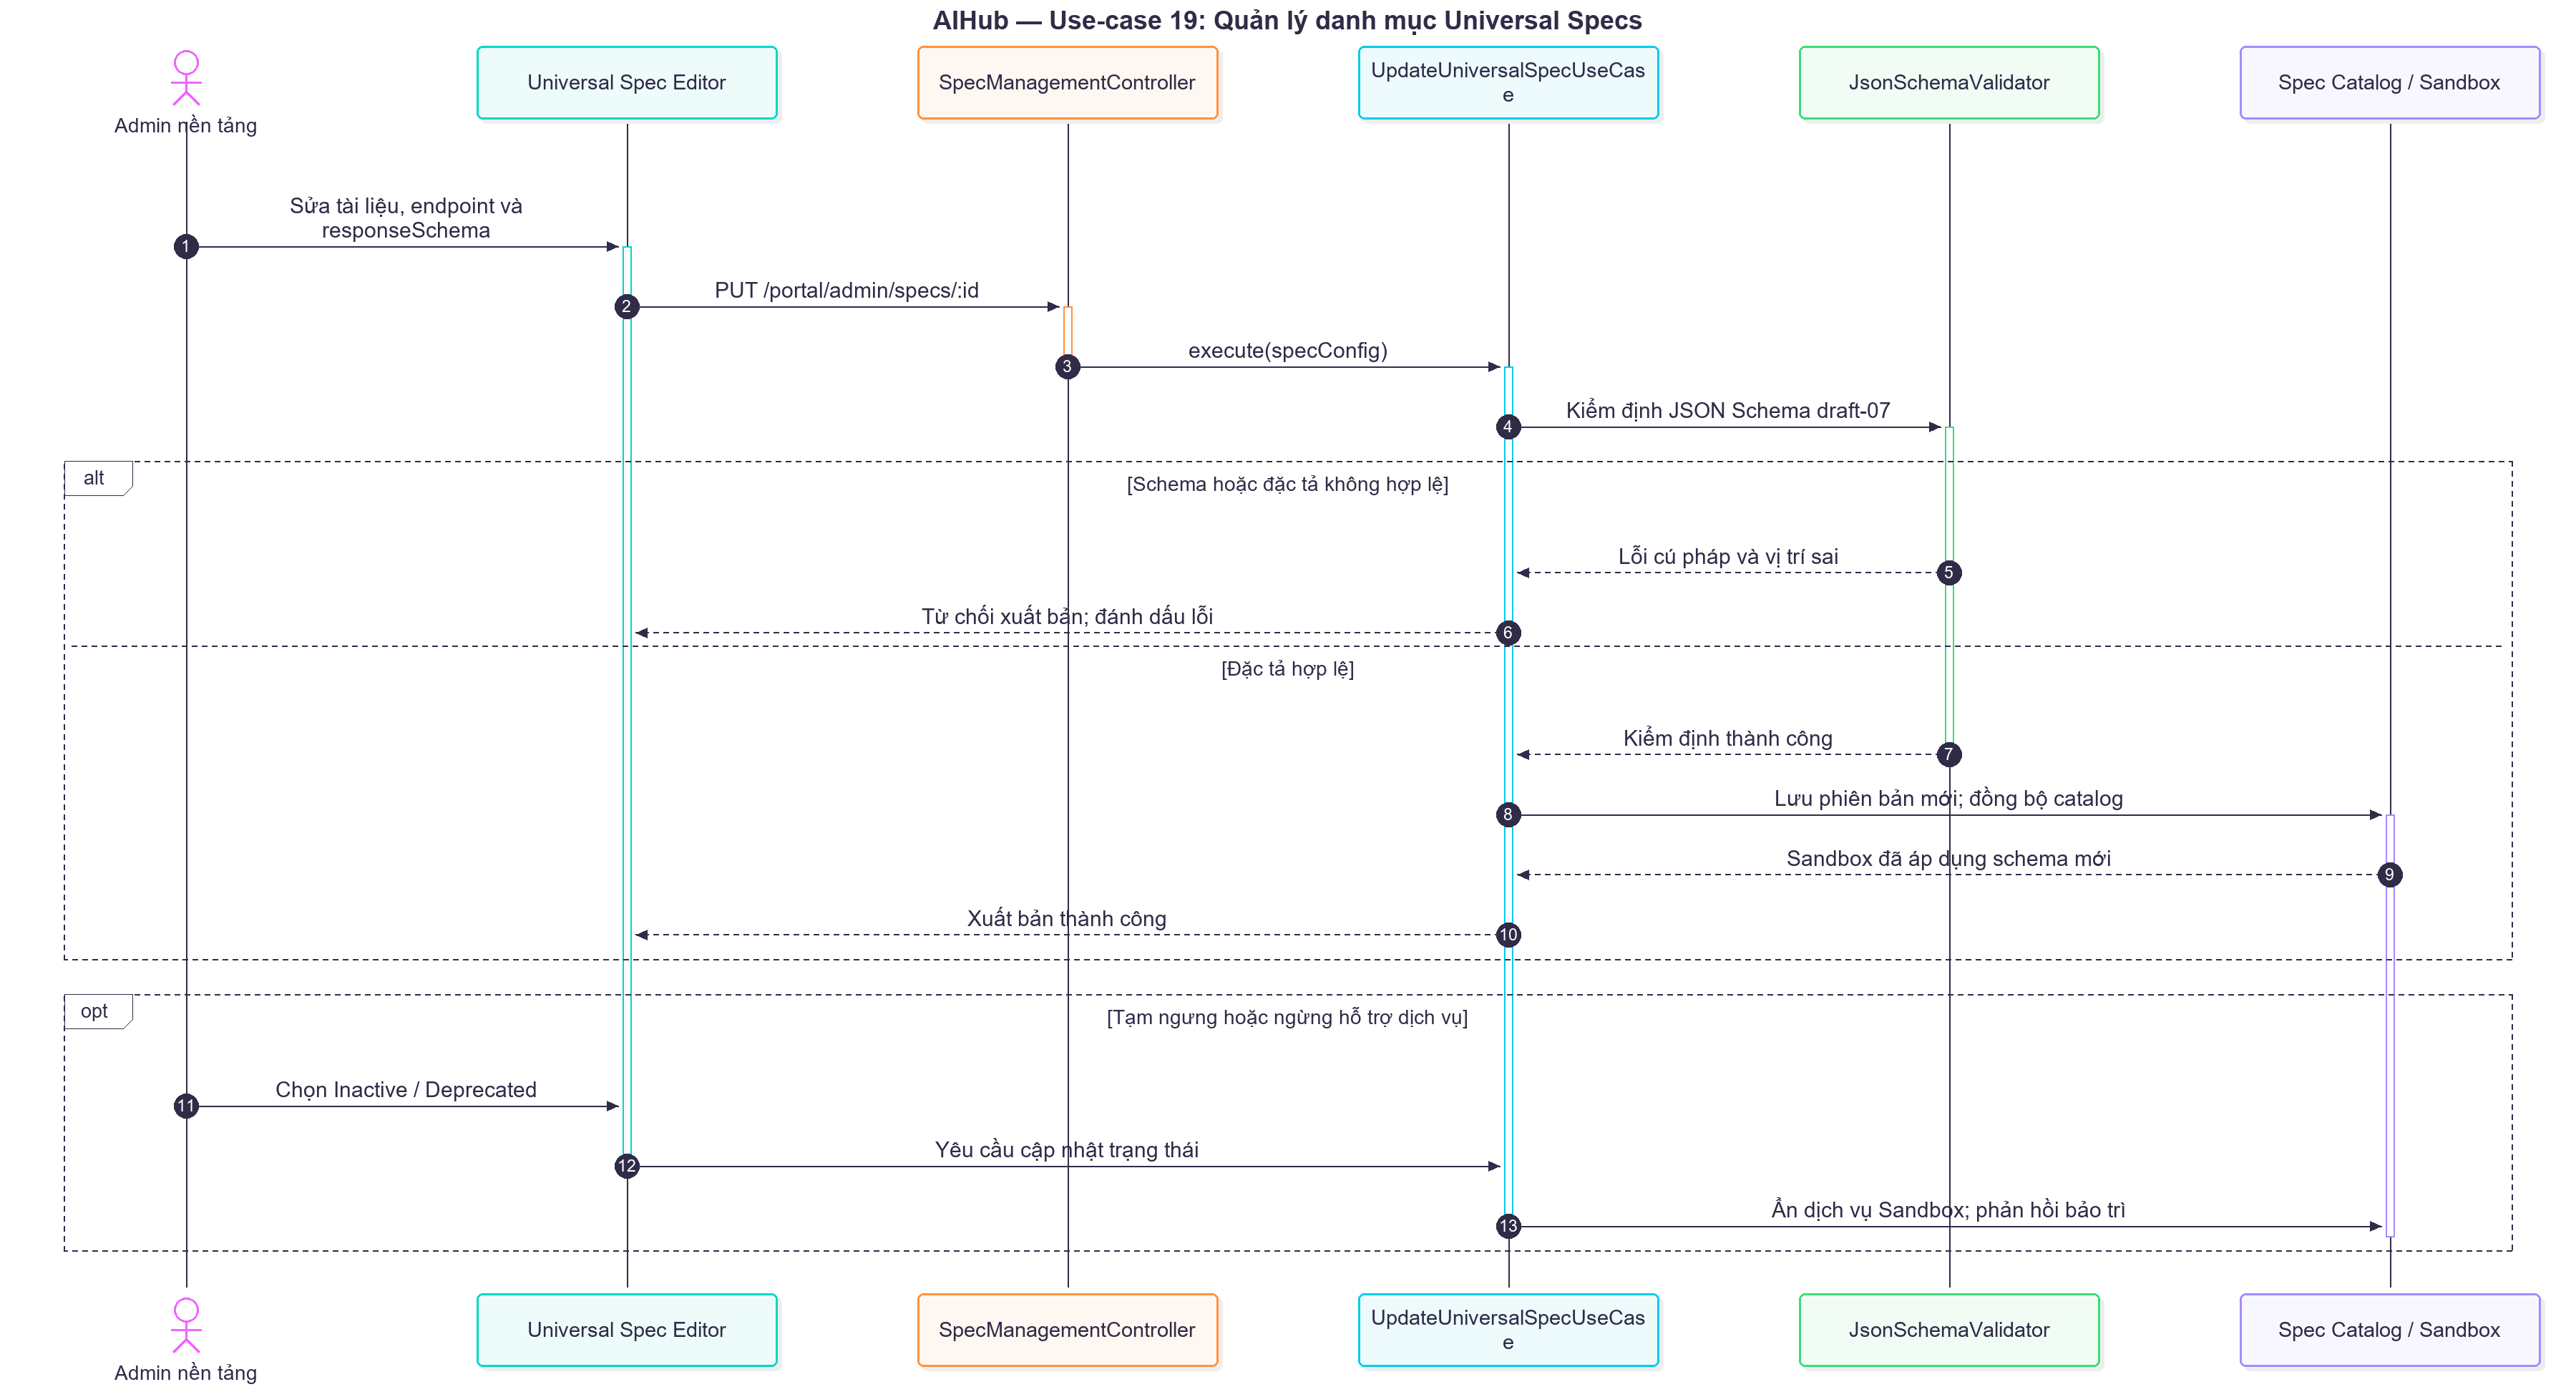
\includegraphics[width=\linewidth,height=.77\textheight,keepaspectratio]{Images/Sequence/AIHub/sequence_uc19_universal_specs.png}
\caption{Sequence diagram AIHub UC19 — Quản lý Universal Specs}
\label{sequence:aihub:sequence_uc19_universal_specs}
\end{figure}

Spec được version hóa và đồng bộ với Sandbox; phiên bản ngừng hoạt động không được sử dụng để chạy thử.

\clearpage
\paragraph*{UC20. Kiểm toán và truy vết giao dịch}

\begin{figure}[H]
\centering
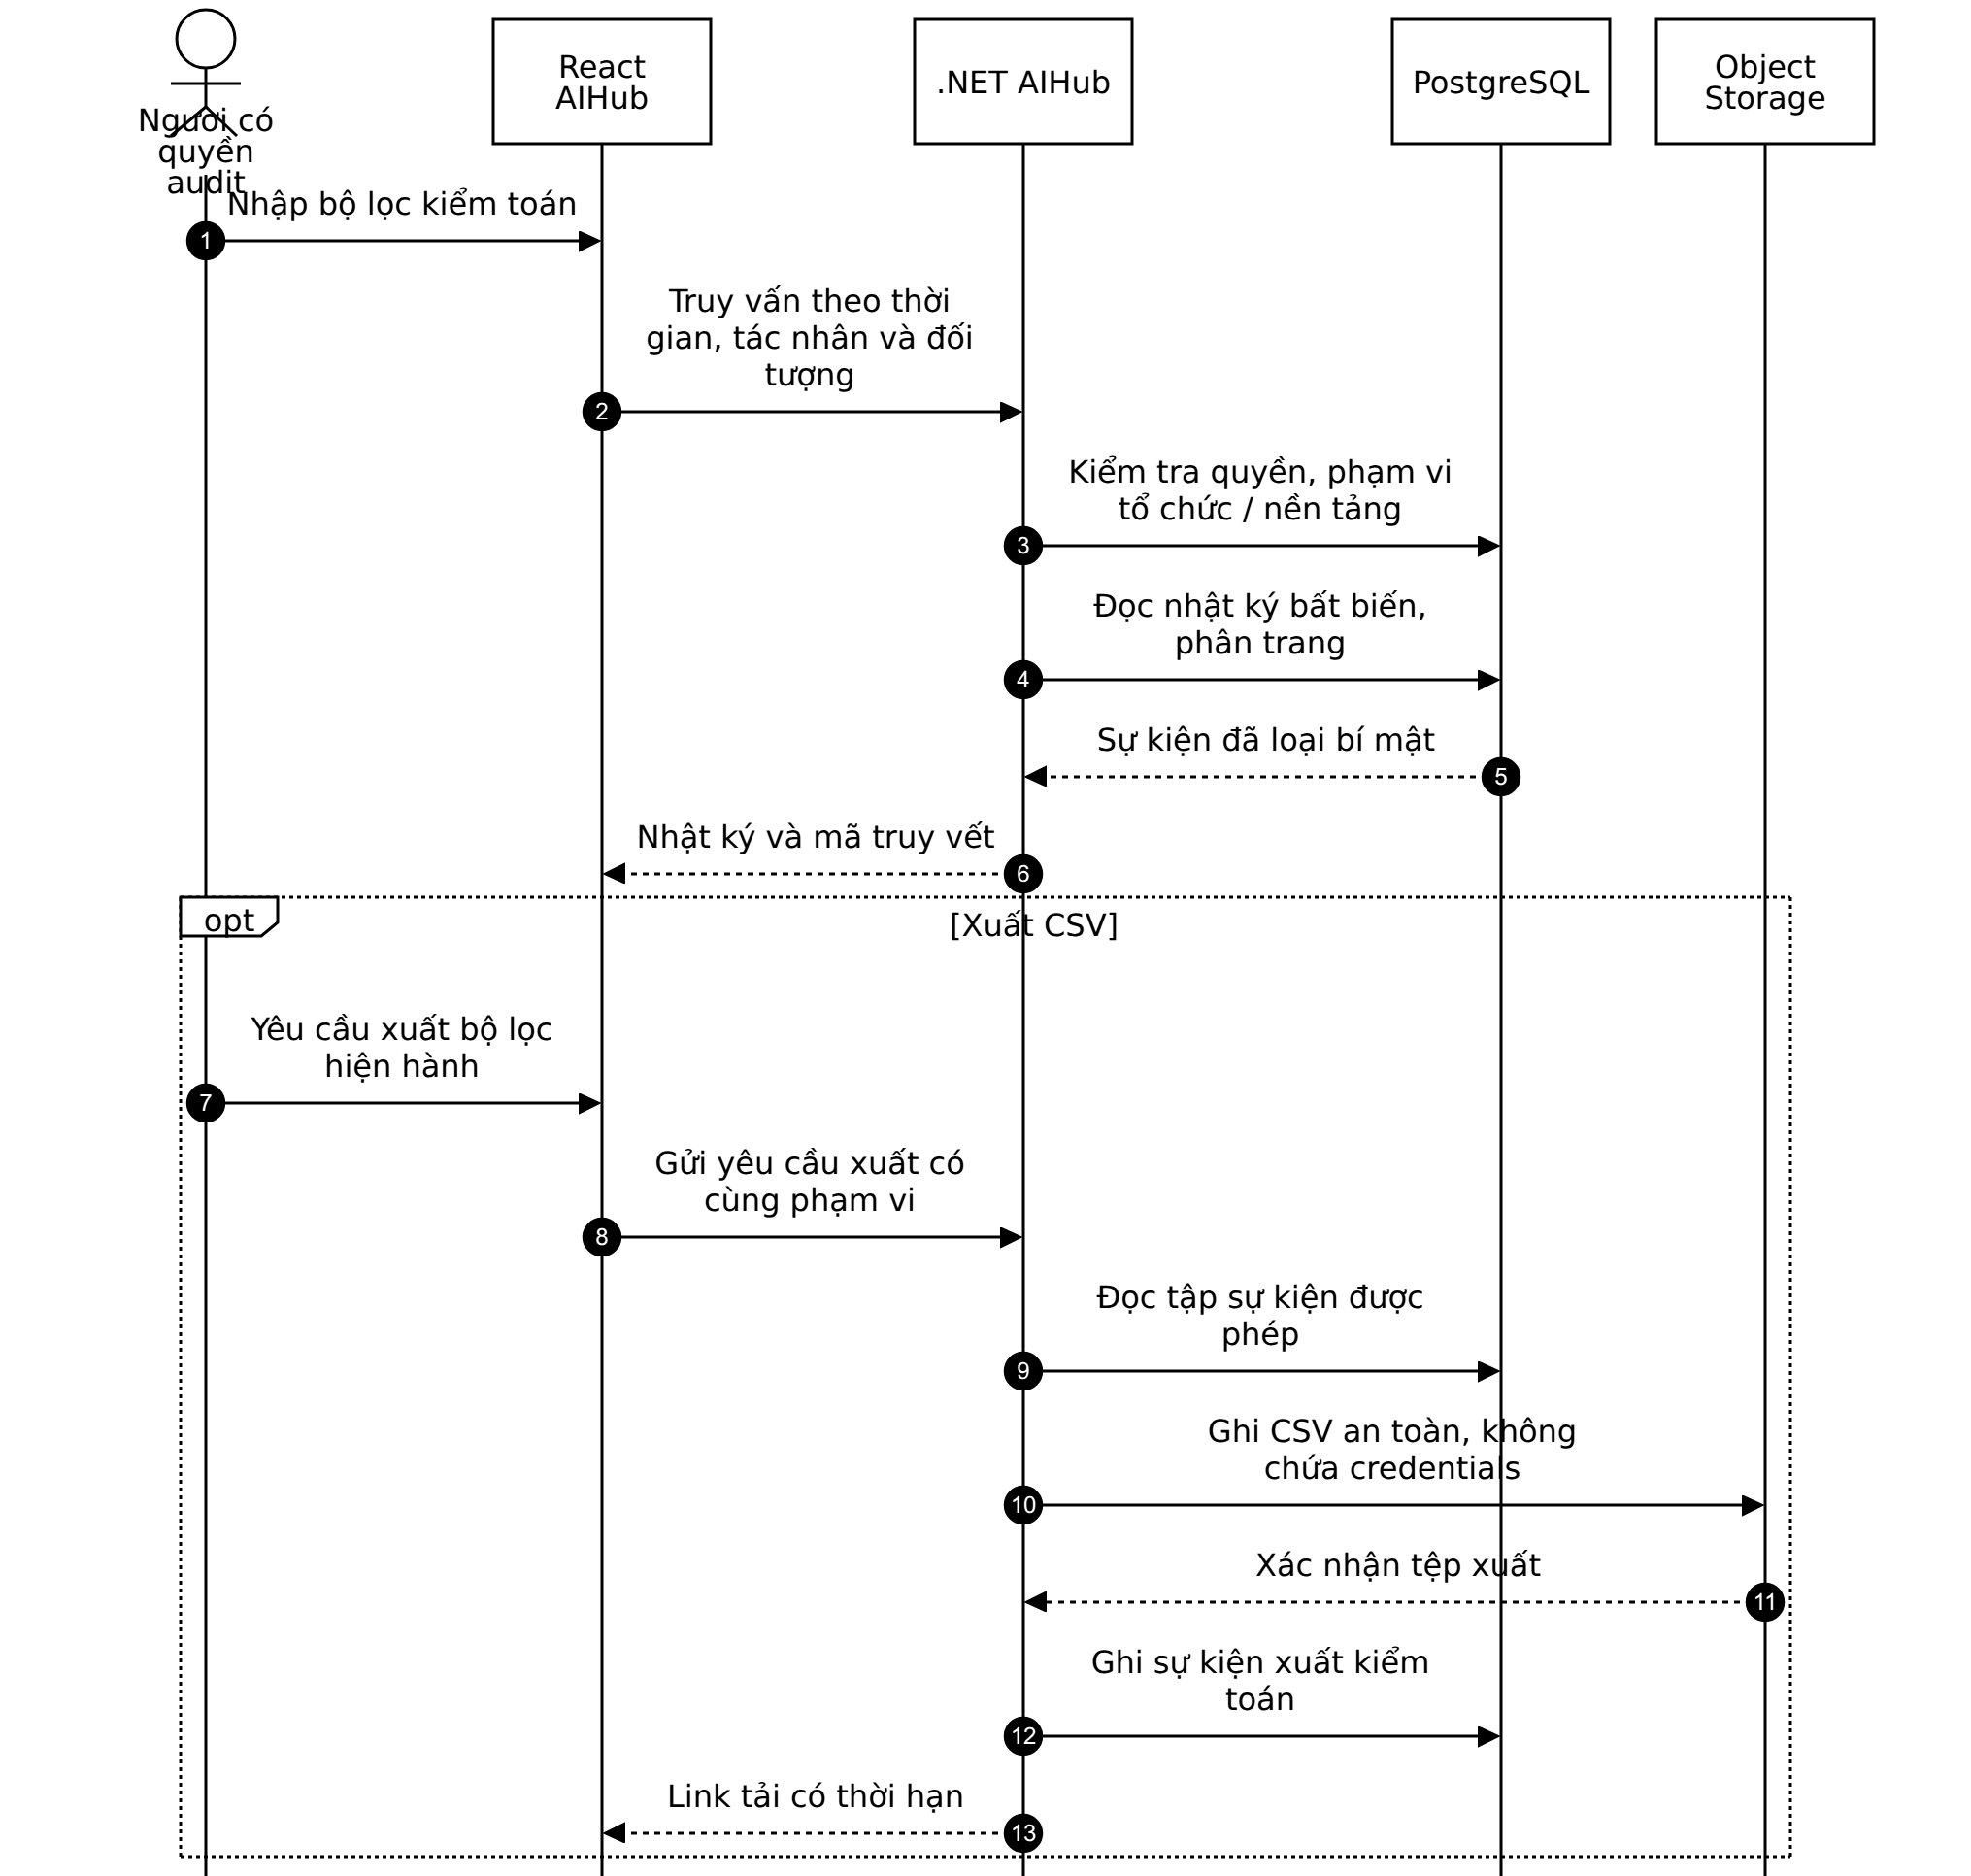
\includegraphics[width=\linewidth,height=.77\textheight,keepaspectratio]{Images/Sequence/AIHub/sequence_uc20_audit_logs.png}
\caption{Sequence diagram AIHub UC20 — Kiểm toán và truy vết giao dịch}
\label{sequence:aihub:sequence_uc20_audit_logs}
\end{figure}

Truy vấn và xuất dữ liệu áp dụng cùng phạm vi quyền; nhật ký không cung cấp thao tác sửa hoặc xóa trên Portal.

\subsubsection{Bảo mật và vận hành riêng của AIHub}

Gateway suy ra tổ chức từ credentials đã xác minh, sau đó kiểm tra quyền dịch vụ, trạng thái khóa và hạn mức. Portal sử dụng phiên người dùng; khóa B2B chỉ được cấp cho ứng dụng máy chủ của đối tác. Khu vực Academic Lab được kiểm tra bằng quyền nội bộ riêng tại từng endpoint.

B2B có hàng đợi \texttt{b2b.\allowbreak{}inference} và Academic Lab có hàng đợi \texttt{lab.\allowbreak{}generation}. Các tác vụ không được sử dụng hết tài nguyên GPU dành cho Wispace. Mọi thao tác cấp/thu hồi khóa, chuyển Owner, sửa gói, override quota, đổi model route và xuất dữ liệu đều cần audit. Khi công bố một dịch vụ, schema, phiên bản và quy tắc tính hạn mức phải được quản lý cùng nhau.

\subsection{Công nghệ, nguyên tắc tích hợp và triển khai}

\subsubsection{Kiến trúc vật lý và công nghệ}

Wispace và AIHub có frontend, backend .NET, Worker và cơ sở dữ liệu riêng. Hai hệ thống có thể áp dụng cùng bộ công nghệ và dùng hạ tầng vật lý chung trong phạm vi đồ án, nhưng được triển khai thành các dịch vụ độc lập. Việc chia sẻ máy chủ không cho phép truy cập chéo dữ liệu, phiên đăng nhập hoặc hạn mức.

\paragraph*{Lựa chọn mô hình kiến trúc}

Wispace được thiết kế theo microservices có chọn lọc: Core, Learning, Assessment, Reporting và AI Inference có khả năng phát hành và mở rộng độc lập. Nội bộ Core được chia module để giữ các nghiệp vụ nền tảng dễ quản lý. AIHub giữ kiến trúc \textbf{modular monolith} với API B2B, Portal và Academic Lab trong backend riêng. Sự khác biệt phản ánh nhu cầu phiên thi và suy luận của Wispace; không bắt buộc hai hệ thống có cùng mô hình triển khai \cite{ch7_microservices}.

Mỗi hệ thống có tiến trình .NET Worker và cấu hình hàng đợi riêng, triển khai từ bộ mã nguồn của backend tương ứng. API host tiếp nhận yêu cầu và tạo công việc; Worker xử lý công việc đã được ghi nhận. Worker là đơn vị triển khai riêng để yêu cầu HTTP có thể kết thúc sau khi nhận bài, còn việc chấm tiếp tục độc lập với kết nối của người dùng.

AI Runtime sử dụng Python FastAPI và được triển khai tách khỏi .NET. Hai hệ thống có thể gọi cùng dịch vụ suy luận đã được cấp quyền, bằng credentials và giới hạn tải riêng; đây là tích hợp dịch vụ AI, không phải dùng chung backend nghiệp vụ. Việc tách này cho phép sử dụng thư viện học máy, quản lý tài nguyên GPU và mở rộng năng lực suy luận theo nhu cầu. Trong từng module .NET, logic nghiệp vụ được tổ chức theo các lớp Domain, Application và Infrastructure; hướng phụ thuộc được quản lý thông qua interface và dependency injection \cite{ch7_dotnet_architecture}.

\begin{figure}[H]
\centering
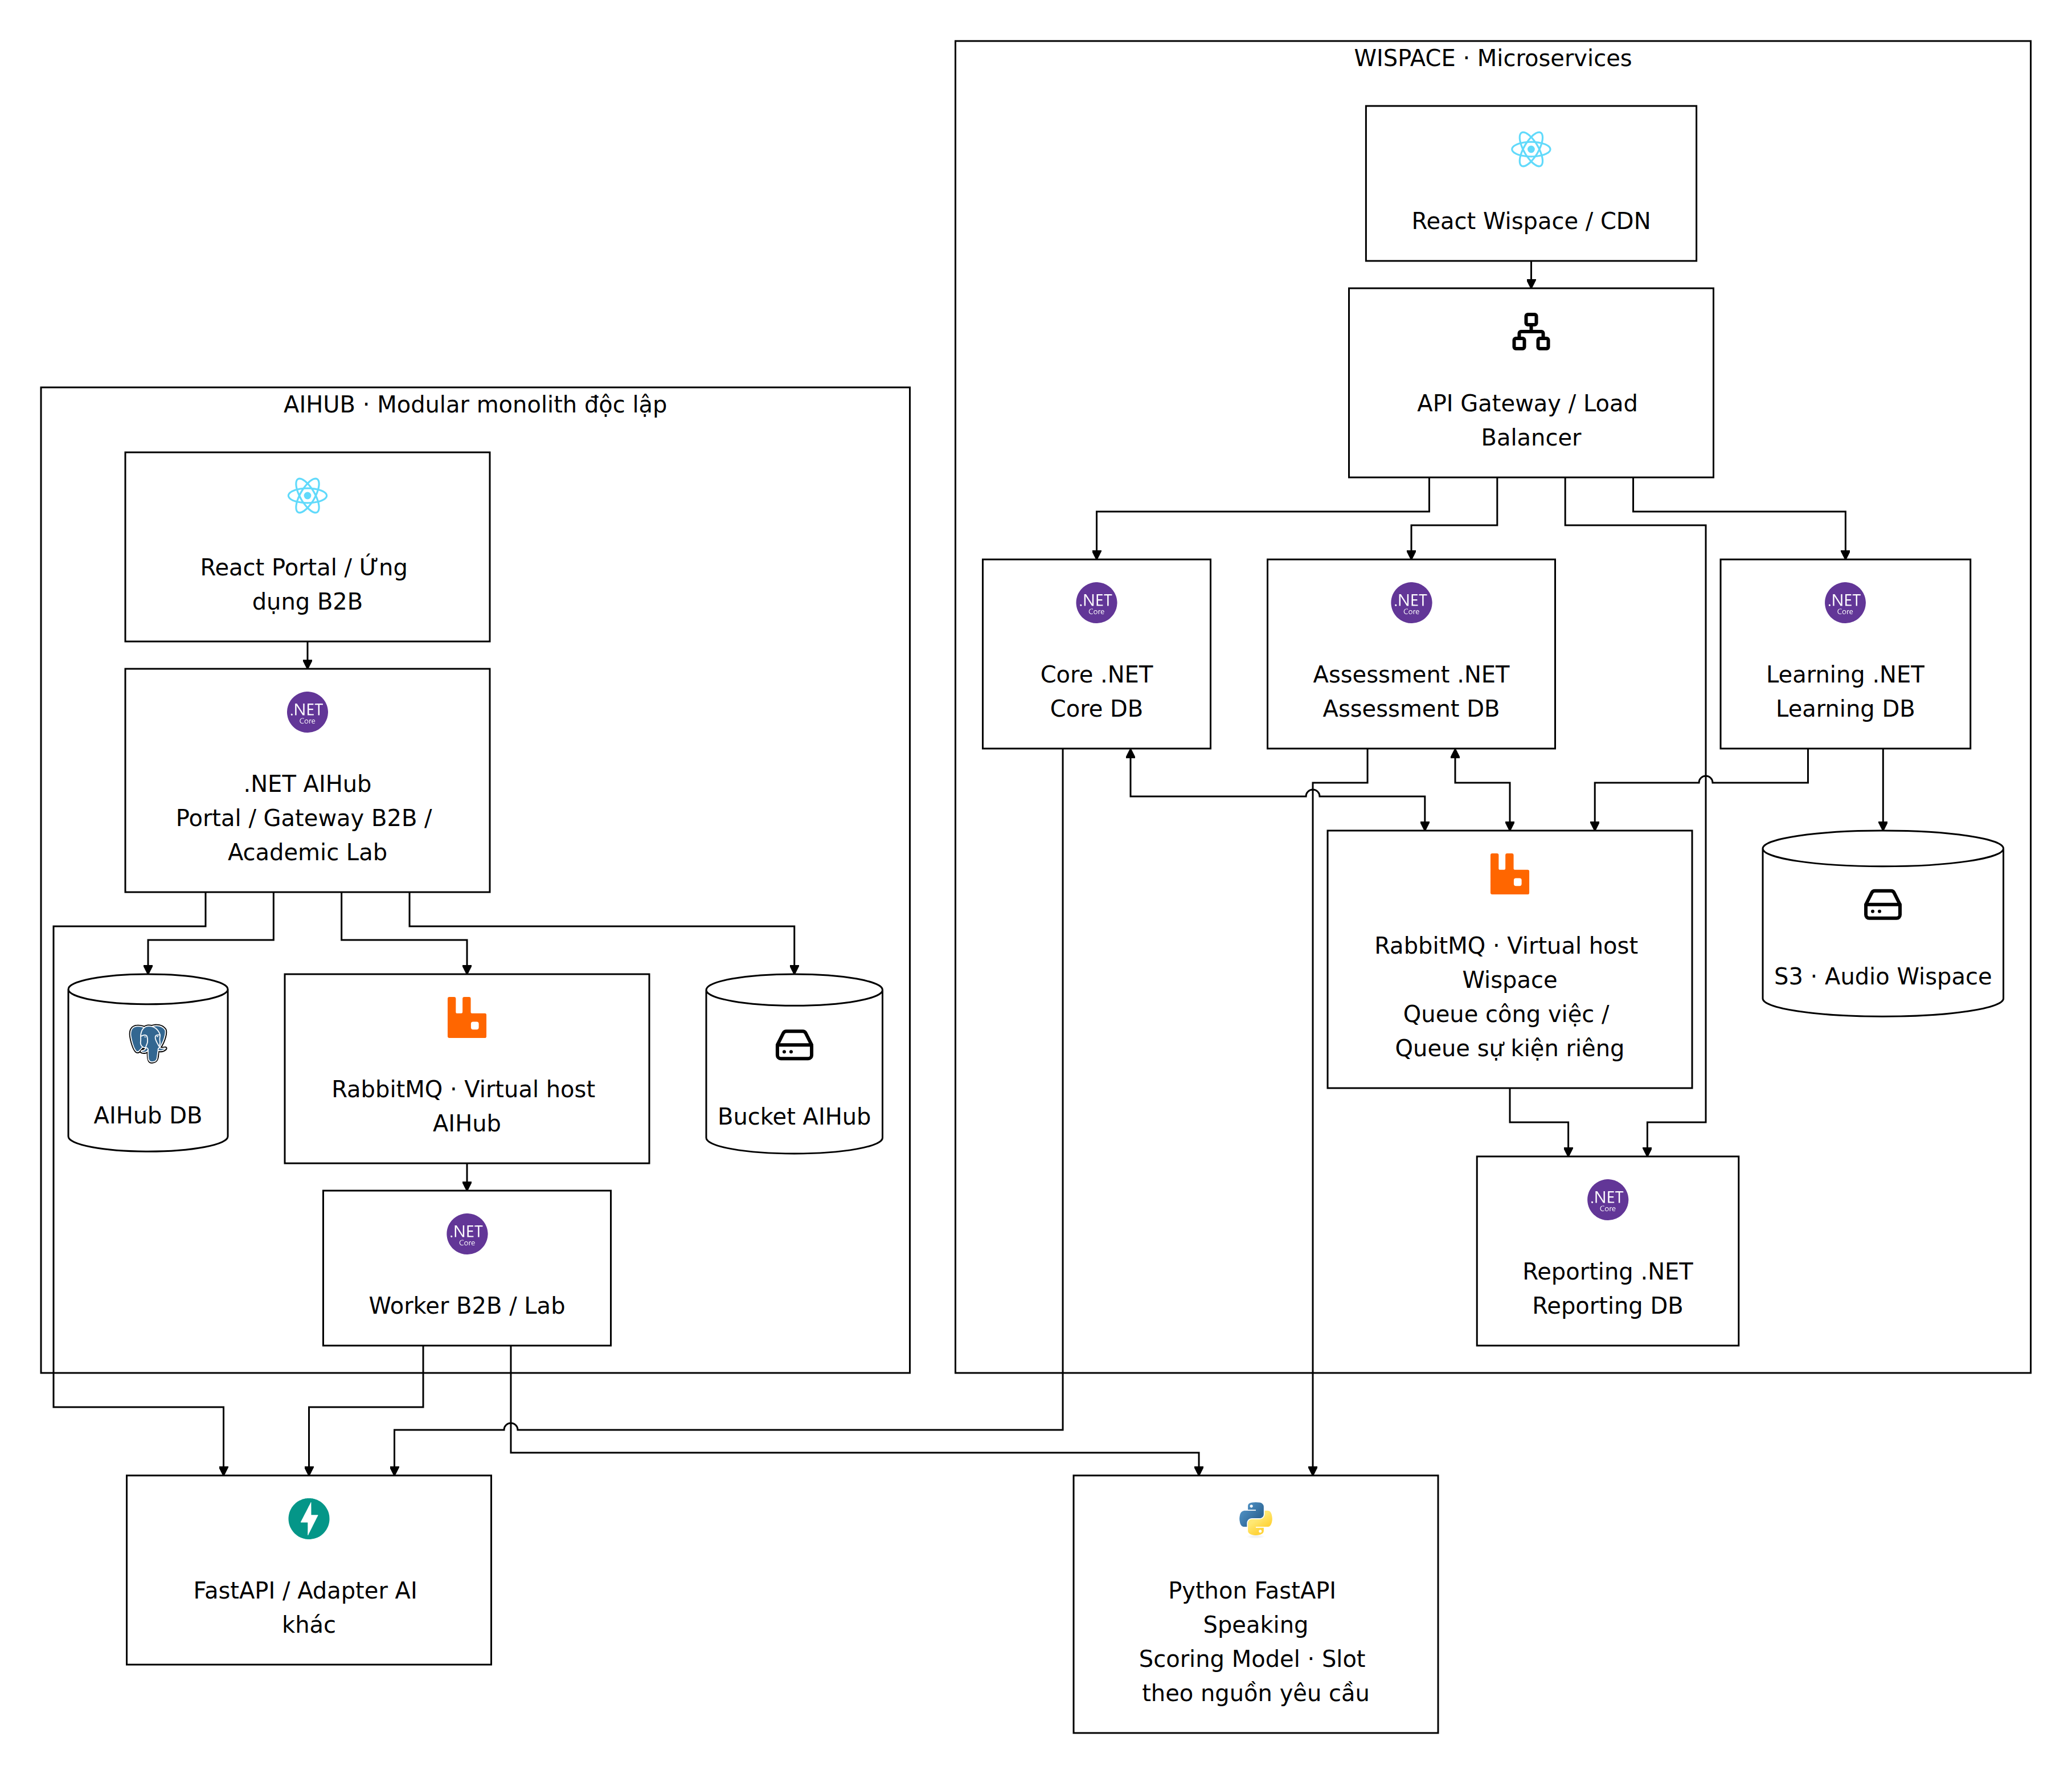
\includegraphics[width=\linewidth,height=.72\textheight,keepaspectratio]{Images/Design/shared_architecture.png}
\caption{Kiến trúc tổng thể hai hệ thống độc lập Wispace và AIHub}
\label{design:fig:shared_architecture}
\end{figure}

Sơ đồ biểu diễn các kênh xử lý chính. Khi Wispace cần tạo TTS hoặc thực hiện một tác vụ AI ngắn, Core hoặc dịch vụ Wispace được cấp quyền có thể gọi adapter FastAPI trực tiếp với timeout phù hợp. Đối với chấm bài và tác vụ dài, lời gọi được thực hiện bởi Worker thuộc luồng xử lý của Wispace. Luồng này không đi qua cổng API B2B của AIHub.

Đối tác chỉ truy cập các endpoint B2B công khai của .NET. FastAPI, RabbitMQ và PostgreSQL nằm trong mạng nội bộ. Frontend có thể truyền tệp trực tiếp đến Object Storage bằng quyền tải lên có thời hạn do backend cấp; các yêu cầu nghiệp vụ vẫn được xử lý qua .NET.

\paragraph*{Công nghệ đề xuất}

\begingroup\small\setstretch{1.1}
\begin{longtable}{|>{\raggedright\arraybackslash}p{\dimexpr 0.21\linewidth-2\tabcolsep-2\arrayrulewidth\relax}|>{\raggedright\arraybackslash}p{\dimexpr 0.35\linewidth-2\tabcolsep-2\arrayrulewidth\relax}|>{\raggedright\arraybackslash}p{\dimexpr 0.44\linewidth-2\tabcolsep-2\arrayrulewidth\relax}|}
\caption{Công nghệ đề xuất}\label{design:tab:3}\\
\hline
\textbf{Nhóm} & \textbf{Công nghệ} & \textbf{Mục đích} \\ \hline
\endfirsthead
\hline
\textbf{Nhóm} & \textbf{Công nghệ} & \textbf{Mục đích} \\ \hline
\endhead
\endfoot
Giao diện & React, TypeScript, Vite, React Router & Hai ứng dụng giao diện riêng; tổ chức route và màn hình theo nghiệp vụ. \\ \hline
Dữ liệu phía trình duyệt & TanStack Query & Quản lý dữ liệu lấy từ API, trạng thái tải và làm mới kết quả. \\ \hline
Backend & ASP.NET Core Web API & Cung cấp API, xác thực, phân quyền và xử lý nghiệp vụ theo module. \\ \hline
Truy cập dữ liệu & EF Core và Npgsql & Ánh xạ dữ liệu và thực hiện giao dịch trên PostgreSQL \cite{ch7_npgsql}. \\ \hline
Cơ sở dữ liệu & PostgreSQL & Nguồn dữ liệu chính cho tài khoản, bài làm, kết quả, hạn mức và cấu hình. \\ \hline
Tác vụ nền & .NET Worker / BackgroundService & Tiêu thụ công việc, gọi FastAPI và cập nhật kết quả. \\ \hline
Hàng đợi & RabbitMQ & Chuyển công việc giữa API host và Worker; xác nhận phát và xử lý thông điệp. \\ \hline
Lưu trữ tệp & Object Storage tương thích S3 & Lưu audio, tệp dữ liệu xuất và các tài nguyên mô hình ở vùng lưu trữ phù hợp. \\ \hline
AI & Python FastAPI và thư viện suy luận của Scoring Model & Đóng gói API suy luận, tiền xử lý âm thanh và các adapter AI. \\ \hline
Thông báo thời gian thực & ASP.NET Core SignalR & Thông báo tiến trình và kết quả; REST API vẫn cung cấp trạng thái có thể truy vấn lại. \\ \hline
Bộ nhớ đệm, khi cần mở rộng & Redis & Cache danh mục, cấu hình và trạng thái ngắn hạn; không thay thế dữ liệu nghiệp vụ trong PostgreSQL. \\ \hline
Triển khai & Docker Compose, reverse proxy Nginx & Đóng gói các thành phần và triển khai mô hình thử nghiệm của đồ án. \\ \hline
\end{longtable}
\endgroup

Phiên bản .NET, EF Core và Npgsql được chọn đồng bộ khi hiện thực. Các dependency React và Python được cố định bằng lockfile hoặc danh sách phiên bản để tái lập môi trường. Redis là thành phần mở rộng; bản triển khai ban đầu có thể sử dụng PostgreSQL cho các kiểm tra hạn mức và trạng thái để giảm số dịch vụ cần vận hành.

\subsubsection{Tổ chức lớp và giao dịch liên module}

Mỗi module chứa bốn nhóm thành phần:

\begin{itemize}
\item \textbf{API:} controller, xác thực request, DTO và ánh xạ lỗi HTTP.
\item \textbf{Application:} thực hiện ca sử dụng, kiểm tra quyền nghiệp vụ, điều phối giao dịch và gọi các interface tích hợp.
\item \textbf{Domain:} thực thể, trạng thái và các quy tắc như điều kiện nộp bài, quyền lợi gói hoặc vòng đời credentials.
\item \textbf{Infrastructure:} EF Core, PostgreSQL, RabbitMQ, Object Storage và HTTP client gọi FastAPI hoặc dịch vụ ngoài.
\end{itemize}

Domain không phụ thuộc trực tiếp EF Core hoặc SDK của nhà cung cấp AI. Các interface như \texttt{ISpeaking\allowbreak{}Scoring\allowbreak{}Client}, \texttt{IObject\allowbreak{}Storage}, \texttt{IQuota\allowbreak{}Service} và \texttt{IModel\allowbreak{}Provider} giúp thay thế cách tích hợp mà không thay đổi quy tắc nghiệp vụ.

\begin{figure}[H]
\centering
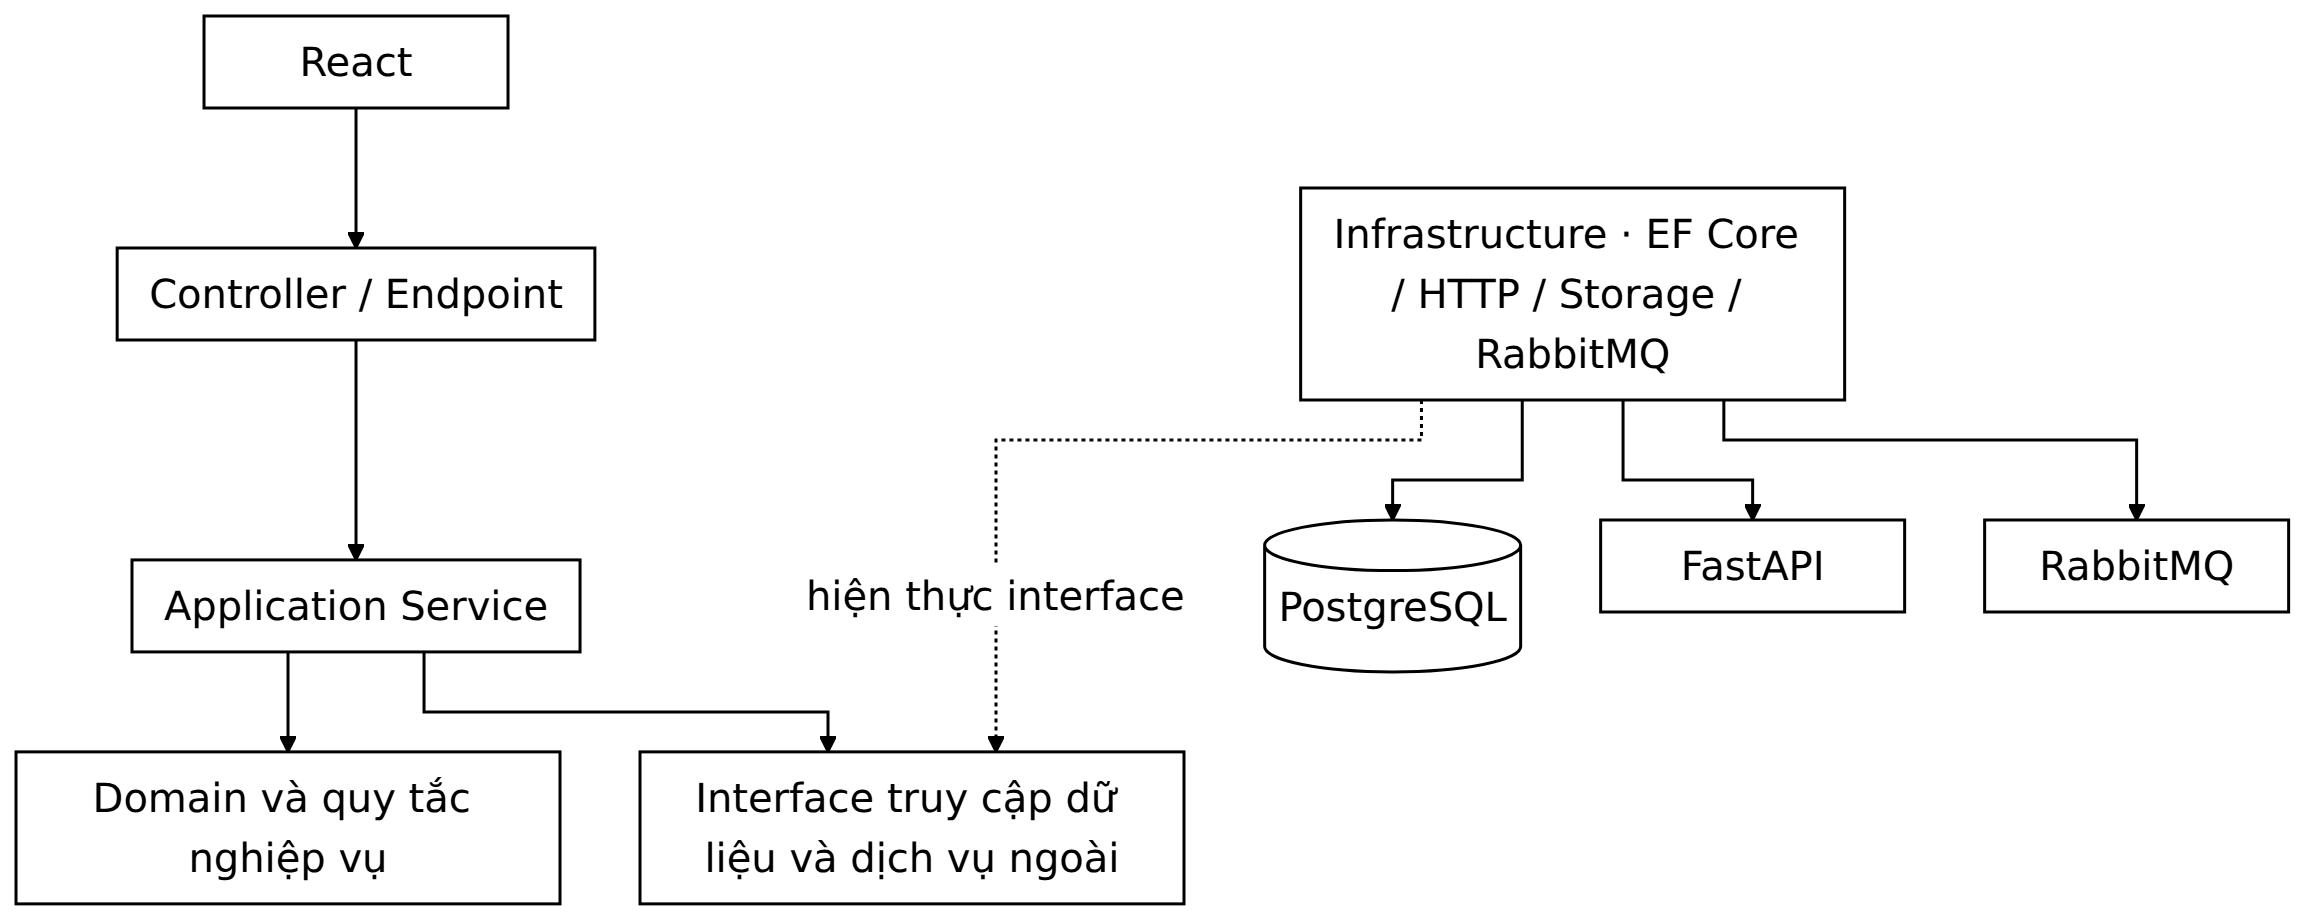
\includegraphics[width=\linewidth,height=.72\textheight,keepaspectratio]{Images/Design/module_layers.png}
\caption{Các lớp xử lý trong module .NET}
\label{design:fig:module_layers}
\end{figure}

Các mũi tên nét đứt trong sơ đồ biểu diễn quan hệ hiện thực interface. Ứng dụng kết nối các hiện thực cụ thể thông qua dependency injection khi khởi động.

Wispace dùng Core DB, Learning DB, Assessment DB và Reporting DB với quyền ghi và migration riêng. Core không sửa trực tiếp trạng thái job; Assessment không cập nhật sổ quota; Reporting không sửa dữ liệu nguồn. API đồng bộ được dùng cho truy vấn cần phản hồi ngay và giữ quyền lợi; sự kiện bất đồng bộ truyền kết quả và đồng bộ projection. Không duy trì transaction PostgreSQL hoặc khóa phân tán xuyên các dịch vụ trong lúc gọi mạng.

Trong Core, tài khoản/gói/quota có thể dùng transaction cục bộ qua hợp đồng module; trong AIHub, giao dịch B2B vẫn có thể dùng cùng connection của AIHub DB. Không áp dụng giả định transaction liên module này cho Learning, Core và Assessment đã tách biệt. Thay đổi hợp đồng cần tương thích phiên bản trong thời gian triển khai cuốn chiếu.

\subsubsection{Danh mục dữ liệu và ràng buộc nhất quán}

Bảng dưới đây mô tả các nhóm bảng, không phải một database dùng chung. Nhóm identity, question và billing của Wispace thuộc Core DB; session, answer và audio thuộc Learning DB; job, attempt, result và share thuộc Assessment DB; trend và roadmap thuộc Reporting DB. Mỗi dịch vụ có outbox/inbox và audit riêng. AIHub DB sở hữu identity của AIHub, aihub và lab; tên schema trùng nhau giữa các database không đồng nghĩa dùng chung danh tính.

\begingroup\small\setstretch{1.1}
\begin{longtable}{|>{\raggedright\arraybackslash}p{\dimexpr 0.13\linewidth-2\tabcolsep-2\arrayrulewidth\relax}|>{\raggedright\arraybackslash}p{\dimexpr 0.49\linewidth-2\tabcolsep-2\arrayrulewidth\relax}|>{\raggedright\arraybackslash}p{\dimexpr 0.38\linewidth-2\tabcolsep-2\arrayrulewidth\relax}|}
\caption{Danh mục dữ liệu và ràng buộc nhất quán}\label{design:tab:4}\\
\hline
\textbf{Schema} & \textbf{Nhóm bảng đề xuất} & \textbf{Nội dung chính} \\ \hline
\endfirsthead
\hline
\textbf{Schema} & \textbf{Nhóm bảng đề xuất} & \textbf{Nội dung chính} \\ \hline
\endhead
\endfoot
\texttt{identity} & \texttt{users}, \texttt{roles}, \texttt{user\_\allowbreak{}roles}, \texttt{sessions}, \texttt{refresh\_\allowbreak{}tokens}, \texttt{verification\_\allowbreak{}codes}, \texttt{consents} & Danh tính, phiên, xác minh và các lần đồng ý xử lý/sử dụng dữ liệu. \\ \hline
\texttt{core} & \texttt{question\_\allowbreak{}sets}, \texttt{questions}, \texttt{question\_\allowbreak{}audio}, \texttt{question\_\allowbreak{}submissions}, \texttt{question\_\allowbreak{}reports} & Kho đề và quy trình kiểm duyệt. \\ \hline
\texttt{learn\allowbreak{}ing} & \texttt{learning\_\allowbreak{}sessions}, \texttt{answers}, \texttt{audio\_\allowbreak{}assets} & Phiên học, câu trả lời, manifest audio và submission; job và attempt thuộc Assessment DB. \\ \hline
\texttt{assess\allowbreak{}ment} & \texttt{assessment\_\allowbreak{}results}, \texttt{criterion\_\allowbreak{}scores}, \texttt{detected\_\allowbreak{}errors}, \texttt{assessment\_\allowbreak{}jobs}, \texttt{assessment\_\allowbreak{}attempts}, \texttt{share\_\allowbreak{}links} & Job, attempt, kết quả, lỗi, báo cáo thi thử và link chia sẻ. \\ \hline
\texttt{report\allowbreak{}ing} & \texttt{progress\_projections}, \texttt{roadmap\_items}, \texttt{inbox\_events} & Tổng hợp lịch sử, xu hướng và roadmap từ sự kiện. \\ \hline
\texttt{billing} & \texttt{plans}, \texttt{plan\_\allowbreak{}entitlements}, \texttt{subscriptions}, \texttt{quota\_\allowbreak{}accounts}, \texttt{quota\_\allowbreak{}reservations}, \texttt{quota\_\allowbreak{}entries} & Gói Self-practice và sổ sử dụng hạn mức của học viên. \\ \hline
\texttt{billing} & \texttt{payment\_\allowbreak{}orders}, \texttt{payment\_\allowbreak{}events} & Đơn và thông báo thanh toán PayOS. \\ \hline
\texttt{aihub} & \texttt{organizations}, \texttt{organization\_\allowbreak{}members}, \texttt{api\_\allowbreak{}credentials}, \texttt{service\_\allowbreak{}catalog}, \texttt{model\_\allowbreak{}routes} & Khách hàng B2B, khóa và danh mục dịch vụ. \\ \hline
\texttt{aihub} & \texttt{organization\_\allowbreak{}plans}, \texttt{organization\_\allowbreak{}quota\_\allowbreak{}accounts}, \texttt{organization\_\allowbreak{}quota\_\allowbreak{}reservations}, \texttt{api\_\allowbreak{}requests}, \texttt{usage\_\allowbreak{}events} & Hạn mức và dữ liệu thực thi API của từng tổ chức. \\ \hline
\texttt{lab} & \texttt{references}, \texttt{samples}, \texttt{sample\_\allowbreak{}reviews}, \texttt{prompt\_\allowbreak{}versions}, \texttt{dataset\_\allowbreak{}exports}, \texttt{dataset\_\allowbreak{}export\_\allowbreak{}items} & Dẫn chứng, mẫu học thuật, thẩm định và xuất dữ liệu nội bộ. \\ \hline
\texttt{platform} & \texttt{model\_\allowbreak{}versions}, \texttt{file\_\allowbreak{}assets}, \texttt{outbox\_\allowbreak{}messages}, \texttt{audit\_\allowbreak{}events} & Phiên bản mô hình, tệp, sự kiện tích hợp và kiểm toán. \\ \hline
\end{longtable}
\endgroup

Các tên bảng là đề xuất phục vụ thiết kế. Hệ thống dùng khóa chính UUID cho các đối tượng có thể được truy cập qua API. Các thời điểm được lưu theo UTC; giao diện chuyển đổi theo múi giờ của người dùng. Dữ liệu có cấu trúc ổn định như điểm, trạng thái, chủ sở hữu và khóa ngoại được lưu bằng cột quan hệ. Metadata mở rộng của phản hồi AI có thể lưu bằng \texttt{jsonb} kèm phiên bản schema.

\begin{itemize}
\item Mỗi công việc chấm được định danh độc lập với từng lần thử. Kết quả cuối cùng có ràng buộc duy nhất theo \texttt{assessment\allowbreak{}Job\allowbreak{}Id}.
\item Một yêu cầu nộp có \texttt{Idempotency-\allowbreak{}Key} được ràng buộc theo người dùng, loại thao tác và mã yêu cầu; gửi lại cùng khóa không tạo thêm lượt chấm hoặc bút toán quota.
\item Sổ hạn mức có định danh nghiệp vụ duy nhất cho từng hành động giữ, tiêu thụ và hoàn. Số dư được kiểm tra và cập nhật trong transaction có khóa hoặc cập nhật có điều kiện.
\item Một thông báo PayOS được lưu với mã sự kiện duy nhất. Nhận lại cùng một thông báo không kích hoạt thêm thuê bao.
\item Các bản hiệu đính của Academic Lab sử dụng số phiên bản để phát hiện cập nhật đồng thời. \texttt{raw\allowbreak{}Ai\allowbreak{}Output} của mẫu gốc được bảo toàn.
\item Các bảng tổ chức B2B có \texttt{organization\allowbreak{}Id} và chỉ mục phục vụ lọc theo tổ chức. Những quan hệ cần cùng tenant được ràng buộc bằng khóa hoặc kiểm tra giao dịch tương ứng.
\end{itemize}

\subsubsection{Hợp đồng API và cập nhật trạng thái}

\paragraph*{Nhóm endpoint đề xuất}

\begingroup\small\setstretch{1.1}
\begin{longtable}{|>{\raggedright\arraybackslash}p{\dimexpr 0.21\linewidth-2\tabcolsep-2\arrayrulewidth\relax}|>{\raggedright\arraybackslash}p{\dimexpr 0.35\linewidth-2\tabcolsep-2\arrayrulewidth\relax}|>{\raggedright\arraybackslash}p{\dimexpr 0.44\linewidth-2\tabcolsep-2\arrayrulewidth\relax}|}
\caption{Nhóm endpoint đề xuất}\label{design:tab:5}\\
\hline
\textbf{Nhóm} & \textbf{Ví dụ endpoint} & \textbf{Trách nhiệm} \\ \hline
\endfirsthead
\hline
\textbf{Nhóm} & \textbf{Ví dụ endpoint} & \textbf{Trách nhiệm} \\ \hline
\endhead
\endfoot
Identity & \texttt{POST /\allowbreak{}api/\allowbreak{}v1/\allowbreak{}auth/\allowbreak{}login}, \texttt{POST /\allowbreak{}api/\allowbreak{}v1/\allowbreak{}auth/\allowbreak{}refresh} & Xác thực tài khoản và gia hạn phiên trình duyệt. \\ \hline
Kho đề Wispace & \texttt{GET /\allowbreak{}api/\allowbreak{}v1/\allowbreak{}wispace/\allowbreak{}questions} & Truy vấn đề theo quyền xem và bộ lọc. \\ \hline
Audio Wispace & \texttt{POST /\allowbreak{}api/\allowbreak{}v1/\allowbreak{}wispace/\allowbreak{}answers/\allowbreak{}\{id\}/\allowbreak{}uploads} & Tạo phiên tải audio và cấp quyền tải lên. \\ \hline
Hoàn tất audio & \texttt{POST /\allowbreak{}api/\allowbreak{}v1/\allowbreak{}wispace/\allowbreak{}uploads/\allowbreak{}\{id\}/\allowbreak{}complete} & Xác minh tệp hoặc các đoạn đã tải. \\ \hline
Nộp bài chấm & \texttt{POST /\allowbreak{}api/\allowbreak{}v1/\allowbreak{}wispace/\allowbreak{}answers/\allowbreak{}\{id\}/\allowbreak{}assessments} & Learning điều phối giữ quota tại Core, nhận submission và trả \texttt{202}; Assessment tạo job từ sự kiện. \\ \hline
Trạng thái nộp & \texttt{GET /\allowbreak{}api/\allowbreak{}v1/\allowbreak{}wispace/\allowbreak{}submissions/\allowbreak{}\{id\}} & Learning trả trạng thái tiếp nhận và các jobId đã được Assessment xác nhận; client chưa cần biết jobId khi nhận HTTP 202. \\ \hline
Kết quả & \texttt{GET /\allowbreak{}api/\allowbreak{}v1/\allowbreak{}wispace/\allowbreak{}assessments/\allowbreak{}\{id\}} & Trạng thái hoặc báo cáo theo quyền sở hữu. \\ \hline
Portal AIHub & \texttt{POST /\allowbreak{}api/\allowbreak{}v1/\allowbreak{}aihub/\allowbreak{}organizations/\allowbreak{}\{id\}/\allowbreak{}credentials} & Quản lý credentials theo quyền trong tổ chức. \\ \hline
API B2B & \texttt{POST /\allowbreak{}b2b/\allowbreak{}v1/\allowbreak{}services/\allowbreak{}\{service\allowbreak{}Code\}/\allowbreak{}requests} & Tiếp nhận yêu cầu đối tác và chọn cơ chế thực thi. \\ \hline
Trạng thái B2B & \texttt{GET /\allowbreak{}b2b/\allowbreak{}v1/\allowbreak{}requests/\allowbreak{}\{request\allowbreak{}Id\}} & Truy vấn yêu cầu thuộc tổ chức đã xác thực. \\ \hline
Academic Lab & \texttt{POST /\allowbreak{}api/\allowbreak{}v1/\allowbreak{}internal/\allowbreak{}lab/\allowbreak{}samples/\allowbreak{}\{id\}/\allowbreak{}reviews} & Ghi quyết định thẩm định của nhân sự nội bộ. \\ \hline
PayOS webhook & \texttt{POST /\allowbreak{}api/\allowbreak{}v1/\allowbreak{}payments/\allowbreak{}payos/\allowbreak{}webhook} & Xác minh thông báo thanh toán và cập nhật giao dịch. \\ \hline
AI nội bộ & \texttt{POST /\allowbreak{}internal/\allowbreak{}v1/\allowbreak{}speaking/\allowbreak{}assessments} & FastAPI thực thi một yêu cầu suy luận Speaking. \\ \hline
\end{longtable}
\endgroup

Các endpoint là hợp đồng đề xuất. API public của .NET, API B2B và API nội bộ của FastAPI được version hóa độc lập. Thay đổi schema không tương thích cần có phiên bản mới hoặc adapter chuyển đổi; không thay đổi ngầm phản hồi mà client đang sử dụng.

\paragraph*{Phản hồi và lỗi}

Lỗi trả về gồm mã lỗi nghiệp vụ, thông báo có thể hiển thị, \texttt{trace\allowbreak{}Id} và các trường không hợp lệ khi phù hợp. Không đưa stack trace, connection string, khóa bí mật hoặc URL audio riêng tư vào phản hồi lỗi.

Các mã HTTP được sử dụng nhất quán: \texttt{400} cho dữ liệu không hợp lệ, \texttt{401} cho thiếu hoặc sai xác thực, \texttt{403} cho thiếu quyền, \texttt{409} cho xung đột trạng thái hoặc idempotency, \texttt{429} cho giới hạn sử dụng và \texttt{503} khi dịch vụ tạm thời không sẵn sàng. Yêu cầu dài đã được chấp nhận trả \texttt{202}; mã này không biểu thị rằng việc chấm đã hoàn tất.

SignalR gửi các sự kiện như \texttt{Assessment\allowbreak{}Queued}, \texttt{Assessment\allowbreak{}Started}, \texttt{Assessment\allowbreak{}Completed} và \texttt{Assessment\allowbreak{}Failed} đến nhóm kết nối của đúng người dùng. Backend kiểm tra quyền khi đăng ký nhóm nhận thông báo. Thông báo chỉ chứa định danh và trạng thái cần thiết; frontend truy vấn REST API để lấy báo cáo đầy đủ.

Nếu mất kết nối SignalR, frontend tiếp tục truy vấn trạng thái theo chu kỳ với khoảng chờ tăng dần. Sau khi tải lại trang, trạng thái được khôi phục từ PostgreSQL thông qua API, thay vì dựa vào các thông báo đã nhận trước đó.

\subsubsection{Thiết kế bảo mật và quyền riêng tư}

\paragraph*{Tài khoản và phiên trình duyệt}

Backend sử dụng ASP.NET Core Identity cho tài khoản và các chức năng xác thực nền tảng \cite{ch7_aspnet_identity}. Đề xuất thống nhất hai frontend dùng access token thời hạn ngắn và refresh token trong cookie \texttt{Http\allowbreak{}Only}, \texttt{Secure}, với chính sách \texttt{Same\allowbreak{}Site} phù hợp cấu hình tên miền. Access token được giữ trong bộ nhớ của ứng dụng trình duyệt; refresh token được lưu dạng băm trên máy chủ, xoay vòng sau khi dùng và liên kết với phiên thiết bị.

Các endpoint dùng cookie, đặc biệt refresh và logout, phải có biện pháp chống CSRF, kiểm tra nguồn yêu cầu và cấu hình CORS theo đúng origin được phép. Tác vụ đăng xuất hoặc khóa tài khoản cập nhật trạng thái phiên trên máy chủ. API được bảo vệ kiểm tra trạng thái phiên và trạng thái tài khoản theo chính sách để việc thu hồi không chỉ phụ thuộc vào thời điểm JWT hết hạn.

Hai hệ thống quản lý danh tính, phiên đăng nhập và khóa xác thực độc lập. Cookie và token được giới hạn theo ứng dụng, issuer và audience; token Wispace không được chấp nhận tại AIHub. Quyền tổ chức B2B và quyền Academic Lab được kiểm tra trong backend AIHub. Thiết kế này chưa đặt yêu cầu đăng nhập một lần giữa hai hệ thống.

\paragraph*{Quyền sở hữu và phân tách dữ liệu}

Wispace kiểm tra \texttt{owner\allowbreak{}User\allowbreak{}Id} khi truy cập bài làm, audio và báo cáo riêng tư. Liên kết chia sẻ có mã ngẫu nhiên, phạm vi dữ liệu giới hạn và khả năng thu hồi; chỉ cho xem điểm và nhận xét theo yêu cầu, không tự cấp quyền nghe audio.

AIHub kiểm tra tư cách thành viên, vai trò và \texttt{organization\allowbreak{}Id} tại từng thao tác. Mã tổ chức trong URL phải khớp với phạm vi quyền đang có. Chỉ mục và các ràng buộc dữ liệu được thiết kế để tránh liên kết nhầm tài nguyên giữa hai tổ chức.

Các thao tác khóa tài khoản, đổi vai trò, cấp quota, thu hồi credentials, chuyển quyền tổ chức và xuất dữ liệu nội bộ đều ghi nhận kiểm toán. Audit event gồm tác nhân, phạm vi, loại thao tác, thời điểm, định danh đối tượng và lý do khi nghiệp vụ yêu cầu.

\paragraph*{Giao tiếp nội bộ và bảo vệ dữ liệu}

API nội bộ FastAPI chỉ được công bố trong mạng dịch vụ hoặc qua kết nối riêng có xác thực. Worker và các adapter .NET sử dụng service identity hoặc bí mật nội bộ được quản lý theo môi trường. Không dùng khóa B2B của khách hàng làm bí mật kết nối đến AI Runtime.

Backend kiểm tra định dạng, kích thước và quyền đối với audio trước khi xử lý. Nếu hỗ trợ URL đầu vào từ đối tác, hệ thống cần cơ chế nhập tệp có kiểm soát và giới hạn đích truy cập; bản đầu của đồ án nên ưu tiên upload qua quyền do backend cấp để tránh gọi tùy ý tới tài nguyên mạng nội bộ.

Nội dung đề và mẫu học thuật được xem là dữ liệu đầu vào của mô hình. Prompt hệ thống và quy tắc gọi dịch vụ do backend quản lý; văn bản do người dùng gửi không được dùng để thay đổi cấu hình nhà cung cấp hoặc trao quyền công cụ.

\paragraph*{Đồng ý sử dụng dữ liệu và chính sách xóa}

Hệ thống lưu riêng sự đồng ý xử lý audio để cung cấp dịch vụ và sự đồng ý sử dụng dữ liệu để huấn luyện. Việc chấp thuận điều khoản luyện tập không tự động được xem là chấp thuận huấn luyện. Khi xây dựng tập dữ liệu, bộ lọc xuất phải kiểm tra trạng thái đồng ý và các điều kiện sử dụng của từng mẫu.

Audio gốc, transcript, nhãn chuyên gia và dữ liệu dự đoán được phân biệt bằng nguồn gốc và phiên bản. Tập kiểm tra chuẩn được quản lý riêng để tránh sử dụng lại làm dữ liệu huấn luyện. Yêu cầu xóa tài khoản và dữ liệu được triển khai bằng quy trình có trạng thái, nhật ký và khả năng thử lại khi một hệ lưu trữ tạm thời gặp lỗi.

\subsubsection{Thiết kế triển khai và tài nguyên}

\paragraph*{Mô hình triển khai đề xuất}

Môi trường đồ án sử dụng Docker Compose cho các thành phần ứng dụng và dữ liệu. Hai frontend được build thành tài nguyên tĩnh, phục vụ qua reverse proxy. Wispace triển khai Core API, Learning API, Assessment API/Worker và Reporting API/Worker bằng các image riêng; FastAPI chạy trên nhóm máy GPU. AIHub API/Worker có image và lịch phát hành riêng. PostgreSQL có thể cùng cụm vật lý nhưng database và quyền truy cập tách theo dịch vụ; RabbitMQ dùng virtual host và credentials riêng cho Wispace/AIHub, với quyền exchange/queue phù hợp mỗi dịch vụ; Object Storage tách bucket và quyền theo nguồn dữ liệu. Docker Compose phục vụ phát triển và kiểm thử; production sử dụng nền tảng điều phối container nhiều máy hoặc cơ chế tương đương có health check, cân bằng tải, giới hạn tài nguyên và rolling deployment. Một máy chạy Compose không được xem là kiến trúc đáp ứng sẵn sàng cao cho tải mục tiêu.

Scoring Model được triển khai trên máy có GPU phù hợp; API host và PostgreSQL không phụ thuộc việc chạy chung máy GPU. Các dịch vụ AI khác có thể chạy trên CPU hoặc sử dụng nhà cung cấp ngoài tùy loại tác vụ. Docker Compose có thể tổ chức trên từng máy; việc kết nối máy GPU ở vị trí khác phải dùng mạng riêng hoặc kênh kết nối được bảo vệ.

\begin{figure}[H]
\centering
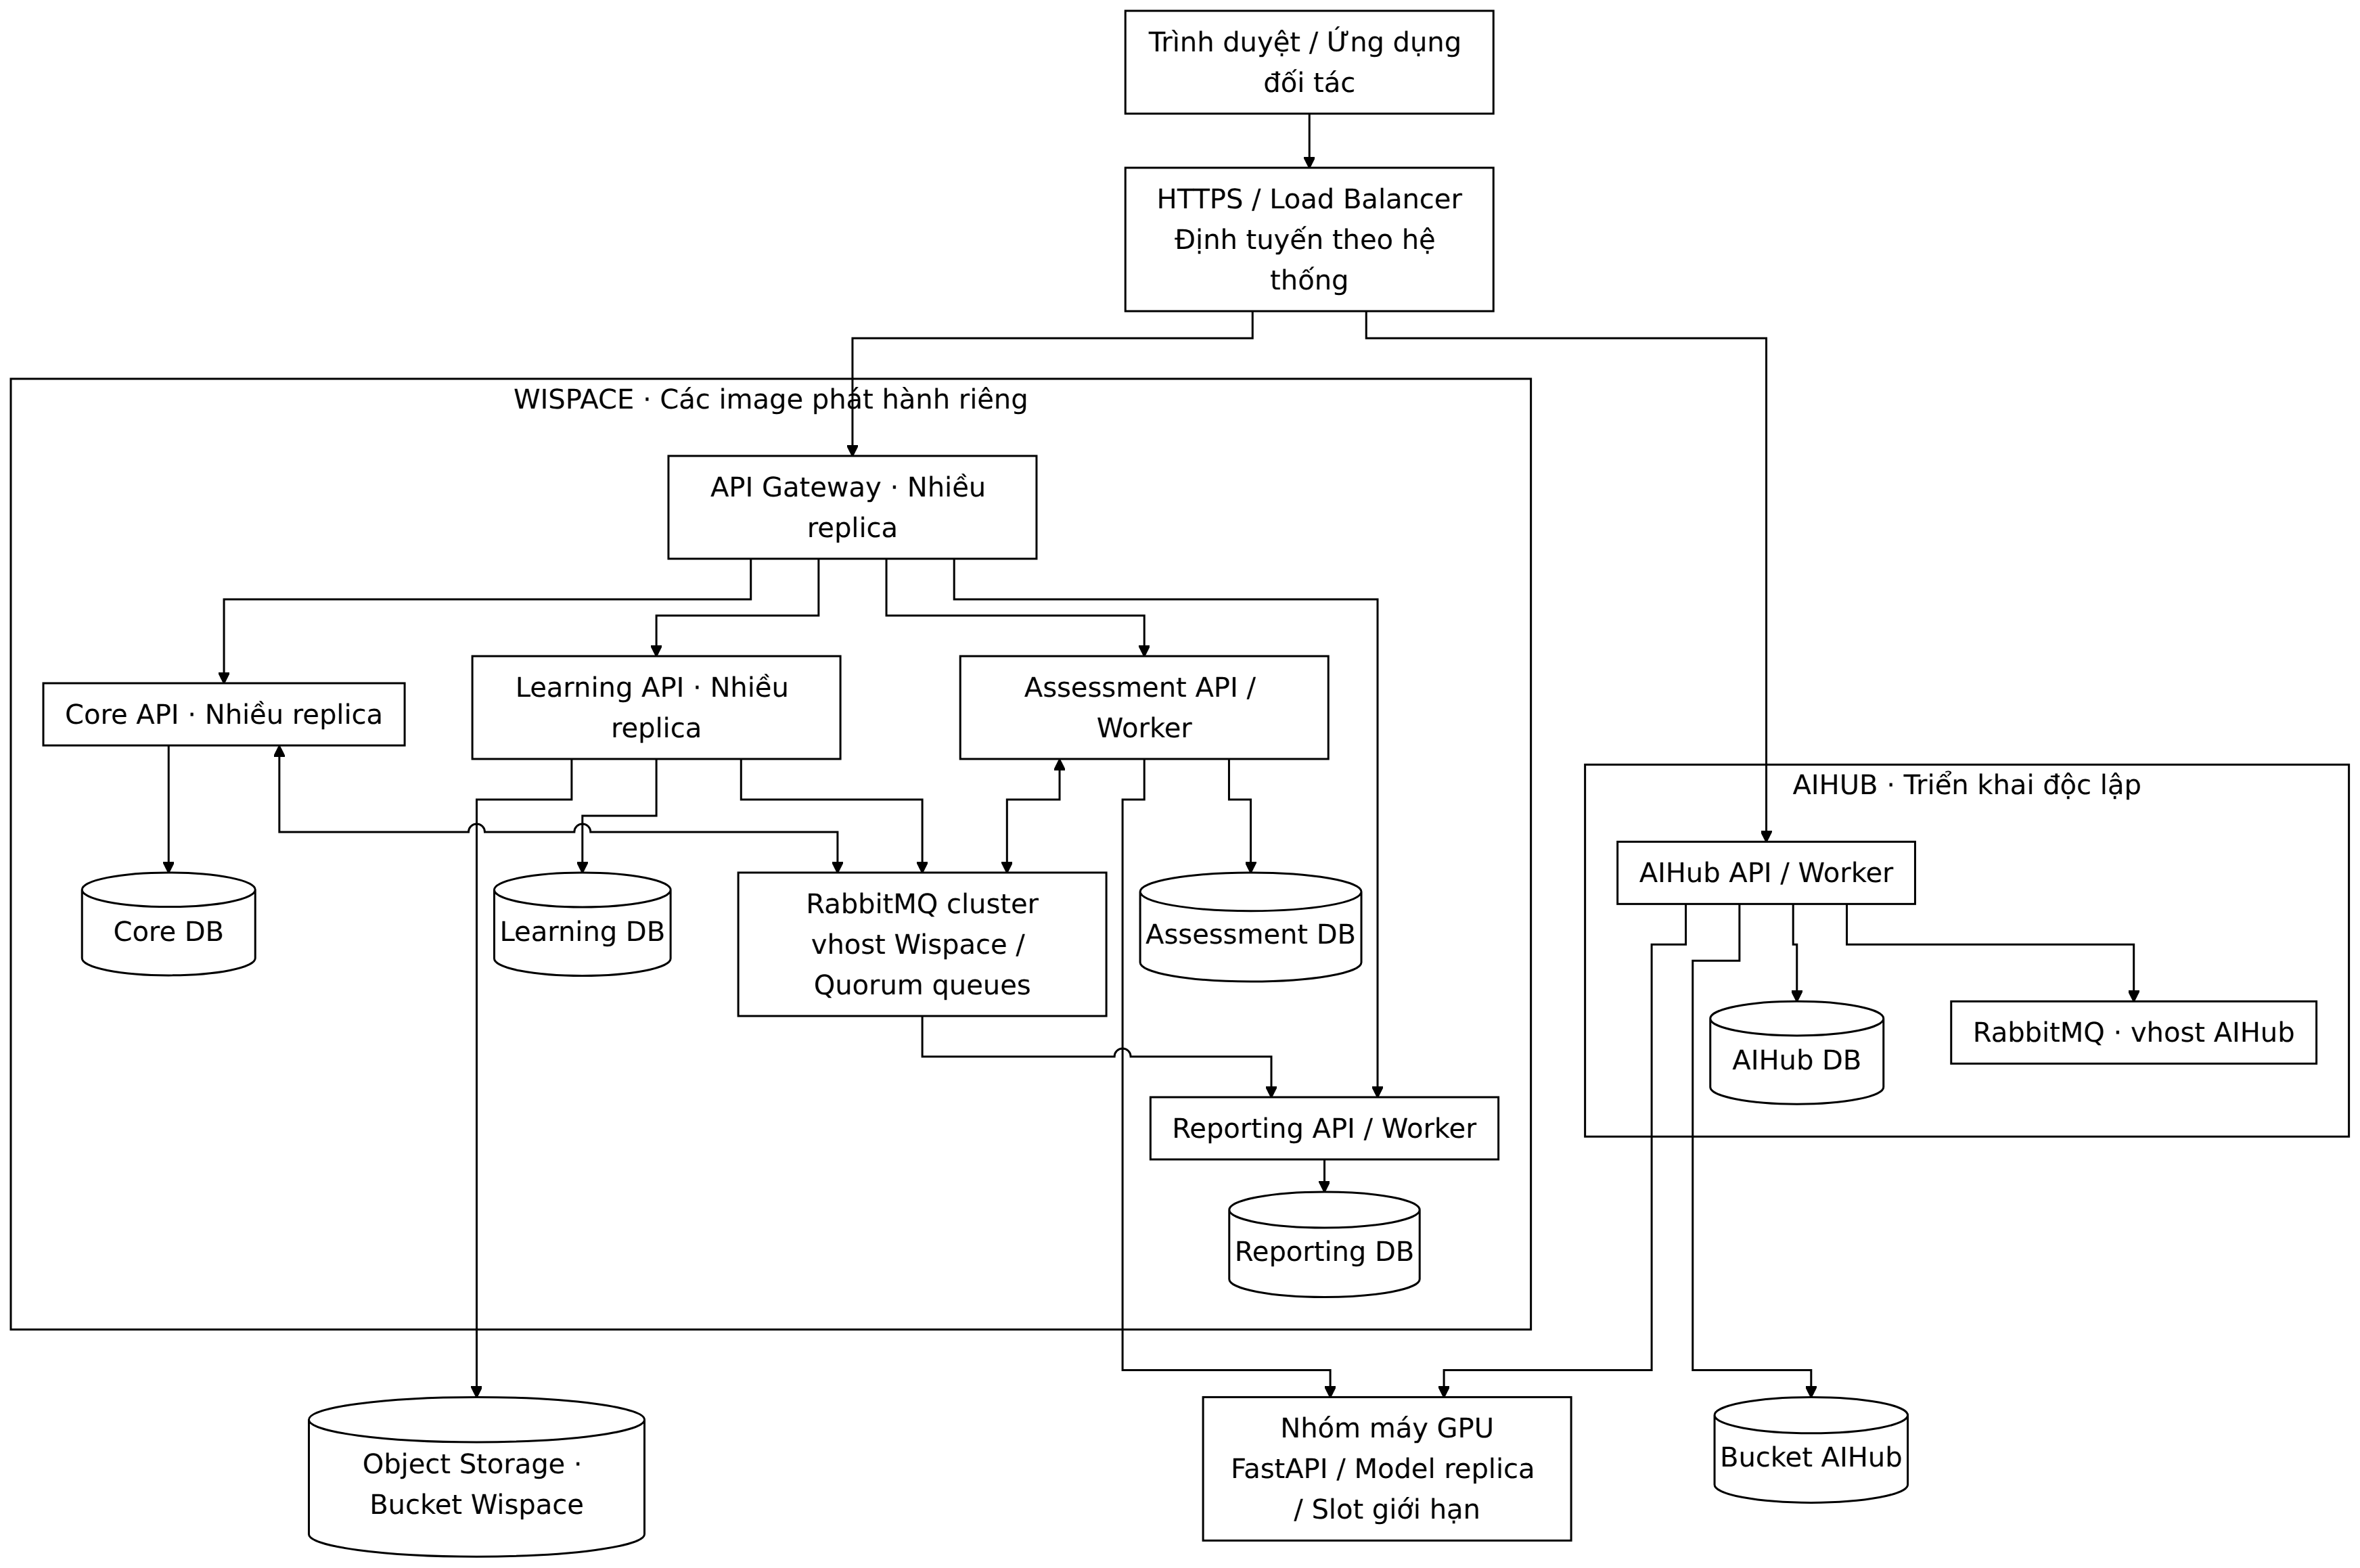
\includegraphics[width=\linewidth,height=.72\textheight,keepaspectratio]{Images/Design/deployment.png}
\caption{Mô hình triển khai ứng dụng và AI Runtime}
\label{design:fig:deployment}
\end{figure}

Việc đặt PostgreSQL và RabbitMQ cùng máy ứng dụng là lựa chọn cho môi trường thử nghiệm có quy mô nhỏ. Nếu máy này gặp sự cố, các thành phần cùng bị ảnh hưởng; bản triển khai đó chưa đủ để khẳng định đã đạt mục tiêu sẵn sàng hoặc chịu tải của Chương 5. Khi mở rộng, cơ sở dữ liệu, broker và ứng dụng có thể được triển khai trên các máy riêng hoặc dịch vụ được quản lý.

\paragraph*{Phân tách tải Wispace và B2B}

Các hàng đợi \texttt{speaking.\allowbreak{}assessment}, \texttt{b2b.\allowbreak{}inference} và \texttt{lab.\allowbreak{}generation} có cấu hình riêng về số Worker, prefetch và thời gian chờ. Các tác vụ Academic Lab hoặc đối tác không được sử dụng hết các slot suy luận dành cho lớp học và phiên thi đang hoạt động.

Khi dùng chung GPU, cần có cơ chế điều phối slot toàn cục ở lớp suy luận hoặc bộ lập lịch chung. Chỉ tách tên hàng đợi trong RabbitMQ chưa bảo đảm cô lập GPU. Trong bản triển khai đầu, có thể dành số slot cố định theo nhóm nguồn yêu cầu; số lượng cụ thể được xác định bằng thử nghiệm bộ nhớ và thời gian suy luận của mô hình.

Hệ thống giới hạn lượng công việc đang xử lý, theo dõi tuổi của công việc trong hàng đợi và áp dụng backpressure khi vượt ngưỡng. Mục tiêu mới là 1.000--10.000 người luyện/thi đồng thời; mức 200 phiên ở Chương 5 là kịch bản cơ sở cần nâng khi thống nhất yêu cầu. Kiểm thử lần lượt tải cơ sở, 1.000, 5.000 và 10.000 người theo tỷ lệ ghi âm/nộp bài thực tế, gồm đợt nộp đồng loạt và phục hồi kết nối. Đo p95/p99 API, lỗi, băng thông, connection pool, lock wait, tuổi công việc và thời gian chấm toàn luồng. Các mục tiêu 15 giây/câu, 3 phút/bài và 2 giây/chuyển câu vẫn là yêu cầu cần kiểm chứng; chưa có benchmark thì chưa thể cam kết số GPU, replica hoặc mức tải đạt được.

\paragraph*{Mở rộng API, dữ liệu và kết nối}

Core, Learning, Assessment API và Reporting API chạy stateless sau Gateway; trạng thái nghiệp vụ nằm trong database tương ứng. Redis có thể cache đề theo phiên bản, giới hạn tốc độ và dữ liệu đọc ngắn hạn; cache không quyết định bút toán quota. Truy vấn kết quả mới nhất đọc Assessment, còn biểu đồ xu hướng đọc Reporting và hiển thị thời điểm cập nhật khi projection chưa bắt kịp.

SignalR cần backplane hoặc dịch vụ quản lý kết nối khi chạy nhiều máy; cấu hình session affinity theo transport được sử dụng. Thông báo chỉ là tín hiệu để client đọc lại API nguồn; mất thông báo không làm mất kết quả. Tổng connection pool được giới hạn theo số replica và năng lực PostgreSQL, tránh tăng API gây cạn kết nối database. Hệ thống chia sẻ cấu hình xác thực/Data Protection phù hợp giữa các replica của cùng dịch vụ, dùng khóa dịch vụ và audience riêng khi giao tiếp nội bộ.

Autoscaling API dựa trên độ trễ, lưu lượng và tài nguyên; Worker dựa trên tuổi hàng đợi và năng lực GPU. Tăng Worker không được vượt tổng slot suy luận an toàn. Scale GPU cần tính thời gian nạp mô hình, bộ nhớ, độ dài audio và tỷ lệ retry. Admission control hạn chế mở phiên mới hoặc nhận chấm khi dự báo không đáp ứng được; không nhận vô hạn rồi xem việc lưu vào queue là đã đạt mục tiêu thời gian phản hồi.

\paragraph*{Cấu hình, backup và phát hành}

Connection string, bí mật OAuth, khóa PayOS và thông tin nhà cung cấp AI được cấu hình qua môi trường hoặc kho bí mật, tách khỏi Git. Mỗi môi trường có database, bucket, credentials và hạn mức riêng. FastAPI và các Worker có liveness/readiness probe phù hợp trạng thái kết nối và mô hình đã nạp.

PostgreSQL được backup định kỳ; bucket có chính sách bảo vệ và lưu trữ tương ứng. Quy trình khôi phục cần kiểm tra tính khớp giữa metadata trong database và object thực tế. Chỉ tạo được file backup chưa đủ để xác nhận có thể phục hồi toàn hệ thống.

Mỗi lần phát hành backend có bước kiểm tra migration trước khi đưa traffic vào. Mỗi phiên bản Scoring Model có artifact, checksum, cấu hình tiền xử lý và hợp đồng đầu ra tương ứng. Công việc đang chờ nên được gắn với phiên bản mô hình xác định, tránh thay đổi kết quả một cách khó truy vết khi chuyển phiên bản.

\subsubsection{Giám sát và xử lý sự cố}

\paragraph*{Dữ liệu quan sát hệ thống}

Mỗi yêu cầu có \texttt{trace\allowbreak{}Id} được truyền qua .NET, thông điệp RabbitMQ, Worker và FastAPI. Log có cấu trúc chứa định danh nghiệp vụ cần thiết nhưng không chứa bí mật xác thực, audio, URL ký trước hoặc toàn bộ nội dung nhạy cảm của người học.

Các nhóm chỉ số cần theo dõi gồm:

\begingroup\small\setstretch{1.1}
\begin{longtable}{|>{\raggedright\arraybackslash}p{\dimexpr 0.29\linewidth-2\tabcolsep-2\arrayrulewidth\relax}|>{\raggedright\arraybackslash}p{\dimexpr 0.71\linewidth-2\tabcolsep-2\arrayrulewidth\relax}|}
\caption{Dữ liệu quan sát hệ thống}\label{design:tab:6}\\
\hline
\textbf{Nhóm} & \textbf{Chỉ số chính} \\ \hline
\endfirsthead
\hline
\textbf{Nhóm} & \textbf{Chỉ số chính} \\ \hline
\endhead
\endfoot
API & Lưu lượng, thời gian đáp ứng, lỗi theo route, nguồn gọi và tổ chức. \\ \hline
Hàng đợi & Số công việc chờ, tuổi công việc, số đang chạy, số lần thử và công việc quá hạn. \\ \hline
Speaking & Thời gian chờ, tiền xử lý, suy luận, tỷ lệ lỗi audio và tỷ lệ job hoàn tất. \\ \hline
Mô hình/GPU & Phiên bản, bộ nhớ GPU, mức sử dụng, lỗi nạp mô hình và số slot khả dụng. \\ \hline
Nghiệp vụ & Lượt chấm, tỷ lệ hoàn quota, trạng thái thanh toán, mức sử dụng gói và chi phí ước tính. \\ \hline
Chất lượng & Sai lệch với nhãn chuyên gia, phân bố band, tỷ lệ thiếu tiêu chí và chất lượng theo nhóm dữ liệu. \\ \hline
\end{longtable}
\endgroup

Có thể bổ sung OpenTelemetry cho trace và metrics, cùng hệ thống hiển thị như Prometheus/Grafana khi cần. Bản đầu vẫn phải có log, định danh truy vết và các truy vấn vận hành cơ bản trước khi triển khai bộ dashboard đầy đủ.

\paragraph*{Chính sách xử lý sự cố}

\begingroup\small\setstretch{1.1}
\begin{longtable}{|>{\raggedright\arraybackslash}p{\dimexpr 0.29\linewidth-2\tabcolsep-2\arrayrulewidth\relax}|>{\raggedright\arraybackslash}p{\dimexpr 0.71\linewidth-2\tabcolsep-2\arrayrulewidth\relax}|}
\caption{Chính sách xử lý sự cố}\label{design:tab:7}\\
\hline
\textbf{Tình huống} & \textbf{Cách xử lý đề xuất} \\ \hline
\endfirsthead
\hline
\textbf{Tình huống} & \textbf{Cách xử lý đề xuất} \\ \hline
\endhead
\endfoot
RabbitMQ tạm thời không truy cập được & Giao dịch nhận bài và outbox đã ghi vẫn được giữ; Dispatcher thử phát lại. Theo dõi thời gian chưa phát để cảnh báo. \\ \hline
Worker dừng khi đang chấm & Lease hết hạn được phát hiện; công việc được khôi phục theo chính sách. Kết quả và quota có kiểm tra chống lặp. \\ \hline
Scoring Model quá tải & Giảm mức nhận việc, giữ job trong hàng đợi, ưu tiên slot Wispace và cập nhật trạng thái chờ. \\ \hline
Audio thiếu hoặc sai định dạng & Không chấm dữ liệu chưa đạt điều kiện; thông báo nguyên nhân, cho tải bù hoặc gửi lại khi phù hợp. \\ \hline
Phản hồi AI sai schema & Ghi lỗi hợp đồng, không lưu như kết quả hợp lệ; thử lại có giới hạn hoặc thất bại theo loại lỗi. \\ \hline
TTS lỗi & Dùng audio đã tạo trước hoặc nhà cung cấp TTS dự phòng đã cấu hình. \\ \hline
Object Storage lỗi & Giữ metadata ở trạng thái có thể khôi phục; không đánh dấu upload/xóa hoàn tất khi chưa xác nhận. \\ \hline
Redis lỗi & Dùng đường đọc PostgreSQL cho các chức năng được phép; chính sách giới hạn truy cập phải có hành vi dự phòng xác định. \\ \hline
PostgreSQL mất kết nối & Dừng nhận các thao tác cần đảm bảo nhất quán; không xác nhận đã giữ quota hoặc đã lưu kết quả khi chưa commit. \\ \hline
Callback thanh toán lặp & Xác minh và đối chiếu mã sự kiện; xử lý theo idempotency. \\ \hline
\end{longtable}
\endgroup

\paragraph*{Đánh giá và chuyển phiên bản mô hình}

Scoring Model mới được đánh giá trên bộ kiểm tra chuẩn không sử dụng để huấn luyện. Kết quả so sánh cần thể hiện sai lệch band, chất lượng theo tiêu chí, thời gian suy luận và khả năng xử lý dữ liệu của người học Việt Nam theo yêu cầu ở Chương 5.

Có thể chạy shadow trên một phần yêu cầu đủ điều kiện để so sánh phiên bản. Kết quả shadow không tiêu thụ thêm quota của người học và không tự ghi đè báo cáo chính. Khi phiên bản mới không đạt yêu cầu, model route được chuyển về phiên bản ổn định; mỗi kết quả đã lưu vẫn giữ phiên bản mô hình thực tế đã dùng.

\subsubsection{Kế hoạch hiện thực và thống nhất đặc tả}

\paragraph*{Thứ tự hiện thực đề xuất}

\begingroup\small\setstretch{1.1}
\begin{longtable}{|>{\raggedright\arraybackslash}p{\dimexpr 0.29\linewidth-2\tabcolsep-2\arrayrulewidth\relax}|>{\raggedright\arraybackslash}p{\dimexpr 0.71\linewidth-2\tabcolsep-2\arrayrulewidth\relax}|}
\caption{Thứ tự hiện thực đề xuất}\label{design:tab:8}\\
\hline
\textbf{Giai đoạn} & \textbf{Kết quả cần có} \\ \hline
\endfirsthead
\hline
\textbf{Giai đoạn} & \textbf{Kết quả cần có} \\ \hline
\endhead
\endfoot
1. Nền tảng và Wispace cơ bản & React Wispace, Core/Learning/Assessment/Reporting có dữ liệu riêng, Gateway, đăng nhập/phân quyền, kho đề, phiên thi và upload trực tiếp; AIHub có frontend và backend riêng. \\ \hline
2. Chấm Speaking và báo cáo & RabbitMQ, outbox, Worker, tích hợp Scoring Model, idempotency, quota, tiến trình và kết quả. \\ \hline
3. AIHub B2B & Tổ chức, credentials, danh mục API/mô hình, quyền dịch vụ, hạn mức, API đồng bộ/bất đồng bộ và usage. \\ \hline
4. Công cụ nội bộ và vận hành & Academic Lab, xuất dữ liệu có kiểm soát, giám sát, backup/restore, đánh giá mô hình và hoàn thiện phân tách tải. \\ \hline
\end{longtable}
\endgroup

Các giai đoạn là thứ tự đề xuất để triển khai đồ án, không phải trạng thái hiện thực đã được xác nhận. Các mục tiêu như độ lệch band, thời gian chấm và mức tải được kiểm thử sau khi có mô hình và môi trường chạy thực tế.

\paragraph*{Các điểm cần thống nhất khi đưa vào báo cáo chính}

\begingroup\small\setstretch{1.1}
\begin{longtable}{|>{\raggedright\arraybackslash}p{\dimexpr 0.29\linewidth-2\tabcolsep-2\arrayrulewidth\relax}|>{\raggedright\arraybackslash}p{\dimexpr 0.71\linewidth-2\tabcolsep-2\arrayrulewidth\relax}|}
\caption{Các điểm cần thống nhất khi đưa vào báo cáo chính}\label{design:tab:9}\\
\hline
\textbf{Nội dung} & \textbf{Cách thống nhất trong thiết kế này} \\ \hline
\endfirsthead
\hline
\textbf{Nội dung} & \textbf{Cách thống nhất trong thiết kế này} \\ \hline
\endhead
\endfoot
Vai trò của AIHub & Xác định AIHub là cổng quản lý/cung cấp API mô hình B2B; Academic Lab thuộc công cụ nội bộ. \\ \hline
Backend hai hệ thống & Wispace dùng microservices theo nhóm nghiệp vụ; AIHub dùng modular monolith riêng. Hai frontend, danh tính, hạn mức và triển khai độc lập. \\ \hline
Đường gọi AI Wispace & Assessment Worker của Wispace gọi trực tiếp FastAPI, không qua đường API B2B. \\ \hline
Xác thực Portal & Mỗi hệ thống xác thực riêng; thống nhất mô tả token và cookie trong đặc tả của từng hệ thống, không dùng chung phiên đăng nhập. \\ \hline
Số lần thử chấm & Trong thiết kế đề xuất: tối đa ba lần thực thi tự động, gồm một lần đầu và hai lần thử lại; sửa các chỗ dùng từ “retry” chưa cùng nghĩa khi đồng bộ Chương 5–6. \\ \hline
Hạn mức Speaking và B2B & Hai sổ hạn mức riêng theo người học và tổ chức; chi phí mô hình có thể được thống kê theo cùng nguồn tính toán. \\ \hline
Lưu trữ và quyền riêng tư & Audio riêng tư, link đọc tối đa 10 phút, xóa theo chính sách 180 ngày, đồng ý huấn luyện tách riêng đồng ý xử lý. \\ \hline
Mô hình chấm Speaking & Giữ giả định mô hình tự huấn luyện; chương thiết kế mô tả tích hợp và vận hành, không khẳng định chất lượng đã được thực nghiệm. \\ \hline
\end{longtable}
\endgroup

Chương này sử dụng thiết kế đề xuất Wispace–AIHub làm cơ sở hiện thực. Những điểm khác biệt so với các đặc tả ở Chương 5–6 được ghi rõ trong bảng trên để thống nhất khi triển khai; các mục tiêu hiệu năng và chất lượng cần được kiểm chứng bằng thực nghiệm.

\clearpage
\subsection{Kết chương}

Thiết kế đề xuất tổ chức Wispace và AIHub thành hai hệ thống độc lập, Wispace có frontend React và các microservice .NET với PostgreSQL sở hữu riêng; AIHub có frontend và backend modular monolith độc lập. Python FastAPI triển khai các năng lực AI theo hợp đồng dịch vụ. Wispace giữ vai trò sản phẩm học tập chính và gọi trực tiếp dịch vụ chấm Speaking; AIHub cung cấp cơ chế khai thác mô hình cho tổ chức B2B và các công cụ quản trị nội bộ.

Việc tách tác vụ chấm qua Worker và hàng đợi, quản lý audio bằng Object Storage, ghi nhận quota theo giao dịch và theo dõi phiên bản mô hình tạo cơ sở để hiện thực hệ thống có thể khôi phục và truy vết. Các thành phần triển khai, hợp đồng dữ liệu và chính sách vận hành trong chương là căn cứ cho quá trình xây dựng và đánh giá hệ thống ở các chương tiếp theo.



% Sections/08-CaiDatHeThong.tex
% Chương 8 – Cài đặt hệ thống
%=========================

\section{Cài đặt hệ thống}

Chương này trình bày cách hệ thống được đóng gói và triển khai bằng Docker trên Google Cloud Platform. Nội dung tập trung vào môi trường triển khai, cấu hình tài nguyên, cách chạy các container và thứ tự khởi động các thành phần chính.
\subsection{Chuẩn bị dữ liệu đầu vào cho database}

Dữ liệu sản phẩm ban đầu của hệ thống được lấy từ bộ dữ liệu Fashion Product Images Dataset trên Kaggle. Bộ dữ liệu này cung cấp khoảng 44 nghìn sản phẩm thời trang, bao gồm ảnh sản phẩm, nhãn danh mục, mô tả và một số thuộc tính liên quan \parencite{paramaggarwalFashionProductImages}.

Trong phạm vi đồ án, hệ thống không sử dụng toàn bộ dữ liệu gốc mà chỉ chọn 900 sản phẩm làm dữ liệu đầu vào để xây dựng database thử nghiệm. Các sản phẩm này được chuẩn hóa và import vào MySQL nhằm phục vụ các chức năng chính như hiển thị sản phẩm, quản lý danh mục, tìm kiếm, lọc sản phẩm và đồng bộ dữ liệu sang AI Service.

Sau khi dữ liệu được import vào MySQL, database được export thành file \texttt{backup.sql}. File này tiếp tục được sử dụng làm đầu vào cho pipeline Việt hóa dữ liệu bằng Qwen3.5-9B ở bước xử lý tiếp theo.

\begin{table}[H]
\centering
\caption{Nguồn dữ liệu đầu vào cho database thử nghiệm}
\label{tab:database-input-dataset}
\begin{tabularx}{\linewidth}{@{}p{0.30\linewidth}X@{}}
\toprule
\textbf{Thành phần} & \textbf{Mô tả} \\
\midrule
Nguồn dữ liệu & Fashion Product Images Dataset trên Kaggle \\
Quy mô dữ liệu gốc & Khoảng 44 nghìn sản phẩm thời trang \\
Dữ liệu sử dụng trong đồ án & 900 sản phẩm được chọn để xây dựng database thử nghiệm \\
Vai trò & Là dữ liệu đầu vào cho MySQL, phục vụ kiểm thử các chức năng sản phẩm, tìm kiếm và AI Service \\
Đầu ra sau xử lý & File \texttt{backup.sql} dùng cho pipeline Việt hóa dữ liệu \\
\bottomrule
\end{tabularx}
\end{table}
\subsection{Cài đặt pipeline Việt hóa dữ liệu bằng Qwen3.5}

Để hỗ trợ giao diện tiếng Việt, tìm kiếm tiếng Việt và dữ liệu đầu vào cho AI Service, hệ thống sử dụng pipeline Việt hóa dữ liệu sản phẩm bằng mô hình Qwen3.5-9B. Pipeline được chạy trên Kaggle Notebook với GPU Tesla T4, dữ liệu đầu vào là file backup MySQL \texttt{backup.sql}, dữ liệu đầu ra là file \texttt{vi\_updates.sql} dùng để cập nhật các trường tiếng Việt vào MySQL.

Pipeline gồm ba bước chính: trích xuất dữ liệu cần dịch từ file SQL, sử dụng Qwen3.5-9B để dịch sản phẩm và danh mục, sau đó sinh file SQL cập nhật dữ liệu tiếng Việt.

\begin{lstlisting}[language=Python,caption={Cấu hình đường dẫn và mô hình cho pipeline Việt hóa dữ liệu},label={lst:vi-pipeline-config}]
PIPE = "/kaggle/input/datasets/anhdngltrn/okneokok/dacn_vi_llm_pipeline_qwen3/dacn_vi_llm_pipeline_qwen3"
SQL = "/kaggle/input/datasets/anhdngltrn/okneokok/backup.sql"
MODEL = "Qwen/Qwen3.5-9B"
BATCH = 2
\end{lstlisting}

Trước khi chạy pipeline, môi trường được cài đặt các thư viện cần thiết để nạp mô hình, lượng tử hóa 4-bit và suy luận trên GPU.

\begin{lstlisting}[style=terminal,caption={Cài đặt thư viện phục vụ suy luận Qwen3.5-9B},label={lst:vi-install-deps}]
pip install -q -U git+https://github.com/huggingface/transformers.git accelerate bitsandbytes sentencepiece protobuf
\end{lstlisting}

Đầu tiên, pipeline trích xuất dữ liệu cần dịch từ file \texttt{backup.sql}. Kết quả bước này tạo ra 900 job sản phẩm và 79 job danh mục.

\begin{lstlisting}[style=terminal,caption={Trích xuất job dịch từ file backup SQL},label={lst:vi-extract-jobs}]
rm -rf /kaggle/working/translation_jobs

python "$PIPE/00_extract_jobs.py" \
  --sql "$SQL" \
  --out-dir /kaggle/working/translation_jobs

wc -l /kaggle/working/translation_jobs/product_jobs.jsonl
wc -l /kaggle/working/translation_jobs/category_jobs.jsonl
\end{lstlisting}

Để tận dụng hai GPU Tesla T4, danh sách job sản phẩm được chia thành hai phần, mỗi phần gồm 450 job.

\begin{lstlisting}[style=terminal,caption={Chia job sản phẩm thành hai shard để xử lý song song},label={lst:vi-split-shards}]
mkdir -p /kaggle/working/shards_qwen35_full

awk 'NR % 2 == 1' /kaggle/working/translation_jobs/product_jobs.jsonl \
  > /kaggle/working/shards_qwen35_full/product_gpu0.jsonl

awk 'NR % 2 == 0' /kaggle/working/translation_jobs/product_jobs.jsonl \
  > /kaggle/working/shards_qwen35_full/product_gpu1.jsonl

wc -l /kaggle/working/shards_qwen35_full/product_gpu0.jsonl
wc -l /kaggle/working/shards_qwen35_full/product_gpu1.jsonl
\end{lstlisting}

Sau đó, hai tiến trình dịch sản phẩm được chạy song song trên hai GPU. Mô hình được nạp với lượng tử hóa 4-bit để giảm mức sử dụng bộ nhớ GPU.

\begin{lstlisting}[style=terminal,caption={Dịch dữ liệu sản phẩm song song bằng Qwen3.5-9B trên hai GPU},label={lst:vi-translate-products}]
PIPE="/kaggle/input/datasets/anhdngltrn/okneokok/dacn_vi_llm_pipeline_qwen3/dacn_vi_llm_pipeline_qwen3"
MODEL="Qwen/Qwen3.5-9B"
BATCH=2

CUDA_VISIBLE_DEVICES=0 python "$PIPE/01_translate_llm_kaggle.py" \
  --jobs /kaggle/working/shards_qwen35_full/product_gpu0.jsonl \
  --output /kaggle/working/product_translations_gpu0_qwen35_full.jsonl \
  --model "$MODEL" \
  --batch-size "$BATCH" \
  --quantization 4bit \
  --max-new-tokens 2048 \
  --trust-remote-code \
  > /kaggle/working/gpu0_qwen35_full.log 2>&1 &

CUDA_VISIBLE_DEVICES=1 python "$PIPE/01_translate_llm_kaggle.py" \
  --jobs /kaggle/working/shards_qwen35_full/product_gpu1.jsonl \
  --output /kaggle/working/product_translations_gpu1_qwen35_full.jsonl \
  --model "$MODEL" \
  --batch-size "$BATCH" \
  --quantization 4bit \
  --max-new-tokens 2048 \
  --trust-remote-code \
  > /kaggle/working/gpu1_qwen35_full.log 2>&1 &

wait

echo "PRODUCT RUN DONE"
\end{lstlisting}

Kết quả từ hai GPU được gộp lại và loại bỏ các bản ghi trùng lặp theo \texttt{job\_id}.

\begin{lstlisting}[language=Python,caption={Gộp và loại bỏ trùng lặp kết quả dịch sản phẩm},label={lst:vi-merge-products}]
import json
from pathlib import Path

inp = Path("/kaggle/working/product_translations_raw.jsonl")
out = Path("/kaggle/working/product_translations.jsonl")

seen = set()
rows = []

with inp.open("r", encoding="utf-8") as f:
    for line in f:
        if not line.strip():
            continue
        try:
            obj = json.loads(line)
            jid = obj.get("job_id")
            if not jid or jid in seen:
                continue
            seen.add(jid)
            rows.append(obj)
        except Exception:
            pass

with out.open("w", encoding="utf-8") as f:
    for obj in rows:
        f.write(json.dumps(obj, ensure_ascii=False) + "\n")

print("unique product translations:", len(rows))
\end{lstlisting}

Sau lần chạy đầu, pipeline dịch được 882 trên tổng số 900 sản phẩm. Các job còn thiếu được tách riêng để chạy lại.

\begin{lstlisting}[language=Python,caption={Kiểm tra các job sản phẩm chưa được dịch thành công},label={lst:vi-check-missing}]
import json
from pathlib import Path

jobs_path = Path("/kaggle/working/translation_jobs/product_jobs.jsonl")
done_path = Path("/kaggle/working/product_translations.jsonl")
missing_path = Path("/kaggle/working/product_jobs_missing.jsonl")

done = set()

with done_path.open("r", encoding="utf-8") as f:
    for line in f:
        if line.strip():
            try:
                done.add(json.loads(line)["job_id"])
            except Exception:
                pass

total = 0
missing = 0

with jobs_path.open("r", encoding="utf-8") as fin, missing_path.open("w", encoding="utf-8") as fout:
    for line in fin:
        if not line.strip():
            continue
        total += 1
        obj = json.loads(line)
        if obj["job_id"] not in done:
            fout.write(json.dumps(obj, ensure_ascii=False) + "\n")
            missing += 1

print("total:", total)
print("done:", len(done))
print("missing:", missing)
print("missing file:", missing_path)
\end{lstlisting}

Các job lỗi được chạy lại với \texttt{batch-size=1} và số lần retry lớn hơn để giảm lỗi mô hình trả về sai định dạng JSON.

\begin{lstlisting}[style=terminal,caption={Chạy lại các job sản phẩm bị lỗi với batch-size nhỏ hơn},label={lst:vi-retry-missing}]
CUDA_VISIBLE_DEVICES=0 python "$PIPE/01_translate_llm_kaggle.py" \
  --jobs /kaggle/working/product_jobs_missing.jsonl \
  --output /kaggle/working/product_translations_missing_retry.jsonl \
  --model "$MODEL" \
  --batch-size 1 \
  --quantization 4bit \
  --max-new-tokens 2048 \
  --trust-remote-code \
  --retries 5
\end{lstlisting}

Sau bước retry, số bản dịch sản phẩm duy nhất đạt 891. Đối với danh mục, pipeline dịch trực tiếp toàn bộ 79 job danh mục.

\begin{lstlisting}[style=terminal,caption={Dịch dữ liệu danh mục sản phẩm bằng Qwen3.5-9B},label={lst:vi-translate-categories}]
CUDA_VISIBLE_DEVICES=0 python "$PIPE/01_translate_llm_kaggle.py" \
  --jobs /kaggle/working/translation_jobs/category_jobs.jsonl \
  --output /kaggle/working/category_translations.jsonl \
  --model "$MODEL" \
  --batch-size 2 \
  --quantization 4bit \
  --max-new-tokens 1024 \
  --trust-remote-code

wc -l /kaggle/working/category_translations.jsonl
\end{lstlisting}

Cuối cùng, script \texttt{02\_make\_update\_sql.py} được dùng để sinh file SQL cập nhật dữ liệu tiếng Việt vào MySQL.

\begin{lstlisting}[style=terminal,caption={Sinh file SQL cập nhật dữ liệu tiếng Việt vào MySQL},label={lst:vi-make-update-sql}]
python "$PIPE/02_make_update_sql.py" \
  --translations /kaggle/working/category_translations.jsonl /kaggle/working/product_translations_final.jsonl \
  --output /kaggle/working/vi_updates.sql

ls -lh /kaggle/working/vi_updates.sql
head -n 40 /kaggle/working/vi_updates.sql
\end{lstlisting}

File \texttt{vi\_updates.sql} bổ sung các cột tiếng Việt nếu chưa tồn tại, sau đó cập nhật dữ liệu đã dịch vào các bảng tương ứng.

\begin{lstlisting}[language=SQL,caption={Một phần file SQL cập nhật dữ liệu tiếng Việt},label={lst:vi-update-sql-head}]
-- Generated by 02_make_update_sql.py
SET NAMES utf8mb4;
SET FOREIGN_KEY_CHECKS=0;

-- Add Vietnamese columns if missing
SET @col_exists := (
  SELECT COUNT(*) FROM INFORMATION_SCHEMA.COLUMNS
  WHERE TABLE_SCHEMA = DATABASE()
    AND TABLE_NAME = 'products'
    AND COLUMN_NAME = 'product_display_name_vi'
);

SET @ddl := IF(
  @col_exists = 0,
  'ALTER TABLE `products` ADD COLUMN `product_display_name_vi` varchar(255) CHARACTER SET utf8mb4 COLLATE utf8mb4_unicode_ci NULL',
  'SELECT 1'
);

PREPARE stmt FROM @ddl;
EXECUTE stmt;
DEALLOCATE PREPARE stmt;
\end{lstlisting}

Kết quả thực thi pipeline được tổng hợp trong \Cref{tab:vi-pipeline-result}.

\begin{table}[H]
\centering
\caption{Kết quả thực thi pipeline Việt hóa dữ liệu bằng Qwen3.5-9B}
\label{tab:vi-pipeline-result}
\begin{tabularx}{\linewidth}{@{}p{0.45\linewidth}p{0.18\linewidth}X@{}}
\toprule
\textbf{Hạng mục} & \textbf{Kết quả} & \textbf{Ghi chú} \\
\midrule
Job sản phẩm được trích xuất & 900 & Sinh từ file backup SQL. \\
Job danh mục được trích xuất & 79 & Sinh từ dữ liệu danh mục. \\
Bản dịch sản phẩm sau lần chạy đầu & 882 & Sau khi gộp kết quả từ hai GPU. \\
Job sản phẩm còn thiếu & 18 & Được tách riêng để retry. \\
Bản dịch sản phẩm cuối cùng & 891 & Sau khi retry với batch-size nhỏ hơn. \\
Bản dịch danh mục & 79 & Dịch thành công toàn bộ danh mục. \\
Dòng cập nhật sản phẩm & 871 & Sinh vào file \texttt{vi\_updates.sql}. \\
Dòng cập nhật danh mục & 79 & Sinh vào file \texttt{vi\_updates.sql}. \\
Dòng cập nhật thuộc tính & 2528 & Cập nhật các thuộc tính đã Việt hóa. \\
\bottomrule
\end{tabularx}
\end{table}


Sau khi sinh file SQL, các kết quả đầu ra được đóng gói để tải về và import vào MySQL.

\begin{lstlisting}[style=terminal,caption={Đóng gói kết quả đầu ra của pipeline Việt hóa dữ liệu},label={lst:vi-zip-output}]
cd /kaggle/working

zip -q dacn_vi_outputs.zip \
  vi_updates.sql \
  product_translations_final.jsonl \
  category_translations.jsonl \
  product_jobs_missing.jsonl \
  product_translations_missing_retry.jsonl \
  gpu0_qwen35_full.log \
  gpu1_qwen35_full.log

ls -lh /kaggle/working/dacn_vi_outputs.zip
\end{lstlisting}

File \texttt{vi\_updates.sql} được import vào MySQL để bổ sung tên sản phẩm, danh mục và thuộc tính tiếng Việt. Dữ liệu này được sử dụng cho frontend, tìm kiếm văn bản tiếng Việt và các chức năng AI liên quan đến hiểu truy vấn người dùng.
\subsection{Cài đặt fine-tune YOLOv26}
Để mô hình phù hợp hơn với miền dữ liệu thương mại điện tử thời trang, YOLOv26 được fine-tune trên tập dữ liệu thời trang được xây dựng dựa trên nguồn Fashionpedia. Fashionpedia là bộ dữ liệu thị giác máy tính trong lĩnh vực thời trang, cung cấp dữ liệu ảnh cùng annotation phục vụ các bài toán như phát hiện đối tượng, phân đoạn đối tượng và nhận diện thuộc tính thời trang \parencite{jia2020fashionpedia}. Trong quá trình huấn luyện, dữ liệu được chuyển đổi về định dạng YOLO và gom thành bốn nhóm nhãn chính: \textit{accessories}, \textit{bags}, \textit{clothing} và \textit{shoes}. Các nhóm nhãn này tương ứng với những loại sản phẩm phổ biến trong hệ thống, đồng thời đủ tổng quát để hỗ trợ chức năng tìm kiếm bằng hình ảnh.

Nguồn dữ liệu được tham khảo từ phiên bản Fashionpedia được công bố trên Hugging Face Datasets. Bộ dữ liệu này thuộc nhóm dữ liệu ảnh cho bài toán object detection, có định dạng lưu trữ Parquet và giấy phép CC-BY-4.0 \parencite{huggingfaceFashionpedia}.



Trước khi huấn luyện, môi trường cần cài đặt thư viện \texttt{ultralytics} để sử dụng API huấn luyện mô hình YOLO. Lệnh cài đặt được trình bày trong \Cref{lst:install-ultralytics}.

\begin{lstlisting}[style=terminal,caption={Cài đặt thư viện Ultralytics phục vụ fine-tune YOLOv26},label={lst:install-ultralytics}]
pip install -U ultralytics
\end{lstlisting}

Tập dữ liệu được tổ chức theo định dạng YOLO, gồm ba tập con là train, validation và test. File cấu hình dữ liệu được tạo bằng đoạn mã trong \Cref{lst:yolo-data-yaml}.

\begin{lstlisting}[language=Python,caption={Tạo file cấu hình dữ liệu cho fine-tune YOLOv26},label={lst:yolo-data-yaml}]
import os

yaml_text = """
train: /kaggle/input/datasets/anhdngltrn/dungne/fashion_dataset/train/images
val: /kaggle/input/datasets/anhdngltrn/dungne/fashion_dataset/val/images
test: /kaggle/input/datasets/anhdngltrn/dungne/fashion_dataset/test/images

nc: 4
names:
  0: accessories
  1: bags
  2: clothing
  3: shoes
""".strip()

with open("/kaggle/working/data.yaml", "w") as f:
    f.write(yaml_text)

print("Saved /kaggle/working/data.yaml")
print(open("/kaggle/working/data.yaml").read())
\end{lstlisting}

Sau khi chuẩn bị file cấu hình dữ liệu, mô hình YOLOv26s được nạp từ weight ban đầu \texttt{yolo26s.pt}. Quá trình huấn luyện kiểm tra GPU khả dụng, cấu hình thiết bị huấn luyện và thực hiện fine-tune trên tập dữ liệu đã chuẩn bị. Đoạn mã huấn luyện được trình bày trong \Cref{lst:yolo-train}.

\begin{lstlisting}[language=Python,caption={Fine-tune mô hình YOLOv26s trên tập dữ liệu thời trang},label={lst:yolo-train}]
import torch
from ultralytics import YOLO

DATA_YAML = "/kaggle/working/data.yaml"

print("CUDA available:", torch.cuda.is_available())
print("GPU count:", torch.cuda.device_count())

for i in range(torch.cuda.device_count()):
    print(f"GPU {i}: {torch.cuda.get_device_name(i)}")

ngpu = torch.cuda.device_count()
device_cfg = [0, 1] if ngpu >= 2 else 0
batch_size = 24
worker_size = 12

model = YOLO("yolo26s.pt")

results = model.train(
    data=DATA_YAML,
    epochs=40,
    imgsz=640,
    batch=batch_size,
    device=device_cfg,
    workers=worker_size,
    pretrained=True,
    patience=8,
    project="/kaggle/working",
    name="yolo26s_run2",
    val=True,
    amp=True,
    save=True,
    save_period=1,
    verbose=True
)
\end{lstlisting}

Trong cấu hình trên, mô hình được huấn luyện trong 40 epoch với kích thước ảnh đầu vào là \texttt{640}. Tham số \texttt{pretrained=True} cho phép mô hình kế thừa trọng số đã học trước đó, giúp quá trình fine-tune phù hợp hơn so với huấn luyện lại từ đầu. Tham số \texttt{patience=8} được dùng để dừng sớm khi kết quả đánh giá không cải thiện, còn \texttt{amp=True} giúp tăng tốc huấn luyện bằng mixed precision trên GPU.

Sau khi huấn luyện, kết quả đánh giá mô hình được trình bày trong \Cref{tab:yolov26-finetune-result}. Do bài toán phát hiện đối tượng không sử dụng độ chính xác theo nghĩa phân loại thông thường, hệ thống đánh giá mô hình thông qua các chỉ số Precision, Recall, mAP50 và mAP50-95.

\begin{table}[H]
\centering
\caption{Kết quả đánh giá mô hình YOLOv26 sau khi fine-tune trên tập dữ liệu thời trang}
\label{tab:yolov26-finetune-result}
\begin{tabularx}{\linewidth}{@{}p{0.18\linewidth}p{0.11\linewidth}p{0.14\linewidth}p{0.13\linewidth}p{0.12\linewidth}p{0.13\linewidth}X@{}}
\toprule
\textbf{Lớp} & \textbf{Ảnh} & \textbf{Đối tượng} & \textbf{Precision} & \textbf{Recall} & \textbf{mAP50} & \textbf{mAP50-95} \\
\midrule
Tất cả & 2339 & 8226 & 0.875 & 0.760 & 0.849 & 0.685 \\
Accessories & 932 & 1428 & 0.806 & 0.587 & 0.695 & 0.512 \\
Bags & 367 & 384 & 0.842 & 0.694 & 0.807 & 0.604 \\
Clothing & 2339 & 3966 & 0.926 & 0.882 & 0.947 & 0.861 \\
Shoes & 1267 & 2448 & 0.924 & 0.880 & 0.945 & 0.763 \\
\bottomrule
\end{tabularx}
\end{table}

Kết quả cho thấy mô hình đạt Precision tổng thể là 0.875, Recall là 0.760, mAP50 đạt 0.849 và mAP50-95 đạt 0.685. Trong đó, hai nhóm \textit{clothing} và \textit{shoes} có kết quả tốt nhất với mAP50 lần lượt là 0.947 và 0.945. Điều này cho thấy mô hình nhận diện tốt các sản phẩm có hình dạng rõ ràng và số lượng mẫu tương đối lớn trong tập dữ liệu.

Đối với nhóm \textit{accessories}, kết quả thấp hơn với mAP50-95 đạt 0.512. Nguyên nhân có thể đến từ việc phụ kiện thường có kích thước nhỏ, hình dạng đa dạng và dễ bị nhiễu bởi nền ảnh hoặc các vật thể khác. Tuy nhiên, với mục tiêu chính là phát hiện vùng sản phẩm để crop ảnh trước khi tạo image embedding, kết quả tổng thể vẫn đáp ứng được yêu cầu tiền xử lý ảnh cho chức năng tìm kiếm bằng hình ảnh.

Bên cạnh độ chính xác phát hiện đối tượng, mô hình cũng có thời gian suy luận thấp, với thời gian inference trung bình khoảng 1.8ms trên mỗi ảnh trong môi trường đánh giá. Điều này cho thấy mô hình phù hợp để tích hợp vào AI Service nhằm hỗ trợ xử lý ảnh trong luồng image search và hybrid search.

Sau khi huấn luyện, weight tốt nhất của mô hình được sử dụng trong AI Service. File weight có thể được lưu trong thư mục model của service như \Cref{lst:yolo-weight-path}.

\begin{lstlisting}[style=terminal,caption={Đường dẫn lưu weight YOLOv26 sau khi fine-tune},label={lst:yolo-weight-path}]
ai-service/models/yolov26/best.pt
\end{lstlisting}

Khi AI Service khởi động, mô hình YOLOv26 fine-tuned được load từ file weight này. Trong luồng tìm kiếm bằng hình ảnh, service nhận ảnh từ Spring Boot Backend, phát hiện vùng sản phẩm bằng YOLOv26, crop ảnh nếu phát hiện thành công, sau đó tạo image embedding và truy vấn Qdrant để tìm các sản phẩm tương đồng.

Trong trường hợp YOLOv26 không phát hiện được vùng sản phẩm hoặc điểm tin cậy thấp, AI Service sử dụng ảnh gốc làm fallback để tiếp tục tạo image embedding. 
\subsection{Môi trường triển khai}

Hệ thống được triển khai trên Google Cloud Platform tại khu vực \texttt{asia-southeast1} tương ứng Singapore.

Các thành phần được chạy dưới dạng Docker container gồm:

\begin{itemize}
    \item Backend Spring Boot.
    \item FastAPI AI Service.
    \item Frontend React.
    \item MySQL database.
    \item Qdrant vector database.
\end{itemize}

\subsection{Cấu hình tài nguyên}

Bảng \ref{tab:resource-config} trình bày cấu hình tài nguyên dự kiến cho môi trường demo của hệ thống. Do hệ thống phục vụ kiểm thử và báo cáo đồ án, tài nguyên được lựa chọn ở mức tiết kiệm, riêng FastAPI AI Service có sử dụng GPU để hỗ trợ xử lý embedding và mô hình AI.

\begin{table}[H]
\centering
\caption{Cấu hình tài nguyên triển khai hệ thống}
\label{tab:resource-config}
\begin{tabular}{|p{4cm}|p{3cm}|p{3cm}|p{4cm}|}
\hline
\textbf{Thành phần} & \textbf{CPU} & \textbf{RAM} & \textbf{Lưu trữ / GPU} \\ \hline
Spring Boot Backend & 1 vCPU & 1 GB & 10 GB SSD \\ \hline
FastAPI AI Service & 1--2 vCPU & 4 GB & 20 GB SSD, 1 GPU \\ \hline
MySQL & 1 vCPU & 1 GB & 20 GB SSD \\ \hline
Qdrant & 1 vCPU & 2 GB & 20 GB SSD \\ \hline
\end{tabular}
\end{table}


\subsection{Đóng gói và chạy Docker}


Các image chính gồm:

\begin{itemize}
    \item \texttt{service-api-ecommerce}: image backend Spring Boot.
    \item \texttt{service-ai}: image FastAPI AI Service.
    \item \texttt{mysql}: image cơ sở dữ liệu MySQL.
    \item \texttt{qdrant}: image vector database Qdrant.
\end{itemize}

Quy trình triển khai Docker gồm:

\begin{enumerate}
    \item Build image cho backend, frontend và service AI.
    \item Tạo volume cho MySQL và Qdrant để lưu dữ liệu lâu dài.
    \item Khởi động các container với tài nguyên tương ứng.
    \item Cấu hình network để các container có thể giao tiếp nội bộ.
    \item Kiểm tra trạng thái hoạt động của từng container.
\end{enumerate}

\subsection{Thứ tự khởi động hệ thống}

Các thành phần cần được khởi động theo thứ tự phù hợp để đảm bảo service phụ thuộc đã sẵn sàng trước khi service phía trên bắt đầu xử lý request.

Thứ tự khởi động 

\begin{enumerate}
    \item Khởi động MySQL database.
    \item Khởi động Qdrant vector database.
    \item Khởi động FastAPI AI Service.
    \item Khởi động Spring Boot Backend.
\end{enumerate}

Trong đó, MySQL cần được khởi động trước backend vì backend cần kết nối database để xử lý nghiệp vụ. Qdrant cần được khởi động trước service AI vì service AI cần lưu trữ và truy vấn vector. Backend được khởi động sau service AI để có thể gọi các API tìm kiếm thông minh khi cần. Frontend được khởi động sau cùng vì frontend phụ thuộc vào backend API.

\subsection{Kiểm tra sau triển khai}

Sau khi các container đã chạy, cần kiểm tra trạng thái của từng thành phần:

\begin{itemize}
    \item Frontend có thể truy cập từ trình duyệt.
    \item Backend trả phản hồi từ các API public.
    \item MySQL lưu và đọc dữ liệu bình thường.
    \item Qdrant sẵn sàng nhận truy vấn vector.
    \item Service AI phản hồi health check.
    \item Backend có thể gọi Service AI và nhận kết quả.
\end{itemize}

Sau bước kiểm tra, hệ thống sẵn sàng phục vụ các chức năng chính như xem sản phẩm, tìm kiếm sản phẩm, đặt hàng, thanh toán, tìm kiếm thông minh và sử dụng trợ lý ảo.
%%=========================
% Sections/09-DanhGiaHeThong.tex
% Chương 9 – Đánh giá hệ thống
%=========================

\section{Đánh giá hệ thống}

Chương này trình bày cách đánh giá hệ thống sau khi cài đặt. Việc đánh giá cần dựa trên mục tiêu đề tài, yêu cầu chức năng, yêu cầu phi chức năng và các tiêu chí chất lượng đã xác định.

\subsection*{Mục tiêu đánh giá}

Nêu rõ mục tiêu của quá trình đánh giá, chẳng hạn kiểm tra mức độ hoàn thành chức năng, độ ổn định, hiệu năng, khả năng sử dụng hoặc mức độ đáp ứng yêu cầu nghiệp vụ.

\subsection*{Kịch bản đánh giá}

Mô tả các kịch bản, dữ liệu thử nghiệm, môi trường đánh giá và cách thu thập kết quả. Các kịch bản cần phản ánh các tình huống sử dụng quan trọng của hệ thống.

\begin{longtable}{@{}p{0.14\linewidth}p{0.34\linewidth}p{0.24\linewidth}p{0.18\linewidth}@{}}
\caption{Danh sách kịch bản đánh giá}\label{tab:evaluation-scenarios}\\
\toprule
\textbf{Mã} & \textbf{Kịch bản} & \textbf{Dữ liệu/Kiểm kiện} & \textbf{Kết quả kỳ vọng} \\
\midrule
\endfirsthead
\toprule
\textbf{Mã} & \textbf{Kịch bản} & \textbf{Dữ liệu/Kiểm kiện} & \textbf{Kết quả kỳ vọng} \\
\midrule
\endhead
EV-01 & \todoitem{Bổ sung kịch bản đánh giá} & \todoitem{Bổ sung} & \todoitem{Bổ sung} \\
EV-02 & \todoitem{Bổ sung kịch bản đánh giá} & \todoitem{Bổ sung} & \todoitem{Bổ sung} \\
\bottomrule
\end{longtable}

\subsection*{Kết quả đánh giá}

Trình bày kết quả thu được theo từng tiêu chí. Có thể sử dụng bảng, biểu đồ hoặc hình minh họa để thể hiện kết quả rõ ràng.

\begin{table}[H]
\centering
\caption{Mẫu tổng hợp kết quả đánh giá}
\label{tab:evaluation-results}
\begin{tabularx}{\linewidth}{@{}p{0.24\linewidth}p{0.24\linewidth}X@{}}
\toprule
\textbf{Tiêu chí} & \textbf{Kết quả} & \textbf{Nhận xét} \\
\midrule
Chức năng & \todoitem{Bổ sung} & \todoitem{Bổ sung nhận xét} \\
Hiệu năng & \todoitem{Bổ sung} & \todoitem{Bổ sung nhận xét} \\
Khả dụng & \todoitem{Bổ sung} & \todoitem{Bổ sung nhận xét} \\
\bottomrule
\end{tabularx}
\end{table}

\subsection*{Thảo luận}

Phân tích ý nghĩa của kết quả đánh giá, nguyên nhân của các điểm mạnh/yếu và mức độ đáp ứng mục tiêu ban đầu. Phần này nên liên kết lại với các yêu cầu ở Chương 5 và thiết kế ở Chương 7.

\subsection*{Kết chương}

Chương này đã trình bày mục tiêu, kịch bản và kết quả đánh giá hệ thống. Kết quả đánh giá là cơ sở để tổng kết kết quả đạt được, hạn chế và hướng phát triển ở Chương 10.

\section{Kết luận và hướng phát triển}

\subsection{Kết luận}

Đề tài đã xây dựng được hệ thống thương mại điện tử có tích hợp các chức năng tìm kiếm thông minh và trợ lý mua sắm dựa trên AI. Hệ thống được thiết kế theo hướng tách biệt giữa backend nghiệp vụ và dịch vụ AI, trong đó \verb|service-api-ecommerce| đóng vai trò backend chính, còn \verb|service-ai| phụ trách các chức năng embedding, tìm kiếm vector, xử lý ảnh và hội thoại với người dùng.

Backend Spring Boot đảm nhiệm các nghiệp vụ cốt lõi như quản lý người dùng, xác thực JWT, catalog sản phẩm, giỏ hàng, đặt hàng, thanh toán COD, khuyến mãi, đánh giá, wishlist và quản trị hệ thống. Dữ liệu nghiệp vụ được lưu trữ trong MySQL và được xem là nguồn dữ liệu chính của hệ thống.

Dịch vụ AI FastAPI hỗ trợ tìm kiếm sản phẩm bằng văn bản, hình ảnh, tìm kiếm kết hợp text và image, cũng như trợ lý tư vấn mua sắm. Qdrant được sử dụng để lưu trữ vector embedding, giúp hệ thống tìm kiếm theo ngữ nghĩa và độ tương đồng hình ảnh thay vì chỉ dựa vào từ khóa truyền thống.

Một điểm quan trọng trong thiết kế là frontend và service AI không truy cập trực tiếp vào cơ sở dữ liệu chính. Frontend chỉ gọi Spring Boot, còn service AI chỉ nhận dữ liệu sản phẩm đã được backend chuẩn hóa. Khi AI trả về danh sách sản phẩm gợi ý, Spring Boot sẽ resolve lại từ MySQL để đảm bảo thông tin hiển thị như giá, tồn kho, ảnh và trạng thái sản phẩm luôn chính xác.

Nhìn chung, hệ thống đã đáp ứng được các mục tiêu chính: xây dựng backend thương mại điện tử hoàn chỉnh, tích hợp dịch vụ AI độc lập, hỗ trợ tìm kiếm thông minh và đảm bảo kiến trúc có khả năng mở rộng.

\subsection{Hạn chế}

Bên cạnh các kết quả đạt được, hệ thống vẫn còn một số hạn chế:

\begin{itemize}
    \item Giao diện frontend mới dừng ở mức đơn giản, chưa hoàn thiện toàn bộ trải nghiệm người dùng.
    \item Chất lượng tìm kiếm AI phụ thuộc vào LLM quá nhiều , LLM chưa hoàn thiện gây nên tình trạng ảo giác
    \item Việc xử lý ảnh và tạo embedding có thể tốn tài nguyên khi số lượng sản phẩm lớn.
    \item Assistant mới tập trung vào tư vấn và tìm kiếm sản phẩm, chưa mở rộng sâu sang các tác vụ hậu mãi hoặc chăm sóc khách hàng.
\end{itemize}

\subsection{Hướng phát triển}

Trong tương lai, hệ thống có thể được phát triển thêm theo các hướng sau:

\begin{itemize}
    \item Hoàn thiện frontend React, bao gồm wishlist, review, coupon, quản trị catalog, quản trị đơn hàng và trải nghiệm AI search bằng hình ảnh.
    \item Cải thiện thuật toán ranking trong tìm kiếm AI bằng cách kết hợp thêm hành vi người dùng, lịch sử mua hàng, lượt xem và đánh giá sản phẩm.
    \item Tối ưu quá trình indexing bằng batch processing, queue hoặc event-driven architecture để đồng bộ sản phẩm nhanh và ổn định hơn.
    \item Cải thiện assistant để hỗ trợ hội thoại nhiều lượt tốt hơn, ghi nhớ ngữ cảnh dài hơn và đưa ra gợi ý cá nhân hóa.
    \item Bổ sung hệ thống recommendation dựa trên lịch sử xem, lịch sử mua và sản phẩm tương tự.
    \item Hoàn thiện monitoring, logging, tracing và cảnh báo lỗi cho cả backend và service AI.
    \item Tối ưu hiệu năng Qdrant, cache các truy vấn phổ biến và đánh giá chất lượng tìm kiếm bằng bộ test riêng.
    \item Sử dụng LLM chạy local có finetune theo nhu cầu sử dụng 
\end{itemize}

Từ các hướng phát triển trên, hệ thống có thể tiếp tục được mở rộng thành một nền tảng thương mại điện tử có khả năng tìm kiếm và tư vấn thông minh, đáp ứng tốt hơn nhu cầu mua sắm cá nhân hóa của người dùng.

%========== Tài liệu tham khảo ==========
\clearpage
% Chỉ liệt kê nguồn đã trích dẫn; đánh số theo lần xuất hiện đầu tiên.
\printbibliography[title={Tài liệu tham khảo}]
\end{document}
